\documentclass[aspectratio=169,
hyperref={colorlinks,urlcolor=blue}
]{beamer}


%\usetheme{Pittsburgh}
\usetheme{default}
\usepackage{colortbl}%colored tables
%For using helvetica font:
\usepackage[scaled]{helvet}
\usepackage[T1]{fontenc}
\renewcommand\familydefault{\sfdefault}
\urlstyle{same} %sets the fonts for urls
\usepackage{pdfpages}
\usepackage{siunitx}
\usepackage{caption}
\usepackage{pifont}%for dings
\usepackage{pgfplots}%for 3d plotting
\pgfplotsset{compat = newest}
\usepackage{mathtools}%box in align env \Aboxed
\usepackage[american,smartlabels]{circuitikz}%for drawing circuits
\usepackage{multimedia}
\usepackage{animate}
\usepackage{xcolor}


\usetikzlibrary{arrows}
\usetikzlibrary {3d} 
\usetikzlibrary{decorations.markings, math}
\usetikzlibrary{intersections, pgfplots.fillbetween}
\usetikzlibrary {shapes.geometric} 


%\definecolor{myblue}{RGB}{5, 34, 150}
\definecolor{myblue2}{RGB}{5, 34, 150}
\definecolor{myblue}{RGB}{0,36,82}
\definecolor{myred}{RGB}{207, 2, 13}
\definecolor{mygreen}{RGB}{0, 158, 11}
\definecolor{myyellow}{RGB}{220,220,0}
\definecolor{qblue}{RGB}{0,36,82}
\definecolor{qgold}{RGB}{250,189,15}
\definecolor{qred}{RGB}{185,14,49}
\definecolor{cblue}{rgb}{0.13, 0.67, 0.8}
\definecolor{corange}{rgb}{0.8, 0.34, 0.0}
\definecolor{cpurple}{rgb}{0.54, 0.29, 0.42}

%%%%%%%%%%%% General settings
\setbeamercolor{frametitle}{fg=black}
\setbeamercolor{title}{fg=black}
\setbeamercolor{author}{fg=myblue2}

\beamertemplatenavigationsymbolsempty %no navigation controls at bottom of slides
%\setbeamertemplate{footline}[frame number]
\usefonttheme{professionalfonts} 
\setbeamerfont{title}{series=\bfseries,parent=structure}
\setbeamerfont{frametitle}{series=\bfseries,parent=structure}

%%%%%%%%%%%%Lists
\setbeamertemplate{itemize item}[circle] %{\color{myblue}$\circ$}
\setbeamertemplate{itemize subitem}{\color{myblue2}$\circ$}
\setbeamertemplate{itemize subsubitem}{\color{myblue2}$\cdot$}
\setbeamercolor{itemize item}{bg=myblue2,fg=myblue2}
\setbeamercolor{enumerate item}{bg=myblue2,fg=myblue2}
%%%%%%%%%%%%%%%%%%%%%%%%%%%%

%%%%%%%%%%%%Blocks
\setbeamertemplate{blocks}[rounded]
%Default block
\setbeamercolor{block title}{bg=myblue2, fg=white}
\setbeamercolor{block body}{bg=myblue2!10}
\setbeamerfont{block body}{size=\scriptsize}
\setbeamerfont{block title}{size=\scriptsize}
%Alert block
\setbeamercolor{block title alerted}{bg= myblue2, fg=white}
\setbeamercolor{block body alerted}{bg=myblue2!10}
\setbeamerfont{block body alerted}{size=\scriptsize}
\setbeamerfont{block title alerted}{size=\scriptsize}
%example block
\setbeamercolor{block title example}{bg=mygreen, fg=white}
\setbeamercolor{block body example}{bg=mygreen!10}
\setbeamerfont{block body example}{size=\scriptsize}
\setbeamerfont{block title example}{size=\scriptsize}
%%%%%%%%%%%%%%%%55


%%%%%%%%%%%%Figures and captions
\captionsetup{font=scriptsize,labelfont=scriptsize}
%\setbeamertemplate{caption}{\raggedright\insertcaption\par}
\newenvironment{capfig}[3]{\begin{figure}\includegraphics[width=#1\textwidth]{#2}\caption*{\textit{#3}}\end{figure}}{}

%\makeatother
%\setbeamertemplate{footline}
%{
%  \leavevmode%
%  \hbox{%
%  \begin{beamercolorbox}[wd=.4\paperwidth,ht=2.25ex,dp=1ex,center]{author in head/foot}%
%    \usebeamerfont{author in head/foot}\insertshortauthor
%  \end{beamercolorbox}%
%  \begin{beamercolorbox}[wd=.6\paperwidth,ht=2.25ex,dp=1ex,center]{title in head/foot}%
%    \usebeamerfont{title in head/foot}\insertshorttitle\hspace*{3em}
%    \insertframenumber{} / \inserttotalframenumber\hspace*{1ex}
%  \end{beamercolorbox}
%  }%
%  \vskip0pt%
%}
%\makeatletter

\makeatother
\setbeamertemplate{footline}
{
  \leavevmode%
  \hbox{%
\begin{beamercolorbox}[wd=.27\paperwidth,ht=2.25ex,dp=1ex,center]{author in head/foot}%
    \color{black}{\insertinstitute}
\end{beamercolorbox}
  \begin{beamercolorbox}[wd=.27\paperwidth,ht=2.25ex,dp=1ex,center]{author in head/foot}%
    \color{black}{\inserttitle}
  \end{beamercolorbox}%
  \begin{beamercolorbox}[wd=.27\paperwidth,ht=2.25ex,dp=1ex,center]{title in head/foot}%
    \color{black}{\insertshortauthor}
  \end{beamercolorbox}
  \begin{beamercolorbox}[wd=.27\paperwidth,ht=2.25ex,dp=1ex,center]{title in head/foot}%
    \hspace{.28\paperwidth}\color{black} \insertframenumber{} / \inserttotalframenumber\hspace*{1ex}
  \end{beamercolorbox}
  }%
  \vskip0pt%
}
\makeatletter

\setbeamertemplate{title page}
{
  \begin{tikzpicture}[remember picture,overlay]
    \def\barh{4}%15
  
    \draw[color=myblue2,line width=\barh] ([yshift=-0.5*\barh]current page.north west) -- ([yshift=-0.5*\barh,xshift=-0.67\paperwidth]current page.north east);
    \draw[color=myblue2,line width=\barh] ([yshift=-0.5*\barh,xshift=-0.67\paperwidth]current page.north east) -- ([yshift=-0.5*\barh,xshift=-0.34\paperwidth]current page.north east);
    \draw[color=myblue2,line width=\barh] ([yshift=-0.5*\barh,xshift=-0.34\paperwidth]current page.north east) -- ([yshift=-0.5*\barh]current page.north east); 
  
    \draw[color=myblue2,line width=\barh] ([yshift=0.5*\barh]current page.south west) -- ([yshift=0.5*\barh,xshift=-0.67\paperwidth]current page.south east);
    \draw[color=myblue2,line width=\barh] ([yshift=0.5*\barh,xshift=-0.67\paperwidth]current page.south east) -- ([yshift=0.5*\barh,xshift=-0.34\paperwidth]current page.south east);
    \draw[color=myblue2,line width=\barh] ([yshift=0.5*\barh,xshift=-0.34\paperwidth]current page.south east) -- ([yshift=0.5*\barh]current page.south east);
    %\node[left] at (current page.east) {
    %
\includegraphics[scale=0.1]{figures/coverpage}
    %};
  \end{tikzpicture}
  
  \usebeamerfont{title}\usebeamercolor[fg]{title}\inserttitle\par
  \usebeamerfont{subtitle}\usebeamercolor[fg]{subtitle}\insertsubtitle\par
  \vspace{2cm}
  \usebeamerfont{author}\usebeamercolor[fg]{author}\insertauthor\par
  \usebeamerfont{institute}\usebeamercolor[fg]{author}\insertinstitute\par
  \usebeamercolor[fg]{author}\par
  \usebeamercolor[fg]{titlegraphic}\inserttitlegraphic

} 

\setbeamertemplate{frametitle}{%
    \nointerlineskip%
        \par\hspace*{-\dimexpr0.5\paperwidth-0.5\textwidth}\textcolor{myblue2}{\rule{0.33\paperwidth}{6pt}}\textcolor{myblue2}{\rule{0.33\paperwidth}{6pt}}\textcolor{myblue2}{\rule{0.34\paperwidth}{6pt}} 
    \begin{beamercolorbox}[wd=\paperwidth,ht=0.75cm,dp=0.6ex]{frametitle}
        \hspace*{0.5cm}\strut\usebeamerfont{frametitle}\insertframetitle\strut
        %\hrule
    \end{beamercolorbox}%
    %%Line below:
%\par\hspace*{-\dimexpr0.5\paperwidth-0.5\textwidth}\textcolor{myblue}{\rule{\paperwidth}{0.4pt}}
     % <-- calculation of left margin width + rule
     %\textcolor{red}{\noindent\rule{\paperwidth}{2pt}}
}


%%%%%%%%%%%%Frame templates

%Slide with title
\newenvironment{titleframe}[1]
{\begin{frame}\frametitle{#1}\end{frame}}
{}

%Slide with title and itemize list:
\newenvironment{bulletframe}[1]
{\begin{frame}{#1} \itemize}
{\enditemize \end{frame}}

%Slide with two columns 50/50
\newenvironment{twocolframe}[3]
{\begin{frame}{#1}
 \begin{columns}[T]
 \column{0.5\textwidth}#2
 \column{0.5\textwidth}#3
 \end{columns}\end{frame}}{}

%Slide with two columns 60/40 <<<<<<<<<<<<<<<<<<<<<<  This one!
\newenvironment{twocolframesf}[3]
{\begin{frame}{#1}
 \begin{columns}[T]
 \column{0.6\textwidth}#2
 \column{0.4\textwidth}#3
 \end{columns}\end{frame}}{}
 
%Slide with two columns 70/30
\newenvironment{twocolframest}[3]
{\begin{frame}{#1}
 \begin{columns}[T] 
 \column{0.7\textwidth}#2
 \column{0.3\textwidth}#3
 \end{columns}\end{frame}}{} 
 
%Slide with two columns 40/60
\newenvironment{twocolframefs}[3]
{\begin{frame}{#1}
 \begin{columns}[T] 
 \column{0.4\textwidth}#2
 \column{0.6\textwidth}#3
 \end{columns}\end{frame}}{}
 
%Slide with two columns 70/30
\newenvironment{twocolframets}[3]
{\begin{frame}{#1}
 \begin{columns}[T] 
 \column{0.3\textwidth}#2
 \column{0.7\textwidth}#3
 \end{columns}\end{frame}}{} 

 
%Colloquium speaker (title, abstract, picture file, speaker name)
\newenvironment{colloquium}[5]
{
\begin{frame}{Colloquium: Friday 1:30pm in Stirling A}
\begin{columns}[T] 
 \column{0.8\textwidth}
 \textbf{#1}\\
 #2
 \column{0.2\textwidth}
 \capfig{#3}{#4}{#5}
 \end{columns}
\end{frame}
}
{} 

%%%%%%%%%%%%%Set Hyperref colors


\hypersetup{
  colorlinks=true,
  linkcolor=blue,    
  urlcolor=blue,     
  citecolor=blue      
}
%%%%%%%%%%%%%TOC bolding
\setbeamerfont{section in toc}{series=\bfseries}



%Frames:
% \twocolframesf 60/40 (fs, st, ts) 
% \titleframe
% bulletframe


%%%%%%%%%%%%%%%%%%%%%%%%%
%%%%%% START OF PRESENTATION %%%%%%
%%%%%%%%%%%%%%%%%%%%%%%%%

\title{Master Slide}
\subject{}
\subtitle{Building Models to Describe our World}


\begin{document}

%%%%%%%%%%%%%%%%%%%%%%%%%
%%%%%% Title slide %%%%%%
%%%%%%%%%%%%%%%%%%%%%%%%%
\begin{frame}
\titlepage
\thispagestyle{empty}

\begin{textblock*}{5cm}(11cm,4cm)
    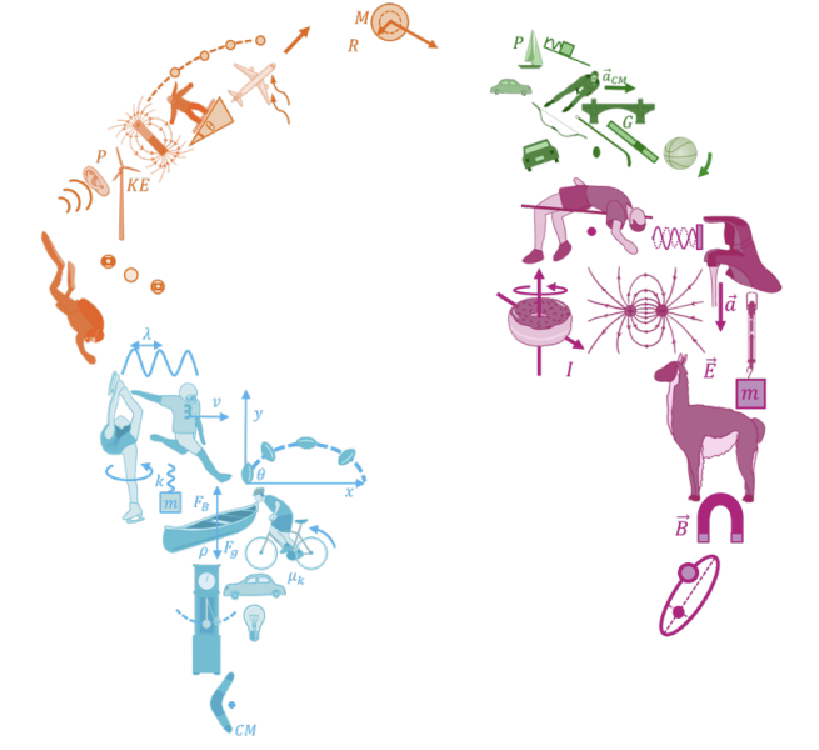
\includegraphics[width=4cm]{figures/BMDW/logo}
\end{textblock*}

\end{frame}



\twocolframe{Chapters Directory}{\thispagestyle{empty}\vspace{-0.25cm}
  \begin{enumerate}
   \item \hyperref[chap:modelandexperiment]{Model and Experiment}
   \item \hyperref[chap:math]{Mathmtical Tools and Their Use in Physics}
   \item \hyperref[chap:kinematics]{Kinematics}
   \item \hyperref[chap:newtonslaws]{Newton's Laws}
   \item \hyperref[chap:applyingnewtonslaws]{Applying Newton's Laws}
   \item \hyperref[chap:workenergy]{Work \& Energy}
   \item \hyperref[chap:potentialecon]{Potential \& Energy Conservation}
   \item \hyperref[chap:gravity]{Gravity}
   \item \hyperref[chap:momentumandcm]{Momentum and Centre of Mass}
   \item \hyperref[chap:rotationaldynamics]{Rotational Dynamics}
   \item \hyperref[chap:angularmomentumrolling]{Angular Momentum and Rolling}
  \end{enumerate}
}
{\thispagestyle{empty}\vspace{-0.25cm}
  \begin{enumerate}
 \setcounter{enumi}{11}
   \item \hyperref[chap:simpleharmonicmotion]{Simple Harmonic Motion}
   \item \hyperref[chap:waves]{Waves}
   \item \hyperref[chap:fluidmechanics]{Fluid Mechanics}
   \item \hyperref[chap:chargesandfields]{Charges and Fields}
   \item \hyperref[chap:gauss]{Gauss}
   \item \hyperref[chap:electricpotential]{Electric Potential}
   \item \hyperref[chap:current]{Current}
   \item \hyperref[chap:circuits]{Circuits}
   \item \hyperref[chap:magneticforce]{Magnetic Force}
   \item \hyperref[chap:bsource]{Sources of Magnetic Fields}
   \item \hyperref[chap:induction]{Induction}
   \item \hyperref[chap:relativity]{Relativity}
  \end{enumerate}
}




















\title{Model and Experiment}
\subject{Theories, Uncertainty, and Dimensions}
\subtitle{Building Models to Describe our World}







\begin{frame}
\label{chap:modelandexperiment}
%\chaptertitle{Model and Experiment}
\titlepage
\thispagestyle{empty}

\begin{textblock*}{5cm}(11cm,4cm)
    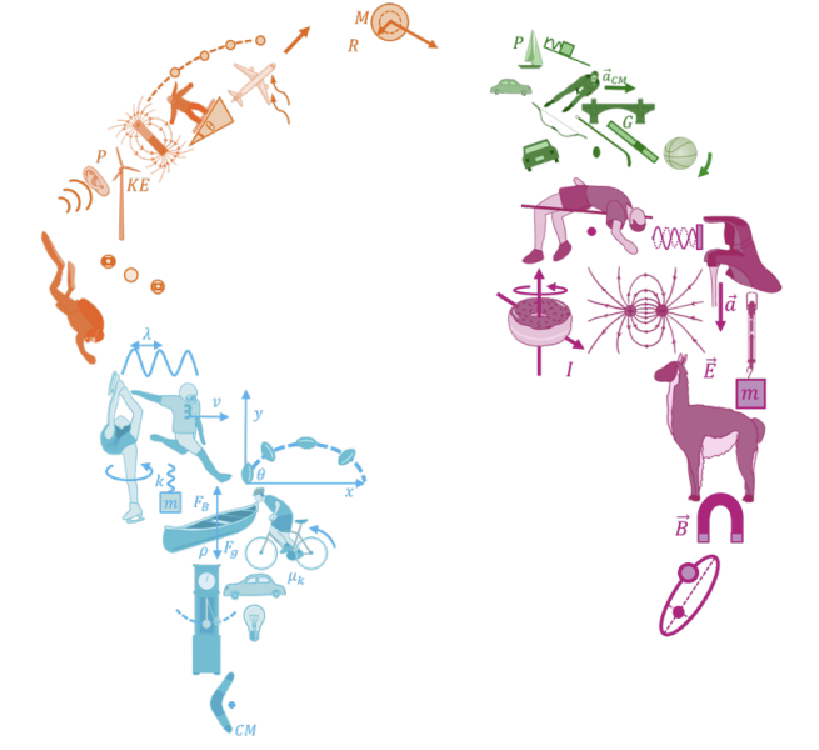
\includegraphics[width=4cm]{figures/BMDW/logo}
\end{textblock*}

\end{frame}

%%%%%%%%%%%%%TOC

\twocolframe{Outline}
{\tableofcontents[sections=1, subsectionstyle=show/show]\thispagestyle{empty}}
{\tableofcontents[sections=2-3, subsectionstyle=show/show]}

%%%%%%%%%%%%%%%%%%%%%%%%%











%%%%%%%%%%%%%%%%%%%%%%%%%%%%%%%%
\section{Building Models}
\label{sec:buildingmodels}
\title{Building Models}
\institute{Model and Experiment}
\author{\insertsubsection}


%%%%%%%%%%%%%%%%%%%%%%%%%
\begin{frame}
\titlepage
\thispagestyle{empty}
\end{frame}

%%%%%%%%%%%%%%%%%%%%%%%%%%%%






\subsection{Model vs experiment}
\label{subsec:modelvsexperiment}
\twocolframest{Model and experiment}
{
\begin{itemize}
\item We wish to test a theory, so we plan an experiment. That’s the fundamental aspect of science!
\item We use the theory to build a model and predict the result that we expect from our experiment
\item We compare the experimental result to the model prediction. Neither can ever be known with infinite precision:
\begin{itemize}
\item Model prediction depends on the assumptions that were made and uncertainties in the parameters of the model
\item Measurement depends on experimental uncertainties
\end{itemize}

\item[$\rightarrow$] Science can never make definitive statements, only statements based on probabilities (the probability that global warming is not due to human activity is very small, the probability that smoking does not cause lung cancer is very small…).
\end{itemize}
}
{  
\capfig{1}{figures/ModelAndExperiment/doubt}{}
}


%%%%%%%%%%%%%%%%%%%%%%%%%%%%%%%%
\subsection{Does my prediction make sense?}
\label{subsec:doesmypredictionmakesense}
\begin{bulletframe}{Does my model prediction make sense?}
\item Did I correctly apply the rules for using a given theory? (e.g. identify all of the forces on an object, when applying Newton’s theory)
\item Does my predicted value have the correct order of magnitude? (e.g. did I predict that a ball will fall faster than the speed of light?)
\item Does my predicted value have the correct dimension? (e.g. did I predict that it would take a time of 3m to fall a distance of 1m?)
\item Does my predicted value change as I expect that it would? (e.g. if I drop a ball from higher, does my predicted fall time increase?)
\item[$\rightarrow$] \textbf{In assignments, we will require you to include a few sentences to evaluate whether your predictions make sense.}
\end{bulletframe}


%%%%%%%%%%%%%%%%%%%%%%%%%%%%%%%%
\subsection{Base dimenions and units}
\label{subsec:basedimensionsandunits}
\twocolframesf{Base dimensions and units}
{
\begin{itemize}
\item Anything that you can measure/quantify has a dimension.
\item Multiple units can be used for the same dimension (e.g mm, ft, soccer fields are all units for the dimension of length, L).
\item We can define a set of Base Dimension, and any other dimension can always be expressed in terms of those base dimensions. (e.g the dimension of speed is L/T)
\item Base SI units are the SI units that correspond to the base dimensions. (e.g. the SI unit for speed is m/s)
\end{itemize}
}
{
\scriptsize
\begin{center}
\begin{tabular}{ll }
\textbf{Dimension}&\textbf{SI unit}\\
\hline
\hline
Length [L]& meter [m]\\ \hline
Time [T]& seconds[s] \\ \hline
Mass [M]& kilogram [kg]\\ \hline
Temperature [$\Theta$]& kelvin [K] \\ \hline
Electric current [I]& amp\`ere [A]\\ \hline
Amount of substance [N]& mole [mol] \\ \hline
Luminous intensity [J]& candela [cd] \\ \hline
Dimensionless [1]& unitless [] \\ \hline
\end{tabular}
\captionof*{table}{\label{tab:modelandexperiment:SIunits}\textit{Base dimensions and their SI units with abbreviations.}}
\end{center}
You don’t need to memorize these, you will know them with practice (in general, don’t memorize things in physics, just ask if we forgot something on the formula sheet!)
}


%%%%%%%%%%%%%%%%%%%%%%%%%%%%%%%%


%%%%%%%%%%%%%%%%%%%%%%%%%%%%%%%%
\begin{frame}{Algebra with dimensions/units}
\begin{itemize}
\item If you obtain a formula for your model prediction, that prediction will have dimensions, based on the inputs to your model
\item For example, distance, $x$, in terms of an acceleration, $g$, initial speed, $v_0$, and time, $t$:
\begin{eqnarray}
x=v_0t+\frac{1}{2}gt^2
\end{eqnarray}
\item Evaluating the dimension of $x$:
\begin{eqnarray}
[x] = [v_0][t]+\left[\frac{1}{2}\right][g][t^2]=\frac{L}{T}T+1\frac{L}{T^2}T^2=L+L
\end{eqnarray}
\item You can use the SI units instead of the dimensions, to carry out the same exercise
\item \textbf{Always check that your prediction is dimensionally correct!} It won’t guarantee that your formula is correct, but it will identify if it is definitely wrong!
\end{itemize}

\end{frame}




%%%%%%%%%%%%%%%%%%%%%%%%%%%%%%%%









%%%%%%%%%%%%%%%%%%%%%%%%%%%%%%%%
\section{Uncertainty and Error}
\label{sec:uncertaintyanderror}
\title{Uncertainty and Error}


%%%%%%%%%%%%%%%%%%%%%%%%%
\begin{frame}
\titlepage
\thispagestyle{empty}
\end{frame}

%%%%%%%%%%%%%%%%%%%%%%%%%%%%








%%%%%%%%%%%%%%%%%%%%%%%%%%
\subsection{Uncertainties}
\label{subsec:measurementuncertainty}
\begin{bulletframe}{Measurement uncertainty}
\item You can never measure anything to infinite precision.
\item You can only ever say that a value is likely within some range.
\item We communicate this as:
\begin{eqnarray}
x = (10.0\pm 0.1)\text{m}\;\;\; \rightarrow\;\;\;\text{``central value'' $\pm$ ``uncertainty''}
\end{eqnarray}
\item We mean that we are \emph{pretty confident} that $x$ is between \SI{9.9}{m} and \SI{10.1}{m}.
\item It is up to us, scientists, to \textbf{be precise} in explaining what we mean by \emph{pretty confident} $\rightarrow$ usually, we are 68\% confident. Ultimately, we need to be precise in describing how we determined the central value and uncertainty.
\end{bulletframe}


%%%%%%%%%%%%%%%%%%%%%%%%%%%%%%%%
\begin{bulletframe}{Relative uncertainty}
\item We want to know how precise our measurement is.
\item In other words, is the uncertainty large? Are we confident that the true value is close to the central value?
\item We quantify how large the uncertainty is relative to the central value $\rightarrow$ relative uncertainty:
\begin{align*}
x &=\bar x \pm \sigma_x\\
\text{Relative uncertainty} &=\frac {\sigma_x}{\bar x}=\frac{\text{uncertainty}}{\text{central value}}
\end{align*}
\item Express the relative uncertainty in percent
\item Usually, we consider 1\% relative uncertainty as precise
\item You measured that the Moon is $1\pm 1$ light years from the Earth; ok, good for you, but your very imprecise measurement is not very useful to test any model!
\end{bulletframe}

%%%%%%%%%%%%%%%%%%%%%%%%%%%%%%%%
\begin{bulletframe}{Determining an uncertainty}
\item This is by far the trickiest part of experimental physics, and usually the main focus of any experiment.
\item There is no “set in stone” rule for determining uncertainties, but there are some guidelines and accepted methods.
\item \textbf{The most important part is that you precisely describe (and justify) how you determined an uncertainty, and that you make every effort to minimize it.}
\item Ideally, if you can repeat a measurement multiple times; then this is the best way to determine an uncertainty:
\begin{itemize}
\item Mean and standard deviation (you’ll get practice in the labs next week)
\item Mean is the average, standard deviation is the average distance of measurements to the mean (whether or not the measurements are very scattered about the mean)
\end{itemize}
\item If appropriate, you can use half the smallest division of your measuring device as the uncertainty (it should rarely be smaller than this).
\end{bulletframe}

%%%%%%%%%%%%%%%%%%%%%%%%%%%%%%%%
\subsection{Precision vs accuracy  vs errors}
\label{subsec:precisionvsaccuracyvserrors}
\twocolframest{Precision and accuracy, random and systematic errors}
{
\begin{itemize}
\item You might find that multiple measurements have a small spread (and result in a small uncertainty) $\rightarrow$ Your measurements are \emph{precise}.
\item You later discover that your measurements are “way off” from the true value $\rightarrow$ Your measurements are not \emph{accurate}.
\item \textbf{Random error:} the spread in values that you get when repeating a measurement.
\item \textbf{Systematic error:} the offset of your measurement from the “true” value. In “real” science, this is very difficult to detect, since we never know the true value.
\item In first year physics, if you measure $g=5\pm 1$\si{m/s^2}, there is likely a systematic error
\end{itemize}
}
{
\capfig{1}{figures/ModelAndExperiment/precision}{Admin, W. (2024, July 23). Precision and accuracy. Portable Spectral Services. https://www.portaspecs.com/precision-and-accuracy}
}

%%%%%%%%%%%%%%%%%%%%%%%%%%%%%%%%

%%%%%%%%%%%%%%%%%%%%%%%%%%%%%%%%
\twocolframesf{Human error}
{
\begin{itemize}
\item \textbf{That’s not a thing. Don’t use that term!}
\item Do you mean that you made a mistake? Then fix it!
\item Do you mean that, due to reaction time, you have a systematic uncertainty in your time measurement? Then include that error!
\item Do you mean that, due to parallax, you have a systematic uncertainty in your length measurement? Then include that error!
\end{itemize}
}
{
}

%%%%%%%%%%%%%%%%%%%%%%%%%%%%%%%%


%%%%%%%%%%%%%%%%%%%%%%%%%%%%%%%%


%%%%%%%%%%%%%%%%%%%%%%%%%%%%%%%%
\subsection{Propogating uncertainties}
\label{subsec:propogatinguncertainties}
\twocolframesf{Propagating uncertainties}
{
\begin{itemize}
\item You measured, say, distance, $x$, and time, $t$, and want to know speed, $v$:
\begin{align*}
x&=\bar x \pm \sigma_x \\
t&=\bar t \pm \sigma_t \\
v&=v(x,t)=\frac{x}{t}=\bar v \pm \sigma_v 
\end{align*}
\item You want to propagate the uncertainties in $x$ and $t$ to determine the uncertainty in $v$
\item Derivative method + adding in quadrature:
\begin{align*}
\bar F &= F(\bar x, \bar y)\\
\sigma_F &= \sqrt{\left(\frac{\partial F}{\partial x} \sigma_x\right)^2+\left(\frac{\partial F}{\partial y} \sigma_y\right)^2}
\end{align*}
\end{itemize}
}
{
\begin{exampleblock}{When $F(x,y)\rightarrow v(x,t)$}
\begin{itemize}
\item<1-> Central value:
\begin{align*}
\bar v = \frac{\bar x}{\bar t}
\end{align*}
\item<2-> Uncertainty:
\begin{align*}
\only<2->{\sigma_v &= \sqrt{\left(\frac{\partial v}{\partial x} \sigma_x\right)^2+\left(\frac{\partial v}{\partial t} \sigma_t\right)^2}}\\
\only<3->{\frac{\partial v}{\partial x} &= \frac{\partial}{\partial x}\frac{x}{t}=\frac{1}{t}}\\
\only<4->{\frac{\partial v}{\partial t} &= \frac{\partial}{\partial t}\frac{x}{t}=\frac{-x}{t^2}}\\
\only<5->{\therefore \sigma_v &= \sqrt{\frac{1}{\bar t^2}\sigma_x^2+\frac{\bar x^2}{\bar t^4}\sigma_t^2}}
\end{align*}
\item<5> phew!
\end{itemize}
\end{exampleblock}
}

%%%%%%%%%%%%%%%%%%%%%%%%%%%%%%%%
\begin{frame}{Simple prescriptions}
\begin{itemize}
\item The derivative rule leads to simple prescriptions in most cases.
\item In practice, we’ll show you how to use a computer and QExpy to propagate uncertainties (see Appendix D).
\end{itemize}
\capfig{1}{figures/ModelAndExperiment/table}{}
\end{frame}

%%%%%%%%%%%%%%%%%%%%%%%%%%%%%%%%


%%%%%%%%%%%%%%%%%%%%%%%%%%%%%%%%






%%%%%%%%%%%%%%%%%%%%%%%%%%%%%%%%
\section{Dimensional Analysis}
\label{sec:dimensionalanalysis}
\title{Dimensional Analysis}
\institute{Model and Experiment}
\author{\insertsubsection}


%%%%%%%%%%%%%%%%%%%%%%%%%
\begin{frame}
\titlepage
\thispagestyle{empty}
\end{frame}

%%%%%%%%%%%%%%%%%%%%%%%%%%%%






%%%%%%%%%%%%%%%%%%%%%%%%%%%%%%%

\twocolframesf{Dimensional analysis}
{
\begin{itemize}
\item Sometimes, you know that a certain quantity, $z$, must depend on other quantities, $x$ and $y$, but you have no idea how to model it:
\begin{eqnarray*}
z=f(x,y)=x^ay^b
\end{eqnarray*}
\item As a minimum, you know that you must combine $x$ and $y$ in a way that the combination has the dimensions of $z$, but you want to know the powers, $a$ and $b$. 
\item Suppose that:
\begin{eqnarray*}
[z]=\frac{L}{T^2},\quad [x]=M\quad [y]=\frac{ML}{T^2}
\end{eqnarray*}
\end{itemize}
}
{
\begin{exampleblock}{Determining $a$ and $b$}
\begin{itemize}
\item<1-> $[z] = [x]^a[y]^b$
\item<2-> $\frac{L}{T^2}=(M)^a\left(\frac{ML}{T^2} \right)^b=(M)^{a+b}\frac{L^{b}}{T^{2b}}$
\item<3->[$\rightarrow$] Equate powers of $L$, $T$ and $M$ on both sides:
\item<4-> On the left, $M$ is to the power of 0 (there are no $M$s) and $M$ is to the power $a+b$ on the right. These must be the same:\\
$0=a+b$
\item<5-> Same with $L$ (1 on the left, $b$ on the right):\\
$1=b$
\item<6->[$\rightarrow$] $b=1$ and $a=-1$. $f(x,y)=x^ay^b$ must thus be of the form:
\begin{eqnarray*}
z = x^{-1}y^{1}=\frac{y}{x}
\end{eqnarray*}
\end{itemize}

\end{exampleblock}
}

%%%%%%%%%%%%%%%%%%%%%%%%%%%%%%%%



%%%%%%%%%%%%%%%%%%%%%%%%%%%%%%%%



%%%%%%%%%%%%%%%%%%%%%%%%%%%%%%%%
























%Frames:
% \twocolframesf 60/40 (fs, st, ts) 
% \titleframe
% bulletframe

%%%%%%%%%%%%%%%%%%%%%%%%%
%%%%%% START OF PRESENTATION %%%%%%
%%%%%%%%%%%%%%%%%%%%%%%%%

\title{Mathmatical Tools and Their Use in Physics}
\subject{Vectors and Calculus}
\subtitle{Building Models to Describe our World}


\begin{frame}
\label{chap:math}
%\chaptertitle{Mathmatical Tools and Their Use in Physics}
\titlepage
\thispagestyle{empty}

\begin{textblock*}{5cm}(11cm,4cm)
    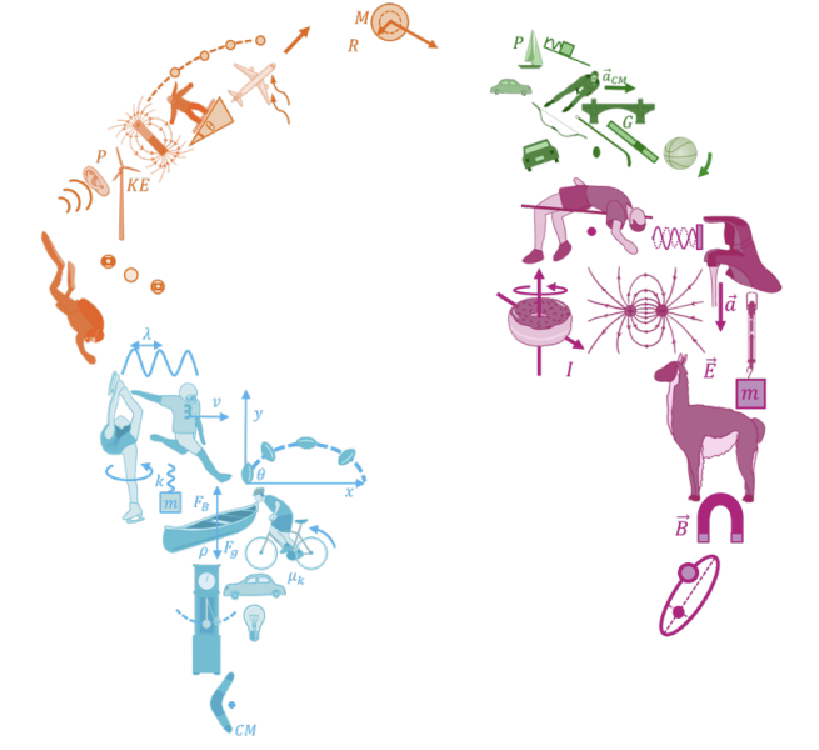
\includegraphics[width=4cm]{figures/BMDW/logo}
\end{textblock*}

\end{frame}

%%%%%%%%%%%%%%%%%%%%%%%%%%%%%
\twocolframe{Outline}
{\tableofcontents[sections=4-5, subsectionstyle=show/show]\thispagestyle{empty}}
{\tableofcontents[sections=6, subsectionstyle=show/show]}


%%%%%%%%%%%%

%%%%%%%%%%%%%%%%%%%%%%%%%%%
\section{Vectors}
\label{sec:vectors}
\title{Vectors}


%%%%%%%%%%%%%%%%%%%%%%%%%
%%%%%% Title slide %%%%%%
%%%%%%%%%%%%%%%%%%%%%%%%%
\begin{frame}
\titlepage
\thispagestyle{empty}
\end{frame}

%%%%%%%%%%%%%%%%%%%%%%%%%%%%%%%%
%%Advertisements and such %%%%%%
%%%%%%%%%%%%%%%%%%%%%%%%%%%%%%%%

%%%%%%%%%%%%%%
%\colloquium{title}
%{\small
%abstract
% }
%{scale}
%{figures/speaker}
%{\small \textbf{author},institute }
%

%%%%%%%%%%%%%%%%%%%%%%%%%%%%%%%%%%%%%%%%%%%%%%%%%%%%%%%%%%%%%%%%%%%%%%%%%%%%%%%%%%%%%%%
%%%%%%%%%%%%%%%%%%%%%%%%%%%%%%%%
%% Actual lecture slides  %%%%%%
%%%%%%%%%%%%%%%%%%%%%%%%%%%%%%%%



%%%%%%%%%%%%%%%%%%%%%%%%%%%%%%%%
\subsection{Coordinate systems}
\label{subsec:coordinatesystems}
\twocolframesf{Coordinate systems}
{
\begin{itemize}
\item Because we want to describe things in space, and we live in 3 dimensions!
\item In practice, we can often simplify and use 1D or 2D coordinate systems.
\item The most common type of coordinate system is a right-handed Cartesian coordinate system, where you must specify:
\begin{itemize}
\item 3 mutually perpendicular axes/directions (specify 2, the third is given by the right hand rule).
\item 1 fixed origin.
\end{itemize}
\item Using a coordinate system, can specify the position of a point using its \textbf{coordinates}.
\item Can you think of an example where you've used spherical coordinates?
\end{itemize}
}
{
\centering
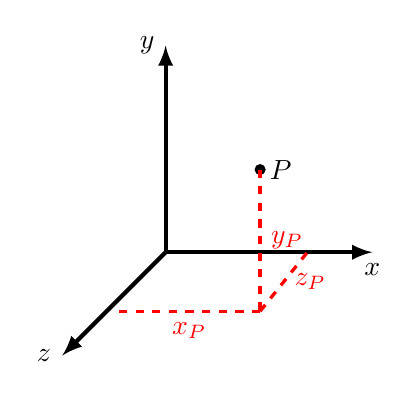
\begin{tikzpicture}[scale=1]
\tikzmath{
\R=1.5;
\f=0.5;
\fx=\f+1;
}
\scalebox{1.0}{

\coordinate (P) at (0.8*\R,0.7*\R);
\coordinate (PP) at (0.8*\R,-0.5*\R);
\coordinate (PX) at (0.8*\R*\fx,0);
\coordinate (PZ) at (-\f*0.8*\R,-0.5*\R);
 %axes:
 \draw[-latex, line width=1.5pt] (0,0) -- (1.75*\R,0) node[below]{$x$}; 
 \draw[-latex, line width=1.5pt] (0,0) -- (0,1.75*\R) node[left]{$y$}; 
 \draw[-latex, line width=1.5pt] (0,0) -- (-\f*1.75*\R,-\f*1.75*\R) node[left]{$z$};  
 
 %point
 \fill (P) circle(2pt);
 \node[right] at (P) {$P$};
 
 %dotted lines
 \draw[dashed,color=red,line width=1.2pt] (P) -- (PP) node[midway,right]{$y_P$};
 \draw[dashed,color=red,line width=1.2pt] (PP) -- (PX) node[midway,right]{$z_P$};
 \draw[dashed,color=red,line width=1.2pt] (PP) -- (PZ) node[midway,below]{$x_P$};
}
\end{tikzpicture}
\captionof*{figure}{\textit{A \textbf{right-handed} Cartesian coordinate system, where $\hat x \times \hat y = \hat z$. ($\hat z$ is out of the page). The point $P$ has coordinates $(x_P,y_P,z_P)$.}}
}

%%%%%%%%%%%%%%%%%%%%%%%%%%%%%%%%
\subsection{Vector basics}
\label{subsec:vectorbasics}
\twocolframest{Vectors}
{
\begin{itemize}
\item Vectors are arrows with a magnitude and a direction.
\item They are useful for describing quantities with a magnitude and a direction:
\begin{itemize}
\item A displacement.
\item A velocity.
\item A force.
\item An angular velocity.
\end{itemize}
\item We can describe a vector by specifying its \textbf{components}, or its magnitude and direction(s) (in 3D, need magnitude and two angles).
\item Notation:
\end{itemize}
\begin{align*}
\vec v = v_x\hat x+v_y\hat y+v_z\hat z=(v_x,v_y,v_z)=\begin{pmatrix}
v_x\\v_y\\v_z
\end{pmatrix}
\end{align*}
}
{
\centering
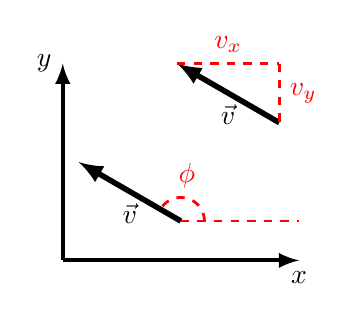
\begin{tikzpicture}[scale=1]
\tikzmath{
\L=2.5;
\v=1.5;
}
\scalebox{1.0}{

 \coordinate (P1) at (1.1*\L,0.7*\L);
 \coordinate (P2) at ($(P1)+(-0.5*\L,-0.5*\L)$);
 
 %axes:
 \draw[-latex, line width=1.5pt] (0,0) -- (1.2*\L,0) node[below]{$x$}; 
 \draw[-latex, line width=1.5pt] (0,0) -- (0,\L) node[left]{$y$}; 
 
 \draw[-latex,line width=2pt] (P1) -- ($(P1)+(150:\v)$) node[midway,below]{$\vec v$};
 \draw[dashed,line width=1pt,color=red] ($(P1)+(150:\v)$) -- ($(P1)+(150:\v)+cos(30)*(\v,0)$) node[midway, above] {$v_x$};
 \draw[dashed,line width=1pt,color=red] ($(P1)+(150:\v)+cos(30)*(\v,0)$) --(P1) node[midway, right] {$v_y$};
 
 \draw[-latex,line width=2pt] (P2) -- ($(P2)+(150:\v)$) node[midway,below]{$\vec v$};
 \draw[dashed,line width=1pt,color=red] (P2) -- ($(P2)+(0:\v)$);
 \draw[dashed,line width=1pt,color=red] ($(P2)+(0.2*\v,0)$) arc (0:150:0.2*\v) node[midway, above] {$\phi$};;
}
\end{tikzpicture}
\captionof*{figure}{\textit{A vector in 2D can be specified by two Cartesian components ($v_x,v_y$) or its length, $v$, and an angle with respect to the $x$ direction, $\phi$.}}
}


%%%%%%%%%%%%%%%%%%%%%%%%%%%%%%%%




%%%%%%%%%%%%%%%%%%%%%%%%%%%%%%%%
\begin{bulletframe}{Algebra with vectors}
 \item You can multiply/divide a vector by \textbf{a scalar}.
 \item You cannot add a scalar to a vector (as with anything, you cannot add oranges and apples).
 \item You can add/subtract two vectors (of the same dimensions, e.g. 2D or 3D).
 \item Two ways to multiply vectors:
 \begin{itemize}
   \item Scalar/dot product $\rightarrow$ the result is a scalar.
 \item Vector/cross product $\rightarrow$ the results is a vector (and this requires 3D and a flexible wrist).
 \end{itemize}
\end{bulletframe}

%%%%%%%%%%%%%%%%%%%%%%%%%%%%%%%%
%%%%%%%%%%%%%%%%%%%%%%%

%%%%%%%%%%%%%%%%%%%%%%%%%%%%%%%%
\twocolframesf{Vector addition and vector equations}
{
\scriptsize
\begin{itemize}
\item To add vectors $\vec a$ and $\vec b$:
\begin{itemize}
\scriptsize
\item Graphically, place them head to tail.
\item Algebraically, add the components together.
\end{itemize}
\item The ``unit vector'' notation for a vector is just vector addition:
\begin{align*}
\vec a = a_x \hat x + a_y \hat y
\end{align*}
\item<2-> \textbf{An equation with vectors is a short-hand for equations between components:}
\begin{align*}
\vec c = \vec a + 2\vec b
\end{align*}
\emph{is the same as the two independent equations:}
\begin{align*}
c_x &= a_x + 2b_x\\
c_y &= a_y+2b_y
\end{align*}
\end{itemize}
}
{
\centering
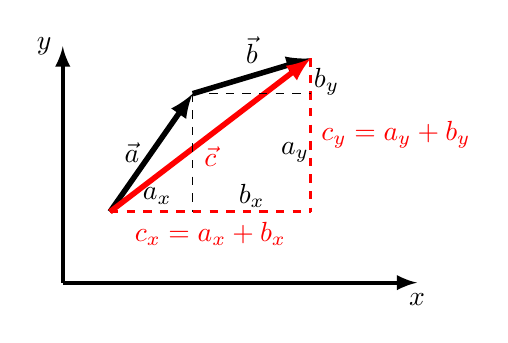
\begin{tikzpicture}[scale=1]
\tikzmath{
\L=3.;
\u=\L/2;
}
\scalebox{1.0}{

 \coordinate (P) at (0.2*\L,0.3*\L);
 \coordinate (PA) at ($(P)+(0.7*\u,\u)$);
 \coordinate (PC) at ($(PA)+(1.0*\u,0.3*\u)$);
 \coordinate (PAX) at ($(P)+(0.7*\u,0)$);
 \coordinate (PBY) at ($(PC)+(0,-0.3*\u)$);
 %axes:
 \draw[-latex, line width=1.5pt] (0,0) -- (1.5*\L,0) node[below]{$x$}; 
 \draw[-latex, line width=1.5pt] (0,0) -- (0,\L) node[left]{$y$}; 
 
 \draw[-latex,line width=2pt] (P) -- (PA) node[midway,left]{$\vec a$};
 \draw[-latex,line width=2pt] (PA) -- (PC) node[midway,above]{$\vec b$};
 \draw[-latex,line width=2pt, color=red] (P) -- (PC) node[midway,below]{$\vec c$};
 
 \only<2>{
 \draw[dashed, line width=1.0, color=red] (P) -- ($(P)+(1.7*\u,0)$) node[midway,below]{$c_x=a_x+b_x$};
 \draw[dashed, line width=1.0, color=red] (PC) -- ($(PC)+(0,-1.3*\u)$)node[midway,right]{$c_y=a_y+b_y$};
 
 \draw[dashed] (PA) -- (PAX);
 \draw[dashed] (PA) -- (PBY);
 
 \node at ($(PAX)+(-0.3*\u,0.2)$) {$a_x$};
 \node at ($(PAX)+(0.5*\u,0.2)$) {$b_x$};
 \node at ($(PBY)+(-0.2,-0.5*\u)$) {$a_y$};
 \node at ($(PBY)+(0.2,0.1*\u)$) {$b_y$};
 }
}
\end{tikzpicture}
\captionof*{figure}{\textit{A graphical illustration of $\vec c = \vec a + \vec b$.}}
}

%%%%%%%%%%%%%%%%%%%%%%%%%%%%%%%%
\subsection{Scalar Product}
\label{subsec:scalarproduct}
\twocolframest{Scalar product}
{
%\scriptsize
\begin{itemize}
\item Scalar product is a sum of the components of the two vectors multiplied together (commutative):
\begin{align*}
\vec a \cdot \vec b = a_xb_x+a_yb_y+a_zc_z=\vec b \cdot \vec a
\end{align*}
\item It is also proportional to the cosine of the angle between the vectors (if these are placed tail to tail):
\begin{align*}
\vec a \cdot \vec b = ab\cos\theta
\end{align*}
\item It is thus zero if two vectors are perpendicular to each other, $\cos(90)=0$
\item By knowing the components of two vectors, you can determine their scalar product, and then the angle between the two vectors
\end{itemize}
}
{
\centering
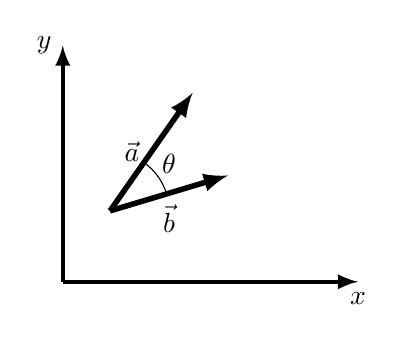
\begin{tikzpicture}[scale=1]
\tikzmath{
\L=3.;
\u=\L/2;
}
\scalebox{1.0}{

 \coordinate (P) at (0.2*\L,0.3*\L);
 \coordinate (PA) at ($(P)+(0.7*\u,\u)$);
 \coordinate (PB) at ($(P)+(1.0*\u,0.3*\u)$);

 %axes:
 \draw[-latex, line width=1.5pt] (0,0) -- (1.25*\L,0) node[below]{$x$}; 
 \draw[-latex, line width=1.5pt] (0,0) -- (0,\L) node[left]{$y$}; 
 
 \draw[-latex,line width=2pt] (P) -- (PA) node[midway,left]{$\vec a$};
 \draw[-latex,line width=2pt] (P) -- (PB) node[midway,below]{$\vec b$};
 
 \node at ($(P)+(0.5*\u,0.4*\u)$){$\theta$};
 \path[clip] (P) -- (PA) -- (PB) -- cycle;
 \draw ($(P)+(0.5*\u,0)$) arc (0:90:0.5*\u);

 

}
\end{tikzpicture}
\captionof*{figure}{\textit{The scalar product between vectors depends on the angle between them when they are placed tail to tail.}}
}

%%%%%%%%%%%%%%%%%%%%%%%%%%%%%%%%

%%%%%%%%%%%%%%%%%%%%%%%%%%%%%%%%
\subsection{Cross-Product}
\label{subsec:crossproduct}
\twocolframesf{Cross-product}
{
\scriptsize
\begin{itemize}
\item The cross product gives a \textbf{vector} that is perpendicular to the original two vectors (not commutative):
\begin{align*}
\vec a \times \vec b = \vec c = -\vec b \times \vec a
\end{align*}
\item The magnitude is related to the sine of the angle between the two original vectors:
\begin{align*}
||\vec a \times \vec b ||= ab\sin\theta
\end{align*}
\item The cross-product is zero if the two vectors are parallel or anti-parallel ($\sin 0 =0$)
\item The direction of the cross product can be found using the right hand rule
\item Cross products are always in 3D
\end{itemize}
}
{
\scriptsize
You can find the components of the cross product algebraically:
\begin{align*}
\vec a \times \vec b =\begin{pmatrix}
           a_yb_z - a_z b_y\\
           a_zb_x - a_x b_z\\
           a_xb_y - a_y b_x\\
         \end{pmatrix}
\end{align*}
or using the right-hand rule for cross-products for the direction:
\capfig{1}{figures/Math/righthandrule}{}
}
\label{fig:math:righthandrule}
%%%%%%%%%%%%%%%%%%%%%%%%%%%%%%%%


%%%%%%%%%%%%%%%%%%%%%%%%%%%%%%%%
\twocolframesf{Scalar and cross product in action}
{

Scalar product:
\begin{itemize}
\item Maximal when two vectors are parallel.
\item Zero when two vectors are perpendicular.
\item Application: ``Work''.
\end{itemize}
\vspace{1cm}
Cross product:
\begin{itemize}
\item Maximal when two vectors are perpendicular.
\item Zero when two vectors are parallel.
\item Application: ``Torque''.
\end{itemize}
}
{
\centering
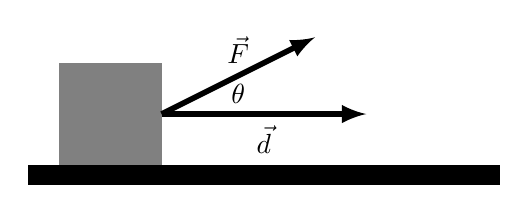
\begin{tikzpicture}[scale=1]
\tikzmath{
\L=3.;
\w=0.25;
\a=1.3;
}
\scalebox{1.0}{

\fill (-\L,-\w) rectangle (\L,0);
\fill[black!50] (-2*\a,0) rectangle (-\a,\a);

\draw[-latex,line width=2pt] (-\a,\a/2) -- +(1.5*\a,0.75*\a) node[midway,above] {$\vec F$};
\draw[-latex,line width=2pt] (-\a,\a/2) -- +(2*\a,0) node[midway,below] {$\vec d$};
\node at ($(-\a,\a/2)+(0.75*\a,0.2*\a)$) {$\theta$};
}
\end{tikzpicture}
\captionof*{figure}{\textit{The scalar product between force and displacement, $W=\vec F \cdot \vec d=Fd\cos\theta$ (Work) tells us about the change in speed.}}

\centering
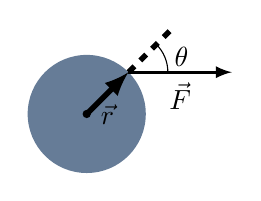
\begin{tikzpicture}[scale=1]
\tikzmath{
\R=0.75;
}
\scalebox{1.0}{

\fill[color=myblue!60] circle (\R);
\fill[] circle (1.5pt);

\draw[-latex, line width = 2pt] (0,0) -- (45:\R) node[midway, below]{$\vec r$};
\draw[dashed, line width = 2pt] (45:\R) -- + (45:\R);
\draw ($(45:\R)+(0.5,0)$) arc (0:45:0.5) node[midway, right]{$\theta$};
\draw[-latex, line width = 1pt] (45:\R) -- + (1.75*\R,0) node[midway, below]{$\vec F$};

}
\end{tikzpicture}
\captionof*{figure}{\textit{The magnitude of cross product between a force, $\vec F$, and the position vector, $\vec r$, where the force is applied tells us the angular acceleration of an object: $||\vec r \times \vec F||=rF\sin\theta$.}}

}


%%%%%%%%%%%%%%%%%%%%%%%%%%%%%%%%
\subsection{Vectors to indicate rotation}
\label{subsec:rotationvectors}
\twocolframesf{Vectors to indicate rotation}
{
\begin{itemize}
\item Suppose that you need to describe a rotating wheel to someone over the phone.
\item You need to specify:
\begin{itemize}
\item The axis of rotation (a line)
\item How fast (e.g. rotations per minute)
\item Which direction (clockwise/counter clockwise) about that axis
\end{itemize}
\item This can be specified by an “axial vector”, and the “right hand rule for axial vectors”:
\begin{itemize}
\item The vector is co-linear with the axis of rotation
\item The magnitude is proportional to rotational speed
\item The direction of the vector is given by the right hand rule for axial vectors.
\end{itemize}
\end{itemize}
}
{
\capfig{0.75}{figures/Math/righthandruleaxial}{}
\label{fig:math:righthandruleaxial}
\capfig{0.9}{figures/Math/carwheelrotation}{}
\label{fig:math:carwheelrotation}
}
%%%%%%%%%%%%%%%%%%%%%%%%%%
\section{Derivatives}
\label{sec:derivatives}
\title{Derivatives}
\institute{Mathmatical Tools and Their Use In Physics}
\author{\insertsubsection}
%%%%%%%%%%%%%%%%%%%%%%%%%%%%%%%%%%%


\begin{frame}
\titlepage
\thispagestyle{empty}
\end{frame}

%%%%%%%%%%%%%%%%%%%%%%%%%%%%%%%%%%%
\subsection{Functions}
\label{subsec:functions}
\begin{bulletframe}{Functions}
 \item We will mostly concern ourselves with functions that are mappings from a set of independent variables (x, y , z, t) to (usually) a real number.
 \item Examples of functions in physics:
 \begin{itemize}
  \item Position as a function of time for an accelerating object: $x(t)=x_0+v_{x0}t+\frac{1}{2}a_xt^2$
 \item The restoring force from a spring: $F(x) = -kx$
 \item The potential energy from gravity near Earth’s surface: $V(h) = mgh$ 
 \item The electric field from a point charge at the origin: 
 \begin{align*}
 \vec E(x,y,z) =\frac{kq}{x ^2+y^2+z^2}\hat r \quad \text{(this is one is not a mapping to a real number!)}
 \end{align*} 
\item etc….
 \end{itemize}
\end{bulletframe}


%%%%%%%%%%%%%%%%%%%%%%%%%%%%%%%%
\begin{bulletframe}{Properties of a function}
 \item When you encounter a function, ask yourself:
 \begin{itemize}
  \item Is the function ever equal to zero (what are its “roots”)?
 \item Is the function continuous for all values of the independent variables?
 \item Are there maxima/minima in the function?
 \item Is the function always defined? This is especially important in physics. We need functions to represent physical quantities, so we need to understand when they are undefined
 \end{itemize}
 \item The best thing to do is to sketch out the function to get a sense of it $\rightarrow$ There are many online tools (e.g. Wolfram alpha, Jupyter notebooks, etc)
\end{bulletframe}


%%%%%%%%%%%%%%%%%%%%%%%%%%%%%%%%



%%%%%%%%%%%%%%%%%%%%%%%%%%%%%%%%
\subsection{The derivative}
\label{subsec:thederrivative}
\twocolframesf{The derivative}
{
\begin{itemize}
\item The derivative of a function, $f(x)$, is the slope of the function (``rise over run'').
\item It tells us how steep the function is, namely, how fast it is increasing or decreasing, or neither $\rightarrow$ the rate of change of $f(x)$ with respect to $x$.
\item The derivative of a function is a function.
\item Different notations for the derivative of $f(x)$ with respect to $x$: \\\
$f'(x)$, $\frac{df}{dx}$, $\frac{d}{dx} f(x)$   
\item It tells us the (tangent of the) angle which the tangent to the function makes with the x-axis.
\end{itemize}
}
{
\centering
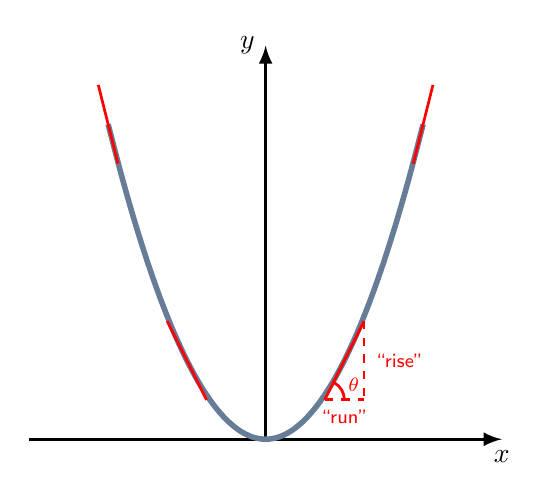
\begin{tikzpicture}[scale=1]
\tikzmath{
}
\scalebox{1.0}{
 \coordinate (P) at (1,1);
 \coordinate (P2) at (-1,1);
 \coordinate (P3) at (-2,4);
 \coordinate (P4) at (2,4);
 %axes:
 \draw[-latex, line width=1.25pt] (-3,0) -- (3,0) node[below]{$x$}; 
 \draw[-latex, line width=1.25pt] (0,0) -- (0,5) node[left]{$y$}; 
 
 %function
 \draw[scale=1, domain=-2.:2., smooth, variable=\x, line width=2,color=myblue!60] plot ({\x}, {\x*\x});
 
 
 \draw[red, line width=1] ($(P)-(0.25,0.5)$) -- ($(P)+(0.25,0.5)$);
 \draw[red, dashed, line width=1] ($(P)-(0.25,0.5)$) --  +(0.5,0) node[midway,below]{\scriptsize ``run''};
 \draw[red, dashed, line width=1] ($(P)+(0.25,0.5)$) --  +(0,-1) node[midway,right]{\scriptsize ``rise''};
 
 \draw[red, line width =1] ($(P)-(0.25,0.5)+(0.25,0)$) arc (0:60:0.25) node[midway,above=2pt,right=-1.5pt] {\scriptsize $\theta$};
 
 \draw[red, line width=1] ($(P2)-(0.25,-0.5)$) -- ($(P2)+(0.25,-0.5)$);
 \draw[red, line width=1] ($(P3)-(0.125,-0.5)$) -- ($(P3)+(0.125,-0.5)$);
 \draw[red, line width=1] ($(P4)-(0.125,0.5)$) -- ($(P4)+(0.125,0.5)$);
}
\end{tikzpicture}
\captionof*{figure}{\textit{The derivative of the function is given by the ``rise over the run''. This corresponds to the tangent of the angle that the tangent to the function makes at that point.}}
}

%%%%%%%%%%%%%%%%%%%%%%%%%%%%%%%%
\twocolframesf{The derivative is the \emph{instantaneous} rate of change of a function}
{
\begin{itemize}
\item It tells us how much $f(x)$ changes, when we change $x$, at some point $x$.
\item That is, it tells us the value of $\Delta f$ if we go from $x$ to $x+\Delta x$.
\item Suppose that we choose two points, $x_1$  and $x_2$, separated by a distance $\Delta x$:
\begin{align*}
\Delta x &= x_2-x_1,\quad f(x_1) = f_1, \quad f(x_2)=f_2\\
\Delta f &=f_2-f_1\\
\therefore f'(x) &= \frac{df}{dx}=\lim_{\Delta x\to 0}\frac{\Delta f}{\Delta x}=\lim_{\Delta x\to 0}\frac{f(x+\Delta x)-f(x)}{\Delta x}
\end{align*}
 
\end{itemize}
}
{
\centering
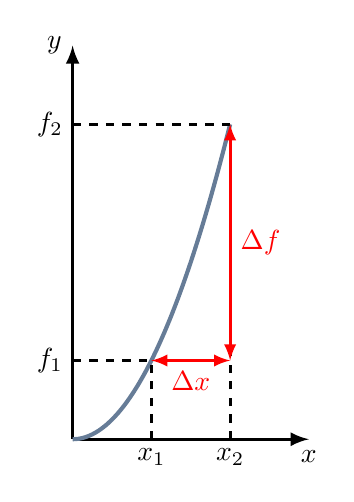
\begin{tikzpicture}[scale=1]
\tikzmath{
}
\scalebox{1.0}{
 \coordinate (P) at (1,1);

 %axes:
 \draw[-latex, line width=1.25pt] (0,0) -- (3,0) node[below]{$x$}; 
 \draw[-latex, line width=1.25pt] (0,0) -- (0,5) node[left]{$y$}; 
 
 %function
 \draw[scale=1, domain=0.:2., smooth, variable=\x, line width=1.5,color=myblue!60] plot ({\x}, {\x*\x});
 
 \node[below] at (1,0) {$x_1$};
 \node[below] at (2,0) {$x_2$};
 \node[left] at (0,1) {$f_1$};
 \node[left] at (0,4) {$f_2$};
 
 \draw[dashed,line width =1] (1,0) -- (1,1);
 \draw[dashed,line width =1] (2,0) -- (2,4);
 \draw[dashed,line width =1] (0,1) -- (1,1);
 \draw[dashed,line width =1] (0,4) -- (2,4);
 
 \draw[latex-latex,red, line width=1] (1,1) -- +(1,0) node[midway,below]{$\Delta x$};
 \draw[latex-latex,red, line width=1] (2,4) -- +(0,-3) node[midway,right]{$\Delta f$};
}
\end{tikzpicture}
\captionof*{figure}{\textit{The derivative of the function is given by $\frac{\Delta f}{\Delta x}$ in the limit where $\Delta x \to 0$.}}
}

%%%%%%%%%%%%%%%%%%%%%%%%%%%%%%%%



%%%%%%%%%%%%%%%%%%%%%%%%%%%%%%%%
\subsection{How to find a derivative}
\label{subsec:howtofindder}
\begin{frame}{How to find a derivative}
\begin{itemize}
\item You’ll learn in calculus (the textbook shows how to do derive it for the case of $f(x)=x^2$).
\item For now, you need to know where to look them up, and how to apply the rules:
\end{itemize}
\centering
\only<1>{
\begin{tabular}{l l}
\textbf{Function, $f(x)$} & \textbf{Derivative, $f'(x)$}\\
\hline\hline
$f(x)=a$ & $f'(x)=0$ \\
$f(x)=x^n$ & $f'(x)=nx^{n-1}$ \\
$f(x)=\sin(x)$ & $f'(x)=\cos(x)$ \\
$f(x)=\cos(x)$ & $f'(x)=-\sin(x)$ \\
$f(x)=\tan(x)$ & $f'(x)=\frac{1}{\cos^2(x)}$ \\
$f(x)=e^x$ & $f'(x)=e^x$ \\
$f(x)=\ln(x)$ & $f'(x)=\frac{1}{x}$ \\
\hline
\end{tabular}
\captionof*{table}{\label{tab:Calculus:commonders}Common derivatives of functions.}}
\only<2>{
\begin{tabular}{l l}
\textbf{Function, $h(x)$} & \textbf{Derivative, $h'(x)$}\\
\hline\hline
$h(x)=f(x)+g(x)$ & $h'(x)=f'(x)+g'(x)$ \\
$h(x)=f(x)-g(x)$ & $h'(x)=f'(x)-g'(x)$ \\
$h(x)=f(x)g(x)$ & $h'(x)=f'(x)g(x)+f(x)g'(x)$ (The product rule) \\
$h(x)=\frac{f(x)}{g(x)}$ & $h'(x)=\frac{f'(x)g(x)-f(x)g'(x)}{g^2(x)}$ (The quotient rule)\\
$h(x)=f(g(x))$ & $h'(x)=f'(g(x))g'(x)$ (The Chain Rule) \\
\hline
\end{tabular}
\captionof*{table}{\label{tab:Calculus:combders}Derivatives of combined functions.}
}
\end{frame}

%%%%%%%%%%%%%%%%%%%%%%%%%%%%%%%%



%%%%%%%%%%%%%%%%%%%%%%%%%%%%%%%%
\begin{bulletframe}{Inifinitesimals - Calculus notation}
\scriptsize
\item Calculus usually involves asking what happens when something is very small
\item The derivative is:
\begin{align*}
f'(x) =\lim_{\Delta x\to 0}\frac{\Delta f}{\Delta x}
\end{align*}
\item We write this as:
\begin{align*}
f'(x) =\frac{df}{dx}
\end{align*}
\item You can really think of $dx$ as a very small $\Delta x$, and $df$ as the \emph{correspondingly} small $\Delta f$.
\item You can multiply them out:
\begin{align*}
f'(x) dx=df
\end{align*}
\item You can cancel them out:
\begin{align*}
\frac{df}{dg}\frac{dg}{dx}=\frac{df}{dx}
\end{align*}
\item This works because 
\begin{align*}
dx=\lim_{\Delta x\to 0} \Delta x
\end{align*}
(your math friends are cringing…) 
\end{bulletframe}


%%%%%%%%%%%%%%%%%%%%%%%%%%%%%%%%
\subsection{Functions of multiple variables}
\label{subsec:multvarfuncs}
\twocolframe{Functions of multiple variables}
{
\only<1>{
\begin{itemize}
\item Many quantities depend on where you are in space (i.e. a function of x,y,z).
\item These become difficult to visualize...
\item We have to define the rate of change of the function in any direction...
\item In the plot, at point $P$:
\begin{itemize}
\item The function decreases as $x$ increases (if $y$ is held fixed, dashed red line).
\item The function increases as $y$ increases (if $x$ is held fixed, solid red line).
\end{itemize}
\end{itemize}
}
\only<2>{
\begin{itemize}
\item The partial derivative of $f(x, y)$ with respect to $x$ tells us the rate of change of $f$ as a function of $x$ if we hold $y$ constant (following the dashed line).
\item The partial derivative of $f(x, y)$ with respect to $y$ tells us the rate of change of $f$ as a function of $y$ if we hold $x$ constant (following the solid line).
\item There are $n$ partial derivatives if there are $n$ independent variables.
\item Each partial derivative is a new function of the $n$ variables.
\end{itemize}
}
\only<3>{
Notation:
\begin{align*}
f(x,y)&=x^2-2y^2\\
\therefore\frac{\partial f}{\partial x}&=\frac{\partial}{\partial x}x^2-2y^2=2x\\
\therefore\frac{\partial f}{\partial y}&=\frac{\partial}{\partial y}x^2-2y^2=-4y;
\end{align*}
\begin{itemize}
\item Pronounced ``die f by die x''.
\item Calculate a partial derivative exactly the same way that you would a normal derivative (treat all other independent variables as constants).
\end{itemize}
}

}
{
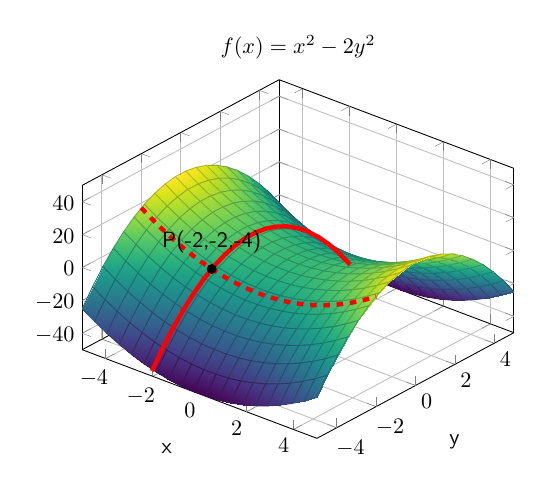
\begin{tikzpicture}[scale=0.8]

\begin{axis}[
  colormap/viridis,  
  view = {40}{40},
	xmax = 5,
	xmin = -5,
	ymax = 5, 
	ymin = -5, 
	zmax = 50, 
	zmin = -50,
	xtick = {-4,-2,0,2,4},
	ytick = {-4,-2,0,2,4},
	ztick = {-40,-20,0,20,40},
	xlabel={x},
	ylabel={y},
	title={$f(x)=x^2-2y^2$},
	grid]
	

\addplot3 [
	domain=-5:5,
	domain y = -5:5,
	samples = 20,
	samples y = 20,
	surf,
	shader =faceted interp] {x^2 -2*y^2};
	
\addplot3 [
	domain=-5:5,
	samples = 20,
	samples y = 1,
	line width =2,
	color=red,
	dashed,
	smooth] (x,-2,{x^2 -8});
	
\addplot3 [
	domain y =-5:5,
	samples = 1,
	samples y = 20,
	line width =2,
	color=red,
	smooth] (-2,y,{4 -2*y^2});	
	
\node[label={P(-2,-2,-4)}] at (-2,-2,-4) {};
\draw plot [mark=*, mark size=2] coordinates{(-2,-2,-4)}; 

\end{axis}

\end{tikzpicture}
\captionof*{figure}{\textit{A point, $P$, is on the surface given by $f(x,y)=x^2-2y^2$.}}
}


%%%%%%%%%%%%%%%%%%%%%%%%%%%%%%%%
\subsection{The gradient vector}
\label{subsec:gradientvector}
\twocolframe{The gradient vector}
{
\begin{itemize}
\item From the partial derivatives, we know how the function changes along the x and y directions.
\item The gradient tells us the direction in which the function changes the fastest, with components given by the partial derivatives.
\item It is a vector whose magnitude tells us how fast the function is changing in the direction of maximal change.
\begin{align*}
\nabla f(x,y) &= \frac{\partial f}{\partial x} \hat x + \frac{\partial f}{\partial y}\hat y\\
&=2x\hat x - 4y \hat y = (-4,8)
\end{align*}
\end{itemize}
}
{
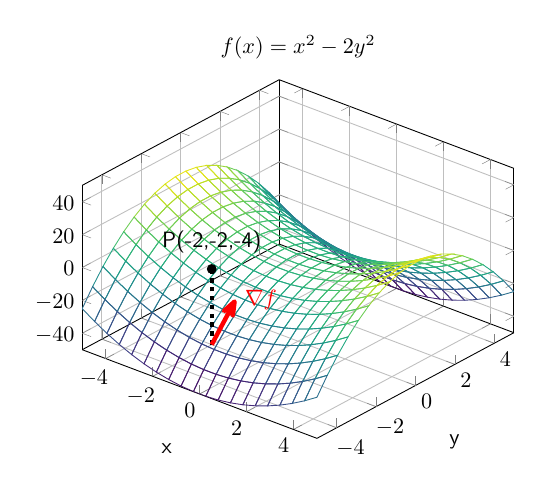
\begin{tikzpicture}[scale=0.8]
\usetikzlibrary {arrows.meta} 
\begin{axis}[
  colormap/viridis,  
  view = {40}{40},
	xmax = 5,
	xmin = -5,
	ymax = 5, 
	ymin = -5, 
	zmax = 50, 
	zmin = -50,
	xtick = {-4,-2,0,2,4},
	ytick = {-4,-2,0,2,4},
	ztick = {-40,-20,0,20,40},
	xlabel={x},
	ylabel={y},
	title={$f(x)=x^2-2y^2$},
	grid]
	

\addplot3 [
	domain=-5:5,
	domain y = -5:5,
	samples = 20,
	samples y = 20,
	mesh,
	%fill opacity=0.5,
	shader =faceted interp] {x^2 -2*y^2};
	
\draw[line width=2pt,dotted] (-2,-2,-50) -- (-2,-2,-4)	;
\node[label={P(-2,-2,-4)}] at (-2,-2,-4) {};
\draw plot [mark=*, mark size=2] coordinates{(-2,-2,-4)}; 
\draw[line width=2pt,red,-{Stealth[round]}] (-2,-2,-50)--(-3.5,1,-50) node[right]{$\nabla f$};

\end{axis}

\end{tikzpicture}
\captionof*{figure}{\textit{A vector parallel to the gradient vector is projected in the $xy$-plane. It points in the direction of most rapid increase.}}
}
%%%%%%%%%%%%%%%%%%%%%%%%%%%%%%%%



%%%%%%%%%%%%%%%%%%%%%%%%%%
\section{Integrals}
\label{sec:integrals}
\title{Integrals}
\institute{Mathmatical Tools and Their Use In Physics}
\author{\insertsubsection}
%%%%%%%%%%%%%%%%%%%%%%%%%%%%%%%%%%%


\begin{frame}
\titlepage
\thispagestyle{empty}
\end{frame}

%%%%%%%%%%%%%%%%%%%%%%%%%%%%%%%%%%%
\subsection{Rod examples}
\label{subsec:rodexamples}
\twocolframest{Example: The mass of a uniform rod}
{
\begin{itemize}
\scriptsize
\item Suppose that the rod has length L and mass M
\item We can define a linear mass density, $\mu$, (mass per unit length):
\begin{align*}
\mu=\frac{M}{L}
\end{align*}
\item A small section of rod, with length,$\Delta x$ , will have a mass:
\begin{align*}
\Delta m_i=\mu \Delta x
\end{align*}
\item<2-> We can think of the total rod of mass $M$, as the sum of $N$ identical ``mini rods'' of length, $\Delta x$ , each with mass, $\Delta m$ :
 \begin{align*}
 M=\sum_{i=0}^{i=N-1}\Delta m_i = \sum_{i=0}^{i=N-1} \mu \Delta x =\mu \sum_{i=0}^{i=N-1}\Delta x = \mu L
 \end{align*}
\end{itemize}
}
{
\centering
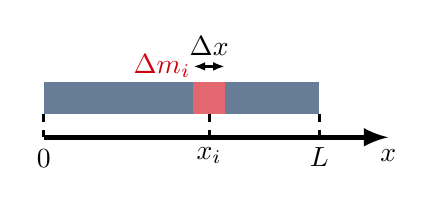
\begin{tikzpicture}[scale=1]
\tikzmath{
\L=3.5;
\w=0.4;
\h=0.3;
\dx=0.2;
}
\scalebox{1.0}{

\fill[myblue!60] (0,\h) rectangle (\L,\h+\w);

\draw[-latex, line width=2] (0,0) node[below] {$0$} -- (1.25*\L,0) node[below] {$x$};
\draw[dashed, line width=1] (0,\h) -- (0,0);
\draw[dashed, line width=1] (\L,\h) -- (\L,0) node[below] {$L$};

\draw[dashed, line width=1] (0.6*\L,\h) -- (0.6*\L,0) node[below] {$x_i$};

\fill[myred!60] (0.6*\L-\dx,\h) rectangle (0.6*\L+\dx,\h+\w);
\draw[{Latex[length=1.5mm]}-{Latex[length=1.5mm]},line width = 1] (0.6*\L-\dx,\h+\w+0.2) -- (0.6*\L+\dx,\h+\w+0.2)node[midway,above]{$\Delta x$};
\node[color=myred] at (0.6*\L-3*\dx,\h+\w+0.2){$\Delta m_i$};
}
\end{tikzpicture}
\captionof*{figure}{\textit{A rod of mass, $M$, and length, $L$, modeled as the sum of many ``mini rods'' of length $\Delta x$ and mass $\Delta m_i$.}}
}

%%%%%%%%%%%%%%%%%%%%%%%%%%%%%%%%
\twocolframest{Example: The mass of a \emph{non-uniform} rod}
{
\begin{itemize}
\scriptsize
\item Suppose the linear density \emph{varies} with position:
\begin{align*}
\mu = \mu(x)
\end{align*}
\item To get the mass of a length, $L$, of rod, we have to sum the masses of $N$ \emph{different} mini-rods:
\begin{align*}
\Delta m_i&=\mu(x_i) \Delta x\\
\therefore M &=\sum_{i=0}^{i=N-1}\Delta m_i =\lim_{\Delta x\to 0} \sum_{i=0}^{i=N-1} \mu(x_i) \Delta x
\end{align*}


\item How do we evaluate this sum? As $\Delta x\to 0$ , there are an infinite number of mini-rods (an infinite number of terms in the sum).
\item Keep in mind that this is the problem that we'd like to solve, as we go and get lost in math.
\end{itemize}
}
{
\centering
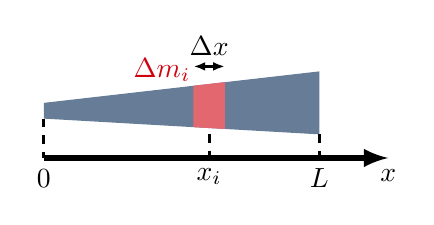
\begin{tikzpicture}[scale=1]
\tikzmath{
\L=3.5;
\w=0.4;
\h=0.3;
\dx=0.2;
\slobot=-\w/2/\L;
\ofsbot=\h+\w/2;
\slotop=\w/\L;
\ofstop=\h+\w;
\xmin=0.6*\L-\dx;
\yminbot=\slobot*\xmin+\ofsbot;
\ymintop=\slotop*\xmin+\ofstop;
\xmax=0.6*\L+\dx;
\ymaxbot=\slobot*\xmax+\ofsbot;
\ymaxtop=\slotop*\xmax+\ofstop;
}
\scalebox{1.0}{

\fill[myblue!60] (0,\h+\w/2) -- (\L,\h) -- (\L,\h+2*\w) -- (0,\h+\w);;

\draw[-latex, line width=2] (0,0) node[below] {$0$} -- (1.25*\L,0) node[below] {$x$};

\draw[dashed, line width=1] (0,\h+\w/2) -- (0,0);
\draw[dashed, line width=1] (\L,\h) -- (\L,0) node[below] {$L$};
\draw[dashed, line width=1] (0.6*\L,\h) -- (0.6*\L,0) node[below] {$x_i$};

\fill[myred!60] (\xmin,\yminbot) -- (\xmax,\ymaxbot) -- (\xmax,\ymaxtop) -- (\xmin,\ymintop);

\draw[{Latex[length=1.5mm]}-{Latex[length=1.5mm]},line width = 1] (\xmin,\ymaxtop+0.2) -- (\xmax,\ymaxtop+0.2)node[midway,above]{$\Delta x$};
\node[color=myred] at (0.6*\L-3*\dx,\ymintop+0.2){$\Delta m_i$};
}
\end{tikzpicture}
\captionof*{figure}{\textit{A non-uniform rod of mass, $M$, and length, $L$, modeled as the sum of many ``mini rods'' of length $\Delta x$ and mass $\Delta m_i$.}}
}


%%%%%%%%%%%%%%%%%%%%%%%%%%%%%%%%
\subsection{The anti-derivative}
\label{subsec:antider}
\begin{bulletframe}{The anti-derivative}
\item Tuesday, we saw that we can determine the rate of change of a function with respect to one (or more) of its independent variables (the derivative).
\item Today, we will see that given the derivative of a function, we can find the original function (the anti-derivative of the function that we are given).
\item Derivative of $f(x)$ with respect to $x$:  
\begin{align*}
f'(x) = \frac{d}{dx} f(x) \quad \text{Take the derivative with respect to x.}
\end{align*}
\item Anti-derivative of $f(x)$ with respect to $x$: 
\begin{align*}
F(x) &= \int f(x) dx \quad \text{Take the anti-derivative with respect to x.}\\
\therefore f(x) &= \frac{d}{dx} F(x)
\end{align*}

\end{bulletframe}


%%%%%%%%%%%%%%%%%%%%%%%%%%%%%%%%




%%%%%%%%%%%%%%%%%%%%%%%%%%%%%%%%
\twocolframest{The constant, $C$}
{

\begin{itemize}
\item Anti-derivatives are only determined up to a constant, $C$.
\item A synonym of anti-derivative is ``indefinite integral'' (since the function is not quite defined unless we specify $C$).
\item In physics, we need functions that describe physical quantities (say, your position along the x-axis as a function of time); those functions need to be fully defined (not up to some constant $C$).
\item The choice of the constant $C$ effectively chooses a point through which the function must pass.
\item It makes sense that the anti-derivative is not fully determined, since all of the functions on the right have the same derivative.
\end{itemize}

}
{
\centering
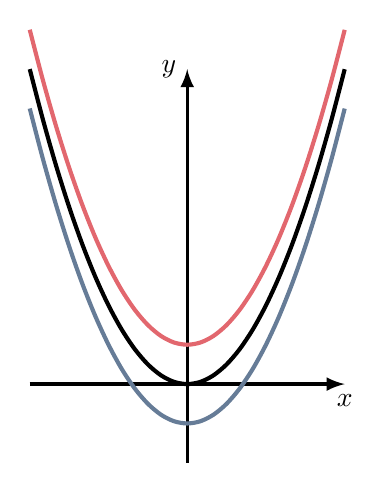
\begin{tikzpicture}[scale=1]
\tikzmath{
}
\scalebox{1.0}{
 
 \draw[-latex, line width=1.25pt] (-2,0) -- (2,0) node[below]{$x$}; 
 \draw[-latex, line width=1.25pt] (0,-1) -- (0,4) node[left]{$y$}; 
 
 %function
 \draw[scale=1, domain=-2.:2., smooth, variable=\x, line width=1.5,color=myblue!60] plot ({\x}, {\x*\x-0.5});
 \draw[scale=1, domain=-2.:2., smooth, variable=\x, line width=1.5] plot ({\x}, {\x*\x});
 \draw[scale=1, domain=-2.:2., smooth, variable=\x, line width=1.5,color=myred!60] plot ({\x}, {\x*\x+0.5});
}
\end{tikzpicture}
\captionof*{figure}{\textit{These functions, $f(x)=x^2+C$ all have the same derivative but different values of $C=\{-0.5,0,0.5\}$. }}
}


%%%%%%%%%%%%%%%%%%%%%%%%%%%%%%%%
\begin{bulletframe} {Determining the anti-derivative of a function} 
\item We would like to determine a function, $F(x)$, knowing:
\begin{itemize}
\item its derivative, $f(x)$.
\item the function must go through a specific point, say $(x_0,F_0)$.
\end{itemize}
\item Physics analogy: we would like to know the position of an object as a function of time, $x(t)$, knowing
\begin{itemize}
\item the velocity of the object as a function of time, $v(t)$ (the time derivative of the position):
\begin{align*}
v(t)=\frac{d}{dt} x(t)
\end{align*}
\item at time $t=t_0$, the object was located at a specific position:
\begin{align*}
x(t_0)=x_0
\end{align*}
\end{itemize}
\end{bulletframe}


%%%%%%%%%%%%%%%%%%%%%%%%%%%%%%%%
\twocolframesf{Graphically, how to visualize an anti-derivative}
{
\begin{itemize}
\item We know:
\begin{itemize}
\item the function $F(x)$ must go through a specific point, $(x_0,F_0)$ .
\item the derivative (slope) of the function at that point, $f(x_0)$.
\end{itemize}
\item<2-> We can determine the next point, $(x_1,F_1)$, through which the function should pass:
\begin{align*}
\frac{\Delta F}{\Delta x} &\approx f(x_0)\quad \text{becomes equal in the}\lim_{\Delta x \to 0}\\
\therefore \Delta F &\approx f(x_0)\Delta x\\
\therefore F_1 &\approx F_0+\Delta F =  F(x_0)+f(x_0)\Delta x
\end{align*}
\item<2->[$\rightarrow$] We now have a method to iterate and find all the points of $F(x)$.
\end{itemize}

}
{
\centering
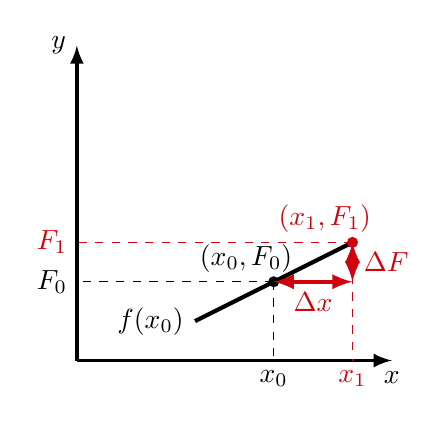
\begin{tikzpicture}[scale=1]
\tikzmath{
\xp=2.5;
\yp=1;
\dx=2;
}
\scalebox{1.0}{

 \coordinate (P) at (\xp,\yp);
 \coordinate (P1) at ($(P)+(\dx/2,0.5*\dx/2)$);
 
 
 \draw[-latex, line width=1.25pt] (0,0) -- (4,0) node[below]{$x$}; 
 \draw[-latex, line width=1.25pt] (0,0) -- (0,4) node[left]{$y$}; 
 
 \fill (P) circle(2pt);
 \node[left=10pt,above] at (P) { $(x_0,F_0)$};
 \draw[dashed] (P) -- +(0,-\yp) node[below]{$x_0$};
 \draw[dashed] (P) -- +(-\xp,0) node[left]{$F_0$};
 
 \draw[line width =1.5] ($(P)-(\dx/2,0.5*\dx/2)$) node[left] {$f(x_0)$} -- ($(P)+(\dx/2,0.5*\dx/2)$) ;
 \only<2->{
  \fill[color=myred] (P1) circle(2pt);
   \node[left=10pt,above,color=myred] at (P1) { $(x_1,F_1)$};
   \draw[dashed,color=myred] (P1) -- +(0,-\yp-0.5*\dx/2) node[below]{$x_1$};
   \draw[dashed,color=myred] (P1) -- +(-\xp-\dx/2,0) node[left]{$F_1$};
   \draw[latex-latex,line width =1.5, color=myred] (P1) -- +(0,-\dx/4) node[midway,right]{$\Delta F$};
   \draw[latex-latex,line width =1.5, color=myred] (P) -- +(\dx/2,0) node[midway,below]{$\Delta x$};
 }
 
}
\end{tikzpicture}
\captionof*{figure}{\textit{The ``shooting method'' for the anti-derivative.}}
}

%%%%%%%%%%%%%%%%%%%%%%%%%%%%%%%%



%%%%%%%%%%%%%%%%%%%%%%%%%%%%%%%%
\begin{bulletframe}{Extending the sum}
\item We have a procedure that allows us to determine the value of the function, $F(x)$, at any value of $x$ (say $x_N$ ):
\begin{align*}
F(x_N) = F(x_0)+f(x_0)\Delta x + f(x_1)\Delta x+ f(x_2)\Delta x+\dots + f(x_{N-1})\Delta x
\end{align*}
where $x_N=x_0+N\Delta x$
\item Using the summation notation and taking the limit:
\begin{align*}
F(x_N) = F(x_0)+\lim_{\Delta x \to 0}\sum_{i=0}^{N-1}f(x_i)\Delta x
\end{align*}
\end{bulletframe}


%%%%%%%%%%%%%%%%%%%%%%%%%%%%%%%%
\subsection{The indefinite and definite integrals}
\label{subsec:indefanddefintegrals}
\begin{bulletframe}{The indefinite and definite integrals}
\item We can re-write the sum as the difference in the anti-derivative evaluated at $x_N$ and $x_0$:
\begin{align*}
F(x_N) - F(x_0)=\lim_{\Delta x \to 0}\sum_{i=0}^{N-1}f(x_i)\Delta x
\end{align*}
The constant, $C$, in the anti-derivative cancels when we take this difference.
\item We call this difference the ``\textbf{definite integral (or just integral) of $f(x)$ from $x_0$  to $x_N$}'', and use the following notation:
\begin{align*}
\Aboxed{F(x_N) - F(x_0)=\int_{x_0}^{x_N}f(x)dx}
\end{align*}
\item Note the ``limits'' on the integral, which differentiates this from the anti-derivative.
\end{bulletframe}


%%%%%%%%%%%%%%%%%%%%%%%%%%%%%%%%
\begin{bulletframe}{Definite vs indefinite}
\item Given the function, $f(x)=x^2$
\item The indefinite integral (or anti-derivative) is a \textbf{function}:
\begin{align*}
F(x) = \int f(x) dx=\int x^2dx = \frac{1}{3}x^3+C
\end{align*}
\item The definite integral between $x=1$ and $x=3$ is a \textbf{number}:
\begin{align*}
\int_1^3x^2dx = F(3) - F(1) = \frac{1}{3}3^3-\frac{1}{3}1^3=9-\frac{1}{3}=\frac{26}{3}
\end{align*}
Note that the $C$ cancels in the subtraction.
\item Physical quantities in physics must be given by definite integrals.
\end{bulletframe}


%%%%%%%%%%%%%%%%%%%%%%%%%%%%%%%%
\subsection{How to determine the anti-derivative}
\label{subsec:determiningantider}
\twocolframe{How to determine the anti-derivative}
{
\begin{itemize}
\item To determine the anti-derivative of a function, $f(x)$, we need to be able to evaluate the sum:
\begin{align*}
\lim_{\Delta x \to 0}\sum_{i=0}^{N-1}f(x_i)\Delta x
\end{align*}
\item The textbook shows you how to do it for $f(x)=2x$. Your calculus course will show you how to do it for other functions...
\end{itemize}
}
{
\begin{center}
\scriptsize
\begin{tabular}{l l}
\textbf{Function, $f(x)$} & \textbf{Anti-derivative, $F(x)$}\\
\hline\hline
$f(x)=a$ & $F(x)=ax+C$ \\
$f(x)=x^n$ & $F(x)=\frac{1}{n+1}x^{n+1}+C$ \\
$f(x)=\frac{1}{x}$ & $F(x)=\ln(|x|)+C$ \\
$f(x)=\sin(x)$ & $F(x)=-\cos(x)+C$ \\
$f(x)=\cos(x)$ & $F(x)=\sin(x)+C$ \\
$f(x)=\tan(x)$ & $F(x)=-\ln(|\cos(x)|)+C$ \\
$f(x)=e^x$ & $F(x)=e^x+C$ \\
$f(x)=\ln(x)$ & $F(x)=x\ln(x)-x+C$ \\
\hline
\end{tabular}
\captionof*{table}{\label{tab:Calculus:commonints}Common indefinite integrals of functions. Unlike derivatives, for which you can always determine an analytical function, you cannot always determine an analytical form for the indefinite integral of a function. }
\end{center}
}



%%%%%%%%%%%%%%%%%%%%%%%%%%%%%%%%
%%%%%%%%%%%%%%%%%%%%%%%%%%%%%%%%
\twocolframesf{Graphical representation of the sum}
{
\scriptsize
\begin{itemize}
\item If we graph $f(x)$ we can see that each term in the sum for the integral corresponds to the area of a little rectangle under the function $f(x)$:
\begin{align*}
\lim_{\Delta x \to 0}\sum_{i=0}^{N-1}f(x_i)\Delta x = f(x_0)\Delta x + f(x_1)\Delta x\\
+ f(x_2)\Delta x+\dots + f(x_{N-1})\Delta x
\end{align*}
\item The definite integral:
\begin{align*}
\int_{x_0}^{X_N}f(x) dx=\lim_{\Delta x \to 0}\sum_{i=0}^{N-1}f(x_i)\Delta x 
\end{align*}
is thus the total area underneath $f(x)$, between $x_0$ and $x_N$  
\end{itemize}

}
{
\centering
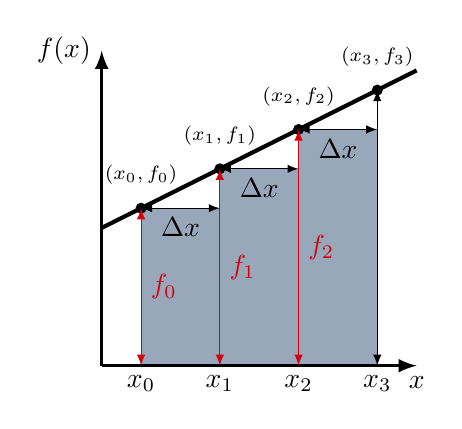
\begin{tikzpicture}[scale=1]
\tikzmath{
\xp=0.5;
\yp=2;
\dx=2;
}
\scalebox{1.0}{

 \coordinate (P) at (\xp,\yp);
 \coordinate (P1) at ($(P)+(\dx/2,0.5*\dx/2)$);
 \coordinate (P2) at ($(P)+2*(\dx/2,0.5*\dx/2)$);
 \coordinate (P3) at ($(P)+3*(\dx/2,0.5*\dx/2)$);
 
 \fill[color=myblue!40] (P) rectangle ($(P1)+(0,-\yp-0.5*\dx/2)$);
 \fill[color=myblue!40] (P1) rectangle ($(P2)+(0,-\yp-0.5*\dx)$);
 \fill[color=myblue!40] (P2) rectangle ($(P3)+(0,-\yp-0.75*\dx)$);
  
 
 \draw[-latex, line width=1.25pt] (0,0) -- (4,0) node[below]{$x$}; 
 \draw[-latex, line width=1.25pt] (0,0) -- (0,4) node[left]{$f(x)$}; 
 

 \draw[line width =1.5] ($(P)-0.5*(\dx/2,0.5*\dx/2)$)-- ($(P)+3.5*(\dx/2,0.5*\dx/2)$) ;
 
 \fill (P) circle(2pt);
 \draw[latex-latex,color=myred] (P) -- +(0,-\yp) node[below,color=black]{$x_0$} node[midway,right] {$f_0$};

 \fill (P1) circle(2pt);
 \draw[latex-latex,color=myred] (P1) -- +(0,-\yp-0.5*\dx/2) node[below,color=black]{$x_1$} node[midway,right] {$f_1$};

 \fill (P2) circle(2pt);
 \draw[latex-latex,color=myred] (P2) -- +(0,-\yp-0.5*\dx) node[below,color=black]{$x_2$} node[midway,right] {$f_2$};

 \fill (P3) circle(2pt);
 \draw[latex-latex] (P3) -- +(0,-\yp-0.75*\dx) node[below]{$x_3$} ;
 
 
 \draw[latex-latex] (P) -- +(\dx/2,0) node[midway,below] {$\Delta x$};
 \draw[latex-latex] (P1) -- +(\dx/2,0) node[midway,below] {$\Delta x$};
 \draw[latex-latex] (P2) -- +(\dx/2,0) node[midway,below] {$\Delta x$};

 \node[above=5pt] at (P) {\scriptsize $(x_0,f_0)$}; 
 \node[above=5pt] at (P1) {\scriptsize $(x_1,f_1)$};
 \node[above=5pt] at (P2) {\scriptsize $(x_2,f_2)$};
 \node[above=5pt] at (P3) {\scriptsize $(x_3,f_3)$};
 
}
\end{tikzpicture}
\captionof*{figure}{\textit{Each rectangle has an area $f(x_i) \Delta x$. As $\Delta x\to 0$, the rectangles correspond to the area under $f(x)$.}}
}



%%%%%%%%%%%%%%%%%%%%%%%%%%%%%%%%
%%%%%%%%%%%%%%%%%%%%%%%%%%%%%%%%
\subsection{Back to physiscs: the mass of a non-uniform rod}
\label{subsec:btpnonunirodmass}
\twocolframest{Back to physics: The mass of a \emph{non-uniform} rod}
{
\begin{itemize}
\scriptsize
\item Suppose the linear density \emph{varies} with position:
\begin{align*}
\mu = \mu(x)
\end{align*}
\item To get the mass of a length $L$ of rod, we have to sum the masses of $N$ \emph{different} mini-rods:
\begin{align*}
M &=\sum_{i=0}^{i=N-1}\Delta m_i =\lim_{\Delta x\to 0} \sum_{i=0}^{i=N-1} \mu(x_i) \Delta x
\end{align*}
\item The sum, is given by the definite integral:
\begin{align*}
\lim_{\Delta x\to 0} \sum_{i=0}^{i=N-1} \mu(x_i) \Delta x=\int_{x=0}^{x=L}\mu(x)dx
\end{align*}
If we know $\mu(x)$, we can ask our math friends for the anti-derivative of that function.
\end{itemize}

}
{
\begin{center}
\vspace{-1cm}
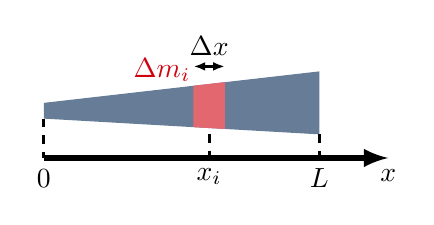
\begin{tikzpicture}[scale=1]
\tikzmath{
\L=3.5;
\w=0.4;
\h=0.3;
\dx=0.2;
\slobot=-\w/2/\L;
\ofsbot=\h+\w/2;
\slotop=\w/\L;
\ofstop=\h+\w;
\xmin=0.6*\L-\dx;
\yminbot=\slobot*\xmin+\ofsbot;
\ymintop=\slotop*\xmin+\ofstop;
\xmax=0.6*\L+\dx;
\ymaxbot=\slobot*\xmax+\ofsbot;
\ymaxtop=\slotop*\xmax+\ofstop;
}
\scalebox{1.0}{

\fill[myblue!60] (0,\h+\w/2) -- (\L,\h) -- (\L,\h+2*\w) -- (0,\h+\w);;

\draw[-latex, line width=2] (0,0) node[below] {$0$} -- (1.25*\L,0) node[below] {$x$};

\draw[dashed, line width=1] (0,\h+\w/2) -- (0,0);
\draw[dashed, line width=1] (\L,\h) -- (\L,0) node[below] {$L$};
\draw[dashed, line width=1] (0.6*\L,\h) -- (0.6*\L,0) node[below] {$x_i$};

\fill[myred!60] (\xmin,\yminbot) -- (\xmax,\ymaxbot) -- (\xmax,\ymaxtop) -- (\xmin,\ymintop);

\draw[{Latex[length=1.5mm]}-{Latex[length=1.5mm]},line width = 1] (\xmin,\ymaxtop+0.2) -- (\xmax,\ymaxtop+0.2)node[midway,above]{$\Delta x$};
\node[color=myred] at (0.6*\L-3*\dx,\ymintop+0.2){$\Delta m_i$};
}
\end{tikzpicture}
\captionof*{figure}{\textit{A non-uniform rod of mass, $M$, and length, $L$, modeled as the sum of many ``mini rods'' of length $\Delta x$ and mass $\Delta m_i$.}}
\end{center}
\only<2>{
\scriptsize
\color{myblue!60}{As physicists, we need a tool to be able to calculate these sums.\\
The mathematicians (well actually...) have developed this tool from calculus that can find the anti-derivative of a function.\\
It turns out that this tool also gives a way to calculate the sums that we need in physics!}
}
}


%%%%%%%%%%%%%%%%%%%%%%%%%%%%%%%%
\begin{frame}{Back to physics: The mass of a \emph{non-uniform} rod}
\begin{itemize}
\item Suppose that $\mu(x)=2ax$, then we (our math friends) know that:
\begin{align*}
F(x) = \int \mu(x) dx = ax^2+C
\end{align*}
\item We want:
\begin{align*}
\lim_{\Delta x\to 0} \sum_{i=0}^{i=N} \mu(x_i) \Delta x=\int_{x=0}^{x=L}\mu(x)dx
\end{align*}
\item We can thus evaluate:
\begin{align*}
\int_{x=0}^{x=L}\mu(x)dx = F(x=L)-F(x=0) = aL^2 - 0 = aL^2
\end{align*}
\end{itemize}
\end{frame}


%%%%%%%%%%%%%%%%%%%%%%%%%%%%%%%%
\twocolframest{The infinitesimals}
{
\begin{itemize}
\scriptsize
\item We can think of an \textit{infinitesimally small} rod of mass, $dm$, and length, $dx$:
\begin{align*}
dm = \mu(x) dx
\end{align*}
\item The total mass of the rod, $M$, is the sum of the masses of the infinitesimal rods:
\begin{align*}
M = \sum dm = \int_0^M dm= \int_0^L\mu(x) dx
\end{align*}
\item With practice, you will get used to just writing everything with infinitesimals rather than a sum and taking the limits!
\item This also makes it clear that \textbf{an integral is a sum}
\end{itemize}

}
{
\vspace{-1cm}
\begin{center}

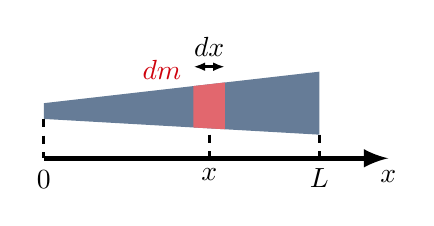
\begin{tikzpicture}[scale=1]
\tikzmath{
\L=3.5;
\w=0.4;
\h=0.3;
\dx=0.2;
\slobot=-\w/2/\L;
\ofsbot=\h+\w/2;
\slotop=\w/\L;
\ofstop=\h+\w;
\xmin=0.6*\L-\dx;
\yminbot=\slobot*\xmin+\ofsbot;
\ymintop=\slotop*\xmin+\ofstop;
\xmax=0.6*\L+\dx;
\ymaxbot=\slobot*\xmax+\ofsbot;
\ymaxtop=\slotop*\xmax+\ofstop;
}
\scalebox{1.0}{

\fill[myblue!60] (0,\h+\w/2) -- (\L,\h) -- (\L,\h+2*\w) -- (0,\h+\w);;

\draw[-latex, line width=2] (0,0) node[below] {$0$} -- (1.25*\L,0) node[below] {$x$};

\draw[dashed, line width=1] (0,\h+\w/2) -- (0,0);
\draw[dashed, line width=1] (\L,\h) -- (\L,0) node[below] {$L$};
\draw[dashed, line width=1] (0.6*\L,\h) -- (0.6*\L,0) node[below] {$x$};

\fill[myred!60] (\xmin,\yminbot) -- (\xmax,\ymaxbot) -- (\xmax,\ymaxtop) -- (\xmin,\ymintop);

\draw[{Latex[length=1.5mm]}-{Latex[length=1.5mm]},line width = 1] (\xmin,\ymaxtop+0.2) -- (\xmax,\ymaxtop+0.2)node[midway,above]{$dx$};
\node[color=myred] at (0.6*\L-3*\dx,\ymintop+0.2){$dm$};
}
\end{tikzpicture}
\captionof*{figure}{\textit{A non-uniform rod of mass, $M$, and length, $L$, modeled as the sum of many ``mini rods'' of length $\Delta x$ and mass $\Delta m_i$.}}
\end{center}
\scriptsize
Compare with:
\begin{align*}
\Delta m_i &= \mu(x) \Delta x\\
M &=\sum_{i=0}^{i=N}\Delta m_i 
=\lim_{\Delta x\to 0} \sum_{i=0}^{i=N-1} \mu(x_i) \Delta x
\end{align*}
}


%%%%%%%%%%%%%%%%%%%%%%%%%%%%%%%%



%%%%%%%%%%%%%%%%%%%%%%%%%%%%%%%%



%%%%%%%%%%%%%%%%%%%%%%%%%%%%%%%%



%%%%%%%%%%%%%%%%%%%%%%%%%%%%%%%%



%%%%%%%%%%%%%%%%%%%%%%%%%%%%%%%%



%%%%%%%%%%%%%%%%%%%%%%%%%%%%%%%%



%%%%%%%%%%%%%%%%%%%%%%%%%%%%%%%%



%%%%%%%%%%%%%%%%%%%%%%%%%%%%%%%%



%%%%%%%%%%%%%%%%%%%%%%%%%%%%%%%%











\title{Kinematics}
\subject{1D, nD and Circular Motion}
\subtitle{Building Models to Describe our World}


%%%%%%%%%%%%%%%%%%%%%%%%%%%%%%
%%%%%%%%%%%%%%%%%%%%%




%%%%%%%%%%%%%%%%%%%%%%%%%
%%%%%% Title slide %%%%%%
%%%%%%%%%%%%%%%%%%%%%%%%%
\chaptertitle{Kinematics}
\begin{frame}
\label{chap:kinematics}
\titlepage
\thispagestyle{empty}

\begin{textblock*}{5cm}(11cm,4cm)
    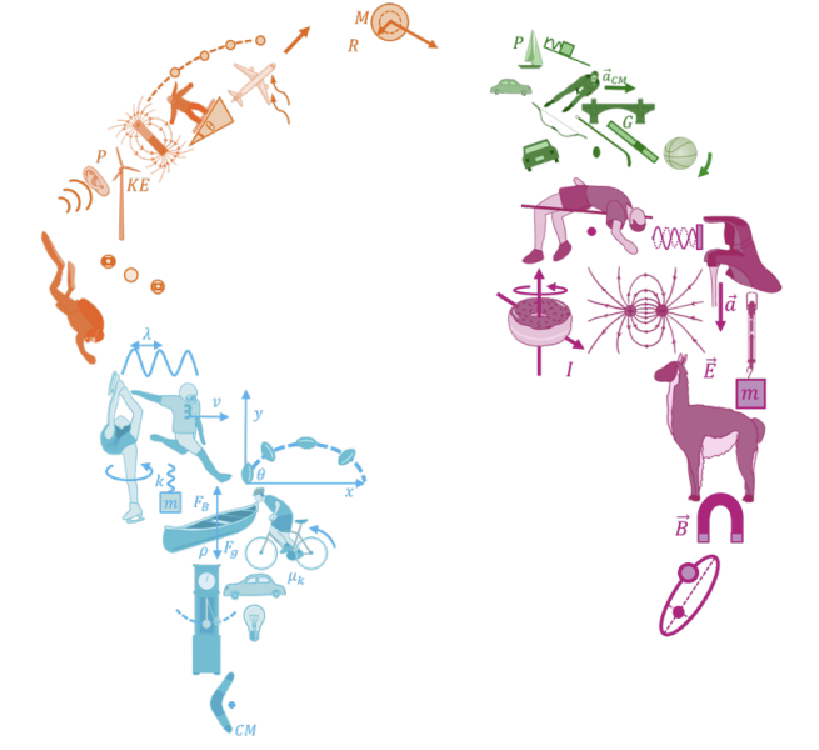
\includegraphics[width=4cm]{figures/BMDW/logo}
\end{textblock*}

\end{frame}

%%%%%%%%%%%%%TOC
\twocolframe{Outline}
  {\tableofcontents[sections={7,8}, subsectionstyle=show/show]\thispagestyle{empty}}
  {\tableofcontents[sections={9}, subsectionstyle=show/show]}
%%%%%%%%%%%%%%%%%%%%%%%%%







%%%%%%%%%%%%%%%%%%%%%%%%%%%%%%%%
\section{1D Kinematics}
\label{sec:1dkinematics}
\title{Kinematics in One Dimension}


%%%%%%%%%%%%%%%%%%%%%%%%%
\begin{frame}
\titlepage
\thispagestyle{empty}
\end{frame}

%%%%%%%%%%%%%%%%%%%%%%%%






%%%%%%%%%%%%%%%%%%%%%%%%%%%%%%%%
\subsection{Velocity and speed basics}
\label{subsec:velocityandspeedbasics}
\twocolframesf{Average vs instantaneous velocity/speed}
{
\begin{itemize}
\item Velocity is a measure of the rate of change of position.
\item Velocity is positive(negative) if position is increasing(decreasing).
\item Speed is the magnitude of velocity.
\item \textbf{Average velocity}:
\begin{align*}
v=\frac{\Delta x}{\Delta t}
\end{align*}
\item<2-> \textbf{Instantaneous velocity} at some point in time:
\begin{align*}
v=\lim_{\Delta t \to 0}\frac{\Delta x}{\Delta t}=\frac{dx}{dt}
\end{align*}
\end{itemize}
}
{
\centering
\begin{tikzpicture}[%
%https://tex.stackexchange.com/questions/25928/how-to-draw-tangent-line-of-an-arbitrary-point-on-a-path-in-tikz
        tangent/.style={
        decoration={
            markings,% switch on markings
            mark=
                at position ####1
                with
                {
                    \coordinate (tangent point-\pgfkeysvalueof{/pgf/decoration/mark info/sequence number}) at (0pt,0pt);
                    \coordinate (tangent unit vector-\pgfkeysvalueof{/pgf/decoration/mark info/sequence number}) at (1,0pt);
                    \coordinate (tangent orthogonal unit vector-\pgfkeysvalueof{/pgf/decoration/mark info/sequence number}) at (0pt,1);
                }
        },
        postaction=decorate
    },
    use tangent/.style={
        shift=(tangent point-####1),
        x=(tangent unit vector-####1),
        y=(tangent orthogonal unit vector-####1)
    },
    use tangent/.default=1
    ]

\scalebox{1.0}{

 \coordinate (P1) at (0,0.5);
 \coordinate (P2) at (1.75,2); %used to make the path squiggly
 \coordinate (P3) at (3.75,2.5);
 \coordinate (P3x) at ($(0,0)!(P3)!(1,0)$);
 \coordinate (P1P3) at ($(P3)!(P1)!(P3x)$);
 
 \draw[-latex, line width=1.25pt] (0,0) -- (4.5,0) node[below]{$t$}; 
 \draw[-latex, line width=1.25pt] node[below]{\SI{0}{min}} (0,0) -- (0,3) node[left]{$x$}; 
 
 \fill (P1) circle(2pt);
 \fill (P3) circle(2pt);
 
 %The path with tangent coordinates calculated
 \draw[tangent=0.1,tangent=0.4, line width=1pt] (P1) to [out=10,in=190] (P2) to [out=10,in=260] (P3);
 
 \node[left] at (P1) {\SI{100}{km}};
 \draw[dashed] (P3) -- ($(0,0)!(P3)!(0,1)$) node[left] {\SI{150}{km}};
 \draw[dashed] (P3) -- (P3x) node[below] {\SI{30}{min}};
 \draw[dashed] (P1) -- (P1P3) ;
 
 \only<1>{
 \draw[latex-latex,color=myred,line width=1.5pt] (P3) -- (P1P3) node[midway,left]{$\Delta x$};
 \draw[latex-latex,color=myred,line width=1.5pt] (P1) -- (P1P3) node[midway,above]{$\Delta t$};
 }
 
 
 \only<2>{
 \draw [myred, line width=1.5, use tangent=1] (-0.5,0) -- (0.5,0) node[right]{$v=\frac{dx}{dt}$};
 \draw [myred, line width=1.5, use tangent=2] (-0.5,0) -- (0.5,0) node[left]{$v=\frac{dx}{dt}$};
 }
 

}
\end{tikzpicture}
\only<1>{
\captionof*{figure}{\textit{Position as a function of time. Average velocity is the total displacement divided by the total time.}}
}
\only<2>{
\captionof*{figure}{\textit{Position as a function of time. Instantaneous velocity is the derivative at any given point.}}
}
}


%%%%%%%%%%%%%%%%%%%%%%%%%%%%%%%%




%%%%%%%%%%%%%%%%%%%%%%%%%%%%%%%
\subsection{Acceleration}
\label{subsec:acceleration}
\begin{bulletframe}{Acceleration}
\item Acceleration is the rate of change of velocity
\item Average acceleration :
\begin{align*}
a=\frac{\Delta v}{\Delta t}
\end{align*}
\item Instantaneous acceleration at some point in time:
\begin{align*}
a(t)&=\lim_{\Delta t \to 0}\frac{\Delta v}{\Delta t}=\frac{dv}{dt}\\
\therefore v(t) &= \int a(t) dt
\end{align*}
\end{bulletframe}


%%%%%%%%%%%%%%%%%%%%%%%%%%%%%%%%

\begin{bulletframe}{The kinematic equations for constant acceleration}
\scriptsize
\item<1-> If the acceleration is constant:
\begin{align*}
a(t) &= a\\
\therefore v(t) &= \int adt = at+C
\end{align*}
\item<2-> The constant $C$ can be determined from knowing that, say, at $t=0$, $v=v_0$:
\begin{align*}
v(t=0)&=a(0)+C = v_0\\
\therefore C&=v_0\\
\Aboxed{\therefore v(t)&= v_0 + at}
\end{align*}
\item<3-> Since velocity is the time-derivative of position, $x(t)$, position is the anti-derivative of velocity:
\begin{align*}
x(t)=\int v(t) dt = \int (at+v_0) dt = \frac{1}{2}at^2+v_0 t+C'
\end{align*}
\item<4-> Again, we can determine the second integration constant, $C'=x_0$, if we know that $x =x_0$  at $t=0$:
\begin{align*}
\Aboxed{ x(t) = \frac{1}{2}at^2+v_0 t+x_0}
\end{align*}
\end{bulletframe}


%%%%%%%%%%%%%%%%%%%%%%%%%%%%%%%%
\subsection{Group activity: kinematics scetching}
\label{subsec:grpactivitykinematics}
\twocolframe{Group question}
{
Using the following graph of $a(t)$, sketch out the corresponding $v(t)$ and $x(t)$. \textbf{Assume that, at $t=0$, the position is negative and that the speed is positive.}
}
{


\centering
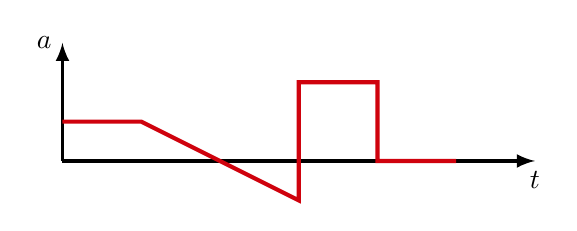
\begin{tikzpicture}[scale =1]

\scalebox{1.0}{

 \coordinate (P1) at (0,0.5);
 \coordinate (P2) at (1,0.5); %used to make the path squiggly
 \coordinate (P3) at (2,0);
 \coordinate (P4) at (3,-0.5);
 \coordinate (P5) at (3,1);
 \coordinate (P6) at (4,1);
 \coordinate (P7) at (4,0);
 \coordinate (P8) at (5,0);
 \coordinate (P1x) at ($(0,0)!(P1)!(1,0)$);
 \coordinate (P2x) at ($(0,0)!(P2)!(1,0)$);
 \coordinate (P3x) at ($(0,0)!(P3)!(1,0)$);
 \coordinate (P4x) at ($(0,0)!(P4)!(1,0)$);
 \coordinate (P5x) at ($(0,0)!(P5)!(1,0)$);
 
 \draw[-latex, line width=1.25pt] (0,0) -- (6,0) node[below]{$t$}; 
 \draw[-latex, line width=1.25pt] (0,0) -- (0,1.5) node[left]{$a$}; 
 
 
 \draw[line width =1.5pt,color=myred] (P1) -- (P2) -- (P3) -- (P4) -- (P5) -- (P6) -- (P7) -- (P8);
 

}
\end{tikzpicture}

\captionof*{figure}{\textit{Acceleration as a function of time.}}

}

%%%%%%%%%%%%%%%%%%%%%%%%%%%%%%%%

\twocolframe{Velocity, $v(t)$}
{
\begin{enumerate}
\item Acceleration is constant and positive, velocity increases linearly.
\item Acceleration is decreasing to zero, velocity increases less and less
\item Acceleration becomes more negative, velocity increases in the negative direction more and more
\item Acceleration is constant and positive, velocity increases linearly.
\item Acceleration is zero, velocity is constant.
\end{enumerate}
}
{

\centering
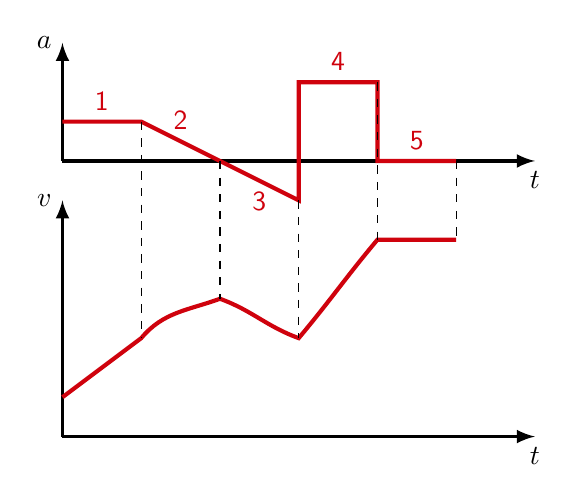
\begin{tikzpicture}[scale =1]
\tikzmath{
\ysh=-3.5;
}

\scalebox{1.0}{

 \coordinate (P1) at (0,0.5);
 \coordinate (P2) at (1,0.5); %used to make the path squiggly
 \coordinate (P3) at (2,0);
 \coordinate (P4) at (3,-0.5);
 \coordinate (P5) at (3,1);
 \coordinate (P6) at (4,1);
 \coordinate (P7) at (4,0);
 \coordinate (P8) at (5,0);
 \coordinate (P1x) at ($(0,0)!(P1)!(1,0)$);
 \coordinate (P2x) at ($(0,0)!(P2)!(1,0)$);
 \coordinate (P3x) at ($(0,0)!(P3)!(1,0)$);
 \coordinate (P4x) at ($(0,0)!(P4)!(1,0)$);
 \coordinate (P5x) at ($(0,0)!(P5)!(1,0)$);
 
 %a
 \draw[-latex, line width=1.25pt] (0,0) -- (6,0) node[below]{$t$}; 
 \draw[-latex, line width=1.25pt] (0,0) -- (0,1.5) node[left]{$a$}; 
 
 \draw[line width =1.5pt,color=myred] (P1) -- (P2) node[midway,above]{1} -- (P3)  node[midway,above]{2}-- (P4) node[midway,below]{3} -- (P5)  -- (P6)  node[midway,above]{4}-- (P7)  -- (P8) node[midway,above]{5};
 
 %vaxis
 \draw[-latex, line width=1.25pt] (0,\ysh) -- (6,\ysh) node[below]{$t$}; 
 \draw[-latex, line width=1.25pt] (0,\ysh) -- (0,\ysh+3) node[left]{$v$}; 
 
 \coordinate (P1V) at (0,\ysh+0.5);
 \coordinate (P2V) at (1,\ysh+1.25);
 \coordinate (P3V) at (2,\ysh+1.75);
 \coordinate (P4V) at (3,\ysh+1.25);
 \coordinate (P5V) at (3,\ysh+0.5);
 \coordinate (P6V) at (4,\ysh+2.5);
 \coordinate (P7V) at (4,\ysh+0.5);
 \coordinate (P8V) at (5,\ysh+2.5);
 
 \draw[line width =1.5pt,color=myred] (P1V) to (P2V) [out=50,in=200] to (P3V) [out=340,in=160] to (P4V) [out=50,in=230]  to (P6V) [out=0,in=180] to (P8V) ;

 \draw[dashed] (P2) -- (P2V);
 \draw[dashed] (P3) -- (P3V);
 \draw[dashed] (P4) -- (P4V);
 \draw[dashed] (P6) -- (P6V);
 \draw[dashed] (P8) -- (P8V);
 
}
\end{tikzpicture}

\captionof*{figure}{\textit{Velocity from acceleration, the object always goes in the positive direction}}

}

%%%%%%%%%%%%%%%%%%%%%%%%%%%%%%%%

\twocolframe{Position, $x(t)$}
{
\begin{enumerate}
\item Velocity increases linearly, position increase quadratically
\item Velocity increases less and less, position increases less than quadratically
\item Positive velocity decreases, position decreases less than quadratically.
\item Velocity increases linearly, position increase quadratically
\item Velocity is constant, position increases linearly
\end{enumerate}
}
{

\centering
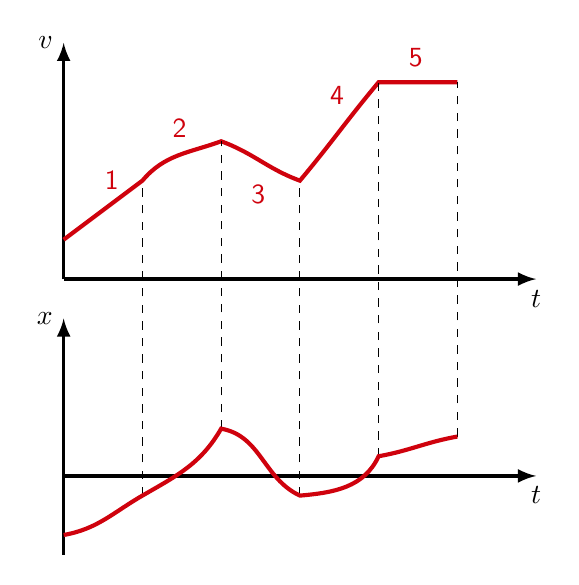
\begin{tikzpicture}[scale =1]
\tikzmath{
\ysh=0;
\xsh=-2.5;
}

\scalebox{1.0}{

 
 %vaxis
 \draw[-latex, line width=1.25pt] (0,\ysh) -- (6,\ysh) node[below]{$t$}; 
 \draw[-latex, line width=1.25pt] (0,\ysh) -- (0,\ysh+3) node[left]{$v$}; 
 
 \coordinate (P1V) at (0,\ysh+0.5);
 \coordinate (P2V) at (1,\ysh+1.25);
 \coordinate (P3V) at (2,\ysh+1.75);
 \coordinate (P4V) at (3,\ysh+1.25);
 %\coordinate (P5V) at (3,\ysh+0.5);
 \coordinate (P6V) at (4,\ysh+2.5);
 %\coordinate (P7V) at (4,\ysh+0.5);
 \coordinate (P8V) at (5,\ysh+2.5);
 
 \draw[line width =1.5pt,color=myred] (P1V) to (P2V) [out=50,in=200] to (P3V) [out=340,in=160] to (P4V) [out=50,in=230]  to (P6V) [out=0,in=180] to (P8V) ;

 %xaxis
 \draw[-latex, line width=1.25pt] (0,\xsh) -- (6,\xsh) node[below]{$t$}; 
 \draw[-latex, line width=1.25pt] (0,\xsh-1) -- (0,\xsh+2) node[left]{$x$}; 


 \coordinate (P1X) at (0,\xsh-0.75);
 \coordinate (P2X) at (1,\xsh-0.25);
 \coordinate (P3X) at (2,\xsh-0.+0.6);
 \coordinate (P4X) at (3,\xsh-0.25);
 \coordinate (P6X) at (4,\xsh+0.25);
 \coordinate (P8X) at (5,\xsh+0.5);

 \draw[dashed] (P2X) -- (P2V);
 \draw[dashed] (P3X) -- (P3V);
 \draw[dashed] (P4X) -- (P4V);
 \draw[dashed] (P6X) -- (P6V);
 \draw[dashed] (P8X) -- (P8V);
 
 \draw[line width =1.5pt,color=myred] (P1X) to [out=10,in=210] (P2X) to [out=30, in=240] (P3X) to [out=-10, in=155] (P4X) to [out=5, in=245] (P6X) to [out=10, in=190] (P8X);
 
 \node[left=5pt,color=myred] at (P2V) {1};
 \node[left=15pt,above=-2pt,color=myred] at (P3V) {2};
 \node[left=15pt,below=-2pt,color=myred] at (P4V) {3};
 \node[left=15pt,below=-2pt,color=myred] at (P6V) {4};
 \node[left=15pt,above=2pt,color=myred] at (P8V) {5};
 
% 
}
\end{tikzpicture}

\captionof*{figure}{\textit{Position from velocity}}

,}
%%%%%%%%%%%%%%%%%%%%%%%%%%%%

\subsection{Relative motion notation in 1D}
\label{subsec:relmotionnotation1d}
\twocolframest{1D Relative motion - notation}
{
\begin{itemize}
\item We can think of different ``frames of reference'', i.e. different coordinate systems that move relative to each other
\item We choose to use primes (‘) to denote quantities in one frame of reference, and letters to identify the object:
\begin{align*}
\textcolor{myred}{v^{'A}}=\textcolor{myblue}{v^{'B}}+v^A
\end{align*}
\end{itemize}


In words:\textcolor{myred}{The velocity of Alice as measured in the prime reference frame (Igor, the ground)} \textcolor{myblue}{is the velocity of Brice (the train) measured relative to the ground} plus \textbf{the velocity of Alice measured relative to the un-primed reference frame} (aka Brice).
}
{
\capfig{1}{figures/Kinematics/trainABC}{Igor watches a train with Brice (sitting) and Alice (walking) in it.}
Same idea with position:
\begin{align*}
\textcolor{myred}{x^{'A}}&=\textcolor{myblue}{x^{'B}}+x^A\\
\textcolor{myred}{x^{'A}}&=\textcolor{myblue}{v^{'B}t}+x^A
\end{align*}
}





%%%%%%%%%%%%%%%%%%%%%%%%%%%%


\section{nD Kinematics}
\label{sec:ndkinematics}
\title{Kinematics in Multiple Dimensions}
\institute{Mathmatical Tools and Their Use In Physics}
\author{\insertsubsection}


%%%%%%%%%%%%%%%%%%%%%%%%%
\begin{frame}
\titlepage
\thispagestyle{empty}
\end{frame}
%%%%%%%%%%%%%%%%%%%%%%%%%%















%%%%%%%%%%%%%%%%%%%%%%%%%%%%%
\subsection{2D motion}
\label{subsec:2dmotion}
\begin{bulletframe}{2D motion}
\item Same as 1D, but we need to describe both of the x and y coordinates of the object
\item The most compact notation to do this is to use vectors
\item Position:
\begin{align*}
\vec r (t) = \begin{pmatrix}
x(t)\\y(t)
\end{pmatrix}
\end{align*}
By specifying the vector,$\vec r (t)$ , relative to the origin of an $xy$ coordinate system, we fully specify the position of an object (namely its $x$ and $y$ coordinates as a function of time.
\end{bulletframe}



%%%%%%%%%%%%%%%%%%%%%%%%%%%%%%%%
\subsection{Relative motion notation in 2D}
\label{subsec:relmotionnotation2d}
\twocolframest{2D Relative motion - notation}
{
\begin{itemize}
\item We can think of different ``frames of reference'', i.e. different coordinate systems that move relative to each other
\item We choose to use primes (‘) to denote quantities in one frame of reference, and letters to identify the object:
\begin{align*}
\textcolor{myred}{\vec v^{'A}}=\textcolor{myblue}{\vec v^{'B}}+\vec v^A
\end{align*}
\end{itemize}


In words:\textcolor{myred}{The velocity of Alice as measured in the prime reference frame (Igor, the ground)} \textcolor{myblue}{is the velocity of Brice (the train) measured relative to the ground} plus \textbf{the velocity of Alice measured relative to the un-primed reference frame} (aka Brice).
}
{
\capfig{1}{figures/Kinematics/trainABC}{Igor watches a train with Brice (sitting) and Alice (walking) in it.}
Same idea with position:
\begin{align*}
\textcolor{myred}{\vec r^{'A}}&=\textcolor{myblue}{\vec r^{'B}}+\vec r^A\\
\textcolor{myred}{\vec r^{'A}}&=\textcolor{myblue}{\vec v^{'B}t}+\vec r^A
\end{align*}
}



%%%%%%%%%%%%%%%%%%%%%%%%%%%%%%%%


%%%%%%%%%%%%%%%%%%%%%%%%%%%%%%%%
\subsection{Building a model: feed the monkey!}
\label{subsec:buildingmodelmonkey}
\twocolframesf{Feeding the monkey: building a model}
{
$\rightarrow$ How do we throw the banana in order for the monkey to catch it? The monkey will let go of the branch as soon as we throw the banana.
}
{
\capfig{1}{figures/Kinematics/MonkeyTreeExample}{As soon as the banana is released, the monkey lets go of the branch. How to throw the banana for the monkey to catch it?}
}


%%%%%%%%%%%%%%%%%%%%%%%%%%%%%%%%
\twocolframesf{Start with initial conditions}
{
\begin{itemize}
\item We choose a coordinate system $\rightarrow$ in this case: origin at starting position of banana, $y$ positive up, $x$ positive right
\item We have 2 objects, the banana and the monkey, whose motion we want to describe:
\begin{align*}
\vec r_b(t), \vec r_m(t)
\end{align*}
\item At time $t=0$, they have initial position and velocity vectors:
\begin{align*}
\vec r_{b0}, \vec r_{m0}, \textcolor{myred}{\vec v_{b0}}, \vec v_{m0}
\end{align*}
\item We want to determine $\textcolor{myred}{\vec v_{b0}}$, the initial velocity of the banana
\end{itemize}
}
{
\capfig{1}{figures/Kinematics/MonkeyTreeExample}{As soon as the banana is released, the monkey lets go of the branch. How to throw the banana for the monkey to catch it?}
\begin{tikzpicture}[remember picture,overlay]%
 \draw[-latex, line width=2, color=myred] ($(current page.center)+(2.3,-0.55)$) -- +(1.5,0.625) node[above]{$\vec v_{b0}$} ;%
 \draw[line width =1.5, color=myred] ($(current page.center)+(3.1,-0.55)$) arc (0:22.6:0.8) node[midway,right] {$\theta$};
\end{tikzpicture}
}


%%%%%%%%%%%%%%%%%%%%%%%%%%%%%%%%




%%%%%%%%%%%%%%%%%%%%%%%%%%%%%%%%
\twocolframesf{Equate the positions of the banana and monkey}
{\scriptsize
\begin{itemize}
\item For constant acceleration:
\begin{align*}
\vec r(t) = \vec r_0 + \vec v_0 t + \frac{1}{2} \vec a t^2
\end{align*}
\item<2-> For the banana, $\vec r_{b0}=0$, this gives:
\begin{align*}
\vec r_b (t) = v_{b0} \begin{pmatrix}
\cos\theta \\ \sin\theta
\end{pmatrix}
t+ \frac{1}{2} \begin{pmatrix}
0\\ \SI{-9.8}{m/s^2}
\end{pmatrix}t^2
\end{align*}
\item<3-> For the monkey, $\vec v_{m0}=0$, this gives:
\begin{align*}
\vec r_m (t) = \begin{pmatrix}
d \\ h
\end{pmatrix}
+ \frac{1}{2} \begin{pmatrix}
0\\ \SI{-9.8}{m/s^2}
\end{pmatrix}t^2
\end{align*}

\end{itemize}
}
{\scriptsize
\begin{itemize}
\item<4-> The positions must be the same at some time $t$, $\vec r_b (t)=\vec r_m (t)$, writing this out for each component:
\begin{align*}
v_{b0}\cos\theta t&= d\\
v_{b0}\sin\theta t-\frac{1}{2}(\SI{9.8}{m/s^2}) t^2&= h-\frac{1}{2}(\SI{9.8}{m/s^2})t^2
\end{align*}
\item<5-> Simplify:
\begin{align*}
v_{b0}\cos\theta t&= d\\
v_{b0}\sin\theta t&= h
\end{align*}
\item<6> Divide one equation by the other to eliminate $t, v_{b0}$ and get $\theta$:
\begin{align*}
\frac{\sin\theta}{\cos \theta}=\Aboxed{\tan\theta=\frac{h}{d}}
\end{align*}
\end{itemize}
}

%%%%%%%%%%%%%%%%%%%%%%%%%%%%%%%%
\twocolframesf{Thinking about the model, $\tan\theta=\frac{h}{d}$}
{
\begin{itemize}
\item This is somewhat surprising; all we have to do is aim for the monkey...
\item The speed at which we throw the banana does not matter!
\item If we throw the banana faster, it will intercept the monkey higher above the ground.
\item Think of this in the absence of gravity (then you obviously aim for the monkey) – in the presence of gravity, both the banana and monkey move downwards by the same amount in the same amount of time, $\textcolor{myred}{\frac{1}{2}gt^2}$
\end{itemize}
}
{
\capfig{1}{figures/Kinematics/MonkeyTreeExample}{As soon as the banana is released, the monkey lets go of the branch. How to throw the banana for the monkey to catch it? Just aim for the monkey!}
\begin{tikzpicture}[remember picture,overlay]%
 \draw[-latex, line width=2, color=myred] ($(current page.center)+(2.3,-0.55)$) -- +(1.5,0.625) node[above]{$\vec v_{b0}$} ;%
 \draw[line width=0.75, dashed, color=myred] ($(current page.center)+(2.3,-0.55)$) -- +(3,1.25) ;%
 \draw[line width =1.5, color=myred] ($(current page.center)+(3.1,-0.55)$) arc (0:22.6:0.8) node[midway,right] {$\theta$};
\end{tikzpicture}
}
%%%%%%%%%%%%%%%%%%%%%%%%%%%%%%%%%%%%%%%5

\subsection{Zeno's paradox}
\label{subsec:zenosparadox}
\begin{frame}{Zeno's paradox}
An example of Zeno's paradox: If you shoot an arrow at speed, $v$, towards a target a distance, $D$, away, it must first cover half the distance. After that, it must still go the other half, so it travels half of that remaining distance. If you think of it this way, like Zeno, you appear to have a different paradox, the arrow can never get there because there is always a small distance left. Any motion is thus impossible!

\end{frame}

\twocolframesf{Zeno's arrow: Kinematics to the rescue!}
{
\begin{itemize}
\item At constant speed, $v$, it will take a time, $T$, for the arrow to cover the distance, $D$:
\begin{align*}
T=\frac{D}{v}
\end{align*}
\item The time that it will take to cover the first, second, third segments:
\begin{align*}
t_1=\frac{D}{2v}\quad t_2=\frac{D}{4v}\quad t_3=\frac{D}{8v}\;\; \dots \;\; t_N=\frac{D}{2vN}
\end{align*}
\item The total time is thus also given by:
\begin{align*}
T=t_1+t_2+t_3+\dots=\sum_{i=1}^N t_i=\frac{D}{v}\sum_{1=1}^N\frac{1}{2i}
\end{align*}

\end{itemize}
}
{
\vspace{-1.5cm}
\begin{center}
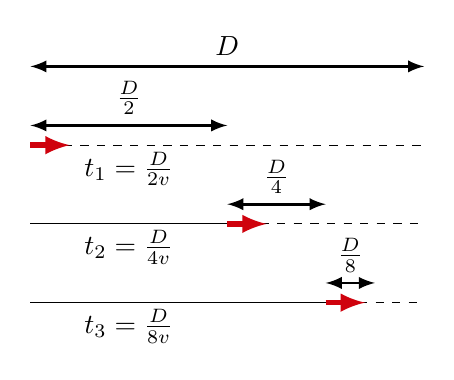
\begin{tikzpicture}[scale=1]
\tikzmath{
\L=5;
\h=1;
\lv=0.5;
}
\scalebox{1.0}{
%\draw[line width=2] (0,0) -- (\L,0);
\draw[latex-latex,line width=1] (0,0) -- (\L,0) node[midway,above]{$D$};
%\fill (0,0) circle (2pt);
%\fill (\L,0) circle (2pt);

\draw[dashed] (0,-\h) -- +(\L,0);
\draw[latex-latex,line width=1] (0,-\h+0.25) -- +(\L/2,0) node[midway,above]{$\frac{D}{2}$};
\draw[-latex,line width=2, color=myred] (0,-\h)--+(\lv,0);
\node at (\L/4,-\h-0.3){$t_1=\frac{D}{2v}$};

\draw[dashed] (\L/2,-2*\h) -- +(\L/2,0);
\draw[latex-latex,line width=1] (\L/2,-2*\h+0.25) -- +(\L/4,0) node[midway,above]{$\frac{D}{4}$};
\draw[](0,-2*\h) -- +(\L/2,0);
\draw[-latex,line width=2, color=myred] (\L/2,-2*\h)--+(\lv,0);
\node at (\L/4,-2*\h-0.3){$t_2=\frac{D}{4v}$};

\draw[dashed] (3*\L/4,-3*\h) -- +(\L/4,0);
\draw[latex-latex,line width=1] (3*\L/4,-3*\h+0.25) -- +(\L/8,0) node[midway,above]{$\frac{D}{8}$};
\draw[](0,-3*\h) -- +(3*\L/4,0);
\draw[-latex,line width=2, color=myred] (3*\L/4,-3*\h)--+(\lv,0);
\node at (\L/4,-3*\h-0.3){$t_3=\frac{D}{8v}$};
}
\end{tikzpicture}
\captionof*{figure}{\textit{An arrow traveling Zeno's way!}}
\end{center}
\vspace{-0.5cm}
\only<2>{
\begin{block}{Resolving the paradox:}
The two ways of calculating, $T$, must be equivalent, thus:
\begin{align*}
\lim_{N\to\infty}\sum_{1=1}^N\frac{1}{2i} = 1
\end{align*}
The geometric series converges!
\end{block}
}
}

%%%%%%%%%%%%%%%%%%%%%%












%%%%%%%%%%%%%%%%%%%%%%%%%%%%%%%%
\section{Circular Motion}
\label{sec:circularmotion}
\title{Circular Motion}
\institute{Mathmatical Tools and Their Use In Physics}
\author{\insertsubsection}


%%%%%%%%%%%%%%%%%%%%%%%%%
\begin{frame}
\titlepage
\thispagestyle{empty}
\end{frame}


%%%%%%%%%%%%%%%%%%%%%%%%%%%%%%%%














%%%%%%%%%%%%%%%%%%%%%%%%%%%%%%%%
\subsection{Acceleration with constant speed}
\label{subsec:accelerationwithconstantspeed}
\twocolframesf{Acceleration vector: constant speed}
{
\begin{itemize}
\item The acceleration vector of an object is non-zero if the velocity vector changes.
\item[$\rightarrow$] The velocity vector can change magnitude, direction,\textit{ or both}!
\item<2> For constant speed, the acceleration vector is perpendicular to the velocity vector, in the limit of $\Delta t\to 0$ (as we'll see). 
\end{itemize}
}
{
\begin{center}
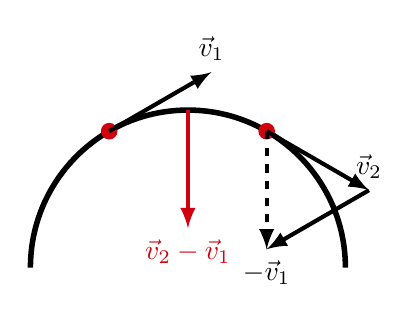
\begin{tikzpicture}[scale=1]
\tikzmath{
\R=2;
\th=30;
\Px=\R*sin(\th);
\Py=\R*cos(\th);
\v=1.5;
\vx=\v*cos(\th);
\vy=\v*sin(\th);
}
\scalebox{1.0}{

\coordinate (P1) at (-\Px,\Py);
\coordinate (P2) at (\Px,\Py);

\draw[line width=2] (\R,0) arc(0:180:\R);
\fill[color=myred] (P1) circle(3pt);
\fill[color=myred] (P2) circle(3pt);

\draw[-latex,line width =1.5] (P1) -- +(\vx,\vy) node[above]{$\vec v_1$};
\draw[-latex,line width =1.5] (P2) -- +(\vx,-\vy) node[above]{$\vec v_2$};

\only<2>{
\draw[-latex,line width =1.5] ($(P2)+(\vx,-\vy)$) -- +(-\vx,-\vy) node[below ]{$-\vec v_1$};
\draw[-latex,dashed,line width =1.5] (P2) -- ($(P2)+(0,-2*\vy)$) ;
\draw[-latex,line width =1.5,color=myred] (0,\R) -- +(0,-2*\vy) node[below] {$\vec v_2-\vec v_1$};
}

}
\end{tikzpicture}
\only<1>{\captionof*{figure}{\textit{Velocity vector of an object going around a circle.}}}
\only<2>{\captionof*{figure}{\textit{The change in velocity vector $ \Delta\vec v=\vec v_2-\vec v_1$ is perpendicular to the trajectory.}}}
\end{center}

}

\subsection{Taking the derivative of a vector}
\label{subsec:takingthederivativeofavector}
%%%%%%%%%%%%%%%%%%%%%%%%%%%%%%%%
\begin{bulletframe}{Taking the derivative of a vector}
\item The average acceleration vector is defined as:
\begin{align*}
\vec a = \frac{\Delta \vec v}{\Delta t}
\end{align*}
\item Dividing a vector by a scalar (divide each component):
\begin{align*}
\begin{pmatrix}
a_x\\a_y
\end{pmatrix}
= \begin{pmatrix}
\frac{\Delta v_x}{\Delta t}\\
\frac{\Delta v_y}{\Delta t}
\end{pmatrix}
\end{align*}
\item The instantaneous acceleration is given by taking $\Delta t \to 0$:
 \begin{align*}
 \vec a = \frac{d}{dt}\vec v=
\begin{pmatrix}
a_x\\a_y
\end{pmatrix}
= \begin{pmatrix}
\frac{d v_x}{dt}\\
\frac{d v_y}{dt}
\end{pmatrix}
\end{align*}
\end{bulletframe}


%%%%%%%%%%%%%%%%%%%%%%%%%%%%%%%%


%%%%%%%%%%%%%%%%%%%%%%%%%%%%%%%%
%%%%%%%%%%%%%%%%%%%%%%%%%%%%%%%%
\subsection{The acceleration vector}
\label{subsec:theaccelerationvector}
\twocolframesf{Acceleration vector: general case}
{
\begin{itemize}
\item In general, the velocity vector can change both magnitude and direction.
\item The acceleration vector, $\vec a$, will, in general, have components that are perpendicular and parallel to the instantaneous velocity:
\begin{itemize}
\item You can think of the \textcolor{myred}{perpendicular component}, $\vec a_\perp$, as being responsible for the \textcolor{myred}{change in direction}.
\item You can think of \textcolor{blue}{the parallel component}, $\vec a_\parallel$, as being responsible for the \textcolor{blue}{change in speed}
\end{itemize}
\end{itemize}
}
{
\begin{center}
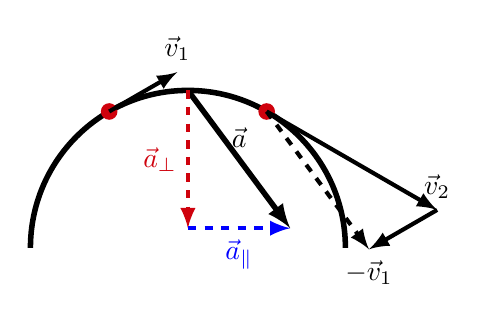
\begin{tikzpicture}[scale=1]
\tikzmath{
\R=2;
\th=30;
\Px=\R*sin(\th);
\Py=\R*cos(\th);
\v=1;
\vx=\v*cos(\th);
\vy=\v*sin(\th);
\vv=2.5;
\vvx=\vv*cos(\th);
\vvy=\vv*sin(\th);
}
\scalebox{1.0}{

\coordinate (P1) at (-\Px,\Py);
\coordinate (P2) at (\Px,\Py);

\draw[line width=2] (\R,0) arc(0:180:\R);
\fill[color=myred] (P1) circle(3pt);
\fill[color=myred] (P2) circle(3pt);

\draw[-latex,line width =1.5] (P1) -- +(\vx,\vy) node[above]{$\vec v_1$};
\draw[-latex,line width =1.5] (P2) -- +(\vvx,-\vvy) node[above]{$\vec v_2$};


\draw[-latex,line width =1.5] ($(P2)+(\vvx,-\vvy)$) -- +(-\vx,-\vy) node[below ]{$-\vec v_1$};
\draw[-latex,dashed,line width =1.5] (P2) -- ($(P2)+(\vvx-\vx,-\vvy-\vy)$) ;
\draw[-latex,line width =2] (0,\R) -- +(\vvx-\vx,-\vvy-\vy) node[midway,above] {$\vec a$};
\draw[-latex,dashed, line width =1.5,color=myred] (0,\R) -- +(0,-\vvy-\vy) node[midway,left] {$\vec a_{\perp}$};
\draw[-latex,dashed, line width =1.5,color=blue] ($(0,\R)+(0,-\vvy-\vy)$) -- +(\vvx-\vx,0) node[midway,below] {$\vec a_{\parallel}$};
}
\end{tikzpicture}
\captionof*{figure}{\textit{The acceleration has a component perpendicular to the trajectory due to the direction changing, and a component parallel due to the magnitude changing.}}
\end{center}

}

%%%%%%%%%%%%%%%%%%%%%%%%%%%

\subsection{Describing motion around a circle}
\label{subsec:describingmotionaroundacircle}
\twocolframesf{Motion along a circle}
{
\begin{itemize}
\item We wish to describe the motion of an object moving along a circular path.
\item This is 2D motion, but constrained along a (1D) line.
\item We have several ways to describe the motion:
\begin{itemize}
\item Using full 2D description, $\vec r(t)$. 
\item Using a 1D description along a curved axis: $s(t)$.
\item Using a 1D description using angular quantities: $\theta(t)$.
\end{itemize}
\item They are, of course, all related and equivalent.
\item 1D is usually more convenient!
\end{itemize}
}
{
\begin{center}
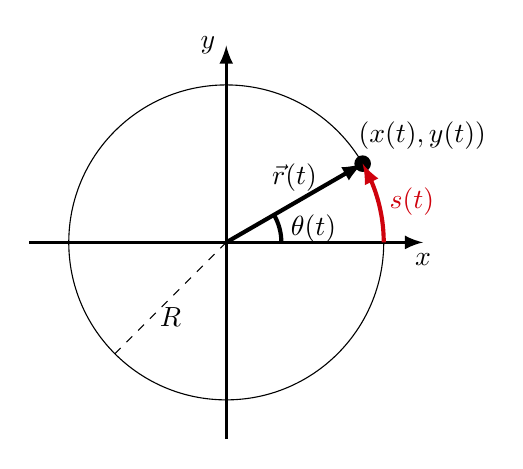
\begin{tikzpicture}[scale=1]
\tikzmath{
\R=2;
\th=30;
\Px=\R*cos(\th);
\Py=\R*sin(\th);
}
\scalebox{1.0}{

\coordinate (P) at (\Px,\Py);

\draw[-latex, line width=1.25pt] (-1.25*\R,0) -- (1.25*\R,0) node[below]{$x$}; 
\draw[-latex, line width=1.25pt] (0,-1.25*\R) -- (0,1.25*\R) node[left]{$y$};

\draw (0,0) circle (\R); 
\fill (P) circle(3pt);
\draw[-latex, line width = 1.5] (0,0) -- (P) node[midway,above] {$\vec r(t)$};
\draw[line width = 1.5] (0.7,0) arc (0:\th:0.7) node[midway,right]{$\theta(t)$};
\draw[-latex, color=myred, line width = 1.5] (\R,0) arc (0:\th:\R) node[midway,right]{$s(t)$};
\node[above=10pt, right=-5pt] at (P) {$\left(x(t),y(t)\right)$};
\draw[dashed] (0,0) --+(225:\R) node[midway,below]{$R$};

}
\end{tikzpicture}
\captionof*{figure}{\textit{Different ways to describe motion around a circle.}}
\end{center}

}


%%%%%%%%%%%%%%%%%%%%%%%%%%%%%%%%

%%%%%%%%%%%%%%%%%%%%%%%%%%%%%%%%
\begin{bulletframe}{Angular velocity and angular acceleration}
\item<1-> The rate of change of the angle (angular velocity):
\begin{align*}
\omega = \frac{d\theta}{dt}
\end{align*}
\item<1-> The rate of change of the angular velocity (angular acceleration)
\begin{align*}
\alpha = \frac{d\omega}{dt}
\end{align*}
\item<2-> For \textbf{constant angular acceleration}, we have (from taking anti-derivatives):
\begin{align*}
\omega(t) &= \omega_0 + \alpha t\\
\theta(t) &= \theta_0+\omega t+\frac{1}{2}\alpha t^2
\end{align*}
If the object was located at $\theta =\theta_0$, with angular velocity, $\omega_0$, at time $t=0$
\end{bulletframe}


%%%%%%%%%%%%%%%%%%%%%%%%%%%%%%%%

%%%%%%%%%%%%%%%%%%%%%%%%%%%%%%%%
\twocolframesf{Relating $\theta(t)$ and $s(t)$}
{\scriptsize
\begin{itemize}
\item The angular position:
\begin{align*}
\theta(t)=\frac{1}{R} s(t)
\end{align*}
\item<2-> The angular velocity:
\begin{align*}
\omega(t)=\frac{d}{dt} \left(\frac{1}{R}s(t)\right)=\frac{1}{R}\frac{ds}{dt}=\frac{1}{R}v_s
\end{align*}
\item<2-> The angular acceleration:
\begin{align*}
\alpha(t)=\frac{d}{dt} \left(\frac{1}{R}v_s(t)\right)=\frac{1}{R}\frac{dv_s}{dt}=\frac{1}{R}a_s
\end{align*}
\item<2-> The ``linear'' or ``tangential'' ($s,v_s,a_s$) and angular ($\theta,\omega,\alpha$) quantities are connected by the radius $R$:
\begin{align*}
\text{linear quantity}=R\times\text{angular quantity}
\end{align*}
\end{itemize}
}
{
\begin{center}
\vspace{-1cm}
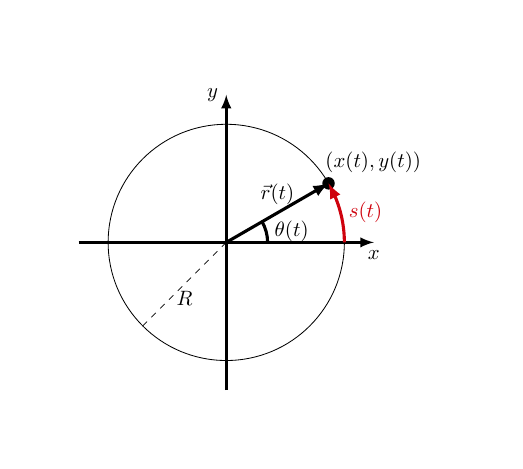
\begin{tikzpicture}[scale=1]
\tikzmath{
\R=2;
\th=30;
\Px=\R*cos(\th);
\Py=\R*sin(\th);
}
\scalebox{0.75}{

\coordinate (P) at (\Px,\Py);

\draw[-latex, line width=1.25pt] (-1.25*\R,0) -- (1.25*\R,0) node[below]{$x$}; 
\draw[-latex, line width=1.25pt] (0,-1.25*\R) -- (0,1.25*\R) node[left]{$y$};

\draw (0,0) circle (\R); 
\fill (P) circle(3pt);
\draw[-latex, line width = 1.5] (0,0) -- (P) node[midway,above] {$\vec r(t)$};
\draw[line width = 1.5] (0.7,0) arc (0:\th:0.7) node[midway,right]{$\theta(t)$};
\draw[-latex, color=myred, line width = 1.5] (\R,0) arc (0:\th:\R) node[midway,right]{$s(t)$};
\node[above=10pt, right=-5pt] at (P) {$\left(x(t),y(t)\right)$};
\draw[dashed] (0,0) --+(225:\R) node[midway,below]{$R$};

}
\end{tikzpicture}
\end{center}
\vspace{-1cm}
\only<2>{
\begin{align*}
\Aboxed{s(t)&=R\theta(t)}\\
\Aboxed{v_s(t)&=R\omega(t)}\\
\Aboxed{a_s(t)&=R\alpha(t)}
\end{align*}
}
}


%%%%%%%%%%%%%%%%%%%%%%%%%%%%%%%%
\twocolframesf{Vector description for circular motion}
{
\begin{itemize}
\item Velocity from position:
\begin{align*}
\vec r &= R \begin{pmatrix}
\cos\left(\theta(t)\right)\\
\sin\left(\theta(t)\right)
\end{pmatrix}\\
\therefore \vec v &= \frac{d}{dt} \vec r=\frac{d}{dt} R \begin{pmatrix}
\cos\left(\theta(t)\right)\\
\sin\left(\theta(t)\right)
\end{pmatrix}\\
&=R \begin{pmatrix}
\frac{d}{dt}\cos\left(\theta(t)\right)\\
\frac{d}{dt}\sin\left(\theta(t)\right)
\end{pmatrix}
=R \begin{pmatrix}
-\sin\left(\theta(t)\right)\frac{d\theta}{dt}\\
\cos\left(\theta(t)\right)\frac{d\theta}{dt}
\end{pmatrix}\\
&=R\omega\begin{pmatrix}
-\sin\left(\theta(t)\right)\\
\cos\left(\theta(t)\right)
\end{pmatrix}
\end{align*}

\end{itemize}
Velocity and position are perpendicular. The velocity is tangent to the circle, as expected. The magnitude of the velocity vector is $v=v_s=\omega R$.
}
{
\begin{center}
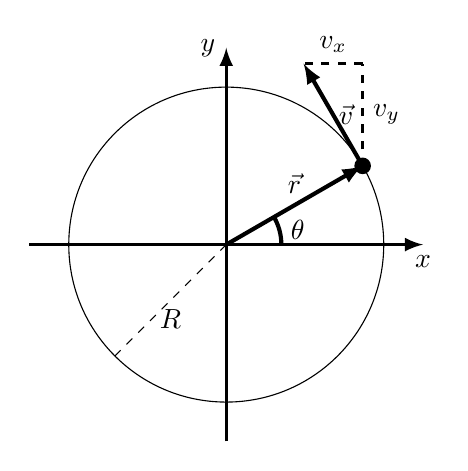
\begin{tikzpicture}[scale=1]
\tikzmath{
\R=2;
\th=30;
\Px=\R*cos(\th);
\Py=\R*sin(\th);
\v=1.5;
\vx=-\v*sin(\th);
\vy=\v*cos(\th);
}
\scalebox{1}{

\coordinate (P) at (\Px,\Py);

\draw[-latex, line width=1.25pt] (-1.25*\R,0) -- (1.25*\R,0) node[below]{$x$}; 
\draw[-latex, line width=1.25pt] (0,-1.25*\R) -- (0,1.25*\R) node[left]{$y$};

\draw (0,0) circle (\R); 
\fill (P) circle(3pt);
\draw[-latex, line width = 1.5] (0,0) -- (P) node[midway,above] {$\vec r$};
\draw[line width = 1.5] (0.7,0) arc (0:\th:0.7) node[midway,right]{$\theta$};
\draw[-latex, line width = 1.5] (P) -- +(\vx,\vy) node[midway,right=-2pt] {$\vec v$};
\draw[dashed, line width = 1.] (P) -- +(0,\vy) node[midway,right] {$v_y$};
\draw[dashed, line width = 1.] ($(P) +(0,\vy)$) -- +(\vx,0) node[midway,above] {$v_x$};

\draw[dashed] (0,0) --+(225:\R) node[midway,below]{$R$};

}
\end{tikzpicture}
\end{center}

}


%%%%%%%%%%%%%%%%%%%%%%%%%%%%%%%%
\twocolframesf{Vector description for circular motion}
{\scriptsize
\begin{itemize}
\item The linear velocity, $v_s$, is the magnitude of the velocity vector:
\begin{align*}
\vec v &= R\omega\begin{pmatrix}
-\sin\left(\theta(t)\right)\\
\cos\left(\theta(t)\right)
\end{pmatrix}=v_s(t)\begin{pmatrix}
-\sin\left(\theta(t)\right)\\
\cos\left(\theta(t)\right)
\end{pmatrix}\\
\therefore ||\vec v||&=v=v_s=R\omega
\end{align*}
\item The direction of the velocity vector is given by:
\begin{align*}
\hat v = \begin{pmatrix}
-\sin\left(\theta(t)\right)\\
\cos\left(\theta(t)\right)
\end{pmatrix}
\end{align*}
which is a unit vector (length of 1).
\item We can write the velocity vector as:
\begin{align*}
\vec v =v(t) \hat v(t)
\end{align*}
\end{itemize}
The direction of the velocity vector, $\hat v$, changes with time, and the magnitude, $v$, could change with time.
}
{
\begin{center}
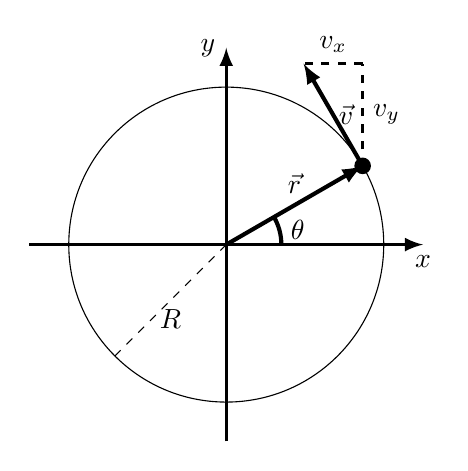
\begin{tikzpicture}[scale=1]
\tikzmath{
\R=2;
\th=30;
\Px=\R*cos(\th);
\Py=\R*sin(\th);
\v=1.5;
\vx=-\v*sin(\th);
\vy=\v*cos(\th);
}
\scalebox{1}{

\coordinate (P) at (\Px,\Py);

\draw[-latex, line width=1.25pt] (-1.25*\R,0) -- (1.25*\R,0) node[below]{$x$}; 
\draw[-latex, line width=1.25pt] (0,-1.25*\R) -- (0,1.25*\R) node[left]{$y$};

\draw (0,0) circle (\R); 
\fill (P) circle(3pt);
\draw[-latex, line width = 1.5] (0,0) -- (P) node[midway,above] {$\vec r$};
\draw[line width = 1.5] (0.7,0) arc (0:\th:0.7) node[midway,right]{$\theta$};
\draw[-latex, line width = 1.5] (P) -- +(\vx,\vy) node[midway,right=-2pt] {$\vec v$};
\draw[dashed, line width = 1.] (P) -- +(0,\vy) node[midway,right] {$v_y$};
\draw[dashed, line width = 1.] ($(P) +(0,\vy)$) -- +(\vx,0) node[midway,above] {$v_x$};

\draw[dashed] (0,0) --+(225:\R) node[midway,below]{$R$};

}
\end{tikzpicture}
\end{center}

}


%%%%%%%%%%%%%%%%%%%%%%%%%%%%%%%%
\subsection{Deriving the acceleration vector}
\label{subsec:deriveaccvector}
\begin{frame}{Acceleration for circular motion}
\begin{itemize}
\item<1-> The acceleration vectors is given by:
\begin{align*}
\vec a = \frac{d}{dt} \vec v = \frac{d}{dt} \textcolor{blue}{v(t)} \textcolor{myred}{\hat v (t)}
\end{align*}
\item<2-> Use the product rule for derivatives:
\begin{align*}
\vec a = \textcolor{blue}{\frac{dv}{dt} \hat v (t)}+ \textcolor{myred}{v(t)\frac{d\hat v}{dt} }
\end{align*}
\item<3-> Part of the acceleration vector is due to \textcolor{blue}{change in speed, $\frac{dv}{dt}$, and is \textbf{parallel} to the velocity, $\hat v$}, and part is due to \textcolor{myred}{change in direction, $\frac{d\hat v}{dt}$ and in a \textbf{different direction}}:
\begin{align*}
\vec a = \textcolor{blue}{a_s \hat v (t)}+ \textcolor{myred}{v(t)\frac{d}{dt} \begin{pmatrix}
-\sin\left(\theta(t)\right)\\
\cos\left(\theta(t)\right)
\end{pmatrix}}
\end{align*}
\end{itemize}

\end{frame}


%%%%%%%%%%%%%%%%%%%%%%%%%%%%%%%%
\begin{frame}{The change in direction}
\begin{itemize}
\item<1-> Apply the Chain Rule (again) to obtain the change in direction:
\begin{align*}
\textcolor{myred}{\frac{d\hat v}{dt}}=
\textcolor{myred}{\frac{d}{dt} \begin{pmatrix}
-\sin\left(\theta(t)\right)\\
\cos\left(\theta(t)\right)
\end{pmatrix}} = \textcolor{myred}{ \begin{pmatrix}
-\cos\left(\theta(t)\right)\frac{d\theta}{dt}\\
-\sin\left(\theta(t)\right)\frac{d\theta}{dt}
\end{pmatrix}} = \textcolor{myred}{\omega \begin{pmatrix}
-\cos\left(\theta(t)\right)\\
-\sin\left(\theta(t)\right)\end{pmatrix}}
\end{align*}
\item<2-> Note that this is perpendicular to the velocity ($\hat v$) and has magnitude of $\omega$. The vector $\textcolor{myred}{\frac{d\hat v}{dt}}$ points towards the centre of the circle.
\end{itemize}
\only<2>{
\vspace{-0.75cm}
\begin{center}
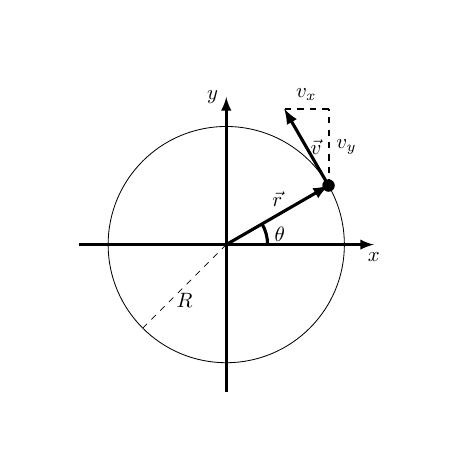
\begin{tikzpicture}[scale=1]
\tikzmath{
\R=2;
\th=30;
\Px=\R*cos(\th);
\Py=\R*sin(\th);
\v=1.5;
\vx=-\v*sin(\th);
\vy=\v*cos(\th);
}
\scalebox{0.75}{

\coordinate (P) at (\Px,\Py);

\draw[-latex, line width=1.25pt] (-1.25*\R,0) -- (1.25*\R,0) node[below]{$x$}; 
\draw[-latex, line width=1.25pt] (0,-1.25*\R) -- (0,1.25*\R) node[left]{$y$};

\draw (0,0) circle (\R); 
\fill (P) circle(3pt);
\draw[-latex, line width = 1.5] (0,0) -- (P) node[midway,above] {$\vec r$};
\draw[line width = 1.5] (0.7,0) arc (0:\th:0.7) node[midway,right]{$\theta$};
\draw[-latex, line width = 1.5] (P) -- +(\vx,\vy) node[midway,right=-2pt] {$\vec v$};
\draw[dashed, line width = 1.] (P) -- +(0,\vy) node[midway,right] {$v_y$};
\draw[dashed, line width = 1.] ($(P) +(0,\vy)$) -- +(\vx,0) node[midway,above] {$v_x$};

\draw[dashed] (0,0) --+(225:\R) node[midway,below]{$R$};

}
\end{tikzpicture}
\end{center}
}
\end{frame}


%%%%%%%%%%%%%%%%%%%%%%%%%%%%%%%%
\begin{frame}{Finally}
\begin{itemize}
\item The acceleration vector is given by:
\begin{align*}
\vec a = \textcolor{blue}{a_s \hat v (t)}+ \textcolor{myred}{v(t)\omega \begin{pmatrix}
-\cos\left(\theta(t)\right)\\
-\sin\left(\theta(t)\right)\end{pmatrix}}=\textcolor{blue}{\alpha(t) R\hat v (t)}+ \textcolor{myred}{\omega^2(t) R \begin{pmatrix}
-\cos\left(\theta(t)\right)\\
-\sin\left(\theta(t)\right)\end{pmatrix}}
\end{align*}
where we used the relations $v(t)=\omega(t) R$ and $a_s(t)=\alpha(t) R$.
\item It has two components:
\begin{enumerate}
\item A \textcolor{blue}{component \textbf{tangent to the circle} (parallel to velocity)}, \textbf{if the speed changes} (``tangential'' acceleration), with magnitude:
\begin{align*}
a_s=a_\parallel=a_T=\frac{dv}{dt}=R\alpha
\end{align*}
\item A \textcolor{myred}{component \textbf{towards the center of the circle} (perpendicular to velocity)} \textbf{because the velocity changes direction} (``centripetal'' or ``radial'' acceleration), with magnitude:
\begin{align*}
a_c=a_\perp=a_R=\omega^2 R=\frac{v^2}{R}
\end{align*}
\end{enumerate}
\end{itemize}
\end{frame}


%%%%%%%%%%%%%%%%%%%%%%%%%%%%%%%%



%%%%%%%%%%%%%%%%%%%%%%%%%%%%%%%%



%%%%%%%%%%%%%%%%%%%%%%%%%%%%%%%%



%%%%%%%%%%%%%%%%%%%%%%%%%%%%%%%%



%%%%%%%%%%%%%%%%%%%%%%%%%%%%%%%%



%%%%%%%%%%%%%%%%%%%%%%%%%%%%%%%%





































%%%%%%%%%%%%%%%%%%%%%%%%%%%%%%%%

\title{Newton's Laws}
\subject{Newton, Forces, and Free Body Diagrams}
\subtitle{Building Models to Describe our World}


\chaptertitle{Newton's Laws}
\begin{frame}
\label{chap:newtonslaws}
\titlepage
\thispagestyle{empty}

\begin{textblock*}{5cm}(11cm,4cm)
    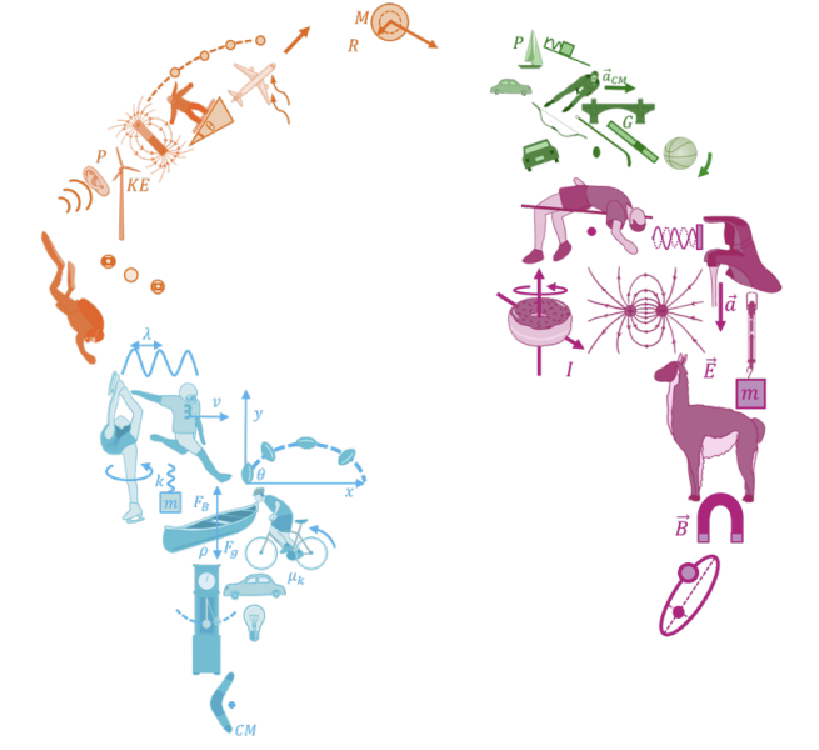
\includegraphics[width=4cm]{figures/BMDW/logo}
\end{textblock*}

\end{frame}

%%%%%%%%%%%%%%%%%

\twocolframe{Outline}
{\tableofcontents[sections=10-11, subsectionstyle=show/show]\thispagestyle{empty}}
{\tableofcontents[sections=12, subsectionstyle=show/show]}

%%%%%%%%%%%%%%%%%%%

\section{Concepts}
\label{sec:newtonsconcepts}
\title{Concepts}
\institute{Newton's Laws}
\author{\insertsubsection}

%%%%%%%%%%%%


\begin{frame}
\titlepage
\thispagestyle{empty}
\end{frame}

%%%%%%%%%%%%%%%%%%

\subsection{What is a force?}
\label{subsec:forces}
\begin{bulletframe}{What is a force?}
\item There is no such thing as a force.
\item These are a mathematical tool that allows us to describe the motion of objects. 
\item We represent them with a vector, as they have a magnitude and a direction.
\item We can use a spring scale to define the magnitude and direction of a force.
\item One issue is that we have some intuition about what a force feels like; it’s better to apply rules for modelling forces, rather than trying to guess and apply intuition. Some concepts are counter-intuitive.
\begin{itemize}
\item With practice, you will develop intuition about whether to include a specific force, not about what a force really is. The ``physics intuition'' is about getting comfortable applying the rules, not about understanding them. Nobody ``understands'' the rules.
\end{itemize}

\end{bulletframe}

%%%%%%%%%%%%%%%%%%%%%%%%%%%%%%%%




%%%%%%%%%%%%%%%%%%%%%%%%%%%%%%%%
\subsection{Newton's first law}
\label{subsec:newtonsfirstlaw}
\begin{frame}{Newton's first law}
\textbf{An object will remain in its state of motion, be it at rest or moving with constant velocity, unless a net external force is exerted on the object.}\\
\vfill
If the above is true, then you're observing the object from an inertial frame of reference. Think of this as the way to define an inertial frame of reference.
\end{frame}


%%%%%%%%%%%%%%%%%%%%%%%%%%%%%%%%
\subsection{Newton's second law}
\label{subsec:newtonssecondlaw}
\begin{frame}{Newton's second law}
\begin{align*}
\sum \vec F = m\vec a
\end{align*}
\begin{itemize}
\item This statement is a quantitative framework that describes almost all of the world around us. It leads to the concepts of conservation of energy, momentum, angular momentum, etc. It is an amazing equation!
\item It connects dynamics (forces) to kinematics (acceleration).
\item It is a vector equation $\rightarrow$ To be ``useful'' we need to write it out in components. 
\end{itemize}
\end{frame}

%%%%%%%%%%%%%%%%%%%%%%%%%%%%%%%%
\subsection{Newton's third law}
\label{subsec:newtonsthirdlaw}
\begin{frame}{Newton's third law}
\textbf{If one object exerts a force on another object, the second object
exerts a force on the first object that is equal in magnitude and
opposite in direction.}\\
\vfill
This is not about intuition!!! \textcolor{myred}{This is a rule to be followed!} (science)\\
\vfill
If you include a force on object A that is exerted by object B, then you need to include an equal and opposite force exerted on object B from object A (if you care about modeling the motion of object B).
\end{frame}


%%%%%%%%%%%%%%%%%%%%%%%%%%%%%%%%


\section{Forces}
\label{sec:forces}
\title{Forces}
\institute{Newton's Laws}
\author{\insertsubsection}

%%%%%%%%%%%%


\begin{frame}
\titlepage
\thispagestyle{empty}
\end{frame}


%%%%%%%%%%%%%%%%%%%%%%%%%%%%%%%%%%%
\subsection{Identifying forces}
\label{subsec:identifyingforces}
\begin{bulletframe}{Identifying forces}
\item It’s important, it’s important, it’s important
\item You want to be certain that you did not miss any force exerted on an object, or your model is almost definitely wrong!
\item Ask yourself: ``What could be pulling or pushing on the object?'' and go through a list of possible forces.
\end{bulletframe}

%%%%%%%%%%%%%%%%%%%%%%%%

\begin{bulletframe}{Identifying the forces – multiple objects}
\item Don’t forget Newton’s third law!
\begin{itemize}
\item  If you have multiple objects make sure that any force exerted by one object on the other has a matching ``reaction'' force.
\end{itemize}
\item It’s usually easiest to start with the object that has the least number of forces exerted on it (for example, the ``top'' block, if there are stacked blocks).
\end{bulletframe}




%%%%%%%%%%%%%%%%%%%%%%%%%%%%%%%%
\subsection{Types of forces}
\label{subsec:typesofforces}
\begin{bulletframe}{Types of forces (not an exhaustive list, but covers most cases)}
\item \textbf{Weight}: Is the object near the surface of a planet?
\item \textbf{Normal force}: Is the object in contact with anything else?
\item \textbf{Frictional forces}: Can there be friction associated with a normal force?
\item \textbf{Tension forces}: Is something pulling on the object, maybe with a rope?
\item \textbf{Drag forces}: Is the object moving through a fluid?
\item \textbf{Spring forces}: Is the object in contact with a spring?
\item \textbf{Inertial forces}: Are you in a non-inertial frame of reference?
\item \textbf{``Applied forces''}: Is anything else, like a human, pushing or pulling on the object?
\end{bulletframe}



%%%%%%%%%%%%%%%%%%%%%%%%%%%%%%%%
\subsection{The friction force}
\label{subsec:thefrictionforce}
\begin{bulletframe}{Friction}
\item Force between two surfaces, in the direction parallel to the interface between surface (perpendicular to the corresponding normal force).
\item \textbf{Only where there is a normal force} between two surfaces.
\item \textbf{Static friction}:
\begin{itemize}
\item When the surfaces are not moving relative to each other.
\item Can have a maximal value:
\begin{align*}
f_s^{max}=\mu_s N
\end{align*}
but the magnitude depends on the other forces (typically, the sum of the forces must be zero, since static friction usually implies no acceleration).
\item Direction is always opposite to that of ``impeding motion''.
\end{itemize}
\item \textbf{Kinetic friction}:
\begin{itemize}
\item When surfaces are moving/sliding relative to each other.
\item Magnitude depends on the normal force:
\begin{align*}
f_k=\mu_k N
\end{align*}
\item Direction is always opposite to that of the motion (acts to decelerate).
\end{itemize}
\end{bulletframe}

%%%%%%%%%%%%%%%%%%%%%%%%%%%%%%%%



%%%%%%%%%%%%%%%%
\subsection{Hooke's law}
\label{subsec:hookeslaw}
\twocolframe{Hooke's law}
{
\begin{itemize}
\item Springs have a rest length, and a “spring constant” (how stiff they are), $k$.
\item If you compress them or stretch them by a displacement $x$ relative to their rest position, they will exert a force that is proportional to $x$:
\begin{align*}
F=kx\quad \text{(magnitude)}
\end{align*}
\item That spring force (or ``restoring force'' will be in the direction opposite of the displacement:
\begin{align*}
\vec F=-kx\hat x\quad \text{(magnitude and direction)}
\end{align*}
\end{itemize}
}
{
\vspace{-1.5cm}
\begin{center}
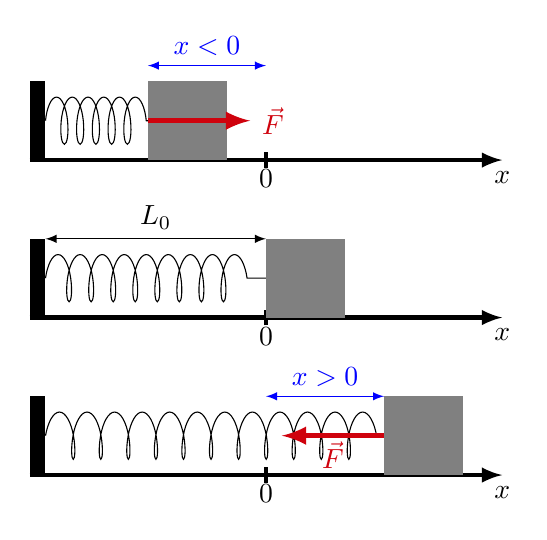
\begin{tikzpicture}[scale=1]
\tikzmath{
\L=2.;
\dx=0.75*\L;
\off=0.5;
\h=1;
}
\scalebox{1}{


\draw[-latex,line width=1.5pt] (-1.5*\L,0) -- (1.5*\L,0) node[below]{$x$};
\draw[line width=1.5pt] (0,-0.1) -- (0,0.1);
\node[below] at (0,0) {$0$};

\fill (-1.5*\L,0) rectangle (-1.4*\L,\h);
\draw[decoration={aspect=0.3, segment length=2.8mm, amplitude=3mm,coil},decorate] (-1.4*\L,\h/2) -- (0,\h/2);
\draw [latex-latex] (-1.4*\L,\h) -- (0,\h) node[midway,above]{$L_0$};
\fill[black!50] (0,0) rectangle (\h,\h);

%%%%%%%%%%  top compressed
\begin{scope}[shift={(0,2*\h)}]
\draw[-latex,line width=1.5pt] (-1.5*\L,0) -- (1.5*\L,0) node[below]{$x$};
\draw[line width=1.5pt] (0,-0.1) -- (0,0.1);
\node[below] at (0,0) {$0$};

\fill (-1.5*\L,0) rectangle (-1.4*\L,\h);
\draw[decoration={aspect=0.3, segment length=2mm, amplitude=3mm,coil},decorate] (-1.4*\L,\h/2) -- (-\dx,\h/2);
\draw [color=blue,latex-latex] (-\dx,1.2*\h) -- (0,1.2*\h) node[midway,above]{$x<0$};
\fill[black!50] (-\dx,0) rectangle (-\dx+\h,\h);
\draw[line width=2, -latex, color=myred] (-\dx,\h/2) -- +(1.3,0) node[right] {$\vec F$};

\end{scope}
%%%%%%%%%% bottom extended
\begin{scope}[shift={(0,-2*\h)}]
\draw[-latex,line width=1.5pt] (-1.5*\L,0) -- (1.5*\L,0) node[below]{$x$};
\draw[line width=1.5pt] (0,-0.1) -- (0,0.1);
\node[below] at (0,0) {$0$};

\fill (-1.5*\L,0) rectangle (-1.4*\L,\h);
\draw[decoration={aspect=0.3, segment length=3.5mm, amplitude=3mm,coil},decorate] (-1.4*\L,\h/2) -- (\dx,\h/2);
\draw [color=blue,latex-latex] (0,\h) -- (\dx,\h) node[midway,above]{$x>0$};
\fill[black!50] (\dx,0) rectangle (\dx+\h,\h);
\draw[line width=2, -latex, color=myred] (\dx,\h/2) -- +(-1.3,0) node[midway,below=-2pt] {$\vec F$};
\end{scope}

}
\end{tikzpicture}
\captionof*{figure}{\textit{A spring-mass system. When the moving end of the spring is at $x=0$, there is no spring force. When the moving end is in negative $x$ (compression), the force is in the positive direction. When the moving end is in positive $x$ (extension), the force is in the negative direction}.}
\end{center}


}


%%%%%%%%%%%%%%%%%%%%%%%%%%%%%%%%

\section{Free Body Diagrams}
\label{sec:fbds}
\title{Free Body Diagrams}
\institute{Newton's Laws}
\author{\insertsubsection}

%%%%%%%%%%%%


\begin{frame}
\titlepage
\thispagestyle{empty}
\end{frame}


%%%%%%%%%%%%%%%%%%%%%%%%%%%%%%%%
\subsection{Using Newton's second law}
\label{subsec:usingewtonssecondlaw}
\begin{frame}{Using Newton's second law}
\begin{enumerate}
\item Identify the forces (it's kinda important).
\item Make a \emph{good} FBD for each object with a mass:
\begin{enumerate}
\item Show the forces.
\item Show the acceleration vector.
\item Show your choice of coordinate system (a good choice is $\hat x$ parallel to $\vec a$ for that mass).
\item Show any relevant angles.
\end{enumerate}
\item Use the FBD to write out the components of Newton's Second Law for each mass.
\end{enumerate}

\end{frame}



%%%%%%%%%%%%%%%%%%%%%%%%%%%
\subsection{Hanging mass}
\label{subsec:hangingmass}
\begin{frame}{Group exercise: Draw FBD for each object}
 \begin{columns}[T]
 \column{0.5\textwidth}
\begin{center}
\begin{tikzpicture}[scale=1]
\tikzmath{
\L=1;
\myheight=0.631;
}
\scalebox{1.0}{
\node at (0,0) {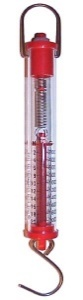
\includegraphics[scale=0.5]{figures/NewtonsLaws/scale}};
\fill [black!50] (-\L/2,-\L-\myheight) rectangle (\L/2,-\myheight);
\fill (-\L,\myheight) rectangle (\L,\myheight+0.2);
\node at (0,-\L/2-\myheight){$m$};

\fill (2*\L,\myheight+0.1) circle(3pt) node[right=2pt]{ceiling};
\fill (2.5*\L,0) circle(3pt) node[right=2pt]{scale};
\fill (2*\L,-\L/2-\myheight) circle(3pt) node[right=2pt]{mass};

}
\end{tikzpicture}
\end{center}
 \column{0.5\textwidth}
\begin{center}
\begin{tikzpicture}[scale=1]
\tikzmath{
\L=1;
\myheight=0.631;
}
\scalebox{1.0}{
\node at (0,\myheight) {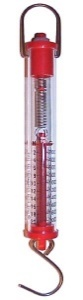
\includegraphics[scale=0.5]{figures/NewtonsLaws/scale}};
\node at (0,-\myheight) {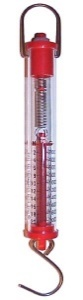
\includegraphics[scale=0.5]{figures/NewtonsLaws/scale}};
\fill (-\L,2*\myheight) rectangle (\L,2*\myheight+0.2);
\fill [black!50] (-\L/2,-\L-2*\myheight) rectangle (\L/2,-2*\myheight);
\node at (0,-\L/2-2*\myheight){$m$};

\fill (2*\L,2*\myheight+0.1) circle(3pt) node[right=2pt]{ceiling};
\fill (2.5*\L,\myheight) circle(3pt)node[right=2pt]{scale};
\fill (2*\L,-\myheight) circle(3pt)node[right=2pt]{scale};
\fill (2.5*\L,-\L/2-2*\myheight) circle(3pt)node[right=2pt]{mass};


}
\end{tikzpicture}
\end{center}
 \end{columns}
\begin{itemize}
\scriptsize
\item Assume the scales are massless.
\item Draw free body diagrams for the masses, scales and ceiling in both cases. (Draw little arrows around each point!).
\item Remember, all objects must have an acceleration of zero!
\item Be clear about what exerts a force on what!
\end{itemize}
\end{frame}


%%%%%%%%%%%%%%%%%%%%%%%%%%%%%%%%

\begin{frame}{Group exercise: Draw FBD for each object}
 \begin{columns}[T]
 \column{0.5\textwidth}
\begin{center}
\begin{tikzpicture}[scale=1]
\tikzmath{
\L=1;
\f=0.5;
\myheight=0.631;
}
\scalebox{1.0}{
\node at (0,0) {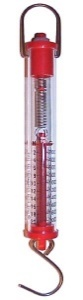
\includegraphics[scale=0.5]{figures/NewtonsLaws/scale}};
\fill [black!50] (-\L/2,-\L-\myheight) rectangle (\L/2,-\myheight);
\fill (-\L,\myheight) rectangle (\L,\myheight+0.2);
\node at (0,-\L/2-\myheight){$m$};

\fill (2*\L,\myheight+0.1) circle(3pt);
\draw [-latex,line width=1.5,color=myred] (2*\L,\myheight+0.1) -- +(0,\f) node[midway,right]{\scriptsize Force from building on ceiling};
\draw [-latex,line width=1.5] (2*\L,\myheight+0.1) -- +(0,-\f) node[midway,right]{\scriptsize Force from scale on ceiling};
\fill (2.5*\L,-0.25*\myheight) circle(3pt) ;
\draw [-latex,line width=1.5] (2.5*\L,-0.25*\myheight) -- +(0,\f) node[midway,right]{\scriptsize Force from ceiling on scale};
\draw [-latex,line width=1.5] (2.5*\L,-0.25*\myheight) -- +(0,-\f) node[midway,right]{\scriptsize Force from mass on scale};
\fill (2*\L,-\L/2-\myheight) circle(3pt) ;
\draw [-latex,line width=1.5] (2*\L,-\L/2-\myheight) -- +(0,\f) node[midway,right]{\scriptsize Force from scale on mass};
\draw [-latex,line width=1.5,color=myred] (2*\L,-\L/2-\myheight) -- +(0,-\f) node[midway,right]{\scriptsize Force from gravity on mass};
}
\end{tikzpicture}
\end{center}
 \column{0.5\textwidth}
\begin{center}
\begin{tikzpicture}[scale=1]
\tikzmath{
\L=1;
\f=0.5;
\myheight=0.631;
}
\scalebox{1.0}{
\node at (0,\myheight) {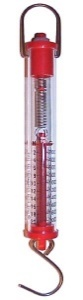
\includegraphics[scale=0.5]{figures/NewtonsLaws/scale}};
\node at (0,-\myheight) {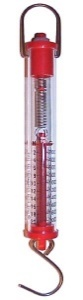
\includegraphics[scale=0.5]{figures/NewtonsLaws/scale}};
\fill (-\L,2*\myheight) rectangle (\L,2*\myheight+0.2);
\fill [black!50] (-\L/2,-\L-2*\myheight) rectangle (\L/2,-2*\myheight);
\node at (0,-\L/2-2*\myheight){$m$};

\fill (2*\L,2*\myheight+0.1) circle(3pt) ;
\draw [-latex,line width=1.5,color=myred] (2*\L,2*\myheight+0.1) -- +(0,\f) node[midway,right]{\scriptsize Force from building on ceiling};
\draw [-latex,line width=1.5] (2*\L,2*\myheight+0.1) -- +(0,-\f) node[midway,right]{\scriptsize Force from scale on ceiling};
\fill (2.5*\L,\myheight) circle(3pt);
\draw [-latex,line width=1.5] (2.5*\L,\myheight) -- +(0,\f) node[midway,right]{\scriptsize Force from ceiling on scale};
\draw [-latex,line width=1.5] (2.5*\L,\myheight) -- +(0,-\f) node[midway,right]{\scriptsize Force from scale on scale};
\fill (2*\L,-\myheight) circle(3pt);
\draw [-latex,line width=1.5] (2*\L,-\myheight)  -- +(0,\f) node[midway,right]{\scriptsize Force from scale on scale};
\draw [-latex,line width=1.5] (2*\L,-\myheight)  -- +(0,-\f) node[midway,right]{\scriptsize Force from mass on scale};
\fill (2.5*\L,-\L/2-2*\myheight) circle(3pt);
\draw [-latex,line width=1.5] (2.5*\L,-\L/2-2*\myheight) -- +(0,\f) node[midway,right]{\scriptsize Force from scale on mass};
\draw [-latex,line width=1.5,color=myred] (2.5*\L,-\L/2-2*\myheight) -- +(0,-\f) node[midway,right]{\scriptsize Force from gravity on mass};

}
\end{tikzpicture}
\end{center}
 \end{columns}
\begin{itemize}
\scriptsize
\item Two forces on each object, and they must have same magnitude/opposite direction.
\item The Earth and building (which holds up the ceiling) exert forces but are not shown. We only show bodies on which forces are exerted.
\item You need to become comfortable identifying forces that are exerted on objects!
\end{itemize}
\end{frame}

%%%%%%%%%%%%%%%%%%%%%%%%%%%%%%%%




%%%%%%%%%%%%%%%%%%%%%%%%%%%%%%%%
\subsection{Two masses, two pulleys and a spring scale}
\label{subsec:twomtwopspringscale}
\twocolframe{Group exercise: Draw the FBDs for masses and scale}
{

}
{

\begin{center}
\begin{tikzpicture}[scale=1]
\tikzmath{
\L=1.5;
\R=0.5;
\f=0.75;
\myheight=0.631;
}
\scalebox{1.0}{
\node at (0,0) {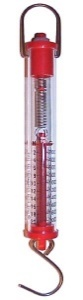
\includegraphics[scale=0.5,angle=90]{figures/NewtonsLaws/scale}};
\draw[line width=1.5] (\myheight,0) --+(\L,0);
\draw[line width=1.5] (-\myheight,0) --+(-\L,0);
\fill (0,\R) circle(3pt);

\fill[black!50] (-\L-\myheight,-\R) circle(\R);
\fill (-\L-\myheight,-\R) circle(3pt);
\draw[line width=1.5] (-\myheight-\L-\R,-\R) --+(0,-\L);
\fill[black!50] (-\myheight-\L-1.5*\R,-\R-\L) rectangle (-\myheight-\L-0.5*\R,-2*\R-\L);
\node at  (-\myheight-\L-\R,-1.5*\R-\L) {$m$};
\fill (-\myheight-\L-2.5*\R,-1.5*\R-\L) circle(3pt);

\fill[black!50] (\L+\myheight,-\R) circle(\R);
\fill (+\L+\myheight,-\R) circle(3pt);
\draw[line width=1.5] (\myheight+\L+\R,-\R) --+(0,-\L);
\fill[black!50] (\myheight+\L+1.5*\R,-\R-\L) rectangle (\myheight+\L+0.5*\R,-2*\R-\L);
\node at  (\myheight+\L+\R,-1.5*\R-\L) {$m$};
\fill (\myheight+\L+2.5*\R,-1.5*\R-\L) circle(3pt);

}
\end{tikzpicture}
\captionof*{figure}{\textit{Two masses, two pulleys and a spring scale.}}
\end{center}
}



%%%%%%%%%%%%%%%%%%%%%%%%%%%%%%%%
%%%%%%%%%%%%%%%%%%%%%%%%%%%%%%%%
\twocolframe{Group exercise: Draw the FBDs for masses and scale}
{
\begin{itemize}
\item All forces have the same magnitude, but the pulleys change the direction of tension forces in the ropes.
\item The forces exerted on the scale are the same as in the previous problem, so it reads the same!
\item The Earth exerts the two forces of gravity (in red).
\end{itemize}
}
{

\begin{center}
\begin{tikzpicture}[scale=1]
\tikzmath{
\L=1.5;
\R=0.5;
\f=0.75;
\myheight=0.631;
}
\scalebox{1.0}{
\node at (0,0) {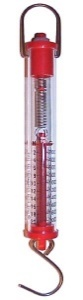
\includegraphics[scale=0.5,angle=90]{figures/NewtonsLaws/scale}};
\draw[line width=1.5] (\myheight,0) --+(\L,0);
\draw[line width=1.5] (-\myheight,0) --+(-\L,0);
\fill (0,\R) circle(3pt) node[above]{\scriptsize Forces exerted by ropes on scale};
\draw [-latex,line width=1.5] (0,\R)  -- +(\f,0) ; 
\draw [-latex,line width=1.5] (0,\R)  -- +(-\f,0); 

\fill[black!50] (-\L-\myheight,-\R) circle(\R);
\fill (-\L-\myheight,-\R) circle(3pt);
\draw[line width=1.5] (-\myheight-\L-\R,-\R) --+(0,-\L);
\fill[black!50] (-\myheight-\L-1.5*\R,-\R-\L) rectangle (-\myheight-\L-0.5*\R,-2*\R-\L);
\node at  (-\myheight-\L-\R,-1.5*\R-\L) {$m$};
\fill (-\myheight-\L-2.5*\R,-1.5*\R-\L) circle(3pt);
\draw [-latex,line width=1.5] (-\myheight-\L-2.5*\R,-1.5*\R-\L)   -- +(0,\f) ; 
\draw [-latex,line width=1.5,color=myred] (-\myheight-\L-2.5*\R,-1.5*\R-\L)   -- +(0,-\f); 


\fill[black!50] (\L+\myheight,-\R) circle(\R);
\fill (+\L+\myheight,-\R) circle(3pt);
\draw[line width=1.5] (\myheight+\L+\R,-\R) --+(0,-\L);
\fill[black!50] (\myheight+\L+1.5*\R,-\R-\L) rectangle (\myheight+\L+0.5*\R,-2*\R-\L);
\node at  (\myheight+\L+\R,-1.5*\R-\L) {$m$};
\fill (\myheight+\L+2.5*\R,-1.5*\R-\L) circle(3pt);
\draw [-latex,line width=1.5] (\myheight+\L+2.5*\R,-1.5*\R-\L)   -- +(0,\f); 
\draw [-latex,line width=1.5,color=myred] (\myheight+\L+2.5*\R,-1.5*\R-\L)   -- +(0,-\f); 

}
\end{tikzpicture}
\captionof*{figure}{\textit{Two masses, two pulleys and a spring scale}}
\end{center}
}
%%%%%%%%%%%%%%%%%%%%%%%%%%%
\subsection{Two blocks on an inclined plane}
\label{subsec:twoblocksonaninclinedplane}
\begin{frame}{Draw the FBD for each block}
\begin{center}
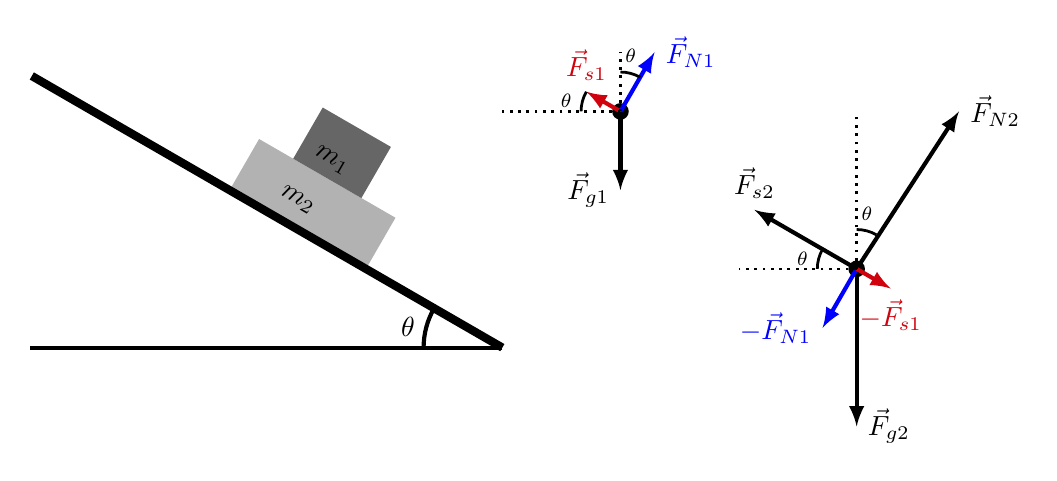
\begin{tikzpicture}[scale=1]
\tikzmath{
\L=6;
\R=0.125*\L/2;
\th=30;
\h=\L*sin(\th);
\hR=0.125*\L;
\vgg=1.;
\fsll=\vgg*sin(\th);
\Nxx=\fsll*cos(\th);
\Nyy=\vgg-\fsll*sin(\th);
\vg=2*\vgg;
\fsl=\vg*sin(\th)+\fsll;
\Nx=\fsl*cos(\th);
\Ny=\Nyy+\vg-\fsl*sin(\th);
}
\scalebox{1.0}{

\coordinate (P2) at (0.75*\L,\h/3);
\coordinate (P1) at (\L/4,\h);

%Blockw
\fill[black!30, rotate=-\th, shift={(-\L/2,0)}] (-\L/6,0) rectangle (\L/6,\L/8);
\node[rotate=-\th, shift={(-\L/2,0)}] at (0,\L/16){$m_2$};
\fill[black!60, rotate=-\th, shift={(-\L/2,0)}] (-\L/12,\L/8) rectangle (\L/12,\L/4);
\node[rotate=-\th, shift={(-\L/2+\L/12,0)}] at (0,\hR+\R){$m_1$};
%\fill[black, rotate=-\th, shift={(-\L,0)}] (-0.1,0) rectangle (0.,\L/3);

\draw[line width=3pt,rotate=-\th] (0,0) -- (-1.15*\L,0);
\draw[line width=1.5pt] (0,0) -- (-\L,0);
\draw[line width=1.5pt] (-1,0) arc (180:180-\th:1) node[midway,left]{$\theta$};

\fill (P1) circle(3pt);
\fill (P2) circle(3pt);

\only<2>{

\draw[-latex,line width=1.5pt] (P2) -- +(0,-\vg) node[right]{$\vec F_{g2}$};
\draw[-latex,line width=1.5pt] (P1) -- +(0,-\vgg) node[left]{$\vec F_{g1}$};

\draw[-latex,line width=1.5pt] (P2) -- +(\Nx,\Ny) node[right]{$\vec F_{N2}$};
\draw[-latex,line width=1.5pt,color=blue] (P1) -- +(\Nxx,\Nyy) node[right]{$\vec F_{N1}$};
\draw[-latex,line width=1.5pt,color=blue] (P2) -- +(-\Nxx,-\Nyy) node[left]{$-\vec F_{N1}$};


\draw[-latex,line width=1.5pt] (P2) -- +(180-\th:\fsl) node[above]{$\vec F_{s2}$};
\draw[-latex,line width=1.5pt,color=myred] (P1) -- +(180-\th:\fsll) node[above]{$\vec F_{s1}$};
\draw[-latex,line width=1.5pt,color=myred] (P2) -- +(-\th:\fsll) node[below]{$-\vec F_{s1}$};

\draw[dotted, line width=1] (P2) -- +(-\fsl,0);
\draw[dotted, line width=1] (P1) -- +(-\fsl,0);

\draw[dotted, line width=1] (P2) -- +(0,\Ny);
\draw[dotted, line width=1] (P1) -- +(0,\Nyy);

\draw[line width=1] ($(P2)+(0,0.5)$) arc(90:90-\th:0.5)node[midway,above]{\scriptsize$\theta$};
\draw[line width=1] ($(P2)+(-0.5,0)$) arc(180:180-\th:0.5)node[midway,left]{\scriptsize$\theta$};
\draw[line width=1] ($(P1)+(0,0.5)$) arc(90:90-\th:0.5)node[midway,above]{\scriptsize$\theta$};
\draw[line width=1] ($(P1)+(-0.5,0)$) arc(180:180-\th:0.5)node[midway,left]{\scriptsize$\theta$};
}

}
\end{tikzpicture}
\only<1>{
\captionof*{figure}{\textit{Two blocks on an inclined plane.}}}
\only<2>{
\captionof*{figure}{\textit{Two blocks on an inclined plane, with free body diagram. Arrows of the same colour represent action and reaction ``pairs'', which are \emph{necessarily} exerted on different bodies (Newton's Third Law).}}}
\end{center}
\end{frame}


%%%%%%%%%%%%%%%%%%%%%%%%%%%%%%%
\subsection{Two blocks on an inclined plane + pulley}
\label{subsec:twoblocksonaninclinedplanepluspulley}
\begin{frame}{Draw the FBD for each block}
\begin{center}
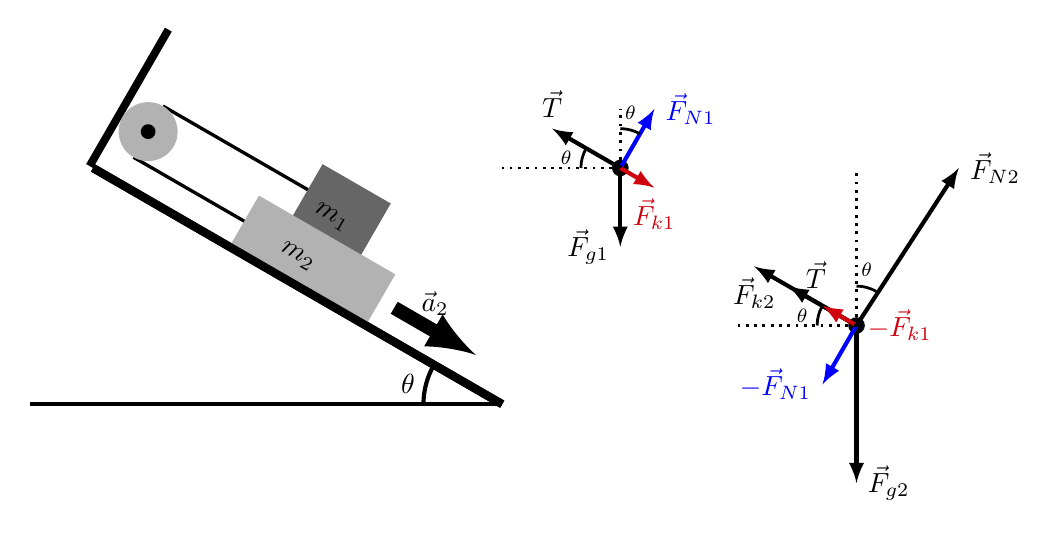
\begin{tikzpicture}[scale=1]
\tikzmath{
\L=6;
\R=0.125*\L/2;
\th=30;
\h=\L*sin(\th);
\hR=0.125*\L;
\vgg=1.;
\fsll=\vgg*sin(\th);
\Nxx=\fsll*cos(\th);
\Nyy=\vgg-\fsll*sin(\th);
\vg=2*\vgg;
\fsl=\vg*sin(\th)+\fsll;
\Nx=\fsl*cos(\th);
\Ny=\Nyy+\vg-\fsl*sin(\th);
}
\pgfmathsetmacro{\T}{1}
\scalebox{1.0}{

\coordinate (P2) at (0.75*\L,\h/3);
\coordinate (P1) at (\L/4,\h);

\draw[line width=3pt,rotate=-\th] (0,0) -- (-\L,0);% -- (-\L, \h) -- cycle;

\fill[black!30, rotate=-\th, shift={(-\L/2,0)}] (-\L/6,0) rectangle (\L/6,\L/8);
\node[rotate=-\th, shift={(-\L/2,0)}] at (0,\L/16){$m_2$};
\fill[black!60, rotate=-\th, shift={(-\L/2,0)}] (-\L/12,\L/8) rectangle (\L/12,\L/4);
\node[rotate=-\th, shift={(-\L/2+\L/12,0)}] at (0,\hR+\R){$m_1$};
\fill[black, rotate=-\th, shift={(-\L,0)}] (-0.1,0) rectangle (0.,\L/3);

%ropes:
\draw[line width = 1.2pt,rotate=-\th, shift={(-\L/2,0)}](-\L/2+\R,\hR-\R) -- (-\L/6,\L/16) ;
\draw[line width = 1.2pt,rotate=-\th, shift={(-\L/2,0)}](-\L/2+\R,\hR+\R) -- (-\L/12, 0.1875*\L) ;
%pulley
\fill[black!30, rotate=-\th, shift={(-\L+\R,0)}] (0,\hR) circle(\R);
\fill[black, rotate=-\th, shift={(-\L+\R,0)}] (0,\hR) circle(0.25*\R);

%plane
\draw[line width=3pt,rotate=-\th] (0,0) -- (-\L,0);
\draw[line width=1.5pt] (0,0) -- (-\L,0);
\draw[line width=1.5pt] (-1,0) arc (180:180-\th:1) node[midway,left]{$\theta$};

%acceleration arrow
\draw [line width = 5pt, -latex,rotate=-\th, shift={(-\L/2,0)}] (0.2*\L, \L/16)--+(\L/5,0) node[midway,above] {$\vec a_2$};

\fill (P1) circle(3pt);
\fill (P2) circle(3pt);

\only<2>{

\draw[-latex,line width=1.5pt] (P2) -- +(0,-\vg) node[right]{$\vec F_{g2}$};
\draw[-latex,line width=1.5pt] (P1) -- +(0,-\vgg) node[left]{$\vec F_{g1}$};

\draw[-latex,line width=1.5pt] (P2) -- +(\Nx,\Ny) node[right]{$\vec F_{N2}$};
\draw[-latex,line width=1.5pt,color=blue] (P1) -- +(\Nxx,\Nyy) node[right]{$\vec F_{N1}$};
\draw[-latex,line width=1.5pt,color=blue] (P2) -- +(-\Nxx,-\Nyy) node[left]{$-\vec F_{N1}$};

\draw[-latex,line width=1.5pt] (P2) -- +(180-\th:\T) node[right=10pt,above=-5pt]{$\vec T$};
\draw[-latex,line width=1.5pt] (P1) -- +(180-\th:\T) node[above]{$\vec T$};

\draw[-latex,line width=1.5pt] (P2) -- +(180-\th:\fsl) node[below]{$\vec F_{k2}$};
\draw[-latex,line width=1.5pt,color=myred] (P2) node[right ]{$-\vec F_{k1}$}-- +(180-\th:\fsll) ;
\draw[-latex,line width=1.5pt,color=myred] (P1) -- +(-\th:\fsll) node[below]{$\vec F_{k1}$};

\draw[dotted, line width=1] (P2) -- +(-\fsl,0);
\draw[dotted, line width=1] (P1) -- +(-\fsl,0);

\draw[dotted, line width=1] (P2) -- +(0,\Ny);
\draw[dotted, line width=1] (P1) -- +(0,\Nyy);

\draw[line width=1] ($(P2)+(0,0.5)$) arc(90:90-\th:0.5)node[midway,above]{\scriptsize$\theta$};
\draw[line width=1] ($(P2)+(-0.5,0)$) arc(180:180-\th:0.5)node[midway,left]{\scriptsize$\theta$};
\draw[line width=1] ($(P1)+(0,0.5)$) arc(90:90-\th:0.5)node[midway,above]{\scriptsize$\theta$};
\draw[line width=1] ($(P1)+(-0.5,0)$) arc(180:180-\th:0.5)node[midway,left]{\scriptsize$\theta$};
}

}
\end{tikzpicture}
\only<1>{
\captionof*{figure}{\textit{Two blocks on an inclined plane with pulley.}}}
\only<2>{
\captionof*{figure}{\textit{Two blocks on an inclined plane with pulley, with free body diagram. Arrows of the same colour represent action and reaction ``pairs'', which are \emph{necessarily} exerted on different bodies (Newton's Third Law).}}}
\end{center}
\end{frame}


%%%%%%%%%%%%%%%%%%%%%%%%%%%%%%%%



%%%%%%%%%%%%%%%%%%%%%%%%%%%%%%%%
\subsection {Applying Newton's 2nd law using a FBD}
\label{subsec:applyingnewtonssecondlawtoblock1}
\twocolframe{Applying Newton's Second Law to block 1}
{
We ``simply'' read off the FBD to obtain the two components of Newton's Second Law:
\begin{align*}
\sum F_x \rightarrow &T-F_{k1}-F_{g1}\sin\theta&=&m_1a_1\\
\sum F_y \rightarrow &F_{N1}-F_{g1}\cos\theta&=&0
\end{align*}
You would do the same for block 2, noting that $a_1=a_2$, since the \emph{magnitude} of the acceleration of the two blocks must be the same (they are connected by a rope).
}
{
\begin{center}
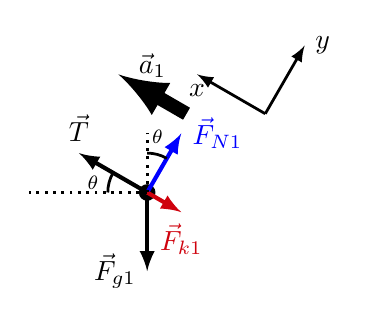
\begin{tikzpicture}[scale=1]
\tikzmath{
\L=6;
\R=0.125*\L/2;
\th=30;
\h=\L*sin(\th);
\hR=0.125*\L;
\vgg=1.;
\fsll=\vgg*sin(\th);
\Nxx=\fsll*cos(\th);
\Nyy=\vgg-\fsll*sin(\th);
\vg=2*\vgg;
\fsl=\vg*sin(\th)+\fsll;
\Nx=\fsl*cos(\th);
\Ny=\Nyy+\vg-\fsl*sin(\th);
}
\pgfmathsetmacro{\T}{1}
\scalebox{1.0}{

\coordinate (P1) at (\L/4,\h);

\fill (P1) circle(3pt);

%coordinates
\draw[-latex,line width=1pt] ($(P1)+(1.5,1.)$) -- +(180-\th:1) node[below]{$x$};
\draw[-latex,line width=1pt] ($(P1)+(1.5,1.)$) -- +(90-\th:1) node[right]{$y$};
\draw[-latex,line width=5pt] ($(P1)+(0.5,1)$) -- +(180-\th:1) node[midway,above]{$\vec a_1$};

\draw[-latex,line width=1.5pt] (P1) -- +(0,-\vgg) node[left]{$\vec F_{g1}$};

\draw[-latex,line width=1.5pt,color=blue] (P1) -- +(\Nxx,\Nyy) node[right]{$\vec F_{N1}$};

\draw[-latex,line width=1.5pt] (P1) -- +(180-\th:\T) node[above]{$\vec T$};


\draw[-latex,line width=1.5pt,color=myred] (P1) -- +(-\th:\fsll) node[below]{$\vec F_{k1}$};


\draw[dotted, line width=1] (P1) -- +(-\fsl,0);

\draw[dotted, line width=1] (P1) -- +(0,\Nyy);

\draw[line width=1] ($(P1)+(0,0.5)$) arc(90:90-\th:0.5)node[midway,above]{\scriptsize$\theta$};
\draw[line width=1] ($(P1)+(-0.5,0)$) arc(180:180-\th:0.5)node[midway,left]{\scriptsize$\theta$};


}
\end{tikzpicture}
\captionof*{figure}{\textit{Free-body diagram for $m_1$ from the previous slide.}}
\end{center}
}

%%%%%%%%%%%%%%%%%%%%%%%%%%%%%%%%

%%%%%%%%%%%%%%%%%%%%%%%%%%%%%%%%
\subsection{Blocs on an incline connected via pulley}
\label{subsec:blocksonaninclineconnectedbyapulley}
\twocolframe{Blocks on an incline}
{
\begin{center}
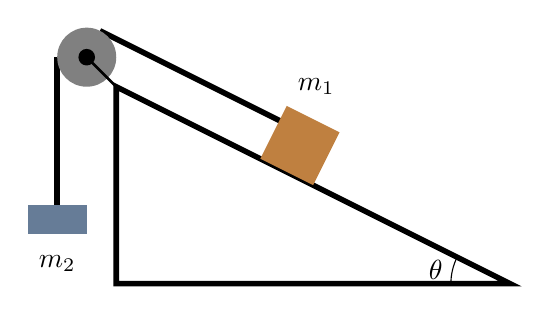
\begin{tikzpicture}[scale=1]
\tikzmath{
\L=5;
\h=2.5;
\abox=0.75;
\R=0.5*\abox;
\th=atan(\h/\L);
\d=\R+\L*cos(\th)/2;
}
\scalebox{1.0}{
\coordinate (Pb1) at (\L/2,\h/2);%coordinates of box
\coordinate (Pb2) at ($(Pb1)+(180-\th:\abox)$);
\coordinate (Pb3) at ($(Pb2)+(90-\th:\abox)$);
\coordinate (Pb4) at ($(Pb3)+(-\th:\abox)$);
\coordinate (Pc) at (-\R,\h+\R);


%plane and angle
\draw[line width=2pt] (0,\h) -- (0,0) -- (\L,0) -- cycle;
\draw (\L-0.75,0) arc(180:180-\th:0.75) node[midway,left]{$\theta$};


%ropes
\draw[line width=2] ($(Pc)+(90-\th:\R)$) -- +(-\th:\d);
\draw[line width=2] (-2*\R,\h+\R) -- +(0,-0.75*\h);

%pulley

\fill[color=black!50] (Pc) circle (\R);
\fill (Pc) circle(3pt);
\draw[line width=1] (Pc) -- (0,\h);

%rotated boxes
\fill[color=brown] (Pb1) -- (Pb2) -- (Pb3) -- (Pb4) -- cycle ;
\fill[color=myblue!60, shift={(-3*\R,0.25*\h)}] (0,0) rectangle (\abox,0.5*\abox);

\node at ($(Pb3)+(\abox/2,\abox/3)$) {$m_1$};
\node at (-2*\R,0.1*\h) {$m_2$};
}
\end{tikzpicture}
\captionof*{figure}{\textit{Two blocks connected by a pulley.}}
\end{center}
}
{
Draw the free body diagrams for both block when they accelerate.
}

%%%%%%%%%%%%%%%%%%%%%%%%%%%%%%%%

\twocolframe{Blocks on an incline}
{
\begin{center}
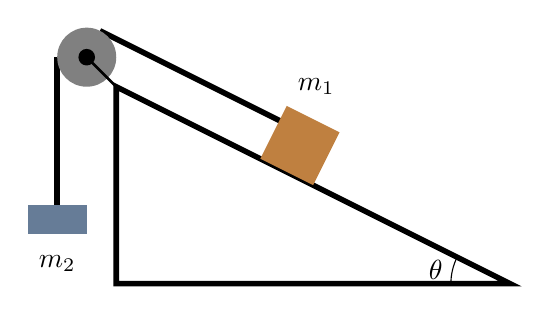
\begin{tikzpicture}[scale=1]
\tikzmath{
\L=5;
\h=2.5;
\abox=0.75;
\R=0.5*\abox;
\th=atan(\h/\L);
\d=\R+\L*cos(\th)/2;
}
\scalebox{1.0}{
\coordinate (Pb1) at (\L/2,\h/2);%coordinates of box
\coordinate (Pb2) at ($(Pb1)+(180-\th:\abox)$);
\coordinate (Pb3) at ($(Pb2)+(90-\th:\abox)$);
\coordinate (Pb4) at ($(Pb3)+(-\th:\abox)$);
\coordinate (Pc) at (-\R,\h+\R);


%plane and angle
\draw[line width=2pt] (0,\h) -- (0,0) -- (\L,0) -- cycle;
\draw (\L-0.75,0) arc(180:180-\th:0.75) node[midway,left]{$\theta$};


%ropes
\draw[line width=2] ($(Pc)+(90-\th:\R)$) -- +(-\th:\d);
\draw[line width=2] (-2*\R,\h+\R) -- +(0,-0.75*\h);

%pulley

\fill[color=black!50] (Pc) circle (\R);
\fill (Pc) circle(3pt);
\draw[line width=1] (Pc) -- (0,\h);

%rotated boxes
\fill[color=brown] (Pb1) -- (Pb2) -- (Pb3) -- (Pb4) -- cycle ;
\fill[color=myblue!60, shift={(-3*\R,0.25*\h)}] (0,0) rectangle (\abox,0.5*\abox);

\node at ($(Pb3)+(\abox/2,\abox/3)$) {$m_1$};
\node at (-2*\R,0.1*\h) {$m_2$};
}
\end{tikzpicture}
\captionof*{figure}{\textit{Two blocks connected by a pulley.}}
\end{center}
}
{
\begin{center}
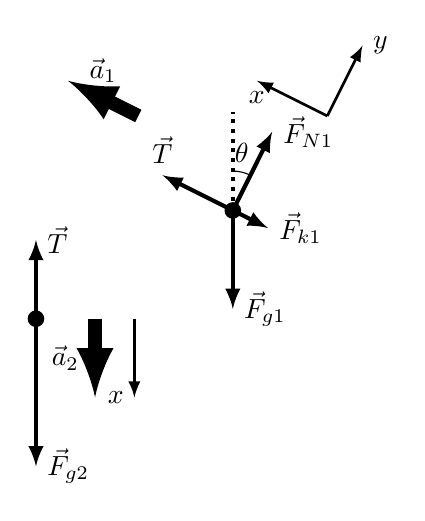
\begin{tikzpicture}[scale=1]
\tikzmath{
\L=5;
\h=2.5;
\th=atan(\h/\L);
\vg=1.25;
\fk=0.5;
\No=\vg*cos(\th);
\vgg=1.5*\vg;
}
\pgfmathsetmacro{\T}{1}
\scalebox{1.0}{

\coordinate (P1) at (0,0.75*\h);
\coordinate (P2) at (-\h,0.2*\h);

\fill (P1) circle (3pt);
\fill (P2) circle (3pt);

%for mass 1
\draw[-latex,line width=1.5pt] (P1) -- +(0,-\vg) node[right] {$\vec F_{g1}$};
\draw[-latex,line width=1.5pt] (P1) -- +(180-\th:\T) node[above] {$\vec T$};
\draw[-latex,line width=1.5pt] (P1) -- +(-\th:\fk) node[right] {$\vec F_{k1}$};
\draw[-latex,line width=1.5pt] (P1) -- +(90-\th:\No) node[right] {$\vec F_{N1}$};
\draw[dotted,line width=1.5pt] (P1) -- +(0,\vg);
\draw ($(P1)+(0,0.5)$) arc (90:90-\th:0.5) node[midway,above] {$\theta$};

\draw[-latex,line width=1.pt] ($(P1)+(1.2,1.2)$) -- +(180-\th:1) node[below]{$x$};
\draw[-latex,line width=1.pt] ($(P1)+(1.2,1.2)$) -- +(90-\th:1) node[right]{$y$};
\draw[-latex,line width=5pt] ($(P1)+(-1.2,1.2)$) -- +(180-\th:1) node[midway,above]{$\vec a_1$};


%for mass 2
\draw[-latex,line width=1.5pt] (P2) -- +(0,-\vgg) node[right] {$\vec F_{g2}$};
\draw[-latex,line width=1.5pt] (P2) -- +(0,\T) node[right] {$\vec T$};
\draw[-latex,line width=5pt] ($(P2)+(0.75,0)$) -- +(0,-1) node[midway, left]{$\vec a_2$};
\draw[-latex,line width=1.pt] ($(P2)+(1.25,0)$) -- +(0,-1) node[left]{$x$};
}
\end{tikzpicture}
\captionof*{figure}{\textit{Free body diagrams for the two blocks.}}
\end{center}
}




























%%%%%%%%%%%%%%%%%%%%%%%%%%%%%%%%

\title{Applying Newton's Laws}
\subject{Motion, Derivations and Modelling Situations}
\subtitle{Building Models to Describe our World}


%%%%%%%%%%%%%%%%%%%%%%%%%
%%%%%% Title slide %%%%%%
%%%%%%%%%%%%%%%%%%%%%%%%%
\chaptertitle{Applying Newton's Laws}
\begin{frame}
\label{chap:applyingnewtonslaws}
\titlepage
\thispagestyle{empty}

\begin{textblock*}{5cm}(11cm,4cm)
    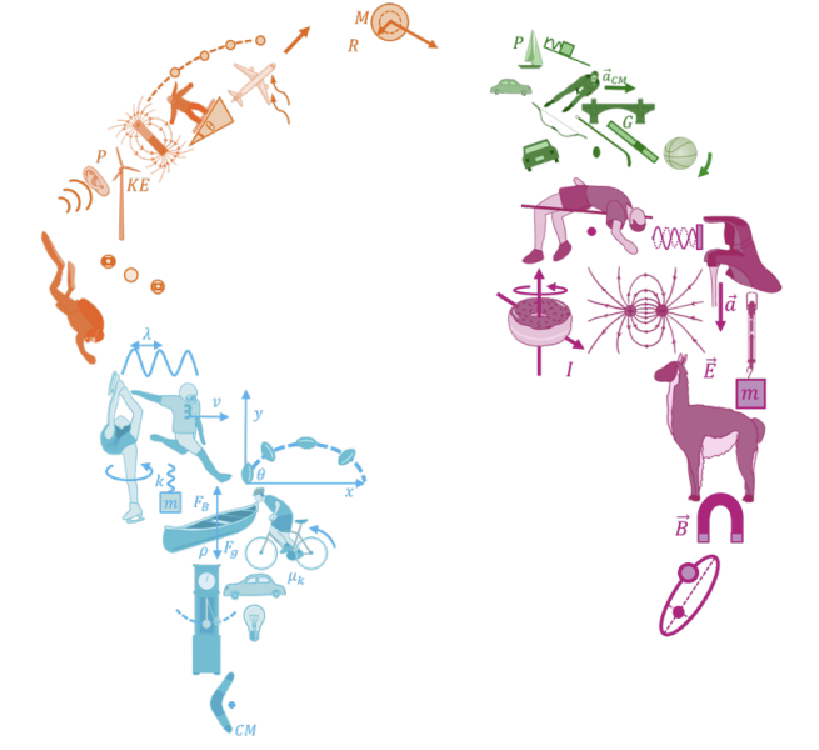
\includegraphics[width=4cm]{figures/BMDW/logo}
\end{textblock*}

\end{frame}
%%%%%%%%%%%%%%%%%%%%%%%%


\twocolframe{Outline}
{\tableofcontents[sections=13, subsectionstyle=show/show]\thispagestyle{empty}}
{\tableofcontents[sections=14-15, subsectionstyle=show/show]}







%%%%%%%%%%%%%%%%%%%%%%%%%%%%%%%%
\section{Types of Motion}
\label{sec:typesofmotion}
\title{Types of Motion}


%%%%%%%%%%%%%%%%%%%%%%%%%
\begin{frame}
\titlepage
\thispagestyle{empty}
\end{frame}



%%%%%%%%%%%%%%%%%%%%%%%
\subsection{Linear motion}
\label{subsec:linearmotion}
\begin{frame}{Linear motion}
\begin{itemize}
\item We can loosely define ``linear motion'' as motion along a straight line, where the velocity does not change direction.
\item The net force (and acceleration) is co-linear with the velocity.
\item We can break up many types of motion into segments where the motion is linear along the segments.
\end{itemize}

\begin{center}
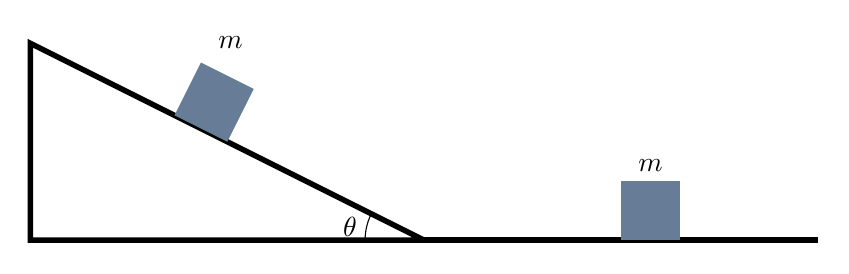
\begin{tikzpicture}[scale=1]
\tikzmath{
\L=5;
\h=2.5;
\abox=0.75;
\R=0.5*\abox;
\th=atan(\h/\L);
\d=\R+\L*cos(\th)/2;
}
\scalebox{1.0}{
\coordinate (Pb1) at (\L/2,\h/2);%coordinates of box
\coordinate (Pb2) at ($(Pb1)+(180-\th:\abox)$);
\coordinate (Pb3) at ($(Pb2)+(90-\th:\abox)$);
\coordinate (Pb4) at ($(Pb3)+(-\th:\abox)$);

%plane and angle
\draw[line width=2pt] (0,\h) -- (0,0) -- (\L,0) -- cycle;
\draw[line width=2pt] (\L,0) -- (2*\L,0);
\draw (\L-0.75,0) arc(180:180-\th:0.75) node[midway,left]{$\theta$};


%boxes
\fill[color=myblue!60] (Pb1) -- (Pb2) -- (Pb3) -- (Pb4) -- cycle ;
\fill[color=myblue!60] (1.5*\L,0) rectangle (1.5*\L+\abox,\abox);

\node at ($(Pb3)+(\abox/2,\abox/3)$) {$m$};
\node[above] at (1.5*\L+0.5*\abox,\abox) {$m$};
}
\end{tikzpicture}
\captionof*{figure}{\textit{A block slides down an incline and then a flat section. Both segments are linear motion.}}
\end{center}

\end{frame}


%%%%%%%%%%%%%%%%%%%%%%%%%%%%%%%%
\subsection{Constant net force}
\label{subsec:cnstnetforce}
\begin{frame}{Constant net force}
\begin{itemize}
\item When the \textbf{sum of the forces} (aka the net force) on an object is constant (in magnitude and direction), and the mass of the object is constant, the acceleration of that object is constant:
\begin{align*}
\sum \vec F = \vec F^{net}=m\vec a
\end{align*}
\item When the acceleration is constant:
\begin{align*}
\vec v(t) &= \vec v_0+\vec at=\vec v_0+\frac{\vec F^{net}}{m}t\\
\vec r(t) &= \vec r_0+\vec v_0 t+\frac{1}{2}\vec a t^2=\vec r_0+\vec v_0 t+\frac{1}{2} \frac{\vec F^{net}}{m} t^2
\end{align*}
\item This is a vector equation, so true by component, for example, the $x$ component:
\begin{align*}
v_x(t)=v_{0x}+\frac{F_x}{m}t\quad x(t)=x_0+v_{0x}t+\frac{1}{2}\frac{F_x}{m}t^2
\end{align*}
\end{itemize}

\end{frame}


%%%%%%%%%%%%%%%%%%%%%%%%%%%%%%%%
\subsection{Varying net force}
\label{subsec:varying net force}
\begin{frame}{Varying net force}
\begin{itemize}
\item The net force on an object can change magnitude and direction:
\begin{itemize}
\item As a function of time.
\item As a function of position.
\item As a function of velocity.
\end{itemize}
\item Then, the acceleration is not constant, and we have to start with:
\begin{align*}
\frac{d\vec v}{dt}&=\vec a = \frac{\vec F^{net}}{m}\\
\frac{d\vec r}{dt}&=\vec v
\end{align*}
and integrate...
\end{itemize}

\end{frame}


%%%%%%%%%%%%%%%%%%%%%%%%%%%%%%%%
\subsubsection{Varying with time}
\label{subsubsec:varyingwithtime}
\begin{frame}{Linear motion, force varies with time}
\begin{itemize}
\item If the magnitude of the force changes with time:
\begin{align*}
\vec a(t)=\frac{\vec F^{net}(t)}{m}
\end{align*}
\item The kinematics equations are ``straightforward'':
\begin{align*}
\frac{d\vec v}{dt}&=\frac{1}{m}\vec F^{net}(t)\\
\therefore \vec v(t)&=\vec v_0+\frac{1}{m}\int_0^t \vec F^{net}(t) dt\\
\therefore \vec r(t)&=\vec r_0+\int_0^t \vec v(t) dt\\
\end{align*}
just some integrals that you can look up if you know the function $\vec F^{net}(t)$...
\end{itemize}

\end{frame}


%%%%%%%%%%%%%%%%%%%%%%%%%%%%%%%%


%%%%%%%%%%%%%%%%%%%%%%%%%%%%%%%%
\subsubsection{Varying with position}
\label{subsubsec:varyingwithposition}
\begin{frame}{Linear motion, force varies with position}
\begin{itemize}
\item If the magnitude of the force changes with position of the object:
\begin{align*}
 a_x(x)=\frac{F^{net}_x(x)}{m}
\end{align*}
\item We cannot ``simply integrate'' the equations that define acceleration from velocity and velocity from position:
\begin{align*}
\frac{dv_x}{dt}=a_x(x) \rightarrow v_x(t)=v_{0x}+\int_0^ta_x(x)dt
\end{align*}
\end{itemize}

\only<2>{
\begin{tikzpicture}[remember picture,overlay]
\coordinate (X1) at ($(current page.center)+(-0.5,0.35)$);
\coordinate (X2) at ($(X1)+(0,-1)$);
\coordinate (X3) at ($(X1)+(4.5,0)$);
\coordinate (X4) at ($(X3)+(0,-1)$);

\draw[color=myred,line width=5] (X1) -- (X4);
\draw[color=myred,line width=5] (X3) -- (X2);

\end{tikzpicture}
}

\begin{center}
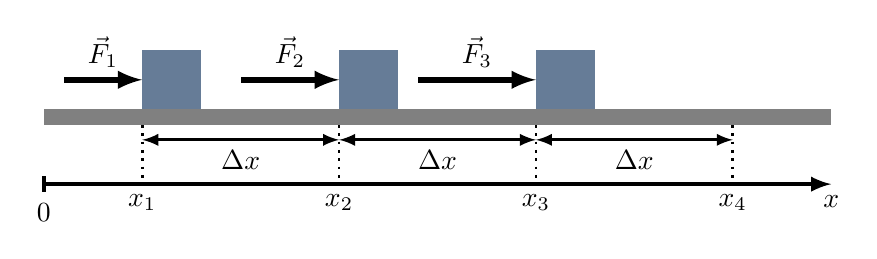
\begin{tikzpicture}[scale=1]
\tikzmath{
\L=10;
\h=0.75;
\w=0.2;
\dx=2.5;
\abox=0.75;
\Fm=1;
}
\scalebox{1.0}{
%axis
\draw[-latex, line width=1.5pt] (0,0) -- (\L,0) node[below]{$x$};
\draw[line width=1.5pt] (0,0.1) -- (0,-0.1) node[below]{$0$};
%floor
\fill[black!50] (0,\h) rectangle (\L,\h+\w);

\fill[color=myblue!60] (0.5*\dx,\h+\w) rectangle (0.5*\dx+\abox,\h+\w+\abox);
\fill[color=myblue!60] (1.5*\dx,\h+\w) rectangle (1.5*\dx+\abox,\h+\w+\abox);
\fill[color=myblue!60] (2.5*\dx,\h+\w) rectangle (2.5*\dx+\abox,\h+\w+\abox);

\draw[latex-,line width=2] (0.5*\dx,\h+\w+\abox/2) -- +(-\Fm,0) node[midway,above]{$\vec F_1$};
\draw[latex-,line width=2] (1.5*\dx,\h+\w+\abox/2) -- +(-1.25*\Fm,0) node[midway,above]{$\vec F_2$};
\draw[latex-,line width=2] (2.5*\dx,\h+\w+\abox/2) -- +(-1.5*\Fm,0) node[midway,above]{$\vec F_3$};

\draw[dotted, line width=1] (0.5*\dx,\h) -- +(0,-\h) node[below]{$x_1$};
\draw[dotted, line width=1] (1.5*\dx,\h) -- +(0,-\h) node[below]{$x_2$};
\draw[dotted, line width=1] (2.5*\dx,\h) -- +(0,-\h) node[below]{$x_3$};
\draw[dotted, line width=1] (3.5*\dx,\h) -- +(0,-\h) node[below]{$x_4$};

\draw[latex-latex, line width=1] (0.5*\dx,0.75*\h)--+(\dx,0) node[midway, below]{$\Delta x$};
\draw[latex-latex, line width=1] (1.5*\dx,0.75*\h)--+(\dx,0) node[midway, below]{$\Delta x$};
\draw[latex-latex, line width=1] (2.5*\dx,0.75*\h)--+(\dx,0) node[midway, below]{$\Delta x$};
}
\end{tikzpicture}
\captionof*{figure}{\textit{A block slides along $x$ with a force that changes depending on position.}}
\end{center}
\end{frame}



%%%%%%%%%%%%%%%%%%%%%%%%%%%%%%%%
\subsection{Breaking up motion}
\label{subsec:breakingupmotion}
\begin{frame}{Breaking it up}
\begin{itemize}
\item When things vary continuously, we can break up the motion into small segments where things are constant (in this case, things = force, acceleration).
\end{itemize}

\begin{center}
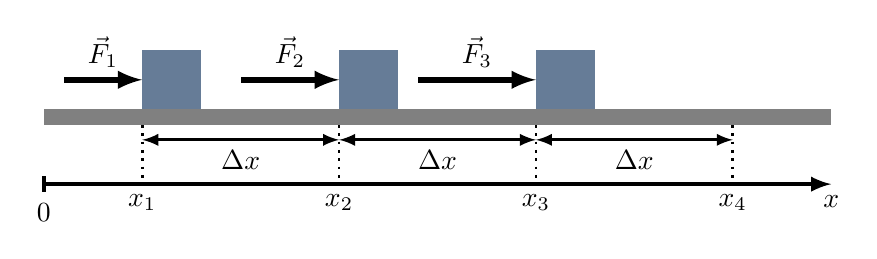
\begin{tikzpicture}[scale=1]
\tikzmath{
\L=10;
\h=0.75;
\w=0.2;
\dx=2.5;
\abox=0.75;
\Fm=1;
}
\scalebox{1.0}{
%axis
\draw[-latex, line width=1.5pt] (0,0) -- (\L,0) node[below]{$x$};
\draw[line width=1.5pt] (0,0.1) -- (0,-0.1) node[below]{$0$};
%floor
\fill[black!50] (0,\h) rectangle (\L,\h+\w);

\fill[color=myblue!60] (0.5*\dx,\h+\w) rectangle (0.5*\dx+\abox,\h+\w+\abox);
\fill[color=myblue!60] (1.5*\dx,\h+\w) rectangle (1.5*\dx+\abox,\h+\w+\abox);
\fill[color=myblue!60] (2.5*\dx,\h+\w) rectangle (2.5*\dx+\abox,\h+\w+\abox);

\draw[latex-,line width=2] (0.5*\dx,\h+\w+\abox/2) -- +(-\Fm,0) node[midway,above]{$\vec F_1$};
\draw[latex-,line width=2] (1.5*\dx,\h+\w+\abox/2) -- +(-1.25*\Fm,0) node[midway,above]{$\vec F_2$};
\draw[latex-,line width=2] (2.5*\dx,\h+\w+\abox/2) -- +(-1.5*\Fm,0) node[midway,above]{$\vec F_3$};

\draw[dotted, line width=1] (0.5*\dx,\h) -- +(0,-\h) node[below]{$x_1$};
\draw[dotted, line width=1] (1.5*\dx,\h) -- +(0,-\h) node[below]{$x_2$};
\draw[dotted, line width=1] (2.5*\dx,\h) -- +(0,-\h) node[below]{$x_3$};
\draw[dotted, line width=1] (3.5*\dx,\h) -- +(0,-\h) node[below]{$x_4$};

\draw[latex-latex, line width=1] (0.5*\dx,0.75*\h)--+(\dx,0) node[midway, below]{$\Delta x$};
\draw[latex-latex, line width=1] (1.5*\dx,0.75*\h)--+(\dx,0) node[midway, below]{$\Delta x$};
\draw[latex-latex, line width=1] (2.5*\dx,0.75*\h)--+(\dx,0) node[midway, below]{$\Delta x$};
}
\end{tikzpicture}
\captionof*{figure}{\textit{A block slides along $x$ with a force that changes depending on position.}}
\end{center}
\end{frame}



%%%%%%%%%%%%%%%%%%%%%%%%%%%%%%%%


%%%%%%%%%%%%%%%%%%%%%%%%%%%%%%%%
\subsection{Force on a spring}
\label{subsec:forceonaspring}
\twocolframe{Applying this to a block on a spring}
{
\begin{itemize}
\item A block is pushed against a spring, compressing it by a distance $D$.
\item The force on the block (exerted by the spring) changes with position.
\item<2-> The velocity (squared) of the block as a function of position is given by:
\begin{align*}
v^2(x)=v_0^2+\frac{2}{m}\int F(x) dx
\end{align*}
\end{itemize}
}
{
\begin{center}
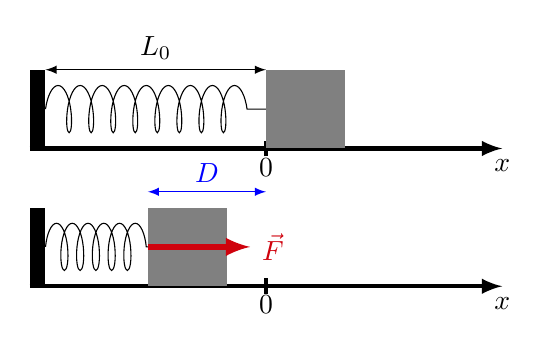
\begin{tikzpicture}[scale=1]
\tikzmath{
\L=2.;
\dx=0.75*\L;
\off=0.5;
\h=1;
}
\scalebox{1}{

\begin{scope}[shift={(0,1.75*\h)}]
\draw[-latex,line width=1.5pt] (-1.5*\L,0) -- (1.5*\L,0) node[below]{$x$};
\draw[line width=1.5pt] (0,-0.1) -- (0,0.1);
\node[below] at (0,0) {$0$};

\fill (-1.5*\L,0) rectangle (-1.4*\L,\h);
\draw[decoration={aspect=0.3, segment length=2.8mm, amplitude=3mm,coil},decorate] (-1.4*\L,\h/2) -- (0,\h/2);
\draw [latex-latex] (-1.4*\L,\h) -- (0,\h) node[midway,above]{$L_0$};
\fill[black!50] (0,0) rectangle (\h,\h);
\end{scope}
%%%%%%%%%%   compressed

\draw[-latex,line width=1.5pt] (-1.5*\L,0) -- (1.5*\L,0) node[below]{$x$};
\draw[line width=1.5pt] (0,-0.1) -- (0,0.1);
\node[below] at (0,0) {$0$};

\fill (-1.5*\L,0) rectangle (-1.4*\L,\h);
\draw[decoration={aspect=0.3, segment length=2mm, amplitude=3mm,coil},decorate] (-1.4*\L,\h/2) -- (-\dx,\h/2);
\draw [color=blue,latex-latex] (-\dx,1.2*\h) -- (0,1.2*\h) node[midway,above]{$D$};
\fill[black!50] (-\dx,0) rectangle (-\dx+\h,\h);
\draw[line width=2, -latex, color=myred] (-\dx,\h/2) -- +(1.3,0) node[right] {$\vec F$};

}
\end{tikzpicture}
\captionof*{figure}{\textit{Compressing a spring by a distance $D$.}}
\end{center}
}

%%%%%%%%%%%%%%%%%%%%%%%%%%%%%%%%
\twocolframe{Force varying with position (recap)}
{
\begin{itemize}
\item We can find the speed squared by applying the kinematic equation multiple times:
\begin{align*}
v_1^2&=v_0^2+2\frac{F_1}{m}\Delta x\\
v_n^2&=v_0^2+\frac{2}{m}\sum F_i\Delta x\\
\end{align*}
\item The velocity (squared) of the object as a function of position is given by:
\begin{align*}
v^2(x)=v_0^2+\frac{2}{m}\int F(x) dx
\end{align*}
\end{itemize}

}
{
\begin{center}
\begin{tikzpicture}[scale=1]
\tikzmath{
\L=10;
\h=0.75;
\w=0.2;
\dx=2.5;
\abox=0.75;
\Fm=1;
}
\scalebox{0.7}{
%axis
\draw[-latex, line width=1.5pt] (0,0) -- (\L,0) node[below]{$x$};
\draw[line width=1.5pt] (0,0.1) -- (0,-0.1) node[below]{$0$};
%floor
\fill[black!50] (0,\h) rectangle (\L,\h+\w);

\fill[color=myblue!60] (0.5*\dx,\h+\w) rectangle (0.5*\dx+\abox,\h+\w+\abox);
\fill[color=myblue!60] (1.5*\dx,\h+\w) rectangle (1.5*\dx+\abox,\h+\w+\abox);
\fill[color=myblue!60] (2.5*\dx,\h+\w) rectangle (2.5*\dx+\abox,\h+\w+\abox);

\draw[latex-,line width=2] (0.5*\dx,\h+\w+\abox/2) -- +(-\Fm,0) node[midway,above]{$\vec F_1$};
\draw[latex-,line width=2] (1.5*\dx,\h+\w+\abox/2) -- +(-1.25*\Fm,0) node[midway,above]{$\vec F_2$};
\draw[latex-,line width=2] (2.5*\dx,\h+\w+\abox/2) -- +(-1.5*\Fm,0) node[midway,above]{$\vec F_3$};

\draw[dotted, line width=1] (0.5*\dx,\h) -- +(0,-\h) node[below]{$x_1$};
\draw[dotted, line width=1] (1.5*\dx,\h) -- +(0,-\h) node[below]{$x_2$};
\draw[dotted, line width=1] (2.5*\dx,\h) -- +(0,-\h) node[below]{$x_3$};
\draw[dotted, line width=1] (3.5*\dx,\h) -- +(0,-\h) node[below]{$x_4$};

\draw[latex-latex, line width=1] (0.5*\dx,0.75*\h)--+(\dx,0) node[midway, below]{$\Delta x$};
\draw[latex-latex, line width=1] (1.5*\dx,0.75*\h)--+(\dx,0) node[midway, below]{$\Delta x$};
\draw[latex-latex, line width=1] (2.5*\dx,0.75*\h)--+(\dx,0) node[midway, below]{$\Delta x$};
}
\end{tikzpicture}
\captionof*{figure}{\textit{A block slides along $x$ with a force that changes depending on position}}
\end{center}
}


%%%%%%%%%%%%%%%%%%%%%%%%%%%%%%%%
\twocolframe{Force varying with position (recap)}
{
\begin{itemize}
\item A block is pushed against a spring, compressing it by a distance $D$. The force on the block (exerted by the spring) changes with position:
\begin{align*}
F(x)=-kx
\end{align*}
\item  Having released the block at rest ($v_0=0$) from $x = -D$, its speed when it reaches $x = 0$ is:
\begin{align*}
v^2(x=0)&=-\frac{2}{m}\int_{-D}^{0}kxdx=-\frac{2}{m}\left[\frac{1}{2}kx^2 \right]_{-D}^{0}\\
&=\frac{k}{m}D^2
\end{align*}
\end{itemize}

}
{
\begin{center}
\begin{tikzpicture}[scale=1]
\tikzmath{
\L=2.;
\dx=0.75*\L;
\off=0.5;
\h=1;
}
\scalebox{1}{

\begin{scope}[shift={(0,1.75*\h)}]
\draw[-latex,line width=1.5pt] (-1.5*\L,0) -- (1.5*\L,0) node[below]{$x$};
\draw[line width=1.5pt] (0,-0.1) -- (0,0.1);
\node[below] at (0,0) {$0$};

\fill (-1.5*\L,0) rectangle (-1.4*\L,\h);
\draw[decoration={aspect=0.3, segment length=2.8mm, amplitude=3mm,coil},decorate] (-1.4*\L,\h/2) -- (0,\h/2);
\draw [latex-latex] (-1.4*\L,\h) -- (0,\h) node[midway,above]{$L_0$};
\fill[black!50] (0,0) rectangle (\h,\h);
\end{scope}
%%%%%%%%%%   compressed

\draw[-latex,line width=1.5pt] (-1.5*\L,0) -- (1.5*\L,0) node[below]{$x$};
\draw[line width=1.5pt] (0,-0.1) -- (0,0.1);
\node[below] at (0,0) {$0$};

\fill (-1.5*\L,0) rectangle (-1.4*\L,\h);
\draw[decoration={aspect=0.3, segment length=2mm, amplitude=3mm,coil},decorate] (-1.4*\L,\h/2) -- (-\dx,\h/2);
\draw [color=blue,latex-latex] (-\dx,1.2*\h) -- (0,1.2*\h) node[midway,above]{$D$};
\fill[black!50] (-\dx,0) rectangle (-\dx+\h,\h);
\draw[line width=2, -latex, color=myred] (-\dx,\h/2) -- +(1.3,0) node[right] {$\vec F$};

}
\end{tikzpicture}
\captionof*{figure}{\textit{Compressing a spring by a distance $D$.}}
\end{center}
}
%%%%%%%%%%%%%%%%%%%%%%%










%%%%%%%%%%%%%%%%%%%%%%%%%%

\section{Mathmatical Applications}
\label{sec:mathmaticalapplications}
\title{Mathmatical Applications}
\institute{Applying Newton's Laws}
\author{\insertsubsection}


%%%%%%%%%%%%%%%%%%%%%%%%%
\begin{frame}
\titlepage
\thispagestyle{empty}
\end{frame}

%%%%%%%%%%%%%%%%%%%%







%%%%%%%%%%%%%%%%%%%%%%%%%%%%%%%%
\subsection{Derrivation for force varying with position}
\begin{frame}{Mathematically, more formally}
\begin{itemize}
\item<1-> We know acceleration as a function of position:
\begin{align*}
\frac{dv}{dt}=a(x)=\frac{F(x)}{m}
\end{align*}
\item<2-> We cannot integrate over $t$, since $x$ (the position of where the force is applied) depends on $t$:
\begin{align*}
dv=a(x)dt
\end{align*}
\item<3-> We need to integrate over $x$, and change variables from $t$ to $x$:
\begin{align*}
\frac{dx}{dt}=v\rightarrow dt=\frac{1}{v}dx
\end{align*}
\item<4-> We can thus write
\begin{align*}
dv=a(x)dt=\frac{a(x)}{v}dx
\end{align*}
\end{itemize}
\end{frame}

%%%%%%%%%%%%%%%%%%%%%%%%%%%%%%%%
\begin{frame}{Mathematically, more formally}
\begin{itemize}
\item<1-> Think of the Chain Rule for the same result:
\begin{align*}
\frac{dv}{dx}&=\frac{dv}{dt}\frac{dt}{dx}=a\frac{1}{v}\\
\therefore dv &=\frac{a}{v}dx
\end{align*}
\item<2-> This allows us to ``separate variables'':
\begin{align*}
vdv=a(x)dx
\end{align*}
\item<3-> We can ``add together'' things on the right and the left, and they must still be equal:
\begin{align*}
\int_{v_0}^{v(x_1)}vdv&=\int_{x_0}^{x_1} a(x)dx\\
\frac{1}{2}v^2(x)-\frac{1}{2}v_0^2&=\int_{x_0}^{x_1} a(x)dx\\
\therefore v^2(x)&=v_0^2+2\int_{x_0}^{x_1} a(x)dx=v_0^2+\frac{2}{m}\int_{x_0}^{x_1} F(x)dx
\end{align*}
\end{itemize}
\end{frame}


%%%%%%%%%%%%%%%%%%%%%%%%%%%%%%%%
\begin{frame}{Mathematically, more formally}
\begin{itemize}
\item With constant acceleration, this just gives the kinematics equation:
\begin{align*}
v^2(x_1)&=v_0^2+2\int_{x_0}^{x_1} a(x)dx\\
&=v_0^2+2a(x_1-x_0)
\end{align*}
\item This is also where kinetic energy comes from (next week!)
\begin{align*}
v^2(x_1)&=v_0^2+\frac{2}{m}\int_{x_0}^x F(x)dx\\
\therefore \frac{1}{2}mv^2(x_1)-\frac{1}{2}mv_0^2&=\int_{x_0}^x F(x)dx
\end{align*}
Final kinetic energy minus initial kinetic energy is equal to Work done...
\end{itemize}
\end{frame}


%%%%%%%%%%%%%%%%%%%%%%%%%%%%%%%%
\subsection{Differential equations}
\label{subsec:differentialequations}
\begin{frame}{Differential equations}
\begin{itemize}
\item This is a differential equation:
\begin{align*}
vdv=a(x)dx
\end{align*}
\item We could write it as:
\begin{align*}
\frac{dv}{dx}=\frac{a(x)}{v}
\end{align*}
\item The derivative of a function $\frac{dv}{dx}$ depends on the function ($v(x)$) itself.
\item It is a \textbf{separable differential} equation, because we can separate all that depends on $v$ and $x$ onto separate sides of the equation (as in the first line). This allows us to find $v(x)$ by integrating both sides, as in the last slides.
\item Separable = usually easy to solve.
\item At this point, \textbf{you're not expected to solve a differential equation}, but you should understand the concept and how we're solving a separable equation. 
\end{itemize}

\end{frame}


%%%%%%%%%%%%%%%%%%%%%%%%%%%%%%%%
\subsection{Force varying with velocity}
\label{subsec:forcevaryingwithvelocity}
\twocolframest{Force varying with velocity (e.g. drag)}
{
\begin{itemize}
\item The force of drag (aka air resistance) depends on velocity.
\item Ultimately, it depends on the actual situation, sometimes it depends on $v$, sometimes on $v^2$.
\item The force also depends on the medium through which the object moves, and the size of the object.
\item Can model this as:
\begin{align*}
\vec F_d&=-b\vec v\\
\vec F_d&=-bv^2\hat v\\
\end{align*}
\end{itemize}
}
{
\begin{center}
\begin{tikzpicture}[scale=1]
\tikzmath{
\L=2.;
\dx=0.75*\L;
\off=0.5;
\h=1;
}
\scalebox{1}{

\fill (0,0) circle (3pt);
\draw[-latex,line width=2] (0,0)--+(0,1.) node[right]{$\vec F_d$};
\draw[-latex,line width=2] (0,0)--+(0,-1.5) node[right]{$\vec F_g$};

\draw[-latex,line width=4] (1,0)--+(0,-1) node[midway,right]{$\vec a$};
\draw[-latex,line width=1] (-1,0)--+(0,-1) node[left]{$x$};
}
\end{tikzpicture}
\captionof*{figure}{\textit{A model for drag.}}
\end{center}
}


%%%%%%%%%%%%%%%%%%%%%%%%%%%%%%%%
\subsection{Example: linear drag force}
\twocolframe{Example: Drag linear with velocity}
{
\scriptsize
\begin{itemize}
\item We assume drag is linear (and write the $x$ component):
\begin{align*}
 F_d&=-b v\\
\end{align*}
\item<2-> Writing Newton's Second Law (which is a differential equation):
\begin{align*}
\sum F-x = mg-bv&=ma \\
mg-bv&= m\frac{dv}{dt}
\end{align*}
\item<3-> It's separable:
\begin{align*}
\frac{dv}{mg-bv}=-\frac{b}{m}dt
\end{align*}
\end{itemize}
}
{
\begin{center}
\begin{tikzpicture}[scale=1]
\tikzmath{
\L=2.;
\dx=0.75*\L;
\off=0.5;
\h=1;
}
\scalebox{1}{

\fill (0,0) circle (3pt);
\draw[-latex,line width=2] (0,0)--+(0,1.) node[right]{$\vec F_d$};
\draw[-latex,line width=2] (0,0)--+(0,-1.5) node[right]{$\vec F_g$};

\draw[-latex,line width=4] (1,0)--+(0,-1) node[midway,right]{$\vec a$};
\draw[-latex,line width=1] (-1,0)--+(0,-1) node[left]{$x$};
}
\end{tikzpicture}
\captionof*{figure}{\textit{A model for drag.}}
\end{center}
}


%%%%%%%%%%%%%%%%%%%%%%%%%%%%%%%%
\twocolframe{Example: Drag linear with velocity}
{
\begin{itemize}
\item<1-> So we can integrate both sides:
\begin{align*}
\int_0^{v(t_1)}\frac{dv}{mg-bv}dv=-\int_0^{t_1}\frac{b}{m}dt
\end{align*}
\item<2-> to find (after some math):
\begin{align*}
v(t_1)=\frac{mg}{b}\left(1-e^{-\frac{b}{m}t_1}\right)
\end{align*}
\end{itemize}
\only<2>{The speed increases asymptotically to the ``terminal velocity''. In the limit $t\to\infty$, we have:
\begin{align*}
v(t\to \infty) = \frac{mg}{b}
\end{align*}
}
}
{
\only<2>{
%\capfig{1}{figures/vterminal}{In the limit of $t\to\infty$, we have $v(t)=\frac{mg}{b}$, the object reaches ``terminal velocity''. This corresponds to the force of drag increasing until it reaches the magnitude of the force of gravity.}
\vspace{-1.5cm}
\begin{center}
 \begin{tikzpicture}
 \tikzmath{
 \ma=10;
 \b=0.5;
 }
 \scalebox{0.75}{
 \begin{axis}[domain = 0:100, grid,legend pos=south east,xlabel=$t$ (s), ylabel=$v(t)$ (m/s)]
  \addplot[smooth,color=blue,line width=2] {(\ma*9.81/\b)*(1-exp(-\b/\ma*x)};
  \addplot[smooth,dashed,color=myred,line width=2] {\ma*9.81/\b};

  \addlegendentry{$v(t)$}
  \addlegendentry{$v_{term}$}


 \end{axis}

 }
 \end{tikzpicture}
 \captionof*{figure}{\textit{Speed as a function of time for an object that started from rest and falls with drag. The object has a mass of $m=\SI{10}{kg}$ and the coefficient of drag is given by $b=\SI{0.5}{N\cdot s/m}$}.}
\end{center}


}
\only<1>{

\begin{center}
\begin{tikzpicture}[scale=1]
\tikzmath{
\L=2.;
\dx=0.75*\L;
\off=0.5;
\h=1;
}
\scalebox{1}{

\fill (0,0) circle (3pt);
\draw[-latex,line width=2] (0,0)--+(0,1.) node[right]{$\vec F_d$};
\draw[-latex,line width=2] (0,0)--+(0,-1.5) node[right]{$\vec F_g$};

\draw[-latex,line width=4] (1,0)--+(0,-1) node[midway,right]{$\vec a$};
\draw[-latex,line width=1] (-1,0)--+(0,-1) node[left]{$x$};
}
\end{tikzpicture}
\captionof*{figure}{\textit{A model for drag.}}
\end{center}
}
}






%%%%%%%%%%%%%%%%%%%%%%%%%%%%%%%%

\section{Building Models}
\label{sec:buildingmodelsnl}
\title{Building Models Using Newton's Laws}
\institute{Applying Newton's Laws}
\author{\insertsubsection}


%%%%%%%%%%%%%%%%%%%%%%%%%
\begin{frame}
\titlepage
\thispagestyle{empty}
\end{frame}


%%%%%%%%%%%%%%%%%%%%%%%%%%%%%%%%











%%%%%%%%%%%%%%%%%%%%%%%%%%%%%%%%
\subsection{Applying Newton's Laws}
\label{subsec:applyingnewtonslaws}
\twocolframesf{Reminder: Applying Newton's Laws}
{\scriptsize
Strongly recommend the following procedure for model building:
\begin{enumerate}
\item \textbf{Make a very good Free Body Diagram} for each mass that shows:
\begin{enumerate}
\scriptsize
\item All the forces (``what could be pushing or pulling on the mass?'').
\item The acceleration vector.
\item Relevant angles.
\item Your choice of coordinate system (make $+x$ parallel to acceleration).
\end{enumerate}
\item Read off the free-body diagram(s) to write Newton's Second Law, you get one equation per dimension:
\begin{align*}
\sum F_x = ma \quad \sum F_y=0
\end{align*}
 (if you chose x-axis parallel to acceleration, not always possible).
\item You now have a series of equations, just do some math to solve for any variables you need.
\end{enumerate}

}
{
\vspace{-1cm}
\begin{center}
\begin{tikzpicture}[scale=1]
\tikzmath{
\th=30;
\no=1.5;
\vg=cos(\th)*\no;
\fk=0.75;
}
\pgfmathsetmacro{\T}{1}
\scalebox{1}{
\coordinate (P) at (0,0);

\fill (P) circle(3pt);
\draw[-latex, line width=2] (P) -- (0,-\vg) node[right]{$\vec F_g$};
\draw[-latex, line width=2] (P) -- (90-\th:\no) node[right]{$\vec N$};
\draw[-latex, line width=2] (P) -- (180-\th:\T) node[above]{$\vec T$};
\draw[-latex, line width=2] (P) -- (-\th:\fk) node[above]{$\vec f_k$};

\draw[dotted, line width=1] (P) -- +(0,\vg);
\draw ($(P)+(0,0.5)$) arc(90:90-\th:0.5) node[midway,above]{$\theta$};

\draw[dotted, line width=1] (P) -- +(-\T,0);
\draw ($(P)+(-0.5,0)$) arc(180:180-\th:0.5) node[midway,left]{$\theta$};


\draw[-latex, line width=1] ($(P)+(-0.5,1.25)$) -- +(180-\th:1) node[below]{$\vec x$};
\draw[-latex, line width=1] ($(P)+(-0.5,1.25)$) -- +(90-\th:1) node[right]{$\vec y$};
\draw[-latex, line width=5] ($(P)+(-1.25,0)$) -- +(180-\th:1) node[midway,above]{$\vec a$};

}
\end{tikzpicture}
\captionof*{figure}{\textit{Reading off your very good free body diagram}}
\end{center}
\scriptsize
Reading off the diagram to write Newton's Second Law:
\begin{align*}
\sum F_x&: &T-f_k-F_g\sin\theta &= ma \\
\sum F_y&: &N-F_g\cos\theta &=0
\end{align*}
}


%%%%%%%%%%%%%%%%%%%%%%%%%%%%%%%%
\subsection{Circular motion with Newton's laws}
\label{subsec:circularmotionwithnewtonslaws}
\begin{frame}{Newton’s Laws and Circular motion}
\begin{itemize}
\item In circular motion (motion along a circle):
\begin{itemize}
\item The velocity is always tangent to the circle.
\item \textbf{There is always a centripetal component of acceleration} (radial acceleration, perpendicular to the velocity, responsible for changing the direction of $\vec v$).
\item There can be a tangential component of the acceleration, if the object changes speed (\textbf{non-uniform} circular motion).
\item The angular quantities ($\theta,\omega,\alpha$) are related to the tangential quantities (e.g. $v=\omega R$, $a_T=\alpha R$ ).
\end{itemize}
\item The sum of the forces must be parallel to the total acceleration:
\begin{align*}
\sum \vec F=m\vec a
\end{align*}
\item Can break this up into radial and tangential components (a good choice of $xy$):
\begin{align*}
\sum F_R&=ma_R=m\frac{v^2}{R}=m\omega^2R\quad \text{(Radial component, never zero)}\\
\sum F_T&=ma_T=m\alpha R\quad \text{(Tangential component, zero if uniform circ. mot.)}
\end{align*}
\end{itemize}
\end{frame}



%%%%%%%%%%%%%%%%%%%%%%%%%%%%%%%%
\subsection{Two masses on accelerating turntable}
\label{subsec:twomassesonacceleratingturntable}
\twocolframesf{Two masses on accelerating turntable}
{\scriptsize
\begin{itemize}
\item Both tangential and radial acceleration, only force of static friction can result in acceleration.
\item Both masses have the same angular velocity ($\omega$) and angular acceleration ($\alpha$).
\item Masses stay while $f_s\leq \mu_sN=\mu_smg$.
\item Tangential (linear) acceleration (constant):
\begin{align*}
ma_T=m\alpha r=f_{sT}
\end{align*}
\item Radial (linear) acceleration (increasing):
\begin{align*}
ma_R=m\omega^2r=f_{sR}
\end{align*}
\item Magnitude of the force of friction:
\begin{align*}
f_s=\sqrt{f_{sT}^2+f_{sR}^2}=mr\sqrt{\alpha^2+\omega^2}\leq mg\\
\therefore r\sqrt{\alpha^2+\omega^2}\leq g
\end{align*}
\end{itemize}
}
{
\begin{center}
\begin{tikzpicture}[scale=1]
\tikzmath{
\R=2;
\th=30;
\fss=1.25;
\fst=\fss*cos(\th);
\fsr=-\fss*sin(\th);
}
\scalebox{1}{
\coordinate (C) at (0,0);

\fill[myblue!40] (C) circle(\R);
\fill[] ($(C)+(0.25*\R,0)$) circle(5pt);
\fill[] ($(C)+(0.75*\R,0)$) circle(5pt);
\node[below=10pt] at ($(C)+(0.25*\R,0)$) {$m$};
\node[below=10pt] at ($(C)+(0.75*\R,0)$) {$M$};

\draw[-latex, line width=2] ($(C)+(0.25*\R,0)$) --+(\fsr,\fst) node[above]{$\vec f_s$};
\draw[-latex,dotted, line width=2] ($(C)+(0.25*\R,0)$) --+(\fsr,0) node[below]{$\vec f_{sR}$};
\draw[-latex,dotted, line width=2] ($(C)+(0.25*\R,0)$) --+(0,\fst) node[right]{$\vec f_{sT}$};

\draw[-latex, line width=2] (1.1*\R,0) arc (0:45:1.1*\R);
}
\end{tikzpicture}
\captionof*{figure}{\textit{Two masses on an accelerating turntable.}}
\end{center}
\only<2>{
\textcolor{myred}{Since $\alpha$ and $\omega$ are the same for both masses, the one with the larger value of $r$ will fall of first, regardless of mass!}
}
}

%%%%%%%%%%%%%%%%%%%%%%%%%%%%%%%%


%%%%%%%%%%%%%%%%%%%%%%%%%%%%%%%%
\subsection{Uniform circular motion}
\label{subsec:uniformcircularmotion}
\twocolframesf{Modeling \textit{uniform} circular motion}
{
\begin{itemize}
\item Uniform means constant speed (no tangential acceleration).
\item The \textbf{net acceleration} is towards the centre of the circle:
\begin{align*}
a_C=a_R=m\frac{v^2}{R}
\end{align*}
\item The \textbf{sum of the forces} is directed towards the centre of the circle:
\begin{align*}
\sum F_R&=m\frac{v^2}{R}\\
\sum F_T&=0\\
\end{align*}
\end{itemize}
}
{

 \begin{tikzpicture}[scale=1]
 \scalebox{1}{
  \coordinate (P1) at (-3,0);
  \node at (0,0) {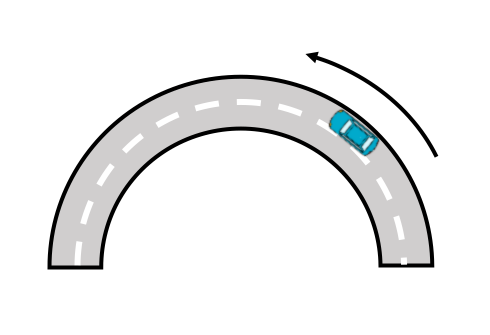
\includegraphics[scale=0.3]{figures/ApplyingNewtonsLaws/car2.png}};
  \fill[] (0,-1) circle(2pt);
  \draw[dotted,line width=1](0,-1) -- +(50:1.8)node[midway,below]{$R$}; 
 }
\end{tikzpicture}
\captionof*{figure}{\textit{Top view of car going around a corner}}
}


%%%%%%%%%%%%%%%%%%%%%%%%%%%%%%%%

%%%%%%%%%%%%%%%%%%%%%%%%%%%%%%%%
\subsection{Banked curves}
\label{subsec:bankedcurves}
\begin{frame}{Banked curves}
\begin{itemize}
\item By banking the road, one can change the direction of the normal force so that it, too, can have a component towards the centre of the circle
\end{itemize}
\begin{columns}[]

 \column{0.5\textwidth}
 \vspace{0.7cm}
 \begin{tikzpicture}[scale=1]
 \scalebox{1}{
  \coordinate (P1) at (-3,0);
  \node at (0,0) {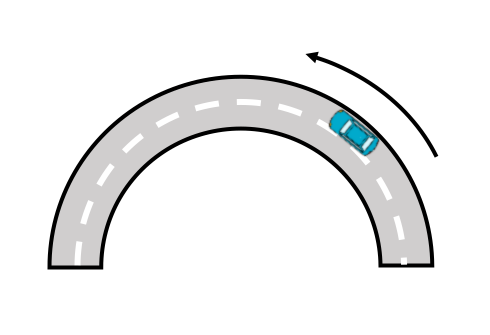
\includegraphics[scale=0.3]{figures/ApplyingNewtonsLaws/car2.png}};
  \fill[] (0,-1) circle(2pt);
  \draw[dotted,line width=1](0,-1) -- +(50:1.8)node[midway,below]{$R$}; 
 }
\end{tikzpicture}
\captionof*{figure}{\textit{Top view of car going around a corner}}
 
\column{0.5\textwidth}
 
\begin{tikzpicture}[scale=1]
\tikzmath{
\L=4;
\h=1.3;
\no=1.75;
\th=atan(\h/\L);
\nox=\no*sin(\th);
\noy=\no*cos(\th);
}
 \scalebox{1}{
  \coordinate (P1) at (1.75,1.15);
  \coordinate (P2) at ($(P1)+(0,1.5)$);
  
  \draw[line width=2] (\L,\h) -- (\L,0) -- (0,0) --cycle;
  
  \node at (P1) {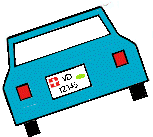
\includegraphics[scale=0.3]{figures/ApplyingNewtonsLaws/tiltedcar.png}};
  \draw (1,0) arc (0:\th:1) node[midway,right]{$\theta$};
  
  \draw[line width=1.5, dotted] (-1.5,1.15) -- (1.6, 1.15) node[midway,above]{$R$};
  
  \fill (P2) circle(3pt);
  \draw[line width=2,-latex] (P2) -- +(90+\th:\no) node[right]{$\vec N$};
  \draw[line width=1.5,-latex,color=myred] (P2) -- +(-\nox,0) node[midway,below] {$N\sin\theta$};
  \draw[dotted, line width=1] ($(P2)+(-\nox,0)$) -- +(0,\noy) node[midway,right=-3pt] {$\theta$};
 }
\end{tikzpicture}
\captionof*{figure}{\textit{Side view of car going around a banked curve.}}
 
\end{columns}
\end{frame}


%%%%%%%%%%%%%%%%%%%%%%%%%%%%%%%%


%%%%%%%%%%%%%%%%%%%%%%%%%%%%%%%%


%%%%%%%%%%%%%%%%%%%%%%%%%%%%%%%%
\subsection{Vertical Circle}
\label{subsec:verticalcircle}
\twocolframesf{Motion in a vertical circle}
{\begin{itemize}
\item What you did as an experiment in RA5.
\item A ball swinging around a rope, with a force of tension.
\item A roller coaster, with a normal force instead of tension. 
\end{itemize}
\textit{It can never be uniform circular motion, there will always be a tangential component to acceleration from gravity (except at the top and bottom).}
}
{
\begin{center}
\begin{tikzpicture}[scale=1]
\tikzmath{
\R=2;
\vg=1;
\t=1.25*\vg;
\tt=\vg;
\ttt=0.75*\vg;
}
\scalebox{1}{
\coordinate (C) at (0,0);
\coordinate (P1) at (0,-\R);
\coordinate (P2) at (\R,0);
\coordinate (P3) at (0,\R);


\draw (C) circle(\R);

\fill (P1) circle(3pt);
\fill (P2) circle(3pt);
\fill (P3) circle(3pt);

\draw[-latex, line width=2] (P1) -- +(0,-\vg) node[right]{$\vec F_g$};
\draw[-latex, line width=2] (P1) -- +(0,\t) node[right]{$\vec T_1$};

\draw[-latex, line width=2] (P2) -- +(0,-\vg) node[right]{$\vec F_g$};
\draw[-latex, line width=2] (P2) -- +(-\tt,0) node[above]{$\vec T_2$};
\draw[-latex, line width=2,color=myred] (P2) -- +(-\tt,-\vg) node[below]{$\sum \vec F$};

\draw[-latex, line width=2] (P3) -- +(0,-\vg) node[right]{$\vec F_g$};
\draw[-latex, line width=2] (P3) -- +(0,-\ttt) node[left]{$\vec T_3$};
}
\end{tikzpicture}
\captionof*{figure}{\textit{A mass on a string going around in a vertical circle. The sum of the forces only points to the centre of the circle at the top and bottom.}}
\end{center}
}


%%%%%%%%%%%%%%%%%%%%%%%%%%%%%%%%







































%%%%%%%%%%%%%%%%%%%%%%%%%%%%%%%%

\title{Work \& Energy}
\subject{Work, Work in nD and The Work-Energy Theorem}
\subtitle{Building Models to Describe our World}


%%%%%%%%%%%%%%%%%%%%%%%%%
%%%%%% Title slide %%%%%%
%%%%%%%%%%%%%%%%%%%%%%%%%
\chaptertitle{Work \& Energy}
\begin{frame}
\label{chap:workenergy}
\titlepage
\thispagestyle{empty}

\begin{textblock*}{5cm}(11cm,4cm)
    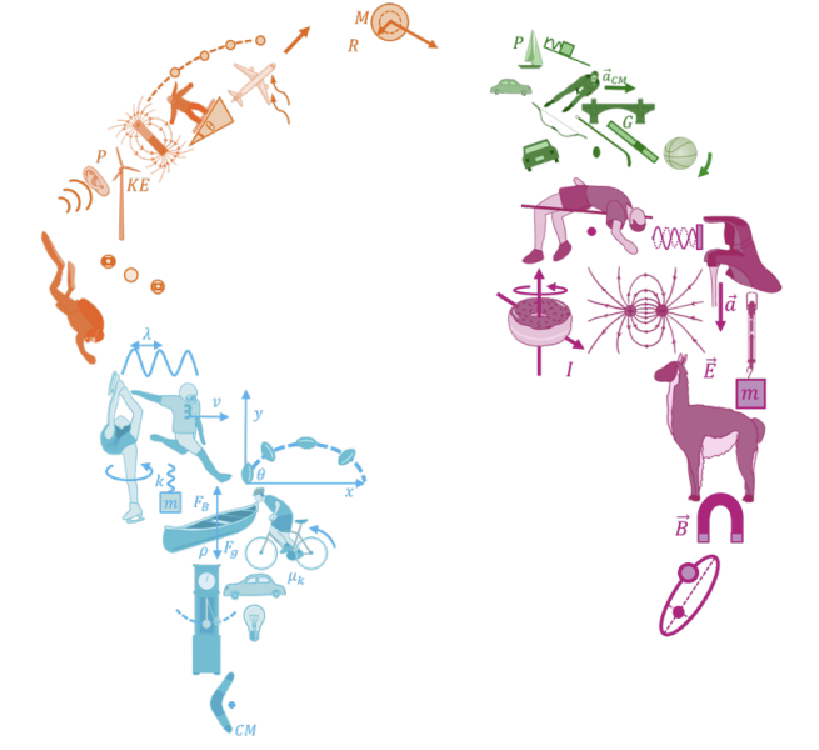
\includegraphics[width=4cm]{figures/BMDW/logo}
\end{textblock*}

\end{frame}

%%%%%%%%%%%%%%%%%%%%%%%%%%%%%

\twocolframe{Outline}
{\tableofcontents[sections=16-17, subsectionstyle=show/show]\thispagestyle{empty}}
{\tableofcontents[sections=18, subsectionstyle=show/show]}


%%%%%%%%%%%%%%%%%





\section{Introduction to Work}
\label{sec:introtowork}
\title{Introduction to Work}
\institute{Work \& Energy}
\author{\insertsubsection}


%%%%%%%%%%%%%%%%%%%%%%%%%
\begin{frame}
\titlepage
\thispagestyle{empty}
\end{frame}






%%%%%%%%%%%%%%%%%%%%%%%%%%%%%
\subsection{What is work?}
\label{subsec:whatiswork}
\begin{bulletframe}{Work}
\item The work ``done'' by a force, $\vec F$, over a displacement, $\vec d$, is defined to be:
\begin{align*}
W=\vec F\cdot \vec d=F_xd_x+F_yd_y+F_zd_z=Fd\cos\theta
\end{align*}
\item It is a useful quantity to connect the effect that a force has on changing the speed of an object:
\begin{itemize}
  \item[$\rightarrow$] Connecting dynamics (forces) to kinematics (change in speed).
\end{itemize}
 
\end{bulletframe}
%%%%%%%%%%%%%%%%%%%%%%%%%%%%%%%%



%%%%%%%%%%%%%%%%%%%%%%%%%%%%%%%%
\subsection{Work as a scalar product}
\label{subsec:workasascalarproduct}
\twocolframesf{Work as a scalar product}
{
\begin{itemize}
\item Think of it as a measure of whether the force is contributing to changing the speed of the object.
\item Only the component of the force parallel to the displacement can change its speed.
\item The scalar product ``picks out'' that component of the force: $F_\parallel=F\cos\theta$, $d_\parallel=d\cos\theta$.
\item Note that the \textit{component of the force perpendicular to the displacement can change the direction of the velocity}, but not the speed.
\begin{align*}
\vec F\cdot \vec d=Fd\cos\theta=F_\parallel d=F d_\parallel
\end{align*}
\end{itemize}
}
{
\begin{center}
\begin{tikzpicture}[scale=1]
\tikzmath{
\L=5;
\h=0.75;
\w=0.2;
\dx=2.5;
\abox=1.25;
\th=30;
\Fm=1.5;
\Fmx=\Fm*cos(\th);
\vdx=\dx*cos(\th);
}
\scalebox{1.0}{
%axis
\draw[-latex, line width=1.5pt] (0,0) -- (\L,0) node[below]{$x$};
\draw[line width=1.5pt] (0,0.1) -- (0,-0.1) node[below]{$0$};
%floor
\fill[black!50] (0,\h) rectangle (\L,\h+\w);

\fill[color=myblue!60] (0.5*\dx,\h+\w) rectangle (0.5*\dx+\abox,\h+\w+\abox);


\draw[-latex,line width=2] (0.5*\dx+\abox,\h+\w+\abox/2) -- +(\th:\Fm) node[midway,above]{$\vec F$};
\draw[dotted,line width=1] (0.5*\dx+\abox,\h+\w+\abox/2) -- +(0:1.25*\Fm);
\draw[-latex,dotted,line width=1] (0.5*\dx+\abox,\h+\w+\abox/2) -- +(\Fmx,0) node[below=-2pt]{$\vec F_{\parallel}$};
\draw (0.5*\dx+\abox+0.75,\h+\w+\abox/2) arc(0:\th:0.75)node[midway,right]{$\theta$};

\draw[-latex,line width=2] (0.5*\dx,\h+\w+2*\abox) -- +(\dx,0) node[midway,below]{$\vec d$};
\draw[-latex,dotted,line width=1] (0.5*\dx,\h+\w+2*\abox) -- +(\th:\vdx) node[midway,above]{$\vec d_{\parallel}$};
\draw[-latex,dotted,line width=1] ($(0.5*\dx,\h+\w+2*\abox)+(\th:\vdx)$) -- (1.5*\dx,\h+\w + 2*\abox)  node[midway,right]{$\vec d_{\perp}$}; ;
\draw (0.5*\dx+0.75,\h+\w+2*\abox) arc(0:\th:0.75)node[midway,right]{$\theta$};

\draw[dotted, line width=1] (0.5*\dx,\h) -- +(0,-\h) node[below]{$x_1$};
\draw[dotted, line width=1] (1.5*\dx,\h) -- +(0,-\h) node[below]{$x_2$};

\draw[latex-latex, line width=1] (0.5*\dx,0.75*\h)--+(\dx,0) node[midway, below]{$\Delta x$};

}
\end{tikzpicture}
\captionof*{figure}{\textit{A constant force, $\vec F$, does work on the block over the displacement vector, $\vec d$.}}
\end{center}
}


%%%%%%%%%%%%%%%%%%%%%%%%%%%%%%%%


%%%%%%%%%%%%%%%%%%%%%%%%%%%%%%%%
\subsection{Work with non-constant force: 1D}
\label{subsec:workwithnonconstantforce1d}
\twocolframe{Modeling work done by a non-constant force (1D)}
{
\begin{itemize}
\item Use the component of force parallel to displacement.
\item Divide the path up into segments where the force is (almost) constant.
\item Add up the work done on each segment:
\begin{align*}
W=F_1\Delta x+ F_2\Delta x+ F_3\Delta x+\dots
\end{align*}
\item<2-> If the force changes continuously, $F(x)$, need to sum infinitesimally small segments:
\begin{align*}
W=\lim_{\Delta x \to 0}\sum F_i\Delta x=\int_{x_1}^{x_f}F(x) dx
\end{align*}
\end{itemize}

}
{
\only<1-3>{
\vspace{-1cm}
\begin{center}
\begin{tikzpicture}[scale=1]
\tikzmath{
\L=10;
\h=0.75;
\w=0.2;
\dx=2.5;
\abox=0.75;
\Fm=1;
}
\scalebox{0.7}{
%axis
\draw[-latex, line width=1.5pt] (0,0) -- (\L,0) node[below]{$x$};
\draw[line width=1.5pt] (0,0.1) -- (0,-0.1) node[below]{$0$};
%floor
\fill[black!50] (0,\h) rectangle (\L,\h+\w);

\fill[color=myblue!60] (0.5*\dx,\h+\w) rectangle (0.5*\dx+\abox,\h+\w+\abox);
\fill[color=myblue!60] (1.5*\dx,\h+\w) rectangle (1.5*\dx+\abox,\h+\w+\abox);
\fill[color=myblue!60] (2.5*\dx,\h+\w) rectangle (2.5*\dx+\abox,\h+\w+\abox);

\draw[-latex,line width=2] (0.5*\dx,\h+\w+2*\abox) -- +(\dx,0) node[midway,below]{$\vec d$};

\draw[latex-,line width=2] (0.5*\dx,\h+\w+\abox/2) -- +(-\Fm,0) node[midway,above]{$\vec F_1$};
\draw[latex-,line width=2] (1.5*\dx,\h+\w+\abox/2) -- +(-1.25*\Fm,0) node[midway,above]{$\vec F_2$};
\draw[latex-,line width=2] (2.5*\dx,\h+\w+\abox/2) -- +(-1.5*\Fm,0) node[midway,above]{$\vec F_3$};

\draw[dotted, line width=1] (0.5*\dx,\h) -- +(0,-\h) node[below]{$x_1$};
\draw[dotted, line width=1] (1.5*\dx,\h) -- +(0,-\h) node[below]{$x_2$};
\draw[dotted, line width=1] (2.5*\dx,\h) -- +(0,-\h) node[below]{$x_3$};
\draw[dotted, line width=1] (3.5*\dx,\h) -- +(0,-\h) node[below]{$x_4$};

\draw[latex-latex, line width=1] (0.5*\dx,0.75*\h)--+(\dx,0) node[midway, below]{$\Delta x$};
\draw[latex-latex, line width=1] (1.5*\dx,0.75*\h)--+(\dx,0) node[midway, below]{$\Delta x$};
\draw[latex-latex, line width=1] (2.5*\dx,0.75*\h)--+(\dx,0) node[midway, below]{$\Delta x$};
}
\end{tikzpicture}
\captionof*{figure}{\textit{A block slides along $x$ with a force that depends on position.}}
\end{center}}
\only<3>{
\scriptsize
If $F(x)=\text{constant}$:
\begin{align*}
W=\int_{x_1}^{x_f}F(x) dx=F\int_{x_1}^{x_f} dx=F(x_f-x_1)
\end{align*}
$(x_f-x_1)$ is just the total displacement.
}

\only<4->{
\vspace{-0.2cm}
\begin{center}
\begin{tikzpicture}[scale=1]
\tikzmath{
\L=2.;
\dx=0.75*\L;
\off=0.5;
\h=0.75;
}
\scalebox{0.7}{

\begin{scope}[shift={(0,-2*\h)}]
\draw[-latex,line width=1.5pt] (-1.5*\L,0) -- (1.5*\L,0) node[below]{$x$};
\draw[line width=1.5pt] (0,-0.1) -- (0,0.1);
\node[below] at (0,0) {$0$};

\fill (-1.5*\L,0) rectangle (-1.4*\L,\h);
\draw[decoration={aspect=0.3, segment length=2.4mm, amplitude=2mm,coil},decorate] (-1.4*\L,\h/2) -- (0,\h/2);
%\draw [latex-latex] (-1.4*\L,\h) -- (0,\h) node[midway,above]{$L_0$};
\fill[color=myblue!60] (0,0) rectangle (\h,\h);
\draw [-latex, line width=2] (-\dx,1.1*\h) -- (0,1.1*\h) node[midway,above]{$\vec d$};
 \node[below] at (-\dx,0) {$-D$};
 \draw[line width=1.5pt] (-\dx,-0.1) -- (-\dx,0.1);
\end{scope}
%%%%%%%%%%   compressed

\draw[-latex,line width=1.5pt] (-1.5*\L,0) -- (1.5*\L,0) node[below]{$x$};
\draw[line width=1.5pt] (0,-0.1) -- (0,0.1);
\node[below] at (0,0) {$0$};

\fill (-1.5*\L,0) rectangle (-1.4*\L,\h);
\draw[decoration={aspect=0.3, segment length=1.1mm, amplitude=2mm,coil},decorate] (-1.4*\L,\h/2) -- (-\dx,\h/2);

\fill[color=myblue!60] (-\dx,0) rectangle (-\dx+\h,\h);
\draw[line width=2, -latex] (-\dx,\h/2) -- +(1.3,0) node[right] {$\vec F$};
\draw[dotted,line width=2] (-\dx,0) -- +(0,-2*\h);

}
\end{tikzpicture}
\vspace{-0.2cm}
\captionof*{figure}{\textit{A spring does \textbf{positive} work on a block over a total displacement, $\vec d$, from $x=-D$ to $x=0$. The spring force depends on position, $F(x)=-kx$.}}
\end{center}
}
\only<5>{
\scriptsize
\begin{align*}
W&=\int_{x_1}^{x_f}F(x) dx=\int_{-D}^0 (-kx)dx=\left[-\frac{1}{2}kx^2 \right]_{-D}^0\\
&=\frac{1}{2}kD^2\quad\text{}
\end{align*}
The work done by a spring over a distance, $D$.
}
}
%%%%%%%%%%%%%%%%%%%%%%%%%%%%%%%%





%%%%%%%%%%%%%%%%%%%%%%%%%%%%%%%

\section{Work in nD}
\label{sec:workinnd}
\title{Work in nD}
\institute{Work \& Energy}
\author{\insertsubsection}


%%%%%%%%%%%%%%%%%%%%%%%%%
\begin{frame}
\titlepage
\thispagestyle{empty}
\end{frame}

%%%%%%%%%%%%%%%%%%%%%%%%










%%%%%%%%%%%%%%%%%%%%%%%%%%%%%%%%
\subsection{1D vs nD}
\label{subsec:1dvsnd}
\twocolframesf{Work in ND}
{
\begin{itemize}
\item Defined work, a scalar quantity, as a first step towards using scalars to describe the world instead of vectors:
\begin{align*}
W=\vec F\cdot \vec d
\end{align*}
\item The work done by a force is a measure of how much that force contributes to changing the speed of an object.
\item In general, the displacement may not be one-dimensional:
\begin{align*}
W=\vec F \cdot \vec d_1+\vec F \cdot \vec d_2+\vec F \cdot \vec d_3+
\end{align*}
\end{itemize}
}
{\vspace{-1.5cm}
%%%%%%%%%%% block with force
\begin{center}
\begin{tikzpicture}[scale=1]
\tikzmath{
\L=5;
\h=0.75;
\w=0.2;
\dx=2.5;
\abox=0.75;
\th=30;
\Fm=1.5;
\Fmx=\Fm*cos(\th);
\vdx=\dx*cos(\th);
}
\scalebox{1.0}{
%axis
\draw[-latex, line width=1.5pt] (0,0) -- (\L,0) node[below]{$x$};
\draw[line width=1.5pt] (0,0.1) -- (0,-0.1) node[below]{$0$};
%floor
\fill[black!50] (0,\h) rectangle (\L,\h+\w);

\fill[color=myblue!60] (0.5*\dx,\h+\w) rectangle (0.5*\dx+\abox,\h+\w+\abox);


\draw[-latex,line width=2] (0.5*\dx+\abox,\h+\w+\abox/2) -- +(\th:\Fm) node[midway,above]{$\vec F$};
\draw[dotted,line width=1] (0.5*\dx+\abox,\h+\w+\abox/2) -- +(0:1.25*\Fm);
\draw[-latex,dotted,line width=1] (0.5*\dx+\abox,\h+\w+\abox/2) -- +(\Fmx,0) node[above=-2pt]{$\vec F_{\parallel}$};
\draw (0.5*\dx+\abox+0.75,\h+\w+\abox/2) arc(0:\th:0.75)node[midway,right]{$\theta$};

\draw[-latex,line width=2] (0.5*\dx,\h+\w+2*\abox) -- +(\dx,0) node[midway,above]{$\vec d$};
\draw[-latex,dotted,line width=1] (0.5*\dx,\h+\w+2*\abox) -- +(\th:\vdx) node[midway,above]{$\vec d_{\parallel}$};
\draw[-latex,dotted,line width=1] ($(0.5*\dx,\h+\w+2*\abox)+(\th:\vdx)$) -- (1.5*\dx,\h+\w + 2*\abox)  node[midway,right]{$\vec d_{\perp}$}; ;
\draw (0.5*\dx+0.75,\h+\w+2*\abox) arc(0:\th:0.75)node[midway,right]{$\theta$};

\draw[dotted, line width=1] (0.5*\dx,\h) -- +(0,-\h) node[below]{$x_1$};
\draw[dotted, line width=1] (1.5*\dx,\h) -- +(0,-\h) node[below]{$x_2$};

\draw[latex-latex, line width=1] (0.5*\dx,0.75*\h)--+(\dx,0) node[midway, below]{$\Delta x$};

}
\end{tikzpicture}
%\captionof*{figure}{\textit{A constant force, $\vec F$, does work on the block over the displacement vector, $\vec d$.}}
\end{center}

%%%%%%% top view of ND motion:
\begin{center}
\begin{tikzpicture}[scale=1]
\tikzmath{
\L=3;
}
\scalebox{1.0}{
%axis
\coordinate (P1) at (0.1*\L,0.1*\L);
\coordinate (P2) at (0.5*\L,0.25*\L);
\coordinate (P3) at (0.5*\L,0.75*\L);
\coordinate (P4) at (1*\L,1*\L);

\fill (P1) circle(3pt);
\fill (P4) circle(3pt);
\draw[-latex, line width=1.5pt] (0,0) -- (0,\L) node[left]{$y$};
\draw[-latex, line width=1.5pt] (0,0) -- (\L,0) node[below]{$x$};

\draw[-latex, line width=2.pt, color=myred] (0.5*\L,0.1*\L) -- +(1,0) node[midway,above]{$\vec F$};

\draw[-latex, line width=2.pt] (P1) node[above]{$A$} -- (P2) node[midway,above]{$\vec d_1$};
\draw[-latex, line width=2.pt] (P2) -- (P3)node[midway,right]{$\vec d_2$};
\draw[-latex, line width=2.pt] (P3) -- (P4)node[midway,below]{$\vec d_3$} node[above]{$B$};


}
\end{tikzpicture}
%\captionof*{figure}{\textit{A constant force, $\vec F$, does work on the block over the displacement vector, $\vec d$.}}
\end{center}
}


%%%%%%%%%%%%%%%%%%%%%%%%%%%%%%%%

%%%%%%%%%%%%%%%%%%%%%%%%%%%%%%%%
\twocolframe{Recall 1D case}
{
\begin{itemize}
\item When force changes as a function of position, we must break up the motion into infinitesimal segments and use an integral to calculate the work:
\begin{align*}
W=\lim_{\Delta x \to 0}\sum F_i\Delta x=\int_{x_1}^{x_f}F(x) dx
\end{align*}
\item The net work done by a force can depend on the path taken between $x_1$ and $x_f$:
\begin{itemize}
\item For friction, it matters.
\item For a spring force, it doesn't matter.

\end{itemize}

\end{itemize}
}
{
\vspace{-2cm}
%$%%%%%%%%%%%%%% block on a line
\begin{center}
\begin{tikzpicture}[scale=1]
\tikzmath{
\L=10;
\h=0.75;
\w=0.2;
\dx=2.5;
\abox=0.75;
\Fm=1;
}
\scalebox{0.7}{
%axis
\draw[-latex, line width=1.5pt] (0,0) -- (\L,0) node[below]{$x$};
\draw[line width=1.5pt] (0,0.1) -- (0,-0.1) node[below]{$0$};
%floor
\fill[black!50] (0,\h) rectangle (\L,\h+\w);

\fill[color=myblue!60] (0.5*\dx,\h+\w) rectangle (0.5*\dx+\abox,\h+\w+\abox);
\fill[color=myblue!60] (1.5*\dx,\h+\w) rectangle (1.5*\dx+\abox,\h+\w+\abox);
\fill[color=myblue!60] (2.5*\dx,\h+\w) rectangle (2.5*\dx+\abox,\h+\w+\abox);

\draw[-latex,line width=2] (0.5*\dx,\h+\w+2*\abox) -- +(\dx,0) node[midway,below]{$\vec d$};

\draw[latex-,line width=2] (0.5*\dx,\h+\w+\abox/2) -- +(-\Fm,0) node[midway,above]{$\vec F_1$};
\draw[latex-,line width=2] (1.5*\dx,\h+\w+\abox/2) -- +(-1.25*\Fm,0) node[midway,above]{$\vec F_2$};
\draw[latex-,line width=2] (2.5*\dx,\h+\w+\abox/2) -- +(-1.5*\Fm,0) node[midway,above]{$\vec F_3$};

\draw[dotted, line width=1] (0.5*\dx,\h) -- +(0,-\h) node[below]{$x_1$};
\draw[dotted, line width=1] (1.5*\dx,\h) -- +(0,-\h) node[below]{$x_2$};
\draw[dotted, line width=1] (2.5*\dx,\h) -- +(0,-\h) node[below]{$x_3$};
\draw[dotted, line width=1] (3.5*\dx,\h) -- +(0,-\h) node[below]{$x_4$};

\draw[latex-latex, line width=1] (0.5*\dx,0.75*\h)--+(\dx,0) node[midway, below]{$\Delta x$};
\draw[latex-latex, line width=1] (1.5*\dx,0.75*\h)--+(\dx,0) node[midway, below]{$\Delta x$};
\draw[latex-latex, line width=1] (2.5*\dx,0.75*\h)--+(\dx,0) node[midway, below]{$\Delta x$};
}
\end{tikzpicture}
\captionof*{figure}{\textit{A block slides along $x$ with a force that depends on position.}}
\end{center}
%%%%%%%%%%%%%%%% spring
\begin{center}
\begin{tikzpicture}[scale=1]
\tikzmath{
\L=2.;
\dx=0.75*\L;
\off=0.5;
\h=0.75;
}
\scalebox{0.7}{

\begin{scope}[shift={(0,-2*\h)}]
\draw[-latex,line width=1.5pt] (-1.5*\L,0) -- (1.5*\L,0) node[below]{$x$};
\draw[line width=1.5pt] (0,-0.1) -- (0,0.1);
\node[below] at (0,0) {$0$};

\fill (-1.5*\L,0) rectangle (-1.4*\L,\h);
\draw[decoration={aspect=0.3, segment length=2.4mm, amplitude=2mm,coil},decorate] (-1.4*\L,\h/2) -- (0,\h/2);
%\draw [latex-latex] (-1.4*\L,\h) -- (0,\h) node[midway,above]{$L_0$};
\fill[color=myblue!60] (0,0) rectangle (\h,\h);
\draw [-latex, line width=2] (-\dx,1.1*\h) -- (0,1.1*\h) node[midway,above]{$\vec d$};
 \node[below] at (-\dx,0) {$-D$};
 \draw[line width=1.5pt] (-\dx,-0.1) -- (-\dx,0.1);
\end{scope}
%%%%%%%%%%   compressed

\draw[-latex,line width=1.5pt] (-1.5*\L,0) -- (1.5*\L,0) node[below]{$x$};
\draw[line width=1.5pt] (0,-0.1) -- (0,0.1);
\node[below] at (0,0) {$0$};

\fill (-1.5*\L,0) rectangle (-1.4*\L,\h);
\draw[decoration={aspect=0.3, segment length=1.1mm, amplitude=2mm,coil},decorate] (-1.4*\L,\h/2) -- (-\dx,\h/2);

\fill[color=myblue!60] (-\dx,0) rectangle (-\dx+\h,\h);
\draw[line width=2, -latex] (-\dx,\h/2) -- +(1.3,0) node[right] {$\vec F$};
\draw[dotted,line width=2] (-\dx,0) -- +(0,-2*\h);

}
\end{tikzpicture}
\captionof*{figure}{\textit{A spring does positive work on a block over a total displacement, $\vec d$, from $x=-D$ to $x=0$.}}
\end{center}
}


%%%%%%%%%%%%%%%%%%%%%%%%%%%%%%%%
\twocolframesf{In multiple dimensions}
{
\begin{itemize}
\item Force can depend on position (x,y,z) $\rightarrow$ $\vec F=\vec F(\vec r)$, where $\vec r$, is the position of the object.
\item A infinitesimal segment is not necessarily parallel to the $x,y,z$ axis, use $d\vec l$.
\item We write work as:
\begin{align*}
W=\int_A^B \vec F(\vec r) \cdot d\vec l
\end{align*}
\item Where $d\vec l$ is an infinitesimal segment, tangent to the path
\end{itemize}
}
{
\begin{center}
\begin{tikzpicture}[%
%https://tex.stackexchange.com/questions/25928/how-to-draw-tangent-line-of-an-arbitrary-point-on-a-path-in-tikz
        tangent/.style={
        decoration={
            markings,% switch on markings
            mark=
                at position ####1
                with
                {
                    \coordinate (tangent point-\pgfkeysvalueof{/pgf/decoration/mark info/sequence number}) at (0pt,0pt);
                    \coordinate (tangent unit vector-\pgfkeysvalueof{/pgf/decoration/mark info/sequence number}) at (1,0pt);
                    \coordinate (tangent orthogonal unit vector-\pgfkeysvalueof{/pgf/decoration/mark info/sequence number}) at (0pt,1);
                }
        },
        postaction=decorate
    },
    use tangent/.style={
        shift=(tangent point-####1),
        x=(tangent unit vector-####1),
        y=(tangent orthogonal unit vector-####1)
    },
    use tangent/.default=1
    ]
\tikzmath{
}

\scalebox{1.0}{

 \coordinate (P1) at (0.2,0.5);
 \coordinate (P2) at (1.75,2); %used to make the path squiggly
 \coordinate (P3) at (3.75,2.5);
 \coordinate (P3x) at ($(0,0)!(P3)!(1,0)$);
 \coordinate (P1P3) at ($(P3)!(P1)!(P3x)$);
 
 \draw[-latex, line width=1.5pt] (0,0) -- (4.5,0) node[below]{$x$}; 
 \draw[-latex, line width=1.5pt] (0,0) -- (0,3) node[left]{$y$}; 
 
 \fill (P1) circle(2pt) node[above]{$A$};;
 \fill (P3) circle(2pt) node[above]{$B$};;
 
  
 %The path with tangent coordinates calculated
 \draw[tangent=0.25,tangent=0.45,tangent=0.65, tangent=0.85,  line width=1pt] (P1) to [out=10,in=190] (P2) to [out=10,in=260] (P3);
 
 \draw [myred, -latex, line width=1.5, use tangent=2] (0,0) -- (0.5,0) node[above]{$d\vec l$};
 \draw [ -latex, line width=1.5, use tangent=2] (0,0) -- +(-60:1) node[right]{$\vec F(\vec r)$}; 
 \draw [ -latex, line width=1.5, use tangent=1] (0,0) -- +(-80:0.75) node[below]{$\vec F(\vec r)$}; 
 \draw [ -latex, line width=1.5, use tangent=3] (0,0) -- +(60:1.25) node[above]{$\vec F(\vec r)$}; 
}
\end{tikzpicture}
\captionof*{figure}{\textit{A position-dependent force, $\vec F(\vec r)$, does work along an arbitrary path.}}
\end{center}
}


%%%%%%%%%%%%%%%%%%%%%%%%%%%%%%%%

%%%%%%%%%%%%%%%%%%%%%%%%%%%%%%%%
\subsection{Path integrals}
\label{subsec:pathinegrals}
\twocolframesf{Path integrals}
{
\begin{itemize}
\item In general, the value of the integral will depend on what path you take between points $A$ and $B$ (think friction doing work).
\item This is different than ``normal'' integrals which only depend on the end points (you just evaluate the anti-derivative at the end points).
\item There are some forces (i.e. some functions ) for which the work done ultimately does not depend on the path taken, like gravity, which we will discuss next week.
\item \textbf{In general, it does depend on the path, and it’s difficult to calculate! We want to avoid doing this integral if we can!}
\end{itemize}
}
{
\begin{center}
\begin{tikzpicture}[%
%https://tex.stackexchange.com/questions/25928/how-to-draw-tangent-line-of-an-arbitrary-point-on-a-path-in-tikz
        tangent/.style={
        decoration={
            markings,% switch on markings
            mark=
                at position ####1
                with
                {
                    \coordinate (tangent point-\pgfkeysvalueof{/pgf/decoration/mark info/sequence number}) at (0pt,0pt);
                    \coordinate (tangent unit vector-\pgfkeysvalueof{/pgf/decoration/mark info/sequence number}) at (1,0pt);
                    \coordinate (tangent orthogonal unit vector-\pgfkeysvalueof{/pgf/decoration/mark info/sequence number}) at (0pt,1);
                }
        },
        postaction=decorate
    },
    use tangent/.style={
        shift=(tangent point-####1),
        x=(tangent unit vector-####1),
        y=(tangent orthogonal unit vector-####1)
    },
    use tangent/.default=1
    ]
\tikzmath{
}

\scalebox{1.0}{

 \coordinate (P1) at (0.2,0.5);
 \coordinate (P2) at (1.75,2); %used to make the path squiggly
 \coordinate (P3) at (3.75,2.5);
 \coordinate (P3x) at ($(0,0)!(P3)!(1,0)$);
 \coordinate (P1P3) at ($(P3)!(P1)!(P3x)$);
 
 \draw[-latex, line width=1.5pt] (0,0) -- (4.5,0) node[below]{$x$}; 
 \draw[-latex, line width=1.5pt] (0,0) -- (0,3) node[left]{$y$}; 
 
 \fill (P1) circle(2pt) node[above]{$A$};;
 \fill (P3) circle(2pt) node[above]{$B$};;
 
  
 %The path with tangent coordinates calculated
 \draw[tangent=0.25,tangent=0.45,tangent=0.65, tangent=0.85,  line width=1pt] (P1) to [out=10,in=190] (P2) to [out=10,in=260] (P3);
 
 \draw [myred, -latex, line width=1.5, use tangent=2] (0,0) -- (0.5,0) node[above]{$d\vec l$};

}
\end{tikzpicture}
\captionof*{figure}{\textit{An arbitrary path over which we may need to calculate a path integral.}}
\end{center}
}

%%%%%%%%%%%%%%%%%%%%%%%%%%%%%%%%
\subsection{Work from gravity on a pendulum}
\label{subsec:workfromgravityonpendulum}
\twocolframesf{Example: Work done by gravity on pendulum}
{
\scriptsize
\begin{itemize}
\item We want the work done by gravity along the arc:
\begin{align*}
W=\int_A^B \vec F_g\cdot d\vec l
\end{align*}
\item<2-> At some angle, $\theta$:
\begin{align*}
d\vec l &= dl(\cos\theta\hat x-\sin\theta\hat y)\\
\vec F_g&=-mg\hat y\\
\therefore \vec F_g\cdot d\vec l &=mg\sin\theta dl
\end{align*}
\item<3-> Noting that $dl=-Ld\theta$ ($d\theta$ is in the direction of increasing $\theta$):
\begin{align*}
W&=\int_A^B \vec F_g\cdot d\vec l=\int_{\theta_0}^0-mg\sin\theta L d\theta=mgL(1-\cos\theta_0)\\
&=mgh
\end{align*}
\end{itemize}

}
{
\begin{center}
\begin{tikzpicture}[scale=1]
\tikzmath{
\L=3.;
\R=0.3;
\th=40;
\vg=1;
\Ly=\L*cos(\th);
}
\scalebox{1.0}{
%pendulum

\draw[line width = 1.5pt] (0,0) -- (270-\th:\L) node[midway,above]{$L$};
\fill[color=myblue!60] (270-\th:\L) circle(\R); 
\draw[-latex, line width= 2pt](270-\th:\L) --+(0,-\vg) node[left]{$\vec F_g$};

\draw[dotted, line width = 1.5pt] (0,0) -- (270:\L);
\draw[dotted, line width = 1.5pt] (270-\th:\L) arc (270-\th:270:\L);
\draw (270-\th:0.75) arc (270-\th:270:0.75) node[midway,below]{$\theta$};
\draw[dotted, line width = 1.5pt] (270-\th:\L) -- (0,-\Ly);
\draw[latex-latex] (0.2,-\L) -- (0.2,-\Ly) node[midway,right]{$h$};
\draw[-latex,color=myred, line width = 1.5pt] (270-\th:\L) -- +(-\th:0.75) node[below]{$d\vec l$};
}
\end{tikzpicture}
\captionof*{figure}{\textit{Gravity does work on a pendulum as it swings from $\theta=\theta_0$ to $\theta=0$. The force is constant along the path, but the path is not a straight line.}}
\end{center}

}


%%%%%%%%%%%%%%%%%%%%%%%%%%%%%%%%









%%%%%%%%%%%%%%%%%%%%%%%%%%%%%%%%

\section{Work-Energy Theorem}
\label{sec:workenergytheorem}
\title{Work-Energy Theorem}
\institute{Work \& Energy}
\author{\insertsubsection}


%%%%%%%%%%%%%%%%%%%%%%%%%
\begin{frame}
\titlepage
\thispagestyle{empty}
\end{frame}

%%%%%%%%%%%%%%%%%%%%%%%%%%%%%%%%














%%%%%%%%%%%%%%%%%%%%%%%%%%%%%%%%
\subsection{Net work}
\label{subsec:network}
\twocolframesf{Work, in general}
{
\begin{align*}
W=\int_A^B \vec F(\vec r)\cdot d\vec r
\end{align*}
\begin{itemize}
\item Force can change magnitude and direction depending on position, $\vec F(\vec r)$.
\item Need to define work as a ``path integral'', as it depends on the path taken.
\item For example, to calculate the work done by friction in moving a crate along the floor, we summed the work done on each segment (path 2):
\begin{align*}
W=\vec f_1\cdot \vec d_1+\vec f_2 \cdot \vec d_2
\end{align*}
\end{itemize}
}
{
\begin{center}
\begin{tikzpicture}[%
%https://tex.stackexchange.com/questions/25928/how-to-draw-tangent-line-of-an-arbitrary-point-on-a-path-in-tikz
        tangent/.style={
        decoration={
            markings,% switch on markings
            mark=
                at position ####1
                with
                {
                    \coordinate (tangent point-\pgfkeysvalueof{/pgf/decoration/mark info/sequence number}) at (0pt,0pt);
                    \coordinate (tangent unit vector-\pgfkeysvalueof{/pgf/decoration/mark info/sequence number}) at (1,0pt);
                    \coordinate (tangent orthogonal unit vector-\pgfkeysvalueof{/pgf/decoration/mark info/sequence number}) at (0pt,1);
                }
        },
        postaction=decorate
    },
    use tangent/.style={
        shift=(tangent point-####1),
        x=(tangent unit vector-####1),
        y=(tangent orthogonal unit vector-####1)
    },
    use tangent/.default=1
    ]
\tikzmath{
}

\scalebox{1.0}{

 \coordinate (P1) at (0.2,0.5);
 \coordinate (P2) at (1.75,2); %used to make the path squiggly
 \coordinate (P3) at (3.75,2.5);
 \coordinate (P3x) at ($(0,0)!(P3)!(1,0)$);
 \coordinate (P1P3) at ($(P3)!(P1)!(P3x)$);
 
 \draw[-latex, line width=1.5pt] (0,0) -- (4.5,0) node[below]{$x$}; 
 \draw[-latex, line width=1.5pt] (0,0) -- (0,3) node[left]{$y$}; 
 
 \fill (P1) circle(2pt) node[above]{$A$};;
 \fill (P3) circle(2pt) node[above]{$B$};;
 
  
 %The path with tangent coordinates calculated
 \draw[tangent=0.25,tangent=0.45,tangent=0.65, tangent=0.85,  line width=1pt] (P1) to [out=10,in=190] (P2) to [out=10,in=260] (P3);
 
 \draw [myred, -latex, line width=1.5, use tangent=2] (-0.25,0) -- (0.25,0) node[above]{$d\vec l$};
 %\draw [ -latex, line width=1.5, use tangent=2] (0,0) -- +(-60:1) node[right]{$\vec F(\vec r)$}; 
 \draw [ -latex, line width=1.5, use tangent=1] (0,0) -- +(-80:0.75) node[below]{$\vec F(\vec r)$}; 
 %\draw [ -latex, line width=1.5, use tangent=3] (0,0) -- +(60:1.25) node[above]{$\vec F(\vec r)$}; 
 
 \begin{scope}[shift={(0,-3.5)}]
 
 \coordinate (A) at (0.75,0.5);
 \coordinate (B) at (3.75,2.5);
 
 
 \draw[-latex, line width=1.5pt] (0,0) -- (4.5,0) node[below]{$x$}; 
 \draw[-latex, line width=1.5pt] (0,0) -- (0,3) node[left]{$y$}; 

 \fill (A) circle(2pt) node[right]{$A(x_A,y_A)$};
 \fill (B) circle(2pt) node[above]{$B(x_B,y_B)$};
 
 \draw[dashed, line width=1.5] (A)--(B) node[midway,right=5pt]{path 1};
 
 \draw[-latex, color=myred, line width=1.5pt] (A)-- +(0,2.0)node[midway,left]{$\vec d_1$} node[above]{path 2};
 \draw[latex-, color=myred, line width=1.5pt] (B)-- +(-3,0) node[midway,above]{$\vec d_2$};
 
 \draw[latex-, line width=3] (1,1) -- +(0,1) node[midway, right]{$\vec f_1$};
 \draw[-latex, line width=3] (2.5,2.25) -- +(-1,0) node[midway, below]{$\vec f_2$};
 
 
 \end{scope} 
 
}
\end{tikzpicture}
\captionof*{figure}{\textit{Work is a path integral.}}
\end{center}

}


%%%%%%%%%%%%%%%%%%%%%%%%%%%%%%%%


%%%%%%%%%%%%%%%%%%%%%%%%%%%%%%%%
\begin{frame}{Net work done}
\begin{itemize}
\item If multiple forces are exerted on an object, as it moves, they can each do work.
\item The net work done on the object is the sum of the work done by each force exerted on the object:
\begin{align*}
W^{net}=\vec F_1\cdot \vec d+\vec F_2 \cdot \vec d+\vec F_3 \cdot \vec d+\dots
\end{align*}
\item Very easy to show that this is equivalent to:
\begin{align*}
W^{net}=(\vec F_1+\vec F_2+\vec F_3+\dots)\cdot \vec d=\vec F^{net}\cdot \vec d
\end{align*}
\end{itemize}
That is, the net work done on the object is the same as the work done by the net force.
\end{frame}


%%%%%%%%%%%%%%%%%%%%%%%%%%%%%%%%


%%%%%%%%%%%%%%%%%%%%%%%%%%%%%%%%
\subsection{Work-energy theorem}
\label{subsec:workenergytheorem}
\twocolframesf{Work-Energy theorem}
{\scriptsize
\begin{itemize}
\item<1-> In general, the \textbf{net} work done on an object can be written as:
\begin{align*}
W^{net}=\int_A^B\vec F^{net}(\vec r) \cdot d\vec l
\end{align*}
\item<2-> Using Newton’s Second Law:
\begin{align*}
F^{net} &= m\vec a =m\frac{d\vec v}{dt}\\
W^{net} &=\int_A^B m\frac{d\vec v}{dt}\cdot d\vec l\\
\only<3->{
&=m\int_A^B \frac{d\vec v}{dt}\cdot d\vec l=m\int_A^B d\vec v\cdot \frac{d\vec l}{dt}\\
}
\only<4->{
&=m\int_A^B d\vec v\cdot \vec v=m\int_A^B v dv\\
}
\only<5->{
&=\frac{1}{2}mv^2_B-\frac{1}{2}mv_A^2
}
\end{align*}
\end{itemize}
}
{
\begin{center}
\begin{tikzpicture}[%
%https://tex.stackexchange.com/questions/25928/how-to-draw-tangent-line-of-an-arbitrary-point-on-a-path-in-tikz
        tangent/.style={
        decoration={
            markings,% switch on markings
            mark=
                at position ####1
                with
                {
                    \coordinate (tangent point-\pgfkeysvalueof{/pgf/decoration/mark info/sequence number}) at (0pt,0pt);
                    \coordinate (tangent unit vector-\pgfkeysvalueof{/pgf/decoration/mark info/sequence number}) at (1,0pt);
                    \coordinate (tangent orthogonal unit vector-\pgfkeysvalueof{/pgf/decoration/mark info/sequence number}) at (0pt,1);
                }
        },
        postaction=decorate
    },
    use tangent/.style={
        shift=(tangent point-####1),
        x=(tangent unit vector-####1),
        y=(tangent orthogonal unit vector-####1)
    },
    use tangent/.default=1
    ]
\tikzmath{
}

\scalebox{1}{

 \coordinate (P1) at (0.2,0.5);
 \coordinate (P2) at (1.75,2); %used to make the path squiggly
 \coordinate (P3) at (3.75,2.5);
 \coordinate (P3x) at ($(0,0)!(P3)!(1,0)$);
 \coordinate (P1P3) at ($(P3)!(P1)!(P3x)$);
 
 \draw[-latex, line width=1.5pt] (0,0) -- (4.5,0) node[below]{$x$}; 
 \draw[-latex, line width=1.5pt] (0,0) -- (0,3) node[left]{$y$}; 
 
 \fill (P1) circle(2pt) node[above]{$A$};;
 \fill (P3) circle(2pt) node[above]{$B$};;
 
  
 %The path with tangent coordinates calculated
 \draw[tangent=0.25,tangent=0.45,tangent=0.65, tangent=0.85,  line width=1pt] (P1) to [out=10,in=190] (P2) to [out=10,in=260] (P3);
 
 \draw [myred, -latex, line width=1.5, use tangent=2] (-0.25,0) -- (0.25,0) node[above]{$\vec v = \frac{d\vec l}{dt}$};

}
\end{tikzpicture}
\captionof*{figure}{\textit{Instantaneous velocity, $\vec v$ is parallel to displacement, $d\vec l$.}}
\end{center}

}


%%%%%%%%%%%%%%%%%%%%%%%%%%%%%%%%
\begin{frame}{Work-Energy Theorem}
\begin{itemize}
\item Introduce ``Kinetic energy'':
\begin{align*}
K(v)=\frac{1}{2}mv^2
\end{align*}
\item The net work done on an object is the change in kinetic energy (final – initial)
\begin{align*}
W^{net} = \Delta K = K_B-K_A
\end{align*}
\item Now, we have a way to build models using scalar quantities (next week, we’ll introduce potential energy as a way to calculate work without using force vectors or path integrals). Note the connection between dynamics ($W$) and kinematics ($K$), just like Newton's Second Law (not surprising, since this came from Newton's Second Law!).
\end{itemize}
\end{frame}


%%%%%%%%%%%%%%%%%%%%%%%%%%%%%%%%


%%%%%%%%%%%%%%%%%%%%%%%%%%%%%%%%
\subsection{Power}
\label{subsec:power}
\begin{frame}{Power}
\begin{itemize}
\item Power is the rate at which work is being done.
\item If a force does work, $\Delta W$, in an amount of time, $\Delta t$, it did work with an average power:
\begin{align*}
P=\frac{\Delta W}{\Delta t}
\end{align*}
\item If the work done changes as a function of time, then we take the limit of $\Delta t\to 0$ to get the instantaneous power:
\begin{align*}
P=\frac{d W}{d t}
\end{align*}
\item Power is the rate at which a force changes the kinetic energy of an object (if it is the only force doing work) $\rightarrow$ think of this as the rate at which (kinetic) energy is being ``given/removed'' to/from the object.
\end{itemize}
\end{frame}

%%%%%%%%%%%%%%%%%%%%%%%%%%%%%%%%




































%%%%%%%%%%%%%%%%%%%%%%%%%%%%%%%%

\title{Potential \& Conservation of Energy}
\subject{Conservation, Potential and Potential Uses}
\subtitle{Building Models to Describe our World}


%%%%%%%%%%%%%%%%%%%%%%%%%
%%%%%% Title slide %%%%%%
%%%%%%%%%%%%%%%%%%%%%%%%%
\chaptertitle{Potential \& Conservation of Energy}
\begin{frame}
\label{chap:potentialecon}
\titlepage
\thispagestyle{empty}

\begin{textblock*}{5cm}(11cm,4cm)
    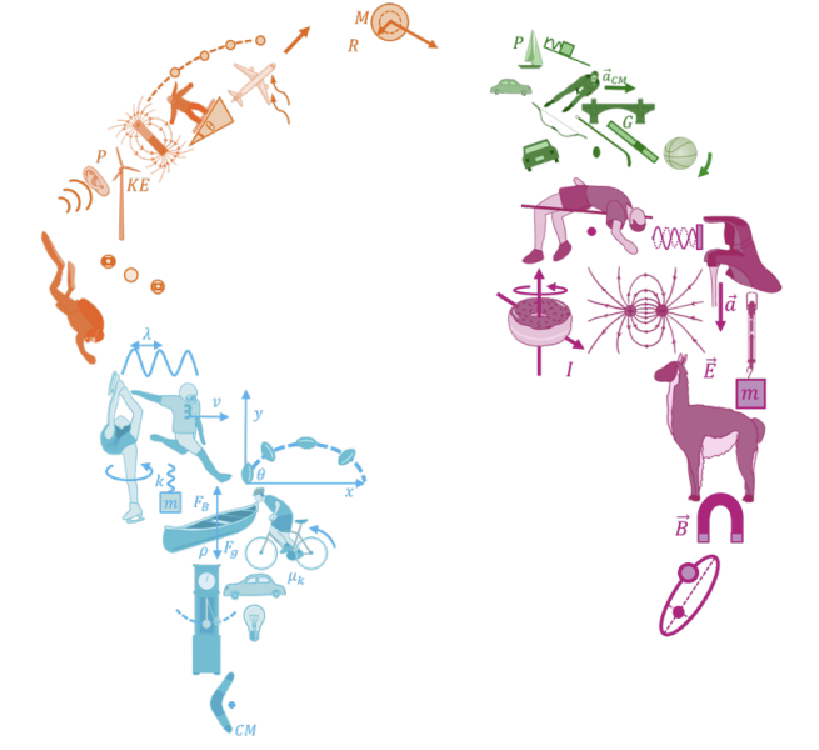
\includegraphics[width=4cm]{figures/BMDW/logo}
\end{textblock*}

\end{frame}

%%%%%%%%%%%%%%%%%%%%%%%%%%%%%%%%%





\twocolframe{Outline}
{\tableofcontents[sections=19, subsectionstyle=show/show]\thispagestyle{empty}}
{\tableofcontents[sections=20-21, subsectionstyle=show/show]}






%%%%%%%%%%%%%%%%%%%%%%%%%%%%%%%%%%%%%%%

\section{Conservative Forces}
\label{sec:conservativeforces}
\title{Conservative Forces}
\institute{Conservation, Potential and Potential Uses}
\author{\insertsubsection}


%%%%%%%%%%%%%%%%%%%%%%%%%
\begin{frame}
\titlepage
\thispagestyle{empty}
\end{frame}

%%%%%%%%%%%%%%%%%%%%%%%%




\subsection{Work Recap}
\label{subsec:workrecap}
\twocolframesf{Recall: Work}
{
\begin{align*}
W=\int_A^B \vec F(\vec r) \cdot d\vec l
\end{align*}
\begin{itemize}
\item Force can change magnitude and direction based on position.
\item Need to define work as a ``path integral'', as it depends on the path taken.
\item In general, this integral can be difficult to evaluate.
\end{itemize}
}
{
\vspace{-1cm}
\begin{center}
\begin{tikzpicture}[%
%https://tex.stackexchange.com/questions/25928/how-to-draw-tangent-line-of-an-arbitrary-point-on-a-path-in-tikz
        tangent/.style={
        decoration={
            markings,% switch on markings
            mark=
                at position ####1
                with
                {
                    \coordinate (tangent point-\pgfkeysvalueof{/pgf/decoration/mark info/sequence number}) at (0pt,0pt);
                    \coordinate (tangent unit vector-\pgfkeysvalueof{/pgf/decoration/mark info/sequence number}) at (1,0pt);
                    \coordinate (tangent orthogonal unit vector-\pgfkeysvalueof{/pgf/decoration/mark info/sequence number}) at (0pt,1);
                }
        },
        postaction=decorate
    },
    use tangent/.style={
        shift=(tangent point-####1),
        x=(tangent unit vector-####1),
        y=(tangent orthogonal unit vector-####1)
    },
    use tangent/.default=1
    ]
\tikzmath{
}

\scalebox{0.8}{

 \coordinate (P1) at (0.2,0.5);
 \coordinate (P2) at (1.75,2); %used to make the path squiggly
 \coordinate (P3) at (3.75,2.5);
 \coordinate (P3x) at ($(0,0)!(P3)!(1,0)$);
 \coordinate (P1P3) at ($(P3)!(P1)!(P3x)$);
 
 \draw[-latex, line width=1.5pt] (0,0) -- (4.5,0) node[below]{$x$}; 
 \draw[-latex, line width=1.5pt] (0,0) -- (0,3) node[left]{$y$}; 
 
 \fill (P1) circle(2pt) node[above]{$A$};;
 \fill (P3) circle(2pt) node[above]{$B$};;
 
  
 %The path with tangent coordinates calculated
 \draw[tangent=0.25,tangent=0.45,tangent=0.65, tangent=0.85,  line width=1pt] (P1) to [out=10,in=190] (P2) to [out=10,in=260] (P3);
 
 \draw [myred, -latex, line width=1.5, use tangent=2] (-0.25,0) -- (0.25,0) node[above]{$d\vec l$};
 %\draw [ -latex, line width=1.5, use tangent=2] (0,0) -- +(-60:1) node[right]{$\vec F(\vec r)$}; 
 \draw [ -latex, line width=1.5, use tangent=1] (0,0) -- +(-80:0.75) node[below]{$\vec F(\vec r)$}; 
 %\draw [ -latex, line width=1.5, use tangent=3] (0,0) -- +(60:1.25) node[above]{$\vec F(\vec r)$}; 
 
 \begin{scope}[shift={(0,-3.5)}]
 
 \coordinate (A) at (0.75,0.5);
 \coordinate (B) at (3.75,2.5);
 
 
 \draw[-latex, line width=1.5pt] (0,0) -- (4.5,0) node[below]{$x$}; 
 \draw[-latex, line width=1.5pt] (0,0) -- (0,3) node[left]{$y$}; 

 \fill (A) circle(2pt) node[right]{$A(x_A,y_A)$};
 \fill (B) circle(2pt) node[above]{$B(x_B,y_B)$};
 
 \draw[dashed, line width=1.5] (A)--(B) node[midway,right=5pt]{path 1};
 
 \draw[-latex, color=myred, line width=1.5pt] (A)-- +(0,2.0)node[midway,left]{$\vec d_1$} node[above]{path 2};
 \draw[latex-, color=myred, line width=1.5pt] (B)-- +(-3,0) node[midway,above]{$\vec d_2$};
 
 \draw[latex-, line width=3] (1,1) -- +(0,1) node[midway, right]{$\vec f_1$};
 \draw[-latex, line width=3] (2.5,2.25) -- +(-1,0) node[midway, below]{$\vec f_2$};
 
 
 \end{scope} 
 
}
\end{tikzpicture}
\captionof*{figure}{\textit{Work is a path integral.}}
\end{center}
}


%%%%%%%%%%%%%%%%%%%%%%%%%%%%%%%%
\twocolframest{Recall: Work-Energy Theorem}
{
\only<1>{
\begin{itemize}
\item The net work done on an object is its change in kinetic energy:
\begin{align*}
W^{net}=\Delta K
\end{align*}
\end{itemize}}
\only<2>{
\begin{exampleblock}{Example: Object falling due to gravity}
The work done by gravity:
\begin{align*}
W^{net}=\vec F_g \cdot \vec d = mgh
\end{align*}
The change in kinetic energy (final - initial)
\begin{align*}
\Delta K = \frac{1}{2}mv^2-0=\frac{1}{2}mv^2
\end{align*}
Work-Energy theorem:
\begin{align*}
W^{net}&=\Delta K\\
mgh &=\frac{1}{2}mv^2\\
\therefore v&=\sqrt{2gh}
\end{align*}
\end{exampleblock}
}
}
{
\only<2>{
\begin{center}
\begin{tikzpicture}
\tikzmath{
\h=3;
}

\scalebox{1}{
\fill (0,0) circle(5pt);
\draw [-latex,line width=2] (0,0) -- +(0,-1) node[left]{$\vec F_g$};
\draw [latex-latex,line width=1] (0.5,0) -- +(0,-\h) node[midway,left]{$h$}; 
\draw [-latex,line width=2] (1,0) -- +(0,-\h) node[midway,right]{$\vec d$}; 
}
\end{tikzpicture}
\captionof*{figure}{\textit{A mass, $m$, falls a distance, $h$, with a corresponding displacement, $\vec d$.}}
\end{center}}

}


%%%%%%%%%%%%%%%%%%%%%%%%%%%%%%%%
\subsection{Conservative vs non-conservatice forces}
\label{subsec:conservativevsnonconservativeforces}
\begin{frame}{Conservative vs non-conservative forces}
\begin{itemize}
\item A non-conservative force is one for which the work done depends on the path taken.
\item A conservative force is one for which the work done does not depend on the path taken:
\begin{itemize}
\item Corollary: The work done by a conservative force along a closed path is zero.
\end{itemize}
\end{itemize}
\end{frame}


%%%%%%%%%%%%%%%%%%%%%%%%%%%%%%%%


%%%%%%%%%%%%%%%%%%%%%%%%%%%%%%%%
\subsubsection{Condition for a force to be conservative}
\label{subsec:conditionforconservativeforce}
\begin{frame}{Condition for a force to be conservative}
\begin{itemize}
\item The work done on a closed path must be zero:
\begin{align*}
W=\textcolor{myred}{\int_A^A}\vec F(\vec r) \cdot d\vec l = \textcolor{myred}{\oint}\vec F(\vec r) \cdot d\vec l = 0
\end{align*}
\item This requires the following conditions on, $\vec F(\vec r)$, (given by Stokes' Theorem, which is way beyond the scope of this course):
\begin{align*}
\frac{\partial F_z}{\partial y}-\frac{\partial F_y}{\partial z}&=0\\
\frac{\partial F_x}{\partial z}-\frac{\partial F_z}{\partial x}&=0\\
\frac{\partial F_y}{\partial x}-\frac{\partial F_x}{\partial y}&=0
\end{align*}
... evaluating these partial derivatives is however not beyond the scope of this course!
\end{itemize}
\end{frame}


%%%%%%%%%%%%%%%%%%%%%%%%%%%%%%%%
\begin{frame}{Example of a conservative force}
\begin{itemize}
\item The force from a spring:
\begin{align*}
\vec F(\vec r)=\vec F(x,y,z)=F_x \hat x+F_y\hat y+F_z\hat z = -kx\hat x+0\hat y+0\hat z
\end{align*}
\item Take one of the terms:
\begin{align*}
\frac{\partial F_x}{\partial z}-\frac{\partial F_z}{\partial x}=\frac{\partial}{\partial z}( -kx)-\frac{\partial}{\partial x}0=0
\end{align*}
\item They are all zero $\rightarrow$ The force from a spring is conservative !
\end{itemize}
\end{frame}


%%%%%%%%%%%%%%%%%%%%%%%%%%%%%%%%
\subsubsection{Work by a conservative force}
\label{subsubsec:workbyaconservativeforce}
\twocolframesf{Work by a conservative force – Potential energy}
{
\begin{itemize}
\item The work done by a conservative force does not depend on the path, only on the end points:
\begin{align*}
W=\int_A^B \vec F(\vec r) \cdot d\vec l
\end{align*}
\item We introduce a \textbf{function of position}, $U(\vec r)$ , such that the \textbf{negative of the work} done by the conservative force can be calculated using that function:
\begin{align*}
-W=-\int_A^B \vec F(\vec r) \cdot d\vec l=U(\vec r_B)-U(\vec r_A)=\Delta U
\end{align*}
\end{itemize}
}
{
\vspace{-1cm}
\begin{center}
\begin{tikzpicture}[%
%https://tex.stackexchange.com/questions/25928/how-to-draw-tangent-line-of-an-arbitrary-point-on-a-path-in-tikz
        tangent/.style={
        decoration={
            markings,% switch on markings
            mark=
                at position ####1
                with
                {
                    \coordinate (tangent point-\pgfkeysvalueof{/pgf/decoration/mark info/sequence number}) at (0pt,0pt);
                    \coordinate (tangent unit vector-\pgfkeysvalueof{/pgf/decoration/mark info/sequence number}) at (1,0pt);
                    \coordinate (tangent orthogonal unit vector-\pgfkeysvalueof{/pgf/decoration/mark info/sequence number}) at (0pt,1);
                }
        },
        postaction=decorate
    },
    use tangent/.style={
        shift=(tangent point-####1),
        x=(tangent unit vector-####1),
        y=(tangent orthogonal unit vector-####1)
    },
    use tangent/.default=1
    ]
\tikzmath{
}

\scalebox{1}{

 \coordinate (P1) at (1,1.5);
 \coordinate (P2) at (1.75,2); %used to make the path squiggly
 \coordinate (P3) at (3.75,3);

 \draw[color=myblue!60,-latex, line width = 1.5] (0,0) -- (P1) node[midway, above=5pt,left=-4pt]{$\vec r_A$};
  \draw[color=myblue!60,-latex, line width = 1.5] (0,0) -- (P3) node[midway, below]{$\vec r_B$};
  
 \draw[-latex, line width=1.5pt] (0,0) -- (4.5,0) node[below]{$x$}; 
 \draw[-latex, line width=1.5pt] (0,0) -- (0,3) node[left]{$y$}; 
 
 \fill (P1) circle(2pt) node[right]{$A$};;
 \fill (P3) circle(2pt) node[right]{$B$};;
 
 \node[above=8pt,left=-5pt] at (P1) {$U(\vec r_A)$};
  \node[above] at (P3) {$U(\vec r_B)$};
  
 %The path with tangent coordinates calculated
 \draw[tangent=0.25,tangent=0.45,tangent=0.65, tangent=0.85,  line width=2pt] (P1) to [out=10,in=190] (P2) to [out=10,in=260] (P3);
 
 \draw [myred, -latex, line width=1.5, use tangent=3] (-0.25,0) -- (0.25,0) node[below]{$d\vec l$};
 \draw [ -latex, line width=1.5, use tangent=2] (0,0) -- +(80:0.75) node[above]{$\vec F(\vec r)$}; 

 
}
\end{tikzpicture}
\captionof*{figure}{\textit{Work done by a conservative force depends only on the end points.}}
\end{center}
$U(\vec r)$ is called the \textbf{potential energy function}. It is associated with a specific conservative force and \textbf{depends only on position}.
}


%%%%%%%%%%%%%%%%%%%%%%%%%%%%%%%%
\subsection{Example: potential energy for a spring}
\label{subsec:potentialenergyspringexample}
\twocolframesf{Example: Potential energy for a spring}
{
\begin{itemize}
\item We want to know the potential energy function for a spring. We start with Work:
\begin{align*}
-W=-\int_A^B\vec F(\vec r) \cdot \textcolor{myred}{d\vec l}=U(\vec r_B) - U(\vec r_A)
\end{align*}
\item<2-> Work from the spring in going from $A$ ($x=-d$) to $B$ ($x=0$):
\begin{align*}
-W=-\int_{-d}^0 -kx\hat x \cdot \textcolor{myred}{dx\hat x}=\int_{-d}^0kxdx=\frac{1}{2}k0^2-\frac{1}{2}kd^2
\end{align*}
\item<3-> Identify:
\begin{align*}
U(x)=\frac{1}{2}kx^2+C
\end{align*}
\end{itemize}
}
{
\begin{center}
\begin{tikzpicture}[scale=1]
\tikzmath{
\L=2.;
\dx=0.75*\L;
\off=0.5;
\h=0.75;
}
\scalebox{1}{

\begin{scope}[shift={(0,-2*\h)}]
\draw[-latex,line width=1.5pt] (-1.5*\L,0) -- (1.25*\L,0) node[below]{$x$};
\draw[line width=1.5pt] (0,-0.1) -- (0,0.1);
\node[below] at (0,0) {$0$};

\fill (-1.5*\L,0) rectangle (-1.4*\L,\h);
\draw[decoration={aspect=0.3, segment length=2.4mm, amplitude=2mm,coil},decorate] (-1.4*\L,\h/2) -- (0,\h/2);
%\draw [latex-latex] (-1.4*\L,\h) -- (0,\h) node[midway,above]{$L_0$};
\fill[color=myblue!60] (0,0) rectangle (\h,\h);
\draw [-latex, line width=2] (-\dx,1.1*\h) -- (0,1.1*\h) node[midway,above]{$\vec d$};
 \node[below] at (-\dx,0) {$-d$};
 \draw[line width=1.5pt] (-\dx,-0.1) -- (-\dx,0.1);
\end{scope}
%%%%%%%%%%   compressed

\draw[-latex,line width=1.5pt] (-1.5*\L,0) -- (1.25*\L,0) node[below]{$x$};
\draw[line width=1.5pt] (0,-0.1) -- (0,0.1);
\node[below] at (0,0) {$0$};

\fill (-1.5*\L,0) rectangle (-1.4*\L,\h);
\draw[decoration={aspect=0.3, segment length=1.1mm, amplitude=2mm,coil},decorate] (-1.4*\L,\h/2) -- (-\dx,\h/2);

\fill[color=myblue!60] (-\dx,0) rectangle (-\dx+\h,\h);
\draw[line width=2, -latex,color=myred] (-\dx,\h/2) -- +(1.3,0) node[right] {$\vec F$};
\draw[dotted,line width=2] (-\dx,0) -- +(0,-2*\h);

}
\end{tikzpicture}
\vspace{-0.2cm}
\captionof*{figure}{\textit{Work done by a spring force,$\vec F(x)=-kx \hat x$ , from $x=-d$ to $x=0$. }}
\end{center}
\only<3>{
\textcolor{myred}{We can only determine potential energy up to a constant, since \textbf{only the difference in $U(x)$ is related to work}. Like an anti-derivative...} 
}
}


%%%%%%%%%%%%%%%%%%%%%%%%%%%%%%%%
\subsection{Work-energy and potential energy}
\label{subsec:workenergyandpotentialenergy}
\begin{frame}{Work-Energy Theorem and potential energy}
\begin{itemize}
\item The net work done can be  split into the sum of work done by conservative and non-conservative forces:
\begin{align*}
W^{net}=W^{NC}+W^{C}=\Delta K
\end{align*}
\item Re-arrange:
\begin{align*}
W^{NC}=\Delta K \textcolor{myred}{-}W^C
\end{align*}
\item Use potential energy for work done by conservative force:
\begin{align*}
W^{NC}=\Delta K \textcolor{myred}{+}\Delta U
\end{align*}
\item<2> This is why we introduced a minus sign when defining change in potential energy as the negative of work done, $\textcolor{myred}{-}W=\Delta U$.
\end{itemize}
\end{frame}


%%%%%%%%%%%%%%%%%%%%%%%%%%%%%%%%
\begin{frame}{Interpretation}
\begin{itemize}
\item The work done by non-conservative forces will change the ``energy'' (potential + kinetic) in the system:
\begin{align*}
W^{NC}=\Delta K +\Delta U=\Delta E
\end{align*}
\item Work done by non-conservative forces can \textit{add or remove} energy from the system:
\begin{itemize}
\item You push on a crate (do positive work), that energy goes into kinetic energy of the crate and/or (say) gravitational potential energy (if you push the crate up an incline).
\item A crate slides down an incline, the (negative) work done by friction removes energy, so the crate will have less kinetic energy than it otherwise would have.

\end{itemize}

\end{itemize}
\end{frame}


%%%%%%%%%%%%%%%%%%%%%%%%%%%%%%%%
\subsection{Force from potentital energy}
\label{subsec:forcefrompotentialenergy}
\begin{frame}{Force from potential energy (e.g. for a spring)}
\begin{itemize}
\item Effectively, the \textbf{potential energy can be found from the anti-derivative} of a force function (if we take the path integral on a path parallel to the direction of the force):
\begin{align*}
-W=-\int_{-d}^0 F(x) dx=\int_{-d}^0 kxdx=\frac{1}{2}k0^2-\frac{1}{2}kd^2=U(0)-U(-d)
\end{align*}
where we easily identified $U(x)=\frac{1}{2}kx^2+C$.
\item The force can then be found from the derivative of the potential energy function:
\begin{align*}
F(x)=-\frac{dU}{dx}=-\frac{d}{dx}\left(\frac{1}{2}kx^2+C\right)=-kx
\end{align*}
The signs matter, be careful!
\end{itemize}
\end{frame}


%%%%%%%%%%%%%%%%%%%%%%%%%%%%%%%%
\begin{frame}{Force from potential energy in 3D}
\begin{itemize}
\item In 3D, the potential energy is a \textbf{scalar function} of space, $U(x,y,z)$. 
\item The force \textbf{vector} is given by the negative of the \textbf{gradient vector} of the potential energy function (which you find with the partial derivatives):
\begin{align*}
\vec F &= -\nabla U(x,y,z)\\
F_x&=-\frac{\partial}{\partial x}U(x,y,z)\\
F_y&=-\frac{\partial}{\partial y}U(x,y,z)\\
F_z&=-\frac{\partial}{\partial z}U(x,y,z)
\end{align*}
\end{itemize}
\end{frame}


%%%%%%%%%%%%%%%%%%%%%%%%%%%%%%%%













%%%%%%%%%%%%%%%%%%%%%%%%%%%%%%%%

\section{Conservation of Energy}
\label{sec:conservationofenergy}
\title{Conservation of Energy}
\institute{Conservation, Potential and Potential Uses}
\author{\insertsubsection}


%%%%%%%%%%%%%%%%%%%%%%%%%
\begin{frame}
\titlepage
\thispagestyle{empty}
\end{frame}

%%%%%%%%%%%%%%%%%%%%%%%%%%%%%%%%














%%%%%%%%%%%%%%%%%%%%%%%%%%%%%%%%
\subsection{Potential energy - recap}
\label{subsec:potentialenergyrecap}
\begin{frame}{Potential energy - recap}
\begin{itemize}
\item Some forces are conservative:
\begin{itemize}
 \item[$\rightarrow$] Can define a potential energy for those forces.
 \item[$\rightarrow$] Potential energy is only defined up to a constant (that you can choose).
\end{itemize}

\item \textbf{Change in potential energy} is equal to the negative of the work done by that force:
\begin{align*}
\Delta U = -W=-\int_A^B \vec F(\vec r)\cdot d \vec l
\end{align*}
\item Can use this in the work-energy theorem:
\begin{align*}
W^{net}&=W^{NC}+W^C=\Delta K\\
\therefore W^{NC}&=\Delta K + \Delta U
\end{align*}
\end{itemize}

\end{frame}


%%%%%%%%%%%%%%%%%%%%%%%%%%%%%%%%


%%%%%%%%%%%%%%%%%%%%%%%%%%%%%%%%
\begin{frame}{Potential energy}
\begin{itemize}
\item Potential energy depends on position (and thus on an arbitrary choice of coordinate system).
\item Only \textbf{changes} in potential energy are meaningful:
\begin{itemize}
\item \textit{Change} in potential energy does not depend on our choice of coordinate system.
\item Net work done is change in kinetic energy.
\item Work done by a conservative force is change in associated potential energy.
\item If you think about potential being the anti-derivative of force, then only difference in anti-derivatives (aka definite integrals) give useful physical information.
\end{itemize}
\item Potential energy increases when you move in the direction opposite of the associated force (think gravity, $mgh$).
\end{itemize}
\end{frame}


%%%%%%%%%%%%%%%%%%%%%%%%%%%%%%%%
\subsection{Coordinate choice}
\label{subsec:coordinatechoice}
\begin{frame}{Changes in energy are independent of choice of coordinates}
Consider a ball falling a total distance, $h$, from $A$ to $B$. Is the change in potential energy positive or negative?

 \begin{columns}
 \column{0.35\textwidth}
 \only<2>{
 \begin{align*}
U(x)&=mgx\\
U_A&=mgx_A\\
U_B&=mgx_B\\
\\
\Delta U &= U_B-U_A\\
&= mgx_B-mgx_A\\
&=mg(x_B-x_A)\\
\therefore \Delta U & = -mgh
\end{align*}
}
 
 \column{0.3\textwidth}


\begin{center}
\begin{tikzpicture}
\tikzmath{
\h=3;
}

\scalebox{1}{
\fill (0,0) circle(3pt) node[above=2pt]{$A$};
\fill (0,-\h) circle(3pt) node[below=2pt]{$B$};
%\draw [-latex,line width=2] (0,0) -- +(0,-1) node[left]{$\vec F_g$};
\draw [latex-latex,line width=1,dashed] (0,0) -- +(0,-\h) node[midway,left]{$h$}; 
\only<2>{
\draw [-latex, line width=1.5] (-1,-1.2*\h) -- +(0,1.4*\h) node[left]{$x$};
\draw [dashed, line width=1] (0,0) -- (-1,0) node[left]{$x_A$} ;
\draw [dashed, line width=1] (0,-\h) -- (-1,-\h) node[left]{$x_B$} ;
}
\only<3>{
\draw [latex-, line width=1.5] (1,-1.2*\h) node[right]{$x'$} -- +(0,1.4*\h) ;
\draw [dashed, line width=1] (0,0) -- (1,0) node[right]{$x'_A$} ;
\draw [dashed, line width=1] (0,-\h) -- (1,-\h) node[right]{$x'_B$} ;
}

}
\end{tikzpicture}
\captionof*{figure}{\textit{A mass, $m$, falls a distance, $h$.}}
\end{center}
\column{0.35\textwidth}
 \only<3>{
\begin{align*}
U(x')&=-mgx'\\
U_A&=-mgx'_A\\
U_B&=-mgx'_B\\
\\
\Delta U &= U_B-U_A\\
&= -mgx'_B- (-mgx'_A)\\
&=-mg(x_B'-x'_A)\\
\therefore \Delta U & = -mgh
\end{align*}
}
 \end{columns}

\end{frame}


%%%%%%%%%%%%%%%%%%%%%%%%%%%%%%%%
\subsection{Mechanical Energy}
\label{subsec:mechanicalenergy}
\begin{frame}{Mechanical energy}
\begin{itemize}
\item We can define the mechanical energy of an object:
\begin{align*}
E=K+U
\end{align*}
\item If the object went from $A$ to $B$:
\begin{align*}
E_A&=K_A+U_A\\
E_B&=K_B+U_B
\end{align*}
\item The change in mechanical energy is:
\begin{align*}
\Delta E&=E_B-E_A=(K_B+U_B)-(K_A+U_A)\\
\therefore \Delta E&=\Delta K + \Delta U
\end{align*}
\item The work done by non-conservative force is thus equal to the change in mechanical energy of the object:
\begin{align*}
W^{NC}=\Delta E = \Delta K +\Delta U
\end{align*}
\end{itemize}

\end{frame}


%%%%%%%%%%%%%%%%%%%%%%%%%%%%%%%%
\begin{frame}{Interpretation – Conservation of energy}
\begin{align*}
W^{NC}=\Delta E = \Delta K +\Delta U
\end{align*}
\begin{itemize}
\item An object can have potential and/or kinetic energy.
\item Non-conservative forces can do work and change that energy:
\begin{itemize}
\item Positive work $\rightarrow$ The energy increases.
\item Negative work $\rightarrow$ The energy decreases.
\item No work $\rightarrow$ The energy is constant.
\end{itemize}
\item We call this ``conservation of (mechanical) energy''.
\item This is the origin of the term ``conservative'' for a force. It corresponds to those forces for which a potential energy can be defined and results in the total energy being conserved.
\end{itemize}

\end{frame}


%%%%%%%%%%%%%%%%%%%%%%%%%%%%%%%%
\subsubsection{Block sliding down an incline}
\label{subsec:blockslidingdownanincline}
\twocolframesf{Conservation of energy}
{

\begin{itemize}
\item We can model friction as doing negative work on the block, thus decreasing the mechanical energy of an object:
\begin{align*}
W^{NC}=\textcolor{myred}{E_B}-\textcolor{blue}{E_A}
\end{align*}
\item<3-> We can think of this as:
\begin{align*}
\textcolor{myred}{E_B}=\textcolor{blue}{E_A}+W^{NC}
\end{align*}
\item<3> The final energy ($\textcolor{myred}{E_B}$) is equal to the initial energy ($\textcolor{blue}{E_A}$) plus(minus) any energy added(removed), $W^{NC}$, to(from) the system by non-conservative forces.
\end{itemize}

}
{
\vspace{-1.5cm}
\begin{center}
\begin{tikzpicture}[scale=1]
\tikzmath{
\L=4;
\h=1.5;
\abox=0.75;
\R=0.5*\abox;
\th=atan(\h/\L);
\d=\R+\L*cos(\th)/2;
}
\scalebox{1.0}{
\coordinate (Pb1) at (0,\h);%coordinates of box
\coordinate (Pb2) at ($(Pb1)+(-\th:\abox)$);
\coordinate (Pb3) at ($(Pb2)+(90-\th:\abox)$);
\coordinate (Pb4) at ($(Pb3)+(180-\th:\abox)$);
\coordinate (Pc) at (-\R,\h+\R);

\draw[-latex,line width=1.5] (0,0) -- (0,2*\h) node[left] {$z$};
\node[left] at (0,0) {$0$};
\node[left] at (0,\h) {$h$};

%plane and angle
\draw[line width=2pt] (0,\h) -- (0,0) -- (\L,0) -- cycle;
\draw (\L-0.75,0) arc(180:180-\th:0.75) node[midway,left]{$\theta$};


%rotated box
\draw[fill=myblue!60, line width=1] (Pb1) -- (Pb2) -- (Pb3) -- (Pb4) -- cycle ;
\node[color=blue] at ($(Pb3)+(-\abox/2,\abox/2)$) {$A$};
\node at ($(Pb1)+(45-\th:\abox/1.4)$) {$m$};

%box on the ground:
\draw[fill=myblue!40, dashed, line width=1] (1.0*\L,0) -- (1.0*\L+\abox,0) -- (1.0*\L+\abox,\abox) -- (1.0*\L,\abox) -- cycle;
\node[above,color=myred] at (1.0*\L+0.5*\abox,\abox) {$B$};

}
\end{tikzpicture}
\captionof*{figure}{\textit{A block slides down an incline with friction.}}
\end{center}
\scriptsize
\only<2->{
\begin{align*}
U(z)&=mgz\\
\textcolor{blue}{E_A=mgh} \;\;&\text{and}\;\; \textcolor{myred}{E_B=\frac{1}{2}mv^2}\\
W^{NC}&=-f_k\frac{h}{\sin\theta}\\
\therefore -f_k\frac{h}{\sin\theta} &= \textcolor{myred}{\frac{1}{2}mv^2} - \textcolor{blue}{mgh}\\
\only<3>{
\textcolor{myred}{\frac{1}{2}mv^2} &=\textcolor{blue}{mgh}-f_k\frac{h}{\sin\theta}
}
\end{align*}
}
}


%%%%%%%%%%%%%%%%%%%%%%%%%%%%%%%%
\twocolframesf{Conservation of energy}
{

\begin{itemize}
\item We can think of friction as increasing the ``thermal energy'' of the block (it heats up), $Q$, and include an additional type of energy.
\item In general we can think of $W^{NC}$ as some external agent injecting or removing energy, it doesn't have to be mechanical work and we can always account for it in terms of an energy.
\item If we include thermal energy in the system to model friction:
\begin{itemize}
\item All remaining forces are conservative.
\item Energy is always conserved.
\item We should include the incline into our ``system'' since it will share the heat with the block.
\end{itemize}
\end{itemize}

}
{
\vspace{-1.5cm}
\begin{center}
\begin{tikzpicture}[scale=1]
\tikzmath{
\L=4;
\h=1.5;
\abox=0.75;
\R=0.5*\abox;
\th=atan(\h/\L);
\d=\R+\L*cos(\th)/2;
}
\scalebox{1.0}{
\coordinate (Pb1) at (0,\h);%coordinates of box
\coordinate (Pb2) at ($(Pb1)+(-\th:\abox)$);
\coordinate (Pb3) at ($(Pb2)+(90-\th:\abox)$);
\coordinate (Pb4) at ($(Pb3)+(180-\th:\abox)$);
\coordinate (Pc) at (-\R,\h+\R);

\draw[-latex,line width=1.5] (0,0) -- (0,2*\h) node[left] {$z$};
\node[left] at (0,0) {$0$};
\node[left] at (0,\h) {$h$};

%plane and angle
\draw[line width=2pt] (0,\h) -- (0,0) -- (\L,0) -- cycle;
\draw (\L-0.75,0) arc(180:180-\th:0.75) node[midway,left]{$\theta$};


%rotated box
\draw[fill=myblue!60, line width=1] (Pb1) -- (Pb2) -- (Pb3) -- (Pb4) -- cycle ;
\node[color=blue] at ($(Pb3)+(-\abox/2,\abox/2)$) {$A$};
\node at ($(Pb1)+(45-\th:\abox/1.4)$) {$m$};

%box on the ground:
\draw[fill=myblue!40, dashed, line width=1] (1.0*\L,0) -- (1.0*\L+\abox,0) -- (1.0*\L+\abox,\abox) -- (1.0*\L,\abox) -- cycle;
\node[above,color=myred] at (1.0*\L+0.5*\abox,\abox) {$B$};

}
\end{tikzpicture}
\captionof*{figure}{\textit{A block slides down an incline with friction.}}
\end{center}
\scriptsize

\begin{align*}
\textcolor{myred}{Q_B}&=\textcolor{myred}{f_k\frac{h}{\sin\theta}}\\
\textcolor{blue}{E_A}&=\textcolor{blue}{mgh} \\
\textcolor{myred}{E_B}&=\textcolor{myred}{\frac{1}{2}mv^2+Q_B} \\
W^{NC}=0 \;\;&\rightarrow E_B=E_A\\
\therefore \textcolor{myred}{\frac{1}{2}mv^2+f_k\frac{h}{\sin\theta}} &=\textcolor{blue}{mgh}
\end{align*}

}

%%%%%%%%%%%%%%%%%%%%%%%%%%%%%%%%


%%%%%%%%%%%%%%%%%%%%%%%%%%%%%%%%










%%%%%%%%%%%%%%%%%%%%%%%%%%%%%%%

\section{Modelling Potential}
\label{sec:modelingpotential}
\title{Modeling Potential}
\institute{Conservation, Potential and Potential Uses}
\author{\insertsubsection}


%%%%%%%%%%%%%%%%%%%%%%%%%
\begin{frame}
\titlepage
\thispagestyle{empty}
\end{frame}

%%%%%%%%%%%%%%%%%%%%%%%%%%%%%%%%













%%%%%%%%%%%%%%%%%%%%%%%%%%%%%%%%
\subsection{Conservation of mechanical energy}
\label{subsec:conservationofmechanicalenergy}
\begin{frame}{Conservation of mechanical energy}
\begin{itemize}
\item When there is no net work being done by non-conservative forces, the mechanical energy is constant:
\begin{align*}
E&=\text{const.}=E_A=A_B\\
\Delta E&= 0 =\Delta U + \Delta K
\end{align*}
\item Potential and Kinetic energy ``trade off'' with each other:
\begin{align*}
\Delta K = -\Delta U
\end{align*}
\item If the potential energy increases, the kinetic energy must decrease by the same amount, and vice versa, \textit{just like the pendulum}.
\end{itemize}
\end{frame}


%%%%%%%%%%%%%%%%%%%%%%%%%%%%%%%%
\subsection{Example: marble on a track}
\label{subsec:marbleonatrackexample}
\twocolframesf{Example: marble on a track}
{
\begin{itemize}
\item If I place a marble on a track, it will move under the influence of gravity.
\item If I place it higher, it will have more initial energy, $E$.
\item The height at which I place it is a measure of its total energy, $E$ (it's all potential energy when I place the marble at rest).
\item As the marble rolls along the track, it will trade off kinetic and potential energy.
\end{itemize}
}
{
\begin{center}
\begin{tikzpicture}
\tikzmath{
\L=4;
}

\scalebox{1}{

\draw[line width=1.5,-latex] (0,0) -- (1.25*\L,0) node[below] {$x$};
\draw[line width=1.5,-latex] (0,0) -- (0,\L) node[left] {$y$};

\draw[line width = 2]  (0.05*\L,0.75*\L) to [out=0,in=100] (0.4*\L,0.3*\L)  to [out=-80,in=225] (0.55*\L,0.2*\L) to [out=45,in=180] (0.8*\L,0.5*\L) to [out=0,in=160] (1.1*\L,0.1*\L) to [out=-20,in=180] (1.2*\L,0.05*\L);

\fill[myblue!60] ($(0.4*\L,0.3*\L)+(0.025*\L,0.1*\L)$) circle(5pt);

}

\end{tikzpicture}
\captionof*{figure}{\textit{A marble on a track in the vertical-horizontal plane.}}
\end{center}

}




%%%%%%%%%%%%%%%%%%%%%%%%%%%%%%%%
\twocolframesf{Example: marble on a track}
{
\begin{itemize}
\item The track \textbf{is} the gravitational potential energy as a function of horizontal position:
\begin{align*}
U(x)=mgy(x)\propto y(x)
\end{align*}
\item The initial ``height'' of the marble is the energy of the marble.
\item A potential energy function is like a track!
\item The energy of the marble is constant:
\begin{align*}
E&=U(x)+K\\
K&=E-U(x)
\end{align*}
\end{itemize}
}
{
\begin{center}
\begin{tikzpicture}
\tikzmath{
\L=4;
}

\scalebox{1}{

\draw[line width=1.5,-latex] (0,0) -- (1.25*\L,0) node[below] {$x$};
\draw[line width=1.5,-latex] (0,0) -- (0,\L) node[left] {\textcolor{myred}{$U(x)$}};

\draw[line width = 2]  (0.05*\L,0.75*\L) to [out=0,in=100] (0.4*\L,0.3*\L)  to [out=-80,in=225] (0.55*\L,0.2*\L) to [out=45,in=180] (0.8*\L,0.5*\L) to [out=0,in=160] (1.1*\L,0.1*\L) to [out=-20,in=180] (1.2*\L,0.05*\L);

\draw[dashed] ($(0,0.3*\L)+(0,0.1*\L)$) node[left]{$E$} -- ($(0.4*\L,0.3*\L)+(0.025*\L,0.1*\L)$);
\fill[myblue!60] ($(0.4*\L,0.3*\L)+(0.025*\L,0.1*\L)$) circle(5pt);

}

\end{tikzpicture}
\captionof*{figure}{\textit{In 1D, the potential energy function can be thought of as a track for a marble.}}
\end{center}

}


%%%%%%%%%%%%%%%%%%%%%%%%%%%%%%%%
\subsection{Potential energy for a spring}
\label{subsec:potentialenergyforaspring}
\begin{frame}{Potential energy for a spring}
We can interpret any potential energy function as if it were a track upon which we put a marble.
\begin{align*}
U(x)=\frac{1}{2}kx^2
\end{align*}

\begin{columns}[T]
 \column{0.5\textwidth}
 \begin{tikzpicture}[scale=1]
\tikzmath{
\L=2.;
\dx=0.75*\L;
\off=0.5;
\h=1;
}
\scalebox{0.75}{


\draw[-latex,line width=1.5pt] (-1.5*\L,0) -- (1.5*\L,0) node[below]{$x$};
\draw[line width=1.5pt] (0,-0.1) -- (0,0.1);
\node[below] at (0,0) {$0$};

\fill (-1.5*\L,0) rectangle (-1.4*\L,\h);
\draw[decoration={aspect=0.3, segment length=2.8mm, amplitude=3mm,coil},decorate] (-1.4*\L,\h/2) -- (0,\h/2);
\draw [latex-latex] (-1.4*\L,\h) -- (0,\h) node[midway,above]{$L_0$};
\fill[black!50] (0,0) rectangle (\h,\h);

%%%%%%%%%%  top compressed
\begin{scope}[shift={(0,2*\h)}]
\draw[-latex,line width=1.5pt] (-1.5*\L,0) -- (1.5*\L,0) node[below]{$x$};
\draw[line width=1.5pt] (0,-0.1) -- (0,0.1);
\node[below] at (0,0) {$0$};

\fill (-1.5*\L,0) rectangle (-1.4*\L,\h);
\draw[decoration={aspect=0.3, segment length=2mm, amplitude=3mm,coil},decorate] (-1.4*\L,\h/2) -- (-\dx,\h/2);
\fill[black!50] (-\dx,0) rectangle (-\dx+\h,\h);
\draw[line width=2, -latex, color=myred] (-\dx,\h/2) -- +(1.3,0) node[right] {$\vec F$};

\end{scope}
%%%%%%%%%% bottom extended
\begin{scope}[shift={(0,-2*\h)}]
\draw[-latex,line width=1.5pt] (-1.5*\L,0) -- (1.5*\L,0) node[below]{$x$};
\node[below] at (-\dx,0){$-D$};
\draw[line width =1.5pt] (-\dx,0.1) -- +(0,-0.2);
\node[below] at (\dx,0){$+D$};
\draw[line width =1.5pt] (\dx,0.1) -- +(0,-0.2);
\draw[line width=1.5pt] (0,-0.1) -- (0,0.1);
\node[below] at (0,0) {$0$};

\fill (-1.5*\L,0) rectangle (-1.4*\L,\h);
\draw[decoration={aspect=0.3, segment length=3.5mm, amplitude=3mm,coil},decorate] (-1.4*\L,\h/2) -- (\dx,\h/2);
\fill[black!50] (\dx,0) rectangle (\dx+\h,\h);
\draw[line width=2, -latex, color=myred] (\dx,\h/2) -- +(-1.3,0) node[midway,below=-2pt] {$\vec F$};
\end{scope}

}
\end{tikzpicture}
 
 
 \column{0.5\textwidth}
 \vspace{-1.2cm}
 \begin{tikzpicture}
 \scalebox{0.75}{
 \begin{axis}[domain = -3:3, ymin=0,legend pos=north east,
              grid, xtick = {-2, 0, 2}, xticklabels = {$-D$, 0, $+D$}, ytick = {0, 8, 16}, yticklabels = {0, $E$, $2E$}]
  \addplot[smooth,color=blue,line width=2] {2*x^2};
  \addplot[smooth,color=myred,line width=2] {8};
  \addplot[smooth,dashed,line width=2] {8-2*x^2};
  \addlegendentry{$U(x)$}
  \addlegendentry{$E$}
  \addlegendentry{$K$}
  
  \fill[coordinate] (axis cs:-2,8) circle(3pt);
  \fill[coordinate] (axis cs:2,8) circle(3pt);
  
  \node (label) at (axis cs:0,12)  {Turning points};
  \draw[-latex,line width=1.5pt] (label.south west) -- (axis cs:-2,8);
  \draw[-latex,line width=1.5pt] (label.south east) -- (axis cs:2,8);
 \end{axis}

 }
 \end{tikzpicture}
 
 \end{columns}
\end{frame}


%%%%%%%%%%%%%%%%%%%%%%%%%%%%%%%%


%%%%%%%%%%%%%%%%%%%%%%%%%%%%%%%%
\subsection{How to model with energy}
\label{subsec:howtomodelwithenergy}
\begin{frame}{Modeling with energy (how to)}
\begin{itemize}
\item The most important step is \sout{identifying the forces} identifying the potential energies and sources of non-conservative work.
\item Compare energy at some point (time) A and some other point (time) B; the difference in mechanical energies is the work done by non-conservative forces:
\begin{align*}
E_A&=K_A+U_{1A}+U_{2A}+\dots\\
E_B&=K_B+U_{1B}+U_{2B}+\dots\\
\rightarrow W^{NC}&=E_B-E_A
\end{align*}
\end{itemize}

\end{frame}


%%%%%%%%%%%%%%%%%%%%%%%%%%%%%%%%
\subsection{Intro to The Lagrangian}
\label{subsec:introtothelagrangian}
\begin{frame}{The Lagrangian: A completely different approach}
\begin{itemize}
\item You won’t be tested on your knowledge of this, however...
\item It is presented to you as a different way to build models:
\begin{itemize}
\item We give you a prescription and tell you that if you follow those rules, you will develop a model that describes the world.
\item You should be open to that process (following rules, not understanding the rules – nobody can seriously claim to fully understand them).
\end{itemize}

\item The Lagrangian method is very powerful, carries into Quantum Mechanics, and is mathematically very aesthetic. It almost feels as if there is an underlying beauty to it all...
\end{itemize}
\end{frame}


%%%%%%%%%%%%%%%%%%%%%%%%%%%%%%%%
\subsubsection{Structure}
\label{subsubsec:structurelagrangian}
\twocolframe{The prescription}
{
\begin{enumerate}
\item Build the Lagrangian:
\begin{align*}
L=K-U
\end{align*}
\item Apply the Euler-Lagrange equation:
\begin{align*}
\frac{d}{dt}\left( \frac{\partial L}{\partial v_x} \right) - \frac{\partial L}{\partial x} =0
\end{align*}
\end{enumerate}
This gives the equations of motion (e.g. the acceleration).\\
You get one such equation per coordinate (e.g. replace $(x,v_x)$ with $(y, v_y)$ if these also appear in $L$).
}
{
\only<2>{
For a particle falling with gravity ($x$ positive upwards):
\begin{align*}
L&=\frac{1}{2}mv^2-mgx\\
\frac{d}{dt}\left( \frac{\partial L}{\partial v_x} \right) &=\frac{d}{dt}\left(mv \right) = ma\\
\frac{\partial L}{\partial x} &= -mg\\
\therefore ma + mg&=0\\
a&=-g
\end{align*}
As expected, the acceleration is $-g$, since $x$ is positive upwards.

 }

}


%%%%%%%%%%%%%%%%%%%%%%%%%%%%%%%%
\subsubsection{Lagrangian for a pendulum}
\label{subsubsec:lagrangianforapendulum}
\twocolframesf{Lagrangian for a pendulum}
{
For a pendulum, we use the angle $\theta$ as the coordinate to describe position. The speed is given by $v=\omega L$, where $\omega=\frac{d\theta}{dt}$:
\begin{align*}
K&=\frac{1}{2}mv^2=\frac{1}{2}mL^2\omega^2\\
U&=mgh=mgL(1-\cos\theta)\\
\therefore L&=K-U=\frac{1}{2}mL^2\omega^2-mgL(1-\cos\theta)
\end{align*}
The Euler-Lagrange equation is:
\begin{align*}
\frac{d}{dt}\left( \frac{\partial L}{\partial \omega} \right) - \frac{\partial L}{\partial \theta} =0
\end{align*} 
}
{
\vspace{-0.75cm}
\begin{center}
\begin{tikzpicture}[scale=1]
\tikzmath{
\L=3.;
\R=0.3;
\th=40;
\vg=1;
\Ly=\L*cos(\th);
}
\scalebox{1.0}{
%pendulum

\draw[line width = 1.5pt] (0,0) -- (270-\th:\L) node[midway,above]{$L$};
\fill[color=myblue!60] (270-\th:\L) circle(\R); 

\draw[dotted, line width = 1.5pt] (0,0) -- (270:\L);
\draw[dotted, line width = 1.5pt] (270-\th:\L) arc (270-\th:270:\L);
\draw (270-\th:0.75) arc (270-\th:270:0.75) node[midway,below]{$\theta$};
\draw[dotted, line width = 1.5pt] (270-\th:\L) -- (0,-\Ly);
\draw[latex-latex] (0.2,-\L) -- (0.2,-\Ly) node[midway,right]{$h=L(1-\cos\theta)$};
}
\end{tikzpicture}
\end{center}
\only<2>{
\begin{align*}
\frac{d}{dt}\left( \frac{\partial L}{\partial \omega} \right) = \frac{d}{dt}\left( mL^2\omega \right)&=mL^2\alpha\\
\frac{\partial L}{\partial \theta} &=-mgL\sin\theta\\
\therefore mL^2\alpha + mgL\sin\theta&=0\\
\alpha &=\frac{g}{L}\sin\theta
\end{align*}
}
}


%%%%%%%%%%%%%%%%%%%%%%%%%%%%%%%%
\subsubsection{Noether's Theorem}
\label{subsubsec:noethertheorem}
\twocolframesf{Emmy Noether's theorem}
{
\begin{itemize}
\item If the Lagrangian is ``invariant to some symmetry'', then something is conserved.
\item This ties the idea of a conserved quantity to some symmetry in the laws of nature.
\item For example, if the Lagrangian does not change with time, then energy is conserved.
\item We now see conservation laws as the result of symmetries in the laws of physics.
\item Momentum, charge, energy are conserved because the laws of physics are invariant to different ``symmetries''. 
\end{itemize}
}
{\vspace{-0.5cm}
\capfig{0.7}{figures/PotentialECons/noether}{Emmy Noether. (2025, August 12). Wikipedia, the free encyclopedia. Retrieved August 25, 2025, from https://en.wikipedia.org/wiki/Emmy\_Noether}
}  
  

%%%%%%%%%%%%%%%%%%%%%%%%%%%%%%%%
\subsection{The Standard Model of particle physics}
\label{subsec:thestandardmodelofparticlephysics}
\twocolframesf{The Standard Model of particle physics}
{
\begin{itemize}
\item The Standard Model of Particle physics describes the three forces (weak, strong, e/m) of nature that are not gravity. It’s just a Lagrangian.
\item Each term represents some interaction between particles.
\item Only certain functional forms are allowed in order to preserve symmetries.
\item So far, it appears that every (mathematically) allowable term describes something in nature. That’s pretty cool.
\item People have discovered particles based on the idea that a particular term could be present in the Lagrangian. 
\end{itemize}
}
{
\capfig{1.1}{figures/PotentialECons/LSM}{The Lagrangian for the Standard Model.}
} 

%%%%%%%%%%%%%%%%%%%%%%%%%%%%%%%%




























\title{Gravity}
\subject{Kepler, Newton, Gauss and Einstein}
\subtitle{Building Models to Describe our World}




%%%%%%%%%%%%%%%%%%%%%%%%%
%%%%%% Title slide %%%%%%
%%%%%%%%%%%%%%%%%%%%%%%%%
\chaptertitle{Gravity}
\begin{frame}
\label{chap:gravity}
\titlepage
\thispagestyle{empty}

\begin{textblock*}{5cm}(11cm,4cm)
    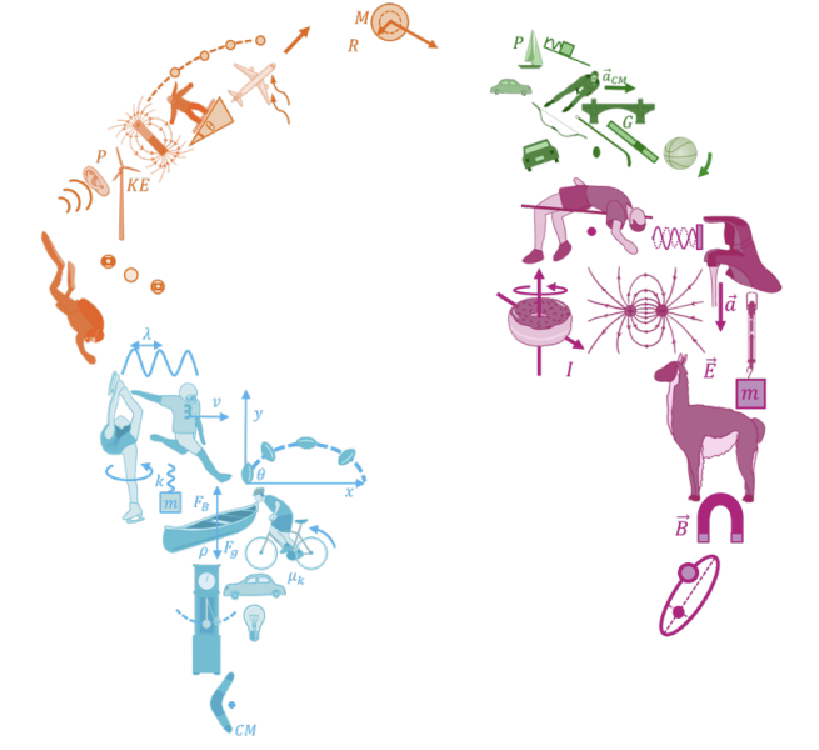
\includegraphics[width=4cm]{figures/BMDW/logo}
\end{textblock*}

\end{frame}

%%%%%%%%%%%%%%





\twocolframe{Outline}
{\tableofcontents[sections=22, subsectionstyle=show/show]\thispagestyle{empty}}
{\tableofcontents[sections=23-24, subsectionstyle=show/show]}





%%%%%%%%%%%%%%%%%%%%%

\section{Keplerian and Newtonian Gravity}
\label{sec:keplernnewtongravity}
\title{Keplerian and Newtonian Gravity}


%%%%%%%%%%%%%%%%%%%%%%%%%
\begin{frame}
\titlepage
\thispagestyle{empty}
\end{frame}

%%%%%%%%%%%%%%%%%%%%%%





\subsection{Kepler's laws}
\label{subsec:keplerslaws}
\begin{frame}{Kepler's Laws}
\begin{enumerate}
\item The path of a planet around the Sun is described by an ellipse with the Sun at one of its foci.
\item All planets move in such a way that the area swept by a line connecting the planet and the Sun in a given period of time is constant.
\item The ratio between the orbital periods, $T$, of two planets squared is equal to the ratio of the semi-major axes, $s$, of their orbits cubed:
\begin{align*}
\left( \frac{T_1}{T_2}\right)^2=\left( \frac{s_1}{s_2}\right)^3
\end{align*}
\end{enumerate}

\end{frame}


%%%%%%%%%%%%%%%%%%%%%%%%%%%%%%%%

%%%%%%%%%%%%%%%%%%%%%%%%%%%%%%%%
\subsubsection{First law}
\label{subsubsec:firstlaw}
\twocolframe{Kepler's First Law}
{
\begin{itemize}
\item Orbits of planets are ellipses (but some bodies that are not in bound orbits will have parabolic or hyperbolic orbits).
\item Ellipses are characterized by the location of two foci and one dimension (e.g. semi-major/minor axis, eccentricity).
\end{itemize}
\begin{align*}
\frac{x^2}{s^2}+\frac{y^2}{b^2}&=1\\
e&=\sqrt{s^2-b^2}\quad(s\geq b)
\end{align*}
}
{
\vspace{-1cm}
\begin{center}
\begin{tikzpicture}
\tikzmath{
\a=2.5;
\b=1.25;
\c=sqrt(\a*\a-\b*\b);
\xe=\a/2;
\ye=\b/2*sqrt(3);
\ae=0.5*\a;
\be=0.7*\b;
\ce=sqrt(\ae*\ae-\be*\be);
\xm=\xe+\ce+\ae/2;
\ym=\ye+\be/2*sqrt(3);
}

\scalebox{1}{
\draw (0,0) ellipse ({\a} and \b);

\draw[latex-latex, line width=1,color=myred] (0,0) -- +(0,\b) node[midway,right]{\scriptsize semi-minor axis, $b$};
\draw[latex-latex, line width=1,color=myred] (0,0) -- +(-\a,0) node[midway,above]{\scriptsize semi-major axis, $s$};
\draw[latex-latex, line width=1,color=myblue!60] (0,0) -- +(\c,0) node[midway,above]{\scriptsize eccentricity, $e$};
\fill (-\c,0) circle(2pt) node[below right]{\scriptsize Focus};
\fill (\c,0) circle(2pt) node[below left]{\scriptsize Focus};

\begin{scope}[shift={(0,-3.5)}]
\draw (0,0) ellipse ({\a} and \b);
\node at (-\c,0)  {
\includegraphics[scale=0.15]{figures/Gravity/sun}};
\node at (\xe,\ye)  {
\includegraphics[scale=0.1]{figures/Gravity/earth}};
\draw (\xe+\ce,\ye) ellipse ({\ae} and \be);
\node at (\xm,\ym)  {
\includegraphics[scale=0.1]{figures/Gravity/moon}};
\fill (-\a,0) circle(2pt) node[left]{\scriptsize perihelion};
\fill (\a,0) circle(2pt) node[left]{\scriptsize aphelion};
\fill (\xe+\ce-\ae,\ye) circle(2pt) node[left]{\scriptsize perigee};
\fill (\xe+\ce+\ae,\ye) circle(2pt) node[left]{\scriptsize apogee};
\end{scope}

}

\end{tikzpicture}
\captionof*{figure}{\textit{Elliptical orbits and their parameters.}}
\end{center}

}

%%%%%%%%%%%%%%%%%%%%%%%%%%%%%%%%
\subsubsection{Second law}
\label{subsubsec:secondlaw}
\twocolframe{Kepler's Second Law}
{
\begin{itemize}
\item ``Equal areas swept out in equal times'':
\begin{itemize}
\item[$\rightarrow$] Planets move faster near the perihelion.
\item[$\rightarrow$] Bodies in a circular orbit move at constant speed.
\end{itemize}

\end{itemize}
}
{

\begin{center}
\begin{tikzpicture}
\tikzmath{
\a=2.5;
\b=1.5;
\c=sqrt(\a*\a-\b*\b);
\tA=20;
\tB=\tA+20;
\tC=110;
\tD=\tC+40;
\Ax=\a*cos(\tA);
\Ay=\b*sin(\tA);
\Bx=\a*cos(\tB);
\By=\b*sin(\tB);
\Cx=\a*cos(\tC);
\Cy=\b*sin(\tC);
\Dx=\a*cos(\tD);
\Dy=\b*sin(\tD);
\thA=atan(\Ay/\Ax);
\thB=atan(\By/\Bx);
\Ar=1.1*sqrt(\Ax*\Ax+\Ay*\Ay);
\Br=1.1*sqrt(\Bx*\Bx+\By*\By);
\Cr=1.1*sqrt(\Cx*\Cx+\Cy*\Cy);
\Dr=1.1*sqrt(\Dx*\Dx+\Dy*\Dy);
\biga=1.3*\a;
\bigb=1.3*\b;
}

\scalebox{1}{

\coordinate (A) at (\Ax,\Ay);
\coordinate (B) at (\Bx,\By);
\coordinate (C) at (\Cx,\Cy);
\coordinate (D) at (\Dx,\Dy);

\begin{scope}
\clip (0,0) ellipse ({\a} and \b);
\fill[color=myblue!40] (-\c,0) -- (\thA:\Ar) -- (\thB:\Br) --cycle;
\fill[color=myblue!40] (-\c,0) -- (\tC:\Cr) -- (\tD:\Dr) --cycle;
\end{scope}

\draw (0,0) ellipse ({\a} and \b);


\fill (A) circle(2pt) node[above, right]{$A$};
\fill (B) circle(2pt) node[above]{$B$};
\fill (C) circle(2pt) node[above]{$C$};
\fill (D) circle(2pt) node[left]{$D$};

\node at (-\c,0)  {
\includegraphics[scale=0.15]{figures/Gravity/sun}};

\draw [-latex, dashed] (\biga,0) arc(0:180:{\biga} and \bigb) node[midway,above]{\scriptsize motion of planet};



}

\end{tikzpicture}
\captionof*{figure}{\textit{Planets sweep out equal areas in equal amounts of time.}}
\end{center}

}


%%%%%%%%%%%%%%%%%%%%%%%%%%%%%%%%
\subsubsection{Third law}
\label{subsubsec:thirdlaw}
\twocolframe{Kepler's Third Law}
{
\begin{itemize}
\item The ratio between the orbital periods, $T$, of two planets squared is equal to the ratio of the semi-major axes, $s$, of their orbits cubed:
\begin{align*}
\left( \frac{T_1}{T_2}\right)^2=\left( \frac{s_1}{s_2}\right)^3
\end{align*}
\item It's a mouthful... But it just means that:
\begin{align*}
\frac{T^2}{s^3}=\text{constant}
\end{align*}
\end{itemize}

}
{

\begin{center}
\begin{tikzpicture}
\tikzmath{
\a=2.5;
\b=1.25;
\c=sqrt(\a*\a-\b*\b);
\xe=\a/2;
\ye=\b/2*sqrt(3);
\ae=0.5*\a;
\be=0.7*\b;
\ce=sqrt(\ae*\ae-\be*\be);
\xm=\xe+\ce+\ae/2;
\ym=\ye+\be/2*sqrt(3);
}

\scalebox{1}{
\draw (0,0) ellipse ({\a} and \b);

\draw[latex-latex, line width=1,color=myred] (0,0) -- +(0,\b) node[midway,right]{\scriptsize semi-minor axis, $b$};
\draw[latex-latex, line width=1,color=myred] (0,0) -- +(-\a,0) node[midway,above]{\scriptsize semi-major axis, $s$};
\draw[latex-latex, line width=1,color=myblue!60] (0,0) -- +(\c,0) node[midway,above]{\scriptsize eccentricity, $e$};
\fill (-\c,0) circle(2pt) node[below right]{\scriptsize Focus};
\fill (\c,0) circle(2pt) node[below left]{\scriptsize Focus};

}

\end{tikzpicture}
\captionof*{figure}{\textit{Kepler's Third Law relates to the semi-major axis.}}
\end{center}
\textit{That constant depends on the mass of the body that the planets orbit (e.g. the Sun). Thus, by measuring $T$ and $s$, you can determine the mass of the Sun!}
}


%%%%%%%%%%%%%%%%%%%%%%%%%%%%%%%%
\subsection{Newton's theory of gravity}
\label{subsec:newtonstheoryofgravity}
\begin{frame}{Newton's Universal Theory of Gravity (magnitude)}
\begin{itemize}
\item Two bodies with mass will exert an \textbf{attractive} force on each other that is proportional to the \textbf{product of their masses} and inversely proportional to the \textbf{distance between them squared}:
\begin{align*}
F \propto \frac{M_1M_2}{r^2}
\end{align*}
\item The constant of proportionality is called the gravitational constant, $G$:
\begin{align*}
F =G \frac{M_1M_2}{r^2}
\end{align*}
\end{itemize}
\end{frame}


%%%%%%%%%%%%%%%%%%%%%%%%%%%%%%%%
\subsubsection{The Cavendish experiment}
\label{subsubsec:thecavendishexperiment}
\twocolframesf{The Cavendish experiment}
{
\begin{itemize}
\item Want to measure G.
\item The forces involved are minuscule (less than \num{1e-6} Newtons).
\item Clever use of a ``torsion pendulum'': two masses suspended by a thin fibre.
\item Bring two big masses close to the suspended masses and measure by how much they twist.
\item Very sensitive experiment... 
\end{itemize}
}
{
\capfig{1}{figures/Gravity/cavendish}{Figure from Cavendish's paper showing the torsion pendulum and building it was housed in. The large masses could be rotated from the outside through a system of pulleys. Philosophical Transactions of the Royal Society of London, (part II) \textbf{88} p.469-526 (21 June 1798).}
}


%%%%%%%%%%%%%%%%%%%%%%%%%%%%%%%%


%%%%%%%%%%%%%%%%%%%%%%%%%%%%%%%%
\subsubsection{Magnitude and direction}
\label{subsec:magnitudeanddirection}
\twocolframesf{Newton's Universal Theory of Gravity (magnitude and direction)}
{
The force, $\vec F_{12}$, \textbf{on} mass $M_1$ \textbf{from} $M_2$ can be written as:
\begin{align*}
\vec F_{12} = - G \frac{M_1M_2}{r_{12}^2}\hat r_{12}=-G \frac{M_1M_2}{r_{12}^{\textcolor{myred}{3}}} \textcolor{myred}{\vec r_{12}}
\end{align*}
where:
\begin{align*}
\vec r_{12}=\vec r_1 - \vec r_2\;\;\text{and}\;\; \hat r_{12}=\frac{\vec r_{12}}{r_{12}}
\end{align*}
In general, we use the \textbf{minus sign to indicate that the force is attractive} (we could've used a plus sign and the vector $\vec r_2 -\vec r_1$, but we don't!).
}
{
\begin{center}
\begin{tikzpicture}
\tikzmath{
\L=4;
}
\scalebox{1}{

\coordinate (M1) at (0.2*\L, 0.6*\L);
\coordinate (M2) at (0.8*\L, 0.75*\L);

\draw[-latex,line width=1.5] (0,0) -- (\L,0) node[below]{$x$};
\draw[-latex,line width=1.5] (0,0) -- (0,\L) node[left]{$y$};

\fill (M1) circle (3pt) node[above left]{$M_1$};
\fill (M2) circle (3pt) node[above right]{$M_2$};

\draw[-latex,line width=1] (0,0) -- (M1) node[midway,right] {$\vec r_1$};
\draw[-latex,line width=1] (0,0) -- (M2) node[midway,right] {$\vec r_2$};

\draw[-latex,line width=2, color=myred] ($(M1)+(0,0.3)$) -- ($(M1)!0.4!(M2)+(0,0.3)$) node[above] {$\vec F_{12}$};
\draw[-latex,line width=1.5, color=myblue!60] (M2) -- (M1) node[midway,below] {$\vec r_{12}$};

}

\end{tikzpicture}
\captionof*{figure}{\textit{Vectors in Newton's Universal Theory of Gravity. The force on $M_1$ is in the opposite direction of $\vec r_{12}$.}}
\end{center}
}


%%%%%%%%%%%%%%%%%%%%%%%%%%%%%%%%

%%%%%%%%%%%%%%%%%%%%%%%%%%%%%%%%
\subsubsection{M > > > m}
\label{subsubsec:mmuchgreaterthanm}
\twocolframesf{When one mass is much larger}
{
\begin{itemize}
\item If $M$ is much bigger than $m$, $M$ can be considered as effectively stationary (e.g. the Sun when considering the motion of planets, the Earth when considering the motion of satellites).
\item Makes sense to make $M$ the origin of our coordinate system, so the force on $m$ (at position, $\vec r$ is):
\begin{align*}
\vec F = - G \frac{Mm}{r^2}\hat r= - G \frac{Mm}{r^3}\vec r
\end{align*}
\end{itemize}
}
{
\begin{center}
\begin{tikzpicture}
\tikzmath{
\L=4;
}
\scalebox{1}{

\coordinate (M) at (0,0);
\coordinate (m) at (0.8*\L, 0.75*\L);

\draw[-latex,line width=1.5] (0,0) -- (\L,0) node[below]{$x$};
\draw[-latex,line width=1.5] (0,0) -- (0,\L) node[left]{$y$};

\fill (M) circle (0.5) node[left=15pt]{$M$};
\fill (m) circle (5pt) node[above right]{$m$};

\draw[color=myred,-latex,line width=2] (M) -- (m) node[midway,below] {$\vec r$};

}

\end{tikzpicture}
\captionof*{figure}{\textit{Newton's Universal Theory of Gravity with one mass at the origin.}}
\end{center}
}


%%%%%%%%%%%%%%%%%%%%%%%%%%%%%%%%
\subsection{The constant from Kepler's third law}
\label{subsec:thecnstfromkeplersthirdlaw}
\twocolframe{The constant from Kepler's Third Law}
{
\vspace{-0.25cm}
\begin{itemize}
\item The constant is given by:
\begin{align*}
\frac{T^2}{s^3}=\text{constant}
\end{align*}
\item<2-> Can evaluate this using a circular orbit:
\begin{align*}%
G\frac{Mm}{r^2}=m\frac{v^2}{r}\;\;&\rightarrow\;\; v=\sqrt{\frac{GM}{r}}\\%
v=\frac{2\pi r}{T}\;\;&\rightarrow\;\;T=\frac{2\pi r}{v}=\frac{2\pi r}{\sqrt{\frac{GM}{r}}} %
\end{align*}%
\item<3-> The constant is then given by:
\begin{align*}
\frac{T^2}{r^3}=\frac{4\pi^2 r^2}{r^3\frac{GM}{r}}=\frac{4\pi^2}{GM}
\end{align*}
\end{itemize}

}
{
\vspace{-0.5cm}
\begin{center}
\begin{tikzpicture}
\tikzmath{
\a=2.5;
\b=1.25;
\c=sqrt(\a*\a-\b*\b);
\xe=\a/2;
\ye=\b/2*sqrt(3);
\ae=0.5*\a;
\be=0.7*\b;
\ce=sqrt(\ae*\ae-\be*\be);
\xm=\xe+\ce+\ae/2;
\ym=\ye+\be/2*sqrt(3);
}

\scalebox{1}{
\draw (0,0) ellipse ({\a} and \b);

\draw[latex-latex, line width=1,color=myred] (0,0) -- +(0,\b) node[midway,right]{\scriptsize semi-minor axis, $b$};
\draw[latex-latex, line width=1,color=myred] (0,0) -- +(-\a,0) node[midway,above]{\scriptsize semi-major axis, $s$};
\draw[latex-latex, line width=1,color=myblue!60] (0,0) -- +(\c,0) node[midway,above]{\scriptsize eccentricity, $e$};
\fill (-\c,0) circle(2pt) node[below right]{\scriptsize Focus};
\fill (\c,0) circle(2pt) node[below left]{\scriptsize Focus};


\begin{scope}[shift={(0,-3)}]
\only<2->{
\draw[dashed] (0,0) circle (0.5*\a);

\fill (45:0.5*\a) circle (3pt) node[right=3pt]{$m$};
\fill (0,0) circle (5pt) node[below=5pt]{$M$};
\draw[dashed] (0,0) -- (90:0.5*\a) node[midway,left]{$r$};
\draw [-latex, line width=2,color=myred] (45:0.5*\a) -- +(225:0.3*\a)node[midway,below]{$\vec F_g$};
\node[right] at (0.6*\a,0) {$\sum F=F_g=m\frac{v^2}{r}$};
}
\end{scope}

}

\end{tikzpicture}
\only<2->{
\captionof*{figure}{\textit{For a circular orbit, the semi-major axis is just the radius. The force of gravity is responsible for the radial acceleration.}}
}
\end{center}

}








%%%%%%%%%%%%%%%%%%%%%

\section{The Gravitational Field and Gauss' Law}
\label{sec:gravfieldandgauss}
\title{The Gravitational Field and Gauss' Law}


%%%%%%%%%%%%%%%%%%%%%%%%%
\begin{frame}
\titlepage
\thispagestyle{empty}
\end{frame}

%%%%%%%%%%%%%%%%%%%%%%








%%%%%%%%%%%%%%%%%%%%%%%%
\subsection{Apparent weight}
\label{subsec:apparentweight}
\twocolframesf{Apparent weight}
{
\begin{itemize}
\item Can be defined as \textbf{the net force ($\sum \vec F$) on you minus the force of gravity}.
\item If you stand on a scale, the only 2 forces exerted on you are gravity and the normal force:
\begin{itemize}
\item[$\rightarrow$] The normal force is your apparent weight:
\begin{align*}
\sum \vec F &= \vec F_g+\vec N\\
\vec W &=\sum \vec F - \vec F_g = \vec N
\end{align*}

\item[$\rightarrow$] The scale measures the magnitude of the normal force.
\end{itemize}

\item You feel ``weightless'' when your apparent weight is zero, \textbf{not} when you have no weight.
\end{itemize}
}
{
\begin{center}
\begin{tikzpicture}
\tikzmath{
\L=5;
\w=3;
}

\scalebox{1}{

\draw[line width=1.5] (0,0) rectangle (\w,\L);
\node at (0.25*\w,0.45*\L) {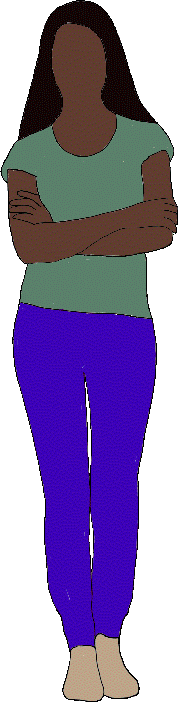
\includegraphics[scale=0.15]{figures/Gravity/woman}} ;
\draw[line width=1.5] (0.1*\w,0.05) rectangle (0.45*\w,0.07*\L);
\node at (0.27*\w,0.035*\L){\scriptsize $W$};
\fill (0.75*\w,0.5*\L) circle (2pt);
\draw[-latex, line width=1.5] (0.75*\w,0.5*\L) -- +(0,1.4) node[midway,right]{$\vec N$};
\draw[-latex, line width=1.5] (0.75*\w,0.5*\L) -- +(0,-1) node[midway,right]{$\vec F_g$};
\draw[-latex, line width=5, color=myred] (1.25*\w,0.4*\L) -- +(0,1.3) node[midway,right]{$\vec a$};
}

\end{tikzpicture}
\captionof*{figure}{\textit{A person on a scale in an elevator accelerating upwards. The scale reads the value of the apparent weight, which is equal to the normal force.}}
\end{center}

}


%%%%%%%%%%%%%%%%%%%%%%%%%%%%%%%%



%%%%%%%%%%%%%%%%%%%%%%%%%%%%%%%%
\twocolframesf{Apparent weight on Earth}
{
\only<1>{
\begin{itemize}
\item At the North Pole, you are not accelerating, so the normal force has the same magnitude as your weight.
\item At the equator, you are accelerating towards the centre of the Earth (uniform circular motion) – the normal force is thus smaller,
\item The effect is small...
\begin{align*}
\vec W &=\sum \vec F - \vec F_g = \vec N\\
\sum F_r&=F_g-N=m\frac{v^2}{R}\\
W&=N=mg=mg-m\frac{v^2}{R}=m\left(g- \frac{v^2}{R} \right)
\end{align*}
\end{itemize}
}
\only<2>{
\begin{itemize}
\item Your apparent weight depends on how fast you rotate about the centre of the Earth:
\begin{align*}
W=m\left(g- \frac{v^2}{R} \right)
\end{align*}
\item If you go just the right speed, your apparent weight will be zero:
\item This is what being ``weightless'' means.
\item If your acceleration is $g$, then you feel weightless. If the only force exerted on you is that from gravity, you feel weightless. 
\end{itemize}
}
}
{
\vspace{-1cm}
\begin{center}
\begin{tikzpicture}
\tikzmath{
\R=2;
}

\scalebox{1}{
\coordinate (P1) at (1.0*\R,0);
\coordinate (P2) at (0,1.0*\R);

\draw[line width=1.5] (0,0) circle (\R);
\draw[dotted, line width=1.5] (\R,0) arc(0:180:{\R} and {\R/4});
\draw[line width=1.5] (\R,0) arc(0:-180:{\R} and {\R/4});
\draw[dashed] (0,0) -- (-\R,0) node[midway,above]{\scriptsize $R$};

\fill (P1) circle (2pt) ;
\draw[-latex,line width=1.5] (P1) -- +(-1,0) node[left]{$\vec F_g$};
\draw[-latex,line width=1.5] (P1) -- +(0.75,0) node[below]{$\vec N$};
\draw[-latex, line width=3] ($(P1)+(1,0.5)$) -- +(-1,0) node[midway,above]{$\vec a$};

\fill (P2) circle (2pt)node[above right]{North Pole};
\draw[-latex,line width=1.5] (P2) -- +(0,-1) node[left]{$\vec F_g$};
\draw[-latex,line width=1.5] (P2) -- +(0,1) node[left]{$\vec N$};


}

\end{tikzpicture}
\captionof*{figure}{\textit{Apparent weight on a rotating Earth. The normal force is smaller at the equator since some of the weight contributes to the centripetal acceleration.}}
\end{center}

}


%%%%%%%%%%%%%%%%%%%%%%%%%%%%%%%%
\twocolframesf{A plumb line}
{

\begin{itemize}
\item We use plumb lines to determine the vertical direction.
\item The mass on the plumb line accelerates with the Earth, so the net force on it is not zero (and the tension is thus not opposite of gravity). The line does not point to the centre of the Earth (except at Pole/Equator).
\item If you cut the line, it’s a little complicated, since the mass does not have an initial speed of zero (as it rotates around the Earth) \url{http://articles.adsabs.harvard.edu/pdf/1897PA......5..186W}
\item The effect is very small for the Earth.
\end{itemize}

}
{

\begin{center}
\begin{tikzpicture}
\tikzmath{
\R=2;
\Rc=\R*cos(30);
}

\scalebox{1}{
\coordinate (P) at (30:1.4*\R);


\draw[line width=1.5] (0,0) circle (\R);
\draw[dotted, line width=1.5] (\R,0) arc(0:180:{\R} and {\R/4});
\draw[line width=1.5] (\R,0) arc(0:-180:{\R} and {\R/4});
\draw[dashed] (0,0) -- (\R,0) node[midway,below]{\scriptsize $R$};

\fill (P) circle (2pt) ;
\draw[-latex,line width=1.5] (P) -- +(210:0.75)node[below right]{$\vec F_g$};
\draw[-latex,line width=1.5] (P) -- +(45:0.5)node[above]{$\vec T$};
\draw[-latex,line width=1, color=myred] (P) -- +(180:0.6)node[midway,above]{$\sum \vec F$};

\draw[dotted, line width=0.5] (30:\R) arc(0:180:{\Rc} and {\Rc/4});
\draw[line width=0.5] (30:\R) arc(0:-180:{\Rc} and {\Rc/4});
\draw[dashed] (30:\R) -- +(-\Rc,0) node[midway,above]{\scriptsize $R\cos\theta$};
\draw[dashed] (0,0) -- (30:\R);
\draw (0.3*\R,0) arc (0:30:0.3*\R) node[midway,right]{\scriptsize $\theta$};
}

\end{tikzpicture}
\captionof*{figure}{\textit{Except at the poles and equator, a plumb line does not point towards the centre of the Earth!}}
\end{center}

}


%%%%%%%%%%%%%%%%%%%%%%%%%%%%%%%%
\subsection{Gravitational field}
\label{subsec:gravitationalfield}
\begin{frame}{Gravitational field}
\begin{itemize}
\item Near the centre of the Earth, we use the force of gravity as:
\begin{align*}
\vec F_g=m\vec g
\end{align*}
\item We call, $\vec g$, the \textbf{gravitational field} of the Earth (rather than the acceleration due to gravity).
\item This has to be the same as the force from Newton's Theory of Gravity:
\begin{align*}
F_g=G\frac{Mm}{R^2}
\end{align*}
\item Thus, in terms of the mass (M) and radius (R) of the Earth, the gravitational field at the surface of the Earth is:
\begin{align*}
g=\frac{F_g}{m}=G\frac{M}{R^2}
\end{align*}
\end{itemize}
\end{frame}


%%%%%%%%%%%%%%%%%%%%%%%%%%%%%%%%
\twocolframesf{Gravitational field, $\vec g$}
{
\begin{itemize}
\item The force on $m$ from $M$:
\begin{align*}
\vec F(\vec r)=-G\frac{Mm}{r^2}\hat r
\end{align*}
\item The force from $M$ \textbf{per unit mass} is called the gravitational field of $M$:
\begin{align*}
\vec g(\vec r)=\frac{\vec F(\vec r)}{m}=-G\frac{M}{r^2}\hat r
\end{align*}
\item The gravitational field is associated with $M$, and makes it easy to calculate the force from $M$ on any mass, $m’$:
\begin{align*}
\vec F'(\vec r)=m'\vec g(\vec r)
\end{align*}
\end{itemize}
}
{
\begin{center}
\begin{tikzpicture}
\scalebox{0.8}{
%Simple way to do a 1/r^2 vector field:
\foreach \x in {-3,-2.5,-2,-1.5,-1,-0.5,0,0.5,1,1.5,2,2.5,3}{%don't need this to be an array...
\foreach \y in {-3,-2.5,-2,-1.5,-1,-0.5,0,0.5,1,1.5,2,2.5,3}{
\tikzmath{
\r=\x*\x+\y*\y+0.001;
\dx=-\x/\r;
\dy=-\y/\r;
}
%ATTENTION: NEED LENGTHTEST to trick it to use float, ifthenelse only works with ints!!!
\ifthenelse{\lengthtest{\r pt> 1.5pt}}{\draw[-latex] (\x,\y) --+(\dx,\dy);}{};
}

}
\node at (0,0){
\includegraphics[scale=0.5]{figures/Gravity/earth}};
}

\end{tikzpicture}
\captionof*{figure}{\textit{Gravitational field vectors around the Earth.}}
\end{center}
}


%%%%%%%%%%%%%%%%%%%%%%%%%%%%%%%%
\subsubsection{Field lines}
\label{subsubsec:fieldlines}
\twocolframesf{Visualizing the gravitational field: field lines}
{
\begin{itemize}
\item If you have a mass M in space, one can think of the gravitational field as existing everywhere in space around M.
\item We can visualize this with \textbf{field lines}.
\item The gravitational field vector is in the \textbf{direction tangent to the field line} and has a \textbf{magnitude proportional to the density of field lines}.
\item Near the surface of the Earth, these are parallel lines downwards.
\end{itemize}
}
{
\vspace{-0.75cm}
\begin{center}
\begin{tikzpicture}
\tikzmath{
\L=3;
}
\scalebox{1}{

\begin{scope}
\clip (-0.6*\L,-0.6*\L) rectangle (0.6*\L,0.6*\L);
\foreach \th in {0,10,...,360}{
\draw (0,0) -- (\th:\L);
\draw[-latex] (\th:0.4*\L) -- +(\th:-0.2);
}
\end{scope}
\node at (0,0){
\includegraphics[scale=0.3]{figures/Gravity/earth}};
\draw[-latex,line width=1.5,color=myred] (40:0.75*\L) -- +(40:-0.15*\L);
\draw[-latex,line width=1.5,color=myred] (-40:0.4*\L) -- +(-40:-0.25*\L);

\begin{scope}[shift={(0,-1.25*\L)}]

\foreach \x in {-0.5, -0.4,...,0.6}{
 \draw (\x*\L,0) -- +(0,0.5*\L);
 \draw[-latex] (\x*\L,0.25*\L) -- +(0,-0.2);
}
\fill[color=brown] (-0.5*\L,0) rectangle (0.5*\L,0.1);
\end{scope}

}

\end{tikzpicture}
\captionof*{figure}{\textit{Gravitational field lines around the Earth. Close to the surface, they are effectively parallel, so the field is essentially constant.}}
\end{center}
}


%%%%%%%%%%%%%%%%%%%%%%%%%%%%%%%%
\subsubsection{Superposition principle}
\label{subsubsec:superpositionprinciple}
\twocolframesf{The Superposition Principle}
{
\begin{itemize}
\item If there are two bodies, say $M_1$ and $M_2$, we can calculate the field from each body separately.
\item The total gravitational field at some point in space is then the sum of the individual gravitational fields.
\item If you calculate the net force on a satellite from both the Earth and Moon, you would add the force vectors. Since the g-field is just the force per unit mass, you can add those together as well.
\item The field from the Moon does not depend on the field from the Earth (superposition).
\end{itemize}
}
{
\begin{center}
\begin{tikzpicture}
\tikzmath{
\xe=-2;%Coordinates of first mass/charge (Earth)
\ye=0;
\xm=2;%Coordinates of first mass/charge (Moon)
\ym=0;
\mee=1;% Mass/charge of first mass (Earth)
\mmm=0.6;% Mass/charge of first mass (Earth)
\dl=0.1;%scale factor to advance along the field line
\n=35;%number of points to find in the line (make as small as possible to reach the point you want!)
}

\scalebox{1}{
%Top field lines (xst is the starting x position of the field line)
\foreach \xst in {-1,-0.8,...,1}{
  \tikzmath{
  \yst=1.5; %all field lines start at yst
  \x=\xst;
  \y=\yst;
  %
  %generate points on the line (keeps finding the next point)
  int \i;
  %note that this also creates \mypairx and \mypairy!
  coordinate \mypair;
  for \i in {1,...,\n}{
    %First mass (earth)
    \re=(\x-\xe)*(\x-\xe)+(\y-\ye)*(\y-\ye)+0.0001;
    \Fex=-\mee*(\x-\xe)/\re;
    \Fey=-\mee*(\y-\ye)/\re;
    %Second mass (moon)
    \rm=(\x-\xm)*(\x-\xm)+(\y-\ym)*(\y-\ym)+0.0001;
    \Fmx=-\mmm*(\x-\xm)/\rm;
    \Fmy=-\mmm*(\y-\ym)/\rm;
    %Total force:
    \Fx=\Fex+\Fmx;
    \Fy=\Fey+\Fmy;
    \Fn=sqrt(\Fx*\Fx+\Fy*\Fy)+0.0001;
    \dx=\Fx/\Fn*\dl;
    \dy=\Fy/\Fn*\dl;
    \x=\x+\dx;
    \y=\y+\dy;
    \mypair{\i}=(\x,\y);
    };
  }
  %Draw that field line
  \foreach \i in {2,...,\n}{
    \tikzmath{
    int \im;
    \im=\i-1;
    }
    \draw (\mypair{\im}) -- (\mypair{\i});
    \ifthenelse{\im =5}{\draw[-latex] (\mypair{\im}) -- (\mypair{\i})}{};%draw arrow on the fifth point
  }

}%end of loop over x

%Bottom field lines
\foreach \xst in {-1,-0.8,...,1}{
  \tikzmath{
  \yst=-1.5;
  \x=\xst;
  \y=\yst;
  %
  %generate points on the line
  int \i;
  %note that this also creates \mypairx and \mypairy!
  coordinate \mypair;
  for \i in {1,...,\n}{
    %First mass (earth)
    \re=(\x-\xe)*(\x-\xe)+(\y-\ye)*(\y-\ye)+0.0001;
    \Fex=-\mee*(\x-\xe)/\re;
    \Fey=-\mee*(\y-\ye)/\re;
    %Second mass (moon)
    \rm=(\x-\xm)*(\x-\xm)+(\y-\ym)*(\y-\ym)+0.0001;
    \Fmx=-\mmm*(\x-\xm)/\rm;
    \Fmy=-\mmm*(\y-\ym)/\rm;
    %Total force:
    \Fx=\Fex+\Fmx;
    \Fy=\Fey+\Fmy;
    \Fn=sqrt(\Fx*\Fx+\Fy*\Fy)+0.0001;
    \dx=\Fx/\Fn*\dl;
    \dy=\Fy/\Fn*\dl;
    \x=\x+\dx;
    \y=\y+\dy;
    \mypair{\i}=(\x,\y);
    };
  }
  %Draw that field line
  \foreach \i in {2,...,\n}{
    \tikzmath{
    int \im;
    \im=\i-1;
    }
    \draw (\mypair{\im}) -- (\mypair{\i});
    \ifthenelse{\im =5}{\draw[-latex] (\mypair{\im}) -- (\mypair{\i})}{};
  }

}%end of loop over x

%Draw the Earth, Moon and example point
\node at (\xe,\ye) {
\includegraphics[scale=0.3]{figures/Gravity/earth}};
\node at (\xm,\ym) {
\includegraphics[scale=0.3]{figures/Gravity/moon}};

%Calculate field vector directions
\tikzmath{
    \xp=1.5;
    \yp=2;
    \fscale=2.5;
    \re=(\xp-\xe)*(\xp-\xe)+(\yp-\ye)*(\yp-\ye)+0.0001;
    \Fex=-\mee*(\xp-\xe)/\re;
    \Fey=-\mee*(\yp-\ye)/\re;
    %Second mass (moon)
    \rm=(\xp-\xm)*(\xp-\xm)+(\yp-\ym)*(\yp-\ym)+0.0001;
    \Fmx=-\mmm*(\xp-\xm)/\rm;
    \Fmy=-\mmm*(\yp-\ym)/\rm;
    %Total force:
    \Fx=\Fex+\Fmx;
    \Fy=\Fey+\Fmy;
    \Fn=sqrt(\Fx*\Fx+\Fy*\Fy)+0.0001;
    \dx=\Fx/\Fn;
    \dy=\Fy/\Fn;
}
\coordinate (P) at (\xp,\yp);
\fill (P) circle(2pt);
\draw[-latex,line width=1] (P) -- +(\fscale*\Fex,\fscale*\Fey) node[above left]{$\vec g_{Earth}$};
\draw[-latex,line width=1] (P) -- +(\fscale*\Fmx,\fscale*\Fmy) node[right]{$\vec g_{Moon}$};
\draw[-latex,line width=1,color=myred] (P) -- +(\fscale*\Fx,\fscale*\Fy) node[below right]{$\vec g_{tot}$};
}

\end{tikzpicture}
\captionof*{figure}{\textit{Gravitational field lines for an Earth-Moon system.}}
\end{center}
}




%%%%%%%%%%%%%%%%%%%%%%%%%%%%%%%%


%%%%%%%%%%%%%%%%%%%%%%%%%%%%%%%%
\subsection{Gauss' law}
\label{subsec:gausslaw}
\begin{frame}{Gauss' Law}
\begin{itemize}
\item Gauss' Law allows us to calculate the magnitude of the gravitational field in situations with high symmetry.
\item \textbf{Newton's Universal Law of Gravity is only valid for point masses} (most masses, like the Earth, are not a point mass) – How would you calculate the gravitational field/force at a location half-way inside the Earth?
\item It is a consequence of Gauss' Law that we can model the Earth as a point mass, with all the mass at the centre of the Earth, if we want to calculate the force of gravity/gravitational field \textbf{outside} of the Earth.	
\end{itemize}

\end{frame}


%%%%%%%%%%%%%%%%%%%%%%%%%%%%%%%%
\subsubsection{Theory}
\label{subsubsec:gausstheory}
\begin{frame}{Gauss' Law - The basic idea}
\begin{center}
\begin{tikzpicture}
\tikzmath{
\L=3;
\R=0.75;
}
\scalebox{1}{

\begin{scope}
\clip (-0.6*\L,-0.6*\L) rectangle (0.6*\L,0.6*\L);
\foreach \th in {0,20,...,360}{
\draw (0,0) -- (\th:\L);
\draw[-latex] (\th:0.4*\L) -- +(\th:-0.2);
}
\end{scope}
\node at (0,0){
\includegraphics[scale=0.3]{figures/Gravity/earth}};

\only<2>{
\shade[ball color=myred, opacity=0.5] (0,0) circle (\R);
\draw[line width=1.5, color=myred, opacity=0.5] (\R,0) arc(0:-180:{\R} and {\R/4});
\node[color=myred] at (50:1.5*\R){$S$};
}

}

\end{tikzpicture}
\captionof*{figure}{\textit{Gravitational field lines around the Earth.\only<2>{ Enclosing the Earth with a gaussian spherical surface, $S$.}}}
\end{center}

\begin{itemize}
\item If you \textbf{enclose} a mass with a surface, $S$, then the number of field lines that cross that surface depends on the mass that you’ve enclosed.
\item<2> Makes sense, if you have a heavier mass, you have a denser field lines, so more of them will enter $S$.
\end{itemize}

\end{frame}


%%%%%%%%%%%%%%%%%%%%%%%%%%%%%%%%
\subsubsection{Formula}
\label{subsubsec:gaussformula}
\begin{frame}{Gauss' Law}
\begin{align*}
\oint \vec g(\vec r) \cdot d\vec A=4\pi G M^{enc}
\end{align*}

\begin{itemize}
\item Two sides to the equation:
\begin{enumerate}
\item Left side: \textbf{flux of the field through the surface}. It is a measure of the number of field lines through the surface.
\item Right-side: amount of \textbf{mass enclosed by the surface} that \textit{we chose}.
\end{enumerate}
\item The flux is a ``surface integral'' over a closed surface. It is the sum of the dot products of the field, $\vec g(\vec r)$ , with a vector, $d\vec A$, that is always normal to the surface.
\item To use Gauss' Law:
\begin{enumerate}
\item Choose a closed surface and figure out how much mass is inside.
\item Figure out how much flux is coming out the surface.
\item Set them equal and determine, say, the gravitational field.
\end{enumerate}
\item Gauss' Law is most useful in situations with a high degree of symmetry (e.g. spherical symmetry).
\end{itemize}
\end{frame}


%%%%%%%%%%%%%%%%%%%%%%%%%%%%%%%%
\subsubsection{Field outside a uniform sphere}
\label{subsubsec:fieldoutsidesphere}
\twocolframesf{Field outside of a uniform sphere of radius, $R$, and mass, $M$}
{
Want the field, $\vec g(\vec r)$, at some distance $r$ from the centre:
\begin{itemize}
\item[1]<2-> Choose a spherical surface ($S$) of radius $r$.
\only<3,4>{
\item[2] Evaluate the flux integral (use symmetry arguments):
\begin{align*}
\oint \vec g(\vec r) \cdot d\vec A=-\oint g(r) dA=-g(r) \oint dA
\end{align*}
\item[$\rightarrow$]<4> Adding together all of the $dA$:
\begin{align*}
\oint dA&=4\pi r^2\\
\therefore \oint \vec g(\vec r) \cdot d\vec A&=-4\pi r^2 g(r)
\end{align*}
}
\only<5>{
\item[2] Evaluate the flux integral: $-4\pi r^2 g(r)$
\item[3] Determine the mass enclosed. In this case, all of $M$ is enclosed:
\begin{align*}
M^{enc}=M
\end{align*}
}
\only<6>{
\item[2] Evaluate the flux integral: $-4\pi r^2 g(r)$
\item[3] Determine the mass enclosed: $M^{enc}=M$
\item[4] Put it all together:
\begin{align*}
\oint \vec g(\vec r) \cdot d\vec A&=4\pi G M^{enc}\\
-4\pi r^2 g(r) &= 4\pi G M \\
\therefore g(r)&=-G\frac{M}{r^2}
\end{align*}
}
\end{itemize}

}
{
\begin{center}
\begin{tikzpicture}
\tikzmath{
\Rm=0.3;
\Rs=1.5;
}
\scalebox{1}{

\shade[ball color=myblue!60] (0,0,0) circle (\Rm);
\only<1>{\node at (-45:2.5*\Rm) {\scriptsize $M,R$};}
\fill (-\Rs,0) circle(2pt);
\draw[dashed,line width=1] (0,0) -- (-\Rs,0) node[midway,above]{$r$};

\only<2->{
\draw[-latex, line width=1] (45:0.775*\Rs) -- +(45:-0.75) node[right=5pt]{$\vec g$};
\shade[ball color=myred, opacity=0.25] (0,0,0) circle (\Rs);
\draw[line width=1.5, color=myred, opacity=0.5] (\Rs,0) arc(0:-180:{\Rs} and {\Rs/4});
\node[color=myred] at (135:1.5*\Rs){$S$};

\fill[color=myred,opacity=0.5, draw=black] (35:0.7*\Rs) -- (37.5:0.85*\Rs) -- (52.5:0.85*\Rs) -- (55:0.7*\Rs) --cycle;
\draw[-latex,color=myred, line width=1] (45:0.775*\Rs) -- +(45:0.75) node[right]{$d\vec A$};
}
}
\end{tikzpicture}
\captionof*{figure}{\textit{Gauss' Law to find field outside of a spherical mass of radius, $R$, and mass, $M$.}}
\end{center}
}


%%%%%%%%%%%%%%%%%%%%%%%%%%%%%%%%
\subsubsection{Field inside a uniform sphere}
\label{subsubsec:fieldinsidesphere}
\twocolframesf{Field \textit{inside} of a uniform sphere of radius, $R$, and mass, $M$}
{
Want the field, $\vec g(\vec r)$, at some distance $r<R$ from the centre:
\begin{itemize}
\item[1]<2-> Choose a spherical surface ($S$) of radius $r$.
\only<3>{
\item[2] Evaluate the flux integral (same as before):
\begin{align*}
\oint \vec g(\vec r) \cdot d\vec A&=-\oint g(r) dA=-g(r) \oint dA\\
&=-4\pi r^2 g(r)
\end{align*}
}
\only<4>{
\item[2] Evaluate the flux integral: $-4\pi r^2 g(r)$
\item[3] Determine the mass enclosed. Use the density, $\rho=\frac{M}{V}$:
\begin{align*}
\rho&=\frac{M}{\frac{4}{3}\pi R^3}\\
M^{enc}&=\rho \frac{4}{3}\pi r^3=\frac{M}{\frac{4}{3}\pi R^3}\frac{4}{3}\pi r^3\\
&=M\frac{r^3}{R^3}
\end{align*}
}
\only<5>{
\item[2] Evaluate the flux integral: $-4\pi r^2 g(r)$
\item[3] Determine the mass enclosed: $M^{enc}=M\frac{r^3}{R^3}$
\item[4] Put it all together:
\begin{align*}
\oint \vec g(\vec r) \cdot d\vec A&=4\pi G M^{enc}\\
-4\pi r^2 g(r) &= 4\pi G M\frac{r^3}{R^3} \\
\therefore g(r)&=-G\frac{M}{R^3}r
\end{align*}
}
\end{itemize}

}
{
\begin{center}
\begin{tikzpicture}
\tikzmath{
\Rm=2;
\Rs=1.25;
}
\scalebox{1}{
\draw[dashed,line width=1] (0,0) -- (-\Rs,0) node[midway,above]{$r$};
\fill (-\Rs,0) circle(2pt);
\only<1>{
\shade[ball color=myblue!60,opacity=0.5] (0,0,0) circle (\Rm);
}
\node at (-45:1.15*\Rm) {\scriptsize $M,R$};



\only<2->{


\draw[-latex, line width=1] (45:0.775*\Rs) -- +(45:-0.75) node[right=5pt]{$\vec g$};
\shade[ball color=myred, opacity=0.25] (0,0,0) circle (\Rs);
\draw[line width=1.5, color=myred, opacity=0.5] (\Rs,0) arc(0:-180:{\Rs} and {\Rs/4});
\node[color=myred] at (135:1.25*\Rs){$S$};

\fill[color=myred,opacity=0.6, draw=black] (35:0.7*\Rs) -- (37.5:0.85*\Rs) -- (52.5:0.85*\Rs) -- (55:0.7*\Rs) --cycle;

\draw[-latex,color=myred, line width=1] (45:0.775*\Rs) -- +(45:0.75) node[right]{$d\vec A$};
\shade[ball color=myblue!60,opacity=0.5] (0,0,0) circle (\Rm);
}

}

\end{tikzpicture}
\captionof*{figure}{\textit{Gauss' Law to find field inside of a spherical mass of radius, $R$, and mass, $M$.}}
\end{center}
\only<5>{
Inside the sphere, the field increases linearly with radius. Outside it decreases with $r^2$.
}
}


%%%%%%%%%%%%%%%%%%%%%%%%%%%%%%%%










%%%%%%%%%%%%%%%%%%%%%

\section{Gravitational Potential and General Relativity}
\label{sec:gravpotentialandgr}
\title{Gravitational Potential and General Relativity}
\institute{Gravity}
\author{\insertsubsection}


%%%%%%%%%%%%%%%%%%%%%%%%%
\begin{frame}
\titlepage
\thispagestyle{empty}
\end{frame}

%%%%%%%%%%%%%%%%%%%%%%











%%%%%%%%%%%%%%%%%%%%%%%%%%%%%%%%
\subsection{Gravitational potential energy}
\label{subsec:gravitationalpotentialenergy}
\twocolframe{Gravitational potential energy}
{
\begin{itemize}
\item The force exerted on mass $m$ from mass $M$:
\begin{align*}
\vec F = - G \frac{Mm}{r^2}\hat r= - G \frac{Mm}{r^3}\vec r
\end{align*}
\item To determine the change in potential energy, we need to calculate the work done along a particular path:
\begin{align*}
W&=\int_A^B\vec F \cdot d\vec l\\
\Delta U &= U(\vec r_B)-U(\vec r_A)
\end{align*}
\end{itemize}

}
{
\begin{center}
\begin{tikzpicture}
\tikzmath{
\L=4;
}
\scalebox{1}{

\coordinate (M) at (0,0);
\coordinate (mA) at (0.2*\L, 0.6*\L);
\coordinate (mB) at (0.8*\L, 0.7*\L);
\coordinate (P1) at (0.35*\L, 0.5*\L);
\coordinate (P1a) at ($(P1)-(0.1,0.05)$);
\coordinate (P2) at (0.6*\L, 0.9*\L);

\draw[-latex,line width=1.5] (0,0) -- (\L,0) node[below]{$x$};
\draw[-latex,line width=1.5] (0,0) -- (0,\L) node[left]{$y$};

\fill (M) circle (0.5) node[left=15pt]{$M$};
\fill (mA) circle (5pt) node[left=5pt]{$m$} node[above=5pt]{$A$};
\fill (mB) circle (5pt) node[above=5pt]{$B$};

\draw[color=myred,-latex,line width=1.5] (M) -- (mA) node[midway,right] {$\vec r_A$};
\draw[color=myred,-latex,line width=1.5] (M) -- (mB) node[midway,right] {$\vec r_B$};

\draw[line width=1.5, dashed] plot [smooth] coordinates {(mA) (P1) (P2) (mB)};

\draw[-latex, color=myred, line width = 1] (P1a) -- +(0.6,0) node[above]{$d \vec l$};
\draw[-latex, line width = 1] (P1a) -- ($(P1a)!0.3!(0,0)$) node[above=5pt]{\scriptsize $\vec F$};
}
\end{tikzpicture}
\captionof*{figure}{\textit{The work done by gravity on mass $m$ in going from $A$ to $B$, depends only on the end points.}}
\end{center}

}


%%%%%%%%%%%%%%%%%%%%%%%%%%%%%%%%
\subsubsection{Determining the potential}
\label{subsubsec:determiningthepotential}
\twocolframesf{Determining the gravitational potential energy function, $U(\vec r)$}
{
\begin{itemize}
\item Choose straight line as a path, to make it 1D (and our lives easier):
\begin{align*}
\only<1->{
W&=\int _{r_A}^{r_B} \vec F\cdot d\vec r=\int _{r_A}^{r_B} F(r) dr=\int _{r_A}^{r_B} -G\frac{Mm}{r^2} dr\\
}
\only<2->{
&=\left[ G\frac{Mm}{r}  \right] _{r_A}^{r_B} = G\frac{Mm}{r_B}-G\frac{Mm}{r_A}=\textcolor{myred}{-}\Delta U 
}
\end{align*}
\item<3-> By inspection:
\begin{align*}
\Delta U &= G\frac{Mm}{r_A}-G\frac{Mm}{r_B}=U(r_B) - U(r_A)\\
\therefore U&= \textcolor{myred}{-}G\frac{Mm}{r}+C
\end{align*}
\end{itemize}

}
{
\begin{center}
\begin{tikzpicture}
\tikzmath{
\L=4;
}
\scalebox{1}{

\coordinate (M) at (0,0);
\coordinate (mA) at (0.2*\L, 0);
\coordinate (mB) at (0.8*\L, 0);
\coordinate (mid) at ($(mA)!0.5!(mB)+(0,0.5)$);

\draw[-latex,line width=1.5] (0,0) -- (\L,0) node[below]{$r$};

\fill (M) circle (0.25) node[above=15pt]{$M$} node[below=10pt]{$0$};
\fill (mA) circle (2pt) node[below=5pt]{$r_A$};
\fill (mB) circle (2pt) node[below=5pt]{$r_B$};

\fill (mid) circle (3pt) node[above=3pt]{$m$};
\draw[-latex, line width=1.5] (mid) -- +(-1,0) node[above]{$\vec F$};
\draw[-latex, line width=1.5, color=myred] (mid) -- +(0.75,0) node[above]{$d\vec r$};
}
\end{tikzpicture}
\captionof*{figure}{\textit{Calculating the work done on $m$ by gravity along a straight, radial, path, from $r_A$ to $r_B$}}
\end{center}
}


%%%%%%%%%%%%%%%%%%%%%%%%%%%%%%%%
\begin{frame}{Gravitational potential energy}
\begin{itemize}
\item If $m$ is a distance $r$ away from $M$, it will have gravitational potential energy:
\begin{align*}
U&= -G\frac{Mm}{r}+C
\end{align*}
\item A convenient choice of constant is $C = 0$ $\rightarrow$ \textbf{Assume this choice from now on}:
\begin{itemize}
\item[$\rightarrow$] The gravitational potential energy of $m$ becomes 0 when $m$ is infinitely far from $M$ ($r\to\infty$).
\end{itemize}

\end{itemize}

\end{frame}


%%%%%%%%%%%%%%%%%%%%%%%%%%%%%%%%


%%%%%%%%%%%%%%%%%%%%%%%%%%%%%%%%
\subsubsection{Mechanical energy}
\label{subsubsec:mechanicalenergygrav}
\begin{frame}{Mechanical energy}
\begin{itemize}
\item We can define the mechanical energy of $m$, when it is a distance $r$ away from $M$:
\begin{align*}
E=K+U=\frac{1}{2}mv^2-G\frac{Mm}{r}
\end{align*}
\item If gravity is the only force on $m$, then the mechanical energy of $m$ is conserved (constant).
\item This is useful in analyzing possible orbits of $m$ around $M$.
\item As $r\to\infty$, the potential energy goes to zero, and all of the energy must be kinetic.
\end{itemize}
\end{frame}


%%%%%%%%%%%%%%%%%%%%%%%%%%%%%%%%
\subsection{Possible orbits}
\label{subsec:possibleorbits}
\twocolframesf{Possible orbits}
{
\begin{enumerate}
\item If $E<0$, $m$ can never make it to infinity, as kinetic energy would be negative $\rightarrow$ $m$ is ``gravitationally bound'' (as in to bind).
\begin{itemize}
\item If $m$ has the right velocity, it will be in a circular orbit.
\item Otherwise, $m$ will be in an elliptical orbit.
\end{itemize}
\item If $E=0$, $m$ will just barely make it to infinity with zero kinetic energy.
\begin{itemize}
\item This will result in a parabolic orbit.
\item $m$ can ``escape'' the gravitational pull of $M$ (just barely).
\end{itemize}
\item If $E>0$, $m$ will have a non-zero speed when it reaches infinity.
\begin{itemize}
\item The orbit is a hyperbola.
\item $m$ can escape the gravitational pull of $M$.
\end{itemize}

\end{enumerate}
}
{
\begin{center}
\begin{tikzpicture}
\tikzmath{
\a=2.5;
\b=1.5;
\c=sqrt(\a*\a-\b*\b);
\rc=0.3*\b;
}

\scalebox{1}{
\fill (-\c,0) circle(2pt) ;

\draw (0,0) ellipse ({\a} and \b);
\draw (-\c,0) circle (\rc);

\begin{scope}[rotate=-90,shift={(0,-1.1*\a)}]
\draw plot[domain=-2.5:2.5] (\x,0.5*\x*\x);%parabola
\end{scope}

\begin{scope}[rotate=-90,shift={(0,-0.75*\a)}]
\draw plot[domain=-2.75:2.75] (\x,{-sqrt(1-0.1*\x*\x)});%yperbola
\end{scope}

\node[right] at ($(-\c,0)+(\rc,0)$) {\scriptsize $E<0$};
\node[left] at (\a,0) {\scriptsize $E<0$};
\node[right] at (0.3*\c,1.7*\b) {\scriptsize $E=0$};
\node[right] at (-1.1*\c,1.8*\b) {\scriptsize $E>0$};
}

\end{tikzpicture}
\captionof*{figure}{\textit{Possible orbits depending on energy.}}
\end{center}
}


%%%%%%%%%%%%%%%%%%%%%%%%%%%%%%%%


%%%%%%%%%%%%%%%%%%%%%%%%%%%%%%%%
\subsection{General relativity}
\label{subsec:generalrelativity}
\twocolframesf{Why GR?}
{
\begin{itemize}
\item Newton's Theory does not explain the orbit of Mercury.
\item Newton's Theory is \textbf{fundamentally incompatible} with Special Relativity which requires that no signal can ever travel faster than the speed of light (causality would be violated if something can travel faster than the speed of light).
\end{itemize}
}
{
\capfig{0.8}{figures/Gravity/precession}{Illustration of the precession of Mercury. \tiny\url{https://en.wikipedia.org/wiki/Apsidal_precession}}
}

%%%%%%%%%%%%%%%%%%%%%%%%%%%%%%%%
\twocolframesf{What is GR?}
{
\begin{itemize}
\item Based on the equivalence principle:
\begin{itemize}
\item There’s nothing in physics that requires that the $m$ in $F=ma$ is the same $m$ as in $G\frac{Mm}{r^2}$.
\end{itemize}
\item Really complicated math... ``Differential geometry'':
\begin{align*}
\text{(Curvature)}\quad G_{\mu\nu}=\frac{8\pi G}{c^4}T_{\mu\nu}\quad \text{(Energy)}
\end{align*}
\end{itemize}
Objects are not deflected by the force of gravity. Instead, matter/energy bends space-time so that objects just follow ``straight lines'' in that space. Objects just move inertially (like Newton's first law) through bent space. That is the connection between inertial and gravitational mass.
}
{
\vspace{-1.2cm}
\capfig{0.8}{figures/Gravity/earthfield}{Space time around Earth.}
\vspace{-0.8cm}
\capfig{0.8}{figures/Gravity/membrane}{A simulation of curved space. \tiny\url{http://www.thestargarden.co.uk/General-relativity.html}}
}


%%%%%%%%%%%%%%%%%%%%%%%%%%%%%%%%
\twocolframesf{Some consequences of GR}
{
\begin{itemize}
\item Since light goes in a straight line, and space is curved near a massive object, light will appear to bend around massive objects.
\item Time goes by slower when the gravitational field is stronger (GPS needs to take this into account as time goes by slower near the surface of the Earth than in orbit).
\item The Universe itself is expanding. It’s not expanding into something, space itself is expanding (the distance between stationary objects grows with time).
\item Gravitational waves exist (disturbances in Space Time that propagate like ripples on a pond).
\end{itemize}
}
{
\vspace{-1.2cm}
\capfig{0.8}{figures/Gravity/eddington}{Light bending around the Sun, first successful test of GR. }
\vspace{-0.5cm}
\capfig{0.8}{figures/Gravity/rings}{Einstein rings.}
}


%%%%%%%%%%%%%%%%%%%%%%%%%%%%%%%%
\twocolframesf{Gravitational Waves}
{
\begin{itemize}
\item LIGO experiment recently (2016) detected gravitational waves for the first time $\rightarrow$ 2017 Nobel Prize.
\item It measures distortions in space as a gravitational wave passes by (less than one ten thousandth of the diameter of a proton on a distance of \SI{4}{km}!).
\item The wave was created from an event that released a lot of gravitational potential energy (two black holes falling on each other).
\end{itemize}
}
{
\vspace{-1.5cm}
\begin{center}
\begin{tikzpicture}
\node at (-2cm,0) {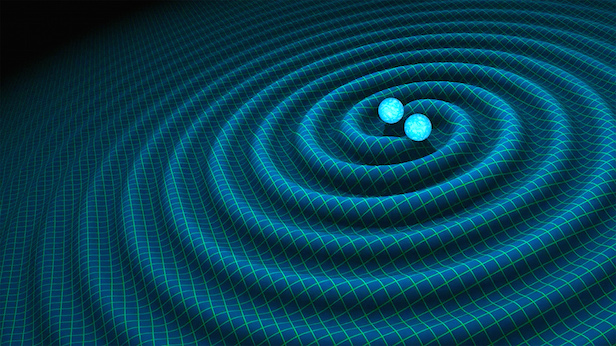
\includegraphics[width=0.8\textwidth]{figures/Gravity/waves}};
\node at (-2cm,-2cm) {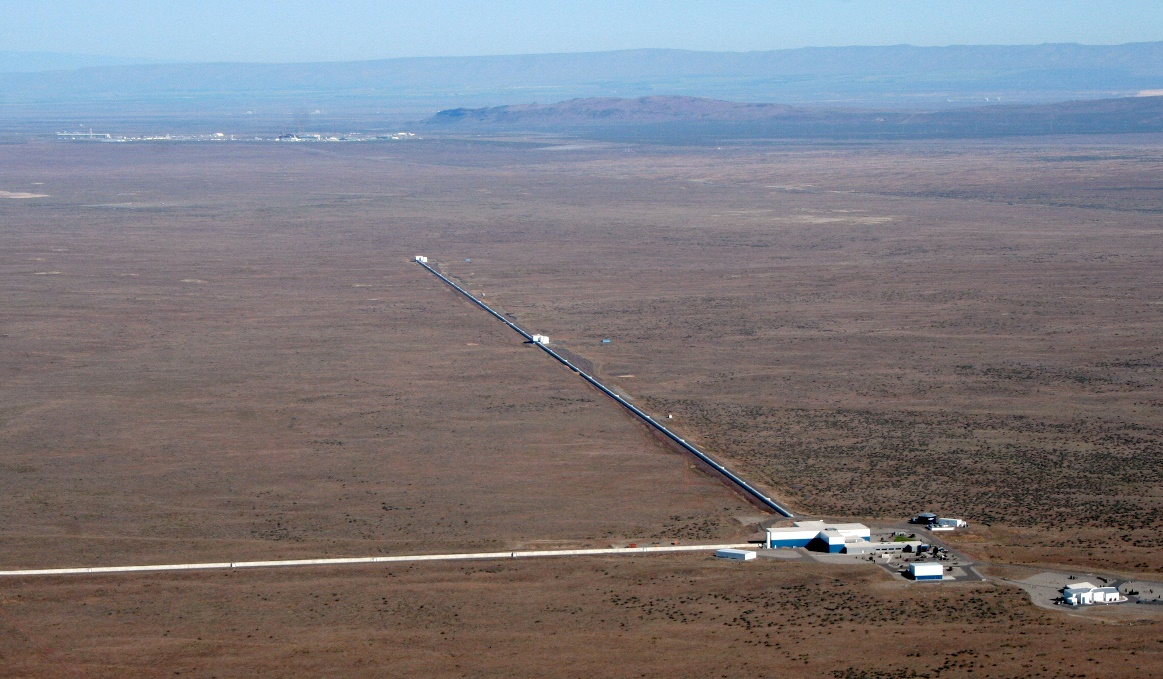
\includegraphics[width=0.8\textwidth]{figures/Gravity/ligo}};
\node at (0.7,-1cm) {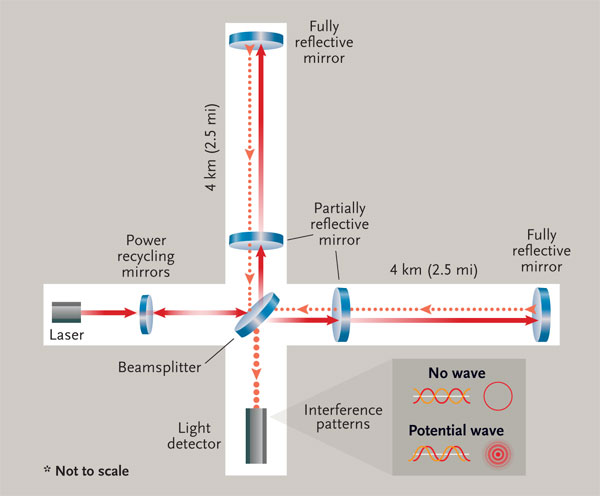
\includegraphics[width=0.45\textwidth]{figures/Gravity/interferometer}};
\end{tikzpicture}
\captionof*{figure}{\textit\tiny{Daw, E. (2016, February 11). Gravitational waves discovered: How did the experiment at LIGO actually work? The Conversation. https://theconversation.com/gravitational-waves-discovered-how-did-the-experiment-at-ligo-actually-work-54510,
\\
Gravitational Wave Detection Heralds New Era. (n.d.). Sky \& Telescope. https://skyandtelescope.org/astronomy-news/gravitational-wave-detection-heralds-new-era-of-science-0211201644}}
\end{center}
}


%%%%%%%%%%%%%%%%%%%%%%%%%%%%%%%%
\begin{frame}{Issues with GR}
\begin{itemize}
\item Mathematically, it is very different from the theories for the other 3 forces of nature – it’s not clear how to combine it into a unified theory of physics (in particular, the ``quantum'' aspect).
\item It has some unusual consequences:
\begin{itemize}
\item Most of the energy (70\%) in the Universe is a ``negative energy'' (``Dark energy'') that is responsible for the Universe expanding $\rightarrow$ we know this from measuring the curvature of space and rate of expansion.
\item Most of the matter in the Universe is in a non-luminous form that we have never detected (``Dark Matter'') $\rightarrow$ we are trying to detect it; we think it's just a different type of particle.
\end{itemize}
\end{itemize}
\end{frame}

%%%%%%%%%%%%%%%%%%%%%%%%%%%%%%%%
































%%%%%%%%%%%%%%%%%%%%%%%%%%%%%%%%



\title{Momentum and Centre of Mass}
\subject{Systems, Collisions and Centre of Mass}
\subtitle{Building Models to Describe our World}




%%%%%%%%%%%%%%%%%%%%%%%%%
%%%%%% Title slide %%%%%%
%%%%%%%%%%%%%%%%%%%%%%%%%
\chaptertitle{Momentum and Centre of Mass}
\begin{frame}
\label{chap:momentumandcm}
\titlepage
\thispagestyle{empty}

\begin{textblock*}{5cm}(11cm,4cm)
    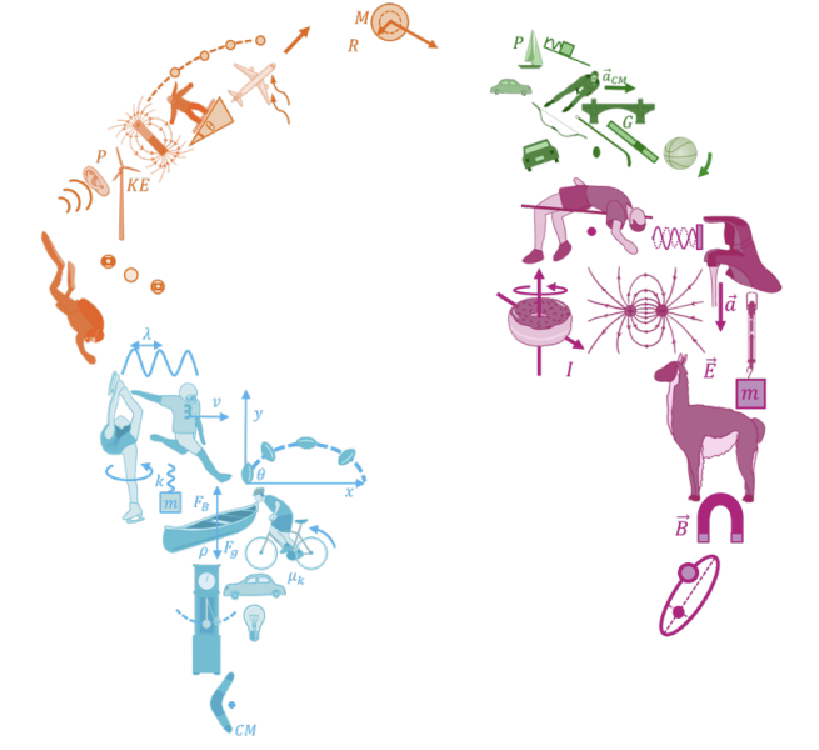
\includegraphics[width=4cm]{figures/BMDW/logo}
\end{textblock*}

\end{frame}

%%%%%%%%%%%%%TOC

\twocolframe{Outline}
{\tableofcontents[sections=25-26, subsectionstyle=show/show]\thispagestyle{empty}}
{\tableofcontents[sections=27, subsectionstyle=show/show]}

%%%%%%%%%%%%%%%%%%%%%%%%%









%%%%%%%%%%%%%%%%%%%%%%%%%%%%%%%%
\section{Momentum Basics}
\label{sec:momentumbasics}
\title{Momentum Basics}
\institute{Momentum and Centre of Mass}
\author{\insertsubsection}


%%%%%%%%%%%%%%%%%%%%%%%%%
\begin{frame}
\titlepage
\thispagestyle{empty}
\end{frame}

%%%%%%%%%%%%%%













%%%%%%%%%%%%%%%%%%%%%%%%%%%%
\subsection{Momentum of  a particle}
\label{subsec:momentumofaparticle}
\begin{frame}{Momentum of a particle}
\begin{itemize}
\item The momentum of a particle of mass $m$ is:
\begin{align*}
\vec p = m \vec v
\end{align*}
\item The rate of change of momentum is the net force on the particle:
\begin{align*}
\frac{d\vec p}{dt} &= \frac{d}{dt}m\vec v= m\frac{d\vec v}{dt} = m\vec a\\
\therefore \frac{d\vec p}{dt} &= \sum \vec F = \vec F^{net}
\end{align*}
\item \textbf{If the net force on a particle is zero, its momentum is constant} (it doesn't change with time).
\end{itemize}

\end{frame}


%%%%%%%%%%%%%%%%%%%%%%%%%%%%%%%%



%%%%%%%%%%%%%%%%%%%%%%%%%%%%%%%%
\subsection{Impulse}
\label{subsec:impulse}
\twocolframesf{Impulse}
{
\vspace{-0.5cm}
\begin{itemize}
\item The net impulse \textbf{vector} is the change in momentum:
\begin{itemize}
\item If force does not change with time:
\begin{align*}
\frac{d\vec p}{dt} &\sim\frac{\Delta \vec p}{\Delta t} =\vec F^{net}\\
\therefore \vec J^{net} &= \Delta \vec p=\vec F^{net} \Delta t
\end{align*}
\item If force changes magnitude or direction with time
\begin{align*}
\vec J^{net} = \Delta \vec p = \int_{t_a}^{t_b}\vec F^{net}(t) dt
\end{align*}
\end{itemize}
\item A force acting for a given time will change the momentum.
\item \textit{What makes it different from Work}?
\end{itemize}
}
{
\begin{center}
\begin{tikzpicture}
\tikzmath{
\L=2;
\h=3;
}
\scalebox{1}{
\coordinate (P1) at (0,0);
\coordinate (C1) at (\h,\L/2);
\coordinate (P2) at (\L,\h);

\draw[line width=1, dashed] (P1) node[above]{$A$} .. controls (C1) .. (P2) node[right]{$B$};
\draw[-latex, line width =1.5] (P1) -- ($(P1)!0.3!(C1)$) node[below]{$\vec p_A$};
\draw[-latex, line width =1.5] (P2) -- ($(P2)!-0.3!(C1)$) node[above]{$\vec p_B$};

\begin{scope}[shift={(0,1.5)}]

\draw[-latex, line width =1.5] (0,0) -- ($(0,0)!0.3!(\h,\L/2)$) node[below]{$\vec p_A$};
\draw[-latex, line width =1.5, color=myred] ($(0,0)!0.3!(\h,\L/2)$) -- ($ (\L,\h)!-0.3!(\h,\L/2)-(\L,\h)$) node[midway,above]{$\vec J^{net}$};
\end{scope}

\begin{scope}[shift={(-\L,1.5-\h)}]
\draw[-latex, line width =1.5] (\L,\h) -- ($(\L,\h)!-0.3!(\h,\L/2)$) node[left]{$\vec p_B$};
\end{scope}

\begin{scope}[shift={(\h,\L/2)}]
\draw[-latex, line width =1.5] ($(0,0)!0.3!(\h,\L/2)$)node[above]{$\vec F^{net}$} -- ($ (\L,\h)!-0.3!(\h,\L/2)-(\L,\h)$) ;
\end{scope}

}
\end{tikzpicture}
\captionof*{figure}{\textit{Impulse is the change in momentum.}}
\end{center}
\begin{align*}
\vec J^{net}=\Delta \vec p=\vec p_B-\vec p_A = \vec F^{net}\Delta t
\end{align*}
}


%%%%%%%%%%%%%%%%%%%%%%%%%%%%%%%%


%%%%%%%%%%%%%%%%%%%%%%%%%%%%%%%%
\subsection{Systems of particles}
\label{subsec:systemsofparticles}
\begin{frame}{Systems of particles}
\begin{itemize}
\item Newton’s Second Law is only valid for a point particle (an infinitely small particle of mass, $m$).
\item Loosely, we call a collection of particles a ``system''.
\item A solid block of matter is a system of many particles that cannot move relative to each other.
\item A gas is a system of many particles that can move relative to each other.
\item So far, we have modelled, say, blocks and treated them like point particles even if they are not.
\item We can distinguish between ``internal'' and ``external'' forces to the system.
\end{itemize}
\end{frame}


%%%%%%%%%%%%%%%%%%%%%%%%%%%%%%%%


%%%%%%%%%%%%%%%%%%%%%%%%%%%%%%%%
\twocolframesf{Modeling 2 blocks as a system}
{
\only<1>{
\begin{itemize}
\item Want to know the acceleration of the two blocks, given $F$, friction.
\item Can apply Newton's Second Law to each block (4 equations, blocks have the same acceleration):
\begin{align*}
\sum F_1^{horiz}&=T-\mu_k N_1=m_1a\\
\sum F_2^{horiz}&=F-T-\mu_k N_2=m_2a\\
&+\text{forces in vertical direction}
\end{align*}
\end{itemize}
}
\only<2>{
\begin{itemize}
\item But, the motion of the system, $(m_1+m_2)$, depends on the external forces on the system. Tension is an \textit{internal} force.
\item Consider adding together Newton’s Second Law for each particle:
\begin{align*}
\sum F_1^{horiz}=T-\mu_k N_1&=m_1a\\
\sum F_2^{horiz}=F-T-\mu_k N_2&=m_2a\\
\sum F_1^{horiz} + \sum F_2^{horiz}&=\textcolor{myred}{T}-\mu_k N_1+F\textcolor{myred}{-T}-\mu_k N_2\\
\therefore F-\mu_k(N_1+N_2)&=(m_1+m_2)a\\
F-\mu_k(m_1+m_2)g&=(m_1+m_2)a
\end{align*}
\end{itemize}
}
}
{
\begin{center}
\vspace{-1cm}
\begin{tikzpicture}
\tikzmath{
\L=5;
\abox=1;
}

\scalebox{1}{
\fill (0,-0.1) rectangle (\L,0);

\fill[color=myblue!60] (0.5,0) rectangle +(\abox,\abox);
\fill[color=myblue!60] (2.5,0) rectangle +(\abox,\abox);
\node[above] at (0.5+\abox/2,\abox) {$m_1$};
\node[above] at (2.5+\abox/2,\abox) {$m_2$};
\draw[line width=1] (0.5+\abox,\abox/2) -- +(1,0);
\draw[-latex,line width=2] (2.5+\abox,\abox/2) -- +(1,0) node[midway,above]{$\vec F$};

\begin{scope}[shift={(0,-3)}]
\coordinate (P1) at (0.5+\abox/2,\abox);
\coordinate (P2) at (2.5+\abox/2,\abox);

\fill (P1) circle (2pt);
\fill (P2) circle (2pt);

\draw[-latex, line width=2] (P1) -- +(-0.5,0) node[above]{$\vec f_{k1}$};
\draw[-latex, line width=2] (P2) -- +(-0.6,0) node[above]{$\vec f_{k2}$};

\draw[-latex, line width=2] (P1) -- +(0.75,0) node[above]{$\textcolor{myred}{\vec T}$};
\draw[-latex, line width=2] ($(P2)-(0,0.2)$) -- +(-0.75,0) node[below]{$\textcolor{myred}{-\vec T}$};
\draw[-latex, line width=2] ($(P2)$) -- +(1,0) node[below]{$\vec F$};

\draw[-latex, line width=2] (P1) -- +(0,0.9) node[above]{$\vec N_{1}$};
\draw[-latex, line width=2] (P2) -- +(0,1.1) node[above]{$\vec N_{2}$};

\draw[-latex, line width=2] (P1) -- +(0,-0.9) node[left]{$\vec F_{g1}$};
\draw[-latex, line width=2] (P2) -- +(0,-1.1) node[right]{$\vec F_{g2}$};

\end{scope}

}
\end{tikzpicture}
\captionof*{figure}{\textit{Modeling two connected blocks, either individually or as a system.}}
\end{center}
\only<2>{
\scriptsize
The internal forces (exerted by one object of the system on another) always cancel out because of Newton’s Third Law. Only the external forces affect the motion of the system.
}
}


%%%%%%%%%%%%%%%%%%%%%%%%%%%%%%%%
\subsection{Momentum of a system}
\label{subsec:momentumofasystem}
\begin{frame}{Momentum of a system}
\begin{itemize}
\item If many particles make up a system, we can add their individual momenta together to define the total momentum of the system:
\begin{align*}
\vec P = \vec p_1 + \vec p_2 +\vec p_3+\dots
\end{align*}
\item The rate of change of momentum of the system is given by the sum of the \textbf{external forces} exerted on the system:
\begin{align*}
\frac{d\vec P}{dt}=\frac{d\vec p_1}{dt} + \frac{d\vec p_2}{dt}  + \frac{d\vec p_3}{dt} +\dots=  \sum \vec F ^{ext}
\end{align*}
\item If there is \textbf{no net external force on the system, the momentum of the system is conserved}.
\end{itemize}
\end{frame}


%%%%%%%%%%%%%%%%%%%%%%%%%%%%%%%%








%%%%%%%%%%%%%%%%%%%%%%%%%%%%%%%%
\section{Collisions}
\label{sec:collisions}
\title{Collisions}
\institute{Momentum and Centre of Mass}
\author{\insertsubsection}


%%%%%%%%%%%%%%%%%%%%%%%%%
\begin{frame}
\titlepage
\thispagestyle{empty}
\end{frame}

%%%%%%%%%%%%%%











%%%%%%%%%%%%%%%%%%%%%%%%%%%%%%%%
\subsection{Concept}
\label{subsec:collisionconcept}
\twocolframesf{Collisions}
{
\begin{itemize}
\item ``Events'' where one considers the total momentum of a system ``just before'' and ``just after''.
\item Examples:
\begin{itemize}
\item Billiard balls colliding.
\item An arrow embedding itself into a block of wood that can move.
\item A bomb exploding into fragments.
\end{itemize}
\item Even if there are net external forces (e.g. gravity), one can \textbf{usually} neglect them if the momentum is compared just before and just after the collision and model total momentum as being conserved.
\end{itemize}
}
{
\begin{center}
\begin{tikzpicture}
\tikzmath{
\L=5;
\h=\L/2;
\w=6;
}

\scalebox{1}{
%table
\fill[color=poolgreen, draw=brown, line width=5pt] (0,0) rectangle (\L,\h);
%pockets
\fill (0,0) circle(3pt);.
\fill (0,\h) circle(3pt);
\fill (\L/2,0) circle(3pt);
\fill (\L/2,\h) circle(3pt);
\fill (\L,0) circle(3pt);
\fill (\L,\h) circle(3pt);
%balls
\shade[ball color=white,opacity=0.5] (\L/2-0.4,\h/2) circle(2.5pt);
\shade[ball color=white,opacity=0.6] (\L/2-0.25,\h/2) circle(2.5pt);
\shade[ball color=white,opacity=0.7] (\L/2-0.15,\h/2) circle(2.5pt);
\shade[ball color=white] (\L/2,\h/2) circle(2.5pt);

\shade[ball color=black,opacity=0.3] (\L/2+0.2,\h/2+0.1) circle(2.5pt);
\shade[ball color=black,opacity=0.4] (\L/2+0.4,\h/2+0.2) circle(2.5pt);
\shade[ball color=black,opacity=0.5] (\L/2+0.6,\h/2+0.3) circle(2.5pt);
\shade[ball color=black] (\L/2+0.8,\h/2+0.4) circle(2.5pt);

\shade[ball color=purple,opacity=0.3] (\L/2+0.2,\h/2-0.1) circle(2.5pt);
\shade[ball color=purple,opacity=0.4] (\L/2+0.3,\h/2-0.2) circle(2.5pt);
\shade[ball color=purple,opacity=0.5] (\L/2+0.4,\h/2-0.3) circle(2.5pt);
\shade[ball color=purple] (\L/2+0.5,\h/2-0.4) circle(2.5pt);
}
\end{tikzpicture}
\captionof*{figure}{\textit{Billiard balls colliding.}}
\end{center}

\begin{center}
\begin{tikzpicture}
\tikzmath{
\R=0.75;
}

\scalebox{1}{
\shade[ball color=black] (0,0) circle(\R);
\node [star, star points=6, star point ratio=0.5, minimum size=0.05cm, fill=yellow!60!orange]
       at (0.6*\R,1.3*\R){};
\draw[line width=1.5pt, color=brown] plot [smooth] coordinates {(0,\R) (0.1*\R,1.2*\R)  (0.4*\R,1.1*\R) (0.6*\R,1.3*\R) };

\begin{scope}[shift={(3cm,0)}]
%\draw (45:1.2*\R) circle(4pt);

\fill[top color=black, bottom color=black!60] (45:0.7*\R) -- ($(45:0.7*\R)+(0.3*\R,0.2*\R)$) -- ($(45:0.7*\R)+(\R,0)$) arc(0:90:\R) -- ($(45:0.7*\R)+(0.2*\R,0.5*\R)$) --cycle ;
\fill[top color=black, bottom color=black!40] (135:0.4*\R) -- ($(135:0.4*\R)+(0.2*\R,0.5*\R)$) -- ($(135:0.4*\R)+(0,\R)$) arc(90:180:\R) -- ($(135:0.4*\R)+(-0.8*\R,0.2*\R)$)--cycle ;
\fill[bottom color=black, top color=black!40] (225:0.5*\R) -- ($(225:0.5*\R)+(-0.8*\R,0.2*\R)$) -- ($(225:0.5*\R)+(-\R,0)$) arc(180:270:\R) -- ($(225:0.5*\R)+(-0.5*\R,-0.3*\R)$)  --cycle;
\fill[bottom color=black, top color=black!60] (315:0.3*\R) -- ($(315:0.3*\R)+(-0.5*\R,-0.3*\R) $) -- ($(315:0.3*\R)+(0,-\R) $)arc(-90:0:\R) -- ($(315:0.3*\R)+(0.3*\R,0.2*\R) $)  --cycle ;

\draw [-latex, line width=1] (45:1.7*\R) -- +(45:0.7*\R);
\draw [-latex, line width=1] (135:1.4*\R) -- +(135:0.4*\R);
\draw [-latex, line width=1] (225:1.5*\R) -- +(225:0.5*\R);
\draw [-latex, line width=1] (315:1.3*\R) -- +(315:0.3*\R);

\end{scope}


}
\end{tikzpicture}
\captionof*{figure}{\textit{An explosion.}}
\end{center}
}

%%%%%%%%%%%%%%%%%%%%%%%%%%%%%%%%


%%%%%%%%%%%%%%%%%%%%%%%%%%%%%%%%
\subsection{Elastic vs inelastic}
\label{subsec:elasticvinelastic}
\begin{frame}{Elastic vs Inelastic}
\begin{itemize}
\item Just because momentum is conserved does not mean that mechanical energy is conserved:
\begin{itemize}
\item \textbf{Momentum }is conserved when there is \textbf{no net external force} on the system.
\item \textbf{Energy} is conserved when there is \textbf{no non-conservative force} doing work on any particle in the system.
\end{itemize}
\item To model elastic collisions, the mechanical energy of the system is conserved before and after the collision:
\begin{align*}
E=K+U=K'+U'=E'
\end{align*}
\item $K$, $U$ are the total kinetic energy and total potential energy of the system (add together the kinetic and potential energies of all particles in the system).
\item Usually, if the collision happens over a small distance, then the potential energies are (almost) the same before and after the collision (potential energy depends on position and if position doesn’t change much, neither does $U$):
\begin{align*}
U=U'\quad \text{(Usually)}
\end{align*}
\end{itemize}
\end{frame}


%%%%%%%%%%%%%%%%%%%%%%%%%%%%%%%%
\subsection{Elastic collision in 1D}
\label{subsec:elasticcollisionin1d}
\twocolframesf{Elastic collision in 1D: $m$ collides with $m$ at rest}
{
\vspace{-0.25cm}
\begin{itemize}
\item<1-> Conservation of momentum:
\begin{align*}
m\vec v_1=m\pvec v_1'+m \pvec v_2'
\end{align*}
\item<2-> $x$-component:
\begin{align*}
 \Aboxed{v_1= v_1'+v_2'}
\end{align*}
\item<3-> Conservation of energy:
\begin{align*}
\frac{1}{2}mv_1^2&=\frac{1}{2}m{v'}_1^{2}+\frac{1}{2}m{v'}_2^{2}\\
\therefore \Aboxed{v_1^2&= {v'}_1^{2}+ {v'}_2^{2}}
\end{align*}
\item<3-> 2 equations 2 unknowns, but not trivial, since not linear (i.e. quadratic)
\end{itemize}
}
{
\begin{center}
\begin{tikzpicture}
\tikzmath{
\L=5;
\abox=0.75;
}

\scalebox{1}{
\fill (0,-0.1) rectangle (\L,0);

\fill[color=myblue!60] (0.5,0) rectangle +(\abox,\abox);
\fill[color=myblue!60] (2.5,0) rectangle +(\abox,\abox);
\node[above] at (0.5+\abox/2,\abox) {$m$};
\node[above] at (2.5+\abox/2,\abox) {$m$};
\draw[-latex,line width=2] (0.5+\abox,\abox/2) -- +(0.75,0) node[midway,above]{$\vec v_1$};

\begin{scope}[shift={(0,-1.5)}]
\fill (0,-0.1) rectangle (\L,0);
\fill[color=myblue!60] (1,0) rectangle +(\abox,\abox);
\fill[color=myblue!60] (3,0) rectangle +(\abox,\abox);
\node[above] at (1+\abox/2,\abox) {$m$};
\node[above] at (3+\abox/2,\abox) {$m$};
\draw[-latex,line width=2] (1,\abox/2) -- +(-0.5,0) node[midway,above]{$\pvec v'_1$};
\draw[-latex,line width=2] (3+\abox,\abox/2) -- +(1,0) node[midway,above]{$\pvec v'_2$};
\draw[-latex] (0,-0.3) -- +(\L,0) node[below]{$x$};
\end{scope}

}
\end{tikzpicture}
\captionof*{figure}{\textit{A block of mass, $m$, with speed $v_1$, collides elastically with another block of mass, $m$, initially at rest.}}
\end{center}
}


%%%%%%%%%%%%%%%%%%%%%%%%%%%%%%%%
\begin{frame}{Useful trick for elastic collisions}
\begin{itemize}
\item Instead of writing ``before''= ``after'':
\begin{align*}
v_1&= v_1'+v_2'\\
v_1^2&= {v'}_1^{2}+ {v'}_2^{2}
\end{align*}
\item Write ``1'' = ``2'':
\begin{align}
v_1-v_1'&=v_2'\\
v_1^2-{v'}_1^{2}&= {v'}_2^{2}\\
\therefore (v_1-v'_1)(v_1+v'_1)&={v'}_2^{2}\quad\text{(factoring equation 2)}
\end{align}
\item Divide equation 3 by equation 1:
\begin{align*}
\frac{(v_1-v'_1)(v_1+v'_1)}{v_1-v_1'}=v'_2\quad \rightarrow \quad \Aboxed{v_1+v'_1 = v'_2}
\end{align*}
\end{itemize}

\end{frame}


%%%%%%%%%%%%%%%%%%%%%%%%%%%%%%%%
\twocolframesf{Elastic collision in 1D: $m$ collides with $m$ at rest}
{
\begin{itemize}
\item Solve for the final velocities:
\begin{align*}
v_1-v_1'&=v_2'\\
v_1+v'_1 &= v'_2
\end{align*}
\item Which gives:
\begin{align*}
v'_1&=0\\
v'_2&=v_1
\end{align*}
The first block comes to rest and the second one moves with the same speed as the first one did!
\end{itemize}
}
{
\begin{center}
\begin{tikzpicture}
\tikzmath{
\L=5;
\abox=0.75;
}

\scalebox{1}{
\fill (0,-0.1) rectangle (\L,0);

\fill[color=myblue!60] (0.5,0) rectangle +(\abox,\abox);
\fill[color=myblue!60] (2.5,0) rectangle +(\abox,\abox);
\node[above] at (0.5+\abox/2,\abox) {$m$};
\node[above] at (2.5+\abox/2,\abox) {$m$};
\draw[-latex,line width=2] (0.5+\abox,\abox/2) -- +(0.75,0) node[midway,above]{$\vec v_1$};

\begin{scope}[shift={(0,-1.5)}]
\fill (0,-0.1) rectangle (\L,0);
\fill[color=myblue!60] (2.5,0) rectangle +(\abox,\abox);
\fill[color=myblue!60] (3.5,0) rectangle +(\abox,\abox);
\node[above] at (2.5+\abox/2,\abox) {$m$};
\node[above] at (3.5+\abox/2,\abox) {$m$};

\draw[-latex,line width=2] (3.5+\abox,\abox/2) -- +(0.75,0) node[midway,above]{$\vec v_1$};
\draw[-latex] (0,-0.3) -- +(\L,0) node[below]{$x$};
\end{scope}

}
\end{tikzpicture}
\captionof*{figure}{\textit{A block of mass, $m$, with speed $v_1$, collides elastically with another block of mass, $m$, initially at rest.}}
\end{center}
}


%%%%%%%%%%%%%%%%%%%%%%%%%%%%%%%%


%%%%%%%%%%%%%%%%%%%%%%%%%%%%%%%%
\subsection{How to identify an elastic collision}
\label{subsec:howtoidentifyanelasticcollision}
\begin{frame}{How to tell if it is elastic?}
\begin{itemize}
\item Calculate the initial and final kinetic energies and compare them. 
\begin{itemize}
\item Problem solving hint: If you are given enough information to be able to calculate the initial and final velocities using only conservation of momentum, chances are it was inelastic...
\end{itemize}
\item If two objects stick together, or come unstuck (e.g. explosion), then the energy is not conserved:
\begin{itemize}
\item Think of two equal masses coming towards each other at the same speed and coming to rest stuck together. The total momentum is always zero, but the total kinetic energy went from non-zero to zero.
\end{itemize}
\item If you are told about the collision mechanism, you might be able to determine if it’s elastic. E.g. colliding with a spring is elastic (that’s where the term comes from).
\end{itemize}
\end{frame}


%%%%%%%%%%%%%%%%%%%%%%%%%%%%%%%%


%%%%%%%%%%%%%%%%%%%%%%%%%%%%%%%%
\subsection{Example: basketball and tennis ball}
\label{subsec:basketballandtennisball}
\twocolframesf{Basketball and tennis ball}
{

\only<1-2>{
\begin{itemize}
\item Just before the collision,  assume that tennis ball speed = basketball speed. Assume elastic collision (between balls and with the ground).
\item Work it out... you will find:
\begin{align*}
v'_t = \frac{3M-m}{M+m}v
\end{align*}
\item<2-> Re-write as (divide through by $M$):
\begin{align*}
v'_t = \frac{3-\frac{m}{M}}{1+\frac{m}{M}}v
\end{align*}
\item<2-> If $M>>m$, $\frac{m}{M}\sim 0$ and $v'_t\sim 3 v$. 
\end{itemize}
}
\only<3->{
\begin{itemize}
\item<3-> If $M>>m, \frac{m}{M}\sim 0$:
\begin{align*}
v'_t = \frac{3-\frac{m}{M}}{1+\frac{m}{M}}v\sim 3v
\end{align*}
\item<4> With speed $v$, the tennis ball will go a height $h$:
\begin{align*}
mgh&=\frac{1}{2}mv^2\\
\therefore h &\propto v^2
\end{align*}
The height of the bounce goes as speed squared: the tennis ball will bounce to 9$\times$ than from where it was released.
\end{itemize}


}
}
{
\vspace{-1cm}
\begin{center}
\begin{tikzpicture}
\tikzmath{
\h=3;
}

\scalebox{1}{
\node at (0,0) {
\includegraphics[scale=0.5]{figures/MomentumAndCM/bball}};
\node at (0,\h) {
\includegraphics[scale=0.5]{figures/MomentumAndCM/tball}};
\draw[-latex, line width=1.5] (0,\h) -- +(0,-1) node[midway,right]{$-\vec v$};
\draw[-latex, line width=1.5] (0,0.75) -- +(0,1) node[left]{$\vec v$};

\begin{scope}[shift={(2,0)}]
\node at (0,0) {
\includegraphics[scale=0.5]{figures/MomentumAndCM/bball}};
\node at (0,\h) {
\includegraphics[scale=0.5]{figures/MomentumAndCM/tball}};
\draw[-latex, line width=1.5] (0,\h) -- +(0,2) node[left]{$\pvec v'_t$};
\draw[-latex, line width=1.5] (0,0.75) -- +(0,1) node[left]{$\pvec v'_b$};
\end{scope}
}
\end{tikzpicture}
\captionof*{figure}{\textit{A basketball colliding with a tennis ball.}}
\end{center}
}


%%%%%%%%%%%%%%%%%%%%%%%%%%%%%%%%
\subsection{Ballistic pendum}
\label{subsec:ballisticpendulum}
\twocolframesf{Ballistic pendulum}
{
\begin{itemize}
\item The bullet/arrow embeds itself in the pendulum block.
\item The pendulum rises.
\item The height allows you to determine the speed of the arrow.
\end{itemize}
}
{
\begin{center}
\begin{tikzpicture}
\tikzmath{
\Lc=2;
\L=1.5;
\h=0.25;
\boxh=0.5;
\boxL=1;
\ropew=0.5*\boxL;
\dis=0.75;
}

\scalebox{1}{

\fill (-\Lc/2,0) rectangle (\Lc/2,0.05);
\draw (-\ropew/2,0) -- +(0,-\L);
\draw (\ropew/2,0) -- +(0,-\L) node[midway,right]{$L=\SI{0.75}{m}$};
\fill[color=myblue!60] (-\boxL/2,-\L) rectangle (\boxL/2,-\L-\boxh);
\draw[color=myred, line width=2,latex-] (\boxL/2+\dis,-\L-\boxh/2) -- +(1,0) node[midway,above]{$m=\SI{100}{g}$}node[midway,below]{$v$};
\node[below] at (0,-\L-\boxh) {$M=\SI{2.756}{kg}$};

\begin{scope}[shift={(0,-3)}]
\fill (-\Lc/2,0) rectangle (\Lc/2,0.05);
\draw (-\ropew/2,0) -- +(-\dis,-\L);
\draw (\ropew/2,0) -- +(-\dis,-\L) node[midway,left]{\scriptsize $L$};

\fill[color=myblue!60] (-\boxL/2-\dis,-\L) rectangle (\boxL/2-\dis,-\L-\boxh);
\draw[color=myred, line width=2,latex-] (-\boxL/2-0.75*\dis,-\L-\boxh/2) -- +(1,0) ;

\draw[dashed] (\ropew/2,0) -- +(0,-\L-\h) node[midway,right]{\scriptsize $L$};
\draw[latex-latex, line width=1] (\ropew/2,-\L+0.1) -- +(-\dis,0) node[midway,above]{$d$};
\draw[latex-latex, line width=0.5] (\ropew/2,-\L-\h) -- +(0,0.1+\h) node[midway,right]{\scriptsize $h=L-\sqrt{L^2-d^2}$};
\end{scope}

}
\end{tikzpicture}
\captionof*{figure}{\textit{An arrow embeds itself into a ballistic pendulum.}}
\end{center}
}


%%%%%%%%%%%%%%%%%%%%%%%%%%%%%%%%

%%%%%%%%%%%%%%%%%%%%%%%%%%%%%%%%
\twocolframesf{Exercise: Find the speed of the arrow, given $d$.}
{
\begin{itemize}
\item<2-> Conservation of momentum (inelastic collision):
\begin{align*}
mv=(M+m)v'
\end{align*}
\item<3-> Conservation of energy after the collision:
\begin{align*}
\frac{1}{2}(M+m){v'}^2=(M+m)gh
\end{align*}
\item<4-> You should find:
\begin{align*}
v &= \frac{M+m}{m}\sqrt{2g\left(L-\sqrt{L^2-d^2}\right)}\\
&= (28.56)\sqrt{(\SI{19.6}{m/s^2})\left((\SI{0.75}{m})-\sqrt{(\SI{0.75}{m})^2-d^2}\right)}
\end{align*}
\end{itemize}
}
{
\begin{center}
\begin{tikzpicture}
\tikzmath{
\Lc=2;
\L=1.5;
\h=0.25;
\boxh=0.5;
\boxL=1;
\ropew=0.5*\boxL;
\dis=0.75;
}

\scalebox{1}{

\fill (-\Lc/2,0) rectangle (\Lc/2,0.05);
\draw (-\ropew/2,0) -- +(0,-\L);
\draw (\ropew/2,0) -- +(0,-\L) node[midway,right]{$L=\SI{0.75}{m}$};
\fill[color=myblue!60] (-\boxL/2,-\L) rectangle (\boxL/2,-\L-\boxh);
\draw[color=myred, line width=2,latex-] (\boxL/2+\dis,-\L-\boxh/2) -- +(1,0) node[midway,above]{$m=\SI{100}{g}$} node[midway,below]{$v$};
\node[below] at (0,-\L-\boxh) {$M=\SI{2.756}{kg}$};

\begin{scope}[shift={(0,-3)}]
\fill (-\Lc/2,0) rectangle (\Lc/2,0.05);
\draw (-\ropew/2,0) -- +(-\dis,-\L);
\draw (\ropew/2,0) -- +(-\dis,-\L) node[midway,left]{\scriptsize $L$};

\fill[color=myblue!60] (-\boxL/2-\dis,-\L) rectangle (\boxL/2-\dis,-\L-\boxh);
\draw[color=myred, line width=2,latex-] (-\boxL/2-0.75*\dis,-\L-\boxh/2) -- +(1,0) ;

\draw[dashed] (\ropew/2,0) -- +(0,-\L-\h) node[midway,right]{\scriptsize $L$};
\draw[latex-latex, line width=1] (\ropew/2,-\L+0.1) -- +(-\dis,0) node[midway,above]{$d$};
\draw[latex-latex, line width=0.5] (\ropew/2,-\L-\h) -- +(0,0.1+\h) node[midway,right]{\scriptsize $h=L-\sqrt{L^2-d^2}$};
\end{scope}

}
\end{tikzpicture}
\captionof*{figure}{\textit{An arrow embeds itself into a ballistic pendulum.}}
\end{center}
}

%%%%%%%%%%%%%%%%%%%%%%%%%%%%%%%%








%%%%%%%%%%%%%%%%%%%%%%%%%%%%%%%%
\section{Centre of Mass}
\label{sec:centreofmass}
\title{Centre of Mass}
\institute{Momentum and Centre of Mass}
\author{\insertsubsection}


%%%%%%%%%%%%%%%%%%%%%%%%%
\begin{frame}
\titlepage
\thispagestyle{empty}
\end{frame}

%%%%%%%%%%%%%%









%%%%%%%%%%%%%%%%%%%%%%%%%%%%%%%%
\subsection{Describing a system}
\label{subsec:describingasystem}
\begin{frame}{Describing a system}
\begin{itemize}
\item We can define a system of particles; that system can be particles that are freely moving with respect to each other, or it could be a solid object.
\item We found that the motion of the system as a whole is determined by the external forces on the system (the internal forces cancel out).
\item Want to define some quantities that allow us to describe the motion of the system as a whole:
\begin{itemize}
\item Total momentum $\rightarrow$ add momenta of particles in the system.
\item Total energy (kinetic + potential) $\rightarrow$ add energies of particles in the system.
\item Position $\rightarrow$ figure out some average position of the system (the CM).
\end{itemize}

\end{itemize}

\end{frame}


%%%%%%%%%%%%%%%%%%%%%%%%%%%%%%%%
\twocolframesf{Describing a system}
{
\begin{itemize}
\item The total momentum of a system:
\begin{align*}
\vec P=\vec p_1 + \vec p_2 + \vec p_3 + \dots
\end{align*}
is conserved if there are no net external forces:
\begin{align*}
\frac{d\vec P}{dt}=\sum_{system} \vec F^{ext}
\end{align*}
\item Want to write Newton’s 2nd Law, using the \textbf{total mass of the system}, $M$:
\begin{align*}
\sum_{system} \vec F^{ext}=M\vec a_{CM}
\end{align*}

\item But, $a_{CM}$, is the acceleration of what??

\end{itemize}
}
{
\vspace{-1cm}
\begin{center}
\begin{tikzpicture}

\scalebox{1}{

\coordinate (P1) at (0,0);
\coordinate (P2) at (1.5,1);
\coordinate (P3) at (1,2);
\coordinate (P4) at (3,2);
\coordinate (P5) at (4,1);
\coordinate (P) at (2.75,1);
\fill (P1) circle (2pt);
\fill (P2) circle (2pt);
\fill (P3) circle (2pt);
\fill (P4) circle (2pt);
\fill (P5) circle (2pt);

\draw[-latex, line width=1] (P1) -- +(110:0.75) node[left]{$\vec p_1$};
\draw[-latex, line width=1] (P2) -- +(160:0.5) node[below]{$\vec p_2$};
\draw[-latex, line width=1] (P3) -- +(80:0.6) node[right]{$\vec p_3$};
\draw[-latex, line width=1] (P4) -- +(135:0.9) node[above]{$\vec p_4$};
\draw[-latex, line width=1] (P5) -- +(100:0.5) node[above]{$\vec p_5$};

\draw[-latex, line width=2] (P) -- ($(P)+(110:0.75)+(160:0.5)+(80:0.6)+(135:0.9)+(100:0.5)$) node[above]{$\vec P$};
}
\end{tikzpicture}
\captionof*{figure}{\textit{The momentum of a system of particles is given by the sum of the individual momenta of the particles.}}
\end{center}
\scriptsize
For one particle:
\begin{align*}
\frac{d\vec p_i}{dt}=\sum \vec F=m\vec a = m\frac{d\vec v}{dt}=m\frac{d^2\vec r}{dt^2}
\end{align*}
}


%%%%%%%%%%%%%%%%%%%%%%%%%%%%%%%%
\subsection{Concept}
\label{subsec:conceptcm}
\begin{frame}{Centre of mass}
\begin{itemize}
\item We define the centre of mass of a system to be that \textbf{location in the system that is described by}:
\begin{align*}
\sum_{system} \vec F^{ext}=M\vec a_{CM}
\end{align*}
\item That is, within the system, there exist a point, whose position, $\vec r_{CM}$ is such that:
\begin{align*}
\vec a_{CM}=\frac{d^2\vec r}{dt^2}
\end{align*}
\item The centre of mass is that position in the system that moves according to Newton’s Second Law, where:
\begin{itemize}
\item $M$ is the total mass of the system.
\item $\sum_{system} \vec F^{ext}$ is the sum over external forces exerted on the system.
\end{itemize}

\end{itemize}
\end{frame}


%%%%%%%%%%%%%%%%%%%%%%%%%%%%%%%%


%%%%%%%%%%%%%%%%%%%%%%%%%%%%%%%%
\subsubsection{CM location}
\label{subsubsec:cmlocation}
\twocolframesf{Location of the centre of mass}
{
\begin{itemize}
\item Weighted sum of the positions of each particle in the system:
\begin{align*}
\vec r_{CM}=\frac{1}{M}\sum m_i \vec r_i
\end{align*}
\item Vector equation, so true for each component:
\begin{align*}
x_{CM}&=\frac{1}{M}\sum m_i x_i\\
y_{CM}&=\frac{1}{M}\sum m_i y_i\\
z_{CM}&=\frac{1}{M}\sum m_i z_i
\end{align*}
\end{itemize}
}{
\vspace{-1cm}
\begin{center}
\begin{tikzpicture}

\scalebox{1}{
\draw[-latex, line width=1] (0,0)--(3,0) node[below]{$x$};
\draw[-latex, line width=1] (0,0)--(0,3) node[left]{$y$};

\coordinate (P1) at (1.25,2);
\coordinate (P2) at (1,2.75);
\coordinate (P3) at (2,0.2);

\fill (P1) circle (3pt) node[right=3pt]{\scriptsize $m_1$};
\fill (P2) circle (1pt) node[right=1pt]{\scriptsize $m_2$};
\fill (P3) circle (4pt) node[right=4pt]{\scriptsize $m_3$};

\draw[-latex, line width=0.5,color=myred] (0,0) -- (P1) node[midway,below]{\scriptsize $\vec r_1$};
\draw[-latex, line width=0.5,color=myred] (0,0) -- (P2) node[midway,left]{\scriptsize $\vec r_2$};
\draw[-latex, line width=0.5,color=myred] (0,0) -- (P3) node[midway,below]{\scriptsize $\vec r_3$};

\draw[-latex, line width=1.5,color=myblue!60] (0,0) -- +($3/8*(P1)+1/8*(P2)+0.5*(P3) $) node[above right]{$\vec r_{CM}(x_{CM},y_{CM})$};
\fill[color=myblue!60] ($3/8*(P1)+1/8*(P2)+0.5*(P3) $) circle(2pt);
}
\end{tikzpicture}
\captionof*{figure}{\textit{The centre of mass of particles in a system is that point of the system that moves according to Newton's Laws applied to the system as a whole.}}
\end{center}
\scriptsize
For example:
\begin{align*}
x_{CM}=\frac{m_1x_1+m_2x_2+m_3x_3}{m_1+m_2+m_3}
\end{align*}
}


%%%%%%%%%%%%%%%%%%%%%%%%%%%%%%%%


%%%%%%%%%%%%%%%%%%%%%%%%%%%%%%%%
\subsubsection{CM velocity}
\label{subsubsec:cmvelocity}
\begin{frame}{Velocity and acceleration of CM}
\begin{itemize}
\item By using the CM, we can model a system/object \textit{as if it were a point particle} of mass $M$ located at the centre of mass.
\item The position of that particle moves with (velocity, acceleration):
\begin{align*}
\vec v_{CM}&=\frac{d}{dt} \vec r_{CM}= \frac{1}{M}\sum m_i \vec v_i\\
\vec a_{CM}&=\frac{d}{dt} \vec v_{CM}=\frac{1}{M}\sum m_i \vec a_i
\end{align*}
\end{itemize}
\end{frame}


%%%%%%%%%%%%%%%%%%%%%%%%%%%%%%%%
\subsubsection{CM reference frame}
\label{subsubsec:cmreferenceframe}
\twocolframesf{Collisions as viewed in CM frame of reference}
{
\begin{itemize}
\item In the centre of mass frame of reference, the total momentum of the system is zero, since the velocity of the system in that frame is zero.
\item This is sometimes useful for modeling elastic collisions:\\
As viewed in the CM frame, two particles are momentarily at rest at the instant when they collide and the kinetic energy is correspondingly zero at that time. 
\end{itemize}
}
{
\begin{center}
\begin{tikzpicture}
\tikzmath{
\L=5;
\abox=0.75;
}
\scalebox{1}{

\fill (0,-0.1) rectangle (\L,0);

\fill[color=myblue!60] (0.1*\L,0) rectangle +(\abox,\abox);
\fill[color=myblue!60] (0.8*\L,0) rectangle +(\abox/4,\abox);

\draw[-latex, line width=1.5] (0.1*\L+0.5*\abox,1.25*\abox) node[above]{$M$} -- +(1,0) node[above]{$\vec v_M$};
\draw[-latex, line width=1.5] (0.8*\L+0.25*\abox,1.25*\abox) node[above]{$m$} -- +(-0.75,0) node[above]{$\vec v_m$};
\draw[decoration={aspect=0.4, segment length=1.5mm, amplitude=2mm,coil},decorate] (0.1*\L+\abox,0.5*\abox) -- +(0.27*\L,0);
}
\end{tikzpicture}
\captionof*{figure}{\textit{Problem from end of chapter 10. Finding the maximal compression of the spring is difficult in the lab frame. In the CM frame, it is when both blocks come to rest and all of the initial kinetic energy (evaluated in the CM frame) is equal to the potential energy stored in the spring.}}
\end{center}
}


%%%%%%%%%%%%%%%%%%%%%%%%%%%%%%%%
\subsection{CM for a continuous object}
\label{subsec:cmforacontinuousobject}
\twocolframesf{Centre of mass for a continuous object}
{
\vspace{-0.25cm}
\begin{itemize}
\item Model a rod as being made of many mass elements, $\Delta m$, with length, $\Delta x$, each at position, $x_i$:
\begin{align*}
x_{CM}=\frac{1}{M}\sum x_i\Delta m
\end{align*} 
\item The mass of one rod element is:
\begin{align*}
\Delta m = \lambda \Delta x
\end{align*}
where  $\lambda$ is the linear mass density of the rod:
\begin{align*}
\lambda &= \frac{M}{L}\\
\therefore x_{CM}&=\frac{1}{M} \sum \lambda x_i \Delta x
\end{align*}
\end{itemize}
}
{
\begin{center}
\begin{tikzpicture}
\tikzmath{
\L=5;
\abox=0.75;
\n=15;
}
\scalebox{1}{

\draw[-latex,line width=1] (0,0) -- (\L,0) node[below]{$x$};
\draw (0,0.1) -- +(0,-0.2) node[below]{0};

\foreach \i in {1,...,13}{
\tikzmath{
\dx=\L/\n;
\xxi=\dx*\i;
}
\draw (\xxi,0.5) rectangle (\xxi+\dx,0.75);
\ifthenelse{\i=7}{
\fill[color=myblue!60] (\xxi,0.5) rectangle (\xxi+\dx,0.75);
\node at (\xxi+0.5*\dx,1) {\scriptsize $\Delta m$};
\draw (\xxi+0.5*\dx,0.1) -- +(0,-0.2) node[below]{$x_i$};
}{}

\ifthenelse{\i=2}{
\draw[latex-latex] (\xxi,0.9) -- +(0\dx,0) node[midway,above]{\scriptsize $\Delta x$};
}{}

}


}
\end{tikzpicture}
\captionof*{figure}{\textit{To find the CM of a one dimensional object, model it as being made of many \textit{point} masses, $\Delta m$, each with an infinitesimal length, $\Delta x$.}}
\end{center}
}

%%%%%%%%%%%%%%%%%%%%%%%%%%%%%%%%


%%%%%%%%%%%%%%%%%%%%%%%%%%%%%%%%
\twocolframesf{Centre of mass for a continuous object}
{
\vspace{-0.25cm}
\begin{itemize}
\item Model a rod as being made of many mass elements, $\Delta m$, with length, $\Delta x$, each at position, $x_i$:
\begin{align*}
x_{CM}=\frac{1}{M}\sum x_i\Delta m
\end{align*} 
\item The mass of one rod element is:
\begin{align*}
\Delta m = \lambda \Delta x
\end{align*}
where  $\lambda$ is the linear mass density of the rod:
\begin{align*}
\lambda &= \frac{M}{L}\\
\therefore x_{CM}&=\frac{1}{M} \sum \lambda x_i \Delta x
\end{align*}
\end{itemize}
}
{
\begin{center}
\begin{tikzpicture}
\tikzmath{
\L=5;
\abox=0.75;
\n=15;
}
\scalebox{1}{

\draw[-latex,line width=1] (0,0) -- (\L,0) node[below]{$x$};
\draw (0,0.1) -- +(0,-0.2) node[below]{0};

\foreach \i in {1,...,13}{
\tikzmath{
\dx=\L/\n;
\xxi=\dx*\i;
}
\draw (\xxi,0.5) rectangle (\xxi+\dx,0.75);
\ifthenelse{\i=7}{
\fill[color=myblue!60] (\xxi,0.5) rectangle (\xxi+\dx,0.75);
\node at (\xxi+0.5*\dx,1) {\scriptsize $\Delta m$};
\draw (\xxi+0.5*\dx,0.1) -- +(0,-0.2) node[below]{$x_i$};
}{}

\ifthenelse{\i=2}{
\draw[latex-latex] (\xxi,0.9) -- +(0\dx,0) node[midway,above]{\scriptsize $\Delta x$};
}{}

}


}
\end{tikzpicture}
\captionof*{figure}{\textit{To find the CM of a one dimensional object, model it as being made of many \textit{point} masses, $\Delta m$, each with an infinitesimal length, $\Delta x$.}}
\end{center}
If $\lambda$ is constant:
\begin{align*}
x_{CM}&=\frac{1}{M}\int_0^L\lambda x dx \\
&= \frac{1}{M}\frac{1}{2}\lambda L^2 = \frac{1}{M}\frac{1}{2}\frac{M}{L}L^2=\frac{1}{2}L
\end{align*}
}



%%%%%%%%%%%%%%%%%%%%%%%%%%%%%%%%
\twocolframesf{Centre of mass for a continuous object}
{
\vspace{-0.25cm}
\begin{align*}
x_{CM}&=\frac{1}{M}\int_0^M x dm\\
y_{CM}&=\frac{1}{M}\int_0^M y dm\\
z_{CM}&=\frac{1}{M}\int_0^M z dm
\end{align*}
where $dm$ is a small mass element at position $(x,y,z)$.
\begin{itemize}
\item Strategy:
\begin{itemize}
\item Express $dm$ in terms of a density and a \textbf{position} coordinate.
\item \textcolor{myred}{Limits of the integral} correspond to range of coordinates of the object.
\end{itemize}

\end{itemize}
}
{
\vspace{-1cm}
\begin{center}
\begin{tikzpicture}
\tikzmath{
\L=5;
\abox=0.75;
\n=15;
}
\scalebox{1}{

\draw[-latex,line width=1] (0,0) -- (\L,0) node[below]{$x$};
\draw (0,0.1) -- +(0,-0.2) node[below]{0};
\foreach \i in {1,...,13}{
\tikzmath{
\dx=\L/\n;
\xxi=\dx*\i;
}
\draw (\xxi,0.5) rectangle (\xxi+\dx,0.75);
\ifthenelse{\i=7}{
\fill[color=myblue!60] (\xxi,0.5) rectangle (\xxi+\dx,0.75);
\node at (\xxi+0.5*\dx,1) {\scriptsize $dm$};
\draw (\xxi+0.5*\dx,0.1) -- +(0,-0.2) node[below]{$x$};
}{}

\ifthenelse{\i=2}{
\draw[latex-latex] (\xxi,0.9) -- +(\dx,0) node[midway,above]{\scriptsize $dx$};
}{}
}
}
\end{tikzpicture}
\captionof*{figure}{\textit{To find the CM of a one dimensional object, model it as being made of many \textit{point} masses, $\Delta m$, each with an infinitesimal length, $\Delta x$.}}
\end{center}
Given linear mass density, $\lambda$:
\begin{align*}
dm&=\lambda dx \;\;\text{(change of variables)}\\
x_{CM}&=\frac{1}{M}\int_{\textcolor{myred}{0}}^{\textcolor{myred}{M}} x dm=\frac{1}{M}\int_{\textcolor{myred}{0}}^{\textcolor{myred}{L}} x \lambda dx\\
M&=\int_{\textcolor{myred}{0}}^{\textcolor{myred}{M}} dm=\int_{\textcolor{myred}{0}}^{\textcolor{myred}{L}} \lambda dx
\end{align*}
}


%%%%%%%%%%%%%%%%%%%%%%%%%%%%%%%%


%%%%%%%%%%%%%%%%%%%%%%%%%%%%%%%%
\subsection{CM of a sqaure}
\label{subsec:cmofasquare}
\twocolframesf{CM of continuous 2D object (square)}
{
\begin{itemize}
\item<2-> Break up the object of dimension D into infinitesimal mass elements of dimension D-1:
\begin{itemize}
	\item[$\rightarrow$] A square is a sum of rods.
\end{itemize}
\item<3-> Identify the CM of the object of dimension D-1:
\begin{itemize}
	\item[$\rightarrow$] CM of rods is their centre.
\end{itemize}
\item<4-> Write the mass of the mass element using \textbf{surface mass density}, $\sigma$:
\begin{align*}
dm=\sigma dA = \sigma a dy=\frac{M}{a^2}ady=\frac{M}{a}dy
\end{align*}
\item<5-> Solve for the CM:
\begin{align*}
y_{CM}&=\frac{1}{M}\int_0^M y dm=\frac{1}{M}\int_0^a y \frac{M}{a}dy=\frac{1}{2}a
\end{align*}
\end{itemize}
}
{
\begin{center}
\begin{tikzpicture}
\tikzmath{
\L=3;
\dy=0.4;
}
\scalebox{1}{
%object
\fill[color=myblue!30] (0,0) rectangle (\L,\L);
\node[above] at (0.5*\L,\L){$a$};

\only<2->{
%strip
\fill[color=myblue!60] (0,0.25*\L) rectangle (\L,0.25*\L+\dy);

\draw[latex-latex] (\L+0.1,0.25*\L) -- (\L+0.1,0.25*\L+\dy) node[midway,right] {\scriptsize $dy$};

\only<3->{
\fill (0.5*\L,0.25*\L+0.5*\dy) circle(3pt);
}
\only<4->{
\node[above] at (0.5*\L,0.25*\L+\dy) {$dm$};
\node[below] at (0.5*\L,0.25*\L) {$dA=ady$};
}
}
\draw[-latex,line width=1.5] (0,0) -- (1.3*\L,0) node[below]{$x$};
\draw[-latex,line width=1.5] (0,0) -- (0,1.3*\L) node[left]{$y$};
}
\end{tikzpicture}
\captionof*{figure}{\textit{To find the CM of a two dimensional object, model it as being made of many 1 dimensional objects (e.g. rods) each with mass $dm$.}}
\end{center}
}

%%%%%%%%%%%%%%%%%%%%%%%%%%%%%%%%
\subsection{CM of a triangle}
\label{subsec:cmofatriangle}
\twocolframesf{CM of continuous 2D object (isosceles triangle)}
{
\begin{itemize}
\item For an isosceles ($L$, $h$) triangle of mass $M$:
\begin{itemize}
\item What is the surface mass density?
\only<2->{
\begin{align*}
\sigma=\frac{M}{A}=\frac{M}{\frac{1}{2}Lh}=\frac{2M}{Lh}
\end{align*}
}
\item What is the mass of a little rod at position $y$?
\only<3->{
\begin{align*}
dm&=\sigma dA=\sigma D(y) dy\\
D(0)&=0\;\;D(h)=L\;\;\rightarrow\;\;D(y)=\frac{L}{h}y
\end{align*}
}
\item What is the integral for the CM?
\only<4->{
\begin{align*}
y_{CM}&=\frac{1}{M}\int_0^M y dm=\frac{1}{M}\int_0^h \sigma \frac{L}{h}y^2 dy
\end{align*}
}
\end{itemize}

\end{itemize}
}
{
\begin{center}
\begin{tikzpicture}
\tikzmath{
\L=3;
\h=3;
\dy=0.1;
\hy=\L/2/\h*0.7*\L;
}
\scalebox{1}{
%object
\fill[color=myblue!30] (0,0) -- (\L/2,\h) -- (-\L/2,\h) -- cycle;


%strip
\fill[color=myblue!60] (-\hy,0.7*\h) rectangle (\hy,0.7*\h+\dy);
\node[right] at (\hy,0.7*\h+0.5*\dy){$dm$};


\draw [latex-latex] (-0.1,0) -- +(0,\h) node[midway,left]{$h$};
\draw [latex-latex] (-\L/2,\h-0.1) -- +(\L,0) node[midway,below=5pt, right]{$L$};

\draw [latex-latex,color=myred] (-\hy,0.7*\h-0.1) -- (\hy,0.7*\h-0.1) node[midway,below=5pt, right]{\scriptsize $D(y)$};

\draw[-latex,line width=1.5] (0,0) -- (0.75*\L,0) node[below]{$x$};
\draw[-latex,line width=1.5] (0,0) -- (0,1.3*\h) node[left]{$y$};
}
\end{tikzpicture}
\captionof*{figure}{\textit{To find the CM of a two dimensional object, model it as being made of many 1 dimensional objects (e.g. rods) each with mass $dm$.}}
\end{center}
}


%%%%%%%%%%%%%%%%%%%%%%%%%%%%%%%%
\subsection{CM of a 3D object}
\label{subsec:cmofa3dobject}
\twocolframesf{CM of continuous 3D object (parabolic volume of height, $h$)}
{
\begin{itemize}
\scriptsize
\item Given the volume density, $\rho$ (don’t know the mass).
\item Need radius as a function of height, $r(z)$:
\begin{align*}
z\propto r^2 \;\;\rightarrow\;\;r(z)=a\sqrt{z}
\end{align*}

\item Model as small disks of radius, $r(z)$, and height, $dz$:
\begin{align*}
dm=\rho dV = \rho \pi r^2(z) dz=\rho \pi a^2 z dz
\end{align*}
\item The integral for the CM:
\begin{align*}
z_{CM}&=\frac{1}{M}\int_0^M z dm=\frac{1}{M}\int_0^h \rho\pi a^2z^2 dz
\end{align*}
\item The total mass:
\begin{align*}
M&=\frac{1}{M}\int_0^M dm=\int_0^h \rho\pi a^2z dz
\end{align*}
\end{itemize}
}
{
\begin{center}
\begin{tikzpicture}
\tikzmath{
\h=3;
}
\scalebox{1}{
\fill[domain = -2:2, variable = \x, color=myblue!30] plot ({\x},{\x*\x});
\fill[color=myblue!45] (0,4) circle (2 and 0.3);

\draw[-latex,line width=1.5] (0,0) -- (3,0) node[below]{$x$};

\draw[line width=1.5, dashed] (0,0) -- (0,0.85) ;
\begin{scope}[shift={(0,-0.05)}]
\fill[color=myblue!60] (0,1) circle (1 and 0.15);
\draw (1,1) arc (0:-180:1 and 0.15);
\end{scope}
\draw[line width=1] (0,1) circle (1 and 0.15);
\fill[color=myblue!60] (0,1) circle (1 and 0.15);
\draw (1,1) -- +(0,-0.05)node[right]{$dm$};
\draw[latex-latex] (0,1) -- (1,1) node[midway,above]{$r(z)$};
\draw (-1,1) -- +(0,-0.05);
\draw[line width=1.5, dashed] (0,1) -- (0,3.7);
\draw[-latex,line width=1.5] (0,3.7) -- (0,5) node[left]{$z$};

\draw[latex-latex] (2,0) -- (2,4) node[midway,right]{$h$};

}
\end{tikzpicture}
\captionof*{figure}{\textit{Model the parabolic volume as made of disks. $y$ is into the page.}}
\end{center}
}


%%%%%%%%%%%%%%%%%%%%%%%%%%%%%%%%





























%%%%%%%%%%%%%%%%%%%%%%%%%%%%%%%


\title{Rotational Dynamics}
\subject{Describing angular statics and dynamics}
\subtitle{Building Models to Describe our World}

	
%%%%%%%%%%%%%%%%%%%%%%%%%
%%%%%% Title slide %%%%%%
%%%%%%%%%%%%%%%%%%%%%%%%%
\chaptertitle{Rotational Dynamics}
\begin{frame}
\label{chap:rotationaldynamics}
\titlepage
\thispagestyle{empty}

\begin{textblock*}{5cm}(11cm,4cm)
    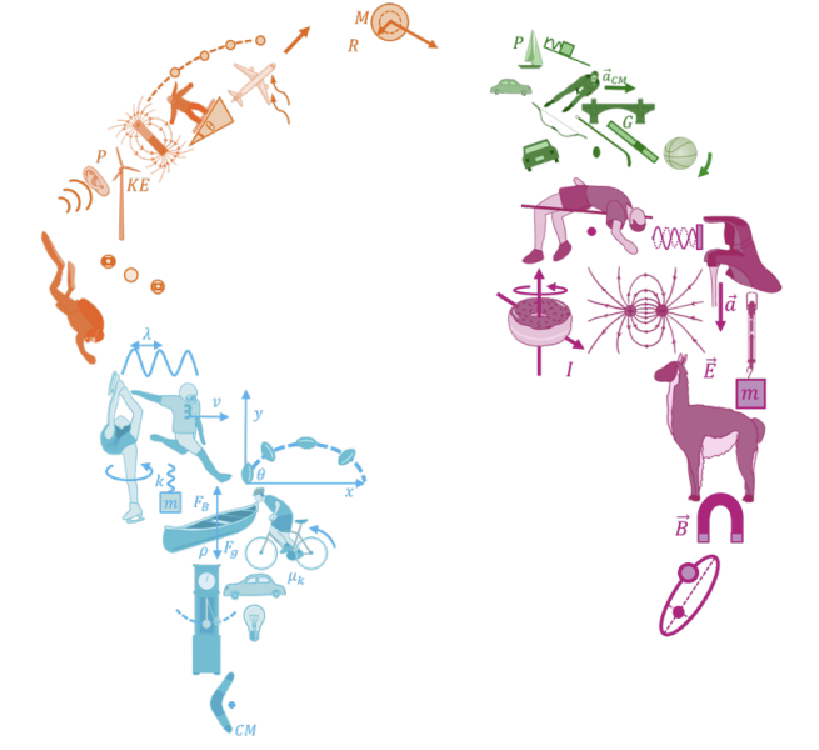
\includegraphics[width=4cm]{figures/BMDW/logo}
\end{textblock*}

\end{frame}

%%%%%%%%%%%%%TOC

\twocolframe{Outline}
{\tableofcontents[sections=28-29, subsectionstyle=show/show]\thispagestyle{empty}}
{\tableofcontents[sections=30, subsectionstyle=show/show]}

%%%%%%%%%%%%%%%%%%%%%%%%%











%%%%%%%%%%%%%%%%%%%%%%%%%%%%%%%%
\section{Angular Quantities and Torque}
\label{sec:angulartquantitesandtorque}
\title{Angular Quantities and Torque}
\institute{Describing Angular Statics and Dynamics}
\author{\insertsubsection}


%%%%%%%%%%%%%%%%%%%%%%%%%
\begin{frame}
\titlepage
\thispagestyle{empty}
\end{frame}

%%%%%%%%%%%%%%%%%%%%%%%%%








%%%%%%%%%%%%%%%%%%%%%%%%%%%%%%%%%%%%%%%%%%%%%%%

\begin{frame}{Context}
We started with $\sum \vec F=m \vec a$, and then:
\begin{itemize}
\item Used $\sum \vec F=m \vec a$ as is.
\item Took $\int (\sum \vec F=m \vec a ) \cdot d\vec l$ to define work and energy.
\item Took $\int (\sum \vec F=m \vec a ) dt$ to introduce impulse and momentum.
\end{itemize}
This week, we do:
\begin{align*}
\vec r \times \Bigl(\sum \vec F=m \vec a \Bigr)
\end{align*}
in order to model rotating systems.
\end{frame}


%%%%%%%%%%%%%%%%%%%%%%%%%%%%%%%%
\subsection{Describing rotating things}
\label{subsec:describingrotatingthings}
\twocolframesf{Describing things that rotate in 2D}
{
\vspace{-0.25cm}
\begin{itemize}
\item Recall that we can describe circular motion using linear or angular quantities:
\begin{align*}
s&=R\theta\\
v&=R\omega\\
a_T&=\alpha R
\end{align*}
\item The angular quantities are \textbf{related to the tangential} linear quantities. The acceleration also has a radial component:
\begin{align*}
a_R=\frac{v^2}{R}=\omega^2 R
\end{align*}
due to the \textbf{change of the direction} of the velocity vector (not its magnitude).
\end{itemize}
}
{
\begin{center}
\begin{tikzpicture}[scale=1]
\tikzmath{
\R=2;
\th=30;
\Px=\R*cos(\th);
\Py=\R*sin(\th);
\vel=1.5;
\vx=-\vel*sin(\th);
\vy=\vel*cos(\th);
}
\scalebox{1}{

\coordinate (P) at (\Px,\Py);

\draw[-latex, line width=1.25pt] (-1.25*\R,0) -- (1.25*\R,0) node[below]{$x$}; 
\draw[-latex, line width=1.25pt] (0,-1.25*\R) -- (0,1.25*\R) node[left]{$y$};

\draw (0,0) circle (\R); 
\fill (P) circle(3pt);
\draw[-latex, line width = 1.5] (0,0) -- (P) node[midway,above] {$\vec r$};
\draw[line width = 1.5] (0.7,0) arc (0:\th:0.7) node[midway,right]{$\theta$};
\draw[-latex, line width = 1.5] (P) -- +(\vx,\vy) node[midway,right=-2pt] {$\vec v$};
\draw[dashed, line width = 1.] (P) -- +(0,\vy) node[midway,right] {$v_y$};
\draw[dashed, line width = 1.] ($(P) +(0,\vy)$) -- +(\vx,0) node[midway,above] {$v_x$};

\draw[dashed] (0,0) --+(225:\R) node[midway,below]{$R$};

\draw[-latex, line width=1] (\R,0) arc (0:\th:\R) node[midway,right]{$s$};

}
\end{tikzpicture}
\captionof*{figure}{\textit{Variables to describe circular motion.}}
\end{center}
}


%%%%%%%%%%%%%%%%%%%%%%%%%%%%%%%%
\twocolframesf{Describing things that rotate in 3D}
{
\begin{itemize}
\item In general, things rotate in a circle:
\begin{itemize}
\item About an axis (defining a normal plane).
\item In a specific direction around the axis.
\item With a specific amplitude/speed/acceleration.
\end{itemize}
\item Use ``axial/pseudo vectors'' to specify:
\begin{itemize}
\item $\vec \theta$, angular displacement.
\item $\vec \omega$, angular velocity.
\item $\vec \alpha$, angular acceleration.
\end{itemize}
with magnitudes given by the same value as in 2D, and \textbf{direction given by the  ``right hand rule for axial vectors''}.
\end{itemize}
}
{
\begin{center}
\begin{tikzpicture}[scale=1]

\scalebox{1}{

\node at (0,0) {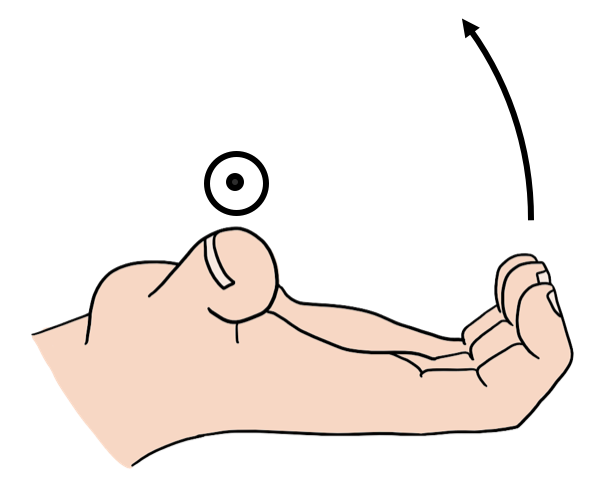
\includegraphics[scale=0.5]{figures/RotationalDynamics/righthandruleaxial}};
\node at (-0.5,1.2) {$\vec \omega$};

}
\end{tikzpicture}
\captionof*{figure}{\textit{The right-hand rule for axial vectors is used to define the direction of a vector associated with rotation. The thumb is parallel to the axis of rotation and the fingers curl in the direction of rotation.}}
\end{center}
}


%%%%%%%%%%%%%%%%%%%%%%%%%%%%%%%%


%%%%%%%%%%%%%%%%%%%%%%%%%%%%%%%%
\subsection{Angular Vectors}
\label{subsec:angularvectors}
\twocolframesf{Angular vectors from linear vectors}
{
\begin{itemize}
\item Need to be able to describe rotation about any axis (not just $x,y,z$).
\item The angular vectors are related to the linear ones:
\begin{align*}
\vec \omega&=\frac{1}{r^2}\vec r \times \vec v\\
\vec \alpha&=\frac{1}{r^2}\vec r \times \vec a
\end{align*}
\item The vector, $\vec r$, is perpendicular to the axis of rotation and goes \textbf{from the axis of rotation to the particle's position}.
\end{itemize}
}
{
\begin{center}
\begin{tikzpicture}[scale=1]
\tikzmath{
\R=1.2;
}

\scalebox{1}{
\begin{scope}[rotate=30]

%angular velocity vector
\draw[-latex, line width=2] (-1,1,0) -- +(0,1,0) node[above]{$\vec \omega$};
%circle around omega
\begin{scope}[canvas is xz plane at y=1.5]
\draw[latex-,dashed] (-1,-0.5) arc(-90:180:0.5);
\end{scope}

\begin{scope}[canvas is xz plane at y=0]
%the plane
\fill[myblue!30] (-1.5*\R,-1.5*\R) -- (1.5*\R,-1.5*\R) -- (1.5*\R,1.5*\R) -- (-1.5*\R,1.5*\R) --cycle;
\draw[line width=1.5,color=myblue!60]  (1.5*\R,-1.5*\R) -- (1.5*\R,1.5*\R)-- (-1.5*\R,1.5*\R);
\draw[line width=1.5] (0,0) circle(\R);
\draw[-latex,line width=1.5,color=myred] (0,0) -- (\R,0) node[midway,above]{\scriptsize $\vec r$};
\draw[-latex,line width=1.5] (\R,0) -- +(0,-1.5) node[midway,right]{\scriptsize $\vec v$};
\end{scope}
\draw[-latex, line width=1] (0,0,0) -- (0,2,0) node[above right] {axis of rotation};
\draw[dotted, line width=1] (0,-0.75,0) -- (0,0,0) ;
\draw[line width=1] (0,-2,0) -- (0,-0.75,0) ;

\end{scope}

}
\end{tikzpicture}
\captionof*{figure}{\textit{An object rotating in a circle in an arbitrary plane. We can define all angular quantities using the linear ones and the vector $\vec r$ from the axis of rotation to the position.}}
\end{center}
}


%%%%%%%%%%%%%%%%%%%%%%%%%%%%%%%%


%%%%%%%%%%%%%%%%%%%%%%%%%%%%%%%%
\subsection{Torque}
\label{subsec:torque}
\begin{frame}{Torque}
\begin{itemize}
\item Recall: A net force exerted on an object causes it to accelerate – forces were introduced as a mathematical quantity to help model the causes of motion.
\begin{align*}
\sum \vec F = m\vec a
\end{align*}
\item Torque is analogous to force, but torques cause an object to have an angular acceleration \textbf{about a specific axis}:
\begin{itemize}
\item A torque is \textbf{only defined relative to a particular axis}.
\item If there is a net torque on an object, it will have an angular acceleration about that axis:
\begin{align*}
\sum \vec \tau=mr^2\vec \alpha
\end{align*}
\end{itemize}
\item[$\rightarrow$]  A larger torque will result in a larger angular acceleration.
\end{itemize}
\end{frame}


%%%%%%%%%%%%%%%%%%%%%%%%%%%%%%%%
\twocolframesf{Torque from a force}
{
\vspace{-0.25cm}
\begin{itemize}
\item Measures how much a force will cause an object to rotate about a given axis (this determines $\vec r$).
\item Defined as:
\begin{align*}
\vec \tau = \vec r \times \vec F
\end{align*} with magnitude:
\begin{align*}
\tau = rF\sin\theta
\end{align*}
\item<2-> The cross product ``picks out'' the components of the vectors that are perpendicular to each other:
\begin{align*}
\tau =r F_\perp = r_\perp F
\end{align*}
\end{itemize}
}
{
\vspace{-1.5cm}
\begin{center}
\begin{tikzpicture}[scale=1]
\tikzmath{
\R=1.2;
\Fl=1.5;
\th=60;
\Flx=\Fl*sin(\th);
\Fly=\Fl*cos(\th);
\rx=\R*sin(\th);
\ry=\R*cos(\th);
}

\scalebox{1}{

\coordinate (P) at (2*\R,0.7*\R);

\fill[myblue!40] (0,0) circle(\R);
\draw[-latex,line width=1.5] (0,0) -- (45:\R) node[midway,above]{\scriptsize $\vec r$}; 
\draw[-latex,line width=1.5,color=myred] (45:\R) -- +(45+\th: \Fl) node[above]{\scriptsize $\vec F$};
\draw[dashed] (45:\R) -- +(45:0.75*\R);
\draw (45:1.2*\R) arc(45:{45+\th}:0.2*\R) node[midway,above]{\scriptsize $\theta$};
\draw[dashed,color=myred,-latex] (45:\R) -- +(135:\Flx) node[midway,above] {\scriptsize $F_\perp$};
\draw[dashed,color=myred,-latex] ($(45:\R)+(135:\Flx)$) -- +(45:\Fly)node[midway,left] {\scriptsize $F_\parallel$};

\fill (P) circle (1pt);
\draw (P) circle (4pt);
\draw[-latex] ($(P)+(-60:0.3)$) arc (-60:60:0.3) node[above] {\scriptsize $\vec \tau = \vec r \times \vec F$};

\only<2>{
\begin{scope}[shift={(\R,-3*\R)}]
\coordinate (P2) at (-2*\R,0.7*\R);
\fill[myblue!40] (0,0) circle(\R);
\draw[-latex,line width=1.5] (0,0) -- (45:\R) node[midway,above]{\scriptsize $\vec r$}; 
\draw[-latex,line width=1.5,color=myred] (45:\R) -- +(45+\th: \Fl) node[above]{\scriptsize $\vec F$};
\draw[dashed] (45:\R) -- +(45:0.75*\R);
\draw (45:1.2*\R) arc(45:{45+\th}:0.2*\R) node[midway,above]{\scriptsize $\theta$};

\draw[dashed,-latex] (0,0) -- +(\th-45:\rx) node[midway,below] {\scriptsize $r_\perp$};
\draw[dashed,-latex] ($(0,0)+(\th-45:\rx)$) -- +(45+\th: \ry) node[midway,right] {\scriptsize $r_\parallel$};


\fill (P2) circle (1pt);
\draw (P2) circle (4pt);
\draw[-latex] ($(P2)+(-60:0.3)$) arc (-60:60:0.3) node[above] {\scriptsize $\vec \tau = \vec r \times \vec F$};
\end{scope}
}
}
\end{tikzpicture}
\captionof*{figure}{\textit{The torque from a force.}}
\end{center}
}


%%%%%%%%%%%%%%%%%%%%%%%%%%%%%%%%
\twocolframesf{Torque to rotate a door}
{
\begin{align*}
\vec \tau &= \vec r \times \vec F\\
\tau &= rF\sin\theta
\end{align*}
\begin{itemize}
\item A given force will result in the largest torque if it is perpendicular to the vector, $\vec r$ ($\sin\theta=1$).
\item A given force will result in the largest torque if the vector, $\vec r$,  has the largest magnitude.
\item That's why the door handles are far from the hinges... You knew this intuitively...
\end{itemize}
}
{
\begin{center}
\begin{tikzpicture}[scale=1]
\tikzmath{
\L=4;
}

\scalebox{1}{

\fill[color=brown!90] (0,-0.1) rectangle (\L,0.1);
\fill (0,0) circle (2pt) node[below]{axis};
\draw[line width = 2] (0.85*\L,-0.1) -- +(0,-0.2) -- +(0.4,-.2);

\draw[latex-, line width=2] (0.5*\L,-0.1) -- +(0,-1) node[below]{$\vec F$};
\draw[latex-, line width=2] (0.75*\L,-0.1) -- +(0,-1) node[below]{$\vec F$};

\draw[-latex] (0,0.2) -- +(0.5*\L,0) node[midway,above]{$\vec r_1$};
\draw[-latex] (0,0.3) -- +(0.75*\L,0) node[midway,above right]{$\vec r_2$};

\draw [-latex, line width =1] (\L,0.3) arc (0:25:\L); 
}
\end{tikzpicture}
\captionof*{figure}{\textit{Rotating a door is easier if you push far away from the hinges, right?}}
\end{center}
}



%%%%%%%%%%%%%%%%%%%%%%%%%%%%%%%%



%%%%%%%%%%%%%%%%%%%%%%%%%%%%%%%%
\section{Angular Dynamics and Moment of Inertia}
\label{sec:angulardynamicsandmomentofinertia}
\title{Angular Dynamics and Moment of Inertia}
\institute{Describing Angular Statics and Dynamics}
\author{\insertsubsection}


%%%%%%%%%%%%%%%%%%%%%%%%%
\begin{frame}
\titlepage
\thispagestyle{empty}
\end{frame}

%%%%%%%%%%%%%%%%%%%%%%%%%





%%%%%%%%%%%%%%%%%%%%%%%%%%%%%%%%
\subsection{Dynamics of rotating objects}
\label{subsec:dynamicsofrotatingobjects}
\begin{frame}{Dynamics of rotating particles}
\begin{itemize}
\item For a point particle:
\begin{align*}
\pvec F^{net} = m\vec a
\end{align*}
\item If we choose an axis of rotation, such that, $\vec r$, is the vector from that axis to the particle:
\begin{align*}
\vec r \times \pvec F^{net} &= m\vec r \times\vec a \quad \quad \text{recall: } \vec \alpha=\frac{1}{r^2}\vec r \times \vec a\\
\therefore \pvec \tau^{net} &= mr^2\vec \alpha
\end{align*}
\item This \textbf{equation only makes sense relative to a specific axis of rotation}. It is valid even if there is nothing actually rotating!
\item The inertia of the particle to rotational motion is given by $mr^2$, and \textbf{depends on both the mass of the particle and its distance to the axis of rotation}.
\item We often refer to this as the rotational version of Newton's Second Law.
\end{itemize}
\end{frame}


%%%%%%%%%%%%%%%%%%%%%%%%%%%%%%%%



%%%%%%%%%%%%%%%%%%%%%%%%%%%%%%%%
\twocolframesf{Dynamics of rotating objects}
{
\begin{itemize}
\item We can extend the description of how one particle rotates about an axis to how a solid object rotates about an axis.
\item An object can be modeled as a ``system'' of particles, each with a torque exerted on it, and a corresponding angular acceleration:
\begin{align*}
\pvec \tau_1^{net} &= m_1r_1^2\vec \alpha_1\\
\pvec \tau_2^{net} &= m_2r_2^2\vec \alpha_2\\
&\dots
\end{align*}
\end{itemize}
}
{
\begin{center}
\begin{tikzpicture}[scale=1]
\tikzmath{
\L=2;
}

\scalebox{1}{

\coordinate (P1) at (1.5,-1);
\coordinate (P2) at (2.5,0);


\draw[line width=1.5] (0,-\L) -- (0,\L) node[above] {axis};

\fill[color=myblue!60] plot [smooth cycle] coordinates {(2,-1.5) (3,0) (1.8,1) (1.5,1.5) (1,1) (0.7,-0.5)};

\fill (P1) circle(2pt) node[above]{$m_1$};
\fill (P2) circle(2pt) node[above]{$m_2$};

\draw[latex-, line width=1.5] (P2) -- (0,0) node[midway,above]{$\vec r_2$};
\draw[latex-, line width=1.5] (P1) -- (0,-1) node[midway,below]{$\vec r_1$};

\draw[-latex, line width=1] (-1.5,0.95*\L) arc(-180:45:1.5 and 0.3);

}
\end{tikzpicture}
\captionof*{figure}{\textit{Two particles in a solid object rotating about an axis.}}
\end{center}
}


%%%%%%%%%%%%%%%%%%%%%%%%%%%%%%%%



%%%%%%%%%%%%%%%%%%%%%%%%%%%%%%%%
\twocolframesf{Dynamics of rotating objects}
{
\begin{itemize}
\item Rotational version of Newton’s Second Law true for each particle:
\begin{align*}
\pvec \tau_1^{net} &= m_1r_1^2\vec \alpha_1\\
\pvec \tau_2^{net} &= m_2r_2^2\vec \alpha_2\\
&\dots
\end{align*}
\item Sum these all together:
\begin{itemize}
\item \textbf{All particles have the same angular acceleration}.
\item When summing the torques on each particle, all of the internal torques (due to internal forces) cancel:
\begin{align*}
\sum \pvec \tau^{ext}=\left(\sum m_ir_i^2  \right)\vec \alpha
\end{align*}
\end{itemize}

\end{itemize}
}
{
\begin{center}
\begin{tikzpicture}[scale=1]
\tikzmath{
\L=2;
}

\scalebox{1}{

\coordinate (P1) at (1.5,-1);
\coordinate (P2) at (2.5,0);


\draw[line width=1.5] (0,-\L) -- (0,\L) node[above] {axis};

\fill[color=myblue!60] plot [smooth cycle] coordinates {(2,-1.5) (3,0) (1.8,1) (1.5,1.5) (1,1) (0.7,-0.5)};

\fill (P1) circle(2pt) node[above]{$m_1$};
\fill (P2) circle(2pt) node[above]{$m_2$};

\draw[latex-, line width=1.5] (P2) -- (0,0) node[midway,above]{$\vec r_2$};
\draw[latex-, line width=1.5] (P1) -- (0,-1) node[midway,below]{$\vec r_1$};

\draw[-latex, line width=1] (-1.5,0.95*\L) arc(-180:45:1.5 and 0.3);

}
\end{tikzpicture}
\captionof*{figure}{\textit{The particles in a solid object rotating about an axis all have the same angular acceleration relative to that axis.}}
\end{center}
}


%%%%%%%%%%%%%%%%%%%%%%%%%%%%%%%%
\subsection{Moment of inertia}
\label{subsec:momentofinertia}
\begin{frame}{The moment of inertia}
\begin{itemize}
\item The net external torque on an object determines its angular acceleration:
\begin{align*}
\sum \pvec \tau^{ext}=\left(\sum m_ir_i^2  \right)\vec \alpha
\end{align*}
\item We introduce, $I$, the ``moment of inertia'' of an object \textbf{relative to a given axis of rotation}:
\begin{align*}
I=\sum m_ir_i^2  
\end{align*}
\item Rotational version of Newton's Second Law:
\begin{align*}
\sum \pvec \tau^{ext}=I\vec \alpha
\end{align*}
\item Instead of force, we have torque, instead of mass, we have moment of inertia, instead of linear acceleration, we have angular acceleration.
\end{itemize}
\end{frame}


%%%%%%%%%%%%%%%%%%%%%%%%%%%%%%%%
\begin{frame}{Rotational vs Linear dynamics}
\begin{itemize}
\item Recall, for an object, the \textbf{net external force} on the object determines \textbf{the acceleration of the CM}:
\begin{align*}
\sum \pvec F^{ext}=M\vec a_{CM}
\end{align*}
\item Similarly, the \textbf{net external torque} about an axis on the object determines its \textbf{angular acceleration} relative to that axis:
\begin{align*}
\text{cause of motion}\quad\quad\sum \pvec \tau^{ext}=I\vec \alpha\quad\quad\text{(resistance to motion)(kinematic quantity)}
\end{align*}
\item The moment of inertia has a similar ``role'' as the mass in Newton's Second Law. For a given torque, the object with the smaller moment of inertia will have the largest angular acceleration.
\end{itemize}
\end{frame}



%%%%%%%%%%%%%%%%%%%%%%%%%%%%%%%%
\subsection{Group exercise: moment of inertia for a 2 mass system}
\label{subsec:}
\twocolframesf{Group exercise}
{
\begin{itemize}
\item Calculate the moment of inertia for a system of 2 masses connected by a mass-less rod of length $d$, for:
\begin{itemize}
\item An axis that goes through $m_1$.
\item An axis that goes through 0 ($d$ away from $m_1$).
In both cases, the axis is perpendicular to the page.
\end{itemize}
\begin{align*}
I=\sum m_ir_i^2  
\end{align*}
\item<2> Applying the formula:
\begin{align*}
I_{m_1}&=m_1(0)^2+m_2d^2=m_2d^2\\
I_{0}&=m_1(d)^2+m_2(2d)^2=(m_1+4m_2)d^2\\
\end{align*}
\end{itemize}
}
{
\begin{center}
\begin{tikzpicture}[scale=1]
\tikzmath{
\d=1.5;
}

\scalebox{1}{

\fill (0,0) circle (1pt) node[right] {0};
\fill (0,\d) circle (2pt) node[right=5pt] {$m_1$};
\fill (0,2*\d) circle (2pt) node[right=5pt] {$m_2$};
\draw[latex-latex] (-0.2,0) -- +(0,\d) node[midway, left]{$d$};
\draw[latex-latex] (-0.2,\d) -- +(0,\d) node[midway, left]{$d$};
\draw[line width=1] (0,\d) -- +(0,\d);
}
\end{tikzpicture}
\captionof*{figure}{\textit{Two masses connected by a mass-less rods rotate around an axis perpendicular to the page.}}
\end{center}
}


%%%%%%%%%%%%%%%%%%%%%%%%%%%%%%%%



%%%%%%%%%%%%%%%%%%%%%%%%%%%%%%%%
\subsection{Formula}
\label{subsec:iformula}
\begin{frame}{Calculating moment of inertia}
\begin{itemize}
\item Similar to centre of mass, which is a mass-weighted sum of the position coordinate:
\begin{align*}
x_{CM}=\frac{1}{M}\sum m_ix_i=\frac{1}{M}\int_0^M xdm
\end{align*}
\item For the moment of inertia, it is a mass-weighted sum of the \textbf{distance to the axis of rotation squared}:
\begin{align*}
I=\sum m_ir_i^2  =\int_0^M r^2 dm
\end{align*}
\end{itemize}
\end{frame}


%%%%%%%%%%%%%%%%%%%%%%%%%%%%%%%%
\subsection{Example: moment of inertia of a rod about its end}
\label{subsec:}
\twocolframesf{Continuous objects: Moment of inertia of a rod about its end}
{
\begin{itemize}
\item Define mass per unit length: $\lambda =\frac{M}{L}$
\item Choose a mass element on the rod, $dm$, of length, $dr$ , at a distance, $r$, from the axis of rotation, it has mass:
\begin{align*}
dm=\lambda dr
\end{align*}
\item The total moment of inertia is the sum over all mass elements:
\begin{align*}
I_{end}&=\sum m_ir_i^2  =\int_0^M r^2 dm = \int_0^L \lambda r^2 dr\\
&=\lambda \frac{1}{3}L^3=\frac{1}{3}ML^2
\end{align*}
\end{itemize}
}
{
\begin{center}
\begin{tikzpicture}
\tikzmath{
\L=5;
\n=15;
}
\scalebox{1}{

\draw[-latex,line width=1] (0,0) -- (\L,0) node[below]{$r$};
\draw (0,0.1) -- +(0,-0.2) node[below]{0} node[below=10pt]{(axis)};
\draw (\L/\n*13,0.1) -- +(0,-0.2) node[below]{$L$};


\foreach \i in {1,...,13}{
\tikzmath{
\dx=\L/\n;
\xxi=\dx*(\i-1);
}
\draw (\xxi,0.5) rectangle (\xxi+\dx,0.75);
\ifthenelse{\i=7}{
\fill[color=myblue!60] (\xxi,0.5) rectangle (\xxi+\dx,0.75);
\node at (\xxi+0.5*\dx,1) {\scriptsize $dm$};
\draw (\xxi+0.5*\dx,0.1) -- +(0,-0.2) node[below]{$r$};
}{}

\ifthenelse{\i=2}{
\draw[latex-latex] (\xxi,0.9) -- +(0\dx,0) node[midway,above]{\scriptsize $dr$};
}{}

}


}
\end{tikzpicture}
\captionof*{figure}{\textit{To find the moment of inertia of a one dimensional object, model it as being made of many \textit{point} masses, $dm$, each with an infinitesimal length, $dx$.}}
\end{center}
}


%%%%%%%%%%%%%%%%%%%%%%%%%%%%%%%%
\begin{frame}{Group exercise}
Determine the moment of inertia of a uniform rod about is centre of mass:
\begin{itemize}
\item Do you expect it to be bigger or smaller than moment of inertia about its end?
\end{itemize}
\end{frame}


%%%%%%%%%%%%%%%%%%%%%%%%%%%%%%%%
\twocolframesf{Continuous objects: Moment of inertia of a rod about its end}
{
\begin{itemize}
\item Define mass per unit length: $\lambda =\frac{M}{L}$
\item Choose a mass element on the rod, $dm$, of length, $dr$ , at a distance, $r$, from the axis of rotation, it has mass:
\begin{align*}
dm=\lambda dr
\end{align*}
\item The total moment of inertia is the sum over all mass elements:
\begin{align*}
I_{CM}&=\sum m_ir_i^2  =\int_0^M r^2 dm = \int_{\textcolor{myred}{-\frac{L}{2}}}^{\textcolor{myred}{+\frac{L}{2}}} \lambda r^2 dr\\
&=\lambda \left[\frac{1}{3}r^3\right]_{\textcolor{myred}{-\frac{L}{2}}}^{\textcolor{myred}{+\frac{L}{2}}} =\frac{1}{12}\lambda ML^3=\frac{1}{12}ML^2
\end{align*}
\end{itemize}
}
{
\vspace{-0.5cm}
\begin{center}
\begin{tikzpicture}
\tikzmath{
\L=5;
\n=15;
}
\scalebox{1}{

\draw (0,0.1) -- +(0,-0.2) node[below]{$-\frac{L}{2}$};
\draw[-latex,line width=1] (0,0) -- (\L,0) node[below]{$r$};
\draw (\L/\n*13,0.1) -- +(0,-0.2) node[below]{$\frac{L}{2}$};


\foreach \i in {1,...,13}{
\tikzmath{
\dx=\L/\n;
\xxi=\dx*(\i-1);
}
\draw (\xxi,0.5) rectangle (\xxi+\dx,0.75);
\ifthenelse{\i=7}{
\fill[color=myblue!60] (\xxi,0.5) rectangle (\xxi+\dx,0.75);
\node at (\xxi+0.5*\dx,1) {\scriptsize $dm$};
%\draw (\xxi+0.5*\dx,0.1) -- +(0,-0.2) node[below]{$r$};
\draw (\xxi+0.5*\dx,0.1) -- +(0,-0.2) node[below]{0} node[below=10pt]{(axis)};
}{}

\ifthenelse{\i=2}{
\draw[latex-latex] (\xxi,0.9) -- +(0\dx,0) node[midway,above]{\scriptsize $dr$};
}{}

}


}
\end{tikzpicture}
\captionof*{figure}{\textit{To find the moment of inertia of a rod about CM, we move the origin to the axis of rotation, so that $r$ measures distance to the axis.}}
\end{center}
Alternatively, we could have added the moment of inertia of two rods of length $\frac{1}{2}L$ (and mass $\frac{M}{2}$) rotated about their ends:
\begin{align*}
I_{CM}&=2\frac{1}{3}\frac{M}{2}\left(\frac{L}{2} \right)^2=\frac{1}{12}ML^2
\end{align*}
}



%%%%%%%%%%%%%%%%%%%%%%%%%%%%%%%%
\subsection{Parallel axis theorem}
\label{subsec:parallelaxistheorem}
\twocolframesf{Parallel axis theorem}
{
\begin{itemize}
\item Given the moment of inertia about an axis that goes through the CM, the moment of inertia about an axis that is parallel and goes through a different point, a distance, $h$ away is given by:
\begin{align*}
I_h=I_{CM}+Mh^2
\end{align*}
\item For a rod, find the moment of inertia about the CM, given the moment of inertia about one end:
\begin{align*}
I_{end}&=\frac{1}{3}ML^2\\
I_{CM}&=I_{end}-M\left(\frac{L}{2}\right)^2=\frac{1}{3}ML^2-\frac{1}{4}ML^2=\frac{1}{12}ML^2
\end{align*}
\end{itemize}
}
{
\vspace{-0.5cm}
\begin{center}
\begin{tikzpicture}
\tikzmath{
\R=1;
\h=2;
\L=4;
}
\scalebox{1}{

\node at (-0.75*\R,0.5*\R){$M$};
\fill[color=myblue!60] circle ({\R} and {\R/4});
\draw[line width=1] (0,0) -- +(0,0.75*\L/2);
\draw[line width=1] (0,-0.75*\L/2) -- (0,-\R/4);
\draw[line width=1, dotted] (0,-\R/4) -- (0,0);
\fill[color=myblue!80] (\R,0) arc(0:-180:{\R} and {\R/4}) -- (-\R,-0.2) arc(180:360:{\R} and {\R/4}) -- cycle;

\draw[line width=1.5] (\h,-\L/2) -- +(0,\L)node[above]{axis};
\draw[latex-latex] (0,\L/4) -- +(\h,0)node[midway,above]{$h$} ;

\draw[-latex,line width=1] (0,\L/2) arc(180:390:{\h} and {\h/4});

}
\end{tikzpicture}
\captionof*{figure}{\textit{The moment of inertia of an object about an axis a distance, $h$, away from the CM is given by the parallel axis theorem.}}
\end{center}

}

%%%%%%%%%%%%%%%%%%%%%%%%%%%%%%%%

%%%%%%%%%%%%%%%%%%%%%%%%%%%%%%%%%%%%%%

\begin{frame}{Quick review}
\subsection{Review}
\label{subsec:review}
\begin{itemize}
\item Torque from a force \textbf{about an axis}:
\begin{align*}
\vec \tau =\vec r \times \vec F
\end{align*}
\item Rotational equivalent of Newton's Second Law:
\begin{align*}
\pvec \tau^{net}&=mr^2\vec \alpha\quad \text{(particle)}\\
\sum \pvec \tau^{ext}&=I\vec \alpha\quad \text{(object)}
\end{align*}
\item Moment of inertia of an object \textbf{about an axis}:
\begin{align*}
I=\sum m_ir_i^2  =\int_0^M r^2 dm
\end{align*}
\item Parallel axis theorem:
\begin{align*}
I_h=I_{CM}+Mh^2
\end{align*}
\end{itemize}
\end{frame}

%%%%%%%%%%%%%%%%%%%%%%%%%%








%%%%%%%%%%%%%%%%%%%%%%%%%%%%%%%%
\section{Equilibriem with Rotational Dynamics}
\label{sec:equilibirem}
\title{Equilibriem with Rotational Dynamics}
\institute{Describing Angular Statics and Dynamics}
\author{\insertsubsection}


%%%%%%%%%%%%%%%%%%%%%%%%%
\begin{frame}
\titlepage
\thispagestyle{empty}
\end{frame}

%%%%%%%%%%%%%%%%%%%%%%%%%





%%%%%%%%%%%%%%%%%%%%%%%%%%%%%%%%
\subsection{Concept}
\label{subsec:concept}
\twocolframe{Equilibrium}
{
\begin{itemize}
\item Just because the sum of the external forces on an object is zero does not mean that the object does not move. It only means that the centre of mass does not accelerate:
\begin{align*}
\sum \pvec F^{ext}=m\vec a_{CM}
\end{align*}
\item For the object to be ``in equilibrium'' the sum of the torques on the object must also be zero:
\begin{align*}
\sum \pvec \tau^{ext}=I\vec \alpha
\end{align*}
\end{itemize}

}
{
\begin{center}
\begin{tikzpicture}[scale=1]
\tikzmath{
\L=2;
}

\scalebox{1}{
\fill[color=myblue!80] (-\L,-0.1) rectangle (\L,0.1);
\draw[latex-,line width=1] (-0.75*\L,-0.1) -- +(0,-1) node[midway,right] {$\vec F$};
\draw[latex-,line width=1] (0.75*\L,0.1) -- +(0,1) node[midway,left] {$-\vec F$};
}
\end{tikzpicture}
\captionof*{figure}{\textit{The net force on this bar is zero, but it will rotate because the net torque (about any axis!) is not zero. }}
\end{center}
}


%%%%%%%%%%%%%%%%%%%%%%%%%%%%%%%%


%%%%%%%%%%%%%%%%%%%%%%%%%%%%%%%%

%%%%%%%%%%%%%%%%%%%%%%%%%%%%%%%%
\twocolframe{Equilibrium}
{
\begin{itemize}
\item Just because the sum of the external forces on an object is zero does not mean that the object does not move. It only means that the centre of mass does not accelerate:
\begin{align*}
\sum \pvec F^{ext}=m\vec a_{CM}
\end{align*}
\item For the object to be ``in equilibrium'' the sum of the torques \textcolor{myred}{about any axis} on the object must also be zero:
\begin{align*}
\sum \pvec \tau^{ext}=I\vec \alpha
\end{align*}
\end{itemize}

}
{
\begin{center}
\begin{tikzpicture}[scale=1]
\tikzmath{
\L=2;
}

\scalebox{1}{
\fill[color=myblue!80] (-\L,-0.1) rectangle (\L,0.1);
\draw[latex-,line width=1] (-0.75*\L,-0.1) -- +(0,-1) node[midway,right] {$\vec F$};
\draw[latex-,line width=1] (0.75*\L,0.1) -- +(0,1) node[midway,left] {$-\vec F$};
}
\end{tikzpicture}
\captionof*{figure}{\textit{The net force on this bar is zero, but it will rotate because the net torque is not zero. Note that it will rotate about the CM because that is the point that behaves according to the net external force, which is zero, so the CM does not move!}}
\end{center}
}


%%%%%%%%%%%%%%%%%%%%%%%%%%%%%%%%



%%%%%%%%%%%%%%%%%%%%%%%%%%%%%%%%
\subsection{Example: ladder}
\label{subsec:exampleladder}
\twocolframesf{Example: ladder}
{
\only<1>{
\begin{itemize}
\item Group question: Draw the forces on the ladder.
\end{itemize}
}
\only<2>{
\begin{itemize}
\item The friction force on the ground prevents the bottom of the ladder from sliding away.
\item If you consider the torques about the contact point with the ground, the torque on the ladder from the weight of the person on the ladder gets bigger as they climb up:
\begin{itemize}
\item Only $R$ can grow and exert a torque in the opposite direction to keep the ladder in equilibrium.
\item As $R$ increases, $f_s$ must also increase (not net force in the horizontal direction).
\end{itemize}
\item When someone ``spots you'' on a ladder, the most important is that they prevent the bottom of the ladder from sliding away from the wall.

\end{itemize}
}
}
{
\begin{center}
\begin{tikzpicture}[scale=1]
\tikzmath{
\L=5;
\abox=0.5;
\th=60;
\xl=0.5*\L;
\ladl=\xl/cos(\th);
}

\scalebox{1}{
\coordinate (P) at (-\xl,0);
\coordinate (R) at ($(P)+(\th:\ladl)$);
\coordinate (B) at ($(P)+(\th:0.75*\ladl)$);

\fill (-0.75*\L,-0.2) rectangle (0,0);
\fill (0,-0.2) rectangle (0.2,1*\L);

\draw[line width=2,color=brown] (P) -- (R);
\draw ($(P)+(0.5,0)$) arc(0:\th:0.5) node[midway,right]{$\theta$};

\begin{scope}[rotate=\th]
\fill[color=myblue!80] (B) -- ($(B)+(0:\abox)$) -- ($(B)+(0:\abox)+(90:\abox)$)-- ($(B)+(90:\abox)$) -- cycle;
\end{scope}

\only<2>{
\draw[-latex,color=red,line width=2] (P) -- +(0,2) node[midway,left]{$\vec N$};
\draw[-latex,color=red,line width=2] (P) -- +(1,0) node[midway,below]{$\vec f_s$};

\draw[-latex,color=red,line width=2] ($(P) +(\th:0.5*\ladl)$) -- +(0,-1)node[right]{$M\vec g$};
\draw[-latex,color=red,line width=2] ($(P) +(\th:0.75*\ladl+\abox/2)$) -- +(0,-1)node[below]{$m\vec g$};

\draw[-latex,color=red,line width=2] (R) -- +(-1,0) node[midway,above]{$\vec R$};


}

}
\end{tikzpicture}
\only<1>{\captionof*{figure}{\textit{A ladder with a weight on it.}}}
\only<2>{\captionof*{figure}{\textit{Forces exerted \textbf{on the ladder}.}}}
\end{center}
}


%%%%%%%%%%%%%%%%%%%%%%%%%%%%%%%%


%%%%%%%%%%%%%%%%%%%%%%%%%%%%%%%%
\subsection{CM of irregular shapes}
\label{subsec:cmofirregularshapes}
\twocolframe{Example: Find CM of object}
{
\begin{itemize}
\item Only two forces on the object:
\begin{itemize}
\item Weight \textbf{exerted at the CM}.
\item Normal force exerted by the pin.
\end{itemize}
\item Since the object is in equilibrium, there is no net torque.
\item The CM must be located exactly below the pin, or the weight and normal force would create a net torque.
\end{itemize}
}
{
\begin{center}
\begin{tikzpicture}[scale=1]
\tikzmath{
\th=80;
\L=1.2;
}

\scalebox{1}{

\coordinate (CM) at (0,0);

\fill[color=myblue!40] ($(CM)+(80:0.8*\L)$) -- ($(CM)+(30:\L)$) -- ($(CM)+(-45:\L)$)  -- ($(CM)+(-80:0.6*\L)$) -- ($(CM)+(250:1.1*\L)$) -- ($(CM)+(225:1.3*\L)$) -- ($(CM)+(180:1.1*\L)$) -- ($(CM)+(120:0.7*\L)$) -- cycle;

\fill ($(CM)+(0,0.6*\L)$) circle(2pt);
\fill[color=red] ($(CM)+(10:0.6*\L)$) circle(2pt);
\draw[-latex,line width=2] ($(CM)+(0,0.6*\L)$) --+(0,1) node[left]{$\vec N$};
\draw[dashed] ($(CM)+(0,0.6*\L)$) --+(0,-2);
\draw[-latex,line width=2] ($(CM)$) --+(0,-1) node[right]{$\vec F_g$};
\node at (CM) {$\times$};
\node[left] at (CM) {\scriptsize CM};


\begin{scope}[shift={(2.5*\L,0)}]

\coordinate (CM) at (0,0);
\begin{scope}[rotate=\th]
\fill[color=myblue!40] ($(CM)+(80:0.8*\L)$) -- ($(CM)+(30:\L)$) -- ($(CM)+(-45:\L)$)  -- ($(CM)+(-80:0.6*\L)$) -- ($(CM)+(250:1.1*\L)$) -- ($(CM)+(225:1.3*\L)$) -- ($(CM)+(180:1.1*\L)$) -- ($(CM)+(120:0.7*\L)$) -- cycle;
\fill ($(CM)+(0,0.6*\L)$) circle(2pt);
\end{scope}


\fill[color=red] ($(CM)+(\th+10:0.6*\L)$) circle(2pt);
\draw[-latex,line width=2] ($(CM)+(10+\th:0.6*\L)$) --+(0,1) node[left]{$\vec N$};
\draw[dashed] ($(CM)+(10+\th:0.6*\L)$) --+(0,-2);
\draw[-latex,line width=2] ($(CM)$) --+(0,-1) node[right]{$\vec F_g$};
\node at (CM) {$\times$};
\node[left] at (CM) {\scriptsize CM};

\end{scope}

}
\end{tikzpicture}
\captionof*{figure}{\textit{Rotating a 2D shape and using a plumbline to find its CM. The CM corresponds to the location where the net force of gravity is exerted, sometimes called the ``centre of gravity''.}}
\end{center}
}


%%%%%%%%%%%%%%%%%%%%%%%%%%%%%%%%



%%%%%%%%%%%%%%%%%%%%%%%%%%%%%%%%
\subsection{Dynamics cs static equilibriem}
\label{subsec:dynamicsvsstaticequilibriem}
\begin{frame}{Dynamic vs Static equilibrium}
\begin{itemize}
\item Equilibrium $\rightarrow$ Sum of the torques is zero.
\item Static equilibrium $\rightarrow$ The net force is zero (the CM does not accelerate).
\item Dynamic equilibrium $\rightarrow$ The net force is not zero (the CM accelerates, as does any axis of rotation that is ``attached'' to the object).
\end{itemize}
\end{frame}


%%%%%%%%%%%%%%%%%%%%%%%%%%%%%%%%
\subsection{Speed skater example}
\label{subsec:speed skater example}
\twocolframe{Speed skater in dynamic equilibrium}
{
\only<1>{
\begin{itemize}
\item The skater is accelerating to the left (going around a curve, centre of the circle is to the left).
\item The skater is \textbf{not} rotating about her CM!
\begin{itemize}
\item The torques from the normal force and the friction force cancel.
\end{itemize}
\item However, taking the torques about the bottom point, we find there is a net torque from gravity. What is going on?
\end{itemize}

}
\only<2>{
\begin{itemize}
\item The sum of torques about the bottom point is not zero! Why?
\begin{itemize}
\item The accelerating skater is a \textbf{non-inertial frame of reference}. The \textbf{bottom point corresponds to an axis that is accelerating} with the skater.
\item You can take the torques about the bottom point if you consider \textbf{inertial forces}.
\item You \textbf{can always take the torques about the CM}, because the inertial force exerted at the CM will result in no torque, so it won’t matter if the CM is accelerating.
\end{itemize}
\end{itemize}
}
}
{
\vspace{-0.75cm}
\begin{center}
\begin{tikzpicture}[scale=1]
\tikzmath{
\h=2.5;
\L=3;
}

\scalebox{1}{
\node at (0,\h){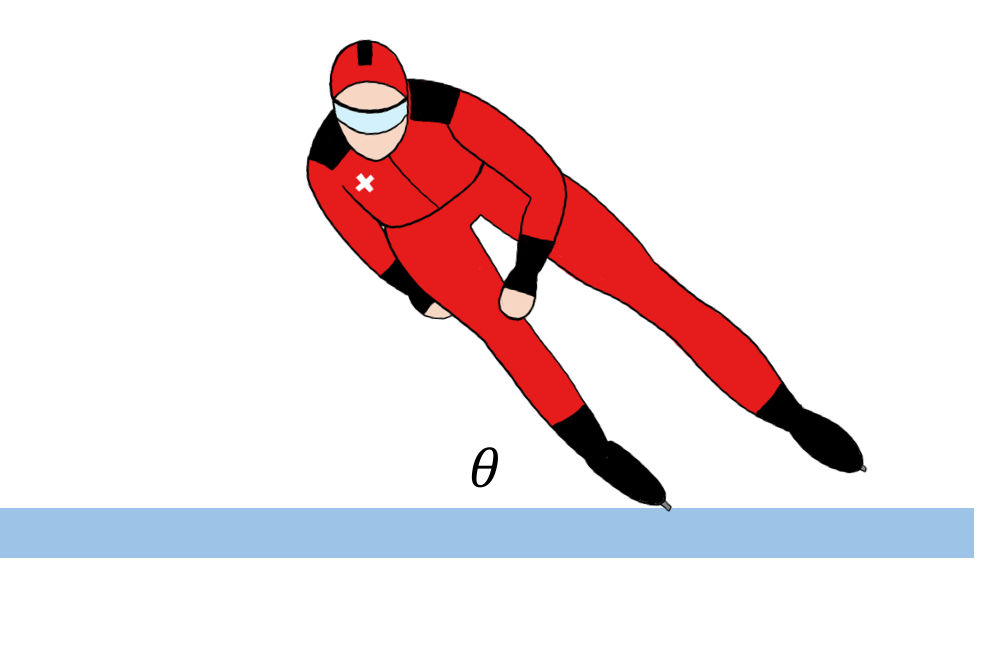
\includegraphics[scale=0.3]{figures/RotationalDynamics/skater}};

\draw [line width=3,color=red] (135:\L/2) -- (-45:\L/2);
\fill (0,0) circle (2pt) node[below left]{\scriptsize CM};
\draw [-latex,line width=2] (0,0) -- +(0,-1) node[left]{$\vec F_g$};
\draw [-latex,line width=2] (-45:\L/2) -- +(0,1) node[right]{$\vec N$};
\draw [-latex,line width=2] (-45:\L/2) -- +(-0.75,0) node[below]{$\vec f_s$};
\only<1>{
\draw [-latex,line width=3] (-0.3*\L,0) -- +(-1,0) node[below]{$\vec a_{CM}$};
}
\only<2>{
\draw [-latex,line width=2] (0,0) -- +(0.75,0) node[above]{$-m\vec a_{CM}$};
}
}
\end{tikzpicture}
\only<1>{\captionof*{figure}{\textit{Forces on a speed skater, as viewed from the ground.}}}
\only<2>{\captionof*{figure}{\textit{Forces on a speed skater, as viewed from a reference frame accelerating with the skater. You need to include inertial forces if taking torques in an accelerating frame of reference!}}}
\end{center}
}


%%%%%%%%%%%%%%%%%%%%%%%%%%%%%%%%


%%%%%%%%%%%%%%%%%%%%%%%%%%%%%%%%
\subsection{Car going around a curve}
\label{subsec:cargoingaroundacurve}
\twocolframesf{Car going around a curve}
{
\begin{itemize}
\item The friction forces, $\vec f_s$, from the tires, perpendicular to the direction of motion, provide the ``centripetal force'' (the net force towards the centre of the circle).
\item These create a net torque about the CM of the car.
\item The car leans to the left (and compresses the shocks which provide the counter torque).
\end{itemize}
}
{
\begin{center}
\begin{tikzpicture}[scale=1]
\tikzmath{
\L=4;
\h=3;
}

\scalebox{1}{
\node at (0,\h) {
\includegraphics[scale=1.2]{figures/RotationalDynamics/car}};
\draw[-latex, line width=1.5] (0.85,0.77*\h) -- +(1,0) node[below]{$\vec f_{s1}$};
\draw[-latex, line width=1.5] (-0.98,0.77*\h) -- +(1.2,0) node[below]{$\vec f_{s2}$};
\draw[-latex, line width=3] (1.2,1*\h) -- +(1.5,0) node[midway,above]{$\vec a_{CM}$};

\node at (0,0) {\animategraphics[autoplay,loop,width=4cm]{10}{figures/RotationalDynamics/cornering}{1}{19}};
}
\end{tikzpicture}
\captionof*{figure}{\textit{https://www.youtube.com/watch?v=Uqr6TpMrfmg}}
\end{center}
}

%%%%%%%%%%%%%%%%%%%%%%%%%%%%%%%%
\subsection{Braking}
\label{subsec:braking}
\begin{frame}{Braking}
\vspace{-1cm}
\begin{center}
\begin{tikzpicture}[scale=1]
\tikzmath{
}

\scalebox{1}{
\node at (0,0) {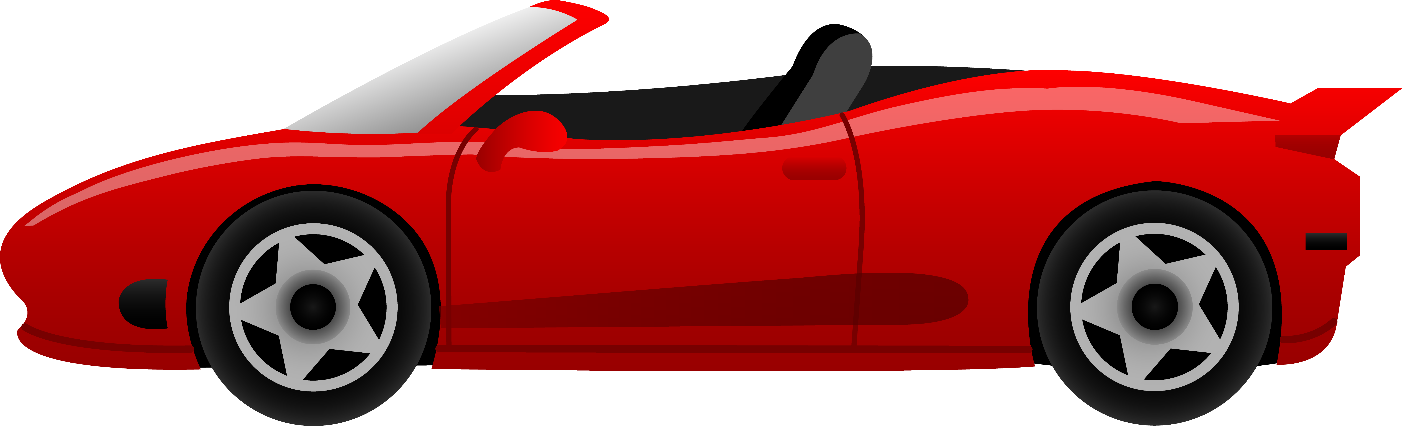
\includegraphics[scale=0.4]{figures/RotationalDynamics/racecar}};
\draw[-latex, line width=1.5] (2.1,-0.97) -- +(1,0) node[below]{$\vec f_{s1}$};
\draw[-latex, line width=1.5] (-1.8,-0.97) -- +(2,0) node[below]{$\vec f_{s2}$};

\node at (6.5,1.75) {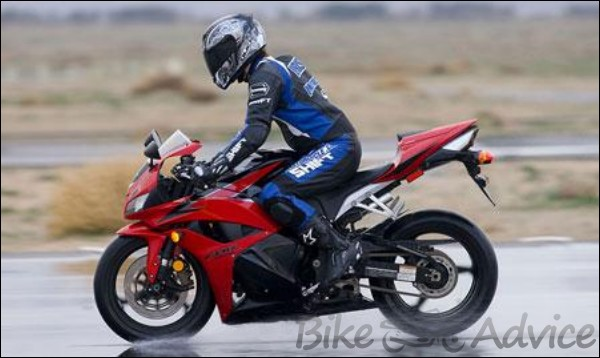
\includegraphics[scale=0.7]{figures/RotationalDynamics/bike}};
\node at (10,1.75) {\tiny{Brissette, P. (2012, April 1). 2009}};
\node at (10,1.5) {\tiny{Honda CBR600RR C-ABS review}};
\node at (9.5,1.25) {\tiny{Motorcycle.com.}};
\node at (6.5,-0.65) {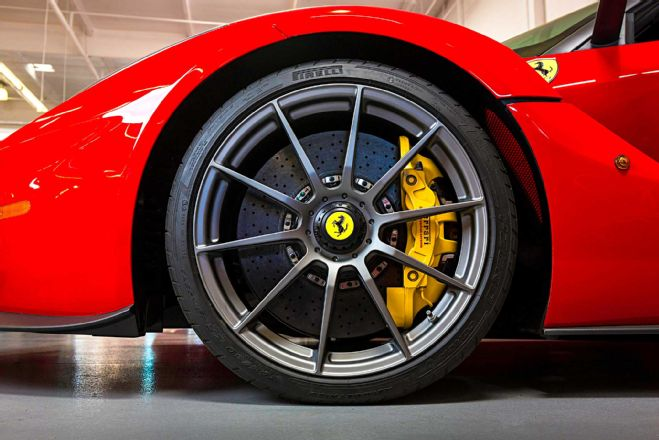
\includegraphics[scale=0.15]{figures/RotationalDynamics/ferrari}};
\node at (9.65,-0.65) {\tiny{2018 812 superfast for sale in}};
\node at (9.1,-0.90) {\tiny{Le Mans France}};
\node at (9.3,-1.15) {\tiny{preowned.ferrari.com}};
}
\end{tikzpicture}
\captionof*{figure}{\textit{Due to the torque from the braking wheels and resulting normal force, the front wheel(s) do most of the braking}}
\end{center}


\begin{itemize}
\item The friction forces from the tires provide the force to decelerate.
\item The front of the car goes down because of the net torque about the CM of the car.
\item The normal force is greater at the front, the front wheels do most of the breaking! Look at the breaks in a car/motorcycle: they are \textit{way} bigger on the front wheels!
\end{itemize}
\end{frame}

%%%%%%%%%%%%%%%%%%%%%%%%%%%%%%%%





























%%%%%%%%%%%%%%%%%%%%%%%%%%%%%%%%

\title{Angular Momentum and Rolling}
\subject{Rotational Energy, Momentum and RWS}
\subtitle{Building Models to Describe our World}




%%%%%%%%%%%%%%%%%%%%%%%%%
%%%%%% Title slide %%%%%%
%%%%%%%%%%%%%%%%%%%%%%%%%
\chaptertitle{Angular Momentum and Rolling}
\begin{frame}
\label{chap:angularmomentumrolling}
\titlepage
\thispagestyle{empty}

\begin{textblock*}{5cm}(11cm,4cm)
    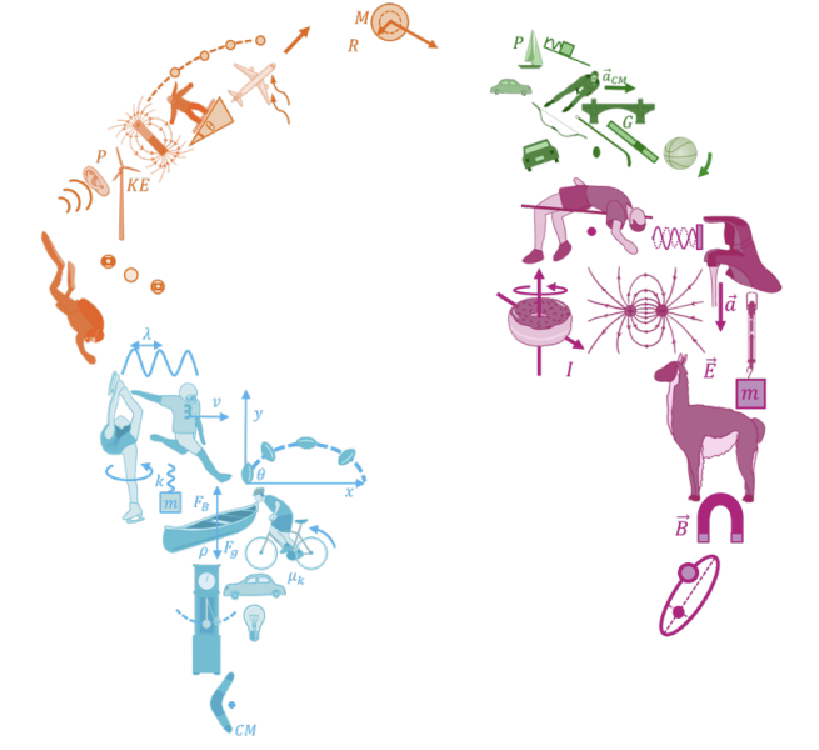
\includegraphics[width=4cm]{figures/BMDW/logo}
\end{textblock*}

\end{frame}

%%%%%%%%%%%%%TOC

\twocolframe{Outline}
{\tableofcontents[sections=31-32, subsectionstyle=show/show]\thispagestyle{empty}}
{\tableofcontents[sections=33, subsectionstyle=show/show]}

%%%%%%%%%%%%%%%%%%%%%%%%%











%%%%%%%%%%%%%%%%%%%%%%%%%%%%%%%%
\section{Angular and Rolling Motion}
\label{sec:angularandrollingmotion}
\title{Angular and Rolling Motion}
\institute{Rotational Energy, Momentum and RWS}
\author{\insertsubsection}


%%%%%%%%%%%%%%%%%%%%%%%%%
\begin{frame}
\titlepage
\thispagestyle{empty}
\end{frame}

%%%%%%%%%%%%%%%%%%%%%









\subsection{Review: Rotational Dynamics}
\label{subsec:rotationaldynamicsreview}
\twocolframe{Quick review: Rotational dynamics}
{
\begin{itemize}
\item Torque on a body \textbf{about an axis}:
\begin{align*}
\vec \tau = \vec r \times \vec F
\end{align*}
\item Rotational equivalent of Newton's Second Law:
\begin{align*}
\sum \pvec \tau^{ext}=I\vec \alpha
\end{align*}
\item Moment of inertia of an object \textbf{about an axis}:
\begin{align*}
I = \sum m_ir_i^2=\int_0^Mr^2dm
\end{align*}
\end{itemize}
}
{
\begin{itemize}
\item We describe the motion of a rotating object using kinematic quantities (position, velocity, acceleration):
\begin{align*}
\omega=\frac{d\theta}{dt}\quad\quad \alpha=\frac{d\omega}{dt}
\end{align*}
\item In order to describe about which axis these refer to, we use the right hand rule for axial vectors to define directions for corresponding vectors:
\begin{align*}
\vec \omega, \vec \alpha
\end{align*}
\end{itemize}
}


%%%%%%%%%%%%%%%%%%%%%%%%%%%%%%%%
\begin{frame} {Why introduce rotational stuff?}
\begin{itemize}
\item In the last few chapters, we have expanded our ability to build models from describing particles to ``solid objects''.
\item Newton’s Second Law only describes a point particle:
\begin{align*}
\sum \vec F = m\vec a
\end{align*}
\item By considering solid objects as being made of many point particles, we can now describe the motion of on an object as a whole:
\begin{itemize}
\item How its centre of mass moves:
\begin{align*}
\sum \pvec F^{ext} = M\vec a_{CM}
\end{align*}
\item How the object rotates about the centre of mass:
\begin{align*}
\sum \pvec \tau^{ext}=I\vec \alpha
\end{align*}
\end{itemize}
\end{itemize}
\end{frame}

%%%%%%%%%%%%%%%%%%%%%%%%%%%%%%%%
\begin{frame}{Motion, in general}
\capfig{0.5}{figures/AngularMomentumRolling/cmparabola}{The motion of the dumbbell appears complicated, but is just a combination of motion of the CM and rotation about the CM.}
Think of the motion of the dumbbell as the combination of:
\begin{enumerate}
\item Motion of the CM according to external forces (gravity $\rightarrow$ parabolic motion).
\item Uniform circular motion about the CM (no external torque).
\end{enumerate}
\end{frame}


%%%%%%%%%%%%%%%%%%%%%%%%%%%%%%%%

%%%%%%%%%%%%%%%%%%%%%%%%%%%%%%%%
\subsection{Energy of Rotating Objects}
\label{subsec:energyofarotatingobject}
\begin{frame}{Energy of an object that can rotate}
\begin{itemize}
\item It takes energy to accelerate the centre of mass. We call this ``translational kinetic energy''.
\begin{align*}
K_{trans}=\frac{1}{2}Mv_{CM}^2
\end{align*}
\item It takes energy to make the object rotate. We call this ``\textbf{rotational kinetic energ}y''. 
\begin{align*}
K_{rot}=\frac{1}{2}I\omega^2
\end{align*}
\item If an object's CM is moving, and the object is rotating, its total kinetic energy is the sum of these 2 (and \textbf{we take the axis of rotation through the CM}):
\begin{align*}
\Aboxed{K_{tot}=\frac{1}{2}Mv_{CM}^2+\frac{1}{2}I\omega^2}
\end{align*}
\end{itemize}
\end{frame}


%%%%%%%%%%%%%%%%%%%%%%%%%%%%%%%%
\twocolframesf{Work-Energy theorem}
{
\begin{itemize}
\item It takes work to give the object translational kinetic energy:
\begin{align*}
W^{net}=\int \pvec F^{net}\cdot d\vec l=\Delta K_{trans}
\end{align*}
The net force is exerted over a certain distance/displacement.

\item It takes work to give the object rotational kinetic energy:
\begin{align*}
W^{net}=\int \pvec \tau^{net}\cdot d\vec \theta=\Delta K_{rot}
\end{align*}
The net torque is exerted over a certain angular displacement.
\end{itemize}
}
{
\begin{center}
\begin{tikzpicture}[scale=1]
\tikzmath{
\R=1.5;
\h=2;
}
\scalebox{1}{

\fill[color=myblue!40] (0,0) circle ({\R} and {\R/4});
\fill[color=myblue!60] (\R,0) arc(360:180:{\R} and {\R/4}) -- (-\R,-\h) arc(180:360:{\R} and {\R/4}) --cycle;

\draw[line width=0.75] (0,0) -- (-50:{\R} and {\R/4});
\draw[line width=0.75] (0,0) -- (60:{\R} and {\R/4});
\draw[-latex, line width=0.75] (-50:{0.5*\R} and {\R/8}) arc (-50:60:{0.5*\R} and {\R/8}) node[midway,right]{$\theta$};

\draw[dotted,line width=0.75] (0,0) -- +(0,\h);
\draw[dotted,line width=0.75] (0,-\h-\R/4) -- +(0,-0.5*\h);
\draw[-latex,line width=1.5] (0,0.5*\h) --+(0,1) node[left]{$\vec \tau$};

\draw[-latex,line width=1] (-\R/2,0.5*\h) arc (180:420:{0.5*\R} and {\R/8});

}
\end{tikzpicture}
\captionof*{figure}{\textit{Work done by torque over an angular displacement.}}
\end{center}

}


%%%%%%%%%%%%%%%%%%%%%%%%%%%%%%%%



%%%%%%%%%%%%%%%%%%%%%%%%%%%%%%%%
\subsection{Rolling Motion}
\label{subsec:}
\begin{frame}{Rolling motion}
\begin{itemize}
\item<1-> A specific combination of translational and rotational motion.
\item<2-> The velocity of any point with respect to the ground is the sum of:
\begin{itemize}
\item The velocity of the CM.
\item The velocity of the point relative to the CM (with speed given by $v=\omega R$).
\end{itemize}
\item<3-> Can have rolling with or without slipping. If \textbf{without} slipping:
\begin{align*}
\Aboxed{v_{CM}=\omega R}
\end{align*}
\end{itemize}
%
\vspace{-0.75cm}
\begin{center}
\begin{tikzpicture}[scale=1]
\tikzmath{
\R=1.4;
\lvcm=1;
}
\scalebox{1}{

%wheel with spokes
\draw[line width=1.5] (0,0) circle(\R);
\fill (0,0) circle(2pt);
\foreach \th in {0,45,...,360}{
\draw (0,0) --+(\th:\R);
}
\node[above,left] at (0,0) {\scriptsize CM};
\draw[-latex,line width =2] (0,0) -- +(\lvcm,0) node[above]{\scriptsize $\vec v_{CM}$};
\draw[-latex,line width =2] (90:\R) -- +(\lvcm,0) node[above]{\scriptsize $\vec v_{CM}$};
\draw[-latex,line width =2] (270:\R) -- +(\lvcm,0) node[below]{\scriptsize $\vec v_{CM}$};

\node at (1.5*\R,0) {\Huge $+$};

\begin{scope}[shift={(3*\R,0)}]

\draw[line width=1.5] (0,0) circle(\R);
\fill (0,0) circle(2pt);
\foreach \th in {0,45,...,360}{
\draw (0,0) -- (\th:\R);
\draw [-latex, line width = 2] (\th:\R) -- +({\th-90}:\lvcm);
}
\node[above right] at (90:\R) {\scriptsize $\omega R$};

\end{scope}


\only<2,3>{
\node at (4.5*\R,0) {\Huge $=$};

\begin{scope}[shift={(6*\R,0)}]

\draw[line width=1.5] (0,0) circle(\R);
\fill (0,0) circle(2pt);
\foreach \th in {0,45,...,360}{
\draw (0,0) -- (\th:\R);
\ifthenelse{\th=270}{
\fill[color=red] (\th:\R) circle(2pt)}{
\draw [-latex, line width = 2,color=red] (\th:\R) -- ($ (\th:\R)+({\th-90}:\lvcm) +(\lvcm,0)$)};
}

\end{scope}
}
\only<4>{
\node at (4.5*\R,0) {\Huge $=$};
\node at (6*\R,0) {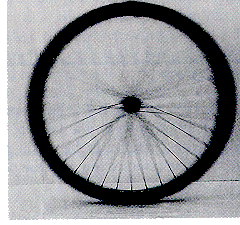
\includegraphics[scale=0.6]{figures/AngularMomentumRolling/wheel}};

}

}


\end{tikzpicture}
\captionof*{figure}{ \textit{Rolling motion. \only<2->{In rolling without slipping, the point of contact must be at rest relative to the ground.}}}
\end{center}
\end{frame}


%%%%%%%%%%%%%%%%%%%%%%%%%%%%%%%%







%%%%%%%%%%%%%%%%%%%%%%%%%%%%%%%%
\section{Rolling Without Slipping}
\label{sec:rws}
\title{Rolling Without Slipping}
\institute{Rotational Energy, Momentum and RWS}
\author{\insertsubsection}


%%%%%%%%%%%%%%%%%%%%%%%%%
\begin{frame}
\titlepage
\thispagestyle{empty}
\end{frame}

%%%%%%%%%%%%%%%%%%%%%








%%%%%%%%%%%%%%%%%%%%%%%%%%%%%%%%



%%%%%%%%%%%%%%%%%%%%%%%%%%%%%%%%


%%%%%%%%%%%%%%%%%%%%%%%%%%%%%%%%
\subsection{Modelling RWS}
\label{subsec:Modelling RWS}
\twocolframesf{Modeling rolling without slipping}
{
\only<1>{Group question}
\begin{enumerate}
\item Draw the forces on the cylinder.
\item Write the equations of motion:
\begin{itemize}
\item Sum of the forces in the $x$ direction:
\only<2>{
\begin{align*}
\sum F_x=Mg\sin\theta-f_s=Ma_{CM}
\end{align*}
}
\item Sum of the forces in the $y$ direction:
\only<2>{
\begin{align*}
\sum F_y=N-Mg\cos\theta=0
\end{align*}
}
\item Sum of the torques about the CM:
\only<2>{
\begin{align*}
\sum \tau_z=-f_sR=\frac{1}{2}MR^2\alpha
\end{align*}
}
\end{itemize}
\item<2> Can now solve for $a_{CM}, f_s, N$...
\end{enumerate}
}
{
\vspace{-1cm}
\begin{center}
\begin{tikzpicture}[scale=1]
\tikzmath{
\L=5;
\th=25;
\h=\L*tan(\th);
\d=0.8*\L/cos(\th);
\R=0.5;
}
\scalebox{1}{

\coordinate (P) at ($(\L,0)+(180-\th:\d)$);
\coordinate (PC) at ($(P)+(90-\th:\R)$);
\coordinate (OC) at ($(P)+(90-\th:2.75*\R)$);


\draw[-latex] (OC) --+(-\th:1) node[below]{$x$};
\draw[-latex] (OC) --+(90-\th:1) node[left]{$y$};

\draw[line width=1] (0,0) -- (0,\h) -- (\L,0) -- cycle;
\fill[color=myblue!40] (PC) circle(\R);
\draw ($(\L,0)-(0.7,0)$) arc(180:180-\th:0.7) node[midway,left]{\scriptsize $\theta$};

\only<2>{
\draw[-latex, line width=1.5] (PC) -- +(0,-1) node[left]{\scriptsize $\vec F_g$};
\draw[-latex, line width=1.5] (P) -- +(180-\th:0.5) node[below]{\scriptsize $\vec f_s$};
\draw[-latex, line width=1.5] (P) -- +(90-\th:0.75) node[left]{\scriptsize $\vec N$};
}


}


\end{tikzpicture}
\captionof*{figure}{ \textit{A cylinder rolling down an incline. \only<2>{If the incline is too steep, the force of static friction cannot be large enough to prevent slipping.}}}
\end{center}
\only<2>{
For rolling without slipping:
\begin{align*}
\Aboxed{a_{CM}=\alpha R}
\end{align*}

}
}


%%%%%%%%%%%%%%%%%%%%%%%%%%%%%%%%
\subsection{Instantaneous axis of rotation}
\label{subsec:instaxisofrotation}
\begin{frame}{The instantaneous axis of rotation}
\begin{itemize}
\item In rolling \textbf{without} slipping, one can choose the instantaneous axis of rotation (through the point of contact with the ground) instead of the CM to build a model.
\item About the instantaneous axis (fixed to the ground, so inertial frame of reference), the \textbf{motion is rotation only}, not the sum of rotation and translation
\item The angular velocity is the same about the CM or about the instantaneous axis!
\end{itemize}
\begin{center}
\begin{tikzpicture}[scale=1]
\tikzmath{
\R=1;
\lvcm=0.75;
}
\scalebox{1}{

\fill[color=black!50] (-\R,-\R-0.2) rectangle (11*\R,-\R);

%wheel with spokes

\foreach \x/\thth in{0/90,2.5*\R/45,5*\R/0,7.5*\R/-45,10*\R/-90}{

\draw[line width=1.5] (\x,0) circle(\R);
\fill (\x,0) circle(2pt);
\foreach \th in {0,45,...,360}{
\draw (\x,0) --+(\th:\R);
}

\draw[-latex,line width =1.5] (\x,0) -- +(\lvcm,0) node[above]{\scriptsize $\vec v_{CM}$};
\fill[color=red] ($(\x,0)+(\thth:\R)$) circle(2pt);


\ifthenelse{\thth=-90}{}{%don't draw the bottom one because it screws up the arrow of length 0
\draw [-latex, line width = 1.5,color=red] ($(\x,0)+(\thth:\R)$) -- ($ (\x,0)+(\thth:\R)+({\thth-90}:\lvcm)+(\lvcm,0)$)};

\draw [-latex, line width = 1.5, dotted]($(\x,0)+(\thth:\R)$) -- ($ (\x,0)+(\thth:\R)+({\thth-90}:\lvcm)$);
\ifthenelse{\thth=90}{\node[above right] at (0,\R) {\scriptsize $\vec v_{rot}$}}{};
}


}

\end{tikzpicture}
\captionof*{figure}{\textit{In rolling without slipping any point on the wheel can be modeled as rotating about the point of contact with the ground.}}
\end{center}
\end{frame}


%%%%%%%%%%%%%%%%%%%%%%%%%%%%%%%%
\twocolframesf{The instantaneous axis of rotation}
{
\begin{itemize}
\item About the instantaneous axis of rotation, each point is at a different distance from the axis.
\item The velocity vector for any point is perpendicular to $\vec r$ and to $\vec \omega$. It is given by:
\begin{align*}
\vec v =\vec \omega \times \vec r
\end{align*}
\item For example, the speed of the CM is given by:
\begin{align*}
v_{CM}=||\vec \omega \times \vec r_{CM}||=\omega R
\end{align*}
Which is the speed of the CM relative to the ground. \textbf{The angular velocity must be the same about the CM and about the instantaneous axis}.
\end{itemize}
}
{
\only<1>{
\begin{center}
\begin{tikzpicture}[scale=1]
\tikzmath{
\R=1;
\lvcm=0.75;
}
\useasboundingbox (-2.5*\R,-2.5*\R) rectangle (2.5*\R,2.5*\R);
\scalebox{1}{
\node at (0,2.5*\R) {\huge $\times$};
\node[above=5pt] at (0,2.5*\R) {$\vec \omega$};

\fill[color=black!50] (-2*\R,-0.2) rectangle (2*\R,0);

\draw[line width=1.5] (0,\R) circle(\R);
\fill (0,\R) circle(2pt);

\foreach \th in {45,90,...,360}{
  \draw (0,\R) -- ($(0,\R)+(\th:\R)$);
  \ifthenelse{\th=270}{
    \fill[color=red] ($(0,\R)+(\th:\R)$) circle(2pt)}{
    \draw [-latex, line width = 2,color=red] ($(0,\R)+(\th:\R)$) -- ($ (0,\R)+(\th:\R)+({\th-90}:\lvcm) +(\lvcm,0)$)
  };
 \ifthenelse{\th=360}{
   \draw [-latex, line width = 1.5](0,0) -- ($(0,\R)+(\th:\R)$) node[midway,above]{\scriptsize $\vec r$};
  }{}; 
}
}

\end{tikzpicture}
\captionof*{figure}{\textit{About the instantaneous axis of rotation, all points appear to rotate around the axis with the same angular velocity.}}
\end{center}}

\only<2>{
\begin{center}


\begin{animateinline}[autoplay,loop]{5} % 5 fps, same as 0.2 s transduration

\multiframe{24}{i=0+1}{

\begin{tikzpicture}[scale=1]

\tikzmath{
\R=1;
\lvcm=0.75;
\rotangle=\i*15;
\rcirc=sqrt(2)*\R;
}
\useasboundingbox (-2.5*\R,-2.5*\R) rectangle (2.5*\R,2.5*\R);
\scalebox{1}{

\draw[dashed] (0,0) circle(\rcirc);

\fill[color=black!50] (-2*\R,-0.2) rectangle (2*\R,0);
\fill[color=red] (0,0) circle(2pt);

\begin{scope}[rotate=-\rotangle]
\draw[line width=1.5] (0,\R) circle(\R);
\fill (0,\R) circle(2pt);

\foreach \th in {45,90,...,360}{
  \draw (0,\R) -- ($(0,\R)+(\th:\R)$); 
  \ifthenelse{\th=270}{
    \fill[color=red] ($(0,\R)+(\th:\R)$) circle(2pt)}{
    \draw [-latex, line width = 2,color=red] ($(0,\R)+(\th:\R)$) -- ($ (0,\R)+(\th:\R)+({\th-90}:\lvcm) +(\lvcm,0)$)
  };
}
\end{scope}
}
\end{tikzpicture}
%%%% end animate
}
\end{animateinline}


\captionof*{figure}{\textit{About the instantaneous axis of rotation, all points appear to rotate around the axis with the same angular velocity.}}

\end{center}
}

}


%%%%%%%%%%%%%%%%%%%%%%%%%%%%%%%%
\subsection{Modeling RWS with inst. axis}
\label{subsec:}
\twocolframesf{Modeling rolling without slipping about the instantaneous axis}
{
\begin{enumerate}
\item Draw the forces on the cylinder.
\item Write the equations of motion:
\begin{itemize}
\item Sum of the forces in the $x,y$ directions (unchanged):
\begin{align*}
\sum F_x&=Mg\sin\theta-f_s=Ma_{CM}\\
\sum F_y&=N-Mg\cos\theta=0
\end{align*}
\item Sum of the torques about the point of contact (\textbf{use parallel axis theorem} for $I$!):
\begin{align*}
\sum \tau_z=-Mg\sin\theta R=\left(\frac{1}{2}MR^2+MR^2\right)\alpha
\end{align*}
\end{itemize}
\item Can immediately determine $\alpha$ ($a_{CM}$) in this case!
\end{enumerate}
}
{
\vspace{-0.5cm}
\begin{center}
\begin{tikzpicture}[scale=1]
\tikzmath{
\L=5;
\th=25;
\h=\L*tan(\th);
\d=0.8*\L/cos(\th);
\R=0.5;
}
\scalebox{1}{

\coordinate (P) at ($(\L,0)+(180-\th:\d)$);
\coordinate (PC) at ($(P)+(90-\th:\R)$);
\coordinate (OC) at ($(P)+(90-\th:2.75*\R)$);

\draw[-latex] (OC) --+(-\th:1) node[below]{$x$};
\draw[-latex] (OC) --+(90-\th:1) node[left]{$y$};

\draw[line width=1] (0,0) -- (0,\h) -- (\L,0) -- cycle;
\fill[color=myblue!40] (PC) circle(\R);
\draw ($(\L,0)-(0.7,0)$) arc(180:180-\th:0.7) node[midway,left]{\scriptsize $\theta$};

\draw[-latex, line width=1.5] (PC) -- +(0,-1) node[left]{\scriptsize $\vec F_g$};
\draw[-latex, line width=1.5] (P) -- +(180-\th:0.5) node[below]{\scriptsize $\vec f_s$};
\draw[-latex, line width=1.5] (P) -- +(90-\th:0.75) node[left]{\scriptsize $\vec N$};
\fill[color=red] (P) circle(2pt);
}


\end{tikzpicture}
\captionof*{figure}{ \textit{A cylinder rolling down an incline, modeled using instantaneous axis of rotation.}}
\end{center}

For rolling without slipping:
\begin{align*}
\Aboxed{a_{CM}=\alpha R}
\end{align*}

}


%%%%%%%%%%%%%%%%%%%%%%%%%%%%%%%%



%%%%%%%%%%%%%%%%%%%%%%%%%%%%%%%%
\subsection{Example: giant yo-yo}
\label{subsec:giantyoyoexample}
\twocolframesf{Example: Giant Yo-Yo}
{

\only<2>{
\begin{itemize}
\item The direction of motion of the yo-yo depends on the angle with which we pull the rope
\item The direction of the force of friction is tricky to determine!
\item When the angle is low:
\begin{itemize}
\item The yo-yo goes towards the right (towards F).
\item $\vec f_s$ has to be towards the left so that the net torque about the CM is into the page. (The torque from F about the CM would make the wheel go to the left).
\end{itemize}

\end{itemize}
}
\only<3>{
\begin{itemize}
\item Sum of forces:
\begin{align*}
\sum F_x &= F\cos\theta -f_s=Ma_{CM}\\
\sum F_y &= F\sin\theta+N-Mg=0
\end{align*}
\item Sum of torques \textbf{about CM} (only $\vec F$ and $\vec f_s$):
\begin{align*}
\sum \tau_z= FR_1-f_sR_2=I\alpha
\end{align*}
\end{itemize}
\vspace{-0.5cm}
\begin{block}{Thinking about it}
\begin{itemize}
\item When the angle is small, the torque about CM from $\vec f_s$ is larger than that from $\vec F$ (yo-yo goes to the right)
\item Above some angle, the torque from $\vec f_s$ is less than that from $\vec F$ and the yo-yo goes the other way.
\item There is an angle where the net torque is zero $\rightarrow$ the yo-yo just slides
\end{itemize}
\end{block}

}

}
{
\vspace{-1cm}
\begin{center}
\begin{tikzpicture}[scale=1]
\tikzmath{
\Rb=2.25;
\Rs=1;
\th=30;
\fl=2;
}
\scalebox{1}{

\coordinate (P) at ($(0,\Rb)+(270+\th:\Rs)$);
\coordinate (OC) at (0,2.25*\Rb);

\draw[-latex] (OC) -- +(1,0) node[below]{$x$};
\draw[-latex] (OC) -- +(0,1) node[left]{$y$};

\fill[black!50] (-1.25*\Rb,-0.2) rectangle (1.25*\Rb,0);

\fill[myblue!40] (0,\Rb) circle(\Rb);
\fill[myblue!60] (0,\Rb) circle(\Rs);

\draw[-latex,line width=2] (P) -- +(\th:\fl) node[right]{$\vec F$};
\draw[dotted,line width=1] (P) -- +(2,0);
\draw ($(P) +(0.7,0)$) arc (0:\th:0.7) node[midway,right]{$\theta$};

\only<2->{
\draw[-latex,line width=2] (0,0) -- +(0,0.75) node[midway,right]{$\vec N$};
\draw[-latex,line width=2] (0,\Rb) -- +(0,-1.25) node[midway,left]{$\vec F_g$};
\draw[-latex,line width=2] (0,0) -- +(-0.75,0) node[above]{$\vec f_s$};
}

}


\end{tikzpicture}
\captionof*{figure}{ \textit{Modeling a giant yo-yo.}}
\end{center}
}

%%%%%%%%%%%%%%%%%%%%%%%%%%%%%%%%



%%%%%%%%%%%%%%%%%%%%%%%%%%%%%%%%





%%%%%%%%%%%%%%%%%%%%%%%%%%%%%%%%
\section{Angular Momentum}
\label{sec:angularmomentum}
\title{Angular Momentum}
\institute{Rotational Energy, Momentum and RWS}
\author{\insertsubsection}


%%%%%%%%%%%%%%%%%%%%%%%%%
\begin{frame}
\titlepage
\thispagestyle{empty}
\end{frame}

%%%%%%%%%%%%%%%%%%%%%





%%%%%%%%%%%%%%%%%%%%%%%%%%%%%%%%
\subsection{Formula}
\label{subsec:formulaangmomentum}
\twocolframest{Rotational dynamics – angular momemtum}
{
\begin{itemize}
\item Given an axis of rotation:
\begin{align*}
\vec r \times (\pvec F^{net} &= m\vec a)\\
\therefore \pvec \tau^{net} &=mr^2\alpha
\end{align*}
\item Rotational version of momentum (angular momentum):
\begin{align*}
\vec L&=\vec r \times \vec p\\
\frac{d\vec L}{dt}&=\frac{d}{dt} (\vec r \times \vec p) = \cancelto{0\;\;(\vec v \parallel \vec p)}{\frac{d\vec r}{dt}\times \vec p} + \vec r \times\frac{d\vec p }{dt}=\pvec \tau^{net} \\
\therefore \Aboxed{\frac{d\vec L}{dt}&=\pvec \tau^{net}} \quad\quad \text{compare to}\quad\quad \frac{d\vec p}{dt}=\pvec F^{net}
\end{align*}
\end{itemize}

}
{
\begin{center}
\begin{tikzpicture}[scale=1]
\tikzmath{}
\scalebox{1}{

\fill (0,0) circle (2pt) node[below]{axis};

\draw[-latex,line width = 2] (0,0) -- (30:2) node[midway, below]{$\vec r$};
\fill (30:2) circle (4pt) node[right=5pt]{$m$};
\draw[-latex,line width = 2] (30:2) -- +(120:1.5) node[midway, right]{$\vec p$};

}

\end{tikzpicture}
\captionof*{figure}{\textit{Angular momentum is defined for a particular axis of rotation based on the particle's momentum.}}
\end{center}
}


%%%%%%%%%%%%%%%%%%%%%%%%%%%%%%%%
\subsection{Expressing angular momentum}
\label{subsec:}
\twocolframest{Angular momentum of particle}
{
\begin{itemize}
\item If there is \textbf{no net torque} about an axis on the mass, then its \textbf{angular momentum relative to that axis is conserved}.
\item There could be a net force on the particle (momentum is not conserved), but if the net force is in such a way that it produces no net torque (\textbf{about a given point}), then angular momentum (\textbf{about that given point}) is conserved.
\item Angular momentum measures how much ``rotation'' a particle has about a particular axis. 
\item[$\rightarrow$] If the particle has no angular velocity about that axis, it has no angular momentum about that axis.
\item[$\rightarrow$] If the particle is further from axis or more massive, it has more angular momentum.
\end{itemize}
}
{
\begin{center}
\begin{tikzpicture}[scale=1]
\tikzmath{}
\scalebox{1}{

\fill (0,0) circle (2pt) node[below]{axis};
\fill (90:3) circle (4pt) node[right=5pt]{$m$};


\draw[latex-,line width = 2] (90:3) -- +(0,-1)  node[midway, right]{$\vec F$};



}

\end{tikzpicture}
\captionof*{figure}{\textit{In this case, linear momentum is not conserved while angular momentum about the given axis is conserved.}}
\end{center}
}


%%%%%%%%%%%%%%%%%%%%%%%%%%%%%%%%
\twocolframest{Angular momentum of a system}
{
\begin{itemize}
\item We summed the momenta of the particles in a system:
\begin{align*}
\frac{d\vec p_i}{dt}&=\pvec F^{net}\\
\therefore \frac{d\vec P}{dt}&=\pvec F^{ext}
\end{align*}
\item We do the same for angular momentum:
\begin{align*}
\frac{d\vec L_i}{dt}&=\pvec \tau^{net}\\
\therefore \frac{d\vec L}{dt}&=\pvec \tau^{ext}
\end{align*}
\item If there is \textbf{no net external torque on a system}, the angular momentum of the system is conserved
\end{itemize}
}
{
\begin{center}
\begin{tikzpicture}[scale=1]
\tikzmath{}
\scalebox{1}{

\fill (0,0) circle (2pt) node[below]{axis};
\fill (90:3) circle (3pt);
\draw[-latex,line width = 1] (90:3) -- +(70:2);

\fill (45:1) circle (3pt);
\draw[-latex,line width = 1] (45:1) -- +(140:1.5);

\fill (75:2) circle (3pt);
\draw[-latex,line width = 1] (75:2) -- +(-45:1);
}

\end{tikzpicture}
\captionof*{figure}{\textit{The total angular momentum is the sum of the angular momenta of the particles in the system.}}
\end{center}
}


%%%%%%%%%%%%%%%%%%%%%%%%%%%%%%%%
\begin{frame}{Angular momentum for a solid object}
\begin{itemize}
\item For a single particle in a system its angular momentum about an axis of rotation is:
\begin{align*}
\vec L_i = \vec r_i\times \vec p_i = \vec r_i \times m_i\vec v_i=m_i \vec r_i \times (\vec \omega \times\vec r_i)=m_ir_i^2\vec \omega
\end{align*}
\item Adding together the angular momenta of particles in a solid object (all with the same angular velocity):
\begin{align*}
\vec L &= \left(\sum_i m_ir_i^2 \right) \vec \omega\\
\Aboxed{\vec L &=I\vec\omega}
\end{align*}
\end{itemize}

\end{frame}


%%%%%%%%%%%%%%%%%%%%%%%%%%%%%%%%
\subsection{Angular in relation to linear quantities}
\label{subsec:correspondencetable}
\begin{frame}{Correspondence between linear and angular}
\begin{tabular}{llll}
\textbf{Name} &\textbf{Linear} & \textbf{Angular} & \textbf{Correspondence}\\
\hline\hline
Displacement & $s$ & $\vec \theta$ & $d\vec\theta=\frac{1}{r^2} \vec r\times d\vec s$  \\
Velocity & $\vec v$ & $\vec \omega$ & $\vec\omega=\frac{1}{r^2} \vec r\times \vec v$, $v_T = \vec\omega\times \vec r$ \footnote{This corresponds to the component of velocity perpendicular to $\vec r$.}\\
Acceleration & $\vec a$ & $\vec \alpha$ & $\vec\alpha=\frac{1}{r^2} \vec r\times \vec a$, $a_T = \vec\alpha\times \vec r$ \footnote{This corresponds to the component of acceleration perpendicular to $\vec r$.}\\
Inertia& $m$ & $I$ & $I=\sum_i m_ir_i^2$ \\
Momentum& $\vec p=m\vec v$& $\vec L = I\vec \omega$ &$\vec L = \vec r\times \vec p$ \\
Newton's Second Law&$\pvec F^{ext}=m\vec a_{CM}$ & $\pvec \tau^{ext} = I\vec\alpha$& $\vec F \to \vec\tau$, $m\to I$, $\vec a \to \vec \alpha$\\
Newton's Second Law& $\frac{d\vec p}{dt} =\pvec F^{ext}$ & $\frac{d\vec L}{dt} =\pvec \tau^{ext}$&$\vec F \to \vec\tau$, $\vec p \to \vec L$ \\
Kinetic energy&$\frac{1}{2}mv^2$ &$\frac{1}{2}I\omega^2$ &$m\to I$, $v\to \omega$ \\
Power&$\vec F \cdot \vec v$ &$\vec \tau \cdot \vec\omega$ &$\vec F \to \vec\tau$, $\vec v\to \vec\omega$  \\
\end{tabular}
\end{frame}


%%%%%%%%%%%%%%%%%%%%%%%%%%%%%%%%


%%%%%%%%%%%%%%%%%%%%%%%%%%%%%%%%
\subsection{Planets and the solar system}
\label{subsec:planets and the solar system}
\twocolframesf{Planets and the solar system}
{
\begin{itemize}
\item The solar system started off as a very big roughly spherical ball of gas with atoms moving in all directions.
\item Since the motion of the atoms was random, there was a net total angular momentum in some direction.
\item Atoms and matter coalesced because of gravity towards the centre of mass:
\begin{itemize}
\item Their rotational speed had to increase (moment of inertia got smaller).
\item They all ended up in the same plane (perpendicular to angular momentum of the system), mostly due to collisions.
\end{itemize}
\end{itemize}
}{
\capfig{1}{figures/AngularMomentumRolling/solarsystem}{Through conservation of angular momentum, all planet orbit in a similar plane. \scriptsize \url{https://jcconwell.wordpress.com/tag/angular-momentum/}}
}

%%%%%%%%%%%%%%%%%%%%%%%%%%%%%%


%%%%%%%%%%%%%%%%%%%%%%%%%%%%%%%%

%%%%%%%%%%%%%%%%%%%%%%%%%%%%%%%%
\subsection{Example: bicycle wheel}
\label{subsec:bicyclewheelexample}
\twocolframe{Example: Bicycle wheel}
{Tilt the axis of the wheel!}
{

\begin{center}
\begin{tikzpicture}[scale=1]
\tikzmath{
\R=1.5;
}
\scalebox{1}{

\draw[-latex, line width=1] ($(-0.5*\R,0)+(80:{0.75*\R/4} and {0.75*\R})$) arc (80:240:{0.75*\R/4} and {0.75*\R});
\draw[line width=1,dashed] (-\R,0) -- (\R,0);
\draw[line width=1] (0,0) circle(\R/4 and \R);
\draw[line width=2] (0,\R) arc (90:270:\R/4 and \R);
\foreach \th in {0,30,...,330}{
\draw (0,0) -- (\th:\R/4 and \R);
}
\draw[-latex,line width=2] (0.5*\R,0) -- +(\R,0) node[midway,above]{$\vec L$};

}

\end{tikzpicture}

\end{center}
}



%%%%%%%%%%%%%%%%%%%%%%%%%%%%%%%%
\twocolframefs{Tilting the bicycle wheel requires exerting a torque}
{
\begin{itemize}
\item If you try to change the axis of rotation, you have to exert a torque to change the angular momentum.
\begin{align*}
\vec \tau = \frac{d\vec L}{dt}\sim\frac{\Delta\vec L}{\Delta  t}
\end{align*}
\item If you let the wheel hang, gravity tries to rotate the axis of rotation $\rightarrow$ precession.
\end{itemize}
}
{
\begin{center}
\begin{tikzpicture}[scale=1]
\tikzmath{
\R=1.5;
\throt=20;
}
\scalebox{1}{

\draw[-latex, line width=1] ($(-0.5*\R,0)+(80:{0.75*\R/4} and {0.75*\R})$) arc (80:240:{0.75*\R/4} and {0.75*\R});
\draw[line width=1,dashed] (-\R,0) -- (\R,0);
\draw[line width=1] (0,0) circle(\R/4 and \R);
\draw[line width=2] (0,\R) arc (90:270:\R/4 and \R);
\foreach \th in {0,30,...,330}{
\draw (0,0) -- (\th:\R/4 and \R);
}
\draw[-latex,line width=2] (0.5*\R,0) -- +(\R,0) node[midway,above]{$\vec L$};


\begin{scope}[shift={(3*\R,0)},rotate=\throt]
\draw[line width=1,dashed] (-\R,0) -- (\R,0);
\draw[line width=1] (0,0) circle(\R/4 and \R);
\draw[line width=2] (0,\R) arc (90:270:\R/4 and \R);
\foreach \th in {0,30,...,330}{
\draw (0,0) -- (\th:\R/4 and \R);
}
\draw[-latex,line width=2] (0.5*\R,0) -- +(\R,0) node[midway,above]{$\pvec L'$};
\draw[-latex, line width=1] ($(0.5*\R,0)+(80:{0.75*\R/4} and {0.75*\R})$) arc (80:240:{0.75*\R/4} and {0.75*\R});
\end{scope}

\begin{scope}[shift={(0,-2*\R)}]

\draw[-latex,line width=2] (0,0) -- +(1.5*\R,0) node[midway,below]{$\vec L$};
\draw[-latex,line width=2] (0,0) -- +(\throt:1.5*\R) node[midway,above]{$\pvec L'$};
\draw[-latex,line width=2] (1.5*\R,0) -- (\throt:1.5*\R) node[midway,right]{$\Delta \vec L $};

\draw[-latex,line width=2] (2.5*\R,-0.25*\R) -- +({90+\throt/2}:\R) node[midway,right]{$\vec \tau$};
\begin{scope}[shift={(2.5*\R,-0.25*\R)},rotate={\throt/2}]
\draw[-latex, line width=1] ($(0,0)+(180:{0.5*\R} and {0.5*\R/4})$) arc (180:430: {0.5*\R} and {0.5*\R/4});
\end{scope}

\end{scope}

}

\end{tikzpicture}
\captionof*{figure}{\textit{Tilting the horizontal axis of a spinning wheel requires a torque in the vertical direction!}}
\end{center}
}

%%%%%%%%%%%%%%%%%%%%%%%%%%%%%%%%



















































%%%%%%%%%%%%%%%%%%%%%%%%%%%%%%%%

\title{Simple Harmonic Motion}
\subject{Form, Examples and Modelling}
\subtitle{Building Models to Describe our World}



%%%%%%%%%%%%%%%%%%%%%%%%%
%%%%%% Title slide %%%%%%
%%%%%%%%%%%%%%%%%%%%%%%%%
\chaptertitle{Simple Harmonic Motion}
\begin{frame}
\label{chap:simpleharmonicmotion}
\titlepage
\thispagestyle{empty}

\begin{textblock*}{5cm}(11cm,4cm)
    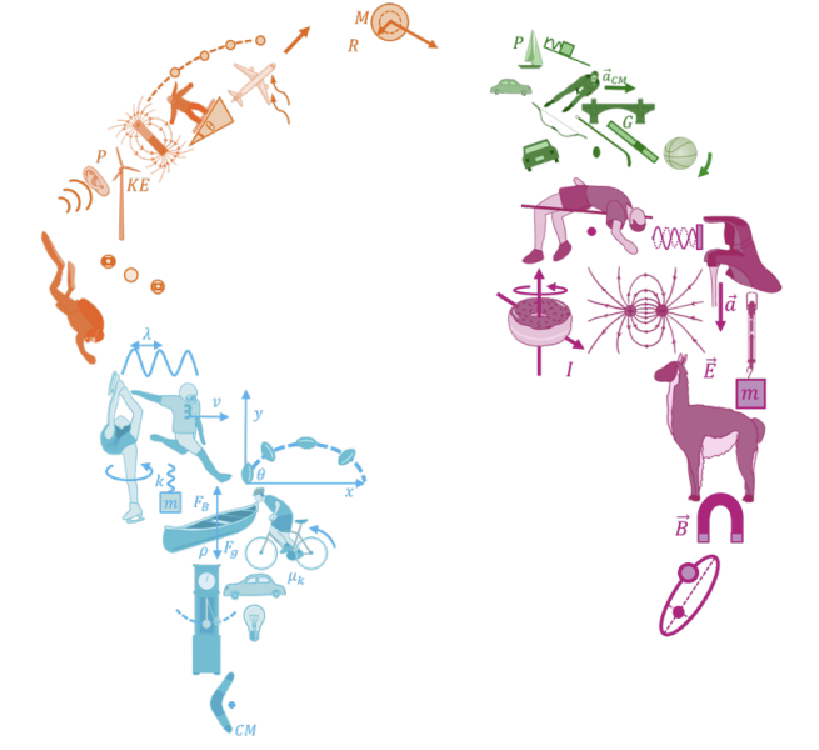
\includegraphics[width=4cm]{figures/BMDW/logo}
\end{textblock*}

\end{frame}

%%%%%%%%%%%%%TOC

\twocolframe{Outline}
{\tableofcontents[sections=34-35, subsectionstyle=show/show]\thispagestyle{empty}}
{\tableofcontents[sections=36, subsectionstyle=show/show]}

%%%%%%%%%%%%%%%%%%%%%%%%%











%%%%%%%%%%%%%%%%%%%%%%%%%%%%%%%%
\section{The Structure of SHM}
\label{sec:shhstructure}
\title{The Structure of SHM}
\institute{Simple Harmonic Motion}
\author{\insertsubsection}


%%%%%%%%%%%%%%%%%%%%%%%%%
\begin{frame}
\titlepage
\thispagestyle{empty}
\end{frame}

%%%%%%%%%%%%%%%%%%%%%%%%









%%%%%%%%%%%%%%%%%%%%%%%%%%%
\subsection{The concept and formula}
\label{subsec:conceptandformulashm}
\begin{frame}{Simple Harmonic Motion}
\begin{itemize}
\item Anytime that you have this equation of motion:
\begin{align*}
\frac{d^2x}{dt^2}=-\omega^2 x
\end{align*}
\item We call the motion ``Simple Harmonic Motion'' and the solution is:
\begin{align*}
x(t)=A\cos(\omega t +\phi)
\end{align*}
(note that sine also works)
\item Where $A$ and $\phi$ are ``integration constants'' that depend on the specific ``initial conditions''.
\end{itemize}

\end{frame}

%%%%%%%%%%%%%%%%%%%%%%%%%%%%%%%%


%%%%%%%%%%%%%%%%%%%%%%%%%%%%%%%%
\subsection{Application example: spring-mass system}
\label{subsec:springmassexample}
\twocolframesf{Applications of SHM: spring-mass system}
{
\only<1>{
\begin{itemize}
\item The equation of motion for SHM comes up \textit{a lot} in physics.
\item The most obvious case is to describe the position of a mass attached to a spring:
\begin{align*}
ma&=-kx\\
m\frac{d^2x}{dt^2}&=-k x\\
\therefore \frac{d^2x}{dt^2}&=-\frac{k}{m}x=-\omega^2 x\\
\omega&=\sqrt{\frac{k}{m}}
\end{align*}
\end{itemize}
}
\only<2>{
\begin{itemize}
\item The position as a function of time is given by:
\begin{align*}
x(t)=A\cos(\omega t +\phi)
\end{align*}
\item The velocity as a function of time is given by:
\begin{align*}
v(t)=\frac{dx}{dt}=-A\omega\sin(\omega t +\phi)
\end{align*}
\item Need to determine $A$ and $\phi$ from initial conditions:
\begin{itemize}
\item[$\rightarrow$] Specify (say) position and velocity at $t=0$.
\end{itemize}

\end{itemize}

}
}
{

\begin{center}
\begin{tikzpicture}[scale=1]
\tikzmath{
\L=2.;
\dx=0.75*\L;
\off=0.5;
\h=1;
}
\scalebox{1}{


\draw[line width=1.5pt] (-1.5*\L,0) -- (1.5*\L,0) ;
\draw[line width=1.5pt] (0,-0.1) -- (0,0.1);
\node[below] at (0,0) {$0$};

\fill (-1.5*\L,0) rectangle (-1.4*\L,\h);
\draw[decoration={aspect=0.3, segment length=2.8mm, amplitude=3mm,coil},decorate,line width=1pt] (-1.4*\L,\h/2) -- (0,\h/2);
%\draw [latex-latex] (-1.4*\L,\h) -- (0,\h) node[midway,above]{$L_0$};
\fill[myblue!60] (0,0) rectangle (\h,\h);

%%%%%%%%%%  top compressed
\begin{scope}[shift={(0,1.5*\h)}]
\draw[line width=1.5pt] (-1.5*\L,0) -- (1.5*\L,0);
\draw[line width=1.5pt] (0,-0.1) -- (0,0.1);
\node[below] at (0,0) {$0$};
\draw[line width=1.5pt] (-\dx,0.1) -- +(0,-0.2)node[below]{$-A$};

\fill (-1.5*\L,0) rectangle (-1.4*\L,\h);
\draw[decoration={aspect=0.3, segment length=2mm, amplitude=3mm,coil},decorate,line width=1pt] (-1.4*\L,\h/2) -- (-\dx,\h/2);
%\draw [color=blue,latex-latex] (-\dx,1.2*\h) -- (0,1.2*\h) node[midway,above]{$x<0$};
\fill[myblue!60] (-\dx,0) rectangle (-\dx+\h,\h);
%\draw[line width=2, -latex, color=myred] (-\dx,\h/2) -- +(1.3,0) node[right] {$\vec F$};

\end{scope}
%%%%%%%%%% bottom extended
\begin{scope}[shift={(0,-1.5*\h)}]
\draw[-latex,line width=1.5pt] (-1.5*\L,0) -- (1.5*\L,0) node[below]{$x$};
\draw[line width=1.5pt] (0,-0.1) -- (0,0.1);
\node[below] at (0,0) {$0$};
\draw[line width=1.5pt] (\dx,0.1) -- +(0,-0.2)node[below]{$A$};

\fill (-1.5*\L,0) rectangle (-1.4*\L,\h);
\draw[decoration={aspect=0.3, segment length=3.5mm, amplitude=3mm,coil},decorate,line width=1pt] (-1.4*\L,\h/2) -- (\dx,\h/2);
%\draw [color=blue,latex-latex] (0,\h) -- (\dx,\h) node[midway,above]{$x>0$};
\fill[myblue!60] (\dx,0) rectangle (\dx+\h,\h);
%\draw[line width=2, -latex, color=myred] (\dx,\h/2) -- +(-1.3,0) node[midway,below=-2pt] {$\vec F$};
\end{scope}

}
\end{tikzpicture}
\captionof*{figure}{\textit{A spring-mass system is a common example of simple harmonic motion.}}
\end{center}


}


%%%%%%%%%%%%%%%%%%%%%%%%%%%%%%%%
\subsection{Integration constants}
\label{subsec:integrationconstants}
\begin{frame}{Specifying the integration constants}
\begin{align*}
\frac{d^2x}{dt^2}=-\omega^2 x
\end{align*}
\begin{itemize}
\item This is a second order differential equation, so we must specify 2 integration constants.
\item At some time, $t=t_0$, we specify the initial position, $x_0$, and initial velocity, $v_0$.
\item This is enough information to determine $A$ and $\phi$  (say $t_0=0$):
\begin{align*}
x_0&=x(0)=A\cos(\omega t_0 +\phi)=A\cos(\phi)\\
v_0&=v(0)=-A\omega\sin(\omega t_0 +\phi)=-A\omega\sin(\phi)
\end{align*}
\item Similar to:
\begin{align*}
\frac{d^2x}{dt^2}=a \quad\quad x(t)=x_0+v_0t+\frac{1}{2}at^2
\end{align*}
where we specify initial position, $x_0$, and initial velocity, $v_0$
\end{itemize}

\end{frame}


%%%%%%%%%%%%%%%%%%%%%%%%%%%%%%%%


%%%%%%%%%%%%%%%%%%%%%%%%%%%%%%%%



%%%%%%%%%%%%%%%%%%%%%%%%%%%%%%%%
\subsection{SHM in in relation to rotational motion}
\label{subsec:shmplusrm}
\twocolframesf{Back to rotational motion}
{
\begin{itemize}
\item The position of the simple harmonic oscillator is described by the \textbf{same function} as the $x$ or $y$ position of a particle moving around a circle of radius $A$ at constant angular velocity.
\item The phase, $\phi$, tells you where on the circle it started at time $t=0$ (it's like $\theta_0$).
\item Depending on the context, we call, $\omega$, the \textbf{angular frequency} or the \textbf{angular velocity} – we use the terms interchangeably.
\end{itemize}
\begin{align*}
x(t)&=A\cos(\omega t+\phi)=A\cos\left(\theta(t)\right)\\
\theta(t)&=\phi+\omega t
\end{align*}
}
{
\vspace{-1cm}
\begin{center}

\begin{animateinline}[autoplay,loop]{5} % 5 fps, same as 0.2 s transduration

\multiframe{24}{i=1+1}{

\begin{tikzpicture}[scale=1]
\tikzmath{
\R=1.5;
\h=2*\R;
\th=\i*15;
\x=\R*cos(\th);
}

\useasboundingbox (-2*\R,-2.5*\R) rectangle (2*\R,1.5*\R);
\scalebox{1}{
\draw[-latex] (0,0) -- (1.25*\R,0) node[below]{$x$};
\draw[-latex] (0,0) -- (0,1.25*\R) node[left]{$y$};
\draw[line width=1] (0,0) circle (\R);

\fill (\th:\R) circle(2pt);


\draw[-latex,line width=1] (-1.5*\R,-\h) -- (1.5*\R,-\h) node[below]{$x$};

\draw[line width=1] (-\R,-\h+0.1) -- +(0,-0.2) node[below]{$-A$};
\draw[line width=1] (0,-\h+0.1) -- +(0,-0.2) node[below]{$0$};
\draw[line width=1] (\R,-\h+0.1) -- +(0,-0.2) node[below]{$A$};

\fill (\x,-\h) circle(2pt);

\draw[dashed] (\x,-\h) -- (\th:\R);
\draw[-latex, line width=2] (0,0) -- (\th:\R);
\draw[color=red,-latex] (0.7,0) arc(0:\th:0.7);

}
\end{tikzpicture}
}
\end{animateinline}


\captionof*{figure}{\textit{The linear displacement of a spring in SHM is the same as $x$ position of an object in uniform circular motion.}}
\end{center}
}

%%%%%%%%%%%%%%%%%%%%%%%%%%%%%%%%
\begin{frame}{Simple Harmonic Motion}
\begin{itemize}
\item Any physics model that gives:
\begin{align*}
\frac{d^2x}{dt^2}=-\omega^2 x
\end{align*}
is said to correspond to simple harmonic motion and is described by the same math. 
\item SHM arises from physics where there is a \textbf{restoring force} that is \textbf{linearly proportional to displacement}. For example, $F=-kx$.
\item All of the physics is contained in $\omega$, the angular frequency of the motion. 
\item For a mass on a spring:
\begin{align*}
\omega=\sqrt{\frac{k}{m}}
\end{align*}
$\rightarrow$ The frequency of the oscillations depends on how stiff the spring is and how heavy the mass is – nothing else!

\end{itemize}

\end{frame}


%%%%%%%%%%%%%%%%%%%%%%%%%%%%%%%%







%%%%%%%%%%%%%%%%%%%%%%%%%%%%%%%%
\section{Spring Systems}
\label{sec:springs}
\title{Spring Systems}
\institute{Simple Harmonic Motion}
\author{\insertsubsection}


%%%%%%%%%%%%%%%%%%%%%%%%%
\begin{frame}
\titlepage
\thispagestyle{empty}
\end{frame}

%%%%%%%%%%%%%%%%%%%%%%%%





\subsection{Vertical spring system}
\label{subsec:verticalspringsystem}
\twocolframesf{Vertical mass on a spring}
{
\vspace{-0.25cm}
\only<1>{
}

\only<2>{
\begin{itemize}
\item Observations:
\begin{itemize}
\item The mass oscillates about the equilibrium position, not the rest position of the spring.
\item It feels like SHM, so maybe it is?
\end{itemize}
\item The math doesn't quite look like SHM:
\begin{align*}
mg-ky&=ma_y\\
\frac{d^2y}{dt^2}&=g-\frac{k}{m}y
\end{align*}
not the same as:
\begin{align*}
\frac{d^2y}{dt^2}=-\frac{k}{m}y
\end{align*}
\end{itemize}
}

\only<3>{
\begin{itemize}
\item Consider changing coordinate system, so that the origin is located at the point about which the mass oscillates:
\begin{align*}
y'=y-y_0
\end{align*}
\item The extension of the spring is thus:
\begin{align*}
y=y'+y_0
\end{align*}
\item In terms of $y'$, Newton's Second Law reads:
\begin{align*}
\frac{d^2y}{dt^2}&=g-\frac{k}{m}y\\
\frac{d^2(y'+y_0)}{dt^2}&=g-\frac{k}{m}(y'+y_0)
\end{align*}
\end{itemize}
}

\only<4>{
\begin{itemize}
\item Starting from:
\begin{align*}
\frac{d^2(y'+y_0)}{dt^2}&=g-\frac{k}{m}(y'+y_0)\\
\frac{d^2y'}{dt^2}&=g-\frac{k}{m}y'-\frac{k}{m}y_0
\end{align*}
\item At the equilibrium point, the spring is extended by $y_0$, and the spring force is equal to gravity:
\begin{align*}
mg-ky_0 = 0 \quad \rightarrow \quad \frac{k}{m}y_0=g
\end{align*}
and we recover SHM using the $y'$ axis:
\begin{align*}
\frac{d^2y'}{dt^2}&=\frac{k}{m}y'
\end{align*}
\end{itemize}
}

}
{
\vspace{-0.25cm}
\begin{center}
\begin{tikzpicture}[scale=1]
\tikzmath{
\L=2.;
\dx=0.6*\L;
\abox=0.75;
}
\scalebox{1}{

\only<3->{
\draw[-latex,line width=1.5,color=red] (-4*\abox,0.5*\abox) -- +(0,-2.5*\L) node[left]{$y'$};
\draw[line width=1,color=red] (-4*\abox-0.1,-\L) node[left]{0} -- +(0.2,0) ;
\draw[line width=1,color=red] (-4*\abox-0.1,-\L-\dx) node[left]{$y'$} -- +(0.2,0) ;
}

\draw[-latex,line width=1.5] (-3*\abox,0.5*\abox) -- +(0,-2.5*\L) node[left]{$y$};
\draw[dashed] (-1.5*\abox,-\dx) -- (-3*\abox,-\dx);
\draw[line width=1] (-3*\abox-0.1,-\dx) node[left]{0} -- +(0.2,0) ;

\draw[dashed] (0,-\L) -- (-3*\abox,-\L);
\draw[line width=1] (-3*\abox-0.1,-\L) node[left]{$y_0$} -- +(0.2,0) ;

\draw[dashed] (1.5*\abox,-\L-\dx) -- (-3*\abox,-\L-\dx);
\draw[line width=1] (-3*\abox-0.1,-\dx-\L) node[left]{$y$} -- +(0.2,0) ;

%middle
\fill (-0.5*\abox,0) rectangle (0.5*\abox,0.2);
\draw[decoration={aspect=0.3, segment length=3mm, amplitude=3mm,coil},decorate,line width=1pt] (0,0) -- +(0,-\L);
\fill[myblue!60] (-\abox/2,-\L) rectangle +(\abox,-\abox);
%FBD
\coordinate (P) at (\abox,-\L-\abox/2);
\fill (P) circle(3pt);
\draw[-latex,line width=1.5] (P) -- +(0,1) node[above]{\scriptsize $\vec F(y_0)$};
\draw[-latex,line width=1.5] (P) -- +(0,-1) node[left]{\scriptsize $\vec F_g$};


%%%%%%%%%%%  top compressed
\begin{scope}[shift={(-1.5*\abox,0)}]
\fill (-0.5*\abox,0) rectangle (0.5*\abox,0.2);
\draw[decoration={aspect=0.3, segment length=1.7mm, amplitude=3mm,coil},decorate,line width=1pt] (0,0) -- +(0,-\dx);
%\fill[myblue!60] (-\abox/2,-\dx) rectangle +(\abox,-\abox);

\end{scope}

%%%%%%%%%%% bottom extended
\begin{scope}[shift={(2.*\abox,0)}]
\fill (-0.5*\abox,0) rectangle (0.5*\abox,0.2);
\draw[decoration={aspect=0.3, segment length=5mm, amplitude=3mm,coil},decorate,line width=1pt] (0,0) -- +(0,-\dx-\L);
\fill[myblue!60] (-\abox/2,-\dx-\L) rectangle +(\abox,-\abox);
%FBD:
\coordinate (P2) at (\abox,-\L-\dx-\abox/2);
\fill (P2) circle(3pt);
\draw[-latex,line width=1.5] (P2) -- +(0,1.5) node[above]{\scriptsize $\vec F(y)$};
\draw[-latex,line width=1.5] (P2) -- +(0,-1) node[left]{\scriptsize $\vec F_g$};
\end{scope}

}
\end{tikzpicture}
\captionof*{figure}{\textit{A vertical spring-mass system. In the middle position, the force of gravity has the same magnitude as the spring force and the system is in equilibrium.}}
\end{center}

}









%%%%%%%%%%%%%%%%%%%%%%%%%%%%%%%%
\subsection{Constant force + spring force}
\label{subsec:cnsthforceplusspringforce}
\twocolframesf{Constant force + spring force = SHM}
{
\begin{itemize}
\item For a vertical spring-mass, we had an equation of the form:
\begin{align*}
F-kx=m\frac{d^2x}{dt^2}
\end{align*}
where $F$ is a constant force (like gravity).
\item We saw that if we define a new equilibrium position (not the rest position of the spring), then we can recover simple harmonic motion about that point. 
\item With two springs attached to a mass, it's the same idea, and one also recovers SHM $\rightarrow$ in this case the ``effective'' spring constant is $k=k_1+k_2$.
\end{itemize}
}
{
\begin{center}
\begin{tikzpicture}[scale=1]
\tikzmath{
\L=1.75;
\dx=0.75*\L;
\off=0.5;
\h=1;
\x1=-0.6*\L;
\x2=0.8*\L;
}
\scalebox{1}{


\draw[line width=1.5pt] (-1.5*\L,0) -- (1.5*\L,0) ;

\draw[line width=1.5pt,-latex] (-1.6*\L,-0.5) -- (1.6*\L,-0.5) node[below]{$x$};
\draw[line width=1.5pt] (-1.5*\L,-0.4) -- +(0,-0.2) node[below] {$0$};

\draw[dashed] (\x1,\h/2) -- (\x1,-0.5);
\draw[line width=1.5pt] (\x1,-0.4) -- +(0,-0.2) node[below] {$x_1$};

\draw[dashed] (\x2,\h/2) -- (\x2,-0.5);
\draw[line width=1.5pt] (\x2,-0.4) -- +(0,-0.2) node[below] {$x_2$};

\fill (-1.5*\L,0) rectangle (-1.4*\L,\h);
\fill (1.4*\L,0) rectangle (1.5*\L,\h);

\draw[decoration={aspect=0.3, segment length=1.8mm, amplitude=3mm,coil},decorate,line width=1pt] (-1.4*\L,\h/2) -- (\x1,\h/2) node[midway, above=10pt]{$k_1$};
\draw[decoration={aspect=0.3, segment length=1.8mm, amplitude=3mm,coil},decorate,line width=1pt] (\x2,\h/2) -- (1.4*\L,\h/2) node[midway, above=10pt]{$k_2$};

\draw[dashed] (-0.1*\L+\h/2,-0.5)node[above]{$x_0$} -- +(0,-2*\h+0.5) ;
\draw[latex-latex] (\x1,-1.25*\h) -- (-0.1*\L+\h/2,-1.25*\h) node[midway,below]{\scriptsize $x_0-x_1$};
\draw[latex-latex] (\x2,-1.25*\h) -- (-0.1*\L+\h/2,-1.25*\h) node[midway,below]{\scriptsize $x_2-x_0$};

\begin{scope}[shift={(0,-3.*\h)}]

\draw[line width=1.5pt] (-1.5*\L,0) -- (1.5*\L,0) ;
\fill (-1.5*\L,0) rectangle (-1.4*\L,\h);
\fill (1.4*\L,0) rectangle (1.5*\L,\h);

\draw[decoration={aspect=0.3, segment length=2.8mm, amplitude=3mm,coil},decorate,line width=1pt] (-1.4*\L,\h/2) -- (-0.1*\L,\h/2);
\draw[decoration={aspect=0.3, segment length=2.8mm, amplitude=3mm,coil},decorate,line width=1pt] (-0.1*\L+\h,\h/2) -- (1.4*\L,\h/2) ;

\fill[myblue!60] (-0.1*\L,0) rectangle +(\h,\h);

\end{scope}

}
\end{tikzpicture}
\captionof*{figure}{\textit{A mass connected to two springs}}
\end{center}
At equilibrium:
\begin{align*}
k_1(x_0-x_1)+k_2(x_2-x_0)=0
\end{align*}

}


%%%%%%%%%%%%%%%%%%%%%%%%%%%%%%%%
%%%%%%%%%%%%%%%%%%%%%%%%%%%%%%%%

\section{Pendulums and Approxomations}
\label{sec:pendulums}
\title{Pendulums and Approxomations}
\institute{Simple Harmonic Motion}
\author{\insertsubsection}


%%%%%%%%%%%%%%%%%%%%%%%%%
\begin{frame}
\titlepage
\thispagestyle{empty}
\end{frame}

%%%%%%%%%%%%%%%%%%%%%%%%
\subsection{Motion of pendulums}
\label{subsec:motionofpendulums}
\twocolframesf{Motion of a pendulum is also SHM}
{
\begin{itemize}
\item The torque from gravity (about the origin) is a \textit{restoring torque} (it tries to bring the pendulum back to equilibrium):
\begin{align*}
\vec \tau_g=-mg\sin\theta L\hat z
\end{align*}
\item Rotational version of Newton's Second Law:
\begin{align*}
\sum \vec \tau=\vec \tau_g&=-mL^2\vec\alpha\\
-mg\sin\theta L &=mL^2\frac{d^2\theta}{dt^2}\\
\frac{d^2\theta}{dt^2}&=-\frac{g}{L}\sin\theta
\end{align*}
not quite SHM...
\end{itemize}
}
{
\vspace{-1cm}
\begin{center}
\begin{tikzpicture}[scale=1]
\tikzmath{
\L=2;
\th=30;
}
\scalebox{1}{
\coordinate (P) at (270+\th:\L);
\draw[-latex] (0.0*\L,0) -- +(0.5,0) node[below]{$x$};
\draw[-latex] (0.*\L,0) -- +(0,0.5) node[left]{$y$};
\fill (0,0) circle (2pt);
\fill (P) circle (4pt) node[right=5pt]{$m$};
\draw[line width=1] (0,0) -- (P) ;
\draw[dotted,line width=1] (0,0) -- +(0,-\L) node[midway, left]{$L$};
\draw[dashed] (\L,0) arc (0:-180:\L);

\draw[-latex, line width=2] (P) -- +(90+\th:1.2) node[right=5pt]{$\vec T$};
\draw[-latex, line width=2] (P) -- +(0,-1) node[right]{$\vec F_g$};

\draw (0,-0.7) arc (270:270+\th:0.7) node[midway,below]{$\theta$};

}
\end{tikzpicture}
\captionof*{figure}{\textit{Modeling a pendulum, using torque from gravity.}}
\end{center}
\only<2>{
\vspace{-0.5cm}
\begin{block}{Small angle approximation}
To get SHM, need to approximate $\sin\theta\sim\theta$, then:
\begin{align*}
\frac{d^2\theta}{dt^2}&\sim -\frac{g}{L}\theta \quad\rightarrow\quad \omega=\sqrt{\frac{g}{L}}\\
\therefore \theta(t) &= A\cos(\omega t+\phi)
\end{align*}
\end{block}
}
}


%%%%%%%%%%%%%%%%%%%%%%%%%%%%%%%%
\subsection{Small angle approxomations}
\label{subsec:smallangles}
\begin{frame}{What does it mean for $\theta$ to be small?}
\begin{itemize}
\item How small is small?
\item You try it out on your calculator...  has to be in radians for this to work...
\item If the angle is too big, then it's not SHM anymore. We'll do a lab next semester to figure this out. It turns out that SHM is a very good approximation even to relatively large angles.
\end{itemize}
\begin{columns}

\column{0.5\textwidth}
\begin{center}
\begin{tikzpicture}[scale=1]
\tikzmath{
\L=5;
\th=20;
\h=\L*sin(\th);
}
\scalebox{1}{
\draw[line width=1.5] (0,0) -- (\L,0) node[midway,below] {$R=1$} arc(0:\th:\L) node[midway,left]{$s$}-- cycle;
\draw[line width=1.5,color=red,dotted] (\L,0) -- +(0,\h) node[midway,right]{$x$} -- (0,0);

\draw (1,0) arc(0:\th:1) node[midway,right]{$\theta$};
}
\end{tikzpicture}
\captionof*{figure}{\textit{The small angle approximation.}}
\end{center}
\column{0.5\textwidth}
\begin{align*}
\textcolor{red}{x=\sin\theta}\\
s=R\theta=\theta
\end{align*}
The approximation is that $s\sim x$.
\end{columns}
\end{frame}


%%%%%%%%%%%%%%%%%%%%%%%%%%%%%%%%
\subsection{Physical pendulums}
\label{subsec:physicalpendulums}
\twocolframesf{Physical pendulum}
{
\begin{itemize}
\item Same idea as ``simple'' pendulum.
\item Object with moment of inertia, $I$, instead of a point mass:
\begin{align*}
\vec \tau_g&=I\vec\alpha\\
-mg\sin\theta h &=I\frac{d^2\theta}{dt^2}\\
\omega&=\sqrt{\frac{mgh}{I}}
\end{align*}
\end{itemize}
}
{
\vspace{-1cm}
\begin{center}
\begin{tikzpicture}[scale=1]
\tikzmath{
\L=2;
\th=30;
}
\scalebox{1}{
\coordinate (P) at (270+\th:\L);

\fill[color=myblue!40,draw=myblue!80] plot[smooth] coordinates {(110:0.25*\L) (80:0.3*\L) (-30:1.2*\L) (-60:1.9*\L) (-80:1.75*\L) (250:0.8*\L) (160:0.6*\L) (110:0.25*\L)};


\node[right=5pt] at (P) {CM};
\fill (0,0) circle (2pt);
\fill (P) circle (4pt);
\draw[line width=1] (0,0) -- (P) node[midway,right]{$h$};
\draw[dotted,line width=1] (0,0) -- +(0,-\L);
\draw[dashed] (\L,0) arc (0:-180:\L);


\draw[-latex, line width=2] (P) -- +(0,-1) node[right]{$\vec F_g$};

\draw (0,-0.7) arc (270:270+\th:0.7) node[midway,below]{$\theta$};


}
\end{tikzpicture}
\captionof*{figure}{\textit{A physical pendulum swings because of the torque from gravity, exerted at the CM.}}
\end{center}

}


%%%%%%%%%%%%%%%%%%%%%%%%%%%%%%%%
\subsection{Group activity}
\label{subsec:}
\begin{frame}{Group activity: Pendulum}
What length to make the string to have a period of \SI{1}{s}?
\begin{align*}
\omega &=\sqrt{\frac{g}{L}}\\
T &=\frac{2\pi}{\omega}
\end{align*}

\end{frame}


%%%%%%%%%%%%%%%%%%%%%%%%%%%%%%%%


%%%%%%%%%%%%%%%%%%%%%%%%%%%%%%%%
\subsection{SHM is everywhere!}
\label{subsec:shmiseverywhere}
\begin{frame}{Simple Harmonic Motion is everywhere!}
\begin{itemize}
\item You get SHM any time you have a ``linear restoring force'' (or torque).
\item Everything is linear on small scale, so this can apply to many things.
\item Next semester, we'll look at waves propagating in a medium, and we'll see that we can model the small deformations in the medium as SHM.
\end{itemize}


\begin{columns}

\column{0.3\textwidth}
Surface waves on a pond can be modeled using SHM!
\column{0.7\textwidth}
\begin{center}

\begin{animateinline}[autoplay,loop]{10} % 5 fps, same as 0.2 s transduration

\multiframe{24}{i=1+1}{

\begin{tikzpicture}[scale=1]
\tikzmath{
\h=2;
\L=8;
\wl=\L/2;%wavelength
\om=2*pi/\wl;%effective frequency
\phas=2*pi/24*\i;
\Ax=0.75;
}

\useasboundingbox (0,-2*\Ax) rectangle (\L,\h+0.2);
\scalebox{1}{

\fill (0,\h) rectangle +(\L,0.2);
\draw[trig format=rad, line width=2] plot[ domain=0:\L, variable=\x, samples=100] ({\x},{\Ax*cos(\om*\x-\phas)});
 
  \foreach \xl in {0.2,0.4,0.6,0.8}{
  \tikzmath{
    \xp=\xl*\L;
    \yp=\Ax*cos((\om*\xp-\phas)*180/pi);%needs to be in degrees...
    \lcy=(\h-\yp);
  }
  \coordinate (P) at (\xp,\yp);
  \draw[decoration={aspect=0.3, segment length=\lcy mm, amplitude=3mm,coil},decorate,line width=1pt] (\xp,\h) -- (P);
  \fill (P) circle (4pt);
}
  
  
}
\end{tikzpicture}
}
\end{animateinline}

\captionof*{figure}{\textit{A wave going through a medium modeled with particles in the medium acting as simple harmonic oscillators.}}
\end{center}

\end{columns}
\end{frame}

%%%%%%%%%%%%%%%%%%%%%%%%%%%%%%%%




































%%%%%%%%%%%%%%%%%%%%%%%%%%%%%%%%

\title{Waves}
\subject{Wave Properties, Descriptions and Phenomena}
\subtitle{Building Models to Describe our World}

%%%%%%%%%%%%%%%%%%%%%%%%%
%%%%%% Title slide %%%%%%
%%%%%%%%%%%%%%%%%%%%%%%%%
\chaptertitle{Waves}
\begin{frame}
\label{chap:waves}
\titlepage
\thispagestyle{empty}
\end{frame}

%%%%%%%%%%%%%%%%%%%%%%%%%%%%%%%%
%%Advertisements and such %%%%%%
%%%%%%%%%%%%%%%%%%%%%%%%%%%%%%%%

\twocolframe{Outline}
  {\tableofcontents[sections={37,38}, subsectionstyle=show/show]\thispagestyle{empty}}
  {\tableofcontents[sections={39}, subsectionstyle=show/show]}

%%%%%%%%%%%%%%




%%%%%%%%%%%%%%%%%%%%%%%%%%%%%%%%
\section{Properties of a Wave}
\label{sec:propertiesofawave}
\title{Properties of a Wave}
%%%%%%%%%%%%%%%


\begin{frame}
\titlepage
\thispagestyle{empty}
\end{frame}



%%%%%%%%%%%%%%
\subsection{Speed of a wave}
\label{subsec:speedofawave}
\twocolframe{Speed of a wave}
{
\begin{itemize}
\item Depends only on the medium through which it propagates (e.g. speed of sound does not depend on what is making the sound).
\item If the particles in the medium are heavier, they have more inertia and they oscillate about their equilibrium slower $\rightarrow$ Waves are slower in denser media.
\item If the medium is ``stiffer'' (the force trying to restore the particles to equilibrium is larger), they will oscillate faster $\rightarrow$ Waves are faster in stiffer media.


\end{itemize}
}
{
\begin{itemize}
\item For waves on a rope with tension  and linear mass density:
\begin{align*}
v=\sqrt{\frac{F_T}{\mu}}
\end{align*}
\end{itemize}
\begin{block}{Analogous to a simple harmonic
oscillator}
\vspace{-0.25cm}
\begin{align*}
\omega =\sqrt{\frac{k}{m}}=2\pi f
\end{align*}
\vspace{-0.5cm}
\begin{itemize}
\item For a stiffer spring constant, the
oscillator has a higher frequency.
\item For a larger mass, the oscillator
has a lower frequency.
\end{itemize}

\end{block}
}


%%%%%%%%%%%%%%%%%%%%%%%%%%%%%%%%

%%%%%%%%%%%%%%%%%%%%%%%%%%%%%%%%

\subsection{Reflection}
\label{subsec:reflection}
\twocolframe{Pulse reflection}
{
Fixed end, reflection inverted:
\begin{center}
\begin{animateinline}[autoplay,loop]{5} % 5 fps, same as 0.2 s transduration
\multiframe{40}{i=1+1}{
\begin{tikzpicture}[scale=1]
\tikzmath{
\L=5;
\h=2;
\Am=1.5;%height
\As=0.1*\L;%width
\Ax=-1.1*\L+\i*0.05*1.1*\L;
\Axi=\Ax-0.5*\As;
\Axf=\Ax+0.5*\As;
}
\useasboundingbox (-\L,-\h) rectangle (0.4,\h);
\scalebox{1}{
\fill (0,-\h) rectangle (0.5,\h);
\begin{scope}
\clip (-\L,-\Am) rectangle (0,\Am);
\ifthenelse{\i<20}
{
\draw[color=brown,line width=3] (-\L,0)-- (\Axi,0)-- (\Ax,\Am) --(\Axf,0)-- (0,0);
}
{
\draw[color=brown,line width=3] (0,0)-- (-\Axi,0)-- (-\Ax,-\Am)-- (-\Axf,0)-- (-\L,0);
}
\end{scope}
}
\end{tikzpicture}
}
\end{animateinline}
\captionof*{figure}{\textit{Think of rope exerting upwards force on wall, so wall exerts downwards force on rope, which starts a negative pulse going to the left}}
\end{center}

}
{
Open end, reflection in the same direction
\begin{center}
\begin{animateinline}[autoplay,loop]{5} % 5 fps, same as 0.2 s transduration
\multiframe{40}{i=1+1}{
\begin{tikzpicture}[scale=1]
\tikzmath{
\L=5;
\h=2;
\Am=1.5;%height
\As=0.1*\L;%width
\Ax=-1.1*\L+\i*0.05*1.1*\L;
\Axi=\Ax-0.5*\As;
\Axf=\Ax+0.5*\As;
}
\useasboundingbox (-\L,-\h) rectangle (0.4,\h);
\scalebox{1}{
\fill (0,-\h) rectangle (0.5,\h);
\begin{scope}
\clip (-\L,-\Am) rectangle (0.1,\Am);
\ifthenelse{\i<20}
{
\draw[color=brown,line width=3] (-\L,0)-- (\Axi,0)-- (\Ax,\Am) --(\Axf,0)-- (0.1,0);
}
{
\draw[color=brown,line width=3] (0.1,0)-- (-\Axi,0)-- (-\Ax,\Am)-- (-\Axf,0)-- (-\L,0);
}
\end{scope}
}
\end{tikzpicture}
}
\end{animateinline}
\captionof*{figure}{\textit{The end of the rope moves up when pulse arrives, which starts a positive pulse going to the left}}
\end{center}
}



%%%%%%%%%%%%%%%%%%%%%%%%%%%%%%%%



%%%%%%%%%%%%%%%%%%%%%%%%%%%%%%%%
\subsection{Transmission}
\label{subsec:transmission}
\begin{frame}{Reflection and transmission}
\begin{itemize}
\item When a pulse changes medium, part of it is reflected and part is transmitted.

\begin{center}
\begin{animateinline}[autoplay,loop]{5} % 5 fps, same as 0.2 s transduration
\multiframe{40}{i=1+1}{
\begin{tikzpicture}[scale=1]
\tikzmath{
%\i=10;
\L=5;
\h=2;
\Am=1.5;%height
\As=0.1*\L;%width
\Ax=-1.1*\L+\i*0.05*1.1*\L;
\Axi=\Ax-0.5*\As;
\Axf=\Ax+0.5*\As;
}
\useasboundingbox (-\L,-\Am) rectangle (\L,\Am);

\scalebox{1}{
\ifthenelse{\i<20}
{
\draw[color=brown,line width=1] (-\L,0)-- (\Axi,0)-- (\Ax,\Am) --(\Axf,0)-- (0,0);
\draw[color=brown,line width=3] (0,0) -- (\L,0);
}
{
%\draw[color=brown,line width=1] (-\L,0)-- (0,0);
\draw[color=brown,line width=1] (0,0)-- (-\Axi,0)-- (-\Ax,-0.2*\Am) --(-\Axf,0)-- (-\L,0);
\draw[color=brown,line width=3] (0,0) --(\Axi,0)-- (\Ax,0.6*\Am) -- (\Axf,0) --  (\L,0);
}
}


\end{tikzpicture}
}
\end{animateinline}
\captionof*{figure}{\textit{When the second section is heavier, it reflect the same as a fixed end.}}
\end{center}

\item The amplitude (and sign) of the reflected part is related to the reflection coefficient:
\begin{align*}
R=\frac{\sqrt\mu_1-\sqrt\mu_2}{\sqrt\mu_1+\sqrt\mu_2}
\end{align*}

\end{itemize}

\end{frame}


%%%%%%%%%%%%%%%%%%%%%%%%%%%%%%%%
\begin{frame}{Reflection and transmission}
\begin{itemize}
\item When a pulse changes medium, part of it is reflected and part is transmitted.

\begin{center}
\begin{animateinline}[autoplay,loop]{5} % 5 fps, same as 0.2 s transduration
\multiframe{40}{i=1+1}{
\begin{tikzpicture}[scale=1]
\tikzmath{
%\i=10;
\L=5;
\h=2;
\Am=1.5;%height
\As=0.1*\L;%width
\Ax=-1.1*\L+\i*0.05*1.1*\L;
\Axi=\Ax-0.5*\As;
\Axf=\Ax+0.5*\As;
}
\useasboundingbox (-\L,-\Am) rectangle (\L,\Am);

\scalebox{1}{
\ifthenelse{\i<20}
{
\draw[color=brown,line width=3] (-\L,0)-- (\Axi,0)-- (\Ax,\Am) --(\Axf,0)-- (0,0);
\draw[color=brown,line width=1] (0,0) -- (\L,0);
}
{
%\draw[color=brown,line width=1] (-\L,0)-- (0,0);
\draw[color=brown,line width=3] (0,0)-- (-\Axi,0)-- (-\Ax,0.2*\Am) --(-\Axf,0)-- (-\L,0);
\draw[color=brown,line width=1] (0,0) --(\Axi,0)-- (\Ax,0.6*\Am) -- (\Axf,0) --  (\L,0);
}
}


\end{tikzpicture}
}
\end{animateinline}
\captionof*{figure}{\textit{When the second section is lighter, it reflect the same as an open end.}}
\end{center}

\item The amplitude (and sign) of the reflected part is related to the reflection coefficient:
\begin{align*}
R=\frac{\sqrt\mu_1-\sqrt\mu_2}{\sqrt\mu_1+\sqrt\mu_2}
\end{align*}

\end{itemize}

\end{frame}


%%%%%%%%%%%%%%%%%%%%%%%%%%%%%%%%










%%%%%%%%%%%%%%%%%%%%%%%%%%%%%%%%

\section{Describing a Wave}
\label{sec:describingawave}
\title{Describing a Wave}


\begin{frame}
\titlepage
\thispagestyle{empty}
\end{frame}

%%%%%%%%%%%%%%%%%%%%%%%%%%%%%%%%%%%%
\subsection{How to describe a wave}
\label{subsec:howtodescribeawave}
\twocolframesf{How to describe a wave}
{
\begin{itemize}
\item A wave is a series of pulses. The easiest type of wave to describe is one where the pulses are generated by a periodic mechanism (e.g. the end of the rope moving up and down at constant frequency). 
\item If the end of the rope moves like a simple harmonic oscillator, then you obtain a sine wave. 
\item[$\rightarrow$] To fully describe a wave, we need to describe the position of each point in the medium as a function of time.
\item[$\rightarrow$] $D(x,t)$, distance of the point at position $x$ from its equilibrium position at time $t$.
\item[$\rightarrow$] $D(x,t)$ depends on \textbf{position and time}.

\end{itemize}

}
{
\vspace{-1cm}
\begin{center}
\begin{animateinline}[autoplay,loop]{10} % 5 fps, same as 0.2 s transduration
\multiframe{40}{i=1+1}{
\begin{tikzpicture}[scale=1]
\tikzmath{
\L=4.5;
\h=2;
\Ax=1.5;
\om=2;
\xmax=pi/\om/2;
\phas=\i*2*pi/40;
\xmaxs=(pi/2+\phas)/\om;
\xs=pi/\om;
\ys=\Ax*sin( (\om*\xs-\phas)/pi*180 );
}

\scalebox{1}{
\coordinate (P) at (\xmax,\Ax);
\coordinate (P2) at (\xmaxs,\Ax);
\coordinate (P3) at (\xs,\ys);

 \draw[line width=0.5, color=black!50] (0,-\h) grid (\L,\h);
 \draw[-latex,line width=1] (0,0) -- +(1.1*\L,0) node[below]{$x$};
 \draw[-latex,line width=1] (0,0) -- +(0,1.1*\h) node[left]{$D$};
 
 \draw[dashed,color=myred] (\L,\Ax) -- (0,\Ax) node[left]{$A$};
 \draw[dashed,color=myred] (\L,-\Ax) -- (0,-\Ax) node[left]{$-A$};
 
 \draw[trig format=rad, line width=2] plot[ domain=0:\L, variable=\x, samples=100] ({\x},{\Ax*sin(\om*\x)});
 \draw[trig format=rad, line width=2, color=myblue!40] plot[ domain=0:\L, variable=\x, samples=100] ({\x},{\Ax*sin(\om*\x-\phas)});
 
 \draw[dashed,color=myblue!40,line width=1.5] (\xs,-\Ax) -- (\xs,\Ax);
 \fill[color=myblue!40] (P3) circle(6pt);
 \fill[color=myred] (P) circle(2pt); 
 \fill[color=myred] (P2) circle(2pt); 
 
 %\draw[color=myred,-latex, line width=2] (P) -- (P2) node[midway,above]{$v$};
 %Legend:
 \draw[line width=2] (0.1*\L,1.2*\h) -- +(0.5,0) node[right]{$t=0$};
 \draw[line width=2, color=myblue!40] (0.5*\L,1.2*\h) -- +(0.5,0) node[right]{$t$};
}
\end{tikzpicture}
}
\end{animateinline}
\captionof*{figure}{\textit{A sine wave propagating at constant speed through a medium. Each point in the medium executes SHM.}}
\end{center}
At time $t=0$, we have:
\begin{align*}
D(x,t=0)=A\sin\left(\frac{2\pi}{\lambda}x\right)
\end{align*}
}



%%%%%%%%%%%%%%%%%%%%%%%%%%%%%%%%


%%%%%%%%%%%%%%%%%%%%%%%%%%%%%%%%
\subsection{Describing a traveling wave}
\label{subsec:describingatravelingwave}
\twocolframesf{Traveling wave description}
{
\begin{itemize}
\item At time $t=0$, we can describe the displacement of each point in the medium by:
\begin{align*}
D(x,t=0)=A\sin\left(\frac{2\pi}{\lambda}x\right)
\end{align*}
\item At time $t$, the point at position $x$ will have the same displacement as the point at $x-vt$ had at $t=0$:
\begin{align*}
D(x,t) &= D(x-vt,t=0)\\
&=A\sin\left (\frac{2\pi}{\lambda}(x-vt)\right)
\end{align*}
\end{itemize}

}
{
\begin{center}

\begin{tikzpicture}[scale=1]
\tikzmath{
\L=4.5;
\h=2;
\Ax=1.5;
\om=2;
\phas=0;
\xmax=pi/\om/2;
\shif=1.5*pi/3;
\xmaxs=(pi/2+\shif)/\om;
}

\scalebox{1}{
\coordinate (P) at (\xmax,\Ax);
\coordinate (P2) at (\xmaxs,\Ax);
 \draw[line width=0.5, color=black!50] (0,-\h) grid (\L,\h);
 \draw[-latex,line width=1] (0,0) -- +(1.1*\L,0) node[below]{$x$};
 \draw[-latex,line width=1] (0,0) -- +(0,1.1*\h) node[left]{$D$};
 
 \draw[dashed,color=myred] (\L,\Ax) -- (0,\Ax) node[left]{$A$};
 \draw[dashed,color=myred] (\L,-\Ax) -- (0,-\Ax) node[left]{$-A$};
 
 \draw[trig format=rad, line width=2] plot[ domain=0:\L, variable=\x, samples=100] ({\x},{\Ax*sin(\om*\x-\phas)});
 \draw[trig format=rad, line width=2, dashed] plot[ domain=0:\L, variable=\x, samples=100] ({\x},{\Ax*sin(\om*\x-\phas-\shif)});
 
 \fill[color=myred] (P) circle(2pt); 
 \fill[color=myred] (P2) circle(2pt); 
 \draw[color=myred,-latex, line width=2] (P) -- (P2) node[midway,above]{$v$};
 
 \draw[line width=2] (0.1*\L,1.2*\h) -- +(0.5,0) node[right]{$t=0$};
 \draw[line width=2, dashed] (0.5*\L,1.2*\h) -- +(0.5,0) node[right]{$t$};
}
\end{tikzpicture}

\captionof*{figure}{\textit{When a sine wave propagates through the medium, each point in the medium moves back and forth about some equilibrium position.}}
\end{center}
}



%%%%%%%%%%%%%%%%%%%%%%%%%%%%%%%%
\subsubsection{Wavelength and period}
\label{subsubsec:wavelengthandperiod}
\begin{frame}{Description of a wave using wavelength and period}
\begin{align*}
D(x,t) =A\sin\left (\frac{2\pi}{\lambda}(x-vt)\right)
\end{align*}
\begin{itemize}
\item The speed of the wave, $v$, is related to its wavelength, $\lambda$, and period, $T$:
\begin{align*}
v&=\frac{\lambda}{T}\\
\therefore D(x,t) &=A\sin\left (\frac{2\pi}{\lambda}x-\frac{2\pi}{T}t\right)
\end{align*}
\end{itemize}
\end{frame}


%%%%%%%%%%%%%%%%%%%%%%%%%%%%%%%%
\subsubsection{Phase and wave number}
\label{subsubsec:phaseandwavenumber}
\begin{frame}{General description, phase, wave number}
\begin{itemize}
\item In general, the displacement need not be $D=0$ at $x=0$ and time $t=0$. The wave can be ``shifted'' to the left or to the right by a ``phase'', $\phi$:
\begin{align*}
 D(x,t) &=A\sin\left (\frac{2\pi}{\lambda}x-\frac{2\pi}{T}t +\phi\right)
\end{align*}
\item Clean up the notation to get rid of the $2\pi$:
\begin{align*}
 D(x,t) &=A\sin\left (kx-\omega t +\phi\right)
\end{align*}
by introducing wave number, $k$, and angular frequency, $\omega$:
\begin{align*}
k&=\frac{2\pi}{\lambda}\\
\omega&=\frac{2\pi}{T}=2\pi f\\
\end{align*}
\end{itemize}
\vspace{-0.5cm}
Wave number and angular frequency are directly related to wavelength and period/frequency, simply a cleaner version without the $2\pi$.
\end{frame}


%%%%%%%%%%%%%%%%%%%%%%%%%%%%%%%%




%%%%%%%%%%%%%%%%%%%%%%%%%%%%%%%%
\subsection{SHM review}
\label{subsec:shmreview}
\twocolframesf{Recall: simple harmonic motion}
{
\begin{itemize}
\item Any system described by the following undergoes Simple Harmonic Motion:
\begin{align*}
\frac{d^2x}{dt^2}&=-\omega^2 x\\
\therefore x(t)&=A\cos(\omega t +\phi)
\end{align*}
\item SHM arises from physics where there is a \textit{restoring} force that is \textit{linearly} proportional to displacement. For example, $F=-kx$ .
\item All of the physics is contained in $\omega$, the angular frequency of the motion:
\begin{align*}
\omega = \sqrt{\frac{k}{m}}\quad,\quad\omega =  \sqrt{\frac{g}{L}}
\end{align*} 
\end{itemize}
}
{
\begin{center}
\begin{tikzpicture}[scale=1]
\tikzmath{
\L=1.75;
\dx=0.75*\L;
\off=0.5;
\h=1;
\th=30;
}
\scalebox{1}{

\draw[line width=1.5pt] (-1.5*\L,0) -- (1.5*\L,0) ;
\draw[line width=1.5pt] (0,-0.1) -- (0,0.1);
\node[below] at (0,0) {$0$};

\fill (-1.5*\L,0) rectangle (-1.4*\L,\h);
\draw[decoration={aspect=0.3, segment length=2.8mm, amplitude=3mm,coil},decorate,line width=1pt] (-1.4*\L,\h/2) -- (0,\h/2);
%\draw [latex-latex] (-1.4*\L,\h) -- (0,\h) node[midway,above]{$L_0$};
\fill[myblue!60] (0,0) rectangle (\h,\h);

\begin{scope}[shift={(0,-1.25*\h)}]
\coordinate (P) at (270+\th:\L);
\fill (0,0) circle (2pt);
\fill (P) circle (4pt);
\draw[line width=1] (0,0) -- (P) ;
\draw[dotted,line width=1] (0,0) -- +(0,-\L) node[midway, left]{$L$};
\draw[dashed] (\L,0) arc (0:-180:\L);

\draw[-latex, line width=2] (P) -- +(90+\th:1.2) node[right=5pt]{$\vec T$};
\draw[-latex, line width=2] (P) -- +(0,-1) node[right]{$\vec F_g$};

\draw (0,-0.7) arc (270:270+\th:0.7) node[midway,below]{$\theta$};

\end{scope}
}
\end{tikzpicture}
\captionof*{figure}{\textit{A spring-mass system or a simple pendulum are examples of systems that undergo simple harmonic motion.}}
\end{center}

}


%%%%%%%%%%%%%%%%%%%%%%%%%%%%%%%%
\begin{frame}{A sine wave and SHM}
\begin{center}

\begin{animateinline}[autoplay,loop]{10} % 5 fps, same as 0.2 s transduration

\multiframe{24}{i=1+1}{

\begin{tikzpicture}[scale=1]
\tikzmath{
\h=2;
\L=12;
\wl=\L/2;%wavelength
\om=2*pi/\wl;%effective frequency
\phas=2*pi/24*\i;
\Ax=0.5;
}

\useasboundingbox (0,-2*\Ax) rectangle (\L,\h+0.2);
\scalebox{1}{

\fill (0,\h) rectangle +(\L,0.2);
\draw[trig format=rad, line width=2] plot[ domain=0:\L, variable=\x, samples=100] ({\x},{\Ax*cos(\om*\x-\phas)});

\foreach \xl in  {0.1,0.2,0.3,0.4,0.5,0.6,0.7,0.8,0.9}{
  \tikzmath{
    \xp=\xl*\L;
    \yp=\Ax*cos((\om*\xp-\phas)*180/pi);%needs to be in degrees...
    \lcy=(\h-\yp);
  }
  \coordinate (P) at (\xp,\yp);
  \draw[decoration={aspect=0.3, segment length=\lcy mm, amplitude=3mm,coil},decorate,line width=1pt] (\xp,\h) -- (P);
  \fill (P) circle (4pt);
}
  
}
\end{tikzpicture}
}
\end{animateinline}

\captionof*{figure}{\textit{A sine wave going through a medium corresponds to particles in the medium being displaced in SHM.}}
\end{center}
\end{frame}


%%%%%%%%%%%%%%%%%%%%%%%%%%%%%%%%
\subsection{The wave equation (in 1D)}
\label{subsec:thewaveequationin1d}
\begin{frame}{The wave equation (1D)}
\begin{itemize}
\item Similarly, any physics model that gives ``the wave equation'':
\begin{align*}
\frac{\partial^2D}{\partial x^2}=\frac{1}{v^2}\frac{\partial^2D}{\partial t^2}
\end{align*}
corresponds to the propagation of a wave.
\item A possible mathematical description/solution is:
\begin{align*}
D(x,t) &=A\sin\left (kx-\omega t +\phi\right)
\end{align*}
Where:
\begin{itemize}
\item $A$ is the amplitude of the wave and depends on what is creating the wave (e.g. how high you shake the end of a rope).
\item $\omega$ and $k$ (or equivalently $T$ and $\lambda$) are related by:
\begin{align*}
\frac{\omega}{k}=\frac{\lambda}{T}=v
\end{align*}
\end{itemize}
Only one of $\omega$ and $k$ is independent, since the speed, $v$, depends on the medium and not what creates the wave. 
\end{itemize}
\end{frame}


%%%%%%%%%%%%%%%%%%%%%%%%%%%%%%%%



%%%%%%%%%%%%%%%%%%%%%%%%%%%%%%%%
\subsubsection{Solutions}
\label{subsubsec:solutions}
\begin{frame}{Wave equation solutions, linear superposition}
\begin{itemize}
\item An infinite number of functions, $D(x,t)$, can solve the wave equation:
\begin{align*}
\frac{\partial^2D}{\partial x^2}=\frac{1}{v^2}\frac{\partial^2D}{\partial t^2}
\end{align*}
For example:
\begin{align*}
D_1(x,t) &=A_1\sin\left (k_1x-\omega_1 t +\phi_1\right)\\
D_2(x,t) &=A_1\cos\left (k_2x-\omega_2 t +\phi_2\right)\\
\dots&
\end{align*}
\item You can also show that any linear combination of these functions (or other possible solutions) will also satisfy the wave equation:
\begin{align*}
D_3(x,t)=a_1D_1(x,t)+a_2D_2(x,t)
\end{align*}
\end{itemize}
\end{frame}


%%%%%%%%%%%%%%%%%%%%%%%%%%%%%%%%
\subsection{Pulse on a tense rope}
\label{subsec:pulseonatenserope}
\twocolframesf{A physics model for a pulse on a rope with tension}
{
We can model the vertical acceleration of a small piece of rope of length $dx$:
\only<1>{
}
\only<2>{
\begin{itemize}
\item This leads to the wave equation in the form:
\begin{align*}
\frac{\partial^2D}{\partial x^2}=\frac{\mu}{F_T}\frac{\partial^2D}{\partial t^2}
\end{align*}
\item Compare with the wave equation:
\begin{align*}
\frac{\partial^2D}{\partial x^2}=\frac{1}{v^2}\frac{\partial^2D}{\partial t^2}
\end{align*}
and identify that:
\begin{align*}
v=\sqrt{\frac{F_T}{\mu}}
\end{align*}
\end{itemize}

}
}
{
\begin{center}
\begin{tikzpicture}[scale=1]
\tikzmath{
\L=3;
\h=0.75;
\th1=45;
\th2=60;
}
\scalebox{1}{
\coordinate (P1) at (-\L,-\h);
\coordinate (P2) at (0,0);
\coordinate (P3) at (\L,\h);
\coordinate (C1) at ($(P2)+(180+\th1:0.25*\L)$);
\coordinate (C2) at ($(P2)+(\th2:0.25*\L)$);
\draw[line width=2, color=brown] (P1) .. controls (C1) .. (P2) .. controls (C2) .. (P3);

\draw (0.3,0) arc(0:\th2:0.3) node[midway,right]{\scriptsize$\theta_2$};
\draw (-0.3,0) arc(180:180+\th1:0.3) node[midway,left]{\scriptsize$\theta_1$};

\draw[line width=3] ($(P2)+(180+\th1:0.1*\L)$) -- ($(P2)+(\th2:0.1*\L)$);
\draw[latex-latex] ($(P2)+(180+\th1:0.1*\L)+(-0.2,0.25)$) -- ($(P2)+(\th2:0.1*\L)+(-0.2,0.25)$) node[midway][left]{$dx$};
\draw[latex-latex] (0,0) -- (0,-\h) node[midway,right]{$D(x,t)$};
\draw[dashed] (-\L,0) -- (\L,0);

\draw[-latex, line width=1, color=myred] (P2) -- +(180+\th1:1) node[below]{$\vec F_{T1}$};
\draw[-latex, line width=1, color=myred] (P2) -- +(\th2:1) node[above]{$\vec F_{T1}$};
}
\end{tikzpicture}
\captionof*{figure}{\textit{Modeling a pulse on a rope.}}
\end{center}

}

%%%%%%%%%%%%%%%%%%%%%%%%%%%%%%%%


\section{Energy Transport and Phenomena of Waves}
\label{sec:energytransportandphenomenaofwaves}
\title{Energy Transport and Phenomena of Waves}


\begin{frame}
\titlepage
\thispagestyle{empty}
\end{frame}



%%%%%%%%%%%%%%%%%%%%%%%%%%%%%%%%
\subsection{Energy transport of a wave}
\label{subsec:energytransportofawave}
\begin{frame}{Energy transport in a wave}
\begin{center}

\begin{animateinline}[autoplay,loop]{10} % 5 fps, same as 0.2 s transduration

\multiframe{24}{i=1+1}{

\begin{tikzpicture}[scale=1]
\tikzmath{
\h=2;
\L=12;
\wl=\L/2;%wavelength
\om=2*pi/\wl;%effective frequency
\phas=2*pi/24*\i;
\Ax=0.5;
}

\useasboundingbox (0,-2*\Ax) rectangle (\L,\h+0.2);
\scalebox{1}{

\fill (0,\h) rectangle +(\L,0.2);
\draw[trig format=rad, line width=2] plot[ domain=0:\L, variable=\x, samples=100] ({\x},{\Ax*cos(\om*\x-\phas)});

\foreach \xl in  {0.1,0.2,0.3,0.4,0.5,0.6,0.7,0.8,0.9}{
  \tikzmath{
    \xp=\xl*\L;
    \yp=\Ax*cos((\om*\xp-\phas)*180/pi);%needs to be in degrees...
    \lcy=(\h-\yp);
  }
  \coordinate (P) at (\xp,\yp);
  \draw[decoration={aspect=0.3, segment length=\lcy mm, amplitude=3mm,coil},decorate,line width=1pt] (\xp,\h) -- (P);
  \fill (P) circle (4pt);
}
  
}
\end{tikzpicture}
}
\end{animateinline}

\captionof*{figure}{\textit{A sine wave going propagating through a medium modeled as a collection of SHOs.}}
\end{center}
We can think of each point in the medium as a simple harmonic oscillator that moves up and down with the \textbf{same period/frequency and the same amplitude} as the wave traveling through the medium.
\end{frame}


%%%%%%%%%%%%%%%%%%%%%%%%%%%%%%%%



%%%%%%%%%%%%%%%%%%%%%%%%%%%%%%%%
\subsubsection{1D wave}
\label{subsubsec:1dwave}
\begin{frame}{Energy transport in a 1D wave}
\begin{itemize}
\item Energy of one oscillator:
\begin{align*}
E=\frac{1}{2}\omega^2 m A^2
\end{align*}
\item If the oscillator is a small mass element on a rope:
\begin{align*}
dm=\mu dx
\end{align*}
    with energy:     
\begin{align*}
dE=\frac{1}{2}\omega^2dmA^2=\frac{1}{2}\omega^2\mu dx A^2
\end{align*}
\item The energy ``contained'' in 1 wavelength is the sum of the energies of the oscillators in one wavelength:
\begin{align*}
E_\lambda=\int dE=\int_0^\lambda \frac{1}{2}\omega^2\mu dx A^2 = \frac{1}{2}\omega^2\mu A^2\lambda
\end{align*}
\end{itemize}

\end{frame}


%%%%%%%%%%%%%%%%%%%%%%%%%%%%%%%%

\begin{frame}{Power transport in a 1D wave}
\begin{itemize}
\item Power is the rate at which energy is being expended:
\begin{align*}
P=\frac{\Delta E}{\Delta t}
\end{align*}
\item Over one period of the wave, $T$, you need to expend the energy ``contained'' in one wavelength:
\begin{align*}
P=\frac{\frac{1}{2}\omega^2\mu A^2\lambda}{T}=\frac{1}{2}\omega^2\mu A^2 v
\end{align*}
since:     
\begin{align*}
v=\frac{\lambda}{T}
\end{align*}
\item This is the power that you have to put in to sustain the wave (and the rate at which energy is ``received'' at the other end).
\end{itemize}

\end{frame}

%%%%%%%%%%%%%%%%%%%%%%%%%%%%%%%%
\subsubsection{3D wave}
\label{subsubsec:3dwave}
\twocolframesf{Energy transport in a 3D spherical wave}
{
\begin{itemize}
\item A spherical sound wave corresponds to successive shells of air contracting and expanding (longitudinal wave). 
\item We can model each shell as a simple harmonic oscillator with mass $dm$ and spring constant $k_s$.
\item If each shell has the same thickness, $dr$, then the outer shells have higher mass:
\begin{align*}
dm=\rho dV = \rho 4\pi r^2 dr
\end{align*}
\item The energy in a shell is then given by:
\begin{align*}
dE=\frac{1}{2}k_sA^2=\frac{1}{2}\omega^2 dm A^2 = 2\pi\rho\omega^2A^2r^2dr
\end{align*}
\end{itemize}
}
{
\begin{center}

\begin{animateinline}[autoplay,loop]{15} % 5 fps, same as 0.2 s transduration
\multiframe{15}{i=1+1}{

\begin{tikzpicture}[scale=1]
\tikzmath{
\R=2;
\dr=0.25;
}
\useasboundingbox (-1.25*\R,-1.25*\R) rectangle (1.25*\R,1.25*\R);
\scalebox{1}{

\foreach \nf in {5,4,3,2,1}{
  \tikzmath{
    \r=\nf*0.2*\R;
    \imax=3*(\nf-1)+1;
    \imin=3*(\nf)-1;
  }
  \ifthenelse{\i=\imin}{  %compress a shell
    \fill[color=black!50] (0,0) circle (\r+\dr-0.075);
    \fill[color=white] (0,0) circle (\r-0.075);
  }
  {
  \begin{scope}
    \fill[color=black!50] (0,0) circle (\r+\dr);
    \fill[color=white] (0,0) circle (\r);
  \end{scope}
  }
  \ifthenelse{\i=\imax}{ %expand a shell
    \fill[color=black!50] (0,0) circle (\r+\dr+0.075);
    \fill[color=white] (0,0) circle (\r+0.075);
  }
  {
  \begin{scope}
    \fill[color=black!50] (0,0) circle (\r+\dr);
    \fill[color=white] (0,0) circle (\r);
  \end{scope}
  }


}


}
\end{tikzpicture}
}
\end{animateinline}
\captionof*{figure}{\textit{A spherical longitudinal wave propagating through successive concentric shells, each with thickness, $dr$.}}
\end{center}

}


%%%%%%%%%%%%%%%%%%%%%%%%%%%%%%%%
\begin{frame}{Energy transport in a 3D spherical wave}
\begin{itemize}
\item Energy in one shell:
\begin{align*}
dE= 2\pi\rho\omega^2A^2r^2dr
\end{align*}
\item Power (rate at which energy moves from one shell to the next):
\begin{align*}
P=\frac{dE}{dt}=\frac{dE}{dr}\frac{dr}{dt}=\frac{dE}{dr}v= 2\pi\rho\omega^2A^2r^2v
\end{align*}
\end{itemize}
\end{frame}


%%%%%%%%%%%%%%%%%%%%%%%%%%%%%%%%


%%%%%%%%%%%%%%%%%%%%%%%%%%%%%%%%
\subsection{Intesnity of a wave}
\label{subsec:intensityofawave}
\begin{frame}{Intensity of a wave}
\begin{itemize}
\item The intensity of a spherical wave is the power that it delivers into a specific area (for example, the area of your ear for a sound wave).
\item At some distance $r$ from the source, the total power per unit area is given by:
\begin{align*}
I=\frac{\text{Power}}{\text{Area}}=\frac{P}{4\pi r^2}=\frac{1}{2}\rho \omega^2A^2v\propto \frac{1}{r^2}
\end{align*}
\item Your ear is sensitive to the intensity of a sound wave (as your house is sensitive to the intensity of an earthquake). \item It is sensitive to the rate at which energy is delivered to your ear drum. 
\item Since the amplitude goes down as $1/r$, the intensity of the wave goes down as $/r^2$.  
\end{itemize}
\end{frame}

%%%%%%%%%%%%%%%%%%%%%%%%%%%%%%%%




%%%%%%%%%%%%%%%%%%%%%%%%%%%%%%%%
\subsection{Superposition}
\label{subsec:superposition}
\begin{frame}{Superposition of waves}
Recall that many functions can solve the wave equation:
\begin{align*}
\frac{\partial^2D}{\partial x^2}=\frac{1}{v^2}\frac{\partial^2D}{\partial t^2}
\end{align*}
In particular, if $D_1(x,t)$ and $D_2(x,t)$ are solutions, so is any linear combination thereof:
\begin{align*}
D_3(x,t)=a_1D_1(x,t)+a_2D_2(x,t)
\end{align*}
\end{frame}



%%%%%%%%%%%%%%%%%%%%%%%%%%%%%%%%
\subsubsection{Fourier's Theorem}
\label{subsubsec:fourierstheorem}
\twocolframesf{Superposition and Fourier's theorem}
{
\begin{itemize}
\item If you have several mechanisms generating waves, the resultant waves is the sum of each individual wave.
\item \textbf{Fourier's theorem}: Any periodic function can always be expressed as a sum of sinusoidal functions. $\rightarrow$ Thus, we can study sinusoidal waves without any loss in generality.
\end{itemize}
}
{
\vspace{-1cm}
\begin{center}
\begin{tikzpicture}[scale=1]
\tikzmath{
\L=5;
\h=0.5;
\Ax1=0.75*\h;
\wl1=\L;%wavelength
\om1=2*pi/\wl1;%effective frequency
\Ax2=0.75*\h;
\wl2=\L/2;%wavelength
\om2=2*pi/\wl2;%effective frequency
\Ax3=0.75*\h;
\wl3=\L/4;%wavelength
\om3=2*pi/\wl3;%effective frequency
}
\scalebox{1}{

\draw[-latex,line width=1] (0,-\h) -- (0,1.2*\h) node[left]{$D_1$};
\draw[-latex,line width=1] (0,0) -- (1.05*\L,0) node[below]{$x$};

\draw[color=black!50] (0,-\h) grid[step=0.25] (\L,\h);
\draw[trig format=rad, line width=2,color=myblue!60] plot[ domain=0:\L, variable=\x, samples=100] ({\x},{\Ax1*sin(\om1*\x)});

\begin{scope}[shift={(0,-2.2*\h)}]
\draw[-latex,line width=1] (0,-\h) -- (0,1.2*\h) node[left]{$D_2$};
\draw[-latex,line width=1] (0,0) -- (1.05*\L,0) node[below]{$x$};
\draw[color=black!50] (0,-\h) grid[step=0.25] (\L,\h);
\draw[trig format=rad, line width=2,color=myblue!60] plot[ domain=0:\L, variable=\x, samples=100] ({\x},{\Ax2*sin(\om2*\x+pi/2)});
\end{scope}

\begin{scope}[shift={(0,-4.4*\h)}]
\draw[-latex,line width=1] (0,-\h) -- (0,1.2*\h) node[left]{$D_3$};
\draw[-latex,line width=1] (0,0) -- (1.05*\L,0) node[below]{$x$};
\draw[color=black!50] (0,-\h) grid[step=0.25] (\L,\h);
\draw[trig format=rad, line width=2,color=myblue!60] plot[ domain=0:\L, variable=\x, samples=100] ({\x},{\Ax3*sin(\om3*\x+pi/4)});
\end{scope}

\begin{scope}[shift={(0,-7.9*\h)}]
\draw[-latex,line width=1] (0,-2.1*\h) -- (0,2.3*\h) node[left]{$D$};
\draw[-latex,line width=1] (0,0) -- (1.05*\L,0) node[below]{$x$};
\draw[color=black!50] (0,-2.1*\h) grid[step=0.25] (\L,2.1*\h);
\draw[trig format=rad, line width=2,color=myred] plot[ domain=0:\L, variable=\x, samples=100] ({\x},{\Ax1*sin(\om1*\x)+ \Ax2*sin(\om2*\x+pi/2)+\Ax3*sin(\om3*\x+pi/4)});
\end{scope}

}
\end{tikzpicture}
\captionof*{figure}{\textit{The bottom wave, $D$, is the superposition of the 3 sinusoidal waves, $D=D_1+D_2+D_3$.}}
\end{center}
}


%%%%%%%%%%%%%%%%%%%%%%%%%%%%%%%%
\subsubsection{Fourier decomposition}
\label{subsubsec:fourierdecomposition}
\twocolframesf{Example: Fourrier decomposition of a square wave}
{
\begin{itemize}
\item Even a square wave can be modeled as the sum of sine waves:
\begin{align*}
f(x)=\frac{4}{\pi}\sum_{n=1,3,5,\dots}^\infty \frac{1}{n}\sin\left( \frac{n\pi x}{L} \right)
\end{align*}
where the square wave has wavelength $2L$ and amplitude of 1. 
\item[$\rightarrow$] Without loss of generality, we can worry only about sine waves!
\end{itemize}
}
{
\vspace{-1cm}
\begin{center}
\begin{tikzpicture}[scale=1]
\tikzmath{
\L=5;
\h=0.5;
\Ax1=0.75*\h;
\wl1=\L/4;%wavelength
\om1=2*pi/\wl1;%effective frequency
\Ax2=\Ax1/3;
\om2=3*\om1;%effective frequency
\Ax3=\Ax1/5;
\om3=5*\om1;%effective frequency
}
\scalebox{1}{

\draw[-latex,line width=1] (0,-\h) -- (0,1.2*\h) node[left]{$D_1$};
\draw[-latex,line width=1] (0,0) -- (1.05*\L,0) node[below]{$x$};

\draw[color=black!50] (0,-\h) grid[step=0.25] (\L,\h);
\draw[trig format=rad, line width=2,color=myblue!60] plot[ domain=0:\L, variable=\x, samples=100] ({\x},{\Ax1*sin(\om1*\x)});

\begin{scope}[shift={(0,-2.2*\h)}]
\draw[-latex,line width=1] (0,-\h) -- (0,1.2*\h) node[left]{$D_2$};
\draw[-latex,line width=1] (0,0) -- (1.05*\L,0) node[below]{$x$};
\draw[color=black!50] (0,-\h) grid[step=0.25] (\L,\h);
\draw[trig format=rad, line width=2,color=myblue!60] plot[ domain=0:\L, variable=\x, samples=100] ({\x},{\Ax2*sin(\om2*\x)});
\end{scope}

\begin{scope}[shift={(0,-4.4*\h)}]
\draw[-latex,line width=1] (0,-\h) -- (0,1.2*\h) node[left]{$D_3$};
\draw[-latex,line width=1] (0,0) -- (1.05*\L,0) node[below]{$x$};
\draw[color=black!50] (0,-\h) grid[step=0.25] (\L,\h);
\draw[trig format=rad, line width=2,color=myblue!60] plot[ domain=0:\L, variable=\x, samples=100] ({\x},{\Ax3*sin(\om3*\x)});
\end{scope}

\begin{scope}[shift={(0,-7.9*\h)}]
\draw[-latex,line width=1] (0,-2.1*\h) -- (0,2.3*\h) node[left]{$D$};
\draw[-latex,line width=1] (0,0) -- (1.05*\L,0) node[below]{$x$};
\draw[color=black!50] (0,-2.1*\h) grid[step=0.25] (\L,2.1*\h);
\draw[trig format=rad, line width=2,color=myred] plot[ domain=0:\L, variable=\x, samples=100] ({\x},{\Ax1*sin(\om1*\x)+ \Ax2*sin(\om2*\x)+\Ax3*sin(\om3*\x)});
\end{scope}

}
\end{tikzpicture}
\captionof*{figure}{\textit{Adding sine waves to make a square wave. This converges in the limit of an infinite sum.}}
\end{center}
}



%%%%%%%%%%%%%%%%%%%%%%%%%%%%%%%%
\subsection{Interference}
\label{subsec:interference}
\twocolframesf{Interference}
{
\begin{itemize}
\item Sometimes, the waves that sum together ``interfere'' in ``constructive'' or ``destructive'' ways.
\item To get a complete interference, you need waves of the same frequency/wavelength to interfere.
\end{itemize}
}
{
\vspace{-1cm}
\begin{center}

\begin{animateinline}[autoplay,loop]{10} % 5 fps, same as 0.2 s transduration

\multiframe{24}{i=1+1}{

\begin{tikzpicture}[scale=1]
\tikzmath{
\L=5;
\h=0.7;
\Ax1=0.75*\h;
\wl1=\L/4;%wavelength
\om1=2*pi/\wl1;%effective frequency
\Ax2=\Ax1;
\om2=\om1;%effective frequency
\phas=-2*pi/24*\i;
}
\scalebox{1}{

\draw[-latex,line width=1] (0,-\h) -- (0,1.2*\h) node[left]{$D_1$};
\draw[-latex,line width=1] (0,0) -- (1.05*\L,0) node[below]{$x$};

\draw[color=black!50] (0,-\h) grid[step=0.25] (\L,\h);
\draw[trig format=rad, line width=2,color=myblue!60] plot[ domain=0:\L, variable=\x, samples=100] ({\x},{\Ax1*sin(\om1*\x+\phas)});

\begin{scope}[shift={(0,-2.2*\h)}]
\draw[-latex,line width=1] (0,-\h) -- (0,1.2*\h) node[left]{$D_2$};
\draw[-latex,line width=1] (0,0) -- (1.05*\L,0) node[below]{$x$};
\draw[color=black!50] (0,-\h) grid[step=0.25] (\L,\h);
\draw[trig format=rad, line width=2,color=myblue!60] plot[ domain=0:\L, variable=\x, samples=100] ({\x},{\Ax2*sin(\om2*\x+\phas)});
\end{scope}

\begin{scope}[shift={(0,-5.9*\h)}]
\draw[-latex,line width=1] (0,-2.1*\h) -- (0,2.3*\h) node[left]{$D$};
\draw[-latex,line width=1] (0,0) -- (1.05*\L,0) node[below]{$x$};
\draw[color=black!50] (0,-2.1*\h) grid[step=0.25] (\L,2.1*\h);
\draw[trig format=rad, line width=2,color=myred] plot[ domain=0:\L, variable=\x, samples=100] ({\x},{\Ax1*sin(\om1*\x+\phas)+ \Ax2*sin(\om2*\x+\phas)});
\end{scope}

}
\end{tikzpicture}
}
\end{animateinline}
\captionof*{figure}{\textit{Constructive interference between two identical waves in phase.}}
\end{center}
}



%%%%%%%%%%%%%%%%%%%%%%%%%%%%%%%%
\twocolframesf{Interference}
{
\begin{itemize}
\item Sometimes, the waves that sum together ``interfere'' in ``constructive” or ``destructive'' ways.
\item To get a complete interference, you need waves of the same frequency/wavelength to interfere
\end{itemize}
}
{
\vspace{-1cm}
\begin{center}

\begin{animateinline}[autoplay,loop]{10} % 5 fps, same as 0.2 s transduration

\multiframe{24}{i=1+1}{

\begin{tikzpicture}[scale=1]
\tikzmath{
\L=5;
\h=0.7;
\Ax1=0.75*\h;
\wl1=\L/4;%wavelength
\om1=2*pi/\wl1;%effective frequency
\Ax2=\Ax1;
\om2=\om1;%effective frequency
\phas=-2*pi/24*\i;
}
\scalebox{1}{

\draw[-latex,line width=1] (0,-\h) -- (0,1.2*\h) node[left]{$D_1$};
\draw[-latex,line width=1] (0,0) -- (1.05*\L,0) node[below]{$x$};

\draw[color=black!50] (0,-\h) grid[step=0.25] (\L,\h);
\draw[trig format=rad, line width=2,color=myblue!60] plot[ domain=0:\L, variable=\x, samples=100] ({\x},{\Ax1*sin(\om1*\x+\phas)});

\begin{scope}[shift={(0,-2.2*\h)}]
\draw[-latex,line width=1] (0,-\h) -- (0,1.2*\h) node[left]{$D_2$};
\draw[-latex,line width=1] (0,0) -- (1.05*\L,0) node[below]{$x$};
\draw[color=black!50] (0,-\h) grid[step=0.25] (\L,\h);
\draw[trig format=rad, line width=2,color=myblue!60] plot[ domain=0:\L, variable=\x, samples=100] ({\x},{\Ax2*sin(\om2*\x+\phas+pi)});
\end{scope}

\begin{scope}[shift={(0,-5.9*\h)}]
\draw[-latex,line width=1] (0,-2.1*\h) -- (0,2.3*\h) node[left]{$D$};
\draw[-latex,line width=1] (0,0) -- (1.05*\L,0) node[below]{$x$};
\draw[color=black!50] (0,-2.1*\h) grid[step=0.25] (\L,2.1*\h);
\draw[trig format=rad, line width=2,color=myred] plot[ domain=0:\L, variable=\x, samples=100] ({\x},{\Ax1*sin(\om1*\x+\phas)+ \Ax2*sin(\om2*\x+\phas+pi)});
\end{scope}

}
\end{tikzpicture}
}
\end{animateinline}
\captionof*{figure}{\textit{Destructive interference between two identical waves out of phase.}}
\end{center}
}


%%%%%%%%%%%%%%%%%%%%%%%%%%%%%%%%
\subsubsection{Double-slit}
\label{subsubsec:doubleslit}
\twocolframe{Interference, double-slit}
{
\begin{center}
\begin{tikzpicture}[scale=1]
\tikzmath{
\d=0.75;
\h=1.25;
\w=0.25;
\gap=0.25;
}
\scalebox{1}{

\fill[color=myblue!60] (-\w/2,-\d/2) rectangle (\w/2,\d/2);
\fill[color=myblue!60] (-\w/2,\d/2+\gap) rectangle (\w/2,\d/2+\gap+\h);
\fill[color=myblue!60] (-\w/2,-\d/2-\gap) rectangle (\w/2,-\d/2-\gap-\h);

\foreach \n in {1,...,10}{
\draw[color=myred] (-\w/2-\n*\w,-\d/2-\gap-\h) -- (-\w/2-\n*\w,\d/2+\gap+\h);
}

\foreach \n in {1,...,5}{
\draw[color=myred] (\w/2,\d/2+\gap/2+\n*\w) arc (90:-90:\n*\w);
\draw[color=myred] (\w/2,-\d/2-\gap/2+\n*\w) arc (90:-90:\n*\w);
}

\node at (2,0) {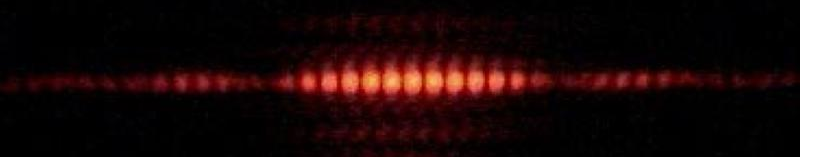
\includegraphics[scale=0.175,angle=90]{figures/Waves/fringes}};
%\clip (\w/2,-\d/2-\gap-\h) rectangle (\w/2+0.1,\d/2+\gap+\h);

}
\end{tikzpicture}
\captionof*{figure}{\textit{The interference pattern from light shining through two slits (double-slit experiment).}}
\end{center}
}
{
\capfig{1}{figures/Waves/veritassium}{Veritasium. Waves are created by two ball oscillating on top of the water. \url{https://www.youtube.com/watch?v=Iuv6hY6zsd0}}
}


%%%%%%%%%%%%%%%%%%%%%%%%%%%%%%%%
\subsubsection{Waves from two sources}
\label{subsubsec:wavesfromtwosources}
\begin{frame}{Waves from two sources}
\begin{center}
\animategraphics[autoplay,loop,width=10cm]{10}{figures/Waves/vwaves-}{0}{71}
\end{center}

\end{frame}


%%%%%%%%%%%%%%%%%%%%%%%%%%%%%%%%
\begin{frame}{Speakers interfering and beats}
\begin{center}

\begin{animateinline}[autoplay,loop]{10} % 5 fps, same as 0.2 s transduration

\multiframe{24}{i=1+1}{

\begin{tikzpicture}[scale=1]
\tikzmath{
\L=10;
\h=0.7;
\Ax1=0.75*\h;
\wl1=\L/40;%wavelength
\om1=2*pi/\wl1;%effective frequency
\Ax2=\Ax1;
\om2=1.05*\om1;%effective frequency
\phas=-2*pi/24*\i;
}
\scalebox{1}{

\draw[-latex,line width=1] (0,-\h) -- (0,1.2*\h) node[left]{$D_1$};
\draw[-latex,line width=1] (0,0) -- (1.05*\L,0) node[below]{$x$};

\draw[color=black!50] (0,-\h) grid[step=0.25] (\L,\h);
\draw[trig format=rad, line width=1,color=myblue!60] plot[ domain=0:\L, variable=\x, samples=700] ({\x},{\Ax1*sin(\om1*\x+\phas)});

\begin{scope}[shift={(0,-2.2*\h)}]
\draw[-latex,line width=1] (0,-\h) -- (0,1.2*\h) node[left]{$D_2$};
\draw[-latex,line width=1] (0,0) -- (1.05*\L,0) node[below]{$x$};
\draw[color=black!50] (0,-\h) grid[step=0.25] (\L,\h);
\draw[trig format=rad, line width=1,color=myblue!60] plot[ domain=0:\L, variable=\x, samples=700] ({\x},{\Ax2*sin(\om2*\x+\phas)});
\end{scope}

\begin{scope}[shift={(0,-5.9*\h)}]
\draw[-latex,line width=1] (0,-2.1*\h) -- (0,2.3*\h) node[left]{$D$};
\draw[-latex,line width=1] (0,0) -- (1.05*\L,0) node[below]{$x$};
\draw[color=black!50] (0,-2.1*\h) grid[step=0.25] (\L,2.1*\h);
\draw[trig format=rad, line width=1,color=myred] plot[ domain=0:\L, variable=\x, samples=700] ({\x},{\Ax1*sin(\om1*\x+\phas)+ \Ax2*sin(\om2*\x+\phas)});
\end{scope}

}
\end{tikzpicture}
}
\end{animateinline}
\captionof*{figure}{\textit{Waves with slightly different frequencies result in ``beats'' (here the frequencies are different by 5\%).}}
\end{center}
\end{frame}


%%%%%%%%%%%%%%%%%%%%%%%%%%%%%%%%
\subsection{Standing waves}
\label{subsec:standingwaves}
\begin{frame}{Standing waves}
\begin{itemize}
\item Particles in the medium are oscillating, but energy is not moving through the medium (as opposed to traveling waves).
\item This happens when waves traveling in opposite directions interfere, usually with their own reflections.
\item Examples:
\begin{itemize}
\item Vibrating guitar/piano/violin string.
\item Vibrating air inside an organ pipe.
\end{itemize}
\end{itemize}
\end{frame}


%%%%%%%%%%%%%%%%%%%%%%%%%%%%%%%%
\begin{frame}{Standing waves}
\begin{center}

\begin{animateinline}[autoplay,loop]{10} % 5 fps, same as 0.2 s transduration

\multiframe{48}{i=1+1}{

\begin{tikzpicture}[scale=1]
\tikzmath{
\L=8;
\h=0.7;
\Ax=0.75*\h;
\wl1=\L/6;%wavelength
\om1=2*pi/\wl1;%effective frequency
\phas=-2*pi/48*\i;
}
\scalebox{1}{

\useasboundingbox (-\L/4,-2.2*\Ax) rectangle (5*\L/4,2.2*\Ax);
\draw[trig format=rad, line width=1, color=myblue!60] plot[domain=0:5*\L/4, variable=\x, samples=100] ({\x},{\Ax*sin(\om1*\x-\phas)});
\draw[trig format=rad, line width=1, color=myblue!60] plot[domain=-\L/4:\L, variable=\x, samples=100] ({\x},{\Ax*sin(\om1*\x+\phas)});
\draw[trig format=rad, line width=1.5, color=myred] plot[domain=0:\L, variable=\x, samples=100] ({\x},{\Ax*sin(\om1*\x-\phas)+\Ax*sin(\om1*\x+\phas)});

}
\end{tikzpicture}
}
\end{animateinline}
\captionof*{figure}{\textit{Two traveling waves interfering to make a standing wave.}}
\end{center}



\begin{center}

\begin{animateinline}[autoplay,loop]{10} % 5 fps, same as 0.2 s transduration

\multiframe{48}{i=1+1}{

\begin{tikzpicture}[scale=1]
\tikzmath{
\L=8;
\h=0.7;
\Ax=0.75*\h;
\wl1=\L/3;%wavelength
\om1=2*pi/\wl1;%effective frequency
\phas=-2*pi/48*\i;
}
\scalebox{1}{

\useasboundingbox (-\L/4,-2.2*\Ax) rectangle (5*\L/4,2.2*\Ax);
\draw[trig format=rad, line width=1, color=myblue!60] plot[domain=0:5*\L/4, variable=\x, samples=100] ({\x},{\Ax*sin(\om1*\x-\phas)});
\draw[trig format=rad, line width=1, color=myblue!60] plot[domain=-\L/4:\L, variable=\x, samples=100] ({\x},{\Ax*sin(\om1*\x+\phas)});
\draw[trig format=rad, line width=1.5, color=myred] plot[domain=0:\L, variable=\x, samples=100] ({\x},{\Ax*sin(\om1*\x-\phas)+\Ax*sin(\om1*\x+\phas)});

}
\end{tikzpicture}
}
\end{animateinline}
\captionof*{figure}{\textit{Two different traveling waves interfering to make a standing wave.}}
\end{center}

\end{frame}

%%%%%%%%%%%%%%%%%%%%%%%%%%%%%%%%

%%%%%%%%%%%%%%%%%%%%%%%%%%%%%%%%
\subsubsection{Fundamentals and harmonics}
\label{subsubsec:fundamentalsandharmonics}
\twocolframesf{Standing waves: fundamentals and harmonics}
{
\begin{itemize}
\item We can characterize a standing wave by the number of nodes (don't move) and anti-nodes (max amplitude).
\item For a standing wave on a string, the ends are always nodes.
\end{itemize}
}
{
\begin{center}
\begin{tikzpicture}[scale=1]
\tikzmath{
\h=1.25;
\w=0.2;
\L=4;
\Ax=0.45*\h;
\wl1=2*\L;%wavelength
\om1=2*pi/\wl1;%effective frequency
\wl2=\L;
\om2=2*pi/\wl2;%effective frequency
\wl3=2*\L/3;
\om3=2*pi/\wl3;%effective frequency
}
\scalebox{1}{

\fill[color=myblue!60] (\L,-\h/2) rectangle +(\w,\h);
\node at (0,0) {
\includegraphics[scale=0.05,angle=-90]{figures/Waves/hand}};
\draw[dashed,brown,line width=1.5] (0,0) -- (\L,0);
\draw[trig format=rad, line width=1.5, color=brown] plot[ domain=0:\L, variable=\x, samples=100] ({\x},{\Ax*sin(\om1*\x)});
\draw[trig format=rad, line width=1.5, color=brown,dashed] plot[ domain=0:\L, variable=\x, samples=100] ({\x},{-\Ax*sin(\om1*\x)});

\begin{scope}[shift={(0,-1.1*\h)}]
\fill[color=myblue!60] (\L,-\h/2) rectangle +(\w,\h);
\node at (0,0) {
\includegraphics[scale=0.05,angle=-90]{figures/Waves/hand}};
\draw[dashed,brown,line width=1.5] (0,0) -- (\L,0);
\draw[trig format=rad, line width=1.5, color=brown] plot[ domain=0:\L, variable=\x, samples=100] ({\x},{\Ax*sin(\om2*\x)});
\draw[trig format=rad, line width=1.5, color=brown,dashed] plot[ domain=0:\L, variable=\x, samples=100] ({\x},{-\Ax*sin(\om2*\x)});
\end{scope}

\begin{scope}[shift={(0,-2.2*\h)}]
\fill[color=myblue!60] (\L,-\h/2) rectangle +(\w,\h);
\node at (0,0) {
\includegraphics[scale=0.05,angle=-90]{figures/Waves/hand}};
\draw[dashed,brown,line width=1.5] (0,0) -- (\L,0);
\draw[trig format=rad, line width=1.5, color=brown] plot[ domain=0:\L, variable=\x, samples=100] ({\x},{\Ax*sin(\om3*\x)});
\draw[trig format=rad, line width=1.5, color=brown,dashed] plot[ domain=0:\L, variable=\x, samples=100] ({\x},{-\Ax*sin(\om3*\x)});

\end{scope}


}
\end{tikzpicture}
\captionof*{figure}{\textit{The first 3 harmonics (fundamental, first overtone, second overtone).}}
\end{center}
}


%%%%%%%%%%%%%%%%%%%%%%%%%%%%%%%%
\subsubsection{Resonance}
\label{subsubsec:resonance}
\begin{frame}{Standing waves and resonance}
\begin{itemize}
\item We can think of objects as having ``resonant frequencies'' that correspond to the frequencies (wavelengths) of the fundamental frequency and the harmonics.
\item If you make an object vibrate, most of the waves will destructively interfere, but the waves at the right frequencies can setup standing waves that can become quite large. 
\item You don't need to shake the end of the object at a particular frequency to create a standing wave inside of it. 
\item If you pluck a guitar string, you effectively send a bunch of sine waves along the string; those that correspond to the harmonics will constructively interfere and dominate the sound that you hear.
\end{itemize}
\end{frame}


%%%%%%%%%%%%%%%%%%%%%%%%%%%%%%%%



%%%%%%%%%%%%%%%%%%%%%%%%%%%%%%%%


%%%%%%%%%%%%%%%%%%%%%%%%%%%%%%%%


%%%%%%%%%%%%%%%%%%%%%%%%%%%%%%%%
\twocolframe{Description of a standing wave}
{
\begin{itemize}
\item In contrast to a traveling wave, in a standing wave, each point oscillates with a different amplitude.
\item We can describe each point on the string with:
\begin{align*}
D(x,t)=2A\sin\left(\frac{n\pi}{L}x\right) \cos(\omega t)
\end{align*}
\item Each point oscillates as a simple harmonic oscillator:
\begin{align*}
D(x,t)=A(x)\cos(\omega t)
\end{align*}
\end{itemize}
}
{
\begin{center}
\begin{tikzpicture}[scale=1]
\tikzmath{
\h=1.25;
\w=0.2;
\L=4;
\Ax=0.45*\h;
\wl1=2*\L;%wavelength
\om1=2*pi/\wl1;%effective frequency
\wl2=\L;
\om2=2*pi/\wl2;%effective frequency
\wl3=2*\L/3;
\om3=2*pi/\wl3;%effective frequency
}
\scalebox{1}{

\fill[color=myblue!60] (\L,-\h/2) rectangle +(\w,\h);
\node at (0,0) {
\includegraphics[scale=0.05,angle=-90]{figures/Waves/hand}};
\draw[dashed,brown,line width=1.5] (0,0) -- (\L,0);
\draw[trig format=rad, line width=1.5, color=brown] plot[ domain=0:\L, variable=\x, samples=100] ({\x},{\Ax*sin(\om1*\x)});
\draw[trig format=rad, line width=1.5, color=brown,dashed] plot[ domain=0:\L, variable=\x, samples=100] ({\x},{-\Ax*sin(\om1*\x)});

\begin{scope}[shift={(0,-1.1*\h)}]
\fill[color=myblue!60] (\L,-\h/2) rectangle +(\w,\h);
\node at (0,0) {
\includegraphics[scale=0.05,angle=-90]{figures/Waves/hand}};
\draw[dashed,brown,line width=1.5] (0,0) -- (\L,0);
\draw[trig format=rad, line width=1.5, color=brown] plot[ domain=0:\L, variable=\x, samples=100] ({\x},{\Ax*sin(\om2*\x)});
\draw[trig format=rad, line width=1.5, color=brown,dashed] plot[ domain=0:\L, variable=\x, samples=100] ({\x},{-\Ax*sin(\om2*\x)});
\end{scope}

\begin{scope}[shift={(0,-2.2*\h)}]
\fill[color=myblue!60] (\L,-\h/2) rectangle +(\w,\h);
\node at (0,0) {
\includegraphics[scale=0.05,angle=-90]{figures/Waves/hand}};
\draw[dashed,brown,line width=1.5] (0,0) -- (\L,0);
\draw[trig format=rad, line width=1.5, color=brown] plot[ domain=0:\L, variable=\x, samples=100] ({\x},{\Ax*sin(\om3*\x)});
\draw[trig format=rad, line width=1.5, color=brown,dashed] plot[ domain=0:\L, variable=\x, samples=100] ({\x},{-\Ax*sin(\om3*\x)});

\end{scope}


}
\end{tikzpicture}
\captionof*{figure}{\textit{The first 3 harmonics (fundamental, first overtone, second overtone).}}
\end{center}
}

%%%%%%%%%%%%%%%%%%%%%%%%%%%%%%%%































%%%%%%%%%%%%%%%%%%%%%%%%%%%%%%%%

\title{Fluid Mechanics}
\subject{Pressure, Hydrostatics/Dynamics and Bernoulli's Principle}
\subtitle{Building Models to Describe our World}


%%%%%%%%%%%%%%%%%%%%%%%%%
%%%%%% Title slide %%%%%%
%%%%%%%%%%%%%%%%%%%%%%%%%
\chaptertitle{Fluid Mechanics}
\begin{frame}
\label{chap:fluidmechanics}
\titlepage
\thispagestyle{empty}

\begin{textblock*}{5cm}(11cm,4cm)
    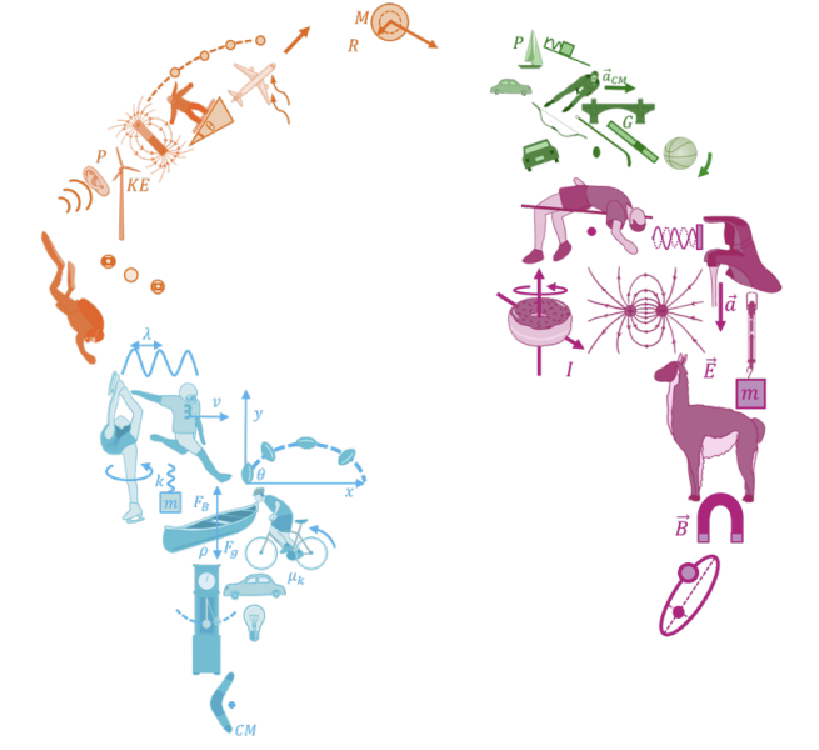
\includegraphics[width=4cm]{figures/BMDW/logo}
\end{textblock*}

\end{frame}

%%%%%%%%%%%%%%%%%%%%%%%%%%%%%%%%
%%Advertisements and such %%%%%%
%%%%%%%%%%%%%%%%%%%%%%%%%%%%%%%%

\twocolframe{Outline}
  {\tableofcontents[sections={40,41}, subsectionstyle=show/show]\thispagestyle{empty}}
  {\tableofcontents[sections={42}, subsectionstyle=show/show]}



%%%%%%%%%%%%%%%%%%%%%%%%%%%%%%%%%%%%%%%%%%%%%%%%%%%%%%%%%%%%%%
%% Annoucements                                         %%%%%%
%%%%%%%%%%%%%%%%%%%%%%%%%%%%%%%%%%%%%%%%%%%%%%%%%%%%%%%%%%%%%%

%%%%%%%%%%%%%%%%%%%%%%%%%%%%%%


\section{Pressure}
\label{sec:pressure}
\title{Pressure}


%%%%%%%%%%%%%%%%%%%%%%%%%
\begin{frame}
\titlepage
\thispagestyle{empty}
\end{frame}


%%%%%%%%%%%%%%%%%%%%%%%%%%%%%%%%%%%%%%%%%%%%%%%%%%%%%%%%%%%%%%%%%%%%%%%%%%%%%%%%%%%%%%%

\begin{frame}{Pressure}
\begin{itemize}
\item Defined as force per unit area:
\begin{align*}
P=\frac{F}{A}
\end{align*}
\item Scalar quantity.
\item Exerts a force that is normal to any surface.
\end{itemize}

\end{frame}


%%%%%%%%%%%%%%%%%%%%%%%%%%%%%%%%


%%%%%%%%%%%%%%%%%%%%%%%%%%%%%%%%
\subsection{Pressure in a fluid}
\label{subsec:pressureinafluid}
\twocolframesf{Pressure in a fluid}
{
\begin{itemize}
\item Pressure is a scalar, it does not have a direction.
\item A fluid (liquid or gas) cannot transmit force in a particular direction.
\item The pressure in a fluid is in all directions.
\item If there is a boundary on the fluid (e.g. a container), then the force from the pressure in the fluid is normal to the surface
\item You can think of the particles in the fluid as bouncing against the surfaces. The force required to change their momentum is the reaction force to the force associated with their pressure.
\end{itemize}
}
{

\begin{center}
\begin{tikzpicture}[scale=1]
\tikzmath{
\L=4;
}
\scalebox{1}{

\draw[line width=2] (0,0) rectangle (\L,\L);

\foreach \i in {0,...,30}{
\tikzmath{
\xpos = 0.35*(1.3+rand)*\L;
\ypos = 0.35*(1.3+rand)*\L;
\th = 0.5*(1+rand)*360;
}
%\draw[color=black!50,line width=2pt] (\xpos,\ypos) -- +(\th:0.25);
\begin{scope}[shift={(\xpos,\ypos)}, rotate=\th]
\foreach \j in {1,...,5}{
\tikzmath{
 \xs=\j*0.075;
 \tra=\j*0.2;
}
\shade[ball color=black, opacity=\tra] (\xs,0)  circle (2pt);
}
\end{scope}
}

\coordinate (P1) at (0,3*\L/4);
\shade[ball color=myred, opacity=0.2] ($(P1)+(45:0.375)$) circle (2pt);
\shade[ball color=myred, opacity=0.3] ($(P1)+(45:0.30)$) circle (2pt);
\shade[ball color=myred, opacity=0.4] ($(P1)+(45:0.225)$) circle (2pt);
\shade[ball color=myred, opacity=0.5] ($(P1)+(45:0.15)$) circle (2pt);
\shade[ball color=myred, opacity=0.6] ($(P1)+(0.05,0)$) circle (2pt);
\shade[ball color=myred, opacity=0.7] ($(P1)+(-45:0.15)$) circle (2pt);
\shade[ball color=myred, opacity=0.8] ($(P1)+(-45:0.225)$) circle (2pt);
\shade[ball color=myred, opacity=0.9] ($(P1)+(-45:0.30)$) circle (2pt);
\shade[ball color=myred, opacity=1] ($(P1)+(-45:0.375)$) circle (2pt);
\draw[-latex, color=myred, line width=1.5] (P1) -- +(-0.5,0);

\coordinate (P1b) at (0,\L/4);
\shade[ball color=myred, opacity=0.2] ($(P1b)+(45:0.375)$) circle (2pt);
\shade[ball color=myred, opacity=0.3] ($(P1b)+(45:0.30)$) circle (2pt);
\shade[ball color=myred, opacity=0.4] ($(P1b)+(45:0.225)$) circle (2pt);
\shade[ball color=myred, opacity=0.5] ($(P1b)+(45:0.15)$) circle (2pt);
\shade[ball color=myred, opacity=0.6] ($(P1b)+(0.05,0)$) circle (2pt);
\shade[ball color=myred, opacity=0.7] ($(P1b)+(-45:0.15)$) circle (2pt);
\shade[ball color=myred, opacity=0.8] ($(P1b)+(-45:0.225)$) circle (2pt);
\shade[ball color=myred, opacity=0.9] ($(P1b)+(-45:0.30)$) circle (2pt);
\shade[ball color=myred, opacity=1] ($(P1b)+(-45:0.375)$) circle (2pt);
\draw[-latex, color=myred, line width=1.5] (P1b) -- +(-0.5,0);

\coordinate (P2) at (\L,\L/4);
\shade[ball color=myred, opacity=0.2] ($(P2)+(135:0.375)$) circle (2pt);
\shade[ball color=myred, opacity=0.3] ($(P2)+(135:0.30)$) circle (2pt);
\shade[ball color=myred, opacity=0.4] ($(P2)+(135:0.225)$) circle (2pt);
\shade[ball color=myred, opacity=0.5] ($(P2)+(135:0.15)$) circle (2pt);
\shade[ball color=myred, opacity=0.6] ($(P2)+(-0.05,0)$) circle (2pt);
\shade[ball color=myred, opacity=0.7] ($(P2)+(225:0.15)$) circle (2pt);
\shade[ball color=myred, opacity=0.8] ($(P2)+(225:0.225)$) circle (2pt);
\shade[ball color=myred, opacity=0.9] ($(P2)+(225:0.30)$) circle (2pt);
\shade[ball color=myred, opacity=1] ($(P2)+(225:0.375)$) circle (2pt);
\draw[-latex, color=myred, line width=1.5] (P2) -- +(0.5,0);

\coordinate (P2b) at (\L,3*\L/4);
\shade[ball color=myred, opacity=0.2] ($(P2b)+(135:0.375)$) circle (2pt);
\shade[ball color=myred, opacity=0.3] ($(P2b)+(135:0.30)$) circle (2pt);
\shade[ball color=myred, opacity=0.4] ($(P2b)+(135:0.225)$) circle (2pt);
\shade[ball color=myred, opacity=0.5] ($(P2b)+(135:0.15)$) circle (2pt);
\shade[ball color=myred, opacity=0.6] ($(P2b)+(-0.05,0)$) circle (2pt);
\shade[ball color=myred, opacity=0.7] ($(P2b)+(225:0.15)$) circle (2pt);
\shade[ball color=myred, opacity=0.8] ($(P2b)+(225:0.225)$) circle (2pt);
\shade[ball color=myred, opacity=0.9] ($(P2b)+(225:0.30)$) circle (2pt);
\shade[ball color=myred, opacity=1] ($(P2b)+(225:0.375)$) circle (2pt);
\draw[-latex, color=myred, line width=1.5] (P2b) -- +(0.5,0);

\coordinate (P3) at (3*\L/4,\L);
\shade[ball color=myred, opacity=0.2] ($(P3)+(-45:0.375)$) circle (2pt);
\shade[ball color=myred, opacity=0.3] ($(P3)+(-45:0.30)$) circle (2pt);
\shade[ball color=myred, opacity=0.4] ($(P3)+(-45:0.225)$) circle (2pt);
\shade[ball color=myred, opacity=0.5] ($(P3)+(-45:0.15)$) circle (2pt);
\shade[ball color=myred, opacity=0.6] ($(P3)+(0,-0.05)$) circle (2pt);
\shade[ball color=myred, opacity=0.7] ($(P3)+(225:0.15)$) circle (2pt);
\shade[ball color=myred, opacity=0.8] ($(P3)+(225:0.225)$) circle (2pt);
\shade[ball color=myred, opacity=0.9] ($(P3)+(225:0.30)$) circle (2pt);
\shade[ball color=myred, opacity=1] ($(P3)+(225:0.375)$) circle (2pt);
\draw[-latex, color=myred, line width=1.5] (P3) -- +(0,0.5);

\coordinate (P3b) at (\L/4,\L);
\shade[ball color=myred, opacity=0.2] ($(P3b)+(-45:0.375)$) circle (2pt);
\shade[ball color=myred, opacity=0.3] ($(P3b)+(-45:0.30)$) circle (2pt);
\shade[ball color=myred, opacity=0.4] ($(P3b)+(-45:0.225)$) circle (2pt);
\shade[ball color=myred, opacity=0.5] ($(P3b)+(-45:0.15)$) circle (2pt);
\shade[ball color=myred, opacity=0.6] ($(P3b)+(0,-0.05)$) circle (2pt);
\shade[ball color=myred, opacity=0.7] ($(P3b)+(225:0.15)$) circle (2pt);
\shade[ball color=myred, opacity=0.8] ($(P3b)+(225:0.225)$) circle (2pt);
\shade[ball color=myred, opacity=0.9] ($(P3b)+(225:0.30)$) circle (2pt);
\shade[ball color=myred, opacity=1] ($(P3b)+(225:0.375)$) circle (2pt);
\draw[-latex, color=myred, line width=1.5] (P3b) -- +(0,0.5);

\coordinate (P4) at (\L/4,0);
\shade[ball color=myred, opacity=0.2] ($(P4)+(135:0.375)$) circle (2pt);
\shade[ball color=myred, opacity=0.3] ($(P4)+(135:0.30)$) circle (2pt);
\shade[ball color=myred, opacity=0.4] ($(P4)+(135:0.225)$) circle (2pt);
\shade[ball color=myred, opacity=0.5] ($(P4)+(135:0.15)$) circle (2pt);
\shade[ball color=myred, opacity=0.6] ($(P4)+(0,0.05)$) circle (2pt);
\shade[ball color=myred, opacity=0.7] ($(P4)+(45:0.15)$) circle (2pt);
\shade[ball color=myred, opacity=0.8] ($(P4)+(45:0.225)$) circle (2pt);
\shade[ball color=myred, opacity=0.9] ($(P4)+(45:0.30)$) circle (2pt);
\shade[ball color=myred, opacity=1] ($(P4)+(45:0.375)$) circle (2pt);
\draw[-latex, color=myred, line width=1.5] (P4) -- +(0,-0.5);

\coordinate (P4b) at (3*\L/4,0);
\shade[ball color=myred, opacity=0.2] ($(P4b)+(135:0.375)$) circle (2pt);
\shade[ball color=myred, opacity=0.3] ($(P4b)+(135:0.30)$) circle (2pt);
\shade[ball color=myred, opacity=0.4] ($(P4b)+(135:0.225)$) circle (2pt);
\shade[ball color=myred, opacity=0.5] ($(P4b)+(135:0.15)$) circle (2pt);
\shade[ball color=myred, opacity=0.6] ($(P4b)+(0,0.05)$) circle (2pt);
\shade[ball color=myred, opacity=0.7] ($(P4b)+(45:0.15)$) circle (2pt);
\shade[ball color=myred, opacity=0.8] ($(P4b)+(45:0.225)$) circle (2pt);
\shade[ball color=myred, opacity=0.9] ($(P4b)+(45:0.30)$) circle (2pt);
\shade[ball color=myred, opacity=1] ($(P4b)+(45:0.375)$) circle (2pt);
\draw[-latex, color=myred, line width=1.5] (P4b) -- +(0,-0.5);
}

\end{tikzpicture}
\captionof*{figure}{\textit{Particles in the fluid bounce against the boundaries exerting an outward normal force.}}
\end{center}

}


%%%%%%%%%%%%%%%%%%%%%%%%%%%%%%%%



%%%%%%%%%%%%%%%%%%%%%%%%%%%%%%%%
\subsection{Equilibirem}
\label{subsec:equilibriem}
\twocolframesf{Hydrostatic equilibrium}
{
\begin{itemize}
\item Literally: Water not move equilibrium.
\item Think of an element of fluid that is not moving.
\end{itemize}
}
{
\begin{center}
\begin{tikzpicture}[scale=1]
\tikzmath{
\L=4;
\abox=0.75;
}
\scalebox{1}{

\fill[color=cyan!50] (-\L/2,-\L/2) rectangle (\L/2,\L/2);
\draw[line width=1] (-\abox/2,-\abox/2) rectangle (\abox/2,\abox/2);

\draw[latex-, line width=1.5] (-\abox/2,-\abox/2) -- +(225:0.75);
\draw[latex-, line width=1.5] (\abox/2,-\abox/2) -- +(-45:0.75);
\draw[latex-, line width=1.5] (\abox/2,\abox/2) -- +(45:0.75);
\draw[latex-, line width=1.5] (-\abox/2,\abox/2) -- +(135:0.75);

\draw[latex-, line width=1.5] (0,\abox/2) -- +(90:0.75);
\draw[latex-, line width=1.5] (0,-\abox/2) -- +(-90:0.75);
\draw[latex-, line width=1.5] (\abox/2,0) -- +(0:0.75);
\draw[latex-, line width=1.5] (-\abox/2,0) -- +(180:0.75);
}

\end{tikzpicture}
\captionof*{figure}{\textit{A fluid element in hydrostatic equilibrium.}}
\end{center}
}


%%%%%%%%%%%%%%%%%%%%%%%%%%%%%%%%
\subsection{Pressure gradient}
\label{subsec:prssuregradient}
\twocolframesf{Pressure gradient in a fluid}
{
\begin{itemize}
\item In order for the fluid element to be in equilibrium, the net force on it must be zero:
\begin{align*}
\sum F_y=P_2A -mg- P_1A=0
\end{align*}
\item Using density for the mass:
\begin{align*}
m=\rho V = \rho A h
\end{align*}
\item Altogether:
\begin{align*}
P_2A -\rho A hg- P_1A&=0\\
P_2-P_1=\rho g h
\end{align*}

\end{itemize}
}
{
\vspace{-1.5cm}
\begin{center}
\begin{tikzpicture}[scale=1]
\tikzmath{
\L=4;
\abox=1;
}
\scalebox{1}{

\fill[color=cyan!50] (-\L/2,-\L/2) rectangle (\L/2,\L/2);

\draw[line width=1] (-0.4*\L,-\abox/2) rectangle (0.4*\L,\abox/2);


\foreach \xp in {-0.3,-0.2,-0.1,...,0.3}{
\draw[latex-,line width=1.5] (\xp*\L,\abox/2) -- +(0,0.5);
\draw[latex-,line width=1.5] (\xp*\L,-\abox/2) -- +(0,-0.75);
}

\draw[-latex, line width=1] (0.75*\L,-\L/2) -- +(0,\L) node[left]{$y$};
\draw[-latex, line width=2] (0.65*\L,\abox/2) -- +(0,-1) node[midway, left]{$\vec g$};

\draw[latex-latex] (0.25*\L,-\abox/2) --(0.25*\L, \abox/2) node[midway, right]{$h$};

\node[above] at (0,-\abox/2) {$A_2$};
\node[below] at (0,\abox/2) {$A_1$};


\node[above] at (0,-2*\abox) {$P_2$};
\node[below] at (0,1.5*\abox) {$P_1$};
}

\end{tikzpicture}
\captionof*{figure}{\textit{A fluid element in hydrostatic equilibrium, with gravity.}}
\end{center}

\only<2>{
In other words, the pressure increases as you move down:
\begin{align*}
P_2=P_1+\rho g h
\end{align*}
}
}


%%%%%%%%%%%%%%%%%%%%%%%%%%%%%%%%

\twocolframesf{If the fluid is \textit{compressible}}
{
\begin{itemize}
\item The density of the fluid can vary with pressure (e.g. if the fluid is a gas, like the Earth's atmosphere).
\item Then, we model an infinitesimal fluid element, small enough so that density is constant:
\begin{align*}
\frac{dP}{dy}&=-\rho g\\
\therefore P(y_2)-P(y_1)&= \int_{y_1}^{y_2} \rho(y) g dy
\end{align*}
\item For constant density, recover:
\begin{align*}
\int_{y_1}^{y_2} \rho(y) g dy = \rho g (y_2-y_1) = \rho g h
\end{align*}

\end{itemize}
}
{
\begin{center}
\begin{tikzpicture}[scale=1]
\tikzmath{
\L=4;
\abox=0.5;
}
\scalebox{1}{

\fill[color=cyan!50] (-\L/2,-\L/2) rectangle (\L/2,\L/2);

\draw[line width=1] (-0.35*\L,-\abox/2) rectangle (0.35*\L,\abox/2);


\foreach \xp in {-0.3,-0.2,-0.1,...,0.3}{
\draw[latex-,line width=1.5] (\xp*\L,\abox/2) -- +(0,0.5);
\draw[latex-,line width=1.5] (\xp*\L,-\abox/2) -- +(0,-0.75);
}

\draw[-latex, line width=1] (0.75*\L,-\L/2) -- +(0,\L) node[left]{$y$};
\draw[-latex, line width=2] (0.65*\L,\abox/2) -- +(0,-1) node[midway, left]{$\vec g$};

\draw[latex-latex] (0.375*\L,-\abox/2) --(0.375*\L, \abox/2) node[midway, right]{$dy$};

\node[above] at (0,1) {$P+dP$};
\node[below] at (0,-1.25) {$P$};
}

\end{tikzpicture}
\captionof*{figure}{\textit{A compressible fluid element in hydrostatic equilibrium. Note that $dP$ is negative in the figure.}}
\end{center}

}



%%%%%%%%%%%%%%%%%%%%%%%%%%%%%%%%
\subsection{Atmospheric pressure}
\begin{frame}{The Earth's atmosphere}
\begin{itemize}
\item A rough approximation is that density is proportional to pressure (e.g. ideal gas law).
\begin{align*}
\rho(y) = a P(y)
\end{align*}
where $a$ is just a constant of proportionality.

\item One finds that:
\begin{align*}
\frac{dP}{dy}&=-\rho g=-a P(y) g\\
\therefore P(y) &= P_0 e^{-agy}
\end{align*}

\item Pressure decreases exponentially with increasing altitude.
\end{itemize}
\end{frame}


%%%%%%%%%%%%%%%%%%%%%%%%%%%%%%%%
\subsection{Pascal's principle}
\label{subsec:pascalsprinciple}
\twocolframesf{Pascal’s principle}
{
\begin{itemize}
\item If you exert an external pressure on a fluid, the pressure in the fluid increases everywhere by the same amount.
\item<2-> The absolute pressure in, say, water, then depends on the atmospheric pressure, $P_0$:
\begin{align*}
P_2=P_0+P_1+\rho g h
\end{align*}
\item<2-> Or, in general, some distance $h$ below the surface:
\begin{align*}
P_2=P_0+\rho g h
\end{align*}
\end{itemize}
}
{
\only<1>{
\begin{center}
\begin{tikzpicture}[scale=1]
\tikzmath{
\abox=2;
}
\scalebox{1}{
\fill[color=cyan!50] (0,0) rectangle (\abox/2,\abox);
\draw[line width=1] (-\abox,0) rectangle (\abox/2,\abox);
\fill(-0.25*\abox,0) rectangle (0,\abox);
\fill(-1.25*\abox,0.4*\abox) rectangle (-0.25*\abox,0.6*\abox);
\draw[latex-, line width=1.5] (-1.25*\abox,0.5*\abox) -- +(-1,0) node[midway,above]{$\vec F$};
\node[right] at (0,\abox/2) {$A$};
}

\end{tikzpicture}
\captionof*{figure}{\textit{Pascal's principle: applying pressure externally to a fluid increases its pressure.}}
\end{center}
}

\only<2->{
\begin{center}
\begin{tikzpicture}[scale=1]
\tikzmath{
\L=4;
\abox=1;
}
\scalebox{1}{

\fill[color=cyan!50] (-\L/2,-\L/2) rectangle (\L/2,\L/2);

\draw[line width=1] (-0.4*\L,-\abox/2) rectangle (0.4*\L,\abox/2);

\foreach \xp in {-0.4,-0.2,0,...,0.4}{
\draw[latex-,line width=1.5] (\xp*\L,\L/2) -- +(0,0.75);
}
\node[right] at (0,2.5) {$P_0$};

\foreach \xp in {-0.3,-0.2,-0.1,...,0.3}{
\draw[latex-,line width=1.5] (\xp*\L,\abox/2) -- +(0,0.5);
\draw[latex-,line width=1.5] (\xp*\L,-\abox/2) -- +(0,-0.75);
}

\draw[-latex, line width=1] (0.75*\L,-\L/2) -- +(0,\L) node[left]{$y$};
\draw[-latex, line width=2] (0.65*\L,\abox/2) -- +(0,-1) node[midway, left]{$\vec g$};

\draw[latex-latex] (0.25*\L,-\abox/2) --(0.25*\L, \abox/2) node[midway, right]{$h$};

\node[above] at (0,-2*\abox) {$P_2$};
\node[below] at (0,1.5*\abox) {$P_1$};
}

\end{tikzpicture}
\captionof*{figure}{\textit{A fluid with atmospheric pressure on it.}}
\end{center}
}

}


%%%%%%%%%%%%%%%%%%%%%%%%%%%%%%%%



%%%%%%%%%%%%%%%%%%%%%%%%%%%%%%%%



%%%%%%%%%%%%%%%%%%%%%%%%%%%%%%%%



%%%%%%%%%%%%%%%%%%%%%%%%%%%%%%%%

\section{Hydrostatics/Dynamics}
\label{sec:hydrostaticsdynamics}
\title{Hydrostatics and Dynamics}


%%%%%%%%%%%%%%%%%%%%%%%%%
\begin{frame}
\titlepage
\thispagestyle{empty}
\end{frame}

%%%%%%%%%%%%%%%%%%%%%%%%%%%%%%%%



%%%%%%%%%%%%%%%%%%%%%%%%%%%%%%%%
\subsection{Buoyancy}
\label{subsec:buoyancy}
\twocolframe{Buoyancy}
{
\vspace{-0.25cm}
\begin{itemize}
\item Same effect as hydrostatic equilibrium.
\item There is a net upwards force on the fluid element because of the pressure gradient (due to gravity – pressure increases downwards).
\item If you replace the fluid element with an object, that pressure gradient and resulting upwards force does not go away!
\item Magnitude of the force is equal to the weight of the fluid displaced:
\begin{align*}
F_B=m_{fluid}g=\rho V g
\end{align*}
\item This does not change with depth!
\end{itemize}
}
{
\vspace{-0.75cm}
\begin{center}
\begin{tikzpicture}[scale=1]
\tikzmath{
\L=4;
\R=1;
}
\scalebox{1}{

\fill[color=cyan!50] (-\L/2,-\L/2) rectangle (\L/2,0);
\draw[line width =1.5] (-\L/2,0) -- (-\L/2,-\L/2)  -- (\L/2,-\L/2) -- (\L/2,0);

\draw[line width=1.5, dashed] (-\R,0) -- (\R,0) arc(0:-180:\R);
\coordinate (P1) at (0,-\R/2);
\fill (P1) circle(2pt);
\draw[-latex, line width=1.5] (P1) -- +(0,1) node[left]{$\vec F_B$};
\draw[-latex, line width=1.5] (P1) -- +(0,-1) node[left]{$\vec F_g$};
\node[left] at  (0,-\R/2){$V$};

\foreach \th in {210,240,300, 330}{
 \draw[latex-,line width=1] (\th:\R) -- +(\th:0.7);
}

\begin{scope}[shift={(0,-0.75*\L)}]
\fill[color=cyan!50] (-\L/2,-\L/2) rectangle (\L/2,0);
\draw[line width =1.5] (-\L/2,0) -- (-\L/2,-\L/2)  -- (\L/2,-\L/2) -- (\L/2,0);

\draw[line width=1.5, dashed, fill=brown] (-\R,0) -- (\R,0) arc(0:-180:\R)--cycle;
\coordinate (P1) at (0,-\R/2);
\fill (P1) circle(2pt);
\draw[-latex, line width=1.5] (P1) -- +(0,1) node[left]{$\vec F_B$};


\foreach \th in {210,240,300,270,330}{
 \draw[latex-,line width=1] (\th:\R) -- +(\th:0.7);
}
\end{scope}

}

\end{tikzpicture}
\captionof*{figure}{\textit{A volume, $V$, supported by the same buoyancy force, regardless of being filled by fluid or an object.}}
\end{center}
}


%%%%%%%%%%%%%%%%%%%%%%%%%%%%%%%%



%%%%%%%%%%%%%%%%%%%%%%%%%%%%%%%%


%%%%%%%%%%%%%%%%%%%%%%%%%%%%%%%%
\subsection{Origin of buoyancy force}
\label{subsec:originofbuoyancyforce}
\twocolframesf{Buoyancy force comes from pressure gradient}
{
\begin{itemize}
\item At rest, there is a pressure gradient in the air that is downwards because of gravity.
\item When the car is accelerating, each element of the air must also accelerate with the car:
\begin{itemize}
\item The sum of the forces must be:
\begin{align*}
\sum F = ma =\rho V a
\end{align*}
\item The only way this can happen is if the pressure gradient is in a direction to accelerate the fluid with the car (must oppose gravity and go to the right).
\end{itemize}

\end{itemize}
}
{
\vspace{-0.5cm}
\begin{center}
\begin{tikzpicture}[scale=1]
\tikzmath{
\L=3.5;
\abox=0.5;
}
\scalebox{1}{

\fill[color=cyan!50] (-\L/2,-\L/2) rectangle (\L/2,0);
\draw[line width =1.5] (-\L/2,\L/4) -- (-\L/2,-\L/2)  -- (\L/2,-\L/2) -- (\L/2,\L/4) --cycle;

\draw[line width =1] (-0.75*\L/2,-\L/4-\abox/2) rectangle +(\abox,\abox);
\coordinate (P) at ($ (-0.75*\L/2,-\L/4-\abox/2) +(\abox/2,\abox/2)$);
\fill (P) circle (2pt);
\draw[-latex, line width =1] (P) -- +(0,0.75) node[right]{\scriptsize $\vec F_B$};
\draw[-latex, line width =1] (P) -- +(0,-0.75) node[above right]{\scriptsize $\vec F_g$};

\draw[line width =2] (0,-\L/2) -- +(0,0.75);
\fill[color=myred] ($ (0, -\L/2)+(0,0.75)+(0,0.25) $) circle(0.25);

\begin{scope}[shift={(0,-0.95*\L)}]
\fill[color=cyan!50] (-\L/2,0.35) -- (-\L/2,-\L/2)  -- (\L/2,-\L/2) -- (\L/2,-0.25) --cycle;
\draw[line width =1.5] (-\L/2,\L/4) -- (-\L/2,-\L/2)  -- (\L/2,-\L/2) -- (\L/2,\L/4) --cycle;

\draw[line width =1] (-0.75*\L/2,-\L/4-\abox/2) rectangle +(\abox,\abox);
\coordinate (P) at ($ (-0.75*\L/2,-\L/4-\abox/2) +(\abox/2,\abox/2)$);
\fill (P) circle (2pt);
\draw[-latex, line width =1] (P) -- +(70:0.75) node[right]{\scriptsize $\vec F_B$};
\draw[-latex, line width =1] (P) -- +(0,-0.75) node[above right]{\scriptsize $\vec F_g$};

\draw[line width =2] (0,-\L/2) -- +(70:0.75);
\fill[color=myred] ($ (0, -\L/2)+(70:0.75)+(70:0.25) $) circle(0.25);

\draw[-latex,line width=2] (\L/4,0.75*\L/4) -- +(0.75,0) node[midway,below]{$\vec a$};

\coordinate (P) at (1.5*\L/2,-\L/8);
\fill (P) circle (3pt);
\draw[-latex, line width=1.5] (P) --+(0,-1) node[right]{$\vec F_g$};
\draw[-latex, line width=1.5] (P) --+(250:0.75) node[left]{$\vec T$};
\draw[-latex, line width=1.5] (P) --+(70:1.5) node[above]{$\vec F_B$};
\end{scope}


}

\end{tikzpicture}
\captionof*{figure}{\textit{A fluid accelerating in a container with a floating ballon. FBD of forces on balloon.}}
\end{center}
}


%%%%%%%%%%%%%%%%%%%%%%%%%%%%%%%%
\subsection{Hydrodynamics - flow rate}
\twocolframesf{Hydrodynamics - Flow rate, $Q$}
{
\begin{itemize}
\item Think of liquid moving through a horizontal pipe of cross section, $A$.
\item Continuity:
\begin{itemize}
\item What comes in must come out!
\item If we put in \SI{10}{l/min} into a pipe, then \SI{10}{l/min} must come out the other end (incompressible)
\end{itemize}
\item If the liquid flows at a speed, $v$, it covers a distance, $\Delta x$ in a time, $\Delta t$.  
\item The volume of fluid flowing per unit time is called the flow rate:
\begin{align*}
Q=\frac{\Delta V}{\Delta t}=\frac{\Delta x A}{\Delta t}=Av
\end{align*}
\end{itemize}
}
{
\begin{center}
\begin{tikzpicture}[scale=1]
\tikzmath{
\L=5;
\R=0.75;
}
\scalebox{1}{

\fill[top color=myblue!20, bottom color=myblue!40] (0,\R) -- (\L,\R) arc (90:-90:\R/4 and \R) -- (0,-\R) arc(-90:90:\R/4 and \R);
\fill[top color=myblue!40, bottom color=myblue!60, draw=black]  (0,0) circle (\R/4 and \R);

\fill[top color=myblue!60, bottom color=myblue!80] (0.4*\L,\R) -- (0.6*\L,\R) arc (90:-90:\R/4 and \R) -- (0.4*\L,-\R) arc(-90:90:\R/4 and \R);
\fill[top color=myblue!80, bottom color=myblue!90]  (0.4*\L,0) circle (\R/4 and \R);
\draw[line width=1, dotted]  (0.6*\L,\R) arc (90:270:\R/4 and \R);
\draw[line width=1]  (0.6*\L,\R) arc (90:-90:\R/4 and \R);

\draw[-latex,line width=1.5]  (0.6*\L,0)--+(1,0) node[below]{$\vec v$};
\node[color=white] at (\L/2,0) {$\Delta V$};
\draw[latex-latex] (0.4*\L,\R+0.1) -- (0.6*\L,\R+0.1) node[midway,above]{$\Delta x$};
\node[left] at (-0.2,0) {$A$};
}

\end{tikzpicture}
\captionof*{figure}{\textit{A fluid element, of volume, $\Delta v$, moving in a pipe.}}
\end{center}
}


%%%%%%%%%%%%%%%%%%%%%%%%%%%%%%%%


%%%%%%%%%%%%%%%%%%%%%%%%%%%%%%%%
\subsection{Continuity}
\twocolframe{Continuity}
{
\begin{itemize}
\item What goes in must come out!
\item The flow rate in any point of the pipe must be the same:
\begin{align*}
Q_1 &=Q_2\\
A_1v_1 &= A_2 v_2\\
\therefore v_2 &= \frac{A_1}{A_2}v_1
\end{align*}
\end{itemize}
}
{
\begin{center}
\begin{tikzpicture}[scale=1]
\tikzmath{
\L1=2;
\L2=3;
\R1=0.75;
\dh=0.5;
\R2=\R1/2;
\dx1=0.1*\L1;
\dx2=4*\dx1;
}
\scalebox{1}{

%The pipe:
\coordinate (P1) at (0,\R1) ;
\coordinate (P2) at (\L1,\R1);
\coordinate (P3) at (\L1+\dh,\R2);
\coordinate (P4) at (\L1+\dh+\L2,\R2);
\coordinate (P5) at ($(P4)-(0,2*\R2)$);
\coordinate (P6) at ($(P3)-(0,2*\R2)$);
\coordinate (P7) at ($(P2)-(0,2*\R1)$);
\coordinate (P8) at ($(P1)-(0,2*\R1)$);

\fill[top color=myblue!20, bottom color=myblue!40] (P1) -- (P2) ..controls ($(P2)+(0.25,-0.1)$) and ($(P3)+(-0.25,0.1)$) .. (P3) -- (P4) arc (90:-90:\R2/4 and \R2) -- (P6) ..controls ($(P6)+(-0.25,-0.1)$) and ($(P7)+(0.25,0.1)$) .. (P7) -- (P8) arc (-90:90:\R1/4 and \R1);
\fill[top color=myblue!40, bottom color=myblue!60, draw=black]  (0,0) circle (\R1/4 and \R1);
\draw plot [smooth] coordinates {($(P1)-(0,0.3*\R1)$) ($(P2)-(0,0.3*\R1)$)  ($(P3)-(0,0.3*\R2)$)  ($(P4)-(0,0.3*\R2)$) } ;
\draw plot [smooth] coordinates {($(P1)-(0,0.6*\R1)$) ($(P2)-(0,0.6*\R1)$)  ($(P3)-(0,0.6*\R2)$)  ($(P4)-(0,0.6*\R2)$) } ;
\draw ($(P1)-(0,\R1)$) -- ($(P4)-(0,\R2)$) ;
\draw plot [smooth] coordinates {($(P8)+(0,0.3*\R1)$) ($(P7)+(0,0.3*\R1)$)  ($(P6)+(0,0.3*\R2)$)  ($(P5)+(0,0.3*\R2)$) } ;
\draw plot [smooth] coordinates {($(P8)+(0,0.6*\R1)$) ($(P7)+(0,0.6*\R1)$)  ($(P6)+(0,0.6*\R2)$)  ($(P5)+(0,0.6*\R2)$) } ;
\draw[-latex] (\L1+\dh+0.85*\L2,0.7*\R2) -- +(0.25,0);
\draw[-latex] (\L1+\dh+0.85*\L2,0.4*\R2) -- +(0.25,0);
\draw[-latex] (\L1+\dh+0.85*\L2,0) -- +(0.25,0);
\draw[-latex] (\L1+\dh+0.85*\L2,-0.7*\R2) -- +(0.25,0);
\draw[-latex] (\L1+\dh+0.85*\L2,-0.4*\R2) -- +(0.25,0);

\fill[top color=myblue!60, bottom color=myblue!80] (0.225*\L1,\R1) -- (0.225*\L1+\dx1,\R1) arc (90:-90:\R1/4 and \R1) -- (0.225*\L1,-\R1) arc(-90:90:\R1/4 and \R1);
\fill[top color=myblue!80, bottom color=myblue!90]  (0.225*\L1,0) circle (\R1/4 and \R1);
\draw[-latex,line width=1.5]  (0.225*\L1+\dx1,0)--+(0.5,0) node[below=-2pt]{$\vec v_1$};

\fill[top color=myblue!60, bottom color=myblue!80] (\L1+\dh+0.1*\L2,\R2) -- (\L1+\dh+0.1*\L2+\dx2,\R2) arc (90:-90:\R2/4 and \R2) -- (\L1+\dh+0.1*\L2,-\R2) arc(-90:90:\R2/4 and \R2);
\fill[top color=myblue!80, bottom color=myblue!90]  (\L1+\dh+0.1*\L2,0) circle (\R2/4 and \R2);
\draw[-latex,line width=1.5]  (\L1+\dh+0.1*\L2+\dx2,0) -- +(1.25,0) node[below=8pt]{$\vec v_2$};

\node[left] at (-0.1,0) {$A_1$};
\node[right] at (\L1+\L2+\dh+0.1,0) {$A_2$};
}

\end{tikzpicture}
\captionof*{figure}{\textit{A fluid element moving in a pipe that gets narrower, laminar flow.}}
\end{center}
}


%%%%%%%%%%%%%%%%%%%%%%%%%%%%%%%%







\section{Bernoulli's Principle}
\label{sec:bernoullisprinciple}
\title{Bernoulli's Principle}


%%%%%%%%%%%%%%%%%%%%%%%%%
\begin{frame}
\titlepage
\thispagestyle{empty}
\end{frame}


%%%%%%%%%%%%%%%%%%%%%%%%%%%%%%%%



\subsection{Definition and derivation}
\label{subsec:definitionandderivation}
\twocolframe{Bernoulli's Principle}
{
\only<1,2>{
\begin{itemize}
\item Describes the laminar flow of an incompressible fluid with no friction (no viscosity).
\item Model the motion of a fluid element as it moves through a pipe that changes height and cross-section (most general case).
\end{itemize}
}
\only<3>{
\begin{itemize}
\item Apply Work-Energy Theorem to the fluid element.
\item The force from the pressure at the bottom does positive work on the fluid element:
\begin{align*}
W_1=F_1\Delta x = (P_1A_1)(v_1\Delta t)
\end{align*}
\item The force from the pressure at the top does negative work on the fluid element:
\begin{align*}
W_2=-F_2\Delta x = -(P_2A_2)(v_2\Delta t)
\end{align*}
\end{itemize}
}
\only<4>{
\begin{itemize}
\item Gravity does negative work:
\begin{align*}
W_g=-\Delta m g (y_2-y_1)
\end{align*}
where the fluid element has mass:
\begin{align*}
\Delta m = \rho V=\rho A_1 v_1 \Delta t = \rho A_2 v_2 \Delta t
\end{align*}
\item The total work done on the fluid element must equal the change in kinetic energy:
\begin{align*}
W_1+W_2+W_g=\Delta K =\frac{1}{2} \Delta m (v_2^2-v_1^2)
\end{align*}
\end{itemize}
}
\only<5>{
\begin{itemize}
\item All together (note $A_1v_1\Delta t = A_2 v_2 \Delta t$):
\begin{align*}
&(P_1A_1)(v_1\Delta t) - (P_2A_2)(v_2\Delta t) \\
&-\rho A_1 v_1 \Delta t  g (y_2-y_1) = \frac{1}{2} \rho A_1 v_1 \Delta t  (v_2^2-v_1^2)\\
&\therefore P_1+\frac{1}{2}\rho v_1^2+\rho g y_1= P_2+\frac{1}{2}\rho v_2^2+\rho g y_2
\end{align*}

\item This looks a lot like conservation of mechanical energy (\textit{it is!}):
\begin{align*}
E=K_1+U_2=K_2+U_2=\text{const.}\\
\Aboxed{E = P+\frac{1}{2}\rho v^2+\rho g y =\text{const.}}
\end{align*}
\end{itemize}
}
\only<6>{
\begin{align*}
\Aboxed{E = P+\frac{1}{2}\rho v^2+\rho g y =\text{const.}}
\end{align*}
\begin{itemize}
\item Think of $\frac{1}{2}\rho v^2$ as the kinetic energy of the fluid (energy per volume).
\item Think of $\rho g y$ as grav potential energy (per volume).
\item Think of $P$ as an additional potential energy (it's really the work being done by pressure, per unit volume).
\end{itemize}
}

}
{
\begin{center}
\begin{tikzpicture}[scale=1]
\tikzmath{
\L1=2;%first section
\dh=1;%transition length
\h=1.5;%transution height
\L2=3;%second section
\R1=0.75;%first section
\R2=\R1/2;%second section
\dx1=0.1*\L1;
\dx2=\dx1;
}
\scalebox{1}{
\only<2-6>{
\tikzmath{
\dx2=0.3*\L1;
}
}

%The pipe:
\coordinate (P1) at (0,\R1) ;
\coordinate (P2) at (\L1,\R1);
\coordinate (P3) at (\L1+\dh,\R2+\h);
\coordinate (P4) at (\L1+\dh+\L2,\R2+\h);
\coordinate (P5) at ($(P4)-(0,2*\R2)$);
\coordinate (P6) at ($(P3)-(0,2*\R2)$);
\coordinate (P7) at ($(P2)-(0,2*\R1)$);
\coordinate (P8) at ($(P1)-(0,2*\R1)$);

\fill[top color=myblue!20, bottom color=myblue!40] (P1) -- (P2) ..controls ($(P2)+(0.5,0.25)$) and ($(P3)-(0.5,0.15)$) .. (P3) -- (P4) arc (90:-90:\R2/4 and \R2) -- (P6) ..controls ($(P6)-(0.5,0.15)$) and ($(P7)+(0.5,0.25)$) .. (P7) -- (P8) arc (-90:90:\R1/4 and \R1);
\fill[top color=myblue!40, bottom color=myblue!60, draw=black]  (0,0) circle (\R1/4 and \R1);
\draw (P4) arc (90:-90:\R2/4 and \R2);

%The fluid element
\coordinate (F1) at (\dx2,\R1) ;
\coordinate (F2) at (\L1,\R1);
\coordinate (F3) at (\L1+\dh,\R2+\h);
\coordinate (F4) at (\L1+\dh+4*\dx2,\R2+\h);
\coordinate (F5) at ($(F4)-(0,2*\R2)$);
\coordinate (F6) at ($(F3)-(0,2*\R2)$);
\coordinate (F7) at ($(F2)-(0,2*\R1)$);
\coordinate (F8) at ($(F1)-(0,2*\R1)$);

\fill[top color=myblue!60, bottom color=myblue!80] (F1) -- (F2) ..controls ($(P2)+(0.5,0.25)$) and ($(P3)-(0.5,0.15)$) .. (F3) -- (F4) arc (90:-90:\R2/4 and \R2) -- (F6) ..controls ($(P6)-(0.5,0.15)$) and ($(P7)+(0.5,0.25)$) .. (F7) -- (F8) arc (-90:90:\R1/4 and \R1);

%coordinate system
\draw[-latex, line width=1] (-0.5,-\R1) -- +(0,\h+2*\R1+\R2+0.2) node[right] {$y$};
\draw[dashed, line width=1] (-0.5,0) node[left]{$y_1$} -- (0,0);
\draw[dashed, line width=1] (-0.5,\h) node[left]{$y_2$} -- (\L1+\dh,\h);
%Forces
\draw[-latex, line width=1.5,color=myred] (\dx2,\R1+0.2) -- +(1,0) node[midway,above]{\scriptsize $F_1=P_1A_1$};
\draw[-latex, line width=1.5,color=myred] (\L1+\dh+4*\dx2,\h+\R2+0.2) -- +(-0.75,0) node[midway,above]{\scriptsize $F_2=P_2A_2$};

\only<2-6>{
\draw[line width=1, dotted] (\dx1,\R1) arc(90:-90:\R1/4 and \R1);
\draw[line width=1, dotted]  (\L1+\dh+4*\dx1,\R2+\h) arc (90:-90:\R2/4 and \R2);
\draw[latex-latex] (\dx1,-\R1-0.2) -- (\dx2,-\R1-0.2) node[midway,below]{\scriptsize $v_1\Delta t$};
\draw[latex-latex] (\L1+\dh+4*\dx1,\h-\R2-0.2) -- (\L1+\dh+4*\dx2,\h-\R2-0.2) node[midway,below]{\scriptsize $v_2\Delta t$};
}
}

\end{tikzpicture}
\captionof*{figure}{\textit{A fluid element moving in a pipe that gets narrower while changing height. The motion is driven by a change in pressure (from high to low).\only<2>{ After a time $\Delta t$}}}
\end{center}
}


%%%%%%%%%%%%%%%%%%%%%%%%%%%%%%%%



%%%%%%%%%%%%%%%%%%%%%%%%%%%%%%%%



%%%%%%%%%%%%%%%%%%%%%%%%%%%%%%%%

\twocolframe{Recall: Flow rate and continuity}
{
\begin{itemize}
\item Define (volume) flow rate, $Q$:
\begin{align*}
Q=\frac{\Delta V}{\Delta t}=\frac{\Delta x A}{\Delta t}=Av
\end{align*}
\item Continuity:
\begin{itemize}
\item What comes in must come out (incompressible):
\begin{align*}
\therefore A_1 v_1 &= A_2 v_2
\end{align*}
\item For \textit{compressible} fluid, use the mass instead of the volume:
\begin{align*}
\frac{\Delta m}{\Delta t}&=\rho \frac{\Delta V}{\Delta t}=\rho Av\\
\therefore \rho_1 A_1 v_1 &=\rho_2 A_2 v_2
\end{align*}
\end{itemize}

\end{itemize}
}
{
\begin{center}
\begin{tikzpicture}[scale=1]
\tikzmath{
\L=5;
\R=0.75;
}
\scalebox{1}{

\fill[top color=myblue!20, bottom color=myblue!40] (0,\R) -- (\L,\R) arc (90:-90:\R/4 and \R) -- (0,-\R) arc(-90:90:\R/4 and \R);
\fill[top color=myblue!40, bottom color=myblue!60, draw=black]  (0,0) circle (\R/4 and \R);

\fill[top color=myblue!60, bottom color=myblue!80] (0.4*\L,\R) -- (0.6*\L,\R) arc (90:-90:\R/4 and \R) -- (0.4*\L,-\R) arc(-90:90:\R/4 and \R);
\fill[top color=myblue!80, bottom color=myblue!90]  (0.4*\L,0) circle (\R/4 and \R);
\draw[line width=1, dotted]  (0.6*\L,\R) arc (90:270:\R/4 and \R);
\draw[line width=1]  (0.6*\L,\R) arc (90:-90:\R/4 and \R);

\draw[-latex,line width=1.5]  (0.6*\L,0)--+(1,0) node[below]{$\vec v$};
\node[color=white] at (\L/2,0) {$\Delta V$};
\draw[latex-latex] (0.4*\L,\R+0.1) -- (0.6*\L,\R+0.1) node[midway,above]{$\Delta x$};
\node[left] at (-0.2,0) {$A$};
}

\end{tikzpicture}
\captionof*{figure}{\textit{A fluid element, of volume, $\Delta v$, moving in a pipe.}}
\end{center}

\begin{center}
\begin{tikzpicture}[scale=1]
\tikzmath{
\L1=2;
\L2=3;
\R1=0.75;
\dh=0.5;
\R2=\R1/2;
\dx1=0.1*\L1;
\dx2=4*\dx1;
}
\scalebox{1}{

%The pipe:
\coordinate (P1) at (0,\R1) ;
\coordinate (P2) at (\L1,\R1);
\coordinate (P3) at (\L1+\dh,\R2);
\coordinate (P4) at (\L1+\dh+\L2,\R2);
\coordinate (P5) at ($(P4)-(0,2*\R2)$);
\coordinate (P6) at ($(P3)-(0,2*\R2)$);
\coordinate (P7) at ($(P2)-(0,2*\R1)$);
\coordinate (P8) at ($(P1)-(0,2*\R1)$);

\fill[top color=myblue!20, bottom color=myblue!40] (P1) -- (P2) ..controls ($(P2)+(0.25,-0.1)$) and ($(P3)+(-0.25,0.1)$) .. (P3) -- (P4) arc (90:-90:\R2/4 and \R2) -- (P6) ..controls ($(P6)+(-0.25,-0.1)$) and ($(P7)+(0.25,0.1)$) .. (P7) -- (P8) arc (-90:90:\R1/4 and \R1);
\fill[top color=myblue!40, bottom color=myblue!60, draw=black]  (0,0) circle (\R1/4 and \R1);
\draw plot [smooth] coordinates {($(P1)-(0,0.3*\R1)$) ($(P2)-(0,0.3*\R1)$)  ($(P3)-(0,0.3*\R2)$)  ($(P4)-(0,0.3*\R2)$) } ;
\draw plot [smooth] coordinates {($(P1)-(0,0.6*\R1)$) ($(P2)-(0,0.6*\R1)$)  ($(P3)-(0,0.6*\R2)$)  ($(P4)-(0,0.6*\R2)$) } ;
\draw ($(P1)-(0,\R1)$) -- ($(P4)-(0,\R2)$) ;
\draw plot [smooth] coordinates {($(P8)+(0,0.3*\R1)$) ($(P7)+(0,0.3*\R1)$)  ($(P6)+(0,0.3*\R2)$)  ($(P5)+(0,0.3*\R2)$) } ;
\draw plot [smooth] coordinates {($(P8)+(0,0.6*\R1)$) ($(P7)+(0,0.6*\R1)$)  ($(P6)+(0,0.6*\R2)$)  ($(P5)+(0,0.6*\R2)$) } ;
\draw[-latex] (\L1+\dh+0.85*\L2,0.7*\R2) -- +(0.25,0);
\draw[-latex] (\L1+\dh+0.85*\L2,0.4*\R2) -- +(0.25,0);
\draw[-latex] (\L1+\dh+0.85*\L2,0) -- +(0.25,0);
\draw[-latex] (\L1+\dh+0.85*\L2,-0.7*\R2) -- +(0.25,0);
\draw[-latex] (\L1+\dh+0.85*\L2,-0.4*\R2) -- +(0.25,0);

\fill[top color=myblue!60, bottom color=myblue!80] (0.225*\L1,\R1) -- (0.225*\L1+\dx1,\R1) arc (90:-90:\R1/4 and \R1) -- (0.225*\L1,-\R1) arc(-90:90:\R1/4 and \R1);
\fill[top color=myblue!80, bottom color=myblue!90]  (0.225*\L1,0) circle (\R1/4 and \R1);
\draw[-latex,line width=1.5]  (0.225*\L1+\dx1,0)--+(0.5,0) node[below=-2pt]{$\vec v_1$};

\fill[top color=myblue!60, bottom color=myblue!80] (\L1+\dh+0.1*\L2,\R2) -- (\L1+\dh+0.1*\L2+\dx2,\R2) arc (90:-90:\R2/4 and \R2) -- (\L1+\dh+0.1*\L2,-\R2) arc(-90:90:\R2/4 and \R2);
\fill[top color=myblue!80, bottom color=myblue!90]  (\L1+\dh+0.1*\L2,0) circle (\R2/4 and \R2);
\draw[-latex,line width=1.5]  (\L1+\dh+0.1*\L2+\dx2,0) -- +(1.25,0) node[below=8pt]{$\vec v_2$};

\node[left] at (-0.1,0) {$A_1$};
\node[right] at (\L1+\L2+\dh+0.1,0) {$A_2$};
}

\end{tikzpicture}
\captionof*{figure}{\textit{A fluid element moving in a pipe that gets narrower, laminar flow.}}
\end{center}

}


%%%%%%%%%%%%%%%%%%%%%%%%%%%%%%%%
\twocolframe{Bernoulli's Principle}
{
\only<1>{
\begin{itemize}
\item Describes the laminar flow of an incompressible fluid with no friction (no viscosity).
\item Model the motion of a fluid element as it moves through a pipe that changes height and cross-section (most general case).
\end{itemize}
}
\only<2>{
\begin{align*}
\Aboxed{E = P+\frac{1}{2}\rho v^2+\rho g y =\text{const.}}
\end{align*}
\begin{itemize}
\item Think of $\frac{1}{2}\rho v^2$ as the kinetic energy of the fluid (energy per volume).
\item Think of $\rho g y$ as gravitational potential energy (per volume).
\item Think of $P$ as an additional potential energy (per unit volume) due to the pressure in the fluid. It wants to flow where that energy (pressure) is lower.
\end{itemize}
}

}
{
\begin{center}
\begin{tikzpicture}[scale=1]
\tikzmath{
\L1=2;%first section
\dh=1;%transition length
\h=1.5;%transution height
\L2=3;%second section
\R1=0.75;%first section
\R2=\R1/2;%second section
\dx1=0.1*\L1;
\dx2=\dx1;
}
\scalebox{1}{
\only<2>{
\tikzmath{
\dx2=0.3*\L1;
}
}

%The pipe:
\coordinate (P1) at (0,\R1) ;
\coordinate (P2) at (\L1,\R1);
\coordinate (P3) at (\L1+\dh,\R2+\h);
\coordinate (P4) at (\L1+\dh+\L2,\R2+\h);
\coordinate (P5) at ($(P4)-(0,2*\R2)$);
\coordinate (P6) at ($(P3)-(0,2*\R2)$);
\coordinate (P7) at ($(P2)-(0,2*\R1)$);
\coordinate (P8) at ($(P1)-(0,2*\R1)$);

\fill[top color=myblue!20, bottom color=myblue!40] (P1) -- (P2) ..controls ($(P2)+(0.5,0.25)$) and ($(P3)-(0.5,0.15)$) .. (P3) -- (P4) arc (90:-90:\R2/4 and \R2) -- (P6) ..controls ($(P6)-(0.5,0.15)$) and ($(P7)+(0.5,0.25)$) .. (P7) -- (P8) arc (-90:90:\R1/4 and \R1);
\fill[top color=myblue!40, bottom color=myblue!60, draw=black]  (0,0) circle (\R1/4 and \R1);
\draw (P4) arc (90:-90:\R2/4 and \R2);

%The fluid element
\coordinate (F1) at (\dx2,\R1) ;
\coordinate (F2) at (\L1,\R1);
\coordinate (F3) at (\L1+\dh,\R2+\h);
\coordinate (F4) at (\L1+\dh+4*\dx2,\R2+\h);
\coordinate (F5) at ($(F4)-(0,2*\R2)$);
\coordinate (F6) at ($(F3)-(0,2*\R2)$);
\coordinate (F7) at ($(F2)-(0,2*\R1)$);
\coordinate (F8) at ($(F1)-(0,2*\R1)$);

\fill[top color=myblue!60, bottom color=myblue!80] (F1) -- (F2) ..controls ($(P2)+(0.5,0.25)$) and ($(P3)-(0.5,0.15)$) .. (F3) -- (F4) arc (90:-90:\R2/4 and \R2) -- (F6) ..controls ($(P6)-(0.5,0.15)$) and ($(P7)+(0.5,0.25)$) .. (F7) -- (F8) arc (-90:90:\R1/4 and \R1);

%coordinate system
\draw[-latex, line width=1] (-0.5,-\R1) -- +(0,\h+2*\R1+\R2+0.2) node[right] {$y$};
\draw[dashed, line width=1] (-0.5,0) node[left]{$y_1$} -- (0,0);
\draw[dashed, line width=1] (-0.5,\h) node[left]{$y_2$} -- (\L1+\dh,\h);
%Forces
\draw[-latex, line width=1.5,color=myred] (\dx2,\R1+0.2) -- +(1,0) node[midway,above]{\scriptsize $F_1=P_1A_1$};
\draw[-latex, line width=1.5,color=myred] (\L1+\dh+4*\dx2,\h+\R2+0.2) -- +(-0.75,0) node[midway,above]{\scriptsize $F_2=P_2A_2$};

\only<2>{
\draw[line width=1, dotted] (\dx1,\R1) arc(90:-90:\R1/4 and \R1);
\draw[line width=1, dotted]  (\L1+\dh+4*\dx1,\R2+\h) arc (90:-90:\R2/4 and \R2);
\draw[latex-latex] (\dx1,-\R1-0.2) -- (\dx2,-\R1-0.2) node[midway,below]{\scriptsize $v_1\Delta t$};
\draw[latex-latex] (\L1+\dh+4*\dx1,\h-\R2-0.2) -- (\L1+\dh+4*\dx2,\h-\R2-0.2) node[midway,below]{\scriptsize $v_2\Delta t$};
}
}

\end{tikzpicture}
\captionof*{figure}{\textit{A fluid element moving in a pipe that gets narrower while changing height.\only<2>{ After a time $\Delta t$}}}
\end{center}
}




%%%%%%%%%%%%%%%%%%%%%%%%%%%%%%%%




%%%%%%%%%%%%%%%%%%%%%%%%%%%%%%%%
\subsection{Example: strong winds}
\label{subsec:examplestrongwinds}
\twocolframesf{Example: Strong Winds}
{
\begin{itemize}
\item This is how strong winds blow roods off your house!
\end{itemize}
\capfig{0.7}{figures/FluidMechanics/roof1}{}
}
{
\vspace{2cm}
\capfig{1}{figures/FluidMechanics/roof2}{}

}


%%%%%%%%%%%%%%%%%%%%%%%%%%%%%%%%


%%%%%%%%%%%%%%%%%%%%%%%%%%%%%%%%

%%%%%%%%%%%%%%%%%%%%%%%%%%%%%%%%
\subsection{Viscosity}
\label{subsec:viscocity}
\twocolframesf{Viscosity}
{
\begin{itemize}
\item In reality, fluids have ``viscosity''. Think of maple syrup as being more viscous than water.
\item Viscosity is the results of internal friction of the fluid molecules with each other.
\item We can define it based on imagining a stationary fluid between 2 plates and measuring the force required to pull the top plate at constant speed $v$:
\begin{align*}
F\propto \frac{Av}{l} \;\;\rightarrow\;\; F=\eta \frac{Av}{l}
\end{align*}
\item A pressure difference is required to push fluid through a pipe, since the fluid ``sticks'' to the walls. Think: ``syringe full of maple syrup''.
\end{itemize}
}
{
\begin{center}
\begin{tikzpicture}[scale=1]
\tikzmath{
\L=4;
\h=2;
\dy=0.25;
}
\scalebox{1}{


\fill[color=cyan!50] (-\L/2,0) rectangle (\L/2,\h);
\fill[color=black!50] (-\L/2,\h) rectangle (\L/2,\h+\dy);
\fill[color=black!50] (-\L/2,0) rectangle (\L/2,-\dy);

\draw[latex-latex] (-\L/2-0.2,0) -- +(0,\L/2) node[midway, left]{$l$};

\draw[-latex, line width=2]  (\L/2,\h+0.5*\dy) -- +(1,0) node[midway,above] {$\vec F$};
\node[below=5pt] (0,-\dy) {$\vec v=0$};
\draw[-latex] (-\L/4,\h+\dy+0.2) -- +(1.3,0) node[midway,above] {$\vec v$};

\draw[-latex] (-\L/4,0.9*\h) -- +(1.3,0) ;
\draw[-latex] (-\L/4,0.7*\h) -- +(1.1,0) ;
\draw[-latex] (-\L/4,0.5*\h) -- +(0.8,0) node[midway,above=-2pt] {\scriptsize $\vec v(y)$} ;
\draw[-latex] (-\L/4,0.3*\h) -- +(0.5,0) ;
\draw[-latex] (-\L/4,0.1*\h) -- +(0.2,0) ;
}

\end{tikzpicture}
\captionof*{figure}{\textit{Fluid between two plates. The bottom plate is stationary and the one on top is pulled with a force, $\vec F$, at a constant speed, $v$. Different layers in the fluid move at different speeds.}}
\end{center}
}


%%%%%%%%%%%%%%%%%%%%%%%%%%%%%%%%
\subsection{Poiseuille flow}
\label{subsec:poiseuilleflow}
\twocolframesf{Poiseuille flow}
{
\begin{itemize}
\item The flow rate is proportional to the pressure difference across the pipe:
\begin{align*}
Q\propto \Delta P
\end{align*}
\item The constant of proportionality is called the resistance of the pipe (one over $R$, actually):
\begin{align*}
Q= \frac{1}{R} \Delta P
\end{align*}
\item We can write this as:
\begin{align*}
\Delta P = QR
\end{align*}
\item For a horizontal pipe: $R= \frac{8\eta L}{\pi r^4}$

\end{itemize}
}
{
\vspace{-1cm}
\begin{center}
\begin{tikzpicture}[scale=1]
\tikzmath{
\L=4;
\h=1.5;
\dy=0.25;
}
\scalebox{1}{

\fill[color=cyan!50] (-\L/2,0) rectangle (\L/2,\h);
\fill[color=black!50] (-\L/2,\h) rectangle (\L/2,\h+\dy);
\fill[color=black!50] (-\L/2,0) rectangle (\L/2,-\dy);

\draw[-latex] (-\L/4,0.9*\h) -- +(1.5,0) ;
\draw[-latex] (-\L/4,0.7*\h) -- +(1.5,0) ;
\draw[-latex] (-\L/4,0.5*\h) node[left]{$P_1$}  -- +(1.5,0) node[right]{$P_2$};
\draw[-latex] (-\L/4,0.3*\h) -- +(1.5,0) ;
\draw[-latex] (-\L/4,0.1*\h) -- +(1.5,0) ;

\draw[latex-latex] (-\L/2,\h+\dy+0.2) -- +(\L,0) node[midway,above]{$L$};
\draw[latex-latex] (-\L/2-0.2,0) -- +(0,\h/2) node[midway,left]{$r$};

}

\end{tikzpicture}
\captionof*{figure}{\textit{Poiseuille flow in a pipe due to a pressure difference.}}
\end{center}
\begin{block}{Consequences}
\begin{itemize}
\item If there is no flow through the pipe, then there is no drop in pressure along the pipe.
\item If there is flow through the pipe, the pressure must drop along the pipe.
\end{itemize}
\end{block}


}


%%%%%%%%%%%%%%%%%%%%%%%%%%%%%%%%


%%%%%%%%%%%%%%%%%%%%%%%%%%%%%%%%


%%%%%%%%%%%%%%%%%%%%%%%%%%%%%%%%
\tikzset{%
  raindrop/.pic={
    code={\tikzset{scale=1/10}
 \clip [preaction={color=cyan!50}]
 (0,0)  .. controls ++(0,-1) and ++(0,1) .. (1,-2)
 arc (360:180:1)
 .. controls ++(0,1) and ++(0,-1) .. (0,0) -- cycle;
% %
 \foreach \j in {1,3,...,20}
 \fill [color=cyan!50, shift=(270:0), xscale=1-\j/40,yscale=1-\j/80 ]
 [rotate=-\j] (0,0)  .. controls ++(0,-1) and ++(0,1) .. (1,-2)
 arc (360:180:1)
 .. controls ++(0,1) and ++(0,-1) .. (0,0) -- cycle;
  }}}
  
\subsection{Calculating water tower height}
\label{calculatingwatertowerheight}
\begin{frame}{A model for your experiment}
\begin{center}
\begin{tikzpicture}[scale=1]

\tikzmath{
\abox=2;
\h=1;
\dx=0.25;
}
\scalebox{1}{
%reservoir
\fill[rounded corners, color=cyan!50] (-\abox, \h) rectangle (0,\h+0.5*\abox);
\draw[rounded corners] (-\abox, \h) rectangle (0,\h+\abox);
%pipes
\fill[cyan!50] (-2*\dx, \h) rectangle (-\dx,-1.5*\h);
\draw (-2*\dx, \h) rectangle (-\dx,-1.5*\h);
\fill[cyan!50] (-\dx-0.1,-1.5*\h) rectangle (1.5*\abox,-1.5*\h+\dx);
\fill[cyan!50] (1.5*\abox,-1.5*\h) rectangle (1.5*\abox+\dx,0) ;
\fill[cyan!50] (1.5*\abox+\dx,0) rectangle (1.75*\abox+\dx,-\dx) ;
\draw (-\dx,-1.5*\h+\dx) -- (1.5*\abox,-1.5*\h+\dx) -- (1.5*\abox,0) -- (1.75*\abox+\dx,0) ;
\draw (-\dx-0.1,-1.5*\h) -- (1.5*\abox+\dx,-1.5*\h) -- (1.5*\abox+\dx,-\dx) -- (1.75*\abox+\dx,-\dx) ;
%drops
\path (1.75*\abox+\dx,-1.5*\dx) pic{raindrop};
\path (1.75*\abox+\dx,-2.75*\dx) pic{raindrop} node[right]{$Q$};

\draw[dashed] (0,\h+0.5*\abox) -- (0.75*\abox,\h+0.5*\abox);
\draw[dashed] (0.75*\abox,-0.5*\dx) -- (1.5*\abox,-0.5*\dx);
\draw[latex-latex] (0.75*\abox,\h+0.5*\abox) -- (0.75*\abox,-0.5*\dx) node[midway, right]{$h$};

}

\end{tikzpicture}
\captionof*{figure}{\textit{Water from a tower at a height, $h$, above your faucet results in a flow rate $Q$ out of the faucet. By measuring, $Q$, one should be able to determine, $h$...}}
\end{center}
\end{frame}


%%%%%%%%%%%%%%%%%%%%%%%%%%%%%%%%
\begin{frame}{Step 1: Measure Q, determine speed of water}
\begin{itemize}
\item In my bathroom, I filled a \SI{500}{ml} cup in \SI{7}{s}:
\begin{align*}
\SI{500}{ml} &=\SI{ 0.0005}{m^3}\\
\therefore Q=\frac {\SI{ 0.0005}{m^3}}{\SI{7}{s}}&=\SI{7.14e-5}{m^3/s}
\end{align*}
\item Radius of faucet is about \SI{1}{cm}:
\begin{align*}
\therefore A =\pi r^2=\SI{3.1e-4}{m^2}
\end{align*}
\item Determine speed of water coming out of faucet:
\begin{align*}
v=\frac{Q}{A}=\SI{0.23}{m/s}
\end{align*}
\end{itemize}
\end{frame}


%%%%%%%%%%%%%%%%%%%%%%%%%%%%%%%%
\twocolframe{Step 2: Apply Bernoulli}
{
\begin{itemize}
\item Need to apply:
\begin{align*}
P_1+\frac{1}{2}\rho_1 v_1^2+\rho g y_1 =P_2+\frac{1}{2}\rho_2 v_2^2+\rho g y_2
\end{align*}

\item Choose points 1 and 2:
\begin{itemize}
\item $P_1=P_2=P^{atm}$
\item $y_1=h$, $y_2=0$
\item $v_1=0$, $v_2=\SI{0.23}{m/s}$
\begin{align*}
\therefore \rho g h &= \frac{1}{2}\rho v_2^2\\
\therefore h &=\frac{v_2^2}{2g}= \SI{2.6}{mm} \;\;\text{!!!}
\end{align*}
\end{itemize}
\end{itemize}
}
{
\begin{center}
\begin{tikzpicture}[scale=1]

\tikzmath{
\abox=2;
\h=1;
\dx=0.25;
}
\scalebox{0.75}{
%reservoir
\fill[rounded corners, color=cyan!50] (-\abox, \h) rectangle (0,\h+0.5*\abox);
\draw[rounded corners] (-\abox, \h) rectangle (0,\h+\abox);
\node[above, color=myred] at (-0.5*\abox,\h+0.5*\abox) {1};
%pipes
\fill[cyan!50] (-2*\dx, \h) rectangle (-\dx,-1.5*\h);
\draw (-2*\dx, \h) rectangle (-\dx,-1.5*\h);
\fill[cyan!50] (-\dx-0.1,-1.5*\h) rectangle (1.5*\abox,-1.5*\h+\dx);
\fill[cyan!50] (1.5*\abox,-1.5*\h) rectangle (1.5*\abox+\dx,0) ;
\fill[cyan!50] (1.5*\abox+\dx,0) rectangle (1.75*\abox+\dx,-\dx) ;
\draw (-\dx,-1.5*\h+\dx) -- (1.5*\abox,-1.5*\h+\dx) -- (1.5*\abox,0) -- (1.75*\abox+\dx,0) ;
\draw (-\dx-0.1,-1.5*\h) -- (1.5*\abox+\dx,-1.5*\h) -- (1.5*\abox+\dx,-\dx) -- (1.75*\abox+\dx,-\dx) ;
%drops
\path (1.75*\abox+\dx,-1.5*\dx) pic{raindrop} node[above right, color=myred]{2} ;
\path (1.75*\abox+\dx,-2.75*\dx) pic{raindrop} node[right]{$Q$};

\draw[dashed] (0,\h+0.5*\abox) -- (0.75*\abox,\h+0.5*\abox);
\draw[dashed] (0.375*\abox,-0.5*\dx) -- (1.5*\abox,-0.5*\dx);
\draw[latex-latex] (0.75*\abox,\h+0.5*\abox) -- (0.75*\abox,-0.5*\dx) node[midway, right]{$h$};
\draw[-latex] (0.375*\abox,-0.5*\dx) node[left]{0} -- +(0,3*\h) node[left]{$y$};

}

\end{tikzpicture}
\captionof*{figure}{\textit{Choosing two locations to apply Bernoulli's principle.}}
\end{center}
}


%%%%%%%%%%%%%%%%%%%%%%%%%%%%%%%%
\begin{frame}{Step 3: Does this make sense?}
\begin{itemize}
\item Clearly, it does not, the water tower is more than \SI{2.6}{mm} above my faucet! There's a much greater height between my bathroom and my basement, and the water doesn't explode out of my basement faucet!
\item However, it does make sense that the water wouldn't have to fall from very high in order to reach a speed of $v = \SI{0.23}{m/s}$...
\item When water is not flowing, the pressure from the water height of \SI{2.6}{mm} at the faucet would be:
\begin{align*}
P=\rho gh = \SI{25.8}{Pa}
\end{align*}
\item This means you could plug the faucet by exerting a force $F$ with your finger:
\begin{align*}
F=PA=\SI{0.0008}{N}
\end{align*}
\begin{itemize}
\item That's a small force, you should easily be able to plug the faucet with your thumb!
\item Give it a try. Not so easy, so clearly the calculation above is not a model of the real world... so what gives?
\end{itemize}

\end{itemize}
\end{frame}


%%%%%%%%%%%%%%%%%%%%%%%%%%%%%%%%
\subsubsection{results}
\label{subsubsec:results}
\begin{frame}{Your faucet in the real world…}
\begin{itemize}
\item Water does not ``just'' need to flow in the pipes due to gravity. 
\item It must also overcome a lot of friction in the pipes, due to its viscosity. Bernoulli’s principle completely ignores this.
\item You need a large pressure difference (50 psi  = 344,738 Pa is typical) to actually drive the water through the pipes. 
\item Something like Poiseuille flow, but more complicated, since not just a simple horizontal pipe. 
\begin{align*}
\Delta P =QR
\end{align*}
\item Need a large $\Delta P$ to get a large $Q$ if $R$ is large.
\item Remember, when there is no water flowing, $\Delta P=0$, so when you try to plug the faucet with your thumb, you are feeling the P that comes from the ``true'' $\rho g h$  that is actually driving the water. 
\item Bernoulli will only make sense when the resistance of the pipe (or viscosity of the fluid) is negligible. E.g a large diameter, short pipe. 
\end{itemize}

\end{frame}

%%%%%%%%%%%%%%%%%%%%%%%%%%%%%%%%














































%%%%%%%%%%%%%%%%%%%%%%%%%%%%%%%%

\title{Carges and Fields}
\subject{Induction, Coulomb and The Electric Field}
\subtitle{Building Models to Describe our World}


%%%%%%%%%%%%%%%%%%%%%%%%%%%%%%
%%%%%%%%%%%%%%%%%%%%%




%%%%%%%%%%%%%%%%%%%%%%%%%
%%%%%% Title slide %%%%%%
%%%%%%%%%%%%%%%%%%%%%%%%%
\chaptertitle{Charges and Fields}
\begin{frame}
\label{chap:chargesandfields}
\titlepage
\thispagestyle{empty}

\begin{textblock*}{5cm}(11cm,4cm)
    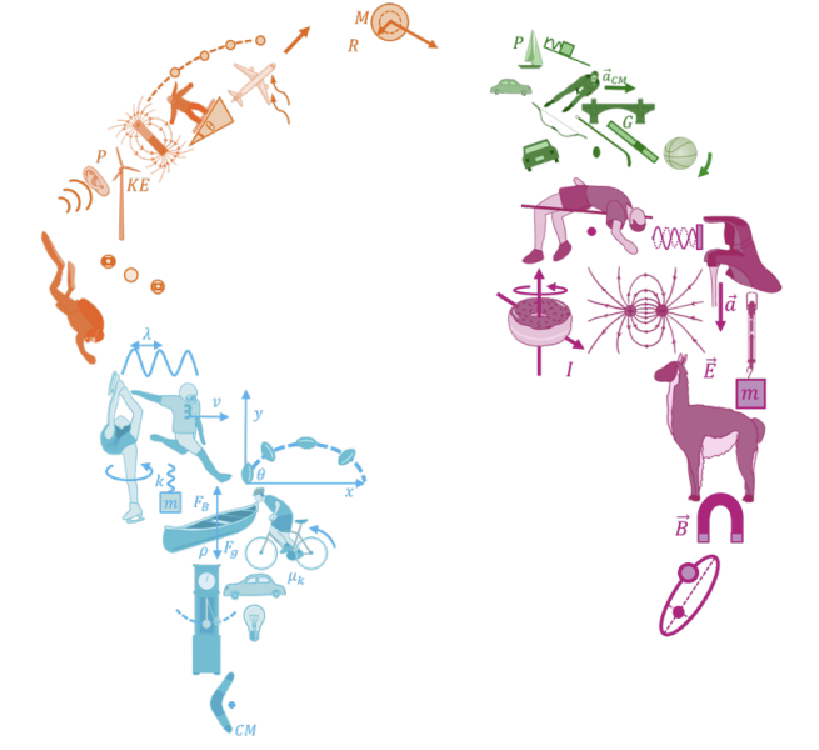
\includegraphics[width=4cm]{figures/BMDW/logo}
\end{textblock*}

\end{frame}




%%%%%%%%%%%%%TOC
\twocolframe{Outline}
  {\tableofcontents[sections={43,44}, subsectionstyle=show/show]\thispagestyle{empty}}
  {\tableofcontents[sections={45}, subsectionstyle=show/show]}
%%%%%%%%%%%%%%%%%%%%%%%%%


%%%%%%%%%%%%%%%%%%%%%%%%%%%%


\section{Induction}
\label{sec:induction}
\title{Induction}


%%%%%%%%%%%%%%%%%%%%%%%%%
\begin{frame}
\titlepage
\thispagestyle{empty}
\end{frame}






%%%%%%%%%%%%%%%%%%%%%%%%%%%%%%%%
\subsection{Charging a neautral electroscope}
\label{subsec:charginganeutralelectroscope}
\begin{frame}{Charging by induction}
\begin{center}
\begin{tikzpicture}[scale=1]
\tikzmath{
\h=3;
\L=3;
\dx=0.1;
\R=0.5;
\th=-60;
}
\scalebox{1}{

\only<1,4>{
\tikzmath{\th=-85;}
}

%electroscope
\draw (-\dx,-\R) rectangle (\dx,-\R-\h);
\draw (0,0) circle (\R);
\draw[line width = 4] (0,-\R-0.5*\h) -- +(\th:0.5*\h);


\only<2-4>{
%rod:
\draw[rounded corners] (45:1.75*\R) rectangle +(\L,4*\dx);
%charges on rod:
\foreach \i in {0, 0.1, ..., 1.1}{
\node[color=myred,above=-4pt] at ($(45:1.75*\R)+(\i*\L,4*\dx)$) {\scriptsize $-$};
\node[color=myred,below=-4pt] at ($(45:1.75*\R)+(\i*\L,0)$) {\scriptsize $-$};
}
\node[color=myred, left=-2pt] at ($(45:1.75*\R)+(0,2*\dx)$) {\scriptsize $-$};
\node[color=myred, right=-2pt] at ($(45:1.75*\R)+(\L,2*\dx)$) {\scriptsize $-$};
}


\only<2-4>{
%charges on electroscope
\foreach \i in {30,60,...,360}{
 \node[color=myblue!60] at (\i:1.1*\R) {\scriptsize $+$};
 }
 \only<2>{
\foreach \i in {0.2,0.4,...,1}{
  \node[color=myred, left] at ($(0,-\R-0.5*\h)+(0,-\i*0.5*\h) $) {\scriptsize $-$};
  \node[color=myred, above] at ($(0,-\R-0.5*\h)+(\th:\i*0.5*\h) $) {\scriptsize $-$};
 }
 }
}

\only<3>{
\draw[line width=1] plot[smooth] coordinates {(0,-\R-0.25*\h) (\h,-\R-0.45*\h) (\h,-\R-0.8*\h) (1.2*\h,-\R-\h)};
\foreach \i in {0.,0.2,...,0.8}{
  \node[color=myred, above] at ($(1.2*\h,-\R-\h)+(135:\i*0.25*\h) $) {\scriptsize $-$};
  \node[color=myred, left] at ($(1.2*\h,-\R-\h)+(135:\i*0.25*\h) $) {\scriptsize $-$};
 }

}

\only<5>{
%charges on electroscope
\foreach \i in {60,120,...,360}{
 \node[color=myblue!60] at (\i:1.1*\R) {\scriptsize $+$};
 }
\foreach \i in {0.2,0.4,...,1}{
  \node[color=myblue!60, left] at ($(0,-\R)+(0,-\i*\h) $) {\scriptsize $+$};
  \node[color=myblue!60, right] at ($(0,-\R)+(0,-\i*\h) $) {\scriptsize $+$};
 }
 \node[color=myblue!60, above=2pt] at ($(0,-\R-0.5*\h)+(\th:0.35*\h) $) {\scriptsize $+$};
 \node[color=myblue!60, below=] at ($(0,-\R-0.5*\h)+(\th:0.5*\h) $) {\scriptsize $+$};
}

}

\end{tikzpicture}
\captionof*{figure}{\textit{Charging an electroscope by induction.\only<1>{ Electroscope is neutral.}\only<2>{ Electroscope is neutral but charges separate.}\only<3>{ Charges opposite of those on the rod can escape through the ground wire.}\only<4>{ The ground wire is disconnected, positive charges stay on electroscope.}\only<5>{ Charges redistribute along the electroscope, leaving it charged.} }}
\end{center}
\end{frame}


%%%%%%%%%%%%%%%%%%%%%%%%%%%%%%%%




%%%%%%%%%%%%%%%%%%%%%%%%%%%%%%%%
\subsection{Dirod generator}
\label{subsec:dirodgenerator}
\begin{frame}{The dirod generator}
\begin{center}
\begin{tikzpicture}[scale=1]
\tikzmath{
\L=4;
\R=2.5;
\r=0.25;
\throds1=180;
\throds2=\throds1+180;
}

\scalebox{1}{

\only<1>{
\tikzmath{
  \throds1=180;
  \throds2=\throds1+180;
  }
}

\only<2>{
\tikzmath{
  \throds1=150;
  \throds2=\throds1+180;
  }
}


\only<3>{
\tikzmath{
  \throds1=120;
  \throds2=\throds1+180;
  }
}


\only<4>{
\tikzmath{
  \throds1=90;
  \throds2=\throds1+180;
  }
}


\only<5>{
\tikzmath{
  \throds1=60;
  \throds2=\throds1+180;
  }
}


\only<6->{
\tikzmath{
  \throds1=30;
  \throds2=\throds1+180;
  }
}



\draw[line width=1.5] (0,0) circle(\R);

\foreach \th in {30,60,...,360}{
  \ifthenelse{\th=\throds1 \OR \th=\throds2}{
     \fill[color=myblue!80] (\th:\R) circle (\r);
   }{
     \fill[color=myblue!40] (\th:\R) circle (\r);
  }
}

\draw[-latex] (-30:0.5*\R) arc (-30:-270:0.5*\R);

%plates:
\draw[line width=4, color=black] (1.5*\R,-\R) -- (1.5*\R,\R)node[above]{conducting plate};
\draw[line width=4, color=black] (-1.5*\R,-\R) -- (-1.5*\R,\R)node[above]{conducting plate};

%connectors
\draw[line width=2,color=myred] (0:\R-\r) -- (180:\R-\r)node[midway,above]{conductor};;
\draw[line width=2,color=myred] (-1.5*\R,-0.5*\R) -- +(0.55*\R,0) node[midway,below]{brush};
\draw[line width=2,color=myred] (1.5*\R,0.5*\R) -- +(-0.55*\R,0) node[midway,above]{brush};

%charges on plates
\only<1-7>{
\foreach \i in {0.1,0.2,...,0.9}{
  \node[left] at ($(-1.5*\R,-\R)+(0,\i*2*\R)$) {$-$};
  \node[right] at ($(1.5*\R,-\R)+(0,\i*2*\R)$) {$+$};
}
}

\only<8>{
\foreach \i in {0.05,0.1,...,0.95}{
  \node[left] at ($(-1.5*\R,-\R)+(0,\i*2*\R)$) {$-$};
  \node[right] at ($(1.5*\R,-\R)+(0,\i*2*\R)$) {$+$};
}
}

%charges on rods
\only<1-6>{
\foreach \th in {30,60,...,360}{
  \node at ($(\throds1:\R)+(\th:1.2*\r)$){+};
  \node at ($(\throds2:\R)+(\th:1.2*\r)+(0,-0.05)$){-};
 }
}

\only<7>{
%charges on brushes
\foreach \i in {0.2,0.4,...,0.8}{
  \node[above] at ($(-1.5*\R,-0.5*\R)+(\i*0.55*\R,0)$) {$-$};
  \node[below] at ($(1.5*\R,0.5*\R)+(-\i*0.55*\R,0)$) {$+$};
}

}

}

\end{tikzpicture}
\captionof*{figure}{\textit{A dirod generator works by inducing charges on the rotating cylinders and transferring those charges to plates.}}
\end{center}
\end{frame}


%%%%%%%%%%%%%%%%%%%%%%%%%%%%%%%%



\section{Coloumb's Law}
\label{sec:coulombslaw}
\title{Coloumb's Law}


%%%%%%%%%%%%%%%%%%%%%%%%%
\begin{frame}
\titlepage
\thispagestyle{empty}
\end{frame}



%%%%%%%%%%%%%%%%%%%%%%%%%%%%%%%%
\subsection{Coulomb's discovery}
\label{subsec:coulombdiscovery}
\twocolframesf{What did Coulomb observe?}
{
\begin{itemize}
\item<1-> Force is proportional to charges and the direction depends on their relative sign:
\begin{align*}
F\propto Q_1 Q_2
\end{align*}
\item<2-> Both charges feel equal and opposite force:
\begin{align*}
\vec F_{12}=-\vec F_{21}
\end{align*}
\item<3-> Inversely proportional to distance squared:
\begin{align*}
F&\propto \frac{1}{r^2}\\
\only<4>{
\therefore F&\propto \frac{Q_1Q_2}{r^2}=k\frac{Q_1Q_2}{r^2}}
\end{align*}
\end{itemize}
}
{
\vspace{-1.5cm}
\capfig{0.5}{figures/ChargesFields/Coulomb}{https://en.wikipedia.org/wiki/Charles-Augustin\_de\_Coulomb}
\vspace{-0.5cm}
\capfig{0.35}{figures/ChargesFields/CoulombExperiment}{Coulomb's experiment }
}


%%%%%%%%%%%%%%%%%%%%%%%%%%%%%%%%
\subsection{Recall: Newton's gravity}
\label{subsec:recallnewtonsgravity}
\twocolframesf{Recall Newton's Universal Theory of Gravity}
{
The force, $\vec F_{12}$, \textbf{on} mass $M_1$ \textbf{from} $M_2$ can be written as:
\begin{align*}
\vec F_{12} = - G \frac{M_1M_2}{r_{21}^2}\hat r_{21}=-G \frac{M_1M_2}{r_{21}^{\textcolor{myred}{3}}} \textcolor{myred}{\vec r_{21}}
\end{align*}
where:
\begin{itemize}
\item $\vec r_{21}=\vec r_2 - \vec r_1$ is the vector from $M_2$ to $M_1$.
\item $\hat r_{21}$ is the unit vector in the $\vec r_{21}$ direction.
\item $G=\SI{6.67e-11}{Nm^2/kg^2}$ is the Universal Gravitational Constant.
\item The force is always attractive due to the minus sign at the front.
\end{itemize}

}
{
\begin{center}
\begin{tikzpicture}
\tikzmath{
\L=4;
}
\scalebox{1}{

\coordinate (M1) at (0.2*\L, 0.6*\L);
\coordinate (M2) at (0.8*\L, 0.75*\L);

\draw[-latex,line width=1.5] (0,0) -- (\L,0) node[below]{$x$};
\draw[-latex,line width=1.5] (0,0) -- (0,\L) node[left]{$y$};

\fill (M1) circle (3pt) node[above left]{$M_1$};
\fill (M2) circle (3pt) node[above right]{$M_2$};

\draw[-latex,line width=1] (0,0) -- (M1) node[midway,right] {$\vec r_1$};
\draw[-latex,line width=1] (0,0) -- (M2) node[midway,right] {$\vec r_2$};

\draw[-latex,line width=2, color=myred] ($(M1)+(0,0.3)$) -- ($(M1)!0.4!(M2)+(0,0.3)$) node[above] {$\vec F_{12}$};
\draw[-latex,line width=1.5, color=myblue!60] (M2) -- (M1) node[midway,below] {$\vec r_{21}$};

}

\end{tikzpicture}
\captionof*{figure}{\textit{Vectors in Newton's Universal Theory of Gravity. The force on $M_1$ is in the opposite direction of $\vec r_{21}$.}}
\end{center}
}



%%%%%%%%%%%%%%%%%%%%%%%%%%%%%%%%
\subsection{Coulomb's Law}
\label{subsec:coulombslaw}
\twocolframesf{Coulomb's Law}
{
The force, $\vec F_{12}$, \textbf{on} charge $Q_1$ \textbf{from} charge $Q_2$ can be written as:
\begin{align*}
\vec F_{12} = k \frac{Q_1Q_2}{r_{21}^2}\hat r_{21}=k \frac{Q_1Q_2}{r_{21}^{\textcolor{myred}{3}}} \textcolor{myred}{\vec r_{21}}
\end{align*}
where:
\begin{itemize}
\item $\vec r_{21}=\vec r_2 - \vec r_1$ is the vector from $Q_2$ to $Q_1$.
\item $\hat r_{21}$ is the unit vector in the $\vec r_{21}$ direction.
\item $k=\SI{9.989e9}{Nm^2/C^2}$ is Coulomb's constant.
\item The force can be \textbf{attractive or repulsive}, depending on the product $Q_1Q_2$. If the charges are opposite, the product is negative and the force is attractive.
\end{itemize}

}
{
\begin{center}
\begin{tikzpicture}
\tikzmath{
\L=4;
}
\scalebox{1}{

\coordinate (M1) at (0.2*\L, 0.6*\L);
\coordinate (M2) at (0.8*\L, 0.75*\L);

\draw[-latex,line width=1.5] (0,0) -- (\L,0) node[below]{$x$};
\draw[-latex,line width=1.5] (0,0) -- (0,\L) node[left]{$y$};

\fill (M1) circle (3pt) node[above left]{$Q_1$} node[left,color=myred]{$-$};
\fill (M2) circle (3pt) node[above right]{$Q_2$}node[right,color=myred]{$+$};

\draw[-latex,line width=1] (0,0) -- (M1) node[midway,right] {$\vec r_1$};
\draw[-latex,line width=1] (0,0) -- (M2) node[midway,right] {$\vec r_2$};

\draw[-latex,line width=2, color=myred] ($(M1)+(0,0.3)$) -- ($(M1)!0.4!(M2)+(0,0.3)$) node[above] {$\vec F_{12}$};
\draw[-latex,line width=1.5, color=myblue!60] (M2) -- (M1) node[midway,below] {$\vec r_{21}$};

}

\end{tikzpicture}
\captionof*{figure}{\textit{Vectors in Coulomb's Law. The force is attractive if the charges have opposite signs.}}
\end{center}
}


%%%%%%%%%%%%%%%%%%%%%%%%%%%%%%%%
\subsection{Gravity and the electric force}
\label{subsec:gravityandtheelectricforce}
\begin{frame}{Gravity and the Electric force}
\begin{itemize}
\item Mathematically, these are almost identical; instead of mass, we have electric charge (can think of gravitational mass as gravitational charge).
\item The main difference is that electric charges can be positive or negative, which can make the force attractive or repulsive.
\item Since we can define a gravitational field, $\vec g$ , we should be able to define an ``electric'' field, $\vec E$:
\begin{align*}
\vec F_g = m\vec g \quad\quad \vec F_E=q\vec E
\end{align*}
\item Since Gauss' Law can allow us to determine the gravitational field, it should also work for the electric field (next week's topic!).

\end{itemize}
\end{frame}


%%%%%%%%%%%%%%%%%%%%%%%%%%%%%%%%
\subsection{Inverse square laws and waves}
\label{subsec:inversesquarelawsandwaves}
\begin{frame}{Inverse square laws and waves}
Recall: to conserve energy, the intensity of a wave must decrease with the square of distance.
\begin{itemize}
\item So, maybe, the ``forces at a distance'' (gravity and Coulomb) are somehow transmitted by a wave?
\item Coulomb Force is actually transmitted by light waves!
\item Gravity is transmitted by waves (Nobel Prize 2017)!
\end{itemize}
\end{frame}


%%%%%%%%%%%%%%%%%%%%%%%%%%%%%%%%




%%%%%%%%%%%%%

\section{The Electric Field}
\label{sec:thelectricfield}
\title{The Electric Field}


%%%%%%%%%%%%%%%%%%%%%%%%%
\begin{frame}
\titlepage
\thispagestyle{empty}
\end{frame}


%%%%%%%%%%%%



%%%%%%%%%%%%%%%%%%%%%%%%%%%%%%%%
\subsection{Derivation}
\label{subsec:derivation}
\begin{frame}{The electric field}
\begin{itemize}
\item Consider the electric force from 2 stationary charges:
\begin{align*}
\vec F = \vec F_1 + \vec F_2=k\frac{qQ_1}{r_1^2}\hat r_1+k\frac{qQ_2}{r_2^2}\hat r_2
\end{align*}
\item Since $q$ is a scalar, it can be factored out:
\begin{align*}
\vec F =q\left( k\frac{Q_1}{r_1^2}\hat r_1+k\frac{Q_2}{r_2^2}\hat r_2\right)
\end{align*}
\item We can easily get the force vector for $q\to -2q$ by just multiplying the part in parenthesis by $-2q$ instead of $q$.
\item The part in parenthesis is Force per Charge, or Electric field:
\begin{align*}
\vec E = \frac{\vec F}{q}
\end{align*}
\end{itemize}

\end{frame}


%%%%%%%%%%%%%%%%%%%%%%%%%%%%%%%%
\begin{frame}{Recall, gravitational field outside a spherical mass}
\begin{itemize}
\item At some distance $r$ from a (spherical) object of mass $M$, a mass $m$ feels a force:
\begin{align*}
\vec F = -G\frac{mM}{r^2}\hat r
\end{align*}
\item Force per unit mass (gravitational field) outside of a spherical body:
\begin{align*}
\vec g = \frac{F}{m}=-G\frac{M}{r^2}
\end{align*}
\item At the surface of the Earth (of radius, $R$):
\begin{align*}
\vec g = \frac{F}{m}=-G\frac{M}{R^2}
\end{align*}
\end{itemize}

\end{frame}


%%%%%%%%%%%%%%%%%%%%%%%%%%%%%%%%
\begin{frame}{Electric field}
\begin{itemize}
\item If you have a point charge, $Q$ at the origin, you can calculate the electric field vector at any point in space, at a position $\vec r$ :
\begin{align*}
\vec E = k\frac{Q}{r^2}\hat r
\end{align*}
\item To find the force vector on some other charge, $q$, you just multiply the value of the electric field by $q$:
\begin{align*}
\vec F_q=q\vec E
\end{align*}
\item The electric field is a ``Vector Field'' (it is a function that you can evaluate anywhere in space to obtain a vector).
\end{itemize}
\end{frame}


%%%%%%%%%%%%%%%%%%%%%%%%%%%%%%%%
\subsection{Field lines}
\label{subsec:fieldlines}
\twocolframesf{Visualizing the electric field: Field Lines}
{
\begin{itemize}
\item We can draw ``field lines'' that tell us how to determine the electric field vector at some point in space:
\begin{itemize}
\item The more lines there are in an area of space, the stronger the electric field (the longer the vector) and corresponding force.
\item The electric field vector is always tangent to the field lines.
\item The electric field vector is always \textbf{in the direction of the force that a positive charge would feel}.
\end{itemize}
\end{itemize}
}
{
\vspace{-1.5cm}
\begin{center}
\begin{tikzpicture}
\tikzmath{
\L=2.5;
}
\scalebox{1}{

\begin{scope}
\clip (-0.6*\L,-0.6*\L) rectangle (0.6*\L,0.6*\L);
\foreach \th in {0,10,...,360}{
\draw (0,0) -- (\th:\L);
\draw[latex-] (\th:0.4*\L) -- +(\th:-0.2);
}
\end{scope}
\fill[color=myred] (0,0) circle (3pt);
\node[color=white] at (0,0){+};

\draw[latex-,line width=1.5,color=myred] (40:0.75*\L) -- +(40:-0.15*\L);
\draw[latex-,line width=1.5,color=myred] (-40:0.4*\L) -- +(-40:-0.25*\L);

}
\end{tikzpicture}
\captionof*{figure}{\textit{Electric field lines out of a positive point charge.}}
\end{center}


\begin{center}
\begin{tikzpicture}
\tikzmath{
\xe=-2;%Coordinates of first mass/charge (Earth)
\ye=0;
\xm=2;%Coordinates of first mass/charge (Moon)
\ym=0;
\mee=1;% Mass/charge of first mass (Earth)
\mmm=0.6;% Mass/charge of first mass (Earth)
\dl=0.1;%scale factor to advance along the field line
\n=35;%number of points to find in the line (make as small as possible to reach the point you want!)
}

\scalebox{1}{
%Top field lines (xst is the starting x position of the field line)
\foreach \xst in {-2.8,-2.4,...,2.4}{
  \tikzmath{
  \yst=1.5; %all field lines start at yst
  \x=\xst;
  \y=\yst;
  %
  %generate points on the line (keeps finding the next point)
  int \i;
  %note that this also creates \mypairx and \mypairy!
  coordinate \mypair;
  for \i in {1,...,\n}{
    %First mass (earth)
    \re=(\x-\xe)*(\x-\xe)+(\y-\ye)*(\y-\ye)+0.0001;
    \Fex=\mee*(\x-\xe)/\re;
    \Fey=\mee*(\y-\ye)/\re;
    %Second mass (moon)
    \rm=(\x-\xm)*(\x-\xm)+(\y-\ym)*(\y-\ym)+0.0001;
    \Fmx=\mmm*(\x-\xm)/\rm;
    \Fmy=\mmm*(\y-\ym)/\rm;
    %Total force:
    \Fx=\Fex+\Fmx;
    \Fy=\Fey+\Fmy;
    \Fn=sqrt(\Fx*\Fx+\Fy*\Fy)+0.0001;
    \dx=\Fx/\Fn*\dl;
    \dy=\Fy/\Fn*\dl;
    \x=\x-\dx;
    \y=\y-\dy;
    \mypair{\i}=(\x,\y);
    };
  }
  %Draw that field line
  \foreach \i in {2,...,\n}{
    \tikzmath{
    int \im;
    \im=\i-1;
    }
    \draw (\mypair{\im}) -- (\mypair{\i});
    \ifthenelse{\im =5}{\draw[latex-] (\mypair{\im}) -- (\mypair{\i})}{};%draw arrow on the fifth point
  }

}%end of loop over x

%Bottom field lines
\foreach \xst in {-2.8,-2.4,...,2.4}{
  \tikzmath{
  \yst=-1.5;
  \x=\xst;
  \y=\yst;
  %
  %generate points on the line
  int \i;
  %note that this also creates \mypairx and \mypairy!
  coordinate \mypair;
  for \i in {1,...,\n}{
    %First mass (earth)
    \re=(\x-\xe)*(\x-\xe)+(\y-\ye)*(\y-\ye)+0.0001;
    \Fex=\mee*(\x-\xe)/\re;
    \Fey=\mee*(\y-\ye)/\re;
    %Second mass (moon)
    \rm=(\x-\xm)*(\x-\xm)+(\y-\ym)*(\y-\ym)+0.0001;
    \Fmx=\mmm*(\x-\xm)/\rm;
    \Fmy=\mmm*(\y-\ym)/\rm;
    %Total force:
    \Fx=\Fex+\Fmx;
    \Fy=\Fey+\Fmy;
    \Fn=sqrt(\Fx*\Fx+\Fy*\Fy)+0.0001;
    \dx=\Fx/\Fn*\dl;
    \dy=\Fy/\Fn*\dl;
    \x=\x-\dx;
    \y=\y-\dy;
    \mypair{\i}=(\x,\y);
    };
  }
  %Draw that field line
  \foreach \i in {2,...,\n}{
    \tikzmath{
    int \im;
    \im=\i-1;
    }
    \draw (\mypair{\im}) -- (\mypair{\i});
    \ifthenelse{\im =5}{\draw[latex-] (\mypair{\im}) -- (\mypair{\i})}{};
  }

}%end of loop over x

%Draw the charges
\fill[color=myred] ((\xe,\ye)  circle (6pt);
\node[color=white] at (\xe,\ye) {$+$};

\fill[color=myred] (\xm,\ym) circle (3pt);
\node[color=white] at (\xm,\ym){$+$};


}

\end{tikzpicture}
\captionof*{figure}{\textit{Electric field lines from two different positive charges.}}
\end{center}


}

%%%%%%%%%%%%%%%%%%%%%%%%%%%%%%%%



















%%%%%%%%%%%%%%%%%%%%%%%%%%%%%%%%


%%%%%%%%%%%%%%%%%%%%%%%%%%%%%%%%
\subsection{Superposition}
\label{subsec"superposition}
\twocolframesf{Electric field and superposition}
{
\begin{itemize}
\item If there are multiple charges, one can add the electric field from each charge to get the total electric field at one point in space.
\item If we have continuous charge distributions (as opposed to point charges), then we can model those distributions as being the sum of many individual point charges.
\item The total electric field can be found by adding the infinitesimal electric fields from each (point) charge element:
\begin{align*}
d\vec E &= k\frac{dq}{r^2}\hat r\\
\vec E &= \int d\vec E
\end{align*}
\end{itemize}
}
{
\begin{center}
\begin{tikzpicture}

\scalebox{1}{

\draw[line width=1.5] (0,0) ..controls (2,1) and (0,4).. (2,4);


\fill[myblue!60] (1,1.6) circle(3pt);
\fill[myblue!60] (1,1.8) circle(3pt);
\fill[myred] (1,2) circle(3pt) node[left]{$dq$};
\fill[myblue!60] (1,2.2) circle(3pt);
\fill[myblue!60] (1,2.4) circle(3pt);

\fill (2,2) circle (2pt) node[below]{$P$};
\draw[-latex] (1,2) -- (2,2) node[midway,below]{$\vec r$};
\draw[-latex, line width=2] (2,2) -- +(1,0) node[midway,above]{$d\vec E$};
}
\end{tikzpicture}
\captionof*{figure}{\textit{To determine the electric field at point $P$ from a charge distribution, model the distribution as a collection of point charges, $dq$, and add those fields together.}}
\end{center}
}


%%%%%%%%%%%%%%%%%%%%%%%%%%%%%%%%



%%%%%%%%%%%%%%%%%%%%%%%%%%%%%%%%
\subsection{Electric field from a half-ring of charge}
\label{subsec:electricfieldfromahalfringofcharge}
\twocolframesf{Electric field from a half-ring of charge}
{
\only<1-6>{
\begin{enumerate}
\item Make a \textit{good} diagram.
\item<2-> Choose a charge element, \textcolor{myred}{$dq$}.
\item<3-> Draw the electric field element, \textcolor{myred}{$d\vec E$}, due to $dq$.
\item<4-> Write the electric field element, \textcolor{myred}{$d\vec E$}, using relevant variables:
\begin{align*}
d\vec E = \frac{k dq}{R^2}(\cos\theta \hat x -\sin\theta \hat y) = dE_x\hat x + dE_y \hat y
\end{align*}
\item<5-> Think of symmetry! ($\int dE_y=0$)
\item<6-> Write the electric field as the sum of the $d\vec E$:
\begin{align*}
\vec E = \int d\vec E = \left(\int dE_x\right)\hat x + \cancelto{0}{\left(\int dE_y\right)}\hat y
\end{align*}
\end{enumerate}
}
\only<7->{
\begin{enumerate}
\setcounter{enumi}{6}
\item We will choose, $\theta$, as the the integration variable:
\begin{align*}
E_x = \int dE_x =  \int_{\frac{-\pi}{2}}^{\frac{\pi}{2}} \frac{k dq}{R^2}\cos\theta
\end{align*}
\item Introduce charge per unit length, $\lambda=\frac{Q}{\pi R}$:
\begin{align*}
dq &= \lambda R d\theta=\frac{Q}{\pi R} Rd\theta=\frac{Q}{\pi}d\theta\\
\therefore E_x &= \int_{\frac{-\pi}{2}}^{\frac{\pi}{2}} \frac{k Q }{\pi R^2}\cos\theta d\theta\\
&=\frac{k Q }{\pi R^2} \int_{\frac{-\pi}{2}}^{\frac{\pi}{2}} \cos\theta d\theta = \frac{k Q }{\pi R^2}\left[\sin\theta\right]_{\frac{-\pi}{2}}^{\frac{\pi}{2}} =  \frac{2k Q }{\pi R^2}
\end{align*}
\end{enumerate}
}
}
{
\begin{center}
\begin{tikzpicture}
\tikzmath{
\R=2;
}
\scalebox{1}{

\draw[line width=3] (0,\R) arc(90:270:\R);
\draw[-latex] (0,0) -- +(1,0) node[below]{$x$};
\draw[-latex] (0,0) -- +(0,1) node[left]{$y$};
\node[above] at (110:\R) {$Q$};

\only<2->{
\draw[line width=3, color=myred] (130:\R) arc (130:140:\R) node[midway,above]{$dq$};
\draw[dashed, line width =1.5, color=myred] (0,0) -- (180:\R);
\draw[dashed, line width =1.5, color=myred] (0,0) -- (135:\R) node[midway,above]{$R$};
\draw[color=myred] (180:0.7) arc(180:135:0.7) node[midway,left]{$\theta$};
}

\only<3->{
\draw[-latex, line width=2, color=myred] (0,0) -- (-45:0.5*\R) node[below]{$d\vec E$};
}

\only<5>{
\draw[line width=3, color=myblue!60] (220:\R) arc (220:230:\R) node[midway,below]{$dq'$};
\draw[-latex, line width=2, color=myblue!60, dashed] (0,0) -- (45:0.5*\R) node[above]{$d \pvec E'$};
\draw[dashed, line width =1.5, color=myblue!60] (0,0) -- (225:\R);
}


}
\end{tikzpicture}
\captionof*{figure}{\textit{Modeling the electric field from a half-ring of charge, $Q$.}}
\end{center}
}



%%%%%%%%%%%%%%%%%%%%%%%%%%%%%%%%
\subsection{Electric field from an infinite line charge}
\label{subsec:electricfieldfromaninfinitelinecharge}
\twocolframesf{Electric field from an infinite line charge}
{
\only<1-5>{
\begin{enumerate}
\item Make a \textit{good} diagram.
\item<2-> Choose a charge element, \textcolor{myred}{$dq$}.
\item<3-> Draw the electric field element, \textcolor{myred}{$d\vec E$}, due to $dq$.
\item<4-> Write the electric field element, \textcolor{myred}{$d\vec E$}, using relevant variables:
\begin{align*}
d\vec E = \frac{k dq}{r^2}(\cos\theta \hat x -\sin\theta \hat y) = dE_x\hat x + dE_y \hat y
\end{align*}
\item<5-> Think of symmetry! ($\int dE_y=0$):
\begin{align*}
\vec E = \left(\int \frac{k dq}{r^2}\cos\theta\right) \hat x
\end{align*}
%\item<6-> Write the electric field as the sum of the $d\vec E$:
%\begin{align*}
%\vec E = \int d\vec E = \left(\int dE_x\right)\hat x + \cancelto{0}{\left(\int dE_y\right)}\hat y
%\end{align*}
\end{enumerate}
}
\only<6-7>{
\vspace{-0.75cm}
\begin{align*}
\vec E = \left(\int \frac{k dq}{r^2}\cos\theta\right) \hat x
\end{align*}
\vspace{-0.5cm}
\begin{enumerate}
\setcounter{enumi}{5}
\item<6-> We can integrate over $\theta$ or $y$, we choose $y$. Anything that changes with different $dq$ needs to be expressed with $y$ and constants:
\begin{align*}
dq = \lambda dy\;\;\text{and}\;\;  r^2=R^2+y^2 \;\;\text{and}\;\; \cos\theta=\frac{R}{\sqrt{R^2+y^2}}
\end{align*}
\item<7-> All together:
\begin{align*}
E_x = \int_{-\infty}^{+\infty} \frac{k \lambda dy R}{\left(y^2+R^2  \right)^{\frac{3}{2}}}=k\lambda R\int_{-\infty}^{+\infty} \frac{ dy}{\left(y^2+R^2  \right)^{\frac{3}{2}}}
\end{align*}
ask your math friend for help, look it up...
\end{enumerate}
}
\only<8->{
\vspace{-0.75cm}
\begin{align*}
\vec E = \left(\int \frac{k dq}{r^2}\cos\theta\right) \hat x
\end{align*}
\vspace{-0.5cm}
\begin{itemize}
\item<8-> What if we integrate over $\theta$?
\only<9->{
\vspace{-0.5cm}
\begin{align*}
y=R\tan\theta \;\;\rightarrow\;\;\frac{dy}{d\theta}=\frac{R}{\cos^2\theta}\\
\therefore dq = \lambda dy=\lambda\frac{R}{\cos^2\theta} d\theta \;\;\text{and}\;\;  r^2=\frac{R^2}{\cos^2\theta}
\end{align*}}
\item<10-> All together:
\begin{align*}
E_x &= \int_{-\frac{\pi}{2}}^{+\frac{\pi}{2}} k\lambda\frac{Rd\theta}{\cos^2\theta}\frac{\cos^2\theta}{R^2}\cos\theta=\frac{k\lambda}{ R}\int_{-\frac{\pi}{2}}^{+\frac{\pi}{2}} \cos\theta d\theta\\
 &= \frac{2k\lambda}{ R}
\end{align*}
\end{itemize}
}
}
{
\begin{center}
\begin{tikzpicture}
\tikzmath{
\L=5;
\R=2;
\thq=30;
\hq=\R*tan(\thq);
\dx=0.4;
}
\scalebox{1}{

\draw[line width=3] (-\R,-\L/2) -- (-\R,\L/2);
\draw[-latex] (0,0) -- +(1,0) node[below]{$x$};
\draw[-latex] (0,0) -- +(0,1) node[left]{$y$};
\fill (0,0) circle (2pt);
\draw[latex-latex, line width=1.5] (0,0) -- (-\R, 0) node[midway,below]{$R$};
\node[right] at (-\R,\L/2) {$\lambda$};

\only<2->{
\draw[line width=3, color=myred] (-\R,\hq-0.5*\dx) -- +(0,\dx) node[midway,left]{$dq$};
\node[right, color=myred] at (-\R,0.5*\hq){$y$};
\draw[dashed, line width =1.5, color=myred] (0,0) -- (-\R,\hq) node[midway,above]{$r$};
\draw[color=myred] (180:0.7) arc(180:180-\thq:0.7) node[midway,left]{$\theta$};
}

\only<3->{
\draw[-latex, line width=2, color=myred] (0,0) -- (-\thq:1) node[below]{$d\vec E$};
}

\only<5>{
\draw[line width=3, color=myblue!60] (-\R,-\hq-0.5*\dx) -- +(0,-\dx) node[midway,left]{$dq'$};
\draw[-latex, line width=2, color=myblue!60, dashed] (0,0) -- (\thq:1) node[above]{$d \pvec E'$};
\draw[dashed, line width =1.5, color=myblue!60] (0,0) -- (-\R,-\hq) ;
}


}
\end{tikzpicture}
\captionof*{figure}{\textit{Modeling the electric field at a distance, $R$, from an infinite line of charge.}}
\end{center}
}


%%%%%%%%%%%%%%%%%%%%%%%%%%%%%%%%


%%%%%%%%%%%%%%%%%%%%%%%%%%%%%%%%
\subsection{2D infinite plane}
\label{subsec:2dinfiniteplane}
\twocolframesf{2D infinite plane}
{
\begin{itemize}
\item If you have a continuous 2D (3D) charge distribution, model it as the sum of electric fields from 1D (2D) charge distributions.
\item For example, for an infinite plane (2D), consider it has being made of many infinite lines of charge (1D), for which you just calculated the electric field.
\begin{itemize}
\item The plane has surface charge density, $\sigma$.
\item An infinite line of charge with width dy thus has linear charge density:
\begin{align*}
\lambda = \sigma dy
\end{align*}
\item Sum all of the electric fields from lines of charge at different values of $y$.
\end{itemize}

\end{itemize}
}
{
\vspace{-1cm}
\begin{center}
\begin{tikzpicture}
\tikzmath{
\L=4;
\thyz=30;%perspective angle
\Ly=4;
\dy=0.3;
}
\scalebox{1}{
\coordinate (P1) at ($(180+\thyz:\Ly/2)-(0,0.5*\L)$);
\coordinate (P2) at ($(P1)+(0,\L)$);
\coordinate (P3) at ($(P2)+(\thyz:\Ly)$);
\coordinate (P4) at ($(P3)+(0,-\L)$);
%strip
\coordinate (P5) at ($(\thyz:0.35*\Ly)-(0,0.5*\L)$);
\coordinate (P6) at ($(P5)+(0,\L)$);
\coordinate (P7) at ($(P6)+(\thyz:\dy)$);
\coordinate (P8) at ($(P7)+(0,-\L)$);

\fill[color=myblue!40] (P1) -- (P2) -- (P3) -- (P4) -- cycle;
\fill[color=myblue!80] (P5) -- (P6) -- (P7) -- (P8) -- cycle;
\draw[line width=1,-latex] (0,0) -- +(\thyz:\Ly) node[above]{$y$};
\draw[line width=1,-latex] (0,0) -- +(\Ly,0) node[above]{$z$};
\draw[line width=1,-latex] (0,0) -- +(0,-0.75*\L) node[right]{$x$};

\coordinate (PY) at (\thyz:0.35*\Ly+0.5*\dy);
\coordinate (PZ) at (0.7*\Ly,0);
\coordinate (PE) at ($(PY)!1.5!(PZ)$);

\node[above] at (\thyz:\Ly/8) {$y$};
\fill (PZ) circle (3pt) node[above=2pt]{$P$};
\draw[line width = 1, dashed ] (PY) -- ($(PY)!2!(PZ)$);
\node[above] at ($(PY)!0.5!(PZ)$) {$r$};
\draw[line width = 2, color=myred, -latex] (PZ) -- (PE) node[below]{$d\vec E$};
\draw[color=myred] ($(PZ)+(0.7,0)$) arc(0:-30:0.7)node[midway,right]{$\theta$};
\draw[latex-latex,color=myred] ($(P6)+(0,0.2)$) -- ($(P7)+(0,0.2)$) node[midway,above]{$dy$};
}
\end{tikzpicture}
\captionof*{figure}{\textit{The electric field from an infinite plane with charge per unit area, $\sigma$. By symmetry, the net field will be in the $y$ direction.}}
\end{center}
}


%%%%%%%%%%%%%%%%%%%%%%%%%%%%%%%%
\subsection{2D infinite plane, method 2}
\label{subsec:2dinfiniteplanemethod2}
\twocolframesf{{2D infinite plane, different method}}
{
\begin{itemize}
\item You can model the infinite plane as the sum of rings. 
\item A ring of width $dr$ has  total charge given by:
\begin{align*}
dq=\sigma 2 \pi r dr
\end{align*}
\item Sum all of the electric fields from all of the rings, from $r=0$ to $r=\infty$.
\end{itemize}
}
{
\begin{center}
\begin{tikzpicture}
\tikzmath{
\L=4;
\thyz=45;%perspective angle
\Ly=3.5;
\R=2.5;
\r=0.75*\R;
\dr=0.3;
}
\scalebox{1}{

\fill[color=myblue!40] (0,0) circle({\R} and {\R/4});
\fill[color=myblue!80] (0,0) circle({\r} and {\r/4});
\fill[color=myblue!40] (0,0) circle({\r-\dr} and {(\r-\dr)/4});

\draw[line width=1,-latex] (0,0) -- +(270-\thyz:0.75*\Ly) node[left]{$x$};
\draw[line width=1,-latex] (0,0) -- +(\Ly,0) node[above]{$y$};
\draw[line width=1,-latex] (0,0) -- +(0,0.75*\Ly) node[right]{$z$};

\draw[latex-latex,color=myred] (0,-0.1) -- +(\r-\dr,0) node[midway,below]{$r$};
\draw[latex-latex,color=myred] (-\r,0) -- +(\dr,0) node[midway,above]{$dr$};
\draw[-latex,color=myred, line width=1.5] (0,0.3*\Ly) -- +(0,0.75) node[right]{$d\vec E$};
\fill (0,0.3*\Ly) circle(2pt) node[left]{$P$};
}
\end{tikzpicture}
\captionof*{figure}{\textit{The electric field from an infinite plane with charge per unit area, $\sigma$. By symmetry, the net field will be in the $y$ direction.}}
\end{center}
}

%%%%%%%%%%%%%%%%%%%%%%%%%%%%%%%%



\subsection{Electric dipoles}
\label{subsec:electricdiapoles}
\twocolframesf{Electric dipoles}
{
\begin{itemize}
\item Dipoles are a pair of equal magnitude but opposite sign charges, $Q$, separated by a fixed distance, $l$.
\item For example, a water molecule can be modeled as a dipole.
\end{itemize}
}
{
\begin{center}
\begin{tikzpicture}
\tikzmath{
\L=3;
\R=0.75;
}
\scalebox{1}{
\draw[line width=3, color=myblue!60](0,0) -- (20:\L) node[midway,above]{$l$};
\fill[color=myblue!60] (0,0) circle (7pt) node[color=white]{$-$} node[above=5pt,color=black]{$-Q$};
\fill[color=myblue!60] (20:\L) circle (7pt) node[color=white]{$+$} node[above=5pt,color=black]{$+Q$};

\begin{scope}[shift={(0.5*\L,-0.5*\L)}]

\shade[ball color=myred] (30:1.1*\R) circle(0.5*\R);
\shade[ball color=myred] (150:1.1*\R) circle(0.5*\R);
\shade[ball color=myblue!60] (0,0) circle(\R);
\node[below] at (0,-\R){$--$};
\node at (30:1.8*\R){$+$};
\node at (150:1.8*\R){$+$};
\end{scope}

}
\end{tikzpicture}
\captionof*{figure}{\textit{A dipole and a water molecule.}}
\end{center}
}


%%%%%%%%%%%%%%%%%%%%%%%%%%%%%%%


%%%%%%%%%%%%%%%%%%%%%%%%%%%%%%%%
\twocolframesf{The dipole moment vector, $\vec p$}
{
\begin{itemize}
  \item We introduce the \textbf{dipole vector}, $\vec p$:
  \begin{itemize}
    \item Magnitude: $p=Ql$
    \item Direction from $-Q$ to $+Q$
  \end{itemize} 
  \item The net torque on the dipole is then given by:
  \begin{align*}
  \vec \tau &=\vec p \times \vec E\\
  \tau &= pE\sin\theta
  \end{align*}
\end{itemize} 
Check:
\begin{align*}
F_{\perp}&=QE\sin\theta\\
\therefore \tau &=F_\perp\frac{l}{2}+ F_\perp\frac{l}{2}\\
&= QEl\sin\theta=pE\sin\theta
\end{align*}
}
{
%\capfig{0.4}{figures/dipolefield}{A dipole in a field.}
\begin{center}
\begin{tikzpicture}
\tikzmath{
\L=3;
\R=0.75;
\th=45;
}
\scalebox{1}{

\foreach \h in {-0.6,-0.3,...,2.7}{
  \draw[color=black!30, line width=1,-latex] (-0.5,\h) -- (2.6,\h);
}
%\node[below] at (2.6,-0.6){$\vec E$};

\draw[line width=3, color=myblue!60](0,0) -- (\th:\L) node[midway,above]{$l$};
\fill[color=myblue!60] (0,0) circle (7pt) node[color=white]{$-$} node[below=5pt,color=black]{$-Q$};
\fill[color=myblue!60] (\th:\L) circle (7pt) node[color=white]{$+$} node[above=5pt,color=black]{$+Q$};
\draw[-latex,line width=2,color=myblue!60] ($ (0.75,0.3) $) -- +(\th:0.5*\L) node[below]{$\vec p$};
\draw[-latex,line width=2] ($ (0.75,0.3) $) -- (2.6,0.3) node[right]{$\vec E$};
\draw[color=myred]($ (0.75,0.3) +(0.7,0)$) arc(0:\th:0.7) node[midway,right]{$\theta$};

\draw[-latex,color=myred, line width=1.5] (0,0) -- (180:1.5) node[below]{$-\vec F$};
\draw[-latex,dotted,color=myred, line width=1.5] (0,0) -- (135:1) node[left]{$\vec F_\perp$};

\draw[-latex,color=myred, line width=1.5] (\th:\L) -- +(0:1.5) node[below]{$\vec F$};
\draw[-latex,dotted,color=myred, line width=1.5] (\th:\L) -- +(-45:1) node[right]{$\vec F_\perp$};
}
\end{tikzpicture}
\captionof*{figure}{\textit{A dipole, formed by two charges of magnitude, $Q$, a distance, $l$, apart in an electric field, $\vec E$.}}
\end{center}
}


%%%%%%%%%%%%%%%%%%%%%%%%%%%%%%%%




%%%%%%%%%%%%%%%%%%%%%%%%%%%%%%%%
\twocolframe{Dipole potential energy}
{
\begin{itemize}
  \item The potential energy is minimum when the dipole vector is parallel to the electric field.
  \item The potential energy is maximum when the dipole vector is anti-parallel to the electric field.
  \item We can write the potential energy:
  \begin{align*}
  U=-\vec p \cdot \vec E = -pE\cos\theta
  \end{align*}
\end{itemize} 
}
{
\begin{center}
\begin{tikzpicture}
\tikzmath{
\th=30;
}
\scalebox{1}{

\draw[-latex,line width=2,color=myblue!60] (0,0) -- +(1.5,0) node[midway,above]{$\vec p$};
\draw[-latex,line width=2] (0,-0.3) -- +(1.5,0) node[midway,below]{$\vec E$};
\node[right] at (1.75,-0.15) {$U=-pE$};

\begin{scope}[shift={(0,-2)}]
\draw[-latex,line width=2,color=myblue!60] (0,0) -- +(1.5,0) node[midway,above]{$\vec p$};
\draw[latex-,line width=2] (0,-0.3) -- +(1.5,0) node[midway,below]{$\vec E$};
\node[right] at (1.75,-0.15) {$U=pE$};
\end{scope}

\begin{scope}[shift={(0,-4)}]
\draw[-latex,line width=2,color=myblue!60] (0,0) -- +(\th:1.5) node[midway,above]{$\vec p$};
\draw[-latex,line width=2] (0,0) -- +(1.5,0) node[midway,below]{$\vec E$};
\draw (0.7,0) arc(0:\th:0.7) node[midway,right]{$\theta$};
\node[right] at (1.75,-0.15) {$U=-pE\cos\theta$};
\end{scope}

}
\end{tikzpicture}
\captionof*{figure}{\textit{A dipole in an electric field.}}
\end{center}
}

%%%%%%%%%%%%%%%%%%%%%%%%%%%%%%%%







































%%%%%%%%%%%%%%%%%%%%%%%%%%%%%%%%


\title{Gauss}
\subject{Gauss's Law, Flux and Application}
\subtitle{Building Models to Describe our World}


%%%%%%%%%%%%%%%%%%%%%%%%%%%%%%
%%%%%%%%%%%%%%%%%%%%%



%%%%%%%%%%%%%%%%%%%%%%%%%
%%%%%% Title slide %%%%%%
%%%%%%%%%%%%%%%%%%%%%%%%%
\chaptertitle{Gauss}
\begin{frame}
\label{chap:gauss}
\titlepage
\thispagestyle{empty}

\begin{textblock*}{5cm}(11cm,4cm)
    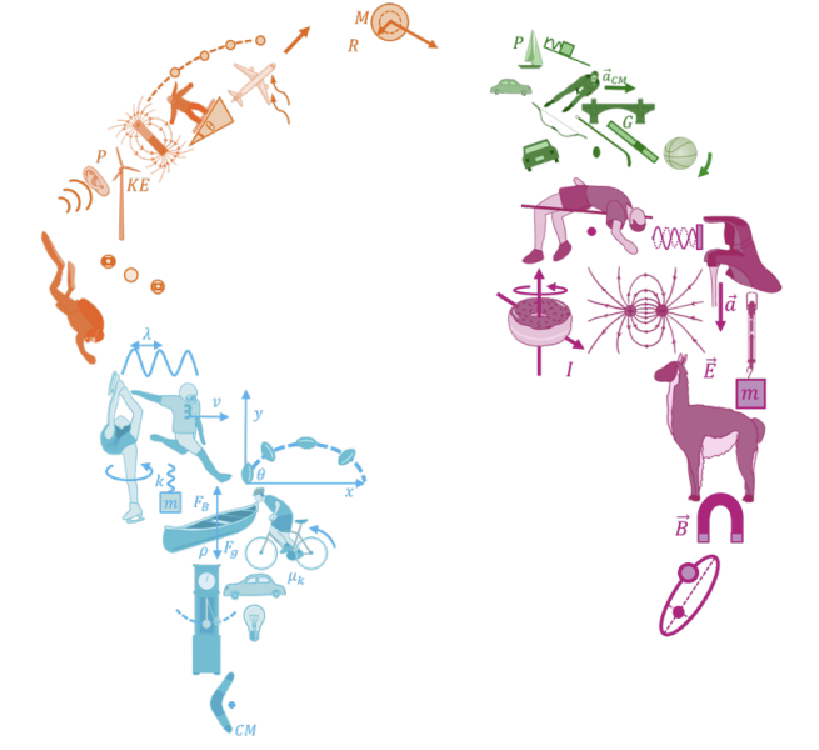
\includegraphics[width=4cm]{figures/BMDW/logo}
\end{textblock*}

\end{frame}

%%%%%%%%%%%%%TOC
\twocolframe{Outline}
  {\tableofcontents[sections={46}, subsectionstyle=show/show]\thispagestyle{empty}}
  {\tableofcontents[sections={47,48}, subsectionstyle=show/show]}
%%%%%%%%%%%%%%%%%%%%%%%%%



\section{Gauss's Law and Flux}
\label{sec:gausssslawandflux}
\title{Gauss's Law and Flux}


%%%%%%%%%%%%%%%%%%%%%%%%%
\begin{frame}
\titlepage
\thispagestyle{empty}
\end{frame}

%



\subsection{Formula}
\label{subsec:formula}
\begin{frame}{Gauss's Law}
\begin{align*}
\Aboxed{\Phi_E &= \frac{Q^{enc}}{\epsilon_0}}
\end{align*}
\end{frame}



%%%%%%%%%%%%%%%%%%%%%%%%%%%%%%%%
\subsection{What is "flux"?}
\label{subsec:whatisflux}
\begin{frame}{An analogy to understand flux through a closed surface}

\begin{center}

\begin{animateinline}[autoplay,loop]{5} % 5 fps, same as 0.2 s transduration

\multiframe{20}{i=0+1}{

\begin{tikzpicture}
\tikzmath{
\R=0.5;
\r=0.6+0.1*\i;
}
\useasboundingbox (-3,-2.5) rectangle (3,2.5);

\scalebox{1}{

\fill[color=myred] (0,0) circle(\R);
\foreach \th in{0,30,...,330}{
  \fill[color=myblue!60] (\th:\r) circle(2pt);
}

}
\end{tikzpicture}

}
\end{animateinline}
\captionof*{figure}{\textit{Pellets being emitted isotropically by a source.}}
\end{center}


 \begin{itemize}
 \item A ``source'' emits little pellets isotropically (with spherical symmetry).
 \item Every second, the source emits 12 pellets.
 \end{itemize}
\end{frame}


%%%%%%%%%%%%%%%%%%%%%%%%%%%%%%%%



%%%%%%%%%%%%%%%%%%%%%%%%%%%%%%%%
\begin{frame}{An analogy to understand flux through a closed surface}

 \begin{itemize}
 \item One can think of flux as the number of pellets that are coming out of the source and crossing the closed surface.
 \item The flux through the closed surface does not depend on the surface, it only depends on the source!
 \end{itemize}
 

\begin{center}

\begin{animateinline}[autoplay,loop]{5} % 5 fps, same as 0.2 s transduration

\multiframe{20}{i=0+1}{

\begin{tikzpicture}
\tikzmath{
\R=0.5;
\r=0.6+0.1*\i;
}
\useasboundingbox (-6,-2.5) rectangle (6,2.5);

\scalebox{1}{

\begin{scope}[shift={(-3,0)}]
\fill[color=myred] (0,0) circle(\R);
\foreach \th in{0,30,...,330}{
  \fill[color=myblue!60] (\th:\r) circle(2pt);
}
\draw[line width=2] circle (1.5);
\end{scope}

\begin{scope}[shift={(3,0)}]
\fill[color=myred] (0,0) circle(\R);
\foreach \th in{0,30,...,330}{
  \fill[color=myblue!60] (\th:\r) circle(2pt);
}
\draw[line width=2] plot[smooth] coordinates{(0:1.25) (30:0.75) (60:1) (90:0.75) (135:1.5) (180:2.2) (225:1.5) (270:0.75) (300:1) (0:1.25)};
\end{scope}

}
\end{tikzpicture}

}
\end{animateinline}
\captionof*{figure}{\textit{Pellets being emitted isotropically by a source.}}
\end{center} 
 
\end{frame}


%%%%%%%%%%%%%%%%%%%%%%%%%%%%%%%%



%%%%%%%%%%%%%%%%%%%%%%%%%%%%%%%%
\subsection{Flux with distance}
\label{subsec:fluxwithdistance}
\begin{frame}{$1/R^2$}
\begin{itemize}
  \item The flux of pellets per unit area through a spherical surface decreases as:
  \begin{align*}
  N(R)\propto \frac{1}{4\pi R^2}
  \end{align*}
  \item This gives us a sense of how the electric force (or any $1/R^2$ force) is actually transmitted:
  \begin{itemize}
    \item Rather than action at a distance, maybe it’s more like particles being emitted from a charge and the force being related to the density of particles that is being felt (the particles are photons for the electric force).
  \item We had already argued that waves also have intensities that decrease as $1/R^2$, so maybe waves transmit these forces (light waves transmit the electric force)
  \item Wait, what? (photons are particles of light and light waves, it’s weird!)
  \item[$\rightarrow$] Gravity waves (confirmed), gravitons (particles for gravity, one of the major problems in physics!)

  \end{itemize} 

\end{itemize} 
\end{frame}

%%%%%%%%%%%%%%%%%%%%%%%%%%%



\subsection{Gauss's Law}
\label{subsec:gaussslaw}
\twocolframesf{Gauss' Law}
{ 
\begin{align*}
\Phi_E=\frac{Q^{enc}}{\epsilon_0}
\end{align*}
\begin{itemize}
 \item The flux of a field (e.g. Electric Field) across a \textbf{closed surface} only depends on the source (e.g. Charge) enclosed by that surface.
 \item Think of flux through a surface as the total number of ``pellets' hitting the surface or the number of field lines crossing the surface.
 \end{itemize}
}
{
\begin{center}
\begin{tikzpicture}
\tikzmath{
\R=0.25;
}
\scalebox{1}{

\shade[ball color=myblue!80] (0,0) circle(\R);
\shade[ball color=myred, opacity=0.2] (0,0) circle(2*\R);
\foreach \th in {0,30,...,330}{
\draw (0,0) -- (\th:5*\R);
\draw[-latex] (0,0) -- (\th:4.5*\R);
}

\begin{scope}[shift={(11*\R,0)}]

\shade[ball color=myblue!80] (0,0) circle(\R);
\shade[ball color=myred, opacity=0.2] (0,0) circle(3.5*\R);
\foreach \th in {0,30,...,330}{
\draw (0,0) -- (\th:5*\R);
\draw[-latex] (0,0) -- (\th:4.5*\R);
}
\end{scope}

}

\end{tikzpicture}
\captionof*{figure}{\textit{The number of field lines crossing the surface does not depend on the size of the surface, it only depends on the charge that is enclosed.}}
\end{center}
}

%%%%%%%%%%%%%%%%%%%%%%%%%%%%%%
\subsection{Calculating flux}
\label{subsec:calculatingflux}
\twocolframest{Calculating Flux through a surface}
{
Flux is a general quantity that can be calculated given a vector field and a surface. Think of it as a measure of the number of field lines crossing the surface. Given:
\begin{itemize}
 \item a vector field, $\vec E$.
 \item a surface, represented by a vector, $\vec A$:
 \begin{itemize}
 \item The \textbf{magnitude of $\vec A$} is the area of the surface.
 \item The \textbf{direction of $\vec A$} is perpendicular to the surface (parallel to the ``normal'' vector of the surface). There are two choices.
\end{itemize}
\end{itemize}
The flux of the field through that surface is defined by:
\begin{align*}
\Phi_E=\vec E \cdot \vec A=EA\cos\theta
\end{align*}
}
{
\begin{center}
\begin{tikzpicture}
\tikzmath{
\thp=30;%perspective angle
\th=70;%tilt angle
\L=3;
}
\scalebox{1}{

%flux surface
\coordinate (P1) at ($(0.25*\L,-0.5)$);
\coordinate (P2) at ($(P1)+(\th:1.25*\L)$);
\coordinate (P3) at ($(P2)+(\thp:0.4*\L)$);
\coordinate (P4) at ($(P1)+(\thp:0.4*\L)$);
\coordinate (PC) at ($(P1)+(\th:1.25*\L/2)+(\thp:0.4*\L/2)$);
\draw [color=myred,line width=1.5] (P1) -- (P2) -- (P3) -- (P4) --cycle;
\fill[color=myred,opacity=0.2,draw =myred, line width=1.5] (P1) -- (P2) -- (P3) -- (P4) --cycle;
%field lines
\foreach \h in {0,0.5,...,2.5}{
 \draw[-latex, line width =2,color=black!50] (0,\h) -- +(\L,0);
 \draw[-latex, line width =1.5,color=black!50] ($(0,\h)+(\thp:0.5)$) -- +(\L,0);
 \draw[-latex, line width =1,color=black!50] ($(0,\h)+(\thp:1)$) -- +(\L,0);
}
%surface front line
\draw [color=myred,line width=1.5] (P1) -- (P2);
\draw[-latex, line width=2,color=myred] ($(PC)+(0,-0.05)$) -- +(\th-90:2) node[right,fill=white]{$\vec A$};
\draw[dotted,line width=1.5,color=myred]  ($(PC)+(0,-0.05)$) -- +(1.5,0);
\draw[line width=2,color=myred] ($(PC)+(1.25,-0.05)$) arc (0:\th-90:1.25) node[midway,right=4pt]{$\theta$};

\node[below] at (\L,0) {$\vec E$};
}

\end{tikzpicture}
\captionof*{figure}{\textit{Flux through an open surface.}}
\end{center}

}

%%%%%%%%%%%%%%%%%%%%%%%%%%%%%%

%%%%%%%%%%%%%%%%%%%%%%%%%%%%%%
\begin{frame}{Flux through a surface}
\vspace{-0.75cm}
\begin{align*}
\Phi_E=\vec E \cdot \vec A=EA\cos\theta
\end{align*}
\vspace{-0.5cm}
\begin{itemize}
 \item This definition of flux meets the requirements for the analogy with pellets or field lines:
 \begin{itemize}
 \item If the surface is perpendicular to the field, the most field lines cross the surface.
 \item If the surface is parallel to the field, no field lines cross the surface.
 \item If the electric field is stronger, more field lines cross the surface.
 \end{itemize}
 \item \textbf{For a closed surface, we define the direction of $\vec A$  to be outwards}.
 \end{itemize}
\vspace{-1.5cm} 
\begin{center}
\begin{tikzpicture}[scale=1]
\tikzmath{
\thp=30;%perspective angle
\th=70;%tilt angle
\L=3;
}
\scalebox{0.75}{

%flux surface
\coordinate (P1) at ($(0.25*\L,-0.5)$);
\coordinate (P2) at ($(P1)+(\th:1.25*\L)$);
\coordinate (P3) at ($(P2)+(\thp:0.4*\L)$);
\coordinate (P4) at ($(P1)+(\thp:0.4*\L)$);
\coordinate (PC) at ($(P1)+(\th:1.25*\L/2)+(\thp:0.4*\L/2)$);
\draw [color=myred,line width=1.5] (P1) -- (P2) -- (P3) -- (P4) --cycle;
\fill[color=myred,opacity=0.2,draw =myred, line width=1.5] (P1) -- (P2) -- (P3) -- (P4) --cycle;
%field lines
\foreach \h in {0,0.5,...,2.5}{
 \draw[-latex, line width =2,color=black!50] (0,\h) -- +(\L,0);
 \draw[-latex, line width =1.5,color=black!50] ($(0,\h)+(\thp:0.5)$) -- +(\L,0);
 \draw[-latex, line width =1,color=black!50] ($(0,\h)+(\thp:1)$) -- +(\L,0);
}
%surface front line
\draw [color=myred,line width=1.5] (P1) -- (P2);
\draw[-latex, line width=2,color=myred] (PC) -- +(\th-90:2) node[right,fill=white]{$\vec A$};
\draw[dotted,line width=1.5,color=myred]  ($(PC)+(0,-0.05)$) -- +(1.5,0);
\draw[line width=2,color=myred] ($(PC)+(1.25,-0.05)$) arc (0:\th-90:1.25) node[midway,right=4pt]{$\theta$};

\node[below] at (\L,0) {$\vec E$};
\node at (0.5*\L,-0.75){$\Phi=\vec E\cdot \vec A=EA\cos\theta$};

\begin{scope}[shift={(-1.75*\L,0)}]
\tikzmath{\th=90;}
%flux surface
\coordinate (P1) at ($(0.25*\L,-0.5)$);
\coordinate (P2) at ($(P1)+(\th:1.25*\L)$);
\coordinate (P3) at ($(P2)+(\thp:0.4*\L)$);
\coordinate (P4) at ($(P1)+(\thp:0.4*\L)$);
\coordinate (PC) at ($(P1)+(\th:1.25*\L/2)+(\thp:0.4*\L/2)$);
\draw [color=myred,line width=1.5] (P1) -- (P2) -- (P3) -- (P4) --cycle;
\fill[color=myred,opacity=0.2,draw =myred, line width=1.5] (P1) -- (P2) -- (P3) -- (P4) --cycle;
%field lines
\foreach \h in {0,0.5,...,2.5}{
 \draw[-latex, line width =2,color=black!50] (0,\h) -- +(\L,0);
 \draw[-latex, line width =1.5,color=black!50] ($(0,\h)+(\thp:0.5)$) -- +(\L,0);
 \draw[-latex, line width =1,color=black!50] ($(0,\h)+(\thp:1)$) -- +(\L,0);
}
%surface front line
\draw [color=myred,line width=1.5] (P1) -- (P2);
\draw[-latex, line width=2,color=myred] ($(PC)+(0,-0.05)$) -- +(\th-90:2) node[right,fill=white]{$\vec A$};
%\draw[dotted,line width=1.5,color=myred]  ($(PC)+(0,-0.05)$) -- +(1.5,0);
%\draw[line width=2,color=myred] ($(PC)+(1.25,-0.05)$) arc (0:\th-90:1.25) node[midway,right=4pt]{$\theta$};
\node[below] at (\L,0) {$\vec E$};
\node at (0.5*\L,-0.75){$\Phi=\vec E\cdot \vec A=EA$};

\end{scope}

\begin{scope}[shift={(1.75*\L,0)}]
\tikzmath{\th=0;}
%flux surface
\coordinate (P1) at ($(0.25*\L,-0.5)+(-0.4*\L,2)$);
\coordinate (P2) at ($(P1)+(\th:1.25*\L)$);
\coordinate (P3) at ($(P2)+(\thp:0.4*\L)$);
\coordinate (P4) at ($(P1)+(\thp:0.4*\L)$);
\coordinate (PC) at ($(P1)+(\th:1.25*\L/2)+(\thp:0.4*\L/2)$);
\draw [color=myred,line width=1.5] (P1) -- (P2) -- (P3) -- (P4) --cycle;
\fill[color=myred,opacity=0.2,draw =myred, line width=1.5] (P1) -- (P2) -- (P3) -- (P4) --cycle;
%field lines
\foreach \h in {0,0.5,...,2.5}{
 \draw[-latex, line width =2,color=black!50] (0,\h) -- +(\L,0);
 \draw[-latex, line width =1.5,color=black!50] ($(0,\h)+(\thp:0.5)$) -- +(\L,0);
 \draw[-latex, line width =1,color=black!50] ($(0,\h)+(\thp:1)$) -- +(\L,0);
}
%surface front line
\draw [color=myred,line width=1.5] (P1) -- (P2);
\draw[-latex, line width=2,color=myred] ($(PC)+(0,-0.05)$) -- +(\th-90:2) node[left]{$\vec A$};
%\draw[dotted,line width=1.5,color=myred]  ($(PC)+(0,-0.05)$) -- +(1.5,0);
%\draw[line width=2,color=myred] ($(PC)+(1.25,-0.05)$) arc (0:\th-90:1.25) node[midway,right=4pt]{$\theta$};
\node[below] at (\L,0) {$\vec E$};
\node at (0.5*\L,-0.75){$\Phi=\vec E\cdot \vec A=0$};
\end{scope}
}

\end{tikzpicture}
\vspace{-0.75cm}
\captionof*{figure}{\textit{Flux through an open surface.}}
\end{center}

\end{frame}

%%%%%%%%%%%%%%%%%%%%%%%%%%%%%%
\twocolframe{Flux through a surface and scalar product}
{
\begin{align*}
\Phi_E=\vec E \cdot \vec A=EA\cos\theta
\end{align*}
\begin{itemize}
\item The scalar product ``selects'' the part of the surface vector that is parallel to the field: $A_\perp=A\cos\theta$.
\item The scalar product ``selects'' the part of the field that is parallel to the surface vector: $E_\perp=E\cos\theta$.
\end{itemize}
}
{
\begin{center}
\begin{tikzpicture}
\tikzmath{
\thp=30;%perspective angle
\th=70;%tilt angle
\L=3;
}
\scalebox{1}{

%flux surface
\coordinate (P1) at ($(0.25*\L,-0.5)$);
\coordinate (P2) at ($(P1)+(\th:1.25*\L)$);
\coordinate (P3) at ($(P2)+(\thp:0.4*\L)$);
\coordinate (P4) at ($(P1)+(\thp:0.4*\L)$);
\coordinate (PC) at ($(P1)+(\th:1.25*\L/2)+(\thp:0.4*\L/2)$);
\draw [color=myred,line width=1.5] (P1) -- (P2) -- (P3) -- (P4) --cycle;
\fill[color=myred,opacity=0.2,draw =myred, line width=1.5] (P1) -- (P2) -- (P3) -- (P4) --cycle;
%field lines
\foreach \h in {0,0.5,...,2.5}{
 \draw[-latex, line width =2,color=black!50] (0,\h) -- +(\L,0);
 \draw[-latex, line width =1.5,color=black!50] ($(0,\h)+(\thp:0.5)$) -- +(\L,0);
 \draw[-latex, line width =1,color=black!50] ($(0,\h)+(\thp:1)$) -- +(\L,0);
}
%surface front line
\draw [color=myred,line width=1.5] (P1) -- (P2);
\draw[-latex, line width=2,color=myred] ($(PC)+(0,-0.05)$) -- +(\th-90:2) node[right,fill=white]{$\vec A$};
\draw[dotted,line width=1.5,color=myred]  ($(PC)+(0,-0.05)$) -- +(1.5,0);
\draw[line width=2,color=myred] ($(PC)+(1.25,-0.05)$) arc (0:\th-90:1.25) node[midway,right=4pt]{$\theta$};

\node[below] at (\L,0) {$\vec E$};
}

\end{tikzpicture}
\captionof*{figure}{\textit{Flux through an open surface. $A\cos\theta$ is the part of $\vec A$ that is parallel to $\vec E$.}}
\end{center}
}


%%%%%%%%%%%%%%%%%%%%%%%%%%%%%%
\subsection{Calculating changes in flux across a surface}
\label{subsec:calculatingchangesinfluxacrossasurface}
\twocolframesf{What if the field changes across the surface?}
{
\begin{itemize}
\item If the field is different across each point on the surface, need to break the surface up into smaller surface elements, where the field is constant:
\begin{itemize}
\item The direction of $\vec E$ can change with respect to the surface normal.
\item The magnitude of $\vec E$ can change.
\end{itemize}
\item \textbf{The flux through the total surface is the sum of the fluxes through each surface element}:
\begin{align*}
\Phi=\Phi_1+\Phi_2+\Phi_3
\end{align*}
\end{itemize}
}
{

\begin{center}
\begin{tikzpicture}
\tikzmath{
\thp=30;%perspective angle
\L=3;
}
\scalebox{1}{

%flux surface
\coordinate (P1) at ($(0,0)$);
\coordinate (P2) at ($(P1)+(\thp:0.75*\L)$);
\coordinate (P3) at ($(P2)+(\L,0)$);
\coordinate (P4) at ($(P1)+(\L,0)$);
\draw [color=myred,line width=1.5] (P1) -- (P2) -- (P3) -- (P4) --cycle;
\fill[color=myred,opacity=0.2,draw =myred, line width=1.5] (P1) -- (P2) -- (P3) -- (P4) --cycle;


%elements
\coordinate (P5) at ($(P1)+(\thp:0.25*\L)+(\L/3,0)$);
\coordinate (P6) at ($(P5)+(\thp:0.25*\L)+(\L/3,0)$);
\fill [color=myred, opacity=0.5, line width=1.5, draw=myred!50!black] (P1) -- ($(P1)+(\thp:0.25*\L)$) -- (P5) -- ($(P1)+(\L/3,0)$) ;
\fill [color=myred, opacity=0.5, line width=1.5, draw=myred!50!black] (P5) -- ($(P5)+(\thp:0.25*\L)$) -- (P6) -- ($(P5)+(\L/3,0)$) -- cycle;
\fill [color=myred, opacity=0.5, line width=1.5, draw=myred!50!black] (P6) -- ($(P6)+(\thp:0.25*\L)$) -- (P3) -- ($(P6)+(\L/3,0)$) -- cycle;

%centres
\coordinate (Pc1) at ($(P1)+0.5*(\thp:0.25*\L)+0.5*(\L/3,0)$);
\coordinate (Pc2) at ($(P5)+0.5*(\thp:0.25*\L)+0.5*(\L/3,0)$);
\coordinate (Pc3) at ($(P3)-0.5*(\thp:0.25*\L)-0.5*(\L/3,0)$);

%field lines
\only<1>{
\draw[-latex, line width=1.5, color=black!50] ($(Pc1)+(0:0.2)$) -- +(0,0.75*\L);
\draw[-latex, line width=1.5, color=black!50] ($(Pc1)+(0:-0.2)$) -- +(0,0.75*\L) node[above]{$3E$};
\draw[-latex, line width=1.5, color=black!50] ($(Pc1)+(240:0.2)$) -- +(0,0.75*\L);

\draw[-latex, line width=1.5, color=black!50] ($(Pc2)+(0:0.2)$) -- +(0,0.75*\L);
\draw[-latex, line width=1.5, color=black!50] ($(Pc2)+(0:-0.2)$) -- +(0,0.75*\L) node[above]{$2E$};

\draw[-latex, line width=1.5, color=black!50] ($(Pc3)+(0:0.2)$) -- +(0,0.75*\L) node[above]{$E$};

\draw[-latex, color=myred, line width=2] (Pc1) -- +(0,1) node[above, fill=white, fill opacity=0.6]{$d\vec A$};
\draw[-latex, color=myred, line width=2] (Pc2) -- +(0,1) node[above, fill=white, fill opacity=0.6]{$d\vec A$};
\draw[-latex, color=myred, line width=2] (Pc3) -- +(0,1) node[above, fill=white, fill opacity=0.6]{$d\vec A$};
}

\only<2>{

  \foreach \th in {30,45,..., 150}{
    \draw[-latex, line width=1.5, color=black!50]  ($(Pc2)-(0,1)$) -- +(\th:3); 
  }
  \draw[-latex, color=myred, line width=2] (Pc1) -- +(0,1) node[above, fill=white, fill opacity=0.6]{$d\vec A$};
  \draw[-latex, color=myred, line width=2] (Pc2) -- +(0,1) node[above, fill=white, fill opacity=0.6]{$d\vec A$};
  \draw[-latex, color=myred, line width=2] (Pc3) -- +(0,1) node[above, fill=white, fill opacity=0.6]{$d\vec A$};
  \node[above right, color=black!50] at  ($(Pc2)+(0,2)$) {$\vec E$}; 
  }
}

\end{tikzpicture}
\captionof*{figure}{\textit{Dividing a surface into smaller elements when the $\vec E \cdot \vec A$ changes across the surface.}}
\end{center}
}

%%%%%%%%%%%%%%%%%%%%%%%%%%%%%%
\begin{bulletframe}{More general definition of flux}
\item In general, if the field varies continuously over the surface S, we need to \textbf{take infinitessimally small area elements, $ d\vec A$,} and sum (integrate) the infinitely many fluxes from each area element.
\item The flux becomes (a 2D ``surface integral''):
\begin{align*}
\Phi_E=\int_S \vec E \cdot d\vec A
\end{align*}
\item \textbf{Think of adding together a bunch of little fluxes}, $d\Phi$:
\begin{align*}
d\Phi = \vec E \cdot d\vec A
\end{align*}
\item The subscript S indicates that we are integrating over the 2D surface, S. In general, this is a “double integral” and rather painful to solve, \textit{so we want to avoid having to actually do the integral!}
\begin{align*}
\int_S \vec E \cdot d\vec A = \int\int E(x,y)\cos\theta(x,y)dxdy
\end{align*}
\end{bulletframe}



%%%%%%%%%%%%%%%%%%%%%%%%%%%%%%
\twocolframesf{Strategy for the flux integral}
{
\begin{itemize}
\item Remember, the integral is a sum, so we can break the integral over the whole surface into integrals over more convenient surfaces:
\begin{align*}
\Phi_E=\int_S \vec E \cdot d\vec A=\int_{S_1} \vec E \cdot d\vec A+\int_{S_2} \vec E \cdot d\vec A
\end{align*}
\item \textbf{We want to avoid doing an actual integral!}
\item We always try to break the surface up into sub surfaces over which the electric field is constant.
\item When we use Gauss’ Law, we can choose the surface, so we choose one where the integrals are easy!
\end{itemize}
}
{

\begin{center}
\begin{tikzpicture}
\tikzmath{
\R=1.5;
\L=3;
}
\scalebox{1}{

\fill[color=myred] (0,0) circle({\R/4} and \R);
\draw[dotted, color=myred, line width=2] (\L,\R) arc(90:270:{\R/4} and \R);

\foreach \i in {-0.75,-0.5,...,0.75}{
  \draw[-latex, line width=1.5, color=black!50] (0,\i*\R) -- +(1.4*\L,0);
}
%body
\fill[color=myred,opacity=0.5, draw =myred!60!black, line width=2] (0,\R) -- (\L,\R) arc(90:-90:{\R/4} and \R) -- (0,-\R) arc (-90:90:{\R/4} and \R);

\node[above left] at (\L,\R) {$S$};

\node[below=5pt, right=10pt,color=black!50] at (\L,-\R) {$\vec E$};
\draw[latex-latex] (0,-\R-0.1) -- +(\L,0) node[midway,below]{$L$};
\draw[latex-latex] (-\R/4-0.1,-\R) -- +(0,\R) node[midway,left]{$R$};
}

\end{tikzpicture}
\captionof*{figure}{\textit{Flux through a closed cylinder.}}
\end{center}

}

%%%%%%%%%%%%%%%%%%%%%%%%%%%%%%





\section{Application of Gauss's Law}
\label{sec:applicationofgaussslaw}
\title{Application of Gauss's Law}


%%%%%%%%%%%%%%%%%%%%%%%%%
\begin{frame}
\titlepage
\thispagestyle{empty}
\end{frame}

%





%%%%%%%%%%%%%%%%%%%%%%%%%%%%%%
\subsection{Using Gauss's Law}
\label{subsec:usinggaussslaw}
\begin{bulletframe}{Using Gauss' Law}
\item Only practical to use when we can actually calculate the flux (do the integral):
\begin{align*}
\Phi_E=\oint_S \vec E \cdot d\vec A=\oint_{S}E\cos\theta dA 
\end{align*}
\item This means \textbf{choosing a clever surface}:
\begin{itemize}
\item One that goes through a point where we want to know the electric field (kinda the point).
\item One where $\vec E$ is constant, ideally, or, 
\item One where $\vec E$ is constant in magnitude.
\item One where we can calculate its area easily:
\begin{align*}
\Phi_E=E\cos\theta \oint_S dA =E\cos\theta A
\end{align*}
\end{itemize}
\item The integral is only ever easy if the problem has a high degree of symmetry.
\end{bulletframe}


%%%%%%%%%%%%%%%%%%%%%%%%%%%%%%%%
\subsection{Field outside a charged sphere}
\label{subsec:fieldoutsideachargedsphere}
\twocolframesf{Field outside of sphere of radius, $R$, carrying charge $Q$}
{
Want the field, $\vec E(\vec r)$, at some distance $r$ from the centre:
\only<1>{
Need to \textbf{choose a Gaussian surface} that has:
 \begin{itemize}
  \item $\vec E$ always parallel or perpendicular to it.
  \item $\vec E$ constant in magnitude.
 \end{itemize}
 }
\begin{itemize}
\item[1]<2-> Choose a spherical surface ($S$) of radius $r$.
\only<3,4>{
\item[2] Evaluate the flux integral (use symmetry arguments):
\begin{align*}
\oint \vec E(\vec r) \cdot d\vec A=\oint E(r) dA=E(r) \oint dA
\end{align*}

\item[$\rightarrow$]<4> Adding together all of the $dA$:
\begin{align*}
\oint dA&=4\pi r^2\\
\therefore \oint \vec E(\vec r) \cdot d\vec A&=4\pi r^2 E(r)
\end{align*}
}
\only<5>{
\item[2] Evaluate the flux integral: $4\pi r^2 E(r)$\\
\item[3] Determine the charge enclosed. In this case, all of $Q$ is enclosed:
\begin{align*}
Q^{enc}=Q
\end{align*}
}
\only<6>{
\item[2] Evaluate the flux integral: $-4\pi r^2 E(r)$
\item[3] Determine the charge enclosed: $Q^{enc}=Q$
\item[4] Put it all together:
\begin{align*}
\oint \vec E(\vec r) \cdot d\vec A&=\frac{ Q^{enc}}{\epsilon_0}\\
4\pi r^2 E(r) &= \frac{ Q}{\epsilon_0} \\
\therefore\;\;\Aboxed{ E(r)&= \frac{1}{4\pi\epsilon_0}\frac{Q}{r^2} }
\end{align*}
}
\end{itemize}

}
{
\begin{center}
\begin{tikzpicture}
\tikzmath{
\Rm=0.3;
\Rs=1.5;
}
\scalebox{1}{

\shade[ball color=myblue!60] (0,0,0) circle (\Rm);
\only<1>{\node at (-45:2.5*\Rm) {\scriptsize $Q,R$};}
\fill (-\Rs,0) circle(2pt);
\draw[dashed,line width=1] (0,0) -- (-\Rs,0) node[midway,above]{$r$};

\only<2->{
\draw[-latex, line width=1] ($(45:0.775*\Rs)+(-0.05,0.05) $) -- +(45:0.75) node[left=5pt]{$\vec E$};
\shade[ball color=myred, opacity=0.25] (0,0,0) circle (\Rs);
\draw[line width=1.5, color=myred, opacity=0.5] (\Rs,0) arc(0:-180:{\Rs} and {\Rs/4});
\node[color=myred] at (135:1.5*\Rs){$S$};

\fill[color=myred,opacity=0.5, draw=black] (35:0.7*\Rs) -- (37.5:0.85*\Rs) -- (52.5:0.85*\Rs) -- (55:0.7*\Rs) --cycle;
\draw[-latex,color=myred, line width=1] (45:0.775*\Rs) -- +(45:0.75) node[right]{$d\vec A$};
}
}
\end{tikzpicture}
\captionof*{figure}{\textit{Gauss' Law to find field outside of a spherical charge of radius, $R$, and charge, $Q$.}}
\end{center}
}








%%%%%%%%%%%%%%%%%%%%%%%%%%%%
\subsection{Steps to using Gauss's law}
\label{subsec:stepstousinggaussslaw}
\begin{frame}{Steps to Using Gauss' Law}
\begin{align*}
\Phi_E =\frac{Q^{enc}}{\epsilon_0}
\end{align*}
Three steps:
\begin{enumerate}
\item Calcuate the flux.
\item Calculate the charge enclosed.
\item Put it all together.
\end{enumerate}
\end{frame}


%%%%%%%%%%%%%%%%%%%%%%%%%%%%%%%%
\begin{bulletframe}{Using Gauss' Law}
\item Only practical to use when we can actually calculate the flux (do the integral):
\begin{align*}
\Phi_E=\oint_S \vec E \cdot d\vec A=\oint_{S}E\cos\theta dA 
\end{align*}
\item This means \textbf{choosing a clever surface}:
\begin{itemize}
\item One that goes through a point where we want to know the electric field (kinda the point).
\item One where $\vec E$ is constant, ideally  or 
\item One where $\vec E$ is constant in magnitude.
\item One where we can calculate its area easily:
\begin{align*}
\Phi_E=E\cos\theta \oint_S dA =E\cos\theta A
\end{align*}
\end{itemize}
\item The integral is only ever easy if the problem has a high degree of symmetry.
\end{bulletframe}


%%%%%%%%%%%%%%%%%%%%%%%%%%%%%%%%
\twocolframesf{Recall: Field outside of sphere of radius, $R$, carrying charge $Q$}
{
Want the field, $\vec E(\vec r)$, at some distance $r$ from the centre:
\begin{itemize}
\item[1] Choose a spherical surface ($S$) of radius $r$.
\item[2] Evaluate the flux integral: $4\pi r^2 E(r)$
\item[3] Determine the charge enclosed: $Q^{enc}=Q$
\item[4] Put it all together:
\begin{align*}
\oint \vec E(\vec r) \cdot d\vec A&=\frac{ Q^{enc}}{\epsilon_0}\\
4\pi r^2 E(r) &= \frac{ Q}{\epsilon_0} \\
\therefore\;\;\Aboxed{ E(r)&= \frac{1}{4\pi\epsilon_0}\frac{Q}{r^2} }
\end{align*}

\end{itemize}

}
{
\begin{center}
\begin{tikzpicture}
\tikzmath{
\Rm=0.3;
\Rs=1.5;
}
\scalebox{1}{

\shade[ball color=myblue!60] (0,0,0) circle (\Rm);
\fill (-\Rs,0) circle(2pt);
\draw[dashed,line width=1] (0,0) -- (-\Rs,0) node[midway,above]{$r$};

\draw[-latex, line width=1] ($(45:0.775*\Rs)+(-0.05,0.05) $) -- +(45:0.75) node[left=5pt]{$\vec E$};
\shade[ball color=myred, opacity=0.25] (0,0,0) circle (\Rs);
\draw[line width=1.5, color=myred, opacity=0.5] (\Rs,0) arc(0:-180:{\Rs} and {\Rs/4});
\node[color=myred] at (135:1.5*\Rs){$S$};

\fill[color=myred,opacity=0.5, draw=black] (35:0.7*\Rs) -- (37.5:0.85*\Rs) -- (52.5:0.85*\Rs) -- (55:0.7*\Rs) --cycle;
\draw[-latex,color=myred, line width=1] (45:0.775*\Rs) -- +(45:0.75) node[right]{$d\vec A$};

}
\end{tikzpicture}
\captionof*{figure}{\textit{Gauss' Law to find field outside of a spherical charge of radius, $R$, and charge, $Q$.}}
\end{center}
}


%%%%%%%%%%%%%%%%%%%%%%%%%%%%%%%%
\subsection{Field inside a charged sphere}
\label{subsec:fieldinsideachargedsphere}
\twocolframesf{Field \textit{inside} of a uniform sphere of radius, $R$, and charge, $Q$}
{
Want the field, $\vec E(\vec r)$, at some distance $r$ from the centre:
\only<1>{
\newline
}
\begin{itemize}
\item[1]<2-> Choose a spherical surface ($S$) of radius $r<R$.
\only<3>{
\item[2] Evaluate the flux integral (same as before):
\begin{align*}
\oint \vec E(\vec r) \cdot d\vec A&=\oint E(r) dA=E(r) \oint dA\\
&=4\pi r^2 E(r)
\end{align*}
}
\only<4>{
\item[2] Evaluate the flux integral: $4\pi r^2 E(r)$
\item[3] Determine the charge enclosed. Use the charge density, $\rho=\frac{Q}{V}$:
\begin{align*}
\rho&=\frac{Q}{\frac{4}{3}\pi R^3}\\
Q^{enc}&=\rho \frac{4}{3}\pi r^3=\frac{Q}{\frac{4}{3}\pi R^3}\frac{4}{3}\pi r^3\\
&=Q\frac{r^3}{R^3}
\end{align*}
}
\only<5>{
\item[2] Evaluate the flux integral: $-4\pi r^2 g(r)$
\item[3] Determine the mass enclosed: $Q^{enc}=Q\frac{r^3}{R^3}$
\item[4] Put it all together:
\begin{align*}
\oint \vec E(\vec r) \cdot d\vec A&=\frac{Q^{enc}}{\epsilon_0}\\
4\pi r^2 E(r) &= \frac{Q}{\epsilon_0}\frac{r^3}{R^3} \\
\therefore E(r)&=\frac{Q}{4\pi\epsilon_0R^3}r
\end{align*}
}
\end{itemize}

}
{
\begin{center}
\begin{tikzpicture}
\tikzmath{
\Rm=2;
\Rs=1.25;
}
\scalebox{1}{
\draw[dashed,line width=1] (0,0) -- (-\Rs,0) node[midway,above]{$r$};
\fill (-\Rs,0) circle(2pt);
\only<1>{
\shade[ball color=myblue!60,opacity=0.5] (0,0,0) circle (\Rm);
}
\node at (-45:1.15*\Rm) {\scriptsize $Q,R$};


\only<2->{
\draw[-latex, line width=1] ($(45:0.775*\Rs)+(-0.05,0.05) $) -- +(45:0.75) node[left=5pt]{$\vec E$};
%\draw[-latex, line width=1] (45:0.775*\Rs) -- +(45:-0.75) node[right=5pt]{$\vec g$};
\shade[ball color=myred, opacity=0.25] (0,0,0) circle (\Rs);
\draw[line width=1.5, color=myred, opacity=0.5] (\Rs,0) arc(0:-180:{\Rs} and {\Rs/4});
\node[color=myred] at (135:1.25*\Rs){$S$};

\fill[color=myred,opacity=0.6, draw=black] (35:0.7*\Rs) -- (37.5:0.85*\Rs) -- (52.5:0.85*\Rs) -- (55:0.7*\Rs) --cycle;

\draw[-latex,color=myred, line width=1] (45:0.775*\Rs) -- +(45:0.75) node[right]{$d\vec A$};
\shade[ball color=myblue!60,opacity=0.5] (0,0,0) circle (\Rm);
}

}

\end{tikzpicture}
\captionof*{figure}{\textit{Gauss' Law to find field inside of a spherical charge, $Q$, of radius.}}
\end{center}
\only<5>{
Inside the sphere, the field increases linearly with radius. Outside it decreases with $r^2$.
}
}

%%%%%%%%%%%%%%%%%%%%%%%%%%%%%%%%


%%%%%%%%%%%%%%%%%%%%%%%%%%%%%%%%
\subsection{Field near an infinitely long charged wire}
\label{subsec:fieldnearaninfinitelylongchargedwire}
\twocolframesf{Field near an infinitely long charged wire}
{
We want to know the electric field at a distance, $r$, from an infinitely long wire carrying charge per unit length, $\lambda$. We know how to do this with an integral (lecture 45):
\begin{align*}
E(r) = \frac{\lambda r}{4\pi\epsilon_0} \int_{-\infty}^{+\infty}\frac{dy}{\left(y^2+r^2\right)^{\frac{3}{2}}}
\end{align*}
... actually not too bad if you use $\theta$ instead of $y$ (trig substitution)!
}
{
\begin{center}
\begin{tikzpicture}
\tikzmath{
\L=5;
\R=1.5;
}
\scalebox{1}{
\draw[line width=3] (0,-\L/2) -- (0,\L/2);
\fill (\R,0) circle (2pt);
\draw[latex-latex, line width=1.5] (0,0) -- (\R, 0) node[midway,below]{$R$};
\node[right] at (0,\L/2) {$\lambda$};
}


\end{tikzpicture}
\captionof*{figure}{\textit{An infinite wire carrying uniform charge per unit length, $\lambda$.}}
\end{center}
}

%%%%%%%%%%%%%%%%%%%%%%%%%%%%%%%%




%%%%%%%%%%%%%%%%%%%%%%%%%%%%%%%%
\twocolframesf{Field near an infinitely long charged wire}
{
\only<1>{
We choose a cylindrical gaussian surface of length, $L$, and radius, $r$, such that it passes through the point where we want to know the electric field.
\newline
}
\only<2>{
\begin{itemize}
\item[1] Choose a cylindrical gaussian surface.
\item[2] Calculate flux through the surface:
\begin{itemize}
  \item Break the surface into:
  \begin{enumerate}
    \item Endcaps:
    \begin{align*}
    \Phi_{endcaps} = 0
    \end{align*}
    There are no field lines crossing the endcap.
    \item Wrap-around:
    \begin{align*}
    \Phi_{wraparound} = \oint_S \vec E \cdot d\vec A = E \oint_S dA =E(2\pi rL)
    \end{align*}
    You can ``unwrap'' into a rectangle of height $L$ and length $2\pi R$.
  \end{enumerate}
\end{itemize} 
\end{itemize}
}
\only<3->{
\begin{itemize}
\item[1] Choose a cylindrical gaussian surface.
\item[2] Calculate flux through the surface: $\Phi=E(2\pi rL)$
\item[3] Calculate the charge enclosed: $Q^{enc}=\lambda L$
\item<4>[4] Putting it all together:
\begin{align*}
\oint \vec E(\vec r) \cdot d\vec A&=\frac{Q^{enc}}{\epsilon_0}\\
E(2\pi rL) &= \frac{\lambda L}{\epsilon_0}\quad\text{The $L$ cancels!}\\
\therefore E(r)&=\frac{\lambda}{2\pi\epsilon_0R}
\end{align*}
\end{itemize}

}

}
{
\begin{center}
\begin{tikzpicture}
\tikzmath{
\L=5;
\R=1.5;
\r=0.5*\R;
\dr=0.25*\R;
\rpdr=\r+\dr;
}
\scalebox{1}{
\fill (\R,0) circle (2pt);
\draw[latex-latex, line width=1.5] (0,0) -- (\R, 0) node[midway,below]{$R$};
\node[right] at (0,\L/2) {$\lambda$};

\draw[line width=2, dotted, color=myred] (-\R,-\L/4) arc (180:0:{\R} and {\R/4});
\draw[line width=3] (0,-\L/2) -- (0,\L/4);
\fill[color=myred, opacity=0.6] (0,\L/4) circle({\R} and {\R/4});
\draw[line width=3] (0,\L/4) -- (0,\L/2);
\fill[color=myred, opacity=0.4] (\R,\L/4) -- (\R,-\L/4) arc (0:-180:{\R} and {\R/4}) -- (-\R,\L/4) arc (-180:0:{\R} and {\R/4});
\draw[line width=2, color=myred] (-\R,-\L/4) arc (-180:0:{\R} and {\R/4});
\draw[latex-latex] (-\R-0.1,-\L/4) -- +(0,\L/2) node[midway,left]{$L$};

\only<2->{
  \fill[color=myred] (\R,\L/8) -- (\R,0.5*\L/8) arc (0:-90:{0.1*\R} and {0.1*\R/4}) -- (0.9*\R,\L/8) arc(-90:0:{0.1*\R} and {0.1*\R/4});
  \draw[-latex, color=myred,line width=2] (\R,0.75*\L/8-0.05) -- +(0.75,0)node[below]{$d\vec A$};
  \draw[-latex, line width=2] (\R,0.75*\L/8+0.1) -- +(1,0)node[above]{$\vec E$};
  
  \coordinate (P1) at ($(0,\L/4)+(180:\r)$);
  \coordinate (P2) at ($(0,\L/4)+(180:\rpdr)$);
  \coordinate (P4) at ($(0,\L/4)+(150:\r)-(0,0.35*\r)$);
  \fill[color=myred] (P1) -- (P2) arc(180:150:{\rpdr} and {\rpdr/4} ) -- (P4) -- (P1);
  \draw[-latex, color=myred,line width=2] ($(0,\L/4)+(-0.6*\R,0)$) -- +(0,0.75)node[left]{$d\vec A$};  
}

}
\end{tikzpicture}
\captionof*{figure}{\textit{An infinite wire carrying uniform charge per unit length, $\lambda$.}}
\end{center}
}

%%%%%%%%%%%%%%%%%%%%%%%%%%%%%%%
\subsection{Field from infinite plane of charge}
\label{subsec:fieldfrominfiniteplaneofcharge}
\twocolframesf{Infinite plane of charge}
{
We want to know the electric field near an infinite plane carrying uniform charge per unit area, $\sigma$
}
{
\begin{center}
\begin{tikzpicture}
\tikzmath{
\L=3;
\Ly=2;
\thp=45;
}
\scalebox{1}{

\coordinate (P1) at (0,0);
\coordinate (P2) at ($(P1)+(\thp:\Ly)$);
\coordinate (P3) at ($(P2)+(0:\L)$);
\coordinate (P4) at ($(P1)+(0:\L)$);

\foreach \i in {0.3,0.6}{
\draw[-latex, line width=1.5,color=black] ($(P1)+(0.25*\L,0)+(\thp:\i*\Ly)$) -- +(0,-1.25) ;
\draw[-latex, line width=1.5,color=black] ($(P1)+(0.5*\L,0)+(\thp:\i*\Ly)$) -- +(0,-1.25) ;
\draw[-latex, line width=1.5,color=black] ($(P1)+(0.75*\L,0)+(\thp:\i*\Ly)$) -- +(0,-1.25) ;
}
\fill[color=myblue!60,opacity=0.8] (P1) -- (P2) -- (P3) -- (P4);
\foreach \i in {0.3,0.6}{
\draw[-latex, line width=1.5,color=black] ($(P1)+(0.25*\L,0)+(\thp:\i*\Ly)$) -- +(0,1.25) ;
\draw[-latex, line width=1.5,color=black] ($(P1)+(0.5*\L,0)+(\thp:\i*\Ly)$) -- +(0,1.25) ;
\draw[-latex, line width=1.5,color=black] ($(P1)+(0.75*\L,0)+(\thp:\i*\Ly)$) -- +(0,1.25) ;
\fill ($(P1)+(0.25*\L,0)+(\thp:\i*\Ly)$) circle (2pt);
\fill ($(P1)+(0.5*\L,0)+(\thp:\i*\Ly)$) circle (2pt);
\fill ($(P1)+(0.75*\L,0)+(\thp:\i*\Ly)$) circle (2pt);
}
\node[above=0.75cm] at ($(P2)!0.5!(P3)$){$\vec E$};

\node[above=5pt,right=7pt] at (P1) {$\sigma$};


}
\end{tikzpicture}
\captionof*{figure}{\textit{An infinite plane of charge, carrying charge per unit area, $\sigma$.}}
\end{center}
}


%%%%%%%%%%%%%%%%%%%%%%%%%%%%%%%%
\twocolframefs{Infinite plane of charge}
{
Two ``obvious'' choices of gaussian surface:
\begin{itemize}
\item Cylinder
\item Rectangular prism
\end{itemize}
}
{
\begin{center}
\begin{tikzpicture}
\tikzmath{
\L=2;
\fr=1.5/2;
\Ly=\L*\fr;
\thp=30;
\R=0.2*\L;
\h=0.75*\Ly;
\dax=0.5*\R;
\abox=1.5*\R;
}
\scalebox{1}{

\coordinate (P1) at ($(-\L/2,0) - (\thp:0.5*\Ly)$);
\coordinate (P2) at ($(P1)+(\thp:\Ly)$);
\coordinate (P3) at ($(P2)+(0:\L)$);
\coordinate (P4) at ($(P1)+(0:\L)$);

\fill[color=myred, opacity=0.3] (\R,0) -- (\R,-\h/2) arc (0:-180:{\R} and {\R/4}) -- (-\R,0) arc (-180:0:{\R} and {\R/4});
\fill[color=myblue!60,opacity=0.8] (P1) -- (P2) -- (P3) -- (P4);

\fill[color=myred, opacity=0.3] (\R,0) -- (\R,\h/2) arc (0:-180:{\R} and {\R/4}) -- (-\R,0) arc (-180:0:{\R} and {\R/4});
\fill[color=myred, opacity=0.5] (0,\h/2) circle({\R} and {\R/4});

\coordinate (P1a) at ($(-\dax/2,\h/2) - (\thp:0.5*\dax)$);
\coordinate (P2a) at ($(P1a)+(\thp:0.75*\dax)$);
\coordinate (P3a) at ($(P2a)+(0:\dax)$);
\coordinate (P4a) at ($(P1a)+(0:\dax)$);
\fill[color=myred] (P1a) -- (P2a) -- (P3a) -- (P4a);
\draw[-latex,color=myred,line width = 1.5] (0,\h/2) -- +(0,0.75) node[right]{$d\vec A$};
\draw[-latex,line width = 1.5] (-0.1,\h/2) -- +(0,1) node[left]{$\vec E$};
\node[above=5pt,right=9pt] at (P1) {$\sigma$};
\begin{scope}[shift={(1.5*\L,0)}]

%the plane:
\coordinate (P1) at ($(-\L/2,0) - (\thp:0.5*\Ly)$);
\coordinate (P2) at ($(P1)+(\thp:\Ly)$);
\coordinate (P3) at ($(P2)+(0:\L)$);
\coordinate (P4) at ($(P1)+(0:\L)$);

%the box
\coordinate (P1b) at ($(-\R/2,0) - (\thp:0.5*\abox)$);
\coordinate (P2b) at ($(P1b)+(\thp:0.75*\abox)$);
\coordinate (P3b) at ($(P2b)+(0:\abox)$);
\coordinate (P4b) at ($(P1b)+(0:\abox)$);


\fill[color=myred, opacity=0.3] (P1b) -- ($(P1b)-(0,\h/2)$) -- ($(P4b)-(0,\h/2)$) -- ($(P3b)-(0,\h/2)$) -- (P3b) -- (P4b) -- (P1b);
\fill[color=myblue!60,opacity=0.8] (P1) -- (P2) -- (P3) -- (P4);
\fill[color=myred, opacity=0.3] (P1b) -- ($(P1b)+(0,\h/2)$) -- ($(P4b)+(0,\h/2)$) -- ($(P3b)+(0,\h/2)$) -- (P3b) -- (P4b) -- (P1b);
\fill[color=myred, opacity=0.5] ($(P1b)+(0,\h/2)$) -- ($(P2b)+(0,\h/2)$) -- ($(P3b)+(0,\h/2)$) -- ($(P4b)+(0,\h/2)$) --cycle;

%dA and E:
\coordinate (P1a) at ($(-\dax/2,\h/2) - (\thp:0.5*\dax)$);
\coordinate (P2a) at ($(P1a)+(\thp:0.75*\dax)$);
\coordinate (P3a) at ($(P2a)+(0:\dax)$);
\coordinate (P4a) at ($(P1a)+(0:\dax)$);
\fill[color=myred] (P1a) -- (P2a) -- (P3a) -- (P4a);
\draw[-latex,color=myred,line width = 1.5] (0,\h/2) -- +(0,0.75) node[right]{$d\vec A$};
\draw[-latex,line width = 1.5] (-0.1,\h/2) -- +(0,1) node[left]{$\vec E$};
\node[above=5pt,right=9pt] at (P1) {$\sigma$};
\end{scope}
}
\end{tikzpicture}
\captionof*{figure}{\textit{Two options for gaussian surfaces to model the infinite plane.}}
\end{center}

}

%%%%%%%%%%%%%%%%%%%%%%%%%%%%%%%%
\twocolframesf{Infinite plane of charge}
{
Choosing the cylinder, we have:
\begin{itemize}
\item Flux is only through endcaps (there are two of them!):\\ $\Phi_E=\Phi_{endcaps}+\Phi_{wraparound}=\boldsymbol{2} E\pi r^2$
\item Charge enclosed by the surface:\\ $Q^{enc}=\sigma \pi r^2 $
\end{itemize}
All together:
\begin{align*}
\Phi_E =\frac{Q^{enc}}{\epsilon_0}\rightarrow \;\;\;
2E\pi r^2 &= \frac{\sigma \pi r^2}{\epsilon_0}\\
\therefore E&=\frac{\sigma}{2\epsilon_0}
\end{align*}
The electric field does not depend on distance from the plane, it's constant everywhere in space!
}
{
\begin{center}
\begin{tikzpicture}
\tikzmath{
\L=3;
\fr=1.5/2;
\Ly=\L*\fr;
\thp=30;
\R=0.2*\L;
\h=0.75*\Ly;
\dax=0.5*\R;
}
\scalebox{1}{

\coordinate (P1) at ($(-\L/2,0) - (\thp:0.5*\Ly)$);
\coordinate (P2) at ($(P1)+(\thp:\Ly)$);
\coordinate (P3) at ($(P2)+(0:\L)$);
\coordinate (P4) at ($(P1)+(0:\L)$);

\fill[color=myred, opacity=0.3] (\R,0) -- (\R,-\h/2) arc (0:-180:{\R} and {\R/4}) -- (-\R,0) arc (-180:0:{\R} and {\R/4});
\fill[color=myblue!60,opacity=0.8] (P1) -- (P2) -- (P3) -- (P4);

\fill[color=myred, opacity=0.3] (\R,0) -- (\R,\h/2) arc (0:-180:{\R} and {\R/4}) -- (-\R,0) arc (-180:0:{\R} and {\R/4});
\fill[color=myred, opacity=0.5] (0,\h/2) circle({\R} and {\R/4});

\coordinate (P1a) at ($(-\dax/2,\h/2) - (\thp:0.5*\dax)$);
\coordinate (P2a) at ($(P1a)+(\thp:0.75*\dax)$);
\coordinate (P3a) at ($(P2a)+(0:\dax)$);
\coordinate (P4a) at ($(P1a)+(0:\dax)$);
\fill[color=myred] (P1a) -- (P2a) -- (P3a) -- (P4a);
\draw[-latex,color=myred,line width = 1.5] (0,\h/2) -- +(0,0.75) node[right]{$d\vec A$};
\draw[-latex,line width = 1.5] (-0.1,\h/2) -- +(0,1) node[left]{$\vec E$};

\draw[latex-latex] (\R+0.1,-\h/2) -- +(0,\h) node[midway,right]{$L$};
\draw[latex-latex] (0,-\h/2-0.25) -- +(\R,0) node[midway,below]{$r$};
\node[above=5pt,right=7pt] at (P1) {$\sigma$};
}
\end{tikzpicture}
\captionof*{figure}{\textit{Using a cylindrical gaussian surface to model the infinite plane.}}
\end{center}
}


%%%%%%%%%%%%%%%%%%%%%%%%%%%%%%%%
\subsection{Field outside a parallel plate capacitor}
\label{subsec:fieldoutsodeaprallelplatecapacitor}
\twocolframesf{Field outside of a parallel plate capacitor is zero}
{
\begin{itemize}
\item Two parallel plates carry equal and opposite charge (a capacitor).
\item The field does not depend on the distance from either plate.
\item The fields from the two plates are in opposite directions everywhere outside the plates (they cancel).
\item Between the plates, the field has a constant magnitude.
\item Are the charges really in the middle of the plates as illustrated?
\end{itemize}
}
{
%\capfig{0.4}{figures/capacitor}{Two oppositely-charged planes form a ``capacitor'', a device that can store energy.}
\begin{center}
\begin{tikzpicture}
\tikzmath{
\L=2;
\h=5;
\nlines=5;
\dy=\h/(\nlines+1);
\platew=0.3;
}
\scalebox{1}{

\fill[color=myblue!40] (-\L/2-\platew/2,-\h/2) rectangle +(\platew,\h);
\fill[color=myblue!40] (\L/2-\platew/2,-\h/2) rectangle +(\platew,\h);

\foreach \i in{1,...,\nlines}{
  \draw[line width=1] (-\L/2+\platew/2, -\h/2+\i*\dy) -- +(\L-\platew,0);
  \draw[-latex, line width=1] (-\L/8, -\h/2+\i*\dy) -- +(0.2*\L,0);
  \ifthenelse{\i=1}{
   \node[below] at (0,-\h/2+\i*\dy) {$\vec E$};
  }
 }
 \foreach \i in{1,...,10}{
   \node[] at (-\L/2,-\h/2+\i*\h/11) {\scriptsize $+$};
   \node[] at (\L/2,-\h/2+\i*\h/11) {\scriptsize $-$};
 }
 \coordinate (P) at (-1.25*\L,0);
 \draw[latex-latex, line width=2,color=myred] ($(P)+(-0.95,0)$) node[below]{$\vec E_+$} -- ($(P)+(0.95,0)$) node[below]{$\vec E_-$};
 \fill (P) circle(2pt);

}
\end{tikzpicture}
\captionof*{figure}{\textit{Two oppositely-charged planes form a ``capacitor'', a device that can store energy.}}
\end{center}
}


%%%%%%%%%%%%%%%%%%%%%%%%%%%%%%%%
\subsection{Charges in and on a conductor}
\label{subsec:chargesinandonaconductor}
\twocolframesf{Charges in a conductor: Spherical shell}
{
\only<1>{
Consider a neutral spherical shell, when we place a charge $Q$ at its centre.
}
\only<2>{
\begin{itemize}
\item \textbf{The electric field inside of a conductor is always 0}, because the charges are free to move in a conductor.
\item If there is a field, charges will move until they have arranged themselves to not move anymore (this usually means that there is a separation of charge, leading to a net electric field of 0).
\end{itemize}
}
\only<3>{
We can use Gauss' Law to examine how charges are distributed inside conducting spherical shell with a charge $+Q$ placed at the centre:
\begin{itemize}
\item A negative charge, $-Q$, is induced on the inner surface of the conductor. There can be no flux through $S_1$ (thus no enclosed charge) because $S_1$ is inside a conductor, where the field must be zero.
\item A positive charge, $+Q$ is induced on the outer surface, since the shell is overall neutral.
\item The net charge enclosed by $S_2$ is:\\
 $(+Q) + (-Q) + (+Q) = +Q$ (as expected). 
\end{itemize}
Outside the spherical shell, the electric field is the same as it would be without the shell present!
}
}
{
\vspace{-0.5cm}
\begin{center}
\begin{tikzpicture}
\tikzmath{
\R1=1.5;
\R2=1.25*\R1;
\DelR=(\R2-\R1);
\Rmid=\R2-0.5*\DelR;
}
\scalebox{1}{

\only<2->{
\fill (0,0) circle(4pt) node[below=4pt]{$+Q$};
}
\shade[ball color=myblue!90, opacity=0.2] (0,0) circle(\R2);
\shade[ball color=myblue!10, opacity=0.3] (0,0) circle(\R1);

\only<2->{
\foreach \th in {0,30,...,330}{
  \node at (\th:\R1) {\scriptsize $-$};
  \node at (\th:1.0*\R2) {\scriptsize $+$};
}
}

\only<2>{
  \fill[color=myred] (45:\Rmid) circle(2pt);
  \draw[latex-latex, line width=1,color=myred] ($(45:\Rmid)+(45:0.75)$) node[above]{$\vec E_Q$} -- ($(45:\Rmid)+(45:-0.75)$) node[below]{$\vec E_{shell}$};
  \foreach \th in {0,10,...,350}{
  \draw[-latex,color=myred!50] (\th:\R2) -- (\th:\R1);
}

}

\only<3>{
 \draw[dotted, line width=2, color=myred] circle(1.05*\R1);
 \draw[dotted, line width=2, color=myred] circle(1.25*\R2);
 \node[color=myred] at (-90:0.85*\R1){$S_1$};
 \node[color=myred] at (-90:1.4*\R2){$S_2$};
 \node[left] at (90:0.7*\R1){$-Q$};
  \node[left] at (90:1.07*\R2){$+Q$};
}


}
\end{tikzpicture}
\captionof*{figure}{
\textit{\only<1>{A neutral metallic spherical shell.}\only<2>{Charges in a (neutral) conducting spherical shell will re-arrange themselves if a charge $+Q$ is placed at its centre (induction), leading to their own electric field.}\only<3>{Gauss' Law implies that the total charge induced on the inner and outer surfaces of the shell must have the same magnitude as the charge placed in the centre.}}}
\end{center}
%\capfig{0.4}{figures/chargesconductor}{Charges in a (neutral) conducting spherical shell will re-arrange themselves if a charge $+Q$ is placed at its centre (induction).}
}


%%%%%%%%%%%%%%%%%%%%%%%%%%%%%%%%
\twocolframesf{Charges \textit{on} a conductor}
{
There can be no charge inside a conductor.
Thus, if a conductor is charged, all the charges must be on the surface (otherwise, a closed surface in the conductor would enclose charge, thus have a net flux, thus have an electric field across the surface).

}
{
%\capfig{0.4}{figures/chargesconductor_pos}{On a charged conductor, charges must be on the surface.}
\vspace{-0.5cm}
\begin{center}
\begin{tikzpicture}
\tikzmath{
\R1=1.5;
\R2=1.25*\R1;
}
\scalebox{1}{

\shade[ball color=myblue!90, opacity=0.2] (0,0) circle(\R2);
\shade[ball color=myblue!10, opacity=0.3] (0,0) circle(\R1);

\foreach \th in {0,30,...,330}{
  \node at (\th:1.0*\R2) {\scriptsize $+$};
}

}
\end{tikzpicture}
\captionof*{figure}{\textit{On a charged conductor, such as a spherical shell, charges must be on the surface.}}
\end{center}
}

%%%%%%%%%%%%%%%%%%%%%%%%%%%%%




































%%%%%%%%%%%%%%%%%%%%%%%%%%%%%%


\title{Potential}
\subject{Defining, Calculating Electric Potential, and Real World Examples}
\subtitle{Building Models to Describe our World}


%%%%%%%%%%%%%%%%%%%%%%%%%%%%%%
%%%%%%%%%%%%%%%%%%%%%



%%%%%%%%%%%%%%%%%%%%%%%%%
%%%%%% Title slide %%%%%%
%%%%%%%%%%%%%%%%%%%%%%%%%
\chaptertitle{Potential}
\begin{frame}
\label{chap:electricpotential}
\titlepage
\thispagestyle{empty}

\begin{textblock*}{5cm}(11cm,4cm)
    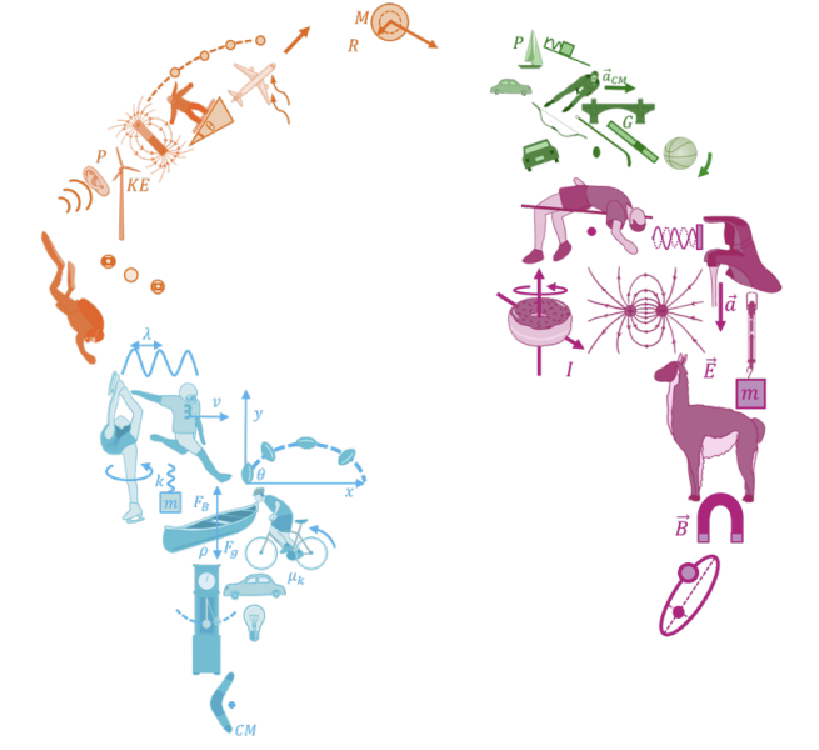
\includegraphics[width=4cm]{figures/BMDW/logo}
\end{textblock*}

\end{frame}

%%%%%%%%%%%%%TOC
\twocolframe{Outline}
  {\tableofcontents[sections={49,50}, subsectionstyle=show/show]\thispagestyle{empty}}
  {\tableofcontents[sections={51}, subsectionstyle=show/show]}
%%%%%%%%%%%%%%%%%%%%%%%%%







%%%%%%%%%%%%%%%%%%%%%%%%%%%%%%%%
\section{Defining Electric Potential}
\label{sec:definingelectricpotential}
\title{Defining Electric Potential}


%%%%%%%%%%%%%%%%%%%%%%%%%
\begin{frame}
\titlepage
\thispagestyle{empty}
\end{frame}

%%%%%%%%%%%%%%%



\subsection{Recall: work-energy theorem}
\label{subsec:recallworkenergytheorem}
\begin{frame}{Recall: Work-Energy Theorem}
If net work is performed on a particle in going from 1 to 2, that work is the change in kinetic energy:
\begin{align*}
W^{net}=\int_{\vec r_1}^{\vec r_2}\vec F^{net}\cdot d\vec r = K_2-K_1 = \Delta K = \frac{1}{2} m v_2^2 -\frac{1}{2}mv_1^2
\end{align*}
Remember, this was the whole reason for defining kinetic energy. We
defined kinetic energy because the difference in it is the net work done.
\end{frame}



%%%%%%%%%%%%%%%%%%%%%%%%%%%%%%
\subsection{Defining potential for conservatives forces}
\label{subsec:definingpotentialforconservatiesforces}
\begin{bulletframe}{For conservative forces, define potential
energy}
\item Calculating work can be complicated, as we have to evaluate the integral over the 3-dimensional path over which the force was applied.
\item However, if the work does not depend on the path taken, we can define a scalar function of position, $U(\vec r)$, ``potential energy'', that we evaluate at the end points of the path to calculate the work done by a specific force:
\begin{align*}
W=\int_{\vec r_1}^{\vec r_2}\vec F\cdot d\vec r =-\left[ U(\vec r_2)-U(\vec r_1) \right] = -\Delta U 
\end{align*}
\item Why the minus sign?
\only<2>{ Conservation of energy!
\begin{align*}
W^{net}= \Delta K = -\Delta U \;\;\rightarrow\;\; \Delta K + \Delta U = 0
\end{align*}
}
\end{bulletframe}


%%%%%%%%%%%%%%%%%%%%%%%%%%%%%%
\subsection{Defining a function for electrical potential energy}
\label{subsec:definingafunctionforelectricalpotentialenergy}
\begin{frame}{Defining a function for electrical potential energy}
\begin{itemize}
\item As a test case, use a ``fixed'' charge $+Q$ at the origin, and calculate the work done by the electric force on a positive charge $+q$ in going from: $\vec r_1$ to $\vec r_2$
\item Analogy with gravity: Use a fixed mass, $M$, at the origin, and calculate the work done by gravity on a mass, $m$, in going from position $\vec r_1$ to position $\vec r_2$
\item Choose a path that is always parallel to electric force.
%\capfig{0.6}{figures/potential}{Determining the work done on charge $q$ in going from $\vec r_1$ to $\vec r_2$}
\begin{center}
\begin{tikzpicture}
\tikzmath{
\L=5;
}
\scalebox{1}{

\coordinate (M) at (0,0);
\coordinate (mA) at (0.2*\L, 0);
\coordinate (mB) at (0.8*\L, 0);
\coordinate (mid) at ($(mA)!0.5!(mB)+(0,0.5)$);

\draw[-latex,line width=1.5] (0,0) -- (\L,0) node[below]{$r$};

\fill (M) circle (0.25) node[above=10pt]{$+Q$} node[below=10pt]{$0$};
\fill (mA) circle (2pt) node[below=5pt]{$r_1$};
\fill (mB) circle (2pt) node[below=5pt]{$r_2$};

\fill (mid) circle (3pt) node[left=3pt]{$+q$};
\draw[-latex, line width=1.5] (mid) -- +(1,0) node[above]{$\vec F_E(r)=k\frac{Qq}{r^2}\hat r$};
\draw[-latex, line width=1.5, color=myred] ($(mA)!0.5!(mB)$) -- +(0.75,0) node[below]{$d\vec r$};
}
\end{tikzpicture}
\captionof*{figure}{\textit{Determining the work done on charge $q$ in going from $\vec r_1$ to $\vec r_2$}}
\end{center}
\end{itemize}
\end{frame}




%%%%%%%%%%%%%%%%%%%%%%%%%%%%%%
\begin{frame}{Defining a function for electrical potential energy}
\vspace{-0.25cm}
\begin{center}
\begin{tikzpicture}
\tikzmath{
\L=5;
}
\scalebox{1}{

\coordinate (M) at (0,0);
\coordinate (mA) at (0.2*\L, 0);
\coordinate (mB) at (0.8*\L, 0);
\coordinate (mid) at ($(mA)!0.5!(mB)+(0,0.5)$);

\draw[-latex,line width=1.5] (0,0) -- (\L,0) node[below]{$r$};

\fill (M) circle (0.25) node[above=10pt]{$+Q$} node[below=10pt]{$0$};
\fill (mA) circle (2pt) node[below=5pt]{$r_1$};
\fill (mB) circle (2pt) node[below=5pt]{$r_2$};

\fill (mid) circle (3pt) node[left=3pt]{$+q$};
\draw[-latex, line width=1.5] (mid) -- +(1,0) node[above]{$\vec F_E(r)=k\frac{Qq}{r^2}\hat r$};
\draw[-latex, line width=1.5, color=myred] ($(mA)!0.5!(mB)$) -- +(0.75,0) node[below]{$d\vec r$};
}
\end{tikzpicture}
\captionof*{figure}{\textit{Determining the work done on charge $q$ in going from $\vec r_1$ to $\vec r_2$}}
\end{center}
%\capfig{0.3}{figures/potential}{Determining the work done on charge $q$ moving in a straight line.}
Calculate the work done on charge $q$ in going from $\vec r_1$ to $\vec r_2$:
\begin{align*}
W&=\int_{\vec r_1}^{\vec r_2}\vec F\cdot d\vec r = \int_{\vec r_1}^{\vec r_2}q\vec E\cdot d\vec r =kQq\int_{ r_1}^{r_2}\frac{1}{r^2}dr\\
&=kQq\left[ \frac{1}{r_1}-\frac{1}{r_2} \right] = -\Delta U = U_1 - U_2
\end{align*}
Define the potential energy function as (by inspection):
\begin{align*}
\boxed{U(r) = k\frac{Qq}{r} \textcolor{red}{+C}}
\end{align*}
\end{frame}


%%%%%%%%%%%%%%%%%%%%%%%%%%%%%%
\subsection{Choosing C}
\label{subsec:choosingC}
\begin{frame}{Choosing the constant, $C$}
\begin{align*}
U(r) = k\frac{Qq}{r} +C
\end{align*}
A simple and convenienent choice is $C=0$. This implies that the potential energy of $q$, when it is infinitely far away from $Q$, is zero. It makes sense, but is ulimately meaningless, since \textbf{only differences in potential energy are meaningful}.
\begin{align*}
\boxed{U(r) = k\frac{Qq}{r}}
\end{align*}
\end{frame}

%%%%%%%%%%%%%%%%%%%%%%%%%%%%%%


%%%%%%%%%%%%%%%%%%%%%%%%%%%%%%
\begin{frame}{What if $q$ is negative?}
Repeat the same exercise if the charge $q$ is negative:
\begin{align*}
W&=\int_{\vec r_1}^{\vec r_2}\vec F\cdot d\vec r = \int_{\vec r_1}^{\vec r_2}q\vec E\cdot d\vec r = q\int_{\vec r_1}^{\vec r_2}\vec E\cdot d\vec r =kQq\left[ \frac{1}{r_1}-\frac{1}{r_2} \right] = -\Delta U = U_1 - U_2
\end{align*}
Math is the same since $q$ factors out! That’s the whole point of defining the electric field!
\begin{align*}
\boxed{U(r) = k\frac{Qq}{r} +C}
\end{align*}
The product $qQ$ will take into account that the force changed direction (and thus the sign of the work being done depends on whether $qQ$ is positive or negative).
\end{frame}



%%%%%%%%%%%%%%%%%%%%%%%%%%%%%%
\subsection{Electric potential, $V$}
\label{subsec:electricalpotentialv}
\twocolframesf{Electric potential, $V$}
{
\begin{itemize}
\item We defined \textbf{electric field},$ \vec E$ , so that we could easily calculate the force on a charge $q$ of any sign. Electric field is \textit{force per unit charge}:
\begin{align*}
\vec F = q \vec E
\end{align*}
\item We do the same thing for potential energy! We define \textbf{electric potential}, $V$, as the \textit{potential energy per unit charge}:
\begin{align*}
U = q V
\end{align*}
\end{itemize}
}{
For a point charge, we have:
\begin{align*}
\vec F = k\frac{qQ}{r^2}\hat r \rightarrow \vec E = \frac{\vec F}{q}=k\frac{Q}{r^2}\hat r
\end{align*}
and:
\begin{align*}
U = k\frac{Qq}{r} \rightarrow V =\frac{U}{q}= k\frac{Q}{r}
\end{align*}
}

%%%%%%%%%%%%%%%%%%%%%%%%%%%%%%

%%%%%%%%%%%%%%%%%%%%%%%%%%%%%%

%%%%%%%%%%%%%%%%%%%%%%%%%%%%%%
\begin{bulletframe}{Properties of electric potential}
\item Just like potential energy, only difference in potentials are meaningful:
\begin{align*}
\Delta U &= q \Delta V\\
\Delta V &= \frac{\Delta U}{q}
\end{align*}
\item Electric potential (like potential energy) is a \textbf{scalar function of position}.
\item Potential energy relates to a specific charge, whereas potential relates to the potential energy that any charge would have.
\item \textbf{Voltage is a difference in potentials} ($\Delta V$ is a voltage). Saying that ``something is at voltage of \SI{200}{V}'' necessarily implies \textit{relative} to something else (e.g. ground). 
\end{bulletframe}

%%%%%%%%%%%%%%%%%%%%%%%%%%%%%%


%%%%%%%%%%%%%%%%%%%%%%%%




%%%%%%%%%%%%%%%%%%%%%%%%%%%%%%
\twocolframesf{Electric potential, $V$}
{
\begin{itemize}
\item We defined \textbf{electric field}, $\vec E$, so that we could easily calculate the force on a charge $q$ of any sign. Electric field is \textit{force per unit charge}:
\begin{align*}
\vec F = q \vec E
\end{align*}
\item We do the same thing for potential energy! We define \textbf{electric potential}, $V$, as \textit{potential energy per unit charge}:
\begin{align*}
U = q V
\end{align*}
\end{itemize}
}{
For a point charge, we have:
\begin{align*}
\vec F = k\frac{qQ}{r^2}\hat r \rightarrow \vec E = \frac{\vec F}{q}=k\frac{Q}{r^2}\hat r
\end{align*}
and:
\begin{align*}
U = k\frac{Qq}{r} \rightarrow V =\frac{U}{q}= k\frac{Q}{r}
\end{align*}
}

%%%%%%%%%%%%%%%%%%%%%%%%%%%%%%


%%%%%%%%%%%%%%%%%%%%%%%%%%%%%%
\twocolframesf{Electric potential}
{
\only<1,2>{
 \begin{itemize}
 \item Only differences in potential are meaningful, and they correspond to differences in potential energy
 \item All charges, if left free, will try to decrease their potential energy
 \item For a positive charge, potential energy increases with increasing potential
 \item For a negative charge, potential energy decreases with increasing potential
 \end{itemize}

 }
\only<3>{
 \vspace{3cm}
 It doesn't matter where you set $V=0$ to, as long as you're consistent!
 }
}
{
\only<1>{
\vspace{-0.5cm}
\begin{center}
\begin{tikzpicture}
\tikzmath{
\L=2.5;
}
\scalebox{1}{

\begin{scope}
%\clip (-1.3*\L,-1.3*\L) rectangle (1.3*\L,1.3*\L);
\foreach \th in {0,30,...,330}{
\draw (0,0) -- (\th:1.1*\L);
\draw[latex-] (\th:0.6*\L) -- +(\th:-0.2);
}
\end{scope}
\fill[color=myblue!80] (0,0) circle (5pt);
\node[color=white] at (0,0){+};

\draw[dotted, color=myred, line width=1.5] (0,0) circle(\L);
\draw[dotted, color=myred, line width=1.5] (0,0) circle(\L/2);
\draw[dotted, color=myred, line width=1.5] (0,0) circle(\L/3);
\draw[dotted, color=myred, line width=1] (0,0) circle(\L/4);
\draw[dotted, color=myred, line width=1] (0,0) circle(\L/5);
\draw[dotted, color=myred, line width=1] (0,0) circle(\L/6);
\draw[dotted, color=myred, line width=1] (0,0) circle(\L/7);

\node[above,color=myred] at (75:\L){\SI{10}{V}};
\node[above,color=myred] at (70:\L/2){\SI{20}{V}};
\node[above,color=myred] at (70:\L/3){\scriptsize \SI{30}{V}};
}
\end{tikzpicture}
\captionof*{figure}{\textit{Point charge: electric field and potential.}}
\end{center}
%\capfig{0.8}{figures/fig2}{Point charge: electric field and potential}
}
\only<2->{
\begin{center}
\begin{tikzpicture}
\tikzmath{
\h=6;
}
\scalebox{1}{
\draw[-latex,line width=2] (0,0) -- +(0,\h)node[midway, above,rotate=90]{Electric potential};
\draw[-latex,line width=2,color=myred] (1,0) -- +(0,\h)node[midway, above,rotate=90]{Potential energy of $+Q$};
\draw[latex-,line width=2,color=myblue!80] (2,0) -- +(0,\h)node[midway, above,rotate=90]{Potential energy of $-Q$};
\only<3>{
\draw[line width=2] (-1,1) node[left]{$V=0$} -- (3,1);
}
}
\end{tikzpicture}
\captionof*{figure}{\textit{Potential and potential energy.}}
\end{center}
}
}



%%%%%%%%%%%%%%%%%%%%%%%%%%%%%%
\twocolframe{Potential and Potential Energy}
{
\vspace{-0.25cm}
\textbf{Gravitational Force}
{\footnotesize 
\begin{itemize}
\item Force:
\begin{align*}
\vec F = \frac{GMm}{r^2}\hat r
\end{align*}

\item Field (force per unit mass) near \textbf{point mass $M$}:
\begin{align*}
\vec g = \frac{GM}{r^2}\hat r
\end{align*}

\item Potential energy near \textbf{point mass $M$}:
\begin{align*}
U(r) = -\frac{GMm}{r}+C=-\int \vec F\cdot d \vec r
\end{align*}

\item ``Potential'' \textbf{from point mass $M$} (potential energy per unit mass):
\begin{align*}
V(r) = -\frac{GM}{r}+C=-\int \vec g\cdot d \vec r
\end{align*}
\end{itemize}
}
}
{
\vspace{-0.25cm}
\textbf{Electric Force}
{\footnotesize 

\begin{itemize}
\item Force:
\begin{align*}
\vec F = \frac{kQq}{r^2}\hat r
\end{align*}

\item Field (force per unit \textit{charge}) near \textbf{point \textit{charge} $Q$}:
\begin{align*}
\vec E = \frac{kQ}{r^2}\hat r
\end{align*}

\item Potential energy near \textbf{point \textit{charge} $Q$}:
\begin{align*}
U(r) = -\frac{kQq}{r}+C=-\int \vec F\cdot d \vec r
\end{align*}

\item ``Potential'' \textbf{from point \textit{charge} $Q$} (potential energy per unit \textit{charge}):
\begin{align*}
V(r) = -\frac{kQ}{r}+C=-\int \vec E\cdot d \vec r
\end{align*}
\end{itemize}
}
}

%%%%%%%%%%%%%%%%%%%%%%%




%%%%%%%%%%%%%%%%%%%%%%%%%%%%%%%%
\section{Calculating Electric Potential}
\label{sec:calculatingelectricpotential}
\title{Calculating Electric Potential}


%%%%%%%%%%%%%%%%%%%%%%%%%
\begin{frame}
\titlepage
\thispagestyle{empty}
\end{frame}

%%%%%%%%%%%%%%%






%%%%%%%%%%%%%%%%%%%%%%%%%%%%%%
\begin{frame}{Calculating electric potential}
Work done by the force gives potential energy:
\begin{align*}
W&=\int_{\vec r_1}^{\vec r_2}\vec F\cdot d\vec r = \int_{\vec r_1}^{\vec r_2}q\vec E\cdot d\vec r = \textcolor{red}{q}\int_{\vec r_1}^{\vec r_2}\vec E\cdot d\vec r = -\Delta U 
\end{align*}
Doing this per charge, gives electric potential
\begin{align*}
-\Delta V = \frac{-\Delta U}{q}=\int_{\vec r_1}^{\vec r_2}\vec E\cdot d\vec r 
\end{align*}
Electric potential is to electrical potential energy what electric field is to electric force:
\begin{align*}
\Delta U &= -\int_{\vec r_1}^{\vec r_2} \textcolor{red}{\vec F}\cdot d\vec r\\
\Delta V &= -\int_{\vec r_1}^{\vec r_2} \textcolor{red}{\vec E}\cdot d\vec r
\end{align*}
\end{frame}

%%%%%%%%%%%%%%%%%%%%%%%%%%%%%%

%%%%%%%%%%%%%%%%%%%%%%%%%%%%%
\subsection{Methods of determining electric potential}
\label{subsec:methodsofdeterminingelectricpotential}
\twocolframest{Two methods to determine electric potential}
{
\begin{enumerate}
\item \textbf{Use the electric field} and integrate it (if you already know the electric field):
\begin{align*}
\Delta V &= (V_2-V_1) = -\int_{\vec r_1}^{\vec r_2} \vec E\cdot d\vec r\\
V(\vec r)&= -\int \vec E \cdot d\vec r
\end{align*}
\item \textbf{Model as a collection of point charges} and sum the potentials (\textcolor{myred}{Make sure they share the location of \SI{0}{V}!}):
\begin{align*}
dV&=\frac{kdq}{r}\\
\therefore V &= \int dV = k \int \frac{dq}{r}
\end{align*}
\end{enumerate}
}
{
\begin{block}{Using the $E$-field}
This is what we did to determine the potential near a point charge $Q$
\end{block}
\vspace{2cm}
\begin{block}{Summing the potentials}
This is analogous to how we calculate the electric field for a distributed charge, but much easier since potential is a scalar!
\end{block}
}

%%%%%%%%%%%%%%%%%%%%%%%%%%%%%%



\subsection{Electric potential near a point charge}
\label{subsec:electricpotentialnearapointcharge}
\begin{frame}{Electric potential near a point charge, $Q$}

\begin{itemize}
\item We can calculate the potential energy function from the anti-derivative:
\begin{align*}
V(r) &= -\int \textcolor{red}{\vec E}\cdot d\vec r = -\int k\frac{Q}{r^2}dr = k\frac{Q}{r}+C\\
\end{align*}
\item \textbf{If we define zero potential energy at infinity ($C = 0$)}, then this also corresponds to zero electric potential, and we can define electric potential from a point charge as:
\begin{align*}
 V(r) =k\frac{Q}{r}
\end{align*}
\end{itemize}
\end{frame}
%%%%%%%%%%%%%%%%%%%%%%%%%%%%%%%%
\twocolframest{Electric potential energy near point charge, $Q$}
{
\begin{itemize}
\item Found the potential energy of q a distance r from Q:\\
\begin{align*}
U(r) = \frac{kQq}{r}+C
\end{align*}
\item Convenient choice is $C=0$
\item This means that we explicitly define $U(r)=0$ when $r\to\infty$:
\begin{align*}
\boxed{U(r) = \frac{kQq}{r}}
\end{align*}

\end{itemize}
}
{
\begin{center}
\begin{tikzpicture}
\tikzmath{
\L=2;
\R=0.25;
}
\scalebox{1}{

\fill[color=myblue!80] (0,0) circle(\R) node[above=5pt,color=black]{$Q$};
\fill[color=myblue!80] (\L,0) circle(\R/2) node[above=5pt,color=black]{$q$};
\draw[latex-latex] (0,0) -- (\L,0) node[midway,below]{$r$};
}
\end{tikzpicture}
\captionof*{figure}{\textit{Point charges separated by distance, $r$.}}
\end{center}
}



%%%%%%%%%%%%%%%%%%%%%%%%%%%%%%
\subsection{Potential from a ring of charge}
\label{subsec:potentialfromaringofcharge}
\twocolframesf{Potential from a ring of charge, along symmetry axis}
{
\begin{itemize}
\item Break it up into many small point charges, $dq$.
\item Write the potential from a $dq$:
\begin{align*}
dV&=\frac{kdq}{r}=\frac{kdq}{\sqrt{R^2+x^2}}
\end{align*}
\item Sum the potentials (integrate):
\begin{align*}
\therefore V &= \int dV = \int_0^Q \frac{kdq}{\sqrt{R^2+x^2}} = \frac{kQ}{\sqrt{R^2+x^2}}
\end{align*}
\end{itemize}
\only<1>{
\begin{alertblock}{Careful!}
This only works if all the potentials, $dV$, have the same locations defined for \SI{0}{V} (namely, at infinity, since we chose $C=0$).
\end{alertblock}
}
\only<2>{
\begin{block}{Easy integrand!}
We don't need to express $dq$ with a position variable (e.g. $dq=\lambda R d\theta$) since all quantities in the integrand are constants! But you should try to convince yourself you'll get the same answer!
\end{block}
}
}
{
%\capfig{0.5}{figures/potential_ring}{A point charge, $dq$, on the ring}
\begin{center}
\begin{tikzpicture}
\tikzmath{
\L=2.5;
\R=0.5*\L;
\thperp=45;
\Px=0.5*\L;
\dtheta=20;
}
\scalebox{1}{

\draw[-latex] (0,0) -- +(\L,0) node[below]{$x$};
\draw[-latex] (0,0) -- +(0,\L) node[left]{$z$};
\draw[-latex,dashed] (0,0) -- +(\thperp:0.75*\L) node[right]{$y$};

\draw[line width=1.5] (0,\R) arc(90:270:{\R/4} and {\R});
\draw[line width=1] (0,\R) arc(90:-90:{\R/4} and {\R});

\node[above left] at (0,\R) {$Q$};
\node[above, color=myred] at (0.5*\Px,0) {$x$};
\fill (\Px,0) circle (2pt) node[above]{$P$};
\draw[color=myred, line width=1.5] (270+\dtheta:{\R/4} and {\R}) arc (270+\dtheta:270-\dtheta:{\R/4} and {\R}) node[midway,below]{$dq$};

\draw[color=myred, line width=1.5, dotted] (270:{\R/4} and {\R}) -- (\Px,0) node[midway,right]{$\sqrt{R^2+r^2}$};
\only<1>{
\draw[dotted, line width=1] (0,0) -- (225:{\R/4} and {\R}) node[midway,right=-2pt]{$R$};
}
\only<2>{

\draw[color=myred] (0,0) -- (270+\dtheta:{\R/4} and {\R}) ;
\draw[color=myred] (0,0) -- (270-\dtheta:{\R/4} and {\R}) ;
\draw[-latex, color=myred] (-\R/2,-\R/2) node[left]{$d\theta$} -- (0,-\R/2);
}
}
\end{tikzpicture}
\captionof*{figure}{\textit{A point charge, $dq$, on a ring of radius, $R$.}}
\end{center}

}


%%%%%%%%%%%%%%%%%%%%%%%%%%%%%%
\twocolframesf{Potential from a disk carrying surface charge, $\sigma$}
{
\begin{itemize}
\item Break up the disk into \textcolor{red}{small rings} of charge, $\textcolor{red}{dq}$, and radius, $\textcolor{red}{r}$. Each ring has an area $dA$:
\begin{align*}
dq = \sigma dA = \sigma 2\pi r dr
\end{align*}
\item Write the potential from $dq$ (using our previous result):
\begin{align*}
dV = \frac{kdq}{\sqrt{r^2+x^2}}=\frac{k\sigma 2\pi r dr}{\sqrt{r^2+x^2}}
\end{align*}
\item Sum the potentials:
\begin{align*}
\therefore V = \int dV = 2\pi k \sigma \int_0^R \frac{ r}{\sqrt{r^2+x^2}}dr
\end{align*}
\end{itemize}
}
{

\begin{center}
\begin{tikzpicture}
\tikzmath{
\L=2.5;
\R=0.9*\L;
\Rdq=0.6*\R;
\thperp=45;
\Px=0.5*\L;
\dtheta=20;
}
\scalebox{1}{

\draw[-latex] (0,0) -- +(\L,0) node[below]{$x$};
\draw[-latex] (0,0) -- +(0,1.1*\L) node[left]{$z$};
\draw[-latex,dashed] (0,0) -- +(\thperp:0.75*\L) node[right]{$y$};

\fill[color=myblue!60,opacity=0.3] (0,0) circle ({\R/4} and {\R});

\draw[line width=3.5,color=myred] (0,\Rdq) arc(90:270:{\Rdq/4} and {\Rdq});
\draw[line width=2.5,color=myred] (0,\Rdq) arc(90:-90:{\Rdq/4} and {\Rdq});


\fill (\Px,0) circle (2pt) node[above]{$P$};
\node[above, color=myred] at (0.5*\Px,0) {$x$};

\draw[dotted, line width=1, color=myred] (0,0) -- (225:{\Rdq/4} and {\Rdq}) node[midway,right=-2pt]{$r$};

\draw[color=myred,line width=1, latex-] (0,-\Rdq+0.1) -- +(0,0.3);
\draw[color=myred,line width=1, latex-] (0,-\Rdq-0.1) -- +(0,-0.3);
\node[color=myred, right=5pt] at (0,-\Rdq){$dr$};
\node[right=5pt] at (0,\R) {$R$};
\node[above] at (0,-\R) {$\sigma$};
}
\end{tikzpicture}
\captionof*{figure}{\textit{A ring of charge $dq$ on a disk carrying surface charge $\sigma$. Think of unfolding the ring into a rectangle of length $2\pi r$ and height $dr$ to determine its area, $dA$.}}
\end{center}

}


%%%%%%%%%%%%%%%%%%%%%%%%%%%%%%



%%%%%%%%%%%%%%%%%%%%%%%%%%%%%%
\subsection{Getting $\vec E$ from $V$}
\label{subsec:gettingefromv}
\twocolframesf{What about $\vec E$ from $V$?}
{
\begin{itemize}
\item If we know the electric field vector, by using a scalar product ($q\vec E \cdot d\vec r$), we can find the electric potential (vector $\to$ scalar)
\item How do we go the other way (scalar $\to$ vector)?
\begin{itemize}
\item Based on the direction in which electric potential increases, we can \textbf{determine the direction of the field}.
\item Based on how quickly the potential changes, we can determine the \textbf{magnitude of the field}. 
\end{itemize}

\end{itemize}
}
{
\capfig{1}{figures/Potential/contours}{Contour lines on a map}
\begin{block}{Contour lines}
Lines (contours) of constant electric potential correspond to lines of constant electric potential energy. Just like lines of constant altitude correspond to lines of constant gravitational potential energy.
\end{block}
}



%%%%%%%%%%%%%%%%%%%%%%%%%%%%%%
\twocolframesf{$\vec E$ from $V$ in 1D}
{
\begin{itemize}
\item $V$ from $\vec E$:
\begin{align*}
V(x) = -\int E dx
\end{align*}
\item $\vec E$ from $V$
\begin{align*}
\therefore E(x) = -\frac{dV}{dx}=-k
\end{align*}
\item Electric potential is the (negative) anti-derivative of electric field (in 1D).
\item Electric field  is this the (negative) derivative of electric potential.
\end{itemize}

}
{
%\capfig{0.35}{figures/potential_linear}{Example of a linear potential}
\begin{center}
\begin{tikzpicture}
\tikzmath{
\h=4;
\L=3;
}
\scalebox{1}{

\draw[-latex, line width =1.5] (0,0) -- +(0,1.2*\h) node[left]{$x$};

\foreach \i in {0,0.1,...,1.1}{
 \draw[line width =1] (0.2,\i*\h) -- +(\L,0);
}

\node[above] at (\L/2,\h){$V(x)=kx$};
\node[right=5pt] at (\L,0){\SI{0}{V}};
\node[right=5pt] at (\L,0.5*\h){\SI{50}{V}};
\node[right=5pt] at (\L,\h){\SI{100}{V}};
}
\end{tikzpicture}
\captionof*{figure}{\textit{Example of a linear potential.}}
\end{center}
}


%%%%%%%%%%%%%%%%%%%%%%%%%%%%%%
\twocolframest{$\vec E$ from $V$ in 3D}
{
\vspace{-0.5cm}
\begin{itemize}
\item $V$ from $\vec E$:
\begin{align*}
V(\vec r)= V(x,y,z) = -\int \vec E \cdot  d\vec r
\end{align*}
\item $\vec E$ from $V$
\begin{align*}
E_x &= -\frac{\partial V}{\partial x}\\
E_y &= -\frac{\partial V}{\partial y}\\
E_z &= -\frac{\partial V}{\partial z}
\end{align*}
\item In 3D, we need to know how the potential changes (its derivatives) in each direction. Those (partial) derivatives are the 3 components of the electric field!
\end{itemize}

}
{
\begin{block}{Different Notation}
The electric field is the (negative) gradient of the electric potential:
\begin{align*}
\vec E &= -\nabla V\\
&=-\left( \frac{\partial V}{\partial x} \hat x + \frac{\partial V}{\partial y}\hat y+\frac{\partial V}{\partial z}\hat z\right)
\end{align*}
\end{block}
}


%%%%%%%%%%%%%%%%%%%%%%%%%%%%%%





%%%%%%%%%%%%%%%%%%%%%%%%%%%%%%%%
\section{Application}
\label{sec:application}
\title{Application}


%%%%%%%%%%%%%%%%%%%%%%%%%
\begin{frame}
\titlepage
\thispagestyle{empty}
\end{frame}

%%%%%%%%%%%%%%%



%%%%%%%%%%%%%%%%%%%%%%%%
\subsection{Gradient vector review}
\label{subsec:gradientvectorreview}
\twocolframe{Recall the gradient vector}
{
\begin{itemize}
\item From the partial derivatives, we know how the function changes along the $x$ and $y$ directions
\item The gradient tells us the direction in which the function changes the fastest (in which direction the slope is the steepest)
\item It is a vector whose magnitude tells us how fast the function is changing in the direction of maximal change.
\begin{align*}
\nabla f(x,y) &= \frac{\partial f}{\partial x} \hat x + \frac{\partial f}{\partial y}\hat y\\
&=2x\hat x - 4y \hat y = (-4,8)
\end{align*}
\end{itemize}
}
{
\begin{tikzpicture}[scale=0.8]

\begin{axis}[
  colormap/viridis,  
  view = {40}{40},
	xmax = 5,
	xmin = -5,
	ymax = 5, 
	ymin = -5, 
	zmax = 50, 
	zmin = -50,
	xtick = {-4,-2,0,2,4},
	ytick = {-4,-2,0,2,4},
	ztick = {-40,-20,0,20,40},
	xlabel={x},
	ylabel={y},
	title={$f(x)=x^2-2y^2$},
	grid]
	

\addplot3 [
	domain=-5:5,
	domain y = -5:5,
	samples = 20,
	samples y = 20,
	surf,
	shader =faceted interp] {x^2 -2*y^2};
	
\node[label={P(-2,-2,-4)}] at (-2,-2,-4) {};
\draw plot [mark=*, mark size=2] coordinates{(-2,-2,-4)}; 

\end{axis}

\end{tikzpicture}
\captionof*{figure}{\textit{A point, $P$, is on the surface given by $f(x,y)=x^2-2y^2$.}}
}


%%%%%%%%%%%%%%%%%%%%%%%%%%%%%%
\twocolframe{Recall the gradient vector}
{
\begin{itemize}
\item From the partial derivatives, we know how the function changes along the $x$ and $y$ directions
\item The gradient tells us the direction in which the function changes the fastest (in which direction the slope is the steepest)
\item It is a vector whose magnitude tells us how fast the function is changing in the direction of maximal change.
\begin{align*}
\nabla f(x,y) &= \frac{\partial f}{\partial x} \hat x + \frac{\partial f}{\partial y}\hat y\\
&=2x\hat x - 4y \hat y = (-4,8)
\end{align*}
\end{itemize}
}
{
\begin{tikzpicture}[scale=0.8]
\usetikzlibrary {arrows.meta} 
\begin{axis}[
  colormap/viridis,  
  view = {40}{40},
	xmax = 5,
	xmin = -5,
	ymax = 5, 
	ymin = -5, 
	zmax = 50, 
	zmin = -50,
	xtick = {-4,-2,0,2,4},
	ytick = {-4,-2,0,2,4},
	ztick = {-40,-20,0,20,40},
	xlabel={x},
	ylabel={y},
	title={$f(x)=x^2-2y^2$},
	grid]
	

\addplot3 [
	domain=-5:5,
	domain y = -5:5,
	samples = 20,
	samples y = 20,
	mesh,
	%fill opacity=0.5,
	shader =faceted interp] {x^2 -2*y^2};
	
\draw[line width=2pt,dotted] (-2,-2,-50) -- (-2,-2,-4)	;
\node[label={P(-2,-2,-4)}] at (-2,-2,-4) {};
\draw plot [mark=*, mark size=2] coordinates{(-2,-2,-4)}; 
\draw[line width=2pt,red,-{Stealth[round]}] (-2,-2,-50)--(-3.5,1,-50) node[right]{$\nabla f$};

\end{axis}

\end{tikzpicture}
\captionof*{figure}{\textit{A vector parallel to the gradient vector is projected in the $xy$-plane. It points in the direction of most rapid increase.}}
}


\begin{bulletframe}{Gradient in physics}
\item The \textbf{gradient of the potential energy} tells us in which direction the \textbf{corresponding force} is exerted. The force is exerted in the opposite direction of the gradient vector (the force is exerted in the direction opposite to that which potential energy increases).
\begin{itemize}
\item Think of a contour map in the context of gravity. The contours are regions of constant elevation (namely, constant gravitational potential energy).
\end{itemize}
\item The \textbf{gradient of the electric potential} tells us in which direction the \textbf{corresponding electric field} is. The field is in the opposite direction of  the gradient vector.
\end{bulletframe}

%%%%%%%%%%%%%%%%%%%%%%%%%%




%%%%%%%%%%%%%%%%%%%%%%%%%%%%%%%%
\subsection{Electric potential summary}
\label{subsec:electricpotentialsummary}
\begin{bulletframe}{Summary: Electric Potential}
 \item We started with Coulomb’s Law for the \textbf{electric force vector} between 2 points charges: $\vec F$
 \item We defined the \textbf{electric field vector}, which is independent of the ``test'' charge, $q$: $\vec F=q\vec E$
 \item Knowing that the force is conservative, we defined a (scalar) \textbf{potential energy function}: $U(\vec r)$
 \item We defined the \textbf{electric potential function}, which is independent of the test charge, $q$: $U(\vec r) = q V(\vec r)$
 \item[$\rightarrow$] We can now describe the motion of electric charges using scalar quantities (electric potential and electric potential energy).
 \item[$\rightarrow$] Instead of an electric force vector acting in certain direction, you can think of charges moving to regions of space where they will lower the electric potential energy.
\end{bulletframe}



%%%%%%%%%%%%%%%%%%%%%%%%%%%%%%


%%%%%%%%%%%%%%%%%%%%%%%%%%%%%%
\subsection{Equipotential surfaces}
\label{subsec:equipotentialsurfaces}
\twocolframesf{Equipotential surfaces}
{
\begin{itemize}
  \item Electric potential is a scalar function of position, $V(x,y,z)$.
  \item Electric potential gives the electric potential energy of a charge at a given position.
  \item \textbf{Equipotential surfaces} are regions of space where electric potential is constant.
  \item The electric field does not do work along an equipotential surface.
  \item Conductors are always equipotentials (the net field inside a conductor must be zero in electrostatics, so the potential cannot change inside a conductor). 
\end{itemize}
}
{
\begin{center}
\begin{tikzpicture}
\tikzmath{
\L=2;
}
\scalebox{1}{

\begin{scope}
%\clip (-1.3*\L,-1.3*\L) rectangle (1.3*\L,1.3*\L);
\foreach \th in {0,30,...,330}{
\draw (0,0) -- (\th:1.1*\L);
\draw[latex-] (\th:0.6*\L) -- +(\th:-0.2);
}
\end{scope}
\fill[color=myblue!80] (0,0) circle (5pt);
\node[color=white] at (0,0){+};

\draw[dotted, color=myred, line width=1.5] (0,0) circle(\L);
\draw[dotted, color=myred, line width=1.5] (0,0) circle(\L/2);
\draw[dotted, color=myred, line width=1.5] (0,0) circle(\L/3);
\draw[dotted, color=myred, line width=1] (0,0) circle(\L/4);
\draw[dotted, color=myred, line width=1] (0,0) circle(\L/5);
\draw[dotted, color=myred, line width=1] (0,0) circle(\L/6);
\draw[dotted, color=myred, line width=1] (0,0) circle(\L/7);

}
\end{tikzpicture}
\captionof*{figure}{\textit{For a point charge, equipotential surfaces consist in concentric spheres; the electric field foes no work along one of these surfaces.}}
\end{center}



}




%%%%%%%%%%%%%%%%%%%%%%%%%%%%%%
\twocolframesf{Equipotential surfaces}
{
\begin{itemize}
  \item Since they are regions of constant electric potential energy, the electric field does no work when moving along an equipotential
  \item The equipotential surfaces are always perpendicular to the electric field lines:
  \begin{align*}
  W = \vec F \cdot \vec d = Fd\cos\theta
  \end{align*}
  \item[$\rightarrow$]  Electric field is always perpendicular to surface of the conductor

\end{itemize}
}
{
\begin{center}
\begin{tikzpicture}
\tikzmath{
\xe=-2;%Coordinates of first mass/charge (Earth)
\ye=0;
\xm=2;%Coordinates of first mass/charge (Moon)
\ym=0;
\mee=1;% Mass/charge of first mass (Earth)
\mmm=0.6;% Mass/charge of first mass (Earth)
\dl=0.1;%scale factor to advance along the field line
\n=35;%number of points to find in the line (make as small as possible to reach the point you want!)
\nequi=60;
}

\scalebox{1}{
%Top field lines (xst is the starting x position of the field line)
\foreach \xst in {-2.8,-2.4,...,2.4}{
  \tikzmath{
  \yst=1.7; %all field lines start at yst
  \x=\xst;
  \y=\yst;
  %
  %generate points on the line (keeps finding the next point)
  int \i;
  %note that this also creates \mypairx and \mypairy!
  coordinate \mypair;
  for \i in {1,...,\n}{
    %First mass (earth)
    \re=(\x-\xe)*(\x-\xe)+(\y-\ye)*(\y-\ye)+0.0001;
    \Fex=\mee*(\x-\xe)/\re;
    \Fey=\mee*(\y-\ye)/\re;
    %Second mass (moon)
    \rm=(\x-\xm)*(\x-\xm)+(\y-\ym)*(\y-\ym)+0.0001;
    \Fmx=\mmm*(\x-\xm)/\rm;
    \Fmy=\mmm*(\y-\ym)/\rm;
    %Total force:
    \Fx=\Fex+\Fmx;
    \Fy=\Fey+\Fmy;
    \Fn=sqrt(\Fx*\Fx+\Fy*\Fy)+0.0001;
    \dx=\Fx/\Fn*\dl;
    \dy=\Fy/\Fn*\dl; 
    \x=\x-\dx;
    \y=\y-\dy;
    \mypair{\i}=(\x,\y);
    };
  }
  %Draw that field line
  \foreach \i in {2,...,\n}{
    \tikzmath{
    int \im;
    \im=\i-1;
    }
    \draw (\mypair{\im}) -- (\mypair{\i});
    \ifthenelse{\im =5}{\draw[latex-] (\mypair{\im}) -- (\mypair{\i})}{};%draw arrow on the fifth point
  }

}%end of loop over x

%equipotential:
\foreach \yst in {0.5,0.75,1, 1.25}{
  \tikzmath{
  \xst=\xe;
  %\yst=0.75; %all field lines start at yst
  \x=\xst;
  \y=\yst;
  %
  %generate points on the line (keeps finding the next point)
  int \i;
  %note that this also creates \mypairx and \mypairy!
  coordinate \mypair;
  for \i in {1,...,\nequi}{
    %First mass (earth)
    \re=(\x-\xe)*(\x-\xe)+(\y-\ye)*(\y-\ye)+0.0001;
    \Fex=\mee*(\x-\xe)/\re;
    \Fey=\mee*(\y-\ye)/\re;
    %Second mass (moon)
    \rm=(\x-\xm)*(\x-\xm)+(\y-\ym)*(\y-\ym)+0.0001;
    \Fmx=\mmm*(\x-\xm)/\rm;
    \Fmy=\mmm*(\y-\ym)/\rm;
    %Total force:
    \Fx=\Fex+\Fmx;
    \Fy=\Fey+\Fmy;
    \Fn=sqrt(\Fx*\Fx+\Fy*\Fy)+0.0001;
    \dx=-\Fy/\Fn*\dl;
    \dy=\Fx/\Fn*\dl;
    \x=ifthenelse(\x>-2.001,\x-\dx,\x);
    \y=ifthenelse(\x>-2.001,\y-\dy,\y);
    \mypair{\i}=(\x,\y);
    };
  }
  %Draw that field line
  \foreach \i in {2,...,\nequi}{
    \tikzmath{
    int \im;
    \im=\i-1;
    }
    \draw[color=myred,dotted,line width=1.5] (\mypair{\im}) -- (\mypair{\i});
    //\ifthenelse{\im =5}{\draw[latex-] (\mypair{\im}) -- (\mypair{\i})}{};%draw arrow on the fifth point
  }

}%end of loop over x

%Bottom field lines
\foreach \xst in {-2.8,-2.4,...,2.4}{
  \tikzmath{
  \yst=-1.7;
  \x=\xst;
  \y=\yst;
  %
  %generate points on the line
  int \i;
  %note that this also creates \mypairx and \mypairy!
  coordinate \mypair;
  for \i in {1,...,\n}{
    %First mass (earth)
    \re=(\x-\xe)*(\x-\xe)+(\y-\ye)*(\y-\ye)+0.0001;
    \Fex=\mee*(\x-\xe)/\re;
    \Fey=\mee*(\y-\ye)/\re;
    %Second mass (moon)
    \rm=(\x-\xm)*(\x-\xm)+(\y-\ym)*(\y-\ym)+0.0001;
    \Fmx=\mmm*(\x-\xm)/\rm;
    \Fmy=\mmm*(\y-\ym)/\rm;
    %Total force:
    \Fx=\Fex+\Fmx;
    \Fy=\Fey+\Fmy;
    \Fn=sqrt(\Fx*\Fx+\Fy*\Fy)+0.0001;
    \dx=\Fx/\Fn*\dl;
    \dy=\Fy/\Fn*\dl;
    \x=\x-\dx;
    \y=\y-\dy;
    \mypair{\i}=(\x,\y);
     };
  }
  %Draw that field line
  \foreach \i in {2,...,\n}{
    \tikzmath{
      int \im;
      \im=\i-1;
    }
    \draw (\mypair{\im}) -- (\mypair{\i});
    \ifthenelse{\im =5}{\draw[latex-] (\mypair{\im}) -- (\mypair{\i})}{};
  }

}%end of loop over x


%equipotential:
\foreach \yst in {-0.25, -0.5,-0.75}{
  \tikzmath{
  \xst=\xm;
  %\yst=0.75; %all field lines start at yst
  \x=\xst;
  \y=\yst;
  %
  %generate points on the line (keeps finding the next point)
  int \i;
  %note that this also creates \mypairx and \mypairy!
  coordinate \mypair;
  for \i in {1,...,\nequi}{
    %First mass (earth)
    \re=(\x-\xe)*(\x-\xe)+(\y-\ye)*(\y-\ye)+0.0001;
    \Fex=\mee*(\x-\xe)/\re;
    \Fey=\mee*(\y-\ye)/\re;
    %Second mass (moon)
    \rm=(\x-\xm)*(\x-\xm)+(\y-\ym)*(\y-\ym)+0.0001;
    \Fmx=\mmm*(\x-\xm)/\rm;
    \Fmy=\mmm*(\y-\ym)/\rm;
    %Total force:
    \Fx=\Fex+\Fmx;
    \Fy=\Fey+\Fmy;
    \Fn=sqrt(\Fx*\Fx+\Fy*\Fy)+0.0001;
    \dx=-\Fy/\Fn*\dl;
    \dy=\Fx/\Fn*\dl;
    \x=ifthenelse((\x<2.001) && (\x>-2.001),\x-\dx,\x);
    \y=ifthenelse((\x<2.001) && (\x>-2.001),\y-\dy,\y);
    \mypair{\i}=(\x,\y);
    };
  }
  %Draw that field line
  \foreach \i in {2,...,\nequi}{
    \tikzmath{
    int \im;
    \im=\i-1;
    }
    \draw[color=myred,dotted,line width=1.5] (\mypair{\im}) -- (\mypair{\i});
  }

}%end of loop over x


%equipotential:
\foreach \yst in {0.75}{
  \tikzmath{
  \xst=\xm;
  %\yst=0.75; %all field lines start at yst
  \x=\xst;
  \y=\yst;
  %
  %generate points on the line (keeps finding the next point)
  int \i;
  %note that this also creates \mypairx and \mypairy!
  coordinate \mypair;
  for \i in {1,...,\nequi}{
    %First mass (earth)
    \re=(\x-\xe)*(\x-\xe)+(\y-\ye)*(\y-\ye)+0.0001;
    \Fex=\mee*(\x-\xe)/\re;
    \Fey=\mee*(\y-\ye)/\re;
    %Second mass (moon)
    \rm=(\x-\xm)*(\x-\xm)+(\y-\ym)*(\y-\ym)+0.0001;
    \Fmx=\mmm*(\x-\xm)/\rm;
    \Fmy=\mmm*(\y-\ym)/\rm;
    %Total force:
    \Fx=\Fex+\Fmx;
    \Fy=\Fey+\Fmy;
    \Fn=sqrt(\Fx*\Fx+\Fy*\Fy)+0.0001;
    \dx=-\Fy/\Fn*\dl;
    \dy=\Fx/\Fn*\dl;
    \x=ifthenelse((\x<2.001) && (\x>-2.001),\x+\dx,\x);
    \y=ifthenelse((\x<2.001) && (\x>-2.001),\y+\dy,\y);
    \mypair{\i}=(\x,\y);
    };
  }
  %Draw that field line
  \foreach \i in {2,...,\nequi}{
    \tikzmath{
    int \im;
    \im=\i-1;
    }
    \draw[color=myred,dotted,line width=1.5] (\mypair{\im}) -- (\mypair{\i});
  }

}%end of loop over x

%Draw the charges
\fill[color=myblue!80] ((\xe,\ye)  circle (6pt);
\node[color=white] at (\xe,\ye) {$+$};

\fill[color=myblue!80] (\xm,\ym) circle (3pt);
\node[color=white] at (\xm,\ym){$+$};


}

\end{tikzpicture}
\captionof*{figure}{\textit{Electric field lines and corresponding equipotentials from two unequal positive charges.}}
\end{center}
}


%%%%%%%%%%%%%%%%%%%%%%%%%%%%%%





%%%%%%%%%%%%%%%%%%%%%%%%%%%%%%
\subsection{Charges on the surface of a conductor}
\label{subsec:chargesonthesurfaceofaconductor}
\twocolframesf{Charges on the surface of a conductor}
{
\begin{itemize}
  \item Charges spread uniformly on the outer \textbf{surface} of a conducting sphere.
  \item Gauss' Law:
  \begin{align*}
  (4\pi r^2) E(r) = \frac{Q}{\epsilon_0}\rightarrow E(r) = \frac{1}{4\pi \epsilon_0}\frac{Q}{r^2}
  \end{align*}
  \item At some distance, $r$, the potential is given by:
  \begin{align*}
    V(r) = \frac{1}{4\pi \epsilon_0}\frac{Q}{r}\quad\left(V(r\to\infty)=0\right)
  \end{align*}
  \item[$\rightarrow$] For a charged sphere, evaluating $V$ and $E$ at $r=R$, we thus have:
  \begin{align*}
    \boxed {V=ER}
  \end{align*}
\end{itemize}
}
{
\vspace{-1cm}
\begin{center}

\begin{tikzpicture}[scale=0.5]
  \tikzmath{
    \Rout=1;
  }
  
  \draw[dashed] (3,0) arc (0:180:3 and 0.6);
  \shade[ball color = gray!20, opacity = 1] (0,0) circle (1cm);
  
  \foreach \i [evaluate={\ang=0+\i*360/10;}] in {1,...,10}{
    \node[myred,scale=0.9] at (\ang:0.94*\Rout) {\textbf{$+$}};
  }
  \foreach \i [evaluate={\ang=0+\i*360/5;}] in {1,...,5}{
    \node[myred,scale=0.9] at (\ang:0.4*\Rout) {\textbf{$+$}};
  }
  
  \shade[ball color = myred!30, opacity = 0.2] (0,0) circle (3cm);
  %\draw (0,0) circle (2cm);
  \draw (-3,0) arc (180:360:3 and 0.6);
  \fill[fill=black] (0,0) circle (1pt);
  \draw[dashed] (0,0 ) -- node[above]{$r$} (3,0);

\end{tikzpicture}
\captionof*{figure}{\textit{A charged metallic sphere with gaussian surface}}
\end{center}
\only<2>{
\begin{exampleblock}{Charge density on the sphere}
Given the potential on the surface, we can determine the amount of charge (or surface charge density):
\begin{align*}
Q&=4\pi \epsilon_0RV\\
\therefore \sigma &= \frac{Q}{4\pi R^2}=\frac{\epsilon_0 V}{R}
\end{align*}
\end{exampleblock}
}
}


%%%%%%%%%%%%%%%%%%%%%%%%%%%%%%
%%%%%%%%%%%%%%%%%%%%%%%%%%%%%%
\twocolframest{Connecting two spheres}
{\vspace{-0.25cm}
\begin{itemize}
  \item The two conducting spheres form an equipotential:
  \begin{align*}
    V = \frac{1}{4\pi \epsilon_0}\frac{Q_1}{R_1}&=\frac{1}{4\pi \epsilon_0}\frac{Q_2}{R_2}\\
    \therefore \frac{Q_1}{R_1}&=\frac{Q_2}{R_2}
  \end{align*}
  \item[$\rightarrow$] Comparing the surface charge densities:
  \begin{align*}
    \frac{\sigma_1 4\pi R_1^2}{R_1}&=\frac{\sigma_2 4\pi R_2^2}{R_2}\\
    \therefore \sigma_1R_1 &= \sigma_2 R_2
  \end{align*}
\end{itemize}
 For any charged conducting object, the \textbf{charge density will be highest where the radius of curvature is smallest}. 
}
{
\vspace{-1.5cm}
\begin{center}

\begin{tikzpicture}[scale=0.45]

  \shade[ball color = gray!20, opacity = 1] (0,0) circle (3cm);
  \shade[ball color = gray!20, opacity = 1] (5,0) circle (1cm);  
  \draw[line width=2pt,black] (3,0)--(4,0) ;
  
  \foreach \i [evaluate={\ang=20+\i*360/10;}] in {1,...,10}{
    \node[myred,scale=0.9] at (\ang:1.1*3) {\textbf{$+$}};
   }
  \begin{scope}[xshift=5cm]  
  \foreach \i [evaluate={\ang=20+\i*360/10;}] in {1,...,10}{
    \node[myred,scale=0.9] at (\ang:1.1) {\textbf{$+$}};
   } 
  \end{scope}
    
\end{tikzpicture}
\captionof*{figure}{\textit{Two connected charged conducting spheres.}}
\end{center}
\only<2>{
\vspace{-0.5cm}
\begin{exampleblock}{Electric field}
The potential is the same on each sphere:
\begin{align*}
V=E_1R_1=E_2R_2
\end{align*}
The \textbf{electric field is strongest where radius of curvature is smallest}.
\end{exampleblock}
}
}


%%%%%%%%%%%%%%%%%%%%%%%%%%%%%%
\subsection{The lightnening rod}
\label{subsec:thelightningrod}
\twocolframesf{The lightening rod}
{

\begin{itemize}
  \item In general, charges get concentrated at the sharp part of a conductor (the charge density and electric field are highest where the radius of curvature is smallest)
  \item This means the electric field there can be very high on a sharp point
  \item[$\rightarrow$] Ideally, the strong electric field allows for corona discharge, and charges can leak from the lighting rod into the cloud
  \item[$\rightarrow$] If the electric field gets too strong, then the air breaks down, and you get lightning!
\end{itemize}
So lighting rods do draw lighting, but ideally, they prevent it all together!
}
{
\vspace{-1cm}
\capfig{1}{figures/Potential/chargeblob}{}
\vspace{-1cm}
 \begin{columns} 
 \column{0.7\textwidth}
 \capfig{1}{figures/Potential/lightningrod}{}
 \column{0.3\textwidth}
 \end{columns}
}



%%%%%%%%%%%%%%%%%%%%%%%%%%%%%%
\subsection{Measuring the Van de Graaf terminal voltage}
\label{subsec:measuringthevandergraadterminalvoltage}
\twocolframesf{Measuring the Van der Graaf terminal voltage}
{
\begin{itemize}
  \item We can assume that the electric field is roughly constant between the two spheres (like parallel plates):
  \begin{align*}
  \Delta V = Ed
  \end{align*}
  \item For breakdown in air, $E=\SI{3e6}{V/m}$.
  \item Can measure $d$ on the Van der Graaf to determine its voltage!
\end{itemize}
}
{
\centering
 \begin{tikzpicture}[scale=0.5]
  \def\Rout{1.0} 
  %The two balls:
  \shade[ball color = gray!20, opacity = 1] (0,0) circle (1cm);
  \shade[ball color = gray!20, opacity = 1] (5,0) circle (0.7cm);  
  %The arrow with the label on top:
  \draw[line width=1pt,black, latex-latex] (1.5,0)--(3.8,0) ;
  \node at (2.7,0.5) {$d$};
  %The side of a cylinder:
  \fill[left color=gray!20!,right color=gray!80!,shading=axis,opacity=0.6] (0.25,-5) -- (0.25,-0.85) arc (360:180:0.25cm and 0.125cm) -- (-0.25,-4) arc (180:360:0.25cm and 0.125cm);
  
  %The + charges
  \foreach \i [evaluate={\ang=20+\i*360/10;}] in {1,...,10}{
    \node[myred,scale=0.9] at (\ang:1.1) {\textbf{$+$}};
   }
  %Shift scop to the second ball to add its cylinder and - charges
  \begin{scope}[xshift=5cm]  
  \fill[left color=gray!20!,right color=gray!80!,shading=axis,opacity=0.6] (0.25,-5) -- (0.25,-0.57) arc (360:180:0.25cm and 0.125cm) -- (-0.25,-4) arc (180:360:0.25cm and 0.125cm);
  \foreach \i [evaluate={\ang=20+\i*360/10;}] in {1,...,10}{
    \node[myblue,scale=0.9] at (\ang:1.1*0.7) {\textbf{$-$}};
   } 
  \end{scope}
\end{tikzpicture}
\captionof*{figure}{\textit{The two terminals of a Van der Graaf generator, separated by a distance $d$.}}
 
}

%%%%%%%%%%%%%%%%%%%%%%%%%%%%%%



%%%%%%%%%%%%%%%%%%%%%%%%%%%%%%



%%%%%%%%%%%%%%%%%%%%%%%%%%%%%%
\def\dipole at (#1,#2,#3){
\tikzmath{
 \dipoleL=0.25;
 \dipoleR=0.1;
}

\begin{scope}[shift={(#1,#2)}, rotate=#3]
  \fill[color=myblue!40,draw=black] (-\dipoleR,-\dipoleL/2) -- (-\dipoleR, \dipoleL/2) arc(180:0:\dipoleR) -- (\dipoleR, -\dipoleL/2) arc(0:-180:\dipoleR) --cycle;
  \node[color=white] at (0,+\dipoleL/2){\tiny ${+}$};
  \node[color=white] at (0,-\dipoleL/2){\tiny ${-}$};
\end{scope}
}

\subsection{Capacitors}
\label{subsec:capacitors}
\twocolframesf{Capacitors}
{
\begin{itemize}
\item Capacitors are a way to store charges.
\item Two electrodes, always equal and opposite charge, $+Q$ and $-Q$, held at a potential difference, $\Delta V$ (imagine parallel plates).
\item Geometry determines how much charge you can store on a capacitor for a given voltage, the ``capacitance'', $C$:
\begin{align*}
Q=C\Delta V
\end{align*}
\item The capacitor stores electric potential energy:
\begin{align*}
U = \frac{1}{2}\frac{Q^2}{C^2}=\frac{1}{2}C\Delta V^2 = \frac{1}{2}Q\Delta V
\end{align*}
\end{itemize}
}
{
\only<1>{
\begin{center}
\begin{tikzpicture}
\tikzmath{
\L=1.5;
\h=4;
\platew=0.3;
}
\scalebox{1}{

\fill[color=myblue!60] (-\L/2-\platew/2,-\h/2) rectangle +(\platew,\h);
\fill[color=myblue!60] (\L/2-\platew/2,-\h/2) rectangle +(\platew,\h);
\fill[color=black!30] (-\L/2+\platew/2,-\h/2) rectangle (\L/2-\platew/2,\h/2);
 %charges
 \foreach \i in{1,...,10}{
   \node[color=white] at (-\L/2,-\h/2+\i*\h/11) {\scriptsize $+$};
   \node[color=white] at (\L/2,-\h/2+\i*\h/11) {\scriptsize $-$};
 }
 \node[above] at (-\L/2,\h/2){$+Q$};
 \node[above] at (\L/2,\h/2){$-Q$};
 \node[rotate=90] at (0,0){insulator/dielectric};
\draw[latex-latex] (-\L/2,-\h/2-0.2) -- +(\L,0) node[midway,below]{$\Delta V$};
\begin{scope}[shift={(2*\L,0)}]

\draw[color=black!30, line width=5] plot[variable=\x,domain=0:765,samples=200] (\x:{0.4+0.4*\x/360});%dielectric
\draw[color=black!30, line width=5] plot[variable=\x,domain=0:765,samples=200] (\x:{0.6+0.4*\x/360});%dielectric
\draw[color=myblue!60, line width=3] plot[variable=\x,domain=0:765,samples=200] (\x:{0.3+0.4*\x/360});%+Q
\draw[color=myblue!60, line width=3] plot[variable=\x,domain=0:765,samples=200] (\x:{0.5+0.4*\x/360});%-Q

\draw[latex-] (45:1.15) -- +(-0.5,0.5) node[above]{$+Q$};
\draw[latex-] (45:1.35) -- +(-0.15,1) node[above]{$-Q$};
\end{scope} 

}
\end{tikzpicture}
\captionof*{figure}{\textit{Different capacitor geometries.}}
\end{center}
}
%Dielectric with and without field
\only<2>{
\begin{center}
\begin{tikzpicture}
\tikzmath{
\L=2.5;
\h=1.5;
\platew=0.2;
}
\scalebox{1}{
 %plates and dielectric
 \fill[color=myblue!60] (-\L/2,-\h/2-\platew/2) rectangle +(\L,\platew);
 \fill[color=myblue!60] (-\L/2,\h/2-\platew/2) rectangle +(\L,\platew);
 \fill[color=black!30] (-\L/2,-\h/2+\platew/2) rectangle (\L/2,\h/2-\platew/2);
 %dipoles
 \foreach \i in{1,...,4}{
   \dipole at (-\L/2+\i*\L/5,-\h/4,360*random()) ;
   \dipole at (-\L/2+\i*\L/5,\h/4,360*random()) ;
 }
 
\begin{scope}[shift={(1.25*\L,0)}]
 \fill[color=myblue!60] (-\L/2,-\h/2-\platew/2) rectangle +(\L,\platew);
 \fill[color=myblue!60] (-\L/2,\h/2-\platew/2) rectangle +(\L,\platew);
 \fill[color=black!30] (-\L/2,-\h/2+\platew/2) rectangle (\L/2,\h/2-\platew/2);
  %dipoles
 \foreach \i in{1,...,4}{
   \dipole at (-\L/2+\i*\L/5,-\h/4,0) ;
   \dipole at (-\L/2+\i*\L/5,\h/4,0) ;
 }

 %charges on plates
 \foreach \i in{1,...,6}{
   \node[color=white] at (-\L/2+\i*\L/7,-\h/2) {\scriptsize $+$};
   \node[color=white] at (-\L/2+\i*\L/7,\h/2) {\scriptsize $-$};  
 }

\end{scope}
}
\end{tikzpicture}
\captionof*{figure}{\textit{Dielectric materials contain little dipoles; by re-orienting them, we can store energy.}}
\end{center}
\begin{block}{Dielectrics}
The capacitance also depends on the properties of the material between the plates. More energy is stored by using
a dielectric material (one that can polarize). The dielectric lowers the field between the plates, allowing for more
charges at a given voltage. 
\end{block}
}

}
%%%%%%%%%%%%%%%%%%%%%%%%%%%%%%
































%%%%%%%%%%%%%%%%%%%%%%%%%%%%%%%%%


\title{Current}
\subject{Electric Current, Ohm's Law, and Power}
\subtitle{Building Models to Describe our World}


%%%%%%%%%%%%%%%%%%%%%%%%%%%%%%
%%%%%%%%%%%%%%%%%%%%%



%%%%%%%%%%%%%%%%%%%%%%%%%
%%%%%% Title slide %%%%%%
%%%%%%%%%%%%%%%%%%%%%%%%%
\chaptertitle{Current}
\begin{frame}
\label{chap:current}
\titlepage
\thispagestyle{empty}

\begin{textblock*}{5cm}(11cm,4cm)
    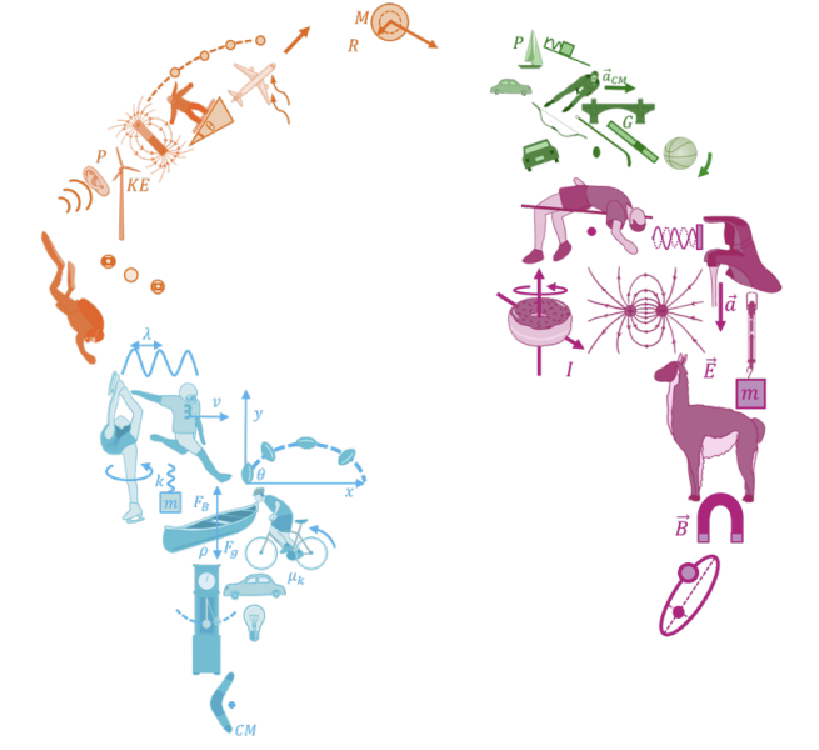
\includegraphics[width=4cm]{figures/BMDW/logo}
\end{textblock*}

\end{frame}

%%%%%%%%%%%%%TOC
\twocolframe{Outline}
  {\tableofcontents[sections={52,53}, subsectionstyle=show/show]\thispagestyle{empty}}
  {\tableofcontents[sections={54}, subsectionstyle=show/show]}
%%%%%%%%%%%%%%%%%%%%%%%%%







%%%%%%%%%%%%%%%%%%%%%%%%%%%%%%%%
\section{Electric Current}
\label{sec:electriccurrent}
\title{Electric Current}


%%%%%%%%%%%%%%%%%%%%%%%%%
\begin{frame}
\titlepage
\thispagestyle{empty}
\end{frame}

%%%%%%%%%%%%%%%%%%

\twocolframesf{Electric current}
{
\begin{itemize}
 \item Electric current is a measure of the rate at which charge flows through a material:
 \begin{align*}
 I = \frac{\Delta Q}{\Delta t}= \frac{dQ}{dt}
 \end{align*}
 \item Current is positive in the direction in which positive charges flow. In reality, it is \textbf{almost always electrons
that flow}, so current is usually in the \textit{opposite} direction of the flow of the actual charges.
 \item Electric current is a \textit{macroscopic} quantity. 
\end{itemize}
}
{
\centering
\begin{tikzpicture}[scale=0.5]
  \def\L{7.0}
  \def\h{3.0}
  \def\w{3.0}
  \def\H{4.0}
  
  %Electric field lines
  \begin{scope}[ decoration={
    markings,
    mark=at position 0.5 with {\arrow{latex}}}
    ] 
    
  \foreach \i in {1,...,7}
  {
    \draw[-latex,postaction={decorate}] (0,1/8*\h,-1/8*\i*\w) -- (\L,1/8*\h,-1/8*\i*\w);
    \draw[-latex,postaction={decorate}] (0,7/8*\h,-1/8*\i*\w) -- (\L,7/8*\h,-1/8*\i*\w);
  }

  \end{scope}
  
  %Current with arrow, first since needs to be "inside"
  \draw[line width=2pt,black, -latex,color=myred] (\L/4,\h/2,-\w/2) node[left] {$I$}  -- (\L/2,\h/2,-\w/2);  
  %Terminals: (The one on the left needs to be partially hidden)
  \draw[line width=3pt] (0, \h/2,-\w/2) --(0,\H+ \h/2,-\w/2) ;
  \draw[fill=black] (0,\H+ \h/2,-\w/2) circle (0.3)node[above=3pt] {$V_A$} node[left=2pt]{$+$};
  \draw[fill=black] (\L,\H+ \h/2,-\w/2) circle (0.3) node[above=3pt] {$V_B$}node[right=2pt]{$-$};
  \draw[line width=1pt,latex-latex] (\L/10,\H+ \h/2,-\w/2) -- (9*\L/10,\H+ \h/2,-\w/2) node[midway,above]{$\Delta V$};
  
  %Rectangle:
  \fill[left color=gray!30!,right color=gray!80,shading=axis,opacity=0.6, draw=black] (0,\h,0) -- (0,\h,-\w)--(\L,\h,-\w) -- (\L,\h,0);
  \fill[color=gray!90,opacity=0.6, draw=black] (\L,0,0) -- (\L,\h,0)--(\L,\h,-\w) -- (\L,0,-\w);
  %plane (inside)
  \fill[color=gray!20!black,opacity=0.5] (\L/2,0,0) -- (\L/2,\h,0)--(\L/2,\h,-\w) -- (\L/2,0,-\w);
  \draw[dashed] (0,\h,-\w) -- (0,0,-\w) -- (0,0,0);
  \draw[dashed] (0,0,-\w) -- (\L,0,-\w);
  %front face
  \fill[left color=gray!30!,right color=gray!80,shading=axis,opacity=0.4, draw=black] (0,0,0) -- (0,\h,0)--(\L,\h,0) -- (\L,0,0);
  %%%%%%%%%%% end of 3d rectangle

  %P

  \node[left] at (3/4*\L,\h/2,-\w/2) {$\vec E$} ;

  \draw[line width=3pt] (\L, \h/2,-\w/2) --(\L,\H+ \h/2,-\w/2) ;
  
 
  
\end{tikzpicture}
\captionof*{figure}{\textit{We apply a potential difference, $\Delta V$, across a metal and current, $I$, flows.}}

}



\def\proton at (#1,#2,#3){
\draw[fill=black,opacity=0.8] (#1,#2) circle (#3);
\node[text=white] at (#1,#2) {\tiny$+$};
\draw (#1+1.2*#3,#2) arc (0:90:1.2*#3);
\draw (#1+1.5*#3,#2) arc (0:90:1.5*#3);
\draw (#1+-1.2*#3,#2) arc (180:270:1.2*#3);
\draw (#1+-1.5*#3,#2) arc (180:270:1.5*#3);
}


%%%%%%%%%%%%%%%%%%%%%%%%%%%%%%
\subsection{Microscopic model of current}
\label{subsec:microscopicmodelofcurrent}
\twocolframesf{Microscopic model of current}
{
\begin{itemize}
 \item We can model current in a metal using a \textit{microscopic} model of charges ``drifting'' through the metal with an average velocity:
\begin{itemize}
 \item Typical \textbf{drift velocity}: $ v_d \sim \SI{1e-4}{m/s}$
 \end{itemize}
 \item In reality, electrons are moving around much faster, in mostly random directions and bouncing off of atoms:
\begin{itemize}
 \item Typical speed of electrons: \SI{1e8}{m/s}
 \end{itemize}
\end{itemize}
}
{
\centering

\begin{tikzpicture}[scale=0.5]
  \def\L{7.0}
  \def\R{2}
  \def\pr{0.25}
  
  %\proton at (0,3,0.25);

\proton at (0,0.7*\R,\pr);
\proton at (0,-0.7*\R,\pr);
\proton at (0,0,\pr);
\proton at (\L/10,0.35*\R,0.8*\pr);
\proton at (\L/10,-0.35*\R,0.8*\pr);
\proton at (0.2*\L,0,\pr);
\proton at (0.2*\L,0.7*\R,\pr);
\proton at (0.2*\L,-0.7*\R,\pr);
\proton at (0.3*\L,0.35*\R,1.2*\pr);
\proton at (0.3*\L,-0.35*\R,1.2*\pr);
\proton at (0.4*\L,0,\pr);
\proton at (0.4*\L,0.7*\R,\pr);
\proton at (0.4*\L,-0.7*\R,\pr);
\proton at (0.5*\L,0.35*\R,0.8*\pr);
\proton at (0.5*\L,-0.35*\R,0.8*\pr);
\proton at (0.6*\L,0,\pr);
\proton at (0.6*\L,0.7*\R,\pr);
\proton at (0.6*\L,-0.7*\R,\pr);
\proton at (0.7*\L,0.35*\R,1.2*\pr);
\proton at (0.7*\L,-0.35*\R,1.2*\pr);
\proton at (0.8*\L,0,\pr);
\proton at (0.8*\L,0.7*\R,\pr);
\proton at (0.8*\L,-0.7*\R,\pr);
\proton at (0.9*\L,0.35*\R,0.8*\pr);
\proton at (0.9*\L,-0.35*\R,0.8*\pr);
\proton at (\L,0,\pr);
\proton at (\L,0.7*\R,\pr);
\proton at (\L,-0.7*\R,\pr);

\draw[line width=1pt,-latex,color=myred] (\L,0) -- (\L-\L/10,\R/7) -- (\L-\L/6,-\R/2) --  (\L-\L/8,\R/2) -- (0.7*\L,0.2*\R) -- (0.5*\L,-0.8*\R)-- (0.45*\L,0.6*\R)-- (0.35*\L,-0.1*\R)-- (0.25*\L,0.3*\R)-- (0.15*\L,-0.3*\R)-- (0.,0.4*\R);
%cylinder:
  \fill[top color=gray!15!black,bottom color=gray!20,shading=axis,opacity=0.3, draw=black] (0,-\R) arc (270:90:\R/2 and \R) --  (0,\R)-- (\L, \R) arc (90:270:\R/2 and \R) -- (\L,-\R); 
  \draw[dashed] (0,\R) arc (90:-90:\R/2 and \R) ;
  \fill[color=gray!90,opacity=0.5,draw=black] (\L+\R/2, 0) arc (0:360:\R/2 and \R);
  %%%%%%%%%%
  %\draw[line width=1pt,latex-latex] (0,-1.1*\R) -- (\L,-1.1*\R) node[midway,below]{$\Delta V,L$};
  \draw[line width=3pt,-latex] (\L/4,1.2*\R) -- (3*\L/4,1.2*\R) node[midway,above]{$\vec E$};
  \draw[line width=1.5pt,color=myred,latex-] (0.4*\L,-1.1*\R) -- (0.6*\L,-1.1*\R) node[below, midway]{$\vec v_d$};
\end{tikzpicture}
\captionof*{figure}{\textit{An electron moving through a resistor and colliding with atoms, resulting in heat. The average speed of the electron is constant as the work done by the electric field is converted into heat.}}
}

%%%%%%%%%%%%%%%%%%%%%%%%%%%%%%
\def\electron at (#1,#2,#3){
\fill[color=myred,opacity=0.8] (#1,#2) circle (#3);
\draw[color=white] (#1-0.8*#3,#2) -- (#1+0.8*#3,#2); %- sign
\draw[color=myred,latex-] (#1-5*#3,#2) -- (#1-#3,#2);
}

\subsection{Drift velocity}
\label{subsec:driftvelocity}
\twocolframesf{Current and drift velocity}
{
We have, $n$, electrons per unit volume, with charge $q$, moving with average speed, $v_d$, through a resistor of cross-section, $A$: 
 \begin{itemize}
 \item<1-> In time $\Delta t$, electrons move a distance $l=v_d\Delta t$.
 \item<2-> This corresponds to a volume of electrons, $V=lA=v_d\Delta t A$
 \item<3-> with a total charge, $\Delta Q = Vnq = v_d\Delta t A nq$
 \item<4-> resulting in a current, $I$:\\
 $I=\frac{\Delta Q}{\Delta t}=v_d A nq$
 \end{itemize}
\only<5->{This allows us to relate a macroscopic quantity ($I$, current) to microscopic quantities (e.g. $v_d$).}
}
{
\centering

\begin{tikzpicture}[scale=0.5]
  \def\L{7.0}
  \def\R{2}
  \def\pr{0.15}
  
\electron at (0,0.7*\R,\pr);
\electron at (0,-0.7*\R,\pr);
\electron at (0,0,\pr);
\electron at (\L/10,0.35*\R,0.8*\pr);
\electron at (\L/10,-0.35*\R,0.8*\pr);
\electron at (0.2*\L,0,\pr);
\electron at (0.2*\L,0.7*\R,\pr);
\electron at (0.2*\L,-0.7*\R,\pr);
\electron at (0.3*\L,0.35*\R,1.2*\pr);
\electron at (0.3*\L,-0.35*\R,1.2*\pr);
\electron at (0.4*\L,0,\pr);
\electron at (0.4*\L,0.7*\R,\pr);
\electron at (0.4*\L,-0.7*\R,\pr);
\electron at (0.5*\L,0.35*\R,0.8*\pr);
\electron at (0.5*\L,-0.35*\R,0.8*\pr);
\electron at (0.6*\L,0,\pr);
\electron at (0.6*\L,0.7*\R,\pr);
\electron at (0.6*\L,-0.7*\R,\pr);
\electron at (0.7*\L,0.35*\R,1.2*\pr);
\electron at (0.7*\L,-0.35*\R,1.2*\pr);
\electron at (0.8*\L,0,\pr);
\electron at (0.8*\L,0.7*\R,\pr);
\electron at (0.8*\L,-0.7*\R,\pr);
\electron at (0.9*\L,0.35*\R,0.8*\pr);
\electron at (0.9*\L,-0.35*\R,0.8*\pr);
\electron at (\L,0,\pr);
\electron at (\L,0.7*\R,\pr);
\electron at (\L,-0.7*\R,\pr);

%cylinder:
  \fill[top color=gray!15!black,bottom color=gray!20,shading=axis,opacity=0.3, draw=black] (0,-\R) arc (270:90:\R/2 and \R) --  (0,\R)-- (\L, \R) arc (90:270:\R/2 and \R) -- (\L,-\R); 
  \draw[dashed] (0,\R) arc (90:-90:\R/2 and \R) ;
  \fill[color=gray!90,opacity=0.5,draw=black] (\L+\R/2, 0) arc (0:360:\R/2 and \R);
%%%%%%  
   \fill[left color=myred!30!,right color=myred!80,shading=axis,opacity=0.3, draw=myred] (3*\L/8,-\R) arc (270:90:\R/2 and \R) --  (3*\L/8,\R)-- (5*\L/8, \R) arc (90:270:\R/2 and \R) -- (5*\L/8,-\R); 
  \draw[dashed,color=myred] (3*\L/8,\R) arc (90:-90:\R/2 and \R) ;
  \fill[color=myred!90,opacity=0.3,draw=myred] (5*\L/8+\R/2, 0) arc (0:360:\R/2 and \R);  
%%%%%%%%%%%%%%55 
  \node at (1.2*\L,0) {$A$};
  \draw[line width=1pt,latex-latex] (3*\L/8,-1.1*\R) -- (5*\L/8,-1.1*\R) node[midway,below]{$l=v_d\Delta t$};
  \draw[line width=3pt,-latex] (\L/4,1.2*\R) -- (3*\L/4,1.2*\R) node[midway,above]{$\vec E$};
\end{tikzpicture}
\captionof*{figure}{\textit{Electrons drifting with an average velocity, $\vec v_d$}}
}

%%%%%%%%%%%%%%%%%%%%%%%%%%%%%%
\twocolframesf{Current and current density}
{
\begin{itemize}
 \item We can model charges moving through a metal macroscopically, by using current, $I$:
\begin{align*}
I = \frac{dQ}{dt}
\end{align*}
This is the amount of charge flowing through cross section, $A$, of the metal per unit time.
 \item We can define the current density, as the current per unit area, $j$:
\begin{align*}
j = \frac{I}{A}
\end{align*}
$j$, the current density can depend on position and is a microscopic quantity.
\end{itemize}

}
{
\centering

\begin{tikzpicture}[scale=0.5]
  \def\L{7.0}
  \def\R{2}
  \def\pr{0.15}
  
%cylinder:
  \fill[top color=gray!15!black,bottom color=gray!20,shading=axis,opacity=0.3, draw=black] (0,-\R) arc (270:90:\R/2 and \R) --  (0,\R)-- (\L, \R) arc (90:270:\R/2 and \R) -- (\L,-\R); 
  \draw[dashed] (0,\R) arc (90:-90:\R/2 and \R) ;
  \fill[color=gray!90,opacity=0.5,draw=black] (\L+\R/2, 0) arc (0:360:\R/2 and \R);
%%%%%%  
 
  \node at (1.2*\L,0) {$A$};

  \draw[line width=3pt,-latex] (\L/4,1.2*\R) -- (3*\L/4,1.2*\R) node[midway,above]{$\vec E$};
  \draw[line width=1.5pt,color=myred,-latex] (0.35*\L,0) -- (0.65*\L,0) node[above, midway]{$\vec j$};
\end{tikzpicture}
\captionof*{figure}{\textit{Current density is a vector parallel to the electric field (and anti-parallel to drift velocity for electrons).}}
}

%%%%%%%%%%%%%%%%%%%%%%%%%%%%%%
\subsection{Current density}
\label{subsec:currentdensity}
\subsubsection{At the microscopic level}
\label{subsubsec:atthemicroscopiclevel}
\twocolframesf{Current density at the microscopic level}
{
\begin{itemize}
 \item We define the \textbf{current density, $\vec j$, as a vector parallel to the electric field}, corresponding to the direction of the average flow of positive charges.
\item If we choose a surface, the current through that surface is that part of the current density flowing perpendicular to the surface:
\begin{align*}
I = \int \vec j \cdot d\vec A=\int j dA_\perp
\end{align*}
(just like a ``flux''; in fact, exactly a flux!)
\end{itemize}
}
{
\centering

\begin{tikzpicture}[scale=0.5]
  \def\L{7.0}
  \def\R{2}
  \def\pr{0.15}
  
  \begin{scope}[xshift=2.5cm, rotate=-30]
  \fill[color=gray!80,draw=black] (0.,0) ellipse(0.15*\R/1 and 0.3*\R);
  \draw[line width=1.5pt,color=black,-latex] (0,0) -- (0.2*\L,0) node[right]{$d\vec A$};
  \end{scope}
  
%cylinder:
  \fill[top color=gray!15!black,bottom color=gray!20,shading=axis,opacity=0.3, draw=black] (0,-\R) arc (270:90:\R/2 and \R) --  (0,\R)-- (\L, \R) arc (90:270:\R/2 and \R) -- (\L,-\R); 
  \draw[dashed] (0,\R) arc (90:-90:\R/2 and \R) ;
  \fill[color=gray!90!,opacity=0.5,draw=black] (\L+\R/2, 0) arc (0:360:\R/2 and \R);
%%%%%%  
 
  \node at (1.2*\L,0) {$A$};

  \draw[line width=3pt,-latex] (\L/4,1.2*\R) -- (3*\L/4,1.2*\R) node[midway,above]{$\vec E$};
  \draw[line width=1.5pt,color=myred,-latex] (0.35*\L,0) -- (0.65*\L,0) node[above, midway]{$\vec j$};
\end{tikzpicture}
\captionof*{figure}{\textit{Current density is a vector parallel to the electric field (and anti-parallel to drift velocity for electrons).}}
}


%%%%%%%%%%%%%%%%%%%%%%%%%%%%%%
\subsubsection{From drift velocity}
\label{subsubsec:fromdriftvelocity}
\begin{bulletframe}{Current density from drift velocity}
\item The current:
\begin{align*}
\vec I = -enA\vec v_d
\end{align*}
\item The current density:
\begin{align*}
\vec j= \frac{\vec I}{A} = -en\vec v_d
\end{align*}
Here, we have explicitly chosen negative charges (electrons with charge $q=-e=\SI{-1.6e-19}{C}$). Current and current density are in the opposite direction of the drift velocity because $q$ is negative.
\end{bulletframe}

%%%%%%%%%%%%%%%%%%%%%%%%%%%%%%





\section{Ohm's Law}
\label{sec:ohmslaw}
\title{Ohm's Law}


%%%%%%%%%%%%%%%%%%%%%%%%%
\begin{frame}
\titlepage
\thispagestyle{empty}
\end{frame}





%%%%%%%%%%%%%%%%%%%%%%%%%%%%
\begin{bulletframe}{Ohm's Law}
\item For most materials:
\begin{align*}
\vec j= \sigma \vec E
\end{align*}
(We call these ``ohmic'' materials, because the law holds).
\item $\sigma$ is the \textbf{conductivity} of the material; it is a material-dependent measure of how large a current density one gets for a given applied electric field.
\end{bulletframe}


%%%%%%%%%%%%%%%%%%%%%%%%%%%%%%
\subsection{Macroscopically}
\label{subsec:macroscopically}
\twocolframesf{Ohm's Law, macroscopically}
{
\begin{itemize}
\item Microscopically:
\begin{align*}
\vec j= \frac{\vec I}{A} = -en\vec v_d\;\;\;\;\vec j = \sigma\vec E
\end{align*}
\item Relation between current and current density, on a \textit{macroscopic} piece of metal: 
\begin{align*}
\frac{I}{A} &= \sigma E=\sigma \frac{\Delta V}{L}\\
\only<1>{
\therefore \Delta V &= \frac{1}{\sigma}\frac{L}{A}I\\
}
\only<2>{
\therefore \Delta V &= \textcolor{myred}{\frac{1}{\sigma}\frac{L}{A}}I\\
\Aboxed{\Delta V &=\textcolor{myred}{R} I}
}
\end{align*}
\end{itemize}
}
{
\only<1>{
\centering
\begin{tikzpicture}[scale=0.5]
  \def\L{7.0}
  \def\h{3.0}
  \def\w{3.0}
  \def\H{4.0}
  
  %Electric field lines
  \begin{scope}[ decoration={
    markings,
    mark=at position 0.5 with {\arrow{latex}}}
    ] 
    
  \foreach \i in {1,...,7}
  {
    \draw[-latex,postaction={decorate}] (0,1/8*\h,-1/8*\i*\w) -- (\L,1/8*\h,-1/8*\i*\w);
    \draw[-latex,postaction={decorate}] (0,7/8*\h,-1/8*\i*\w) -- (\L,7/8*\h,-1/8*\i*\w);
  }

  \end{scope}
  
  %Current with arrow, first since needs to be "inside"
  \draw[line width=2pt,black, -latex,color=myred] (\L/4,\h/2,-\w/2) node[left] {$I$}  -- (\L/2,\h/2,-\w/2);  
  %Terminals: (The one on the left needs to be partially hidden)
  \draw[line width=3pt] (0, \h/2,-\w/2) --(0,\H+ \h/2,-\w/2) ;
  \draw[fill=black] (0,\H+ \h/2,-\w/2) circle (0.3)node[above=3pt] {$V_A$} node[left=2pt]{$+$};
  \draw[fill=black] (\L,\H+ \h/2,-\w/2) circle (0.3) node[above=3pt] {$V_B$}node[right=2pt]{$-$};
  \draw[line width=1pt,latex-latex] (\L/10,\H+ \h/2,-\w/2) -- (9*\L/10,\H+ \h/2,-\w/2) node[midway,above]{$\Delta V=EL$};
  
  %Rectangle:
  \fill[left color=gray!30!,right color=gray!80,shading=axis,opacity=0.6, draw=black] (0,\h,0) -- (0,\h,-\w)--(\L,\h,-\w) -- (\L,\h,0);
  \fill[color=gray!90,opacity=0.6, draw=black] (\L,0,0) -- (\L,\h,0)--(\L,\h,-\w) -- (\L,0,-\w);
  %plane (inside)
  \fill[color=gray!20!black,opacity=0.5] (\L/2,0,0) -- (\L/2,\h,0)--(\L/2,\h,-\w) -- (\L/2,0,-\w);
  \draw[dashed] (0,\h,-\w) -- (0,0,-\w) -- (0,0,0);
  \draw[dashed] (0,0,-\w) -- (\L,0,-\w);
  %front face
  \fill[left color=gray!30!,right color=gray!80,shading=axis,opacity=0.4, draw=black] (0,0,0) -- (0,\h,0)--(\L,\h,0) -- (\L,0,0);
  %%%%%%%%%%% end of 3d rectangle

  %Some labels
  \node[left] at (3/4*\L,\h/2,-\w/2) {$\vec E$} ;
  \draw[line width=3pt] (\L, \h/2,-\w/2) --(\L,\H+ \h/2,-\w/2) ;
  \draw[line width=1pt,latex-latex] (0,-\h/10,0) -- (\L,-\h/10,0) node[midway,below]{$L$};
  \node[left] at (1.25*\L,\h/2,-\w/2) {$A$} ;
  
\end{tikzpicture}
\captionof*{figure}{\textit{We apply a potential difference, $\Delta V$, across a metal and current, $I$, flows due to the electric field, $\vec E$.}}
}
\only<2>{
\begin{block}{Resistance}

We call, $R$, the ``resistance'' of the piece of material (a ``resistor''). 
\begin{align*}
R=\frac{1}{\sigma}\frac{L}{A}=\rho\frac{L}{A}
\end{align*}
where $\rho$ is the ``resistivity'' and $\sigma$ the ``conductivity'' of the material.\\
\textbf{Resistance} is the macroscopic property of resistor of length, $L$, area, $A$, made from a material with resistivity, $\rho$.
\end{block}
}

}


%%%%%%%%%%%%%%%%%%%%%%%%%%%%%%





%%%%%%%%%%%%%%%%%%%%%%%
\twocolframesf{Ohm's Law}
{
%\vspace{-1.5cm}
\begin{itemize}
\item Technically, Ohm’s Law refers to the microscopic version, $\vec j=\sigma \vec E$.
\item Ohm noted that the current through a material is proportional to the electric potential difference, introducing ``resistance'', $R$, as the constant of proportionality:
\begin{align*}
\Delta V \propto I= R I
\end{align*}
\item  For any ``resistor'' can use Ohm’s Law to find the current through it, given a potential difference.
\item High resistance $=$ low current for a given electric field
\end{itemize}


}
{
}

%%%%%%%%%%%%%%%%%%%%%%%%%%%%%%






%%%%%%%%%%%%%%%%%%%%%%%%%%%%%%5

\subsection{Resistance}
\label{subsec:resistance}
\twocolframesf{Resistance}
{
\begin{itemize}
\item Ohm's law for a resistor:
\begin{align*}
\Delta V = R I
\end{align*}
\item The resistance depends on the shape, $(L,A)$, and the material, $\rho$:
\begin{align*}
R=\rho\frac{L}{A}
\end{align*}
\only<2>{
\item Recall Poiseuille flow (fluid with viscosity):
\begin{align*}
\Delta P = R Q
\end{align*}
\item For a horizontal pipe: $R=\frac{8\eta L}{\pi r^4}$
}
\end{itemize}

}
{
\centering
\only<1>{
\begin{tikzpicture}[scale=0.5]
  \def\L{7.0}
  \def\h{3.0}
  \def\w{3.0}
  \def\H{4.0}
  
  %Electric field lines
  \begin{scope}[ decoration={
    markings,
    mark=at position 0.5 with {\arrow{latex}}}
    ] 
    
  \foreach \i in {1,...,7}
  {
    \draw[-latex,postaction={decorate}] (0,1/8*\h,-1/8*\i*\w) -- (\L,1/8*\h,-1/8*\i*\w);
    \draw[-latex,postaction={decorate}] (0,7/8*\h,-1/8*\i*\w) -- (\L,7/8*\h,-1/8*\i*\w);
  }

  \end{scope}
  
  %Current with arrow, first since needs to be "inside"
  \draw[line width=2pt,black, -latex,color=myred] (\L/4,\h/2,-\w/2) node[left] {$I$}  -- (\L/2,\h/2,-\w/2);  
  %Terminals: (The one on the left needs to be partially hidden)
  \draw[line width=3pt] (0, \h/2,-\w/2) --(0,\H+ \h/2,-\w/2) ;
  \draw[fill=black] (0,\H+ \h/2,-\w/2) circle (0.3)node[above=3pt] {$V_A$} node[left=2pt]{$+$};
  \draw[fill=black] (\L,\H+ \h/2,-\w/2) circle (0.3) node[above=3pt] {$V_B$}node[right=2pt]{$-$};
  \draw[line width=1pt,latex-latex] (\L/10,\H+ \h/2,-\w/2) -- (9*\L/10,\H+ \h/2,-\w/2) node[midway,above]{$\Delta V=RI$};
  
  %Rectangle:
  \fill[left color=gray!30!,right color=gray!80,shading=axis,opacity=0.6, draw=black] (0,\h,0) -- (0,\h,-\w)--(\L,\h,-\w) -- (\L,\h,0);
  \fill[color=gray!90,opacity=0.6, draw=black] (\L,0,0) -- (\L,\h,0)--(\L,\h,-\w) -- (\L,0,-\w);
  %plane (inside)
  \fill[color=gray!20!black,opacity=0.5] (\L/2,0,0) -- (\L/2,\h,0)--(\L/2,\h,-\w) -- (\L/2,0,-\w);
  \draw[dashed] (0,\h,-\w) -- (0,0,-\w) -- (0,0,0);
  \draw[dashed] (0,0,-\w) -- (\L,0,-\w);
  %front face
  \fill[left color=gray!30!,right color=gray!80,shading=axis,opacity=0.4, draw=black] (0,0,0) -- (0,\h,0)--(\L,\h,0) -- (\L,0,0);
  %%%%%%%%%%% end of 3d rectangle

  %Some labels
  \node[left] at (3/4*\L,\h/2,-\w/2) {$\vec E$} ;
  \draw[line width=3pt] (\L, \h/2,-\w/2) --(\L,\H+ \h/2,-\w/2) ;
  \draw[line width=1pt,latex-latex] (0,-\h/10,0) -- (\L,-\h/10,0) node[midway,below]{$L$};
  \node[left] at (1.25*\L,\h/2,-\w/2) {$A$} ;
  
\end{tikzpicture}
\captionof*{figure}{\textit{We apply a potential difference, $\Delta V$, across a resistor, $R$, and current, $I$, flows.}}
}

\only<2>{
\begin{tikzpicture}[scale=0.5]
  \def\L{7.0}
  \def\R{2}
  \def\pr{0.15}
  
  \draw[line width=1.5pt,color=myred,-latex] (0.35*\L,0) -- (0.65*\L,0) node[above, midway]{$Q$};
    
%cylinder:
  \fill[top color=myblue!85,bottom color=myblue!20,shading=axis,opacity=0.4, draw=black] (0,-\R) arc (270:90:\R/2 and \R) --  (0,\R)-- (\L, \R) arc (90:270:\R/2 and \R) -- (\L,-\R); 
  \draw[dashed] (0,\R) arc (90:-90:\R/2 and \R) ;
  \fill[color=myblue!90,opacity=0.6,draw=black] (\L+\R/2, 0) arc (0:360:\R/2 and \R);
%%%%%%  
 
  \node at (1.2*\L,0) {$A$};
  \draw[line width=1pt,latex-latex] (0,1.1*\R) -- (\L,1.1*\R) node[midway,above]{$\Delta P$};

\end{tikzpicture}
\captionof*{figure}{\textit{A fluid flowing through a pipe due to a pressure difference.}}
\begin{exampleblock}{Analogy}
The math for current flowing through a resistor is the same as for fluid flowing through a pipe! Voltage is like pressure difference. 
\end{exampleblock}
}
}



%%%%%%%%%%%%%%%%%%%%%%%%%%%%%%




%%%%%%%%%%%%%%%%%%%%%%%%%%%%%%
\subsection{Combining resistors}
\label{subsec:combiningresistors}
\twocolframe{Combining resistors}
{
\only<1>{
\textbf{In series:} The voltages across each resistor add up to the battery voltage:
 \begin{align*}
 \Delta V_1 + \Delta V_2 &=\Delta V\\
  R_1I+R_2I&=R_{eff}I
 \end{align*}
Like making a longer resistor, total resistance increases:
\begin{align*}
R_{eff}=R_1+R_2
\end{align*} 
}
\only<2>{
\textbf{In parallel:} The currents through each resistor add up to the current through the battery:
 \begin{align*}
 I_1+I_2&= I\\
 \frac{\Delta V}{R_1}+\frac{\Delta V}{R_1}&= \frac{\Delta V}{R_{eff}}
 \end{align*}

Like making a wider resistor, total resistance decreases:
\begin{align*}
\frac{1}{R_{eff}}=\frac{1}{R_1}+\frac{1}{R_2}
\end{align*}
}
}
{
\begin{center}
\begin{tikzpicture}
\tikzmath{
\L=6;
\Lh=0.75;
\termh=0.25;
\h=1.5;
\Rh=0.75;
\Rl=0.35*\L;
\wl=(\L-3*\termh-2*\Rl)/3;
\wlp=(\L-3*\termh-\Rl)/2;
}
\scalebox{1}{
%battery and terminals:
\coordinate (T1) at (1.5*\termh,\termh);
\coordinate (T2) at (\L-1.5*\termh,\termh);

\fill[color=myblue!30,rounded corners] (0,-\Lh) rectangle (\L,0);
\fill[color=myblue!60] (\termh,0) rectangle +(\termh,\termh);
\fill[color=myblue!60] (\L-\termh,0) rectangle +(-\termh,\termh);
\node[below] at ($(T1)+((0,-\termh)$){$+$};
\node[below] at ($(T2)+((0,-\termh)$){$-$};
\draw[latex-latex] ($(T1)+(0,0.1)$) -- ($(T2)+(0,0.1)$) node[midway,above]{$\Delta V$};

%wires and resistors
\only<1>{
\draw[line width = 2] (T1) -- ($(T1)+(0,\h)$) -- ($(T1)+(\wl,\h)$);
\fill[color=myblue!30,rounded corners] ($(T1)+(\wl,\h-0.5*\Rh)$) rectangle +(\Rl,\Rh);
\draw[line width = 2] ($(T1)+(\wl+\Rl,\h)$) -- +(\wl,0);
\fill[color=myblue!30,rounded corners] ($(T1)+(2*\wl+\Rl,\h-0.5*\Rh)$) rectangle +(\Rl,\Rh);
\draw[line width = 2] ($(T1)+(2*\wl+2*\Rl,\h)$) -- +(\wl,0) -- (T2);

\node at ($(T1)+(\wl+\Rl/2,\h)$){$R_1$};
\node at ($(T1)+(2*\wl+1.5*\Rl,\h)$){$R_2$};

\draw[latex-latex] ($(T1)+(\wl,\h+0.5*\Rh+0.1)$) -- +(\Rl,0) node[midway,above]{$\Delta V_1=R_1I$};
\draw[latex-latex] ($(T1)+(2*\wl+\Rl,\h+0.5*\Rh+0.1)$) -- +(\Rl,0) node[midway,above]{$\Delta V_2=R_2I$};

\draw[-latex,line width=2, color=myred] ($(T1)+(0,0.4*\h)$) -- +(0,0.2*\h) node[left]{$I$};
\draw[-latex,line width=2, color=myred] ($(T2)+(0,0.6*\h)$) -- +(0,-0.2*\h) node[right]{$I$}; 
\draw[-latex,line width=2, color=myred] ($(T1)+(\wl+\Rl,\h)$) -- +(1.2*\wl,0) node[midway,below]{$I$};

\draw[dotted,line width=2, color=myblue!80] ($(T1)+(0.5*\wl,0.5*\h)$) rectangle +(2*\Rl+2*\wl,1.3*\h);
\node[above=5pt, color=myblue!80] at (0.5*\L,1.8*\h){$R_{eff}$};
}

\only<2>{
\draw[line width = 2] (T1) -- ($(T1)+(0,\h)$) -- ($(T1)+(\wlp,\h)$);
\fill[color=myblue!30,rounded corners] ($(T1)+(\wlp,\h-0.5*\Rh)$) rectangle +(\Rl,\Rh);
\draw[line width = 2] ($(T1)+(\wlp+\Rl,\h)$) -- +(\wlp,0) -- (T2);
\node at (\L/2,\termh+\h){$R_1$};
\draw[latex-latex] ($(T1)+(\wlp,\h+0.5*\Rh+0.1)$) -- +(\Rl,0) node[midway,above]{$\Delta V_1=R_1I_1$};


\draw[line width = 2] (T1) -- ($(T1)+(0,2*\h)$) -- ($(T1)+(\wlp,2*\h)$);
\fill[color=myblue!30,rounded corners] ($(T1)+(\wlp,2*\h-0.5*\Rh)$) rectangle +(\Rl,\Rh);
\draw[line width = 2] ($(T1)+(\wlp+\Rl,2*\h)$) -- +(\wlp,0) -- (T2);
\node at (\L/2,\termh+2*\h){$R_2$};
\draw[latex-latex] ($(T1)+(\wlp,2*\h+0.5*\Rh+0.1)$) -- +(\Rl,0) node[midway,above]{$\Delta V_2=R_2I_2$};

\draw[-latex,line width=2, color=myred] ($(T1)+(0,0.4*\h)$) -- +(0,0.2*\h) node[left]{$I$};
\draw[-latex,line width=2, color=myred] ($(T2)+(0,0.6*\h)$) -- +(0,-0.2*\h) node[right]{$I$}; 

\draw[-latex,line width=2, color=myred] ($(T1)+(0.4*\wlp,\h)$) -- +(0.2*\wlp,0) node[below]{$I_1$};
\draw[-latex,line width=2, color=myred] ($(T1)+(0.4*\wlp,2*\h)$) -- +(0.2*\wlp,0) node[below]{$I_2$};
\draw[-latex,line width=2, color=myred] ($(T1)+(1.4*\wlp+\Rl,\h)$) -- +(0.2*\wlp,0) node[below]{$I_1$};
\draw[-latex,line width=2, color=myred] ($(T1)+(1.4*\wlp+\Rl,2*\h)$) -- +(0.2*\wlp,0) node[below]{$I_2$};

\draw[dotted,line width=2, color=myblue!80] ($(T1)+(0.75*\wlp,0.5*\h)$) rectangle +(\Rl+0.5*\wlp,2.3*\h);
\node[above=5pt, color=myblue!80] at (0.5*\L,2.8*\h){$R_{eff}$};


}

}
\end{tikzpicture}
\captionof*{figure}{\textit{\only<1>{$R_1$ and $R_2$ in series.}\only<2>{$R_1$ and $R_2$ in parallel.}}}
\end{center}
}




%%%%%%%%%%%%%%%%%%%%%%%%%%%%%%
\subsection{Resistivity}
\label{subsec:resistivity}
\begin{bulletframe}{Resistivity}
\item Resistivity is a temperature-dependent property of a material:
\begin{align*}
R = \rho(T)\frac{L}{A}
\end{align*}
\item The temperature dependence, is ``often'' linear (for most materials, for common ranges of temperatures):
\begin{align*}
\rho(T) = \rho_0\left[1+\alpha(T-T_0)\right]
\end{align*}
\item We use a reference resistivity, $\rho_0$, at a reference temperature, $T_0$, (usually $T_0=\SI{20}{\degree C}$).
\item Note that $\alpha$, the temperature coefficient, depends on the choice of reference temperature, $T_0$.
\end{bulletframe}


%%%%%%%%%%%%%%%%%%%%%%%%%%%%%%
\subsubsection{Resistivity versus temperature}
\label{subsubsec:resistivityversustemperature}
\twocolframesf{Resistivity versus temperature}
{
\begin{itemize}
\item The resistivity is linear in temperature:
\begin{align*}
\rho(T) = \rho_0\left[1+\alpha(T-T_0)\right]
\end{align*}
\item Remember, conductors resist the flow of current, because there are atoms in the conductor that the
charges run into.
\item If those atoms are shaking around more, it’s more likely for the flowing charges to run into them.
\begin{itemize}
\item More shaking $\rightarrow$ higher temperature.
\item More running into atoms $\rightarrow$ higher resistance.
\end{itemize}
\end{itemize}
}
{
\centering
\begin{tikzpicture}[scale=0.4]
  \def\ro{6.0}
  \def\To{6.0}
  \def\alp{1.}
  
  \draw[-latex](0,0)--(10,0) node[below] {$T$};
  \draw[-latex](0,0)--(0,10) node[left] {$\rho$};
  \draw[color=red, line width=2pt] (0,3)--(9,7.5);
  \fill (6,6) circle(5pt);
  \fill (0,3) circle(5pt);
  \node[below=3pt, right] at (0,3) {$\rho_0-\rho_0\alpha T_0$} ;
  \draw[dotted,line width=1.5pt] (0,\ro) -- (\To,\ro);
  \node[left] at (0,\ro) {$\rho_0$} ;
  \draw[dotted,line width=1.5pt] (\To,\ro) -- (\To,0);
  \node[below] at (\To,0) {$T_0$} ;
  
\end{tikzpicture}
\captionof*{figure}{\textit{Resistivity as a function of temperature. It's a silly parametrization, because the slope is $\rho_0 \alpha$ instead of just $\alpha$.}}
}


%%%%%%%%%%%%%%%%%%%%%%%%%%%%%%
\subsubsection{Resistivity for a few materials}
\label{subsubsec:resistivityforafewmaterials}
\begin{frame}{Resistivity for a few materials}
\capfig{1}{figures/Current/table}{}

\end{frame}


%%%%%%%%%%%%%%%%%%%%%%%%%%%%%%
\subsection{Measuring resistance}
\label{subsec:measuringresistance}
\twocolframesf{Measuring resistance}
{
\begin{itemize}
\item Instead of a battery, we use a constant current source
\item We can measure the voltage across the resistor to find its resistance:
\begin{align*}
\Delta V = RI
\end{align*}
\item What is the resistance at room temperature ?
\end{itemize}
}
{
\begin{circuitikz}[]
\draw (0,0) [short] to (0,2)
      to [R,l_=$R$,i>=$I$] (4,2) 
      to [short,i>=$I$] (4,0) 
      to [current source,l^=$I$](0,0);  
\draw (1,2) [short,-*] to (1,3);
\draw (3,2) [short,-*] to (3,3);
\draw (1,3) [voltmeter] to (3,3);
\end{circuitikz}
\captionof*{figure}{\textit{Constant current source connected to a resistor. A voltmeter measures the voltage, $\Delta V$, across the resistor.}}
}



%%%%%%%%%%%%%%%%%%%%%%%%%%%%%%




%%%%%%%%%%%%%%%%%%%%%%%%%%%%%%
\subsection{Resistance versus temperature}
\label{subsec:resistanceversustemperature}
\twocolframesf{Resistance versus temperature}
{
What is the resistance
\begin{itemize}
\item At \SI{20}{\degree C} (room temperature)?
\item At \SI{0}{\degree C} (ice water)?
\item At \SI{100}{\degree C} (boiling water)?
\item At \SI{-196}{\degree C} (liquid nitrogen)?
\end{itemize}
}
{
\begin{circuitikz}[]
\draw (0,0) [short] to (0,2)
      to [R,l_=$R$,i>=$I$] (4,2) 
      to [short,i>=$I$] (4,0) 
      to [current source,l^=$I$](0,0);  
\draw (1,2) [short,-*] to (1,3);
\draw (3,2) [short,-*] to (3,3);
\draw (1,3) [voltmeter] to (3,3);
\end{circuitikz}
\captionof*{figure}{\textit{Constant current source connected to a resistor. A voltmeter measures the voltage, $\Delta V$, across the resistor.}}
}


%%%%%%%%%%%%%%%%%%%%%%%%%%%%%%



%%%%%%%%%%%%%%%%%%%%%%%%%%%%%%
\twocolframesf{Resistance versus temperature}
{
What is the resistance
\begin{itemize}
\item At \SI{-196}{\degree C} (liquid nitrogen)? \SI{1.32}{\Omega}
\item At \SI{0}{\degree C} (ice water)? \SI{6.0}{\Omega}
\item At \SI{20}{\degree C} (room temperature)? \SI{7.0}{\Omega}
\item At \SI{100}{\degree C} (boiling water)? \SI{8.0}{\Omega}
\end{itemize}
\begin{align*}
 R(T) &= R_0 \left[1+\alpha(T-T_0)\right]
\end{align*}
To get $\alpha$:
\begin{itemize}
\item Fit the data (the slope is $\alpha R_0$). Better method since it uses all the data.
\item Use the equation above at a given value of $T$.7
\end{itemize}
}
{
\capfig{1}{figures/Current/plot}{The resistivity is linear over \SI{300}{\degree C}!}

}

%%%%%%%%%%%%%%%%%%%%%%%%%%%%%%%%%



%%%%%%%%%%%%%%%%%%%%%%%%%%%%%%%%%%%%%%


\begin{frame}{Resistance vs Temperature}

\capfig{0.55}{figures/Current/RvsT}{Data from the previous lecture. Resistance is linear from \SI{-196}{\celsius} to \SI{100}{\celsius}!}

\end{frame}


%%%%%%%%%%%%%%%%%%%%%%%%%%%%%%







\section{Electrical Power}
\label{sec:electricalpower}
\title{Electrical Power}


%%%%%%%%%%%%%%%%%%%%%%%%%
\begin{frame}
\titlepage
\thispagestyle{empty}
\end{frame}




%%%%%%%%%%%%%%%%%%%%%%%%%%%%%%
\subsection{Batteries}
\label{subsec:batteries}
\twocolframesf{Batteries}
{
\begin{itemize}
\item Batteries have a positive ($+$) terminal and a negative terminal ($-$).
\item Batteries are characterized by the difference in electric potential between the positive and negative terminal that
they provide, e.g. a $\SI{9}{V}$ battery.
\item Most batteries exploit the properties of different materials to create an electrical potential difference.
\begin{itemize}
\item Often, this is done by exploiting the different affinities for materials to be dissolved in acid.
\end{itemize}
\end{itemize}
}
{
}

%%%%%%%%%%%%%%%%%%%%%%%%%%%%%%
%%%%%%%%%%%%% Defs for next figure
\def\proton at (#1,#2,#3){
\draw[fill=black,opacity=1] (#1,#2) circle (#3);
% a plus sign that scales
\draw[color=white] (#1-0.8*#3,#2) -- (#1+0.8*#3,#2);
\draw[color=white] (#1,#2-0.8*#3) -- (#1,#2+0.8*#3);
}

\def\ion at (#1,#2,#3){
\draw[fill=orange,opacity=1,draw=orange] (#1,#2) circle (#3);
% a plus sign that scales
\draw[color=white] (#1-0.8*#3,#2) -- (#1+0.8*#3,#2);
\draw[color=white] (#1,#2-0.8*#3) -- (#1,#2+0.8*#3);
}

\def\electron at (#1,#2,#3){
\fill[color=myred,opacity=1] (#1,#2) circle (#3);
% a minus sign that scales
\draw[color=white] (#1-0.8*#3,#2) -- (#1+0.8*#3,#2);
}

\subsection{The electric cell}
\label{subsec:theelectriccell}
\twocolframe{The electric cell}
{
\begin{itemize}
\item Zinc ``likes'' to be dissolved as an ion in acid.
\item The zinc ions leave their electrons behind in the electrode, making the zinc electrode negatively charged.
\item Electrons that are loosely bound in a carbon electrode are attracted into the electrolyte solution, leaving the carbon electrode positively charged.
\item Very quickly, the process stops as an equilibrium is reached, with a net electric potential difference between electrodes.
\end{itemize}
}
{ 
\begin{center}

\begin{tikzpicture}[scale=1]
\tikzmath{
\Lou=2.0;
\Lw=1.0;
\Rou=1.5;
\dr=0.07;
\fac=0.3;
\Rd=0.17;
\Ld=3.3;
\xs=0.7;
\rp=0.1;
\re=0.05;
}  

\scalebox{1}{
%liquid:
  \fill[color=myblue!80,opacity=0.5] (-\Rou,0) arc (180:360:{\Rou} and {\fac*\Rou}) --  (\Rou,0)-- (\Rou, \Lw) arc (0:-180:{\Rou} and {\fac*\Rou}) -- (-\Rou,\Lw); 
  \fill[color=myblue!60, opacity=0.5] (\Rou,\Lw) arc (0:360:{\Rou} and {\fac*\Rou}) ;
 \draw[color=black] (\Rou,\Lw) arc (0:180:{\Rou} and {\fac*\Rou}) ;

%BACK RIM OF CONTAINER
  \draw[color=myblue!50, color=black, opacity=1, name path=A1] (\Rou,\Lou) arc (0:180:{\Rou} and {\fac*\Rou}) ;
  \draw[color=myblue!20, color=black, opacity=1, name path=B1] (\Rou-\dr,\Lou) arc (0:180:{\Rou-\dr} and {\fac*(\Rou-\dr)});
  \tikzfillbetween[of=A1 and B1]{gray}; 
  
%Rods:
  \fill[color=black!70,opacity=0.9] (-\Rd-\xs,0) arc (180:360:{\Rd} and {\fac*\Rd}) --  (\Rd-\xs,0)-- (\Rd-\xs, \Ld) arc (0:-180:{\Rd} and {\fac*\Rd}) -- (-\Rd-\xs,\Ld); 
  \fill[color=black!70, opacity=0.9] (\Rd-\xs,\Ld) arc (0:360:{\Rd} and {\fac*\Rd}) ;
  %\draw[color=black, dashed] (\Rd-\xs,\Lw) arc (0:360:{\Rd} and {\fac*\Rd}) ;
  \fill[color=myblue!50, opacity=0.5] (\Rd-\xs,\Lw) arc (0:-180:{\Rd} and {\fac*\Rd})  -- (-\xs-\Rd,\Lw-0.95) -- (-\xs+\Rd,\Lw-1.07);
    
  \fill[color=orange!80, opacity=0.9] (-\Rd+\xs,0) arc (180:360:{\Rd} and {\fac*\Rd}) --  (\Rd+\xs,0)-- (\Rd+\xs, \Ld) arc (0:-180:{\Rd} and {\fac*\Rd}) -- (-\Rd+\xs,\Ld); 
  \fill[color=orange!80, opacity=0.9] (\Rd+\xs,\Ld) arc (0:360:{\Rd} and {\fac*\Rd}) ;
  %\draw[color=orange, dashed] (\Rd+\xs,\Lw) arc (0:360:{\Rd} and {\fac*\Rd}) ;
  \fill[color=myblue!50, opacity=0.5] (\Rd+\xs,\Lw) arc (0:-180:{\Rd} and {\fac*\Rd})-- (\xs-\Rd,\Lw-1.07)  -- (\xs+\Rd,\Lw-0.95) ;
   
  \draw[color=black] (\Rou,\Lw) arc (0:-180:{\Rou} and {\fac*\Rou}) ;
   
%% particles
  \foreach \i in {1,3,...,7} {
   \proton at (-\xs-0.05,\i*\Ld/7-0.5,1.1*\rp)
   \electron at (\xs-0.07,\i*\Ld/7-0.5,1.1*\re)
  } 
  \foreach \i in {2,4,...,7} {
   \proton at (-\xs+0.07,\i*\Ld/7-0.5,0.9*\rp)
   \electron at (\xs+0.07,\i*\Ld/7-0.5,0.9*\re)
  } 
  
  \ion at (\xs-1.8*\Rd,1.3,0.9*\rp)
  \ion at (\xs-3*\Rd,1.2,0.9*\rp)
  \ion at (\xs-2*\Rd,\Ld/7-0.5,0.9*\rp)
  \ion at (\xs-2*\Rd,0.2,0.9*\rp)
  \ion at (\xs-3.2*\Rd,\Ld/7-0.7,\rp)
  \ion at (\xs-4*\Rd,0,1.1*\rp)
  \ion at (\xs-4.5*\Rd,\Ld/7-0.5,1.1*\rp)
  
  \electron at (-\xs+1.2*\Rd,\Ld/7-0.5,0.9*\re)
  \electron at (-\xs+2*\Rd,0.2,0.9*\re)
  \electron at (-\xs+2*\Rd,0.6,0.9*\re)
  \electron at (-\xs+1.7*\Rd,1.2,1.1*\re)
  \electron at (-\xs+2.8*\Rd,\Ld/7-0.7,\re)
  \electron at (-\xs+3*\Rd,0.4,1.1*\re)
  \electron at (-\xs+2.5*\Rd,\Ld/7,\re)
          
%front of container:
  \fill[left color=gray,right color=gray!20,shading=axis,opacity=0.2, draw=black] (-\Rou,0) arc (180:360:{\Rou} and {\fac*\Rou}) --  (\Rou,0)-- (\Rou, \Lou) arc (0:-180:{\Rou} and {\fac*\Rou}) -- (-\Rou,\Lou); 
  \draw[color=myblue!50, color=black, opacity=1, name path=A2] (\Rou,\Lou) arc (0:-180:{\Rou} and {\fac*\Rou}) ;
  \draw[color=myblue!20, color=black, opacity=1, name path=B2] (\Rou-\dr,\Lou) arc (0:-180:{\Rou-\dr} and {\fac*(\Rou-\dr)});
  \tikzfillbetween[of=A2 and B2]{gray}; 
 
 
 \node[above, left=2pt] at (-\Rd-\xs,\Ld){{Carbon rod (+)}};
 \node[above, right=8pt] at (-\Rd+\xs,\Ld){{Zinc rod (-)}};
 \draw[color=myred,-latex](-\Rou,-0.6*\Rou/2)  node[below=-4pt] {{electrons}}  -- (-\xs+2.8*\Rd,\Ld/7-0.7,\re);
 \draw[-latex](-1.1*\Rou,0)  node[left=1pt] {{Carbon ions}}  -- (-\xs-1.1*\Rd,\Ld/7-0.5);
 \draw[color=orange,-latex](\Rou,-0.6*\Rou/2)  node[below=-4pt] {{zinc ions}}  -- (\xs-2*\Rd,0.2);
 \draw[-latex] (-1.2*\Rou,\Lou/2) -- (-0.8*\Rou,\Lou/2);
 \node[left=5pt] at (-\Rou,\Lou/2) {{Electrolyte}};  
 \draw[latex-latex] (-\xs,1.05*\Ld) -- (\xs,1.05*\Ld) node[above,midway] {{$\Delta V$}}; 
 }
\end{tikzpicture}
\captionof*{figure}{\textit{An electric cell made with an electrolyte, such as $H_2SO_4$ (sulfuric acid) and two metals.}}
\end{center}
}


%%%%%%%%%%%%%%%%%%%%%%%%%%%%%%




%%%%%%%%%%%%%%%%%%%%%%%%%%%%%%
\subsection{Power dissipated in a resistor}
\label{subsec:powerdissipatedinaresistor}
\begin{frame}{Power dissipated in a resistor}
\capfig{0.5}{figures/Current/resistor}{An electron losing energy in a resistor.}
\begin{itemize}
\item As electrons move through a resistor, they collide with atoms therein. 
\item The electric field does work on the electrons, which is then converted into heating up the resistor – no net work is done on the electrons
(their average speed is unchanged).
\item The rate at which kinetic energy of the electrons is converted into thermal energy is called the “electric(al) power” dissipated in a resistor.
\end{itemize}

\end{frame}


%%%%%%%%%%%%%%%%%%%%%%%%%%%%%%
\subsection{Electric power}
\label{subsec:electricpower}
\twocolframesf{Electric power}
{
\begin{itemize}
\item Consider the energy that 1 charge q must deposit in the resistor. The total energy available is the change in potential energy:
\begin{align*}
\Delta U = q \Delta V
\end{align*}
\item If we have many charges going through the resistor, each charge deposits energy E in the form of heat. Then, it makes more sense to define how much
\textit{energy per unit time} is deposited in the resistor (which we call power):
\begin{align*}
P=\frac{d}{dt}\Delta U=\frac{d}{dt}q\Delta V = \frac{dq}{dt}\Delta V = I\Delta V
\end{align*}
\end{itemize}
}
{\capfig{1}{figures/Current/bigresistor}{A potential difference across a resistor.}}



%%%%%%%%%%%%%%%%%%%%%%%%%%%%%%
\twocolframesf{Some sloppy notation}
{
\vspace{-0.25cm}
\begin{itemize}
\item We apply a potential difference across a resistor, $\Delta V$.
\item Ohm’s Law tells us how this relates to current and resistance:
\begin{align*}
\Delta V = RI
\end{align*}
\item It is so patently clear that this only makes sense for a potential difference, that all the cool people just drop the $\Delta$ and write:
\begin{align*}
V = RI
\end{align*}
Up to you if you are comfortable with this... The $V$ in the equation above is the \textit{difference} in potential between $B$ and $A$. 
\end{itemize}
}
{\capfig{1}{figures/Current/bigresistor}{A potential difference across a resistor.}}


%%%%%%%%%%%%%%%%%%%%%%%%%%%%%%
\begin{frame}{Electric power}
\begin{itemize}
\item If we have a voltage $V$, across a resistor $R$, and current $I$, then the rate at which heat is dissipated into the resistor is given by:
\begin{align*}
P= I V
\end{align*}
\item Using Ohm’s Law to get rid of $I$ or $V$, we can rewrite this as:
\begin{align*}
P &= I^2R \;\;\;\;\text{(say, we know the current through a resistor)}\\
P &= \frac{V^2}{R} \;\;\;\;\text{(say, we know the voltage across a resistor)}
\end{align*}
\end{itemize}

\end{frame}



%%%%%%%%%%%%%%%%%%%%%%%%%%%%%%
\subsection{Household appliances}
\label{subsec:householdappliances}
\twocolframesf{Household appliances}
{
\begin{itemize}
\item Household appliances are designed such that they will work with a fixed voltage difference (\SI{120}{V} in North America).
\item Often appliances have specifications about how much power they
use:
\begin{itemize}
\item \SI{1500}{W} microwave.
\item \SI{60}{W} lightbulb.
\item \SI{1200}{W} hair dryer.
\end{itemize}
\item[$\rightarrow$]These specifications are always assuming that they have a constant
voltage applied to them (\SI{120}{V} in North America).
\end{itemize}
}
{
\vspace{-1cm}
\capfig{0.3}{figures/Current/bulb}{\tiny{\url{https://commons.wikimedia.org/wiki/File:Gluehlampe_01_KMJ.jpg}}}

\vspace{-1cm}
\capfig{0.5}{figures/Current/hairdryer}{\tiny{\url{https://www.ebay.ca/itm/333729494226}}}
}


%%%%%%%%%%%%%%%%%%%%%%%%%%%%%%



%%%%%%%%%%%%%%%%%%%%%%%%%%%%%%
\subsection{AC voltage and current}
\label{subsection:ac}
\begin{frame}{Alternating current/voltage - Why?!}
\begin{itemize}
\item Electricity (electric power) is useful, right?
\item So we need efficient ways to produce and transmit it!
\item We can generate DC current (giant batteries), but it’s not efficient or practical for the amount of energy that our society uses.
\item It’s very easy to generate AC current (or AC voltage) using a generator.
\end{itemize}

\end{frame}


%%%%%%%%%%%%%%%%%%%%%%%%%%%%%%
\twocolframesf{Electric generator}
{
\begin{itemize}
\item In a few weeks, you will learn about electromagnetic induction:
\begin{itemize}
\item If we change the magnetic flux through a coil, we can generate a voltage.
\end{itemize}
\item If we rotate a coil in a fixed magnetic field, we will generate a sinusoidal voltage:
\begin{align*}
V = V_0\sin(\omega t)
\end{align*}
\item Easy to build turbines (things that spin when we run water or hot gases through
them)
\begin{itemize}
\item Convert mechanical or thermal energy into electric potential energy
\end{itemize} 
\end{itemize}
}
{
\vspace{-1cm}
\capfig{0.5}{figures/Current/generator}{\tiny{\url{https://www.texasgateway.org/resource/65-electric-generators}}}

\vspace{-1cm}
\capfig{0.5}{figures/Current/dam}{\tiny{\url{https://energyeducation.ca/encyclopedia/Hydroelectric_facility}}}

}


%%%%%%%%%%%%%%%%%%%%%%%%%%%%%%
\twocolframe{AC Voltage and current}
{
\begin{itemize}
\item Ohm’s law still true, so across a resistor with sinusoidal voltage:
\begin{align*}
V &= V_0\sin(\omega t)\\
V &= RI\\
I &=\frac{V}{R}=\frac{V_0}{R}\sin(\omega t)=I_0\sin(\omega t)
\end{align*}
\item The average current/voltage is 0. 
\end{itemize}
}
{
\centering
\begin{tikzpicture}[scale=0.4]
  \def\Io{3.5}
  
  \draw[-latex](0,0)--(10,0) node[right] {Time};
  \draw[-latex](0,-5)--(0,5) node[above] {Current};
  \draw[color=myblue2, line width=2.5pt, domain=0:10, smooth, variable=\x,]  plot (\x,{\Io*sin(50*\x)});
  \draw[dotted,line width=1.5pt] (0,\Io) -- (1.5,\Io);
  \node[left] at (0,\Io) {$I_0$} ;
  \draw[dotted,line width=1.5pt] (0,-\Io) -- (5.5,-\Io);
  \node[left] at (0,-\Io) {$-I_0$} ;  
\end{tikzpicture}
\captionof*{figure}{\textit{Alternating current, from negative to positive.}}

}

%%%%%%%%%%%%%%%%%%%%%%%%%%%%%%
\subsection{Power dissipated in a resistor with AC current}
\label{subsubsec:powerdissipatedinaresistorwithaccurrent}
\twocolframe{Power dissipated in a resistor with AC current}
{
\vspace{-0.25cm}
\begin{itemize}
\item If the current is given by:
\begin{align*}
I(t)=I_0\sin(\omega t)
\end{align*}
\item the instantaneous power dissipated in the resistor (at some time, $t$) is:
\begin{align*}
P(t)=I^2(t)R=I^2_0\sin^2(\omega t)R
\end{align*}
\item The average power is non-zero:
\begin{align*}
\bar P=I^2_0R\overline{\sin^2(\omega t)}=\frac{1}{2}I^2_0 R
\end{align*}
\end{itemize}
(The average value of $\sin^2(\omega t)$ over one period is $\frac{1}{2}$.)
}
{
\centering
\begin{tikzpicture}[scale=0.4]
  \def\Io{3}
  \def\Res{1.0}
  
  \draw[-latex](0,0)--(10,0) node[right] {Time};
  \draw[-latex](0,-1)--(0,10) node[above] {Power};
  \draw[color=myblue2, line width=2.5pt, domain=0:10, smooth, variable=\x,]  plot (\x,{\Res*\Io*\Io*sin(50*\x)*sin(50*\x)});
  \draw[dotted, color=red,line width=1.5pt] (0,0.5*\Io*\Io) -- (10,0.5*\Io*\Io);
  \node[left] at (0,0.5*\Io*\Io) {$\frac{1}{2}I_0R^2$} ; 
  \node[left] at (0,\Io*\Io) {$I_0R^2$} ; 
\end{tikzpicture}
\captionof*{figure}{\textit{With alternating current, the instaneous dissipated power is always greater than zero (makes sense).}}

}



%%%%%%%%%%%%%%%%%%%%%%%%%%%%%%
\subsection{RMS current}
\label{subsec:rmscurrent}
\begin{frame}{RMS Current}
\vspace{-0.25cm}
\begin{itemize}
\item  For sinusoidal current, with maximum amplitude $I_0$, we can write the average dissipated power as:
\begin{align*}
\bar P=\frac{1}{2}I^2_0 R
\end{align*}
\item Would like to have some sort of “effective” current, $I_{eff}$, so that we can use the ``usual'' formula for power:
\begin{align*}
\bar P=I^2_{eff}R
\end{align*}
\item This works if we introduce an ``efective current'', $I_{eff}$, called the RMS current:
\begin{align*}
I^2_{eff}&=\frac{1}{2}I^2_0\\
\therefore I_{eff} &= \frac{1}{\sqrt 2} I_0 = I_{rms}
\end{align*}
\end{itemize}
$I_{rms}$ is the average value of the square of the current, the \textit{square root of the mean of the squared current}: 
$I^2_{rms}=I^2_0\overline{\sin^2(\omega t)}=\frac{1}{2}I^2_0$
\end{frame}


%%%%%%%%%%%%%%%%%%%%%%%%%%%%%%
\subsubsection{RMS voltage}
\label{subsubsec:rmsvoltage}
\begin{frame}{RMS Current and voltage}
\begin{itemize}
\item We can define \textit{RMS values} of the current and voltage:
\begin{align*}
I_{rms}=\frac{1}{\sqrt 2} I_0 \;\;\;\; V_{rms}=\frac{1}{\sqrt 2} V_0
\end{align*}
\item This allows us to easily calculate the average power dissipated by a resistor when it has AC voltage (current) across (through) it, using the RMS values:
\begin{align*}
V_{RMS}=RI_{rms} \;\;\;\; \bar P=I^2_{rms}R\;\;\;\; \bar P=I_{rms}V_{rms}\;\;\;\; \bar P=\frac{V^2_{rms}}{R}
\end{align*}
\item Remember, the \textit{instantaneous power} changes as a function of time, so it’s more useful to think about the average power that our appliances use (e.g. how much will it cost to have a \SI{100}{W} light bulb on all the time).
\end{itemize}
\end{frame}

%%%%%%%%%%%%%%%%%%%%%%%%%%%%%%%%%%%%%%%


















%%%%%%%%%%%%%%%%%%%%%%%%%%%%%


\title{Circuits}
\subject{Modeling and Solving Circuits, and Kirchoff's Laws}
\subtitle{Building Models to Describe our World}


%%%%%%%%%%%%%%%%%%%%%%%%%%%%%%
%%%%%%%%%%%%%%%%%%%%%




%%%%%%%%%%%%%%%%%%%%%%%%%
%%%%%% Title slide %%%%%%
%%%%%%%%%%%%%%%%%%%%%%%%%
\chaptertitle{Circuits}
\begin{frame}
\label{chap:circuits}
\titlepage
\thispagestyle{empty}

\begin{textblock*}{5cm}(11cm,4cm)
    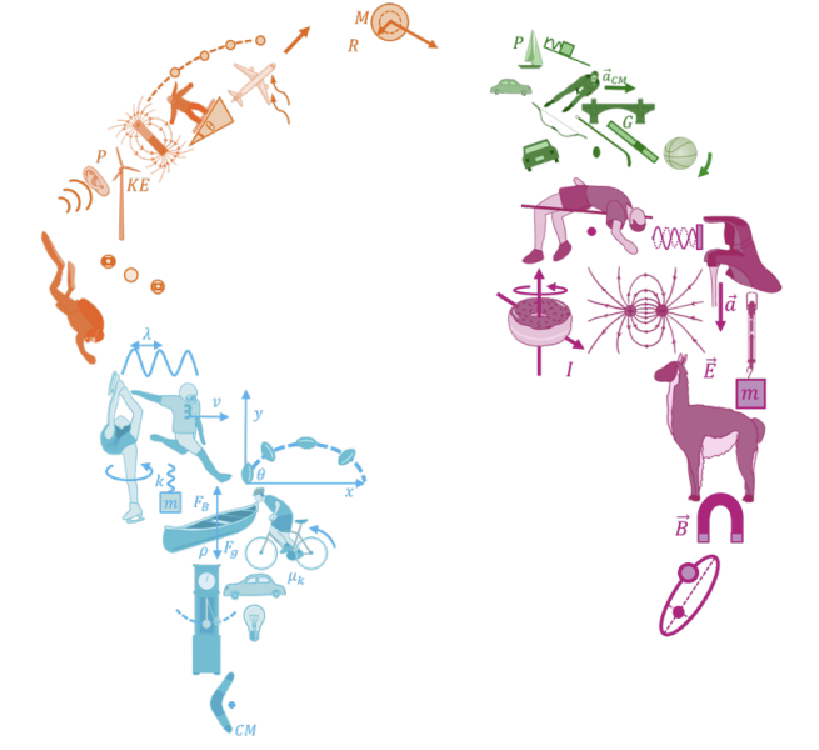
\includegraphics[width=4cm]{figures/BMDW/logo}
\end{textblock*}

\end{frame}

%%%%%%%%%%%%%TOC
\twocolframe{Outline}
  {\tableofcontents[sections={55,56}, subsectionstyle=show/show]\thispagestyle{empty}}
  {\tableofcontents[sections={57}, subsectionstyle=show/show]}
%%%%%%%%%%%%%%%%%%%%%%%%%







%%%%%%%%%%%%%%%%%%%%%%%%%%%%%%%%
\section{Modeling Circuits}
\label{sec:modelingcircuits}
\title{Modeling Circuits}


%%%%%%%%%%%%%%%%%%%%%%%%%
\begin{frame}
\titlepage
\thispagestyle{empty}
\end{frame}


%%%%%%%%%%%%%%%%%%%%%%%%



\def\proton at (#1,#2,#3){
\draw[fill=black,opacity=1] (#1,#2) circle (#3);
% a plus sign that scales
\draw[color=white] (#1-0.8*#3,#2) -- (#1+0.8*#3,#2);
\draw[color=white] (#1,#2-0.8*#3) -- (#1,#2+0.8*#3);
}

\def\ion at (#1,#2,#3){
\draw[fill=orange,opacity=1,draw=orange] (#1,#2) circle (#3);
% a plus sign that scales
\draw[color=white] (#1-0.8*#3,#2) -- (#1+0.8*#3,#2);
\draw[color=white] (#1,#2-0.8*#3) -- (#1,#2+0.8*#3);
}

\def\electron at (#1,#2,#3){
\fill[color=myred,opacity=1] (#1,#2) circle (#3);
% a minus sign that scales
\draw[color=white] (#1-0.8*#3,#2) -- (#1+0.8*#3,#2);
}

%%%%%%%%%%%%%%%%%%%%%%%%%%%%%%
\subsection{The electric cell}
\label{subsec:thelectriccell}
\twocolframe{The electric cell}
{
\begin{itemize}
\item Zinc ``likes'' to be dissolved as an ion in acid.
\item The zinc ions leave their electrons behind in the electrode, making the zinc electrode negatively charged.
\item Electrons that are loosely bound in a carbon electrode are attracted into the electrolyte solution, leaving the carbon electrode positively charged.
\item Very quickly, the process stops as an equilibrium is reached, with a net electric potential difference between electrodes.
\end{itemize}
}
{ 
\begin{center}

\begin{tikzpicture}[scale=1]
\tikzmath{
\Lou=2.0;
\Lw=1.0;
\Rou=1.5;
\dr=0.07;
\fac=0.3;
\Rd=0.17;
\Ld=3.3;
\xs=0.7;
\rp=0.1;
\re=0.05;
}  

\scalebox{1}{
%liquid:
  \fill[color=myblue!80,opacity=0.5] (-\Rou,0) arc (180:360:{\Rou} and {\fac*\Rou}) --  (\Rou,0)-- (\Rou, \Lw) arc (0:-180:{\Rou} and {\fac*\Rou}) -- (-\Rou,\Lw); 
  \fill[color=myblue!60, opacity=0.5] (\Rou,\Lw) arc (0:360:{\Rou} and {\fac*\Rou}) ;
 \draw[color=black] (\Rou,\Lw) arc (0:180:{\Rou} and {\fac*\Rou}) ;

%BACK RIM OF CONTAINER
  \draw[color=myblue!50, color=black, opacity=1, name path=A1] (\Rou,\Lou) arc (0:180:{\Rou} and {\fac*\Rou}) ;
  \draw[color=myblue!20, color=black, opacity=1, name path=B1] (\Rou-\dr,\Lou) arc (0:180:{\Rou-\dr} and {\fac*(\Rou-\dr)});
  \tikzfillbetween[of=A1 and B1]{gray}; 
  
%Rods:
  \fill[color=black!70,opacity=0.9] (-\Rd-\xs,0) arc (180:360:{\Rd} and {\fac*\Rd}) --  (\Rd-\xs,0)-- (\Rd-\xs, \Ld) arc (0:-180:{\Rd} and {\fac*\Rd}) -- (-\Rd-\xs,\Ld); 
  \fill[color=black!70, opacity=0.9] (\Rd-\xs,\Ld) arc (0:360:{\Rd} and {\fac*\Rd}) ;
  %\draw[color=black, dashed] (\Rd-\xs,\Lw) arc (0:360:{\Rd} and {\fac*\Rd}) ;
  \fill[color=myblue!50, opacity=0.5] (\Rd-\xs,\Lw) arc (0:-180:{\Rd} and {\fac*\Rd})  -- (-\xs-\Rd,\Lw-0.95) -- (-\xs+\Rd,\Lw-1.07);
    
  \fill[color=orange!80, opacity=0.9] (-\Rd+\xs,0) arc (180:360:{\Rd} and {\fac*\Rd}) --  (\Rd+\xs,0)-- (\Rd+\xs, \Ld) arc (0:-180:{\Rd} and {\fac*\Rd}) -- (-\Rd+\xs,\Ld); 
  \fill[color=orange!80, opacity=0.9] (\Rd+\xs,\Ld) arc (0:360:{\Rd} and {\fac*\Rd}) ;
  %\draw[color=orange, dashed] (\Rd+\xs,\Lw) arc (0:360:{\Rd} and {\fac*\Rd}) ;
  \fill[color=myblue!50, opacity=0.5] (\Rd+\xs,\Lw) arc (0:-180:{\Rd} and {\fac*\Rd})-- (\xs-\Rd,\Lw-1.07)  -- (\xs+\Rd,\Lw-0.95) ;
   
  \draw[color=black] (\Rou,\Lw) arc (0:-180:{\Rou} and {\fac*\Rou}) ;
   
%% particles
  \foreach \i in {1,3,...,7} {
   \proton at (-\xs-0.05,\i*\Ld/7-0.5,1.1*\rp)
   \electron at (\xs-0.07,\i*\Ld/7-0.5,1.1*\re)
  } 
  \foreach \i in {2,4,...,7} {
   \proton at (-\xs+0.07,\i*\Ld/7-0.5,0.9*\rp)
   \electron at (\xs+0.07,\i*\Ld/7-0.5,0.9*\re)
  } 
  
  \ion at (\xs-1.8*\Rd,1.3,0.9*\rp)
  \ion at (\xs-3*\Rd,1.2,0.9*\rp)
  \ion at (\xs-2*\Rd,\Ld/7-0.5,0.9*\rp)
  \ion at (\xs-2*\Rd,0.2,0.9*\rp)
  \ion at (\xs-3.2*\Rd,\Ld/7-0.7,\rp)
  \ion at (\xs-4*\Rd,0,1.1*\rp)
  \ion at (\xs-4.5*\Rd,\Ld/7-0.5,1.1*\rp)
  
  \electron at (-\xs+1.2*\Rd,\Ld/7-0.5,0.9*\re)
  \electron at (-\xs+2*\Rd,0.2,0.9*\re)
  \electron at (-\xs+2*\Rd,0.6,0.9*\re)
  \electron at (-\xs+1.7*\Rd,1.2,1.1*\re)
  \electron at (-\xs+2.8*\Rd,\Ld/7-0.7,\re)
  \electron at (-\xs+3*\Rd,0.4,1.1*\re)
  \electron at (-\xs+2.5*\Rd,\Ld/7,\re)
          
%front of container:
  \fill[left color=gray,right color=gray!20,shading=axis,opacity=0.2, draw=black] (-\Rou,0) arc (180:360:{\Rou} and {\fac*\Rou}) --  (\Rou,0)-- (\Rou, \Lou) arc (0:-180:{\Rou} and {\fac*\Rou}) -- (-\Rou,\Lou); 
  \draw[color=myblue!50, color=black, opacity=1, name path=A2] (\Rou,\Lou) arc (0:-180:{\Rou} and {\fac*\Rou}) ;
  \draw[color=myblue!20, color=black, opacity=1, name path=B2] (\Rou-\dr,\Lou) arc (0:-180:{\Rou-\dr} and {\fac*(\Rou-\dr)});
  \tikzfillbetween[of=A2 and B2]{gray}; 
 
 
 \node[above, left=2pt] at (-\Rd-\xs,\Ld){{Carbon rod (+)}};
 \node[above, right=8pt] at (-\Rd+\xs,\Ld){{Zinc rod (-)}};
 \draw[color=myred,-latex](-\Rou,-0.6*\Rou/2)  node[below=-4pt] {{electrons}}  -- (-\xs+2.8*\Rd,\Ld/7-0.7,\re);
 \draw[-latex](-1.1*\Rou,0)  node[left=1pt] {{Carbon ions}}  -- (-\xs-1.1*\Rd,\Ld/7-0.5);
 \draw[color=orange,-latex](\Rou,-0.6*\Rou/2)  node[below=-4pt] {{zinc ions}}  -- (\xs-2*\Rd,0.2);
 \draw[-latex] (-1.2*\Rou,\Lou/2) -- (-0.8*\Rou,\Lou/2);
 \node[left=5pt] at (-\Rou,\Lou/2) {{Electrolyte}};  
 \draw[latex-latex] (-\xs,1.05*\Ld) -- (\xs,1.05*\Ld) node[above,midway] {{$\Delta V$}}; 
 }
\end{tikzpicture}
\captionof*{figure}{\textit{An electric cell made with an electrolyte, such as $H_2SO_4$ (sulfuric acid) and two metals.}}
\end{center}
}


%%%%%%%%%%%%%%%%%%%%%%%%%%%%%%



%%%%%%%%%%%%%%%%%%%%%%%%%%%%%%
\subsection{Current flow in a battery}
\label{subsec:currentflowinabattery}
\twocolframesf{Current flow in a battery}
{
\begin{itemize}
\item The rate of chemical reactions in the battery limits the current that can be produced. 
\item The components of the battery themselves will have a finite resistance (e.g. the rods). 
\item If the resistance of the resistor (and battery) is low enough, the rate of chemical reactions cannot sustain the current implied by Ohm's Law ($V=RI$). The voltage of the battery thus drops until the current given by Ohm's Law can be sustained by the chemical reactions.
\end{itemize}
}
{
\begin{tikzpicture}[scale=0.3]
  \def\Lou{6.0}
  \def\Lw{3.0}
  \def\Rou{4}
  \def\dr{0.2}
  \def\fac{0.3}
  \def\Rd{0.5}
  \def\Ld{10}
  \def\xs{2}
  \def\rp{0.3}
  \def\re{0.15}
  
%liquid:
  \fill[color=myblue!80,opacity=0.5] (-\Rou,0) arc (180:360:{\Rou} and {\fac*\Rou}) --  (\Rou,0)-- (\Rou, \Lw) arc (0:-180:{\Rou} and {\fac*\Rou}) -- (-\Rou,\Lw); 
  \fill[color=myblue!60, opacity=0.5] (\Rou,\Lw) arc (0:360:{\Rou} and {\fac*\Rou}) ;
 \draw[color=black] (\Rou,\Lw) arc (0:180:{\Rou} and {\fac*\Rou}) ;

%BACK RIM OF CONTAINER
  \draw[color=myblue!50, color=black, opacity=1, name path=A1] (\Rou,\Lou) arc (0:180:{\Rou} and {\fac*\Rou}) ;
  \draw[color=myblue!20, color=black, opacity=1, name path=B1] (\Rou-\dr,\Lou) arc (0:180:{\Rou-\dr} and {\fac*(\Rou-\dr)});
  \tikzfillbetween[of=A1 and B1]{gray}; 
  

%Rods:
  \fill[color=black!70,opacity=0.9] (-\Rd-\xs,0) arc (180:360:{\Rd} and {\fac*\Rd}) --  (\Rd-\xs,0)-- (\Rd-\xs, \Ld) arc (0:-180:{\Rd} and {\fac*\Rd}) -- (-\Rd-\xs,\Ld); 
  \fill[color=black!70, opacity=0.9] (\Rd-\xs,\Ld) arc (0:360:{\Rd} and {\fac*\Rd}) ;
  \fill[color=myblue!50, opacity=0.5] (\Rd-\xs,\Lw) arc (0:-180:{\Rd} and {\fac*\Rd})  -- (-\xs-\Rd,\Lw-0.95) -- (-\xs+\Rd,\Lw-1.07);
    
  \fill[color=orange!80, opacity=0.9] (-\Rd+\xs,0) arc (180:360:{\Rd} and {\fac*\Rd}) --  (\Rd+\xs,0)-- (\Rd+\xs, \Ld) arc (0:-180:{\Rd} and {\fac*\Rd}) -- (-\Rd+\xs,\Ld); 
  \fill[color=orange!80, opacity=0.9] (\Rd+\xs,\Ld) arc (0:360:{\Rd} and {\fac*\Rd}) ;
  \fill[color=myblue!50, opacity=0.5] (\Rd+\xs,\Lw) arc (0:-180:{\Rd} and {\fac*\Rd})-- (\xs-\Rd,\Lw-1.07)  -- (\xs+\Rd,\Lw-0.95) ;
   
  \draw[color=black] (\Rou,\Lw) arc (0:-180:{\Rou} and {\fac*\Rou}) ;
   
%% particles
  \foreach \i in {1,3,...,7} {
   \proton at (-\xs-0.15,\i*\Ld/7-0.5,1.1*\rp)
   \electron at (\xs-0.2,\i*\Ld/7-1,1.1*\re)
   \draw [-latex,color=myred] (\xs-0.2,\i*\Ld/7-1+1.1*\re)--(\xs-0.2,\i*\Ld/7-1+1.1*\re+0.7);
   
  } 
  \foreach \i in {2,4,...,7} {
   \proton at (-\xs+0.2,\i*\Ld/7-0.5,0.9*\rp)
   \electron at (\xs+0.2,\i*\Ld/7-1,0.9*\re)
   \draw [-latex,color=myred] (\xs+0.2,\i*\Ld/7-1+0.9*\re)--(\xs+0.2,\i*\Ld/7-1+0.9*\re+0.7);
  } 
  
  \ion at (\xs-1.8*\Rd,1.3,0.9*\rp)
  \ion at (\xs-3*\Rd,1.2,0.9*\rp)
  \ion at (\xs-2*\Rd,\Ld/7-0.5,0.9*\rp)
  \ion at (\xs-2*\Rd,0.2,0.9*\rp)
  \ion at (\xs-3.2*\Rd,\Ld/7-0.7,\rp)
  \ion at (\xs-4*\Rd,0,1.1*\rp)
  \ion at (\xs-4.5*\Rd,\Ld/7-0.5,1.1*\rp)
  \ion at (\xs-5*\Rd,-0.2,1.1*\rp)
  \ion at (\xs-2.7*\Rd,0,\rp)
  
  \electron at (-\xs+1.2*\Rd,\Ld/7-0.5,0.9*\re)
  \electron at (-\xs+2*\Rd,0.2,0.9*\re)
  \electron at (-\xs+2*\Rd,0.6,0.9*\re)
  \electron at (-\xs+1.7*\Rd,1.2,1.1*\re)
  \electron at (-\xs+2.8*\Rd,\Ld/7-0.7,\re)
  \electron at (-\xs+3*\Rd,0.4,1.1*\re)
  \electron at (-\xs+2.5*\Rd,\Ld/7,\re)
  %\electron at (-\xs+4*\Rd,0.6,1.1*\re)
  %\electron at (-\xs+3.7*\Rd,1.4,1.1*\re)    
%front of container:
  \fill[left color=gray,right color=gray!20,shading=axis,opacity=0.2, draw=black] (-\Rou,0) arc (180:360:{\Rou} and {\fac*\Rou}) --  (\Rou,0)-- (\Rou, \Lou) arc (0:-180:{\Rou} and {\fac*\Rou}) -- (-\Rou,\Lou); 
  \draw[color=myblue!50, color=black, opacity=1, name path=A2] (\Rou,\Lou) arc (0:-180:{\Rou} and {\fac*\Rou}) ;
  \draw[color=myblue!20, color=black, opacity=1, name path=B2] (\Rou-\dr,\Lou) arc (0:-180:{\Rou-\dr} and {\fac*(\Rou-\dr)});
  \tikzfillbetween[of=A2 and B2]{gray}; 
 
 %resistor
 \draw[line width=8pt,black!30=qred!] (-\xs,1.05*\Ld) -- (\xs,1.05*\Ld) node[above,midway,color=black] {\tiny{$R$}}; 
 \electron at (\xs-1.8*\Rd,1.05*\Ld,1.1*\re)
 \draw [-latex,color=myred] (\xs-1.8*\Rd-1.1*\re,1.05*\Ld) -- (\xs-1.8*\Rd-1.1*\re-0.7,1.05*\Ld);
 \electron at (\xs-5*\Rd,1.05*\Ld,1.1*\re)
 \draw [-latex,color=myred] (\xs-5*\Rd-1.1*\re,1.05*\Ld) -- (\xs-5*\Rd-1.1*\re-0.7,1.05*\Ld);
 
 
 \node[above, left=2pt] at (-\Rd-\xs,\Ld){\tiny{Carbon rod (+)}};
 \node[above, right=8pt] at (-\Rd+\xs,\Ld){\tiny{Zinc rod (-)}};
 \draw[color=myred,-latex](-\Rou,-0.6*\Rou/2)  node[below=-4pt] {\tiny{electrons}}  -- (-\xs+2*\Rd,0.2);
 \draw[-latex](-1.1*\Rou,0)  node[left=1pt] {\tiny{Carbon ions}}  -- (-\xs-1.1*\Rd,\Ld/7-0.5);
 \draw[color=orange,-latex](\Rou,-0.6*\Rou/2)  node[below=-4pt] {\tiny{zinc ions}}  -- (\xs-2*\Rd,0.2);
 \draw[-latex] (-1.2*\Rou,\Lou/2) -- (-0.8*\Rou,\Lou/2);
 \node[left=5pt] at (-\Rou,\Lou/2) {\tiny{Electrolyte}};  
 \draw[-latex] (-0.5*\xs,0.95*\Ld) -- (0.5*\xs,0.95*\Ld) node[midway,below]{\tiny{$I$}};
\end{tikzpicture}
\captionof*{figure}{\textit{As electrons leave the zinc, more ions can dissolve. They eventually neutralize in the solution as electrons come in through the carbon.}}
}



%%%%%%%%%%%%%%%%%%%%%%%%%%%%%%
\subsection{Modeling a real battery}
\label{subsec:modelingarealbattery}
\twocolframesf{Modeling a real battery}
{

\begin{itemize}
\item We can model a real battery as an ideal battery + a resistor (``internal resistance'').
\item The ``emf'', $\epsilon$, is the potential difference of the ideal battery:
\begin{itemize}
 \item It is a constant, independent of what we connect to the battery.
 \item ``Internal voltage'' of the battery, if you prefer a better description than ``electromotive force''.
\end{itemize}
\item The ``terminal voltage'' is the actual voltage measured at the external terminals of the battery. It \textit{depends on the current flowing through the battery} (which results in a voltage drop across the internal resistance, $r$).
\end{itemize}
}
{
\centering
\begin{circuitikz}[scale=0.2]
\def\h{6}
\def\L{20}
\def\w{12}
\def\Rt{1}
\def\fs{0.6}

%rectangular prism
\fill[top color=myred!20,bottom color=myred!80,shading=axis,opacity=0.8, draw=black] (0,0,0) -- (0,\h,0) -- (\L,\h,0) -- (\L, 0, 0); 
\fill[top color=myred!80,bottom color=myred!20,shading=axis,opacity=0.8, draw=black] (0,\h,0) --(0,\h,-\w) -- (\L,\h,-\w) -- (\L, \h, 0); 
\fill[top color=myred!20,bottom color=myred!80,shading=axis,opacity=0.8, draw=black] (\L, 0, 0) --  (\L, \h, 0) -- (\L,\h,-\w) --(\L,0,-\w); 


%battery terminals (by stacking circles!)
\foreach \i in {0,0.05,...,0.5} {
  \begin{scope}[canvas is xz plane at y=\h+\i]
    \fill (0.15*\L,-\w/2) circle(\Rt);
    \fill (0.85*\L,-\w/2) circle(\Rt);
  \end{scope}
}
%circuit components
\scalebox{\fs}{
  \begin{scope}[canvas is xz plane at y=\h/\fs]
    \draw (0.15*\L/\fs,-\w/2/\fs) [short,thick] to (0.3*\L/\fs,-\w/2/\fs)
     to [R,thick] (0.5*\L/\fs,-\w/2/\fs)
     to [battery1={$\,$},thick] (0.7*\L/\fs,-\w/2/\fs)
     to [short,thick] (0.85*\L/\fs,-\w/2/\fs);
  \end{scope}
}

\node[above=-3pt,color=white] at (0.22*\L,\h,0) {\small A};
\node[above=-3pt,color=white] at (0.92*\L,\h,0) {\small B};
\node[above=-3pt] at (0.7*\L+0.25,\h,0) {{\textbf{$\epsilon$}}};
\node[above=-3pt] at (0.5*\L,\h,0) {\small{\textbf{$r$}}};
\draw[latex-latex] (0.28*\L,2*\h) -- (0.95*\L,2*\h) node[above,midway] {\small{Terminal voltage, $V_{AB}$}}; 

\end{circuitikz}
\captionof*{figure}{\textit{A real battery, modelled with an internal resistance.}}
}


%%%%%%%%%%%%%%%%%%%%%%%%%%%%%%



%%%%%%%%%%%%%%%%%%%%%%%%%%%%%%
\subsection{Terminal voltage in a real ciruit}
\label{subsec:terminalvoltageinarealcircuit}
\twocolframesf{Terminal voltage in a real circuit}
{

\begin{itemize}
\item The current through both resistors is \SI{3}{A}.% 
\item The voltage drop across a resistor, $V=RI$:
\begin{itemize}
\item The voltage drop across the \SI{2}{\Omega} resistor is $(\SI{2}{\Omega})(\SI{3}{A})=\SI{6}{V}$
\item The voltage drop across the \SI{1}{\Omega} resistor is $(\SI{1}{\Omega})(\SI{3}{A})=\SI{3}{V}$
\end{itemize}
\item We identify that the “terminal voltage” is between the $-$ terminal ($B$) of the ideal battery, and the point between the two resistors ($A$)
\item The terminal voltage is $V=\SI{9}{V}-\SI{6}{V}=\SI{3}{V}$
\textit{assuming the internal battery can sustain $\SI{3}{A}$}.
\end{itemize}
With a larger resistor, $R$, the total current would be smaller and the voltage drop across $r$ negligible. 
}
{
\vspace{-2cm}
\centering
\begin{tikzpicture}[scale=0.15]
\def\h{6}
\def\L{20}
\def\w{12}
\def\Rt{1}
\def\fs{0.4}

%rectangular prism
\fill[top color=myred!20,bottom color=myred!80,shading=axis,opacity=0.8, draw=black] (0,0,0) -- (0,\h,0) -- (\L,\h,0) -- (\L, 0, 0); 
\fill[top color=myred!80,bottom color=myred!20,shading=axis,opacity=0.8, draw=black] (0,\h,0) --(0,\h,-\w) -- (\L,\h,-\w) -- (\L, \h, 0); 
\fill[top color=myred!20,bottom color=myred!80,shading=axis,opacity=0.8, draw=black] (\L, 0, 0) --  (\L, \h, 0) -- (\L,\h,-\w) --(\L,0,-\w); 

%battery terminals (by stacking circles!)
\foreach \i in {0,0.05,...,0.5} {
  \begin{scope}[canvas is xz plane at y=\h+\i]
    \fill (0.15*\L,-\w/2) circle(\Rt);
    \fill (0.85*\L,-\w/2) circle(\Rt);
  \end{scope}
}
%circuit components
\scalebox{\fs}{
  \begin{scope}[canvas is xz plane at y=\h/\fs]
    \draw (0.15*\L/\fs,-\w/2/\fs) [short,thick] to (0.3*\L/\fs,-\w/2/\fs)
     to [R,thick] (0.5*\L/\fs,-\w/2/\fs)
     to [battery1={$\,$},thick] (0.7*\L/\fs,-\w/2/\fs)
     to [short,thick] (0.85*\L/\fs,-\w/2/\fs);
  \end{scope}
}

%wire
\draw[] (0.15*\L,\h,-\w/2) -- (0.15*\L,2.*\h,-\w/2) -- (0.85*\L,2.*\h,-\w/2) node[midway, above] {$R$} -- (0.85*\L,\h,-\w/2);

\node[above=-3pt,color=white] at (0.22*\L,\h,0) {A};
\node[above=-3pt,color=white] at (0.92*\L,\h,0) {B};
\node[above=-3pt] at (0.7*\L+0.25,\h,0) {{\textbf{$\epsilon$}}};
\node[above=-3pt] at (0.5*\L,\h,0) {{\textbf{$r$}}};

\end{tikzpicture}%

\captionof*{figure}{\textit{A battery shorted with a wire of resistance, $R$}}%

\vspace{-0.7cm}
\begin{circuitikz}
\scalebox{0.85}
{
\def\h{2}
\def\L{4}

 \draw (0,0)  [battery1={$\,$},l^=$\epsilon$,-*,i=$I$] to (\L,0) node[below] {B};
 \draw (\L,0) [short] to (\L,\h)
       to [R,l_=$R\;(\SI{1}{\Omega})$,-*] (0.5*\L,\h) node[above] {A}
       to [R,l_=$r\;(\SI{2}{\Omega})$,] (0,\h)
       to [short] (0,0);
       
 \node[color=myred] at (0.25*\L,0.75*\h) {$\SI{6}{V}$};
 \node[color=myred] at (0.5*\L,0.75*\h) {$+$};
 \node[color=myred] at (0.75*\L,0.75*\h) {$\SI{3}{V}$};
 \node[color=myred] at (0.5*\L,-0.3*\h) {$\SI{9}{V}$};
}
\end{circuitikz}%
\captionof*{figure}{\textit{Circuit diagram for the shorted battery. The current is $I=\frac{\SI{9}{V}}{(\SI{2}{\Omega})+(\SI{4}{\Omega})}=\SI{3}{A}$}}%
}


%%%%%%%%%%%%%%%%%%%%%%%%%%%%%%



%%%%%%%%%%%%%%%%%%%%%%%%%%%%%%
\subsection{Analysing ciruits}
\label{subsec:analysingciruits}
\twocolframe{Analysing circuits}
{
\begin{itemize}
\item  If you know the currents through all of the resistors in a circuit, you know everything that there is to know about the circuit:
\begin{itemize}
\item  Given the currents in all resistors, you can calculate the voltage across each of the resistors.
\end{itemize}
\item  Usually, the easiest method to do this is to combine resistors together into equivalent resistors.
\item  However, this cannot always be done, in particular, when the circuit contains more than one battery.
\end{itemize}
}
{\begin{circuitikz}[scale=0.7]
\scalebox{1}
{
\def\h{2}
\def\L{4}

 \draw (-\L,0) node[below] {f}   [battery1,l_={$V_1=\SI{24}{V}$},*-*] to (0,0);
 \draw (-\L,0) to [short,-*] (-\L,\L) node[above] {a}
       to [R,l_={$R_1=\SI{3}{\Omega}$},-*] (0,\L) node[above] {b}
       to [R,l_={$R_2=\SI{3}{\Omega}$}] (0,0) node[below] {e} ;
 \draw (0,0)  [battery1,l_={$V_2=\SI{29}{V}$},*-,invert] to (\L,0) node[below] {d};
 \draw (\L,0) to [R,l^={$R_4=\SI{4}{\Omega}$},-*]  (\L,\L) node[above] {c}
       to [R,l^={$R_3=\SI{3}{\Omega}$}] (0,\L);             

 
 \draw[-latex,color=qblue,line width = 2] (-\L,0.75*\h)--+(0,1) node[midway,left]{$I_1$};
 \draw[-latex,color=qblue,line width = 2] (-0.3*\L,2*\h)--+(1,0) node[midway,above]{$I_1$};
 \draw[-latex,color=qblue,line width = 2] (-0.09*\L,0)--+(-1,0) node[midway,above]{$I_1$};

 \draw[-latex,color=qblue,line width = 2] (0.07*\L,2*\h)--+(1,0) node[midway,above]{$I_2$};
  \draw[-latex,color=qblue,line width = 2] (\L,1.9*\h)--+(0,-1) node[midway,right]{$I_2$};
  \draw[-latex,color=qblue,line width = 2] (0.3*\L,0)--+(-1,0) node[midway,above]{$I_2$};

  \draw[-latex,color=qblue,line width = 2] (0,1.9*\h)--+(0,-1) node[midway,right]{$I_3$};
  \draw[-latex,color=qblue,line width = 2] (0,0.6*\h)--+(0,-1) node[midway,left]{$I_3$}; 
}
\end{circuitikz}%
\captionof*{figure}{\textit{We would like to know all of the currents in this circuit. It cannot be simplified to a single equivalent resistor.}}%
}



%%%%%%%%%%%%%%%%%%%%%%%%%%%%%%
\subsection{Analogies for circuits}
\label{subsec:analogiesforcircuits}
\begin{frame}{A not so great analogy}%
 \begin{columns} %
 \column{0.5\textwidth}%
 \centering%
 \begin{circuitikz}[scale=0.7]%
\scalebox{1}%
{%
\def\h{2}%
\draw (\h,0) [battery1=$\Delta V$] to (-\h,0);%
\draw (-\h,0) [short] to (-\h,\h);%
\draw (-\h,\h) [R,l_=$R$] to (\h,\h);%
\draw (\h,\h) [short] to (\h,0);%
}%
\end{circuitikz}%
 \column{0.5\textwidth}%
 \capfig{0.9}{figures/Circuits/rollercoaster}{https://en.wikipedia.org/wiki/File:Ednör\_–\_L\%27Attaque\_-\_panoramio.jpg}%
 \begin{tikzpicture}[remember picture,overlay]%
 \fill[color=white] ($(current page.center)+(4.5cm,2cm)$) rectangle +(1cm,0.6cm);%
 \node[color=qred, above] at ($(current page.center)+(5cm,2cm)$) {\Large $\Delta V$};%
 \fill[color=white] ($(current page.center)+(0.8cm,2cm)$) rectangle +(0.5cm,0.6cm);%
 \node[color=qred, above] at ($(current page.center)+(1cm,2cm)$) {\Large $R$};%
 \end{tikzpicture}%
 \end{columns}%
\begin{itemize}%
\item Often, the analogy between a circuit and a roller coaster is made:%
\begin{itemize}%
\item The battery acts like the lift for the train, giving it potential energy.%
\item The train then looses its potential energy by going down the track, which is like the resistor.%
\end{itemize}
\item Why is this not a great analogy?%
\end{itemize}
\end{frame}


%%%%%%%%%%%%%%%%%%%%%%%%%%%%%%
\twocolframe{A better analogy}
{
\begin{itemize}
\item  If the charges are like the cars on a roller coaster, the battery is the lift
that brings them up the hill.
\item  When they go down the hill, the key difference with a roller coaster is that
they arrive at the bottom with zero speed (they lost all of their energy in the resistor $\rightarrow$ like a paddle wheel).
\end{itemize}
}
{

\only<1>{
\capfig{0.8}{figures/Circuits/tex/currentcoaster_series_page1}{Charges ``lose'' their energy as heat in the resistors.}
}

\only<2>{
\capfig{0.8}{figures/Circuits/tex/currentcoaster_series_page2}{With resistors in series, the same current goes through each resistor, and the potential energy is shared between the two.}
}

\only<3>{
\centering
\animategraphics[autoplay,loop,width=5cm]{10}{figures/Circuits/animgif/series-}{0}{2}
}

\only<4>{
\capfig{0.8}{figures/Circuits/tex/currentcoaster_series_page3}{With resistors in parallel, there is less current through each resistor but the same amount of potential energy.}
}

\only<5>{
\centering
\animategraphics[autoplay,loop,width=5cm]{10}{figures/Circuits/animgif/parallel-}{0}{5}
}

}


%%%%%%%%%%%%%%%%%%%%%%%%%%%%%%
\twocolframefs{Or even better}
{
\begin{itemize}
\item Change in pressure drives the water in a pipe.
\item The resistance to water flow in the pipe depends on how long and how narrow the pipe is:
\begin{itemize}
\item Longer $\rightarrow$ more resistance.
\item Wider $\rightarrow$ less resistance.
\end{itemize}
\item Just like a resistor:
\begin{align*}
R\rho \frac{L}{A}
\end{align*} 
\end{itemize}
}
{
\begin{columns}
\column{0.5\textwidth}
\begin{circuitikz}[scale=0.7]%
  \scalebox{1}%
  {%
  \def\h{2}%
  \draw (\h,0) [battery1=$\Delta V$] to (-\h,0);%
  \draw (-\h,0) [short] to (-\h,\h);%
  \draw (-\h,\h) [R,l_=$R$] to (\h,\h);%
  \draw (\h,\h) [short] to (\h,0);%
  \draw[-latex, line width=2.5, color=qred] (0.5,0) -- (1.5,0) node[above, midway]{$I$};
  }%
\end{circuitikz}%
\captionof*{figure}{\textit{Current is driven through the resistor by a potential difference. The current is the same everywhere in the wire (continuity).}}%

\column{0.5\textwidth}
  \begin{tikzpicture}[scale=0.7]%
  \scalebox{1}%
  {%
  \def\h{2.5}%
  \def\fac{0.8}
  \def\zer{0.2}
  %\fill[color=myblue!40,rounded corners=10] (-\h,0) -- (-\h,\h) -- (\h,\h) --(\h,0) ;
  %\fill[color=white,rounded corners=10] (-\fac*\h,\zer*\h) -- (-{\fac*\h},\fac*\h) -- (\fac*\h,\fac*\h) --(\fac*\h,\zer*\h) --(-\fac*\h,\zer*\h) ;
  \fill[color=myblue!40,rounded corners=10]  (-\h,0) rectangle (\h,\h) ;
  \fill[color=white,rounded corners=10] (-\fac*\h,\zer*\h) rectangle (\fac*\h,\fac*\h) ;
  \fill[color=myblue!40] (0,\zer/2.0*\h) circle(\h/4);
  
  \fill[color=white,rounded corners=10] (-\h/2,0.5*\fac*\h) rectangle (\h/2,1.1*\fac*\h) ;
  \fill[color=white,rounded corners=10] (-\h/2,1.1*\fac*\h+0.2*\zer*\h) rectangle (\h/2,2*\fac*\h) ;
  
  \node[below=10pt] at (0,0) {$\Delta P$};
  \node[above=5pt] at (0,\h) {$R$};
  \draw[-latex, line width=2.5, color=qred] (0.5,\zer/2.0*\h) -- (1.5,\zer/2.0*\h) node[above, midway]{$Q$};

  }%
\end{tikzpicture}%
\captionof*{figure}{\textit{Fluid is driven through the resistor by a difference in pressure (e.g. from a pump). The flow rate is the same everywhere in the pipe (continuity).}}%

\end{columns}

}

%%%%%%%%%%%%%%%%%%%%%%%%%%%%%%
\twocolframesf{Kirchhoff's rules}
{
\begin{itemize}
\item \textbf{Charge conservation:}
\begin{itemize}
\item Charges cannot just appear or disappear from a circuit, they have to go somewhere (there is nowhere for water to enter or leave a closed system).
\end{itemize}
\item \textbf{Energy conservation:}
\begin{itemize}
\item If a charge moves around a loop in a circuit, its energy must not change (the water does not flow faster and faster in a closed system).
\end{itemize}
\end{itemize}
}
{
\capfig{0.6}{figures/Circuits/fountain}{A garden fountain is a closed system. There are multiple paths for the water to go down (resistors in parallel). Since there is no paddle wheel, what is the water’s kinetic energy being converted to?}
}

%%%%%%%%%%%%%%%%%%%%%%%%%%%%%%




\section{Kirchoff's Laws}
\label{sec:kirchoffslaws}
\title{Kirchoff's Laws}


%%%%%%%%%%%%%%%%%%%%%%%%%
\begin{frame}
\titlepage
\thispagestyle{empty}
\end{frame}




%%%%%%%%%%%%%%%%%%%%%%%%%%%%
\subsection{Kirchoff's rules}
\label{subsec:kirchoffsrules}
\twocolframe{Kirchhoff's rules}
{
\begin{itemize}
\item \textbf{Junction rule} (charge):
\begin{itemize}
\item The sum of the currents coming into a junction
must equal the sum of the currents coming out of a
junction:
\begin{align*}
\text{incoming current} &= \text{outgoing current}\\
I_1+I_2+I_4 &= I_3+I_5
\end{align*}
\end{itemize}
\item \textbf{Loop rule} (energy):
\begin{itemize}
\item The sum of the potential differences in any closed loop must be zero:
\begin{align*}
V_1+V_2+V_3+\Delta V=0
\end{align*}
\end{itemize}
\end{itemize}
}
{
\vspace{-0.5cm}
\centering
 \begin{circuitikz}[scale=0.7]%
\scalebox{1}%
{%
\def\h{2.5}%
\draw (45:\h) [short,i=$I_1$] to (0,0);%
\draw (95:\h) [short,i=$I_2$] to (0,0);%
\draw (0,0) [short,i=$I_3$] to (145:\h);%\\
\draw (210:\h) [short,i=$I_4$] to (0,0);%
\draw (0,0) [short,i=$I_5$] to (290:\h);%
\fill (0,0) circle(2pt);
}%
\end{circuitikz}%
\captionof*{figure}{\textit{The junction rule.}}%

 \begin{circuitikz}[scale=0.7]%
\scalebox{1}%
{%
\def\h{1.4}%
\draw (3*\h,0) [battery1=$\Delta V$,-*] to (-3*\h,0);%
\draw (-3*\h,0) [short,-*] to (-3*\h,\h);%
\draw (-3*\h,\h) [R,l^={$V_1=IR_1$},-*] to (-1*\h,\h);
\draw (-1*\h,\h) [R,l^={$V_2=IR_2$},-*] to (1*\h,\h);
\draw (1*\h,\h) [R,l^={$V_3=IR_3$},-*] to (3*\h,\h) ;%
\draw (3*\h,\h) [short,-*] to (3*\h,0);%
}%
\end{circuitikz}%
\captionof*{figure}{\textit{The loop rule.}}%

}


%%%%%%%%%%%%%%%%%%%%%%%%%%%%%%
\subsection{Using Kirchoff's laws}
\twocolframe{Using Kirchhoff's Laws}
{
Getting started
\begin{enumerate}
\item Make a well-labeled diagram.
\item Identify the junctions.
\item Identify the loops.
\end{enumerate}
}
{
\begin{circuitikz}[scale=0.7]
\scalebox{1}
{
\def\h{2}
\def\L{4}

 \draw (-\L,0) node[below] {f}   [battery1,l_={$V_1=\SI{24}{V}$},*-*] to (0,0);
 \draw (-\L,0) to [short,-*] (-\L,\L) node[above] {a}
       to [R,l_={$R_1=\SI{3}{\Omega}$},-*] (0,\L) node[above] {b}
       to [R,l_={$R_2=\SI{3}{\Omega}$}] (0,0) node[below] {e} ;
 \draw (0,0)  [battery1,l_={$V_2=\SI{29}{V}$},*-,invert] to (\L,0) node[below] {d};
 \draw (\L,0) to [R,l^={$R_4=\SI{4}{\Omega}$},-*]  (\L,\L) node[above] {c}
       to [R,l^={$R_3=\SI{3}{\Omega}$}] (0,\L);             

}
\end{circuitikz}%
\captionof*{figure}{\textit{We would like to know all of the currents in this circuit.}}%
}




%%%%%%%%%%%%%%%%%%%%%%%%%%%%%%



%%%%%%%%%%%%%%%%%%%%%%%%%%%%%%

\twocolframe{Using Kirchhoff's Laws}
{
\begin{enumerate}
\item Draw a good diagram with nodes labeled.
\item<2-> Draw ``battery arrows'' from $-$ to $+$.
\item<3-> Make a \textbf{consistent} \emph{guess} for currents.
\only<4-9>{:
\begin{itemize}
\item Start \textit{anywhere} and keep introducing a new current each time you hit a junction.
\end{itemize}
}
\item<10-> Write the Junction Rule (once per junction, up to $N-1$ for $N$ junctions):
\begin{align*}
\boxed{I_1=I_2+I_3}
\end{align*}
Expect 3 unknowns, so need 2 more equations... The loop equations!
\end{enumerate}

}
{
\begin{circuitikz}[scale=0.75]
\scalebox{1}
{
\def\h{2}
\def\L{4}

 \draw (-\L,0) node[below] {f}   [battery1,l_={$V_1=\SI{24}{V}$},*-*] to (0,0);
 \draw (-\L,0) to [short,-*] (-\L,\L) node[above] {a}
       to [R,l_={$R_1=\SI{3}{\Omega}$},-*] (0,\L) node[above] {b}
       to [R,l_={$R_2=\SI{3}{\Omega}$}] (0,0) node[below] {e} ;
 \draw (0,0)  [battery1,l_={$V_2=\SI{29}{V}$},*-,invert] to (\L,0) node[below] {d};
 \draw (\L,0) to [R,l^={$R_4=\SI{4}{\Omega}$},-*]  (\L,\L) node[above] {c}
       to [R,l^={$R_3=\SI{3}{\Omega}$}] (0,\L);             
\only<2->{
 \draw [-latex,color=qred,line width = 4] (-0.4*\L,\h/3+0.2)-- +(-1,0);
 \draw [-latex,color=qred,line width = 4] (0.4*\L,\h/3+0.2)-- +(1,0);
 }

 \only<4->{
 \fill[color=qred] (-\L,0) circle(0.1);
 \draw[-latex,color=qblue,line width = 2] (-\L,0.75*\h)--+(0,1) node[midway,left]{$I_1$};
 } 
 \only<5->{
 \draw[-latex,color=qblue,line width = 2] (-0.95*\L,2*\h)--+(1,0) node[midway,above]{$I_1$};
 \draw[-latex,color=qblue,line width = 2] (-0.3*\L,2*\h)--+(1,0) node[midway,above]{$I_1$};
 \fill[color=qred] (0,2*\h) circle(0.1);
 } 
 \only<6->{
 \draw[-latex,color=qblue,line width = 2] (0.07*\L,2*\h)--+(1,0) node[midway,above]{$I_2$};
  \draw[-latex,color=qblue,line width = 2] (0,1.9*\h)--+(0,-1) node[midway,left]{$I_3$};
 }
 \only<7->{
  \draw[-latex,color=qblue,line width = 2] (0.7*\L,2*\h)--+(1,0) node[midway,above]{$I_2$};
  \draw[-latex,color=qblue,line width = 2] (\L,1.9*\h)--+(0,-1) node[midway,right]{$I_2$};
  \draw[-latex,color=qblue,line width = 2] (\L,0.6*\h)--+(0,-1) node[midway,right]{$I_2$};
  \draw[-latex,color=qblue,line width = 2] (0.95*\L,0)--+(-1,0) node[midway,above]{$I_2$};
  \draw[-latex,color=qblue,line width = 2] (0.3*\L,0)--+(-1,0) node[midway,above]{$I_2$};
 }
 \only<8->{
  \draw[-latex,color=qblue,line width = 2] (0,0.6*\h)--+(0,-1) node[midway,left]{$I_3$};
  \fill[color=qred] (0,0) circle(0.1);
 }
  \only<9->{
  \draw[-latex,color=qblue,line width = 2] (-0.09*\L,0)--+(-1,0) node[midway,above]{$I_1$};
  \draw[-latex,color=qblue,line width = 2] (-0.7*\L,0)--+(-1,0) node[midway,above]{$I_1$};
 }
}
\end{circuitikz}%
\captionof*{figure}{\textit{We want to know all current in this circuit diagram.}}%
}


%%%%%%%%%%%%%%%%%%%%%%%%%%%%%%
\twocolframe{The loop equations}
{
\begin{itemize}
\item \textbf{Important}: \textit{You choose} which way to “walk” around the loop. It’s completely arbitrary. Two rules:
\begin{enumerate}
\item When you encounter a \textbf{\textcolor{qred}{battery arrow: Add the voltage}} if you walk in the same direction as the arrow, subtract otherwise.
\item  When you encounter a \textbf{\textcolor{qblue}{resistor: Subtract the voltage}} across the resistor if you walk in the same direction as the current, add otherwise
\end{enumerate}
\item Across a closed loop, the voltage must be zero.
\end{itemize}

}
{
\begin{circuitikz}[scale=0.75]
\scalebox{1}
{
\def\h{2}
\def\L{4}

 \draw (-\L,0) node[below] {f}   [battery1,l_={$V_1=\SI{24}{V}$},*-*] to (0,0);
 \draw (-\L,0) to [short,-*] (-\L,\L) node[above] {a}
       to [R,l_={$R_1=\SI{3}{\Omega}$},-*] (0,\L) node[above] {b}
       to [R,l_={$R_2=\SI{3}{\Omega}$}] (0,0) node[below] {e} ;
 \draw (0,0)  [battery1,l_={$V_2=\SI{29}{V}$},*-,invert] to (\L,0) node[below] {d};
 \draw (\L,0) to [R,l^={$R_4=\SI{4}{\Omega}$},-*]  (\L,\L) node[above] {c}
       to [R,l^={$R_3=\SI{3}{\Omega}$}] (0,\L);             

 \draw [-latex,color=qred,line width = 4] (-0.4*\L,\h/3)-- +(-1,0);
 \draw [-latex,color=qred,line width = 4] (0.4*\L,\h/3)-- +(1,0);
 


 \draw[-latex,color=qblue,line width = 2] (-\L,0.75*\h)--+(0,1) node[midway,left]{$I_1$};
 \draw[-latex,color=qblue,line width = 2] (-0.3*\L,2*\h)--+(1,0) node[midway,above]{$I_1$};
 \draw[-latex,color=qblue,line width = 2] (-0.09*\L,0)--+(-1,0) node[midway,above]{$I_1$};

 \draw[-latex,color=qblue,line width = 2] (0.07*\L,2*\h)--+(1,0) node[midway,above]{$I_2$};
  \draw[-latex,color=qblue,line width = 2] (\L,1.9*\h)--+(0,-1) node[midway,right]{$I_2$};
  \draw[-latex,color=qblue,line width = 2] (0.3*\L,0)--+(-1,0) node[midway,above]{$I_2$};

  \draw[-latex,color=qblue,line width = 2] (0,1.9*\h)--+(0,-1) node[midway,right]{$I_3$};
  \draw[-latex,color=qblue,line width = 2] (0,0.6*\h)--+(0,-1) node[midway,left]{$I_3$}; 
}
\end{circuitikz}%
\captionof*{figure}{\textit{Circuit diagram with everything well-labeled.}}%
}


%%%%%%%%%%%%%%%%%%%%%%%%%%%%%%
%%%%%%%%%%%%%%%%%%%%%%%%%%%%%%%%%%%





\section{Solving Circuits}
\label{sec:solvingcircuits}
\title{Solving Circuits}


%%%%%%%%%%%%%%%%%%%%%%%%%
\begin{frame}
\titlepage
\thispagestyle{empty}
\end{frame}





%%%%%%%%%%%%%%%%%%%%%%%%%%%%%%%%%
\subsection{Loop equations}
\label{subsec:loopequations}
\twocolframe{The loop equations}
{

\begin{itemize}
\item[$\rightarrow$] Consider loop $abcdefa$:
\only<2>{
\item(ab): with current, $I_1$ through resistor $R_1$: \textcolor{qred}{$-R_1I_1 \rightarrow -3I_1$}
}
\only<3>{ 
\item(bc): with current, $I_2$ through resistor $R_3$: \textcolor{qred}{$-R_3I_2 \rightarrow -3I_2$}
}
\only<4>{ 
\item(cd): with current, $I_2$ through resistor $R_4$: \textcolor{qred}{$-R_3I_2 \rightarrow -4I_2$}
}
\only<5>{ 
\item(de): \textit{against} battery arrow: \textcolor{qred}{$-V_2 \rightarrow -29$}
}
\only<6>{ 
\item(ef): with battery arrow: \textcolor{qred}{$+V_1 \rightarrow +24$}
}
\only<7>{ 
\item(fa): no battery or resistor, so no voltage change. Back to starting point: \textcolor{qred}{$=0$}
}
\only<8>{
\item We now have a second equation (recall that there are 3 unknowns). We need one more loop equation. 
}

\end{itemize}

}
{
\begin{circuitikz}[scale=0.7]
\scalebox{1}
{
\def\h{2}
\def\L{4}

\only<1,2,8>{
\draw[color=qred!50, line width=6,-latex] (-\L,2*\h) -- (0,2*\h) node[midway,above] {\reflectbox{
\includegraphics[scale=.4]{figures/Circuits/girl}}};
}
\only<1,3,8>{
\draw[color=qred!50, line width=6,-latex] (0,2*\h) -- (\L,2*\h)  node[midway,above] {\reflectbox{
\includegraphics[scale=.4]{figures/Circuits/girl}}};
}
\only<1,4,8>{
\draw[color=qred!50, line width=6,-latex] (\L,2*\h) -- (\L,0) node[rotate=-90,midway,above] {\reflectbox{
\includegraphics[scale=.4]{figures/Circuits/girl}}};
}
\only<1,5,8>{
\draw[color=qred!50, line width=6,-latex] (\L,0) -- (0,0)node[rotate=-180,midway,above] {\reflectbox{
\includegraphics[scale=.4]{figures/Circuits/girl}}};
}
\only<1,6,8>{
\draw[color=qred!50, line width=6,-latex] (0,0) -- (-\L,0)node[rotate=-180,midway,above] {\reflectbox{
\includegraphics[scale=.4]{figures/Circuits/girl}}};
}
\only<1,7,8>{
\draw[color=qred!50, line width=6,-latex] (-\L,0) -- (-\L,2*\h)node[rotate=-270,midway,above] {\reflectbox{
\includegraphics[scale=.4]{figures/Circuits/girl}}};
}

 \draw (-\L,0) node[below] {f}   [battery1,l_={$V_1=\SI{24}{V}$},*-*] to (0,0);
 \draw (-\L,0) to [short,-*] (-\L,\L) node[above] {a}
       to [R,l_={$R_1=\SI{3}{\Omega}$},-*] (0,\L) node[above] {b}
       to [R,l_={$R_2=\SI{3}{\Omega}$}] (0,0) node[below] {e} ;
 \draw (0,0)  [battery1,l_={$V_2=\SI{29}{V}$},*-,invert] to (\L,0) node[below] {d};
 \draw (\L,0) to [R,l^={$R_4=\SI{4}{\Omega}$},-*]  (\L,\L) node[above] {c}
       to [R,l^={$R_3=\SI{3}{\Omega}$}] (0,\L);             

 \draw [-latex,color=qred,line width = 4] (-0.4*\L,\h/3+0.2)-- +(-1,0);
 \draw [-latex,color=qred,line width = 4] (0.4*\L,\h/3+0.2)-- +(1,0);
 


 \draw[-latex,color=qblue,line width = 2] (-\L,0.75*\h)--+(0,1) node[midway,left]{$I_1$};
 \draw[-latex,color=qblue,line width = 2] (-0.3*\L,2*\h)--+(1,0) node[midway,above]{$I_1$};
 \draw[-latex,color=qblue,line width = 2] (-0.09*\L,0)--+(-1,0) node[midway,above]{$I_1$};

 \draw[-latex,color=qblue,line width = 2] (0.07*\L,2*\h)--+(1,0) node[midway,above]{$I_2$};
  \draw[-latex,color=qblue,line width = 2] (\L,1.9*\h)--+(0,-1) node[midway,right]{$I_2$};
  \draw[-latex,color=qblue,line width = 2] (0.3*\L,0)--+(-1,0) node[midway,above]{$I_2$};

  \draw[-latex,color=qblue,line width = 2] (0,1.9*\h)--+(0,-1) node[midway,right]{$I_3$};
  \draw[-latex,color=qblue,line width = 2] (0,0.6*\h)--+(0,-1) node[midway,left]{$I_3$}; 
}
\end{circuitikz}%
\captionof*{figure}{\textit{Going around loop $(abcdefa)$.}}%
\only<2>{
Equation for loop ($abcdefa$):
\begin{align*}
 \textcolor{qred}{-3I_1}\dots
\end{align*}
}
\only<3>{
Equation for loop ($abcdefa$):
\begin{align*}
 -3I_1\textcolor{qred}{\;-3I_2}\dots
\end{align*}
}
\only<4>{
Equation for loop ($abcdefa$):
\begin{align*}
 -3I_1-3I_2\textcolor{qred}{\;-4I_2}\dots
\end{align*}
}
\only<5>{
Equation for loop ($abcdefa$):
\begin{align*}
 -3I_1-3I_2-4I_2\textcolor{qred}{\;-29}\dots
\end{align*}
}
\only<6>{
Equation for loop ($abcdefa$):
\begin{align*}
 -3I_1-3I_2-4I_2-29\textcolor{qred}{\;+24}\dots
\end{align*}
}
\only<7>{
Equation for loop ($abcdefa$):
\begin{align*}
 -3I_1-3I_2-4I_2-29+24\textcolor{qred}{\;=0}
\end{align*}
}
\only<8>{
Equation for loop ($abcdefa$):
\begin{align*}
\therefore -3I_1-3I_2-4I_2-29+24=0
\end{align*}
}

}





%%%%%%%%%%%%%%%%%%%%%%%%%%%%%%
\twocolframe{The loop equations}
{
\begin{itemize}
\item Choose loop $bcdeb$:
\begin{itemize}
\item (bc): $-R_3I_2 \rightarrow -3I_2$ (with current through resistor)
\item (cd): $-R_4I_2 \rightarrow -4I_2$ (with current through resistor)
\item (de): $-V_2 \rightarrow -29$ (\textit{against} battery arrow)
\item (eb): $+R_2I_3 \rightarrow +3I_3$ (\textit{against} current through resistor)
\end{itemize}
\end{itemize}
}
{
\begin{circuitikz}[scale=0.75]
\scalebox{1}
{
\def\h{2}
\def\L{4}

\draw[color=qred!50, line width=6,-latex] (0,2*\h) -- (\L,2*\h);
\draw[color=qred!50, line width=6,-latex] (\L,2*\h) -- (\L,0);
\draw[color=qred!50, line width=6,-latex] (\L,0) -- (0,0);
\draw[color=qred!50, line width=6,-latex] (0,0) -- (0,2*\h);

 \draw (-\L,0) node[below] {f}   [battery1,l_={$V_1=\SI{24}{V}$},*-*] to (0,0);
 \draw (-\L,0) to [short,-*] (-\L,\L) node[above] {a}
       to [R,l_={$R_1=\SI{3}{\Omega}$},-*] (0,\L) node[above] {b}
       to [R,l_={$R_2=\SI{3}{\Omega}$}] (0,0) node[below] {e} ;
 \draw (0,0)  [battery1,l_={$V_2=\SI{29}{V}$},*-,invert] to (\L,0) node[below] {d};
 \draw (\L,0) to [R,l^={$R_4=\SI{4}{\Omega}$},-*]  (\L,\L) node[above] {c}
       to [R,l^={$R_3=\SI{3}{\Omega}$}] (0,\L);             

 \draw [-latex,color=qred,line width = 4] (-0.4*\L,\h/3+0.2)-- +(-1,0);
 \draw [-latex,color=qred,line width = 4] (0.4*\L,\h/3+0.2)-- +(1,0);
 
 \draw[-latex,color=qblue,line width = 2] (-\L,0.75*\h)--+(0,1) node[midway,left]{$I_1$};
 \draw[-latex,color=qblue,line width = 2] (-0.3*\L,2*\h)--+(1,0) node[midway,above]{$I_1$};
 \draw[-latex,color=qblue,line width = 2] (-0.09*\L,0)--+(-1,0) node[midway,above]{$I_1$};

 \draw[-latex,color=qblue,line width = 2] (0.07*\L,2*\h)--+(1,0) node[midway,above]{$I_2$};
  \draw[-latex,color=qblue,line width = 2] (\L,1.9*\h)--+(0,-1) node[midway,right]{$I_2$};
  \draw[-latex,color=qblue,line width = 2] (0.3*\L,0)--+(-1,0) node[midway,above]{$I_2$};

  \draw[-latex,color=qblue,line width = 2] (0,1.9*\h)--+(0,-1) node[midway,right]{$I_3$};
  \draw[-latex,color=qblue,line width = 2] (0,0.6*\h)--+(0,-1) node[midway,left]{$I_3$}; 
}
\end{circuitikz}%
\captionof*{figure}{\textit{Circuit diagram with loop $(bcdeb)$ highlighted.}}%

Equation for loop ($bcdeb$):
\begin{align*}
\therefore -3I_2-4I_2-29+3I_3=0
\end{align*}
}



%%%%%%%%%%%%%%%%%%%%%%%%%%%%%%
\subsection{Solving circuits using loop equations}
\label{subsec:solvingcircuitsusingloopequations}
\twocolframe{Solving the circuit}
{
\begin{itemize}
\item We now have 3 equations and 3 unknowns, allowing us to determine all of the currents.
\begin{align*}
I_2+I_3&=I_1 &\text{(Junction rule)}\\
-3I_1-3I_2-4I_2-29+24&=0 &\text{(Loop abcdefa)}\\
-3I_2-4I_2-29+3I_3&=0 &\text{(Loop bcdeb)}
\end{align*}
\item The system of linear equations is easier to handle if you don't include the units (so make sure everything is in SI units!).
\end{itemize}
}
{
\begin{circuitikz}[scale=0.7]
\scalebox{1}
{
\def\h{2}
\def\L{4}

 \draw (-\L,0) node[below] {f}   [battery1,l_={$V_1=\SI{24}{V}$},*-*] to (0,0);
 \draw (-\L,0) to [short,-*] (-\L,\L) node[above] {a}
       to [R,l_={$R_1=\SI{3}{\Omega}$},-*] (0,\L) node[above] {b}
       to [R,l_={$R_2=\SI{3}{\Omega}$}] (0,0) node[below] {e} ;
 \draw (0,0)  [battery1,l_={$V_2=\SI{29}{V}$},*-,invert] to (\L,0) node[below] {d};
 \draw (\L,0) to [R,l^={$R_4=\SI{4}{\Omega}$},-*]  (\L,\L) node[above] {c}
       to [R,l^={$R_3=\SI{3}{\Omega}$}] (0,\L);             

 \draw [-latex,color=qred,line width = 4] (-0.4*\L,\h/3+0.2)-- +(-1,0);
 \draw [-latex,color=qred,line width = 4] (0.4*\L,\h/3+0.2)-- +(1,0);
 
 \draw[-latex,color=qblue,line width = 2] (-\L,0.75*\h)--+(0,1) node[midway,left]{$I_1$};
 \draw[-latex,color=qblue,line width = 2] (-0.3*\L,2*\h)--+(1,0) node[midway,above]{$I_1$};
 \draw[-latex,color=qblue,line width = 2] (-0.09*\L,0)--+(-1,0) node[midway,above]{$I_1$};

 \draw[-latex,color=qblue,line width = 2] (0.07*\L,2*\h)--+(1,0) node[midway,above]{$I_2$};
  \draw[-latex,color=qblue,line width = 2] (\L,1.9*\h)--+(0,-1) node[midway,right]{$I_2$};
  \draw[-latex,color=qblue,line width = 2] (0.3*\L,0)--+(-1,0) node[midway,above]{$I_2$};

  \draw[-latex,color=qblue,line width = 2] (0,1.9*\h)--+(0,-1) node[midway,right]{$I_3$};
  \draw[-latex,color=qblue,line width = 2] (0,0.6*\h)--+(0,-1) node[midway,left]{$I_3$}; 
}
\end{circuitikz}%
\captionof*{figure}{\textit{Well-labeled circuit diagram.}}%
}


%%%%%%%%%%%%%%%%%%%%%%%%%%%%%%
\subsection{Solving a ciruit - foolproof method!}
\label{subsec:solcingacircuitfoolproofmethod}
\twocolframesf{Solving a circuit - Foolproof method!}
{
\begin{enumerate}
\item Make a good diagram.
\item Simplify resistors that can be combined.
\item Draw ``battery arrows'', from $-$ to $+$ (small slide to big side).
\item Guess currents in a consistent manner (start somewhere and proceed).
\item Write the junction rule equations (once per junction).
\item Write the loop equations.
\item Solve $N$ equations for $N$ unknown currents.
\end{enumerate}
}
{
\vspace{-1.75cm}
\vspace{-1cm}
\begin{exampleblock}{Direction of current(s)}
It is possible that you find negative values for the current(s). In that case, \textbf{first, solve for all of the other currents}. Then, \textit{at the very end}, reverse the arrows in the diagram since you guessed the direction wrong (but in a consistent way!).
\end{exampleblock}
}


%%%%%%%%%%%%%%%%%%%%%%%%%%%%%%





%%%%%%%%%%%%%%%%%%%%%%%%%%%%%%%


\subsection{The galvanometer}
\label{subsec:thegalvanometer}
\twocolframe{The galvanometer}
{
\begin{itemize}
\item As we will learn, a wire that carries a current will feel a force if placed in a magnetic field.
\item A galvanometer is a very sensitive device for measuring current.
\item Typically, they measure currents of order micro amperes.
\item Can obviously use to measure current.
\item Can also use to measure voltage.
\end{itemize}
}
{
\capfig{1}{figures/Circuits/galvanometer}{A galvanometer}
}

%%%%%%%%%%%%%%%%%%%%%%%%%%%%%%
\subsection{Measuring current}
\label{subsec:measuringcurrent}
\twocolframe{Measuring current}
{
\begin{itemize}
\only<1>{
\item Based on using a galvanometer:
\begin{itemize}
\item[$\rightarrow$] Need to have a very small current through the galvanometer
\end{itemize}
\item An \textbf{ammeter} measures currents, even potentially large ones.
\item We thus add a resistor in \textbf{parallel} with a galvanometer to create an ammeter.
\item This is called a \textit{shunt} resistor.
}
\only<2>{
\item We know the current through the galvanometer and the value of all resistors.
The total current is:
\begin{align*}
I=I_G+I_s
\end{align*}
\item Both resistors have the same potential difference:
\begin{align*}
R_GI_G=R_sI_s
\end{align*}
\item The total current, in terms of $I_G$, is thus:
\begin{align*}
I=I_G+I_s=I_G\left( 1 + \frac{R_G}{R_s}\right)
\end{align*}
}
\end{itemize}
}
{
\centering
 \begin{circuitikz}[scale=0.7]%
\scalebox{1}%
{%
\def\h{1.5}%
\draw (-1.5*\h,0) [short,*-] to (0,0);

\draw (0,0) [short] to (0,\h);
\draw (0,\h) [rmeter,t=G] to (2*\h,\h);
\draw (2*\h,\h) [short] to (2*\h,0);

\draw (0,0) [short] to (0,-\h);
\draw (0,-\h) [R=$R_s$] to (2*\h,-\h);
\draw (2*\h,-\h) [short] to (2*\h,0);

\draw (2*\h,0) [short,-*] to (3.5*\h,0);

\draw[dotted, color=qblue!70, line width=2] (-0.3*\h ,-1.3*\h) rectangle(2.3*\h ,1.6*\h) node [above=7pt,left] {Ammeter};


\draw[color=qred, line width=1pt, -latex] (-1.7,0) -- +(1,0) node[midway, above] {$I$};
\draw[color=qred, line width=1pt, -latex] (3.9,0) -- +(1,0) node[midway, above] {$I$};
\draw[color=qred, line width=1pt, -latex] (0,0.2) -- +(0,1) node[midway, right] {$I_G$};
\draw[color=qred, line width=1pt, -latex] (0,-0.2) -- +(0,-1) node[midway, right] {$I_s$};
 
 }%
\end{circuitikz}%
\captionof*{figure}{\textit{An ammeter made using a galvanometer and a (small) shunt resistor. Most of the current goes through the shunt. An ammeter is connected in series and has a very low resistance.}}%

}

%%%%%%%%%%%%%%%%%%%%%%%%%%%%%%
\subsection{Measuring Voltage}
\twocolframe{Measuring Voltage}
{
\begin{itemize}
\item Again, we need a small current through the galvanometer, but would like to measure a large potential difference.
\item We place a large resistor in \textbf{series} with the galvanometer.
\item Both see the same current, so if R is large it will have the biggest potential difference.
\begin{align*}
\Delta V = I_G(R + R_G)
\end{align*}
\end{itemize}
}
{
\centering
 \begin{circuitikz}[scale=0.7]%
\scalebox{1}%
{%
\def\h{1.5}%
\draw (-1.0*\h,0) [short,*-] to (0,0);
\draw (0,0) [R=$R$] to (2*\h,0);
\draw (2*\h,0) [rmeter,t=G] to (3.0*\h,0);
\draw (3.0*\h,0) [short,-*] to (4.0*\h,0);

\draw[dotted, color=qblue!70, line width=2] (-0.2*\h,-0.7*\h) rectangle(3.2*\h ,1*\h) node [above=7pt,left] {Voltmeter};

\draw[color=qred, line width=1pt, -latex] (-1.4,0) -- +(1,0) node[midway, above] {$I_G$};
\draw[latex-latex, line width=1.5pt] (-\h,-\h) -- (4*\h,-\h) node[midway,below] {$\Delta V$};
}
\end{circuitikz}%
\captionof*{figure}{\textit{A voltmeter made using a galvanometer and a (large) resistor in series. Most of the voltage drop happens across the large resistor, $R$. A voltmeter is connected in parallel and has a very large resistance.}}%
}

%%%%%%%%%%%%%%%%%%%%%%%%%%%%%%
\subsection{The multimeter}
\label{subsec:themultimeter}
\twocolframesf{The multimeter}
{
\begin{itemize}
\item Can measure current, voltage and resistance.
\item The knob chooses the value of the resistor and its configuration.
\item To measure resistance, the device has an internal voltage source; it then measures the current across a resistor connected across it leads (the resistor cannot be connected to anything else).
\end{itemize}
}
{
\capfig{0.9}{figures/Circuits/multimeter}{https://www.amazon.ca/Digital-Multimeter-Voltmeter-Ohmmeter-Detachable/dp/B08K3G2GRF}
}


\subsection{RC circuits}
\label{subsec:rccircuits}
\twocolframesf{RC Circuits}
{
\begin{itemize}
\item Consider a circuit with a resistor and a capacitor:
\begin{itemize}
\item Current cannot flow through a capacitor.
\item Capacitor charges up with time, until current is zero.
\item[$\rightarrow$] The current in an RC circuit is not constant!
\end{itemize}
Consider the loop rule (recall $Q=CV$ for a capacitor:
\begin{align*}
\Delta V - IR - \frac{Q}{C} &=0\\
\Delta V - \frac{dQ}{dt}R - \frac{Q}{C} &=0\\
\therefore Q(t) &= C\Delta V\left (1-e^{-\frac{t}{RC}}\right)
\end{align*} 

\end{itemize}

}
{
\vspace{-1cm}
\begin{center}
\begin{circuitikz}
 \draw (0,0) to [short] (0,2)
       to [R=$R$] (2,2)
       to [C=$C$] (4,2)
       to [nos, l_=S] (4,0)
       to [battery1,v^=$\Delta V$] (0,0);        
\end{circuitikz}
\captionof*{figure}{\label{fig:circuits:RCcircuit}\textit{ A simple circuit with a resistor, battery, and capacitor.}} 
\end{center}
When the switch is closed, current decreases exponentially with time:
\begin{align*}
I(t) = \frac{dQ}{dt} = \frac{\Delta V}{R} e^{-\frac{t}{RC}}
\end{align*}
}


%%%%%%%%%%%%%%%%%%%%%%%%%%%%%%%























%%%%%%%%%%%%%%%%%%%%%%%%%%%%%%%%%




\title{Magnetic Force}
\subject{Magnetic Force, Fields and Torques}
\subtitle{Building Models to Describe our World}


%%%%%%%%%%%%%%%%%%%%%%%%%%%%%%
%%%%%%%%%%%%%%%%%%%%%




%%%%%%%%%%%%%%%%%%%%%%%%%
%%%%%% Title slide %%%%%%
%%%%%%%%%%%%%%%%%%%%%%%%%
\chaptertitle{Magnetic Force}
\begin{frame}
\label{chap:magneticforce}
\titlepage
\thispagestyle{empty}

\begin{textblock*}{5cm}(11cm,4cm)
    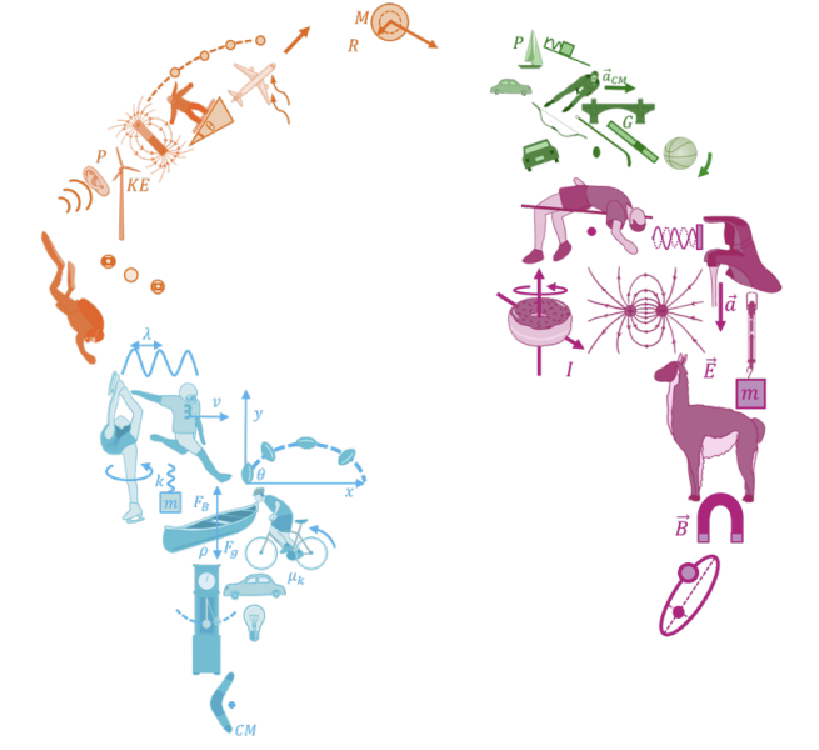
\includegraphics[width=4cm]{figures/BMDW/logo}
\end{textblock*}

\end{frame}

%%%%%%%%%%%%%TOC
\twocolframe{Outline}
  {\tableofcontents[sections={58,59}, subsectionstyle=show/show]\thispagestyle{empty}}
  {\tableofcontents[sections={60}, subsectionstyle=show/show]}
%%%%%%%%%%%%%%%%%%%%%%%%%







%%%%%%%%%%%%%%%%%%%%%%%%%%%%%%%%
\section{The Magnetic Force}
\label{sec:themagneticforce}
\title{The Magnetic Force}


%%%%%%%%%%%%%%%%%%%%%%%%%
\begin{frame}
\titlepage
\thispagestyle{empty}
\end{frame}

%







%%%%%%%%%%%%%%%%%%%%%%%%%%%%%%%
\subsection{Magnetism Basics}
\label{subsec:magnetism}
\twocolframest{Magnetism}
{
\begin{itemize}
\item Some rocks were found to be ``magnetic'' (rather, they were found to attract and repel each other, and they came from a place called Magnesia); ``lodestone''.
\item If you make a needle out of a piece of magnetic material, and suspend it, it kind of points towards the geographic North Pole of the Earth.
\item We call a piece of magnetic material a ``magnet''. We label the side that points towards Earth’s North Pole, the North side of the magnet (cause it points North).
\end{itemize}
}
{
\vspace{-0.5cm}
\capfig{0.75}{figures/Bforce/rock}{https://en.wikipedia.org/wiki/Lodestone}
\vspace{-0.75cm}
\capfig{0.75}{figures/Bforce/compass}{https://www.walmart.ca/en/ip/Pocket-Compass-with-Aluminum-Shell-Edge-for-Outdoor-Camping-Hiking-Sports-Navigation/779N64NE92KJ}
}


%%%%%%%%%%%%%%%%%%%%%%%%%%%%%%

%%%%%%%%%%%%%%%%%%%%%%%%%%%%%%
\begin{bulletframe}{Magnets}
\item With bar magnets, one side (=N) of the magnet always wants to point towards geographic north (ish).
\item We call the other side of the magnet S, since it points to geographic South (ish).
\item It has been observed that the same sides of magnets repel each other (NN or SS), while the opposite sides attract (N-S).
\end{bulletframe}

%%%%%%%%%%%%%%%%%%%%%%%%%%%%%%


%%%%%%%%%%%%%%%%%%%%%%%%%%%%%%
\twocolframesf{Magnetic fields}
{
\vspace{-0.25cm}
\begin{itemize}
\item Fields were introduced as a tool to model ``force at a distance''.
\item Magnetic \textbf{field points in the direction of force on N} (from N to S).
\item Just like electric field lines:
\begin{itemize}
\item Field vector length represented by density of lines.
\item Field vector is tangent to the lines.
\end{itemize}
\item Unlike electric field lines:
\begin{itemize}
\item \textbf{No isolated magnetic charges}, only bar magnets (dipoles).
\item \textbf{Field lines never end}, they are always closed loops.
\end{itemize}
\item The closest analogy with electric charges is that bar magnets are like electric dipoles.
\end{itemize}
}
{
\vspace{-1cm}
\capfig{0.75}{figures/Bforce/edipole}{An electric dipole.}
\vspace{-0.75cm}
\capfig{0.75}{figures/Bforce/barfield}{A magnetic dipole.}
}

%%%%%%%%%%%%%%%%%%%%%%%%%%%%%%




%%%%%%%%%%%%%%%%%%%%%%%%%%%%%%



%%%%%%%%%%%%%%%%%%%%%%%%%%%%%%
\begin{frame}{Cutting up a bar magnet}

\centering
\begin{tikzpicture}{scale=1}
\scalebox{1}
{
\def\L{8}%bar length
\def\h{1.1}%bar height
\def\xs{0.5}%offset
\def\mar{0.3}%margin for N/S label

 \foreach \fac [count=\i] in {1,2,4}
 {
   \def\l{\L/\fac} 
   \def\yb{-\i*\h*1.3}
 
   \foreach \j in {1,...,\fac}{
   \def\xl{-\L/2+(\j-1)*(\l+\xs)-\xs*(\fac-1)/2}
   \fill[left color=qred, right color=qblue, shading=axis,opacity=0.3] ({\xl},\yb-\h/2) rectangle ({\xl+\l}, \yb+\h/2);
   \node at ({\xl+\mar},\yb) {N};
   \node at ({\xl+\l-\mar},\yb) {S};
   }
 }
}
\end{tikzpicture}%
\captionof*{figure}{\textit{When we cut a magnet in 2, we get another magnet (with N and S) sides.}}%
\end{frame}


%%%%%%%%%%%%%%%%%%%%%%%%%%%%%%
\twocolframesf{Tiny bar magnets}
{
\begin{itemize}
\item You can think of magnetic materials as being made up of tiny little bar magnets.
\item The fields for those ``tiny bar magnets'' add up to make the field from a large bar magnet.
\item Those tiny little bar magnets ultimately come from electrons spinning around in atoms:
\begin{itemize}
\item As we will see in next chapter, moving charges create magnetic fields.
\item The electrons spin around the atom.
\item The electrons also spin about their own axis (this is actually the main contribution, and it's Quantum Mechanics).
\end{itemize}
\end{itemize}
}
{
\vspace{-1.2cm}
\capfig{0.75}{figures/Bforce/loopfield}{Magnetic field from a loop of current.}
\vspace{-0.5cm}
\capfig{0.75}{figures/Bforce/barfield}{Magnetic field from a bar magnet.}
}

%%%%%%%%%%%%%%%%%%%%%%%%%%%%%%


%%%%%%%%%%%%%%%%%%%%%%%%%%%%%%
\subsection{Recall: vector-cross product}
\twocolframest{Recall: vector cross-product}
{
\begin{itemize}
\item If we have two vectors, $\vec a$ and $\vec b$, we can define the cross-product:
\begin{align*}%
\vec c = \vec a \times \vec b
\end{align*}%
\begin{itemize}
\item $\vec c$ is perpendicular to both $\vec a$ and $\vec b$.
\item  and has magnitude: $c=ab\sin\theta$
\end{itemize}
\item You can always move vectors around, so easiest to draw them tail to tail before taking cross product
\item Use right hand rule to figure which way $\vec c$ points
\end{itemize}
}
{
\centering
\begin{tikzpicture}{scale=1}
\scalebox{1}
{
\draw[-latex, line width=2,color=blue] (0,0) -- (90:2.5) node[midway,right] {$\vec a$};
\draw[-latex, line width=2,color=red] (0,0) -- (140:2) node[midway,below] {$\vec b$};
\draw[line width = 1.] (90:0.8) arc(90:140:0.8) node[midway,above] {$\theta$};
}
\end{tikzpicture}%
\captionof*{figure}{\textit{Vectors, $\vec a$ and $\vec b$. }}%
}



%%%%%%%%%%%%%%%%%%%%%%%%%%%%%%
\subsection{RIght hand rule(s)}
\twocolframesf{Two right-hand rules}
{
\begin{enumerate}
\item A cross-product between two vectors. Right-hand rule for cross-product.
\begin{align*}%
\vec c = \vec a \times \vec b
\end{align*}%
\vspace{1cm}
\item When you need to relate rotation to a vector. Right-hand rule for axial vectors.
\end{enumerate}
}
{
\vspace{-1cm}
\capfig{0.4}{figures/Bforce/hand}{Right-hand rule for cross-product.}
\vspace{-0.5cm}
\capfig{0.4}{figures/Bforce/axishand}{Right-hand rule for axial vectors.}
}



%%%%%%%%%%%%%%%%%%%%%%%%%%%%%%
\subsection{Force on a moving charge}
\label{subsec:forceonamovingcharge}
\begin{bulletframe}{Force on a moving charge}
\item If a moving charge is in a magnetic field, it experiences a force:
\begin{align*}
\vec F = q \vec v \times \vec B
\end{align*}
\item The magnitude of the force is:
\begin{align*}
F=qvB\sin\theta
\end{align*}
\item[$\rightarrow$] We ultimately use this to define the magnetic field (which is clearly not as pretty as for the electric field). That is, we infer $B$ from the magnitude of the force, $F$.
\end{bulletframe}


%%%%%%%%%%%%%%%%%%%%%%%%%%%%%%


%%%%%%%%%%%%%%%%%%%%%%%%%%%%%%



%%%%%%%%%%%%%%%%%%%%%%%%%%%%%%
\begin{bulletframe}{Work done by a constant magnetic field on a moving charge}
\item The force is always perpendicular to the velocity:
\begin{align*}
\vec F = q \vec v \times \vec B
\end{align*}
\item The displacement is always parallel to the velocity, 
\item The force is thus always perpendicular to the displacement (scalar product is 0)
\item[$\rightarrow$] The magnetic force can do no work; it cannot change the kinetic energy. 
\item[$\rightarrow$] The magnetic force can only change the direction of the velocity, not it’s magnitude.
\end{bulletframe}



%%%%%%%%%%%%%%%%%%%%%%%%%%%%%%




%%%%%%%%%%%%%%%%%%%%%%%%%%%%%%
\subsection{Magnetic force on a charged particle}
\label{subsec:magneticforceonachargedparticle}
\twocolframest{Magnetic force on a charged particle}
{
\begin{align*}
\vec F = q \vec v \times \vec B
\end{align*}
\begin{itemize}
\item Some observations:
\begin{itemize}
\item Always perpendicular to both $\vec v$ and $\vec B$ (cross-product).
\item Can do no work.
\item Proportional to electric charge.
\item No magnetic force on a charge at rest.\only<2>{\textcolor{red}{$\rightarrow$ This should make you uncomfortable, why?}}
\end{itemize}
\end{itemize}
}
{
\only<2>{
\capfig{0.6}{figures/Bforce/einstein}{https://en.wikipedia.org/wiki/Albert\_Einstein\_in\_popular\_culture}
}
}


%%%%%%%%%%%%%%%%%%%%%%%%%%%%%%
\twocolframest{FYI Magnetic force on a charged particle}
{
\begin{itemize}
\only<1>{
\item How does the magnetic force know that humans are predominantly right-handed? For example, how would you explain the right-hand rule to an Alien, who has no concept of right and left?}
\only<2>{
\item Remember: There is no such thing as a force, a magnetic field, an electric field, etc. They are all just mathematical constructs. }
\only<3>{
\item Physical Laws cannot depend on humans being right-handed:	
\begin{itemize}
\item We observe that when an electron is near a source of magnetic field (e.g. a current carrying wire), it moves in a certain direction.
\item We use our right hand to define a thing called the magnetic field.
\item We use our right hand again to determine the force from the magnetic field.
\item[$\rightarrow$] Any physical observation (e.g. which way an electron is deflected) depends on using your right hand twice $\rightarrow$ Then, you could also use your left hand, as once you do two cross products, it doesn't matter which hand you used (don't try this at home, unless you are 100\% sure that you understand the argument!)
\end{itemize}
}
\end{itemize}
}
{
}



%%%%%%%%%%%%%%%%%%%%%%%%%%









\begin{bulletframe}{Force on a moving charge}
\item If a moving charge is in a magnetic field, it experiences a force:
\begin{align*}
\vec F = q \vec v \times \vec B
\end{align*}
\item The magnetic force:
\begin{itemize}
\item Only exerted on a moving charge.
\item Does no work.
\item Perpendicular to magnetic field.
\item Perpendicular to velocity.
\item Magnitude: $qvB\sin\theta$.
\item Direction: RHR.
\end{itemize}
\end{bulletframe}

%%%%%%%%%%%%%%%%%%%%%%%%%%%%%%
\subsection{Right hand rule for vector/cross product}
\label{subsec:righthandruleforvector/cross product}
\twocolframesf{Right hand rule for vector/cross product}
{
The cross-product between two vectors. 
\begin{align*}%
\vec c = \vec a \times \vec b
\end{align*}%
\textbf{Magnitude:} $ab\sin\theta$\\
\textbf{Direction:} Right hand rule. The product is always perpendicular to the plane formed by $\vec a$ and $\vec b$. \\
It does not commute:
\begin{align*}
\vec a \times \vec b = -\vec b \times \vec a
\end{align*}
}
{
\vspace{-1cm}
\capfig{1}{figures/Bforce/hand}{Right-hand rule for cross-product.}

}

%%%%%%%%%%%%%%%%%%%%%%%%%%%%%%



%%%%%%%%%%%%%%%%%%%%%%%%%%%%%%






\section{The Magnetic Field}
\label{sec:themagneticfield}
\title{The Magnetic Field}


%%%%%%%%%%%%%%%%%%%%%%%%%
\begin{frame}
\titlepage
\thispagestyle{empty}
\end{frame}





%%%%%%%%%%%%%%%%%%%%%%%
\subsection{Electron in a magnetic field}
\label{subsec:electroninamagneticfield}
\twocolframesf{Electron in a magnetic field}
{
\begin{itemize}
\item<1-> An electron enters a region of space\only<2->{ with a magnetic field perpendicular to its velocity}
\item<2-> The magnetic force is always perpendicular to the velocity:
\only<3->{
\begin{itemize}
\item Speed is constant (no work).
\item Force is constant in magnitude and perpendicular to velocity.
\item[$\rightarrow$] Uniform circular motion:
\begin{align*}
qvB &= m\frac{v^2}{R}\\
\therefore R &= \frac{m}{q}\frac{v}{B}
\end{align*}
\end{itemize}
}
\end{itemize}
\only<4>{
If the electron has a component of velocity in/out of the page, the path will be a helix.
}
}
{
\centering
\begin{tikzpicture}{scale=1}
\scalebox{1}
{
\def\L{5}
\def\h{5}
\def\Ni{9}
\def\Nj{9}
\def\rad{\L/3}

\only<1>{
\fill[qblue!20] (-1.1*\L/2,-1.1*\h/2) rectangle (1.1*\L/2,1.1*\h/2) node[above=5pt, left,color=qblue!80]{Region of space};
}
\only<2->{
\fill[qblue!20] (-1.1*\L/2,-1.1*\h/2) rectangle (1.1*\L/2,1.1*\h/2) node[above=5pt, left,color=qblue!80]{Region of magnetic field};
\node[left=15pt,below=5pt,color=qblue!80] at (1.1*\L/2,1.1*\h/2) {$\vec B$};
}
\foreach \i in {0,...,\Ni}{
  \def\xi{-\L/2+\i*\L/\Ni}
  \foreach \j in {0,...,\Nj}{
    \def\yj{-\h/2+\j*\h/\Ni}
    \only<2->{
    \node[color=qblue!80, opacity=0.8] at (\xi,\yj) {$\odot$};
    }
  }
}

\only<1>{
\draw[line width = 2, color=qred, -latex]  (1.5*\rad,\rad) -- +(-\rad,0) node[above=7pt, right=16pt] {$\vec v$};
}
\only<1->{
\draw[line width = 2, color=qred, -latex]  (0,\rad) -- +(-\rad,0) node[above=7pt, right=8pt] {$\vec v$};
\fill (0,\rad) circle(2pt);
}
\only<2->{
\draw[line width = 2, color=green!50!black, -latex]  (0,\rad) -- (0,0.3*\rad) node[midway, right] {$\vec F_B$};
}

\only<3->{
\draw[line width = 2] (0,0) circle (\rad);
\draw[line width = 2, color=qred, -latex]  (-\rad,0) -- +(0,-\rad) ;
\draw[line width = 2, color=green!50!black, -latex]   (-\rad,0) -- (-0.3*\rad,0) ;

\draw[line width = 2, color=qred, -latex]  (0,-\rad) -- +(\rad,0) ;
\draw[line width = 2, color=green!50!black, -latex]   (0,-\rad) -- (0,-0.3*\rad) ;

\draw[line width = 2, color=qred, -latex]  (\rad,0) -- +(0,\rad) ;
\draw[line width = 2, color=green!50!black, -latex]   (\rad,0) -- (0.3*\rad,0) ;

\draw[dotted, line width =1.5] (0,0) -- (135:\rad) node[midway, above] {$R$};
}

}
\end{tikzpicture}
}

%%%%%%%%%%%%%%%%%%%%%%%%%%%%%%



%%%%%%%%%%%%%%%%%%%%%%%%%%%%%%
\def\electron at (#1,#2,#3){
\fill[color=myred,opacity=0.8] (#1,#2) circle (#3);
\draw[color=white] (#1-0.8*#3,#2) -- (#1+0.8*#3,#2); %+ sign
\draw[color=white] (#1,#2-0.8*#3) -- (#1,#2+0.8*#3); %+ sign
\draw[color=myred,-latex] (#1,#2+#3) -- (#1,#2+3.5*#3);
}

\def\belectron at (#1,#2,#3){
\fill[color=myred,opacity=0.8] (#1,#2) circle (#3);
\draw[color=white] (#1-0.8*#3,#2) -- (#1+0.8*#3,#2); %+ sign
\draw[color=white] (#1,#2-0.8*#3) -- (#1,#2+0.8*#3); %+ sign
\draw[color=myred,-latex] (#1,#2+#3) -- (#1,#2+3.5*#3);
\draw[color=green!50!black,-latex, line width=1pt] (#1-#3,#2) -- (#1-5*#3,#2);
}

\subsection{Force on a current-carrying wire}
\label{subsec:forceonacurrentcarryingwire}
\twocolframesf{Force on a current-carrying wire}
{
\vspace{-0.25cm}
\begin{itemize}
\item<1-> Current: positive charges moving with a drift velocity, $\vec v_d$. 
\item<2-> One positive charge $e$ feels a force: $\vec F_e = e \vec v_d \times \vec B$
\item<3-> In a segment of length $l$, and area $A$, if there are $n$ charges per unit volume, there are a total of $N$ charges:
$N=nAl$
\item<4-> The total force on those charges is: $\vec F=N\vec F_e=nAle \vec v_d \times \vec B$
\item<5->  Recall, microscopic model of current, $I=nAev_d$
\item<6->  Make  the vector, $\vec l$, in the same direction as, $\vec v_d$: 
\begin{align*}
\boxed{
\vec F = I \vec l \times \vec B}
\end{align*}
\end{itemize}
}
{
\vspace{-1cm}
\centering
\begin{tikzpicture}[scale=0.5,yshift=-6cm]
\scalebox{1}{
  \def\L{7.0}
  \def\R{2}
  \def\er{0.15}
  \def\Ni{7}
  \def\Nj{8}
  
\only<1>{  %empty, just so it doesn't move the figure around
  \fill[qblue!20, opacity=0] (-3*\R,-0.2*\L) rectangle (3*\R,1.2*\L) node[above=5pt, left, color=qblue!80]{Region of magnetic field};
}

\only<2->{  
\fill[qblue!20] (-3*\R,-0.2*\L) rectangle (3*\R,1.2*\L) node[above=5pt, left, color=qblue!80]{Region of magnetic field};
\node[left=7pt,below=2pt,color=qblue!80] at (3*\R,1.2*\L) {$\vec B$};
\foreach \i in {0,...,\Ni}{
  \def\xi{-2.5*\R+.25*\R/\Ni+\i*5*\R/\Ni}
  \foreach \j in {0,...,\Nj}{
    \def\yj{\j*\L/\Ni-\L/\Nj/2}
    \node[color=qblue!80, opacity=0.8] at (\xi,\yj) {$\times$};
  }
}

}
\only<1>{
  \foreach \i in {0,...,3}{
    \def\yj{0.25*\L+\i*\L/8}
    \electron at (0,\yj,\er);
    \electron at (-\R/2,\yj,\er);
    \electron at (\R/2,\yj,\er);
    
    \electron at (-0.75*\R,\yj+\L/16,0.9*\er);
    \electron at (-0.25*\R,\yj+\L/16,0.9*\er);
    \electron at (0.25*\R,\yj+\L/16,0.9*\er);
    \electron at (0.75*\R,\yj+\L/16,0.9*\er);
  }
  }
  
  \only<2->{
  \foreach \i in {0,...,3}{
    \def\yj{0.25*\L+\i*\L/8}
    \belectron at (0,\yj,\er);
    \belectron at (-\R/2,\yj,\er);
    \belectron at (\R/2,\yj,\er);
    
    \belectron at (-0.75*\R,\yj+\L/16,0.9*\er);
    \belectron at (-0.25*\R,\yj+\L/16,0.9*\er);
    \belectron at (0.25*\R,\yj+\L/16,0.9*\er);
    \belectron at (0.75*\R,\yj+\L/16,0.9*\er);
  }
  
  }
  
%cylinder:
  \fill[top color=gray!15!black,bottom color=gray!20,shading=axis,opacity=0.3, draw=black] (-\R,0) arc (180:360:{\R} and {\R/4}) --  (\R,\L) arc (360:180:{\R} and {\R/4}) -- (-\R,0); 
  \draw[dashed] (\R,0) arc (0:180:{\R} and {\R/4}) ;
  \fill[color=gray!90,opacity=0.5,draw=black] (\R,\L) arc (0:360:{\R} and {\R/4});
%%%%%%  
  \fill[top color=myred!30,bottom color=myred!80,shading=axis,opacity=0.3, draw=black] (-\R,0.25*\L) arc (180:360:{\R} and {\R/4}) --  (\R,0.75*\L) arc (360:180:{\R} and {\R/4}) -- (-\R,0.25*\L); 
  \draw[dashed,color=myred!30] (\R,0.25*\L) arc (0:180:{\R} and {\R/4}) ;
  \fill[color=myred!90,opacity=0.3,draw=myred] (\R,0.75*\L) arc (0:360:{\R} and {\R/4});   
  
  %

  \draw[line width=2pt,-latex] (-1.3*\R,0.4*\L) -- (-1.3*\R,0.6*\L) node[midway,left]{$\vec v_d$};
  \draw[line width=2pt,-latex,color=myred] (1.3*\R,0.35*\L) -- (1.3*\R,0.65*\L) node[midway,right]{$I$};
  \only<2->{
  %\node[color=green!50!black] at (0,0.15*\L) {\Large $\vec F_e$};
  \node[color=green!50!black] at (-1.4*\R,0.85*\L) {\Large $\vec F_e$};
  }
  
  \only<3-5>{
    \draw[line width=1pt,latex-latex] (-1.9*\R,0.25*\L) -- (-1.9*\R,0.75*\L) node[midway,left]{$l$};
    \node at (0,\L) {$A$};
  }
  
  \only<6>{
    \draw[line width=1pt,line width=2pt,-latex] (-1.9*\R,0.25*\L) -- (-1.9*\R,0.75*\L) node[midway,left=3pt]{\Large $\vec l$};
    \node at (0,\L) {$A$};
  }
}
\end{tikzpicture}
\captionof*{figure}{\textit{Positive charges drifting with an average velocity, $\vec v_d$. Would you come to different conclusions modelling electrons drifting downwards?}}
}



%%%%%%%%%%%%%%%%%%%%%%%%%%%%%%
\twocolframesf{Force on a current-carrying wire (in general)}
{
\begin{itemize}
\item On a section of length, $dl$ :
\begin{align*}
d\vec F = I d\vec l \times \vec B
\end{align*}
\item On a wire made of many sections:
\begin{align*}
\vec F = \int d\vec F = I \int d \vec l \times \vec B
\end{align*}
\item If it’s just a straight wire of length, $l$,  and the field is uniform
\begin{align*}
\vec F = I \int d \vec l \times \vec B =I \vec l \times \vec B
\end{align*}
\end{itemize}
}
{
\centering
\begin{tikzpicture}[scale=1]
\scalebox{1.0}{
  \draw[line width=2pt] (0,0) to [out=45, in=-45] (0.7,1.5) to [out=135, in=-45] (-1,3) to[out=125,in=225] (1,6);
  \draw[-latex, color=qred, line width =2.5pt] (-0.73,4.5) -- +(45:0.95) node[midway, left=3pt] {$d\vec l$};

}
\end{tikzpicture}
\captionof*{figure}{\textit{The vector $d\vec l$ points in the same direction as the current.}}
}


%%%%%%%%%%%%%%%%%%%%%%%%%%%%%%









%%%%%%%%%%%%%%%%%%%%%%%%%%%%


\def\belectron at (#1,#2,#3){
\fill[color=myred,opacity=0.8] (#1,#2) circle (#3);
\draw[color=white] (#1-0.8*#3,#2) -- (#1+0.8*#3,#2); %+ sign
\draw[color=white] (#1,#2-0.8*#3) -- (#1,#2+0.8*#3); %+ sign
\draw[color=myred,-latex] (#1,#2+#3) -- (#1,#2+3.5*#3);
\draw[color=green!50!black,-latex, line width=1pt] (#1-#3,#2) -- (#1-5*#3,#2);
}


\subsection{Example: force from a wire}
\label{subsec:exampleforcefromawire}
\twocolframesf{Wire of length, $l$, carrying current, $I$, in a magnetic field, $\vec B$.}
{
\vspace{-0.25cm}
\begin{itemize}
\item Current: positive charges moving with a drift velocity, $\vec v_d$. 
\item One positive charge $e$ feels a force: $\vec F_e = e \vec v_d \times \vec B$
\item In a segment of length $l$, and area $A$, if there are $n$ charges per unit volume, there are a total of $N$ charges:
$N=nAl$
\item The total force on those charges is: $\vec F=N\vec F_e=nAle \vec v_d \times \vec B$
\item  Recall, microscopic model of current, $I=nAev_d$
\item  Make  the vector, $\vec l$, in the same direction as, $\vec v_d$: 
\begin{align*}
\boxed{
\vec F = I \vec l \times \vec B}
\end{align*}
\end{itemize}
}
{
%\vspace{-1cm}
\centering
\begin{tikzpicture}[scale=0.5,yshift=-6cm]
\scalebox{1}{
  \def\L{7.0}
  \def\R{2}
  \def\er{0.15}
  \def\Ni{7}
  \def\Nj{8}
  
  \fill[qblue!20] (-3*\R,-0.2*\L) rectangle (3*\R,1.2*\L) node[above=5pt, left, color=qblue!80]{Region of magnetic field};
  \node[left=7pt,below=2pt,color=qblue!80] at (3*\R,1.2*\L) {$\vec B$};
  \foreach \i in {0,...,\Ni}{
    \def\xi{-2.5*\R+.25*\R/\Ni+\i*5*\R/\Ni}
      \foreach \j in {0,...,\Nj}{
        \def\yj{\j*\L/\Ni-\L/\Nj/2}
        \node[color=qblue!80, opacity=0.8] at (\xi,\yj) {$\times$};
       }
   }
 
  \foreach \i in {0,...,3}{
    \def\yj{0.25*\L+\i*\L/8}
    \belectron at (0,\yj,\er);
    \belectron at (-\R/2,\yj,\er);
    \belectron at (\R/2,\yj,\er);
    
    \belectron at (-0.75*\R,\yj+\L/16,0.9*\er);
    \belectron at (-0.25*\R,\yj+\L/16,0.9*\er);
    \belectron at (0.25*\R,\yj+\L/16,0.9*\er);
    \belectron at (0.75*\R,\yj+\L/16,0.9*\er);
  }
  
    
%cylinder:
  \fill[top color=gray!15!black,bottom color=gray!20,shading=axis,opacity=0.3, draw=black] (-\R,0) arc (180:360:{\R} and {\R/4}) --  (\R,\L) arc (360:180:{\R} and {\R/4}) -- (-\R,0); 
  \draw[dashed] (\R,0) arc (0:180:{\R} and {\R/4}) ;
  \fill[color=gray!90,opacity=0.5,draw=black] (\R,\L) arc (0:360:{\R} and {\R/4});
%%%%%%  
  \fill[top color=myred!30,bottom color=myred!80,shading=axis,opacity=0.3, draw=black] (-\R,0.25*\L) arc (180:360:{\R} and {\R/4}) --  (\R,0.75*\L) arc (360:180:{\R} and {\R/4}) -- (-\R,0.25*\L); 
  \draw[dashed,color=myred!30] (\R,0.25*\L) arc (0:180:{\R} and {\R/4}) ;
  \fill[color=myred!90,opacity=0.3,draw=myred] (\R,0.75*\L) arc (0:360:{\R} and {\R/4});   
  
  %

  \draw[line width=2pt,-latex] (-1.3*\R,0.4*\L) -- (-1.3*\R,0.6*\L) node[midway,left]{$\vec v_d$};
  \draw[line width=2pt,-latex,color=myred] (1.3*\R,0.35*\L) -- (1.3*\R,0.65*\L) node[midway,right]{$I$};

  \node[color=green!50!black] at (-1.4*\R,0.85*\L) {\Large $\vec F_e$};

  

    \draw[line width=1pt,line width=2pt,-latex] (-1.9*\R,0.25*\L) -- (-1.9*\R,0.75*\L) node[midway,left=3pt]{\Large $\vec l$};
    \node at (0,\L) {$A$};

}
\end{tikzpicture}
\captionof*{figure}{\textit{Positive charges drifting with an average velocity, $\vec v_d$. Would you come to different conclusions modelling electrons drifting downwards?}}
}



%%%%%%%%%%%%%%%%%%%%%%%%
\twocolframesf{Force on a current-carrying wire (in general)}
{
\begin{itemize}
\item On a section of length, $dl$ :
\begin{align*}
d\vec F = I d\vec l \times \vec B
\end{align*}
\item On a wire made of many sections:
\begin{align*}
\vec F = \int d\vec F = I \int d \vec l \times \vec B
\end{align*}
\item If it’s just a straight wire of length, $l$,  and the field is uniform
\begin{align*}
\vec F = I \int d \vec l \times \vec B =I \vec l \times \vec B
\end{align*}
\end{itemize}
}
{
\centering
\begin{tikzpicture}[scale=1]
\scalebox{1.0}{
  \draw[line width=2pt] (0,0) to [out=45, in=-45] (0.7,1.5) to [out=135, in=-45] (-1,3) to[out=125,in=225] (1,6);
  \draw[-latex, color=qred, line width =2.5pt] (-0.73,4.5) -- +(45:0.95) node[midway, left=3pt] {$d\vec l$};

}
\end{tikzpicture}
\captionof*{figure}{\textit{The vector $d\vec l$ points in the same direction as the current.}}
}


%%%%%%%%%%%%%%%%%%%%%%%%%%%



\section{The Magnetic Torque}
\label{sec:themagnetictorque}
\title{The Magnetic Torque}


%%%%%%%%%%%%%%%%%%%%%%%%%
\begin{frame}
\titlepage
\thispagestyle{empty}
\end{frame}



%%%%%%%%%%%%%%%%%%%%%%%%
\subsection{Torque on a current-carrying loop}
\label{subsec:torqueonacurrentcarryingloop}
\twocolframest{Torque on a current-carrying loop}
{
\begin{itemize}
\item The force on either segment:\\ $F=ILB$
\item The torque from one segment:\\ $\tau_s = \left(\frac{d}{2}\right)F=\frac{d}{2}ILB$
\item The total torque (when there is no magnetic flux through the loop):\\ $\tau = 2\tau_s=IdLB=\textcolor{red}{IA}B=\textcolor{red}{\mu}B$
\item We introduce the \textbf{magnetic moment}, $\mu$, of a current carrying loop of area $A$:
\begin{align*}
\mu &= IA\\
\therefore \tau &= \mu B
\end{align*}
\end{itemize}
The torque must depend on the orientation of the loop...
}
{
\centering
\begin{tikzpicture}[scale=0.4]
\scalebox{1}{
\def\L{4}
\def\h{6}
\def\N{8}

\fill[qblue!20] (-\L,-1.5*\h/2) rectangle (\L,1.5*\h/2) ;%node[above=10pt, left, color=qblue!80]{Region of magnetic field};
\draw[line width=2] (-\L/2,-\h/2) rectangle (\L/2,\h/2);



\foreach \i in {0,...,7}{
 \def\yi{-1.5*\h/2+\i*1.5*\h/\N+1.5*\h/\N/2}
 
 \draw[-latex, color=qblue!80](-0.9*\L,\yi) -- +(1,0);
 \draw[-latex, color=qblue!80](-0.4*\L,\yi) -- +(1,0);
 \draw[-latex, color=qblue!80](0.1*\L,\yi) -- +(1,0);
 \draw[-latex, color=qblue!80](0.6*\L,\yi) -- +(1,0);

}

\node[left=5pt, below=2pt,color=qblue!80] at (\L,1.5*\h/2) {$\vec B$};
\draw[-latex, color=black, line width =2pt] (-0.25*\L,-\h/2) -- (0.25*\L,-\h/2) node[below=-3pt] {$I$};
\draw[latex-, color=black, line width =2pt]  (-0.25*\L,\h/2) node[above=-3pt] {$I$} -- (0.25*\L,\h/2);
\draw[latex-latex] (-\L/2,-1.6*\h/2) -- (\L/2,-1.6*\h/2) node[midway, below] {$d$};
\draw[latex-latex] (-1.1*\L,-\h/2) -- (-1.1*\L,\h/2) node[midway, left] {$L$};

%axis of rotation
\draw[dashed, line width = 1pt] (0,-1.5*\h/2) -- (0,1.5*\h/2+1);
\draw[-latex, color=black, line width =2pt] (0,1.5*\h/2+1) -- +(0,3) node[right]{$\vec\tau$};
\draw[-latex,line width = 0.6pt] (1,1.5*\h/2+1) arc(-20:250:1 and 0.25);

\node[color=red] at (-\L/2,0) {\Huge $\odot$};
\node[color=red,left=5pt] at (-\L/2,0) {\Large $\vec F$ };
\node[color=red] at (\L/2,0) {\Huge $\times$};
\node[color=red,right=3pt] at (\L/2,0) {\Large $\vec F$ };
}
\end{tikzpicture}
\captionof*{figure}{\textit{A rectangular loop carrying counter-clockwise current, $I$.}}
} 


%%%%%%%%%%%%%%%%%%%%%%%%
\subsection{Magnetic moment}
\twocolframesf{Magnetic moment}
{
\begin{itemize}
\item Define the magnetic moment, $\vec \mu$, for a loop of area $A$ carrying current $I$:
\begin{align*}
\vec \mu = I \vec A
\end{align*}
\item Direction of $\vec A$, $\vec \mu$, given by normal to the surface, direction of current, and right hand rule for axial vectors.
\item Torque on a loop given by:
\begin{align*}
\vec \tau = \vec \mu \times \vec B
\end{align*}
\item This is analogous to the torque on an electric dipole from an electric field (electric dipole moment $\vec p \rightarrow \vec \mu$ magnetic moment)
\end{itemize}
}
{
\capfig{0.8}{figures/Bforce/momenthand}{Using the right-hand rule for axial current to determine the direction of the magnetic moment of a loop carrying current, $I$.}
The net torque on the loop always acts to make $\vec\mu$ and $\vec B$ parallel.

}

%%%%%%%%%%%%%%%%%%%%%%%%


%%%%%%%%%%%%%%%%%%%%%%%%


%%%%%%%%%%%%%%%%%%%%%%%%
\def\electron at (#1,#2,#3){
\fill[color=myred,opacity=0.8] (#1,#2) circle (#3);
\draw[color=white] (#1-0.8*#3,#2) -- (#1+0.8*#3,#2);%- sign
} 

\def\velectron at (#1,#2,#3){
\fill[color=myred,opacity=0.8] (#1,#2) circle (#3);
\draw[color=white] (#1-0.8*#3,#2) -- (#1+0.8*#3,#2);%- sign
\draw[-latex] (#1+#3,#2) -- (#1+5*#3,#2);%speed
} 

\def\fvelectron at (#1,#2,#3){
\fill[color=myred,opacity=0.8] (#1,#2) circle (#3);
\draw[color=white] (#1-0.8*#3,#2) -- (#1+0.8*#3,#2);%- sign
\draw[-latex] (#1+#3,#2) -- (#1+5*#3,#2);%speed
\draw[color=green!70!black,-latex, line width=0.4pt] (#1,#2-#3) -- (#1,#2-5*#3);%force
}
\def\ffvelectron at (#1,#2,#3){
\fill[color=myred,opacity=0.8] (#1,#2) circle (#3);
\draw[color=white] (#1-0.8*#3,#2) -- (#1+0.8*#3,#2);%- sign
\draw[-latex] (#1+#3,#2) -- (#1+5*#3,#2);%speed
\draw[color=green!50!black,-latex, line width=0.4pt] (#1,#2-#3) -- (#1,#2-5*#3);%force
\draw[color=qred,-latex, line width=0.4pt] (#1,#2+#3) -- (#1,#2+5*#3);%force
}



\subsection{The Hall effect}
\label{subsec:thehalleffect}
\twocolframe{The Hall Effect}
{
\only<1-5>{
\begin{itemize}
\item<1-> We have a strip of metal immersed in a magnetic field into the page, as shown.
\begin{enumerate}
\item<1-> The electrons are at rest in the metal that is immersed in the magnetic field.
\item<2-> Apply a potential difference to the metal, electrons start moving.
\item<3-> Electrons are deflected downwards because of the magnetic field.
\item<4-> The bottom of the strip becomes more negative resulting in an \textbf{electric force} opposite of the magnetic force. 
\item<5-> This leads to the Hall voltage, $\Delta V_H$.
\end{enumerate}
\end{itemize}
}
\only<6>{
\textbf{By measuring the Hall voltage, you can measure $B$. A Hall probe!}
\begin{align*}
\textcolor{qred}{\vec F_E}+\textcolor{green!70!black}{\vec F_B}&=0\\
\therefore qE&=qvB\\
\frac{\Delta V_H}{d}&=vB=\frac{I}{neA}B\\
\therefore \Delta V_H&=\frac{Id}{neA}B
\end{align*}
where $v$ is the drift velocity and we made use of our model for current.
}
}
{%
\only<4>{
\begin{align*}
\textcolor{qred}{\vec F_E}+\textcolor{green!70!black}{\vec F_B}=0
\end{align*}
}


%\vspace{-1cm}%
\centering %
\begin{tikzpicture}[scale=1]%
  \def\h{2.0}%
  \def\L{5.0}%
  \def\er{0.07}%
  \def\Ni{7}%
  \def\Nj{5}%
%  
% 
  \fill[qblue!20] (-0.6*\L,-0.6*\h) rectangle (0.6*\L,0.6*\h) ;%node[above=5pt, left, color=qblue!80]{Region of magnetic field};
  \node[left=7pt,below=2pt,color=qblue!80] at (0.6*\L,0.6*\h) {$\vec B$};
  \foreach \i in {0,...,\Ni}{
    \def\xi{-0.55*\L+.25*\L/\Ni+\i*\L/\Ni}
      \foreach \j in {0,...,\Nj}{
        \def\yj{-0.5*\h+\j*\h/\Nj}
        \node[color=qblue!80, opacity=0.8] at (\xi,\yj) {$\times$};
       }
   }
%  
  %piece of metal
  \fill[black!60,opacity=0.7] (-0.4*\L,-0.25*\h) rectangle (0.4*\L,0.25*\h);
%  
  %circuit to drive electrons
  \only<2->{
  \draw[line width =1.5pt] (-0.4*\L,0) -- (-0.5*\L,0) -- (-0.5*\L,-\h) -- (-0.02*\L,-\h);
  \draw[line width =1.5pt] (0.4*\L,0) -- (0.5*\L,0) -- (0.5*\L,-\h) -- (0.02*\L,-\h);
  \draw[line width =1.5pt] (-0.02*\L,-\h-0.1*\h) -- (-0.02*\L,-\h+0.1*\h) node[left]{\small $-$};
  \draw[line width =1.5pt] (0.02*\L,-\h-0.2*\h) -- (0.02*\L,-\h+0.2*\h) node[right] {\small $+$};
  }%
%
  %electrons alone
  \only<1>{
  \foreach \ie in {0,...,6}{
    \def\xi{-0.3*\L+\ie*0.6*\L/6}
    \electron at (\xi,0,\er);
    \electron at (\xi-0.05*\L,0.2*\h,\er);
    \electron at (\xi-0.05*\L,-0.2*\h,\er);
  } %plus 2 at the end to look prettier
  \electron at (0.4*\L-0.05*\L,0.2*\h,\er);
  \electron at (0.4*\L-0.05*\L,-0.2*\h,\er);
  }
%   
  %electrons with v
  \only<2>{
  \foreach \ie in {0,...,6}{
    \def\xi{-0.3*\L+\ie*0.6*\L/6}
    \velectron at (\xi,0,\er);
    \velectron at (\xi-0.05*\L,0.2*\h,\er);
    \velectron at (\xi-0.05*\L,-0.2*\h,\er);
  } %plus 2 at the end to look prettier
  \velectron at (0.4*\L-0.05*\L,0.2*\h,\er);
  \velectron at (0.4*\L-0.05*\L,-0.2*\h,\er);
  }
%  
  %electrons with v and F
  \only<3>{
  \foreach \ie in {0,...,6}{
    \def\xi{-0.3*\L+\ie*0.6*\L/6}
    \fvelectron at (\xi,0,\er);
    \fvelectron at (\xi-0.05*\L,0.2*\h,\er);
    \fvelectron at (\xi-0.05*\L,-0.2*\h,\er);
  } %plus 2 at the end to look prettier
  \fvelectron at (0.4*\L-0.05*\L,0.2*\h,\er);
  \fvelectron at (0.4*\L-0.05*\L,-0.2*\h,\er);
  }
% 
  %electrons with v
  \only<4>{
  \foreach \ie in {0,...,6}{
    \def\xi{-0.3*\L+\ie*0.6*\L/6}
    \ffvelectron at (\xi,-0.1*\h,\er);
    \ffvelectron at (\xi-0.05*\L,0,\er);
    \ffvelectron at (\xi-0.05*\L,-0.2*\h,\er);
  } %plus 2 at the end to look prettier
  \ffvelectron at (0.4*\L-0.05*\L,0,\er);
  \ffvelectron at (0.4*\L-0.05*\L,-0.2*\h,\er);
  }
%  
  \only<5->{
  %voltage
   \draw[latex-latex, line width=2, color=qred] (0,-0.25*\h) -- (0,0.25*\h) node[midway,left] {$\Delta V_H$} node[midway,right] {$d$};
   \node[below,color=qred] at (0,-0.25*\h) {$-$};
   \node[above,color=qred] at (0,0.25*\h) {$+$};
   %conventional current
   \draw[-latex, line width =1.5pt] (0.2*\L,-\h) -- (0.4*\L,-\h) node[midway, below] {$I$};
  }
%  
\end{tikzpicture}
\captionof*{figure}{\textit{\only<1->{A piece of conducting material in a magnetic field.}\only<2->{ A current is driven by a potential difference}\only<3->{ Negative charges are deflected downwards.}\only<4->{ This causes a buildup of negative charge on the bottom} \only<5->{, leading a potential difference between the top and bottom, the ``Hall Voltage''.}}}
}


%%%%%%%%%%%%%%%%%%%%%%%%
\def\vpositron at (#1,#2,#3){
\fill[color=myred,opacity=0.8] (#1,#2) circle (#3);
\draw[color=white] (#1-0.8*#3,#2) -- (#1+0.8*#3,#2);%- sign
\draw[color=white] (#1,#2-0.8*#3) -- (#1,#2+0.8*#3);%- sign
\draw[-latex] (#1-#3,#2) -- (#1-5*#3,#2);%speed
} 

\def\fvpositron at (#1,#2,#3){
\fill[color=myred,opacity=0.8] (#1,#2) circle (#3);
\draw[color=white] (#1-0.8*#3,#2) -- (#1+0.8*#3,#2);%- sign
\draw[color=white] (#1,#2-0.8*#3) -- (#1,#2+0.8*#3);%- sign
\draw[-latex] (#1-#3,#2) -- (#1-5*#3,#2);%speed
\draw[color=green!70!black,-latex, line width=0.4pt] (#1,#2-#3) -- (#1,#2-5*#3);%force
} 


\subsection{The sign of charge carriers}
\label{subsec:thesignofchargecarriers}
\twocolframe{The sign of charge carriers}
{
Can we tell if current is carried by positive or negative charges?
\begin{itemize}
\item<1-> What happens if it's actually positive charges carrying current? Their speed is in the opposite direction.
\item<2-> The magnetic force is downwards, leading to a net positive charge at the bottom of the strip. 
\item<3-> The Hall voltage is now the opposite sign! By measuring the Hall voltage, you can determine that it is negative charges that are actually moving!
\end{itemize}

}
{%
\centering %
\begin{tikzpicture}[scale=1]%
  \def\h{2.0}%
  \def\L{5.0}%
  \def\er{0.07}%
  \def\Ni{7}%
  \def\Nj{5}%
%  
% 
  \fill[qblue!20] (-0.6*\L,-0.6*\h) rectangle (0.6*\L,0.6*\h) ;%node[above=5pt, left, color=qblue!80]{Region of magnetic field};
  \node[left=7pt,below=2pt,color=qblue!80] at (0.6*\L,0.6*\h) {$\vec B$};
  \foreach \i in {0,...,\Ni}{
    \def\xi{-0.55*\L+.25*\L/\Ni+\i*\L/\Ni}
      \foreach \j in {0,...,\Nj}{
        \def\yj{-0.5*\h+\j*\h/\Nj}
        \node[color=qblue!80, opacity=0.8] at (\xi,\yj) {$\times$};
       }
   }
%  
  %piece of metal
  \fill[black!60,opacity=0.7] (-0.4*\L,-0.25*\h) rectangle (0.4*\L,0.25*\h);
%  
  %circuit to drive electrons
  \draw[line width =1.5pt] (-0.4*\L,0) -- (-0.5*\L,0) -- (-0.5*\L,-\h) -- (-0.02*\L,-\h);
  \draw[line width =1.5pt] (0.4*\L,0) -- (0.5*\L,0) -- (0.5*\L,-\h) -- (0.02*\L,-\h);
  \draw[line width =1.5pt] (-0.02*\L,-\h-0.1*\h) -- (-0.02*\L,-\h+0.1*\h) node[left]{\small $-$};
  \draw[line width =1.5pt] (0.02*\L,-\h-0.2*\h) -- (0.02*\L,-\h+0.2*\h) node[right] {\small $+$};

%
  %electrons with v
  \only<1>{
  \foreach \ie in {0,...,6}{
    \def\xi{-0.3*\L+\ie*0.6*\L/6}
    \vpositron at (\xi,0,\er);
    \vpositron at (\xi-0.05*\L,0.2*\h,\er);
    \vpositron at (\xi-0.05*\L,-0.2*\h,\er);
  } %plus 2 at the end to look prettier
  \vpositron at (0.4*\L-0.05*\L,0.2*\h,\er);
  \vpositron at (0.4*\L-0.05*\L,-0.2*\h,\er);
  }
  
  %electrons with v and f
  \only<2>{
  \foreach \ie in {0,...,6}{
    \def\xi{-0.3*\L+\ie*0.6*\L/6}
    \fvpositron at (\xi,0,\er);
    \fvpositron at (\xi-0.05*\L,0.2*\h,\er);
    \fvpositron at (\xi-0.05*\L,-0.2*\h,\er);
  } %plus 2 at the end to look prettier
  \fvpositron at (0.4*\L-0.05*\L,0.2*\h,\er);
  \fvpositron at (0.4*\L-0.05*\L,-0.2*\h,\er);
  }  
  \only<3->{
  %voltage
   \draw[latex-latex, line width=2, color=qred] (0,-0.25*\h) -- (0,0.25*\h) node[midway,left] {$\Delta V_H$} node[midway,right] {$d$};
   \node[below,color=qred] at (0,-0.25*\h) {$+$};
   \node[above,color=qred] at (0,0.25*\h) {$-$};
  }
   %conventional current
   \draw[-latex, line width =1.5pt] (0.2*\L,-\h) -- (0.4*\L,-\h) node[midway, below] {$I$};
  
%  
\end{tikzpicture}
}

%%%%%%%%%%%%%%%%%%%%%%%%




%%%%%%%%%%%%%%%%%%%%%%%%
\subsection{The Lorentz force and velocity selector}
\label{subsec:thelorentzforceandvelocityselector}
\twocolframesf{The Lorentz force and velocity selector}
{%
\begin{itemize}
\item If a charge is placed in both magnetic and electric fields, it will feel a force (the Lorentz Force):%
\begin{align*}
\vec F = q\vec E+q\vec v \times \vec B
\end{align*}
\item We can build a ``velocity selector'' by having perpendicular electric and magnetic fields.%
\item Only particles with the ``selected velocity'' make it through without hitting the plates:%
\begin{align*}
qE & = qvB\\
\therefore v&=\frac{E}{B}
\end{align*}
\end{itemize}
}
{
\centering %
\begin{tikzpicture}[scale=1]%
  \def\h{2.0}%
  \def\L{5.0}%
  \def\d{0.2}
  \def\w{2}
  \def\Ni{12}
  \def\Nie{7}
  \def\Nib{8}
  
  %charged plates:
  \fill[color = black!30] (-\L/2, \h/2) rectangle (\L/2, \h/2+\d);
  \fill[color = black!30] (-\L/2, -\h/2) rectangle (\L/2, -\h/2-\d);  
  \foreach \i in {1,...,\Ni}{
    \def\xi{-\L/2+\i*\L/\Ni-\L/2/\Ni} 
    \node at (\xi, \h/2+\d/2) {\scriptsize $-$};
    \node at (\xi, -\h/2-\d/2) {\scriptsize $+$};
  }
  %Efield lines
    \foreach \i in {1,...,\Nie}{
    \def\xi{-\L/2+\i*\L/\Nie-\L/2/\Nie} 
    \draw [-latex] (\xi,-\h/2) -- (\xi,\h/2) ;
  }
  \draw [color=white,-latex] (0,-\h/2) -- (0,\h/2) ;
  %Bfield
  \foreach \i in {1,...,\Nib}{
    \def\xi{-\L/2+\i*\L/\Nib-\L/2/\Nib} 
      \foreach \j in {1,...,3}{
        \def\yj{-0.5*\h+\j*\h/3-\h/6.0}
        \node[color=qblue!70, opacity=0.8] at (\xi,\yj) {$\odot$};
       }
   }
   
   %particle
   
   \draw[-latex, line width = 2] (0,0) -- +(\L/4,0) node[below] {$\vec v$};
   \draw[-latex, line width = 2, color=qred] (0,0) -- +(0,0.45*\h) node[midway,right] {$\vec F_E$};
   \draw[-latex, line width = 2, color=green!50!black] (0,0) -- +(0,-0.45*\h) node[midway,right] {$\vec F_B$};
   \fill[color=black] (0,0) circle (4pt);
   
   \node[left=5pt,above] at (0,0) {$q$};
   \node[color=white] at (0,0) {\small $+$};
   \node[left, above,color=qblue!70] at (\L/2,-\h/2) {$\vec B$};
   \node[left, below] at (\L/2,\h/2) {$\vec E$};
   
\end{tikzpicture}
\captionof*{figure}{\textit{A velocity selector is designed with perpendicular electric and magnetic fields. The resulting forces cancel if $q$ has the right velocity.}}
}




%%%%%%%%%%%%%%%%%%%%%%%%
\subsection{The mass spectrometer}
\label{subsec:themassspectrometer}
\twocolframe{The mass spectrometer}
{%
\begin{itemize}
\item Material is vaporized, ionizing to be accelerated towards the velocity selector. Only those with speed, $v$, enter the mass spectrometer:
\begin{align*}
qvB &= m\frac{v^2}{r}\\
\therefore \frac{m}{q} &= \frac{rB}{v} =\frac{rBB'}{E'}
\end{align*}
\item Since $q=\pm ne$ for ions, one can determine the mass of the ions in the sample, hence the name.
\end{itemize}
}
{
\vspace{-0.5cm}
\centering %
\begin{tikzpicture}[scale=0.9]%

\def\R{3}
\def\ra{2}
\def\rb{2.5}
\def\ya{7/8*\R-2*\ra}
\def\yb{7/8*\R-2*\rb}
\def\Lv{2.5} %length of v selector

%sample 
\draw (-1.5*\Lv-0.25*\R,0.75*\R) rectangle (-1.5*\Lv,\R);
\fill[color=qred] (-1.5*\Lv-0.175*\R,0.825*\R) circle(2pt);
\fill[color=qblue] (-1.5*\Lv-0.175*\R,0.925*\R) circle(2pt);
\fill[color=qblue] (-1.5*\Lv-0.075*\R,0.825*\R) circle(2pt);
\fill[color=qred] (-1.5*\Lv-0.075*\R,0.925*\R) circle(2pt);
%velocity selector
\begin{scope}[shift={(-0.75*\Lv,7/8*\R)}]
  \def\h{\R/4}%
  \def\L{\Lv}%
  \def\d{0.2}
  \def\w{2}
  \def\Ni{6}
  \def\Nie{5}
  \def\Nib{4}
  
  %charged plates:
  \fill[color = black!30] (-\L/2, \h/2) rectangle (\L/2, \h/2+\d);
  \fill[color = black!30] (-\L/2, -\h/2) rectangle (\L/2, -\h/2-\d);  
  \foreach \i in {1,...,\Ni}{
    \def\xi{-\L/2+\i*\L/\Ni-\L/2/\Ni} 
    \node at (\xi, \h/2+\d/2) {\scriptsize $-$};
    \node at (\xi, -\h/2-\d/2) {\scriptsize $+$};
  }
  %Efield lines
    \foreach \i in {1,...,\Nie}{
    \def\xi{-\L/2+\i*\L/\Nie-\L/2/\Nie} 
    \draw [-latex] (\xi,-\h/2) -- (\xi,\h/2) ;
  }
  %Bfield
  \foreach \i in {1,...,\Nib}{
    \def\xi{-\L/2+\i*\L/\Nib-\L/2/\Nib} 
     \node[color=qblue!70, opacity=0.8] at (\xi,0.25*\h) {$\odot$};
     \node[color=qblue!70, opacity=0.8] at (\xi,-0.25*\h) {$\odot$};
   }
\end{scope}

\node[above=12pt] at (-0.75*\Lv,7/8*\R) {$\vec E'$, $\vec B'$};

%Vacuum chamber
\draw (0,-\R) arc (-90:90:\R) -- (0,7/8*\R+0.05*\R);
\draw (0,7/8*\R-0.05*\R) -- (0,-\R);

%%B field
\def\Nbx{4}
\def\Nby{9}

\begin{scope}
\clip (0,-\R) arc (-90:90:\R) -- (0,-\R);
\foreach \i in {1,...,\Nbx}{
  \def\xi{\i*\R/\Nbx-\R/\Nbx/2}
  \foreach \j in {1,...,\Nby}{
    \def\yj{-\R - \R/\Nby + \j*2*\R/\Nby}
    \node[color=qblue!70, opacity=0.8] at (\xi,\yj) {$\odot$};
  }
}
\end{scope}

%velocity selector path:
\draw[dashed] (-1.5*\Lv,7/8*\R) -- (0,7/8*\R);
%ion paths
\draw[dashed,color=qblue] (0,7/8*\R) arc(90:-90:\ra);
\draw[-latex,color=qblue] (0,7/8*\R-\ra) -- +(45:\ra) node[midway,below] {$r_a$};
\fill[color=qblue] (0,\ya) circle (3pt) node[left=5pt] {Ion a};
\draw[dashed,color=qred] (0,7/8*\R) arc(90:-90:\rb);
\draw[-latex,color=qred] (0,7/8*\R-\rb) -- +(-45:\rb) node[midway,above] {$r_b$}; 
\fill[color=qred] (0,\yb) circle (3pt) node[left=5pt] {Ion b};

%labels
\node at (-1.5*\Lv,0.75*\R,0.5*\R){sample};
\node at (-0.75*\Lv,0.5*\R){v. selector};
\draw[latex-latex] (-0.1*\Lv,7/8*\R) -- (-0.1*\Lv,\ya) node[midway,left] {$2r$};
\node[color=qblue!70] at (0.25*\R,0.1*\R) {$\vec B$};
\fill[color=qblue] (0,7/8*\R) circle (2pt);
\draw[color=qblue,-latex,line width =1pt] (0,7/8*\R) -- +(\R/4,0) node[ left=7pt, below=-1pt] {$\vec v$};


\end{tikzpicture}
\captionof*{figure}{\textit{A mass spectrometer can determine the isotopic abundance of a sample by measuring the radius of ion trajectories in a magnetic field.}}
}


%%%%%%%%%%%%%%%%%%%%%%%%
\subsection{Example: mass spectrometer at airports}
\label{subsec:examplemassspectrometeratairports}
\twocolframe{Example: Mass spectrometer at airports}
{
\capfig{0.6}{figures/Bforce/airport}{https://commons.wikimedia.org/wiki/File:Okęcie\_-\_urzadzenie\_01.JPG}
}
{
\capfig{1}{figures/Bforce/mspec}{In practice, can count ions only at a certain position and vary the magnetic field.}
}


%%%%%%%%%%%%%%%%%%%%%%%%
\subsection{Force on a current-carrying wire (again)}
\label{subsec:forceonacurrentcarryingwireagain}
\twocolframesf{Again: force on a current-carrying wire (in general)}
{
\begin{itemize}
\item On a section of length, $dl$ :
\begin{align*}
d\vec F = I d\vec l \times \vec B
\end{align*}
\item On a wire made of many sections:
\begin{align*}
\vec F = \int d\vec F = I \int d \vec l \times \vec B
\end{align*}
\item If it’s just a straight wire of length, $l$,  and the field is uniform
\begin{align*}
\vec F = I \int d \vec l \times \vec B =I \vec l \times \vec B
\end{align*}
\end{itemize}
}
{
\centering
\begin{tikzpicture}[scale=1]
\scalebox{1.0}{
  \draw[line width=2pt] (0,0) to [out=45, in=-45] (0.7,1.5) to [out=135, in=-45] (-1,3) to[out=125,in=225] (1,6);
  \draw[-latex, color=qred, line width =2.5pt] (-0.73,4.5) -- +(45:0.95) node[midway, left=3pt] {$d\vec l$};

}
\end{tikzpicture}
\captionof*{figure}{\textit{The vector $d\vec l$ points in the same direction as the current.}}
}

%%%%%%%%%%%%%%%%%%%%%%%%
\subsection{Force on a curved wire}
\label{subsec:forceonacurvedwire}
\twocolframesf{Force on a curved wire}
{%
\begin{itemize}%
\item<1-> Want to know total force on the wire. %
\item<2-> The forces from the straight sections cancel.%
\item<3-> Choose a segment, of length $dl=R d\phi$, it will experience a force:%
\begin{align*}%
d\vec F = I d\vec l \times B=IBR d\phi(-\cos\phi\hat x+\sin\phi\hat y)%
\end{align*}%
\item<4-> The $x$ components of force cancel by symmetry. The total force in $y$:%
\begin{align*}%
F_y=\int_0^{\pi} IB R\sin\phi d\phi=IBR%
\end{align*}%
\end{itemize}%
\vspace{-0.2cm}
\only<4>{\emph{You can easily convince yourself that the net force on a closed circular loop is zero!}
}}
{
\centering
\begin{tikzpicture}[scale=1]
\def\R{2}
\def\L{2}
\def\F{0.5*\R}
\def\Fx{\F*0.766}
\def\Fy{\F*0.643}
\def\RF{1.4*\R}
\def\LF{1.4*\L}

\def\Nbx{10}
\def\Nby{8}

\draw[line width = 1.5pt] (-\R,-\L) -- (-\R,0) arc (180:0:\R) -- (\R,-\L);
\draw[line width = 1.5pt, -latex] (-\R,-0.75\L) -- (-\R,-0.25*\L) node[midway,left]{$I$};
\draw[line width = 1.5pt, -latex] (\R,-0.25*\L) -- (\R,-0.75\L)  node[midway,right]{$I$};


%%B field

\foreach \i in {1,...,\Nbx}{
  \def\xi{-\RF - \RF/\Nbx + \i*2*\RF/\Nbx}
  \foreach \j in {1,...,\Nby}{
    \def\yj{-\LF - \LF/\Nby + \j*2*\LF/\Nby}
    \node[color=qblue!70, opacity=0.8] at (\xi,\yj) {$\times$};
  }
}

%origin
\fill (0,0) circle (2pt);

%lines
\draw [dashed] (-\R,0) -- (\R,0);
\draw [latex-latex] (-0.9*\R,-\L) -- (-0.9*\R,0) node[midway, right] {$l$};
\draw [-latex,dashed] (0,0) -- (140:\R) node[midway, left] {$R$};

%labels
\node[above=12pt,color=qblue!70,] at (0,-\LF) {$\vec B$};

\only<3->{
%constructions for the math
\draw[-latex, color=qred, line width=0.6pt] (180:0.35*\R) arc (180:140:0.35*\R) node [midway,left] {$\phi$};
\draw[-latex, color=qred, line width = 1.5pt] (140:\R) -- (125:\R) node [right=3pt] {$d\vec l$};
\draw [dashed, color=qred] (0,0) -- (125:\R);
\draw[color=qred, line width=1pt] (140:0.45*\R) arc (140:125:0.45*\R) node [midway,right] {$d\phi$};

%left side
\draw [-latex,line width = 2, color=qblue] (140:\R)--(140:\R+\F) node[above] {$d\vec F$};
\draw [line width = 1, color=qblue, dashed] (140:\R) -- ($(140:\R)+(-\Fx,0)$) node[below=8pt,right=-2pt] {$dF_x$};
\draw [line width = 1, color=qblue, dashed] (140:\R+\F) -- ($(140:\R+\F)+(0,-\Fy)$) node[midway, left] {$dF_y$};
}

\only<4->{
%right side
\draw [-latex,line width = 2, color=qblue] (40:\R)--(40:\R+\F) node[above] {$d\vec F$};
\draw [line width = 1, color=qblue, dashed] (40:\R) -- ($(40:\R)+(+\Fx,0)$) node[below=8pt,left=-2pt] {$dF_x$};
\draw [line width = 1, color=qblue, dashed] (40:\R+\F) -- ($(40:\R+\F)+(0,-\Fy)$) node[midway, right] {$dF_y$};
\draw [dashed] (0,0) -- (40:\R);
\draw[-latex, color=qred, line width=0.6pt] (0:0.35*\R) arc (0:40:0.35*\R) node [midway,left] {$\phi$};
}


\end{tikzpicture}
\captionof*{figure}{\textit{A curved current-carrying wire in a magnetic field.}}
}



%%%%%%%%%%%%%%%%%%%%%%%%%%
































%%%%%%%%%%%%%%%%%%%%%%%%%%%%%%


\title{Sources of Magnetic Fields}
\subject{Biot-Savart Law, Ampère's Law and Solenoids}
\subtitle{Building Models to Describe our World}


%%%%%%%%%%%%%%%%%%%%%%%%%%%%%%
%%%%%%%%%%%%%%%%%%%%%


%%%%%%%%%%%%%%%%%%%%%%%%%
%%%%%% Title slide %%%%%%
%%%%%%%%%%%%%%%%%%%%%%%%%
\chaptertitle{Sources of Magnetic FIelds}
\begin{frame}
\label{chap:bsource}
\titlepage
\thispagestyle{empty}

\begin{textblock*}{5cm}(11cm,4cm)
    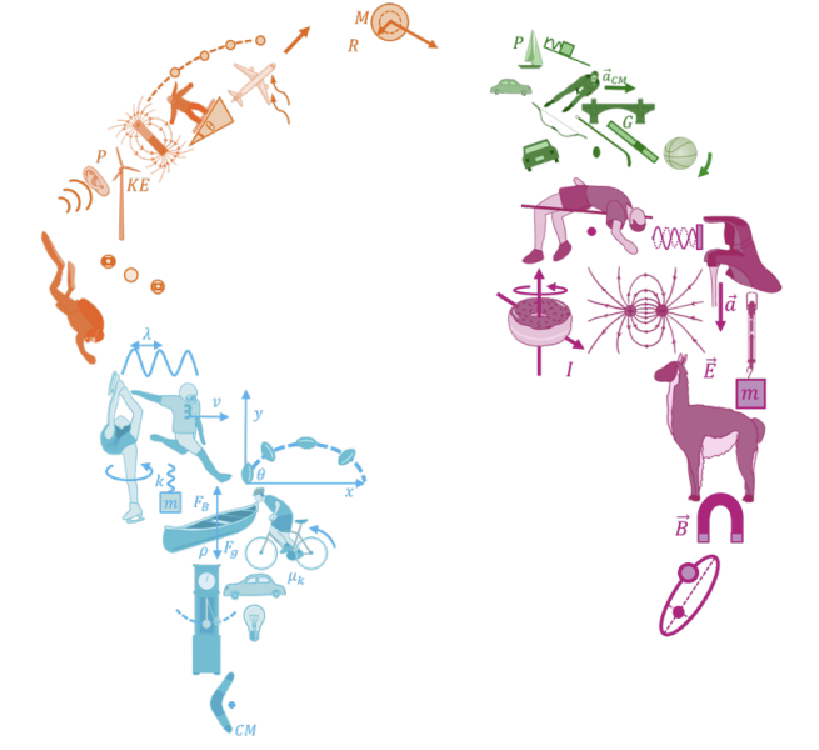
\includegraphics[width=4cm]{figures/BMDW/logo}
\end{textblock*}

\end{frame}

%%%%%%%%%%%%%TOC
\twocolframe{Outline}
  {\tableofcontents[sections={61}, subsectionstyle=show/show]\thispagestyle{empty}}
  {\tableofcontents[sections={62,63}, subsectionstyle=show/show]}
%%%%%%%%%%%%%%%%%%%%%%%%%







%%%%%%%%%%%%%%%%%%%%%%%%%%%%%%%%
\section{Biot-Savart Law}
\label{sec:biorsavartlaw}
\title{Biot-Savart Law}


%%%%%%%%%%%%%%%%%%%%%%%%%
\begin{frame}
\titlepage
\thispagestyle{empty}
\end{frame}

%%%%%%%%%%%%%%%%%%%%%%%%%%




\subsection{Review: calculating the electric field}
\label{subsec:reviewcalulatingtheelectricfield}
\begin{frame}{Review: Calculating the electric field}

Three ways to determine the electric field:
\begin{enumerate}
\item Model a charge distribution as the sum of point charges, $dq$:
\begin{align*}
E = \int dE=\int k\frac{dq}{r^2}
\end{align*}
\item Exploit symmetry and use Gauss' Law:
\begin{align*}
\oint \vec E \cdot d\vec A= \frac{Q}{\epsilon_0}
\end{align*}
\item Build from common charge distributions (e.g. model a plane as many lines of charge):
\begin{align*}
E=\frac{\lambda}{2\pi\epsilon_0 r}
\end{align*}
\end{enumerate}
\end{frame}

%%%%%%%%%%%%%%%%%%%%%%%%%%%%%%



%%%%%%%%%%%%%%%%%%%%%%%%%%%%%%
\subsection{Formula}
\label{subsec:bsformula}
\twocolframesf{The Biot-Savart Law}
{
A small section of wire, $d\vec l$, carrying current, $I$, will create a magnetic field, $d\vec B$, given by:
\begin{align*}
d\vec B = \frac{\mu_0I}{4\pi}\frac{d\vec l\times \hat r}{r^2}
\end{align*}
\begin{itemize}
\item $d\vec l$: the small segment (along wire, in direction of $I$).
\item $\vec r$: a vector \textbf{from the segment} to where we want to calculate the field.
\item $r$: the magnitude of $\vec r$.
\item $\hat r$: unit vector in direction of $\vec r$.  
\end{itemize}
}
{
\centering
\begin{tikzpicture}[scale=1]

\coordinate (a) at (0.62,1);
\coordinate (b) at (3.73,2.5);
\coordinate (c) at (2,1.55);
\coordinate (P) at ($(c)+(70:2)$);
%\fill (c) circle(3pt);

\draw[line width=2] (0,0) [out=80, in=250] to (4,3);
\draw[-latex, line width=2] (a) -- +(0.1,0.1) node[above]{$I$};
\draw[-latex, line width=2] (b) -- +(0.1,0.1) node[below]{$I$};
\draw[-latex, line width=2, color=qred] (c) -- +(19:0.9) node[below]{$d\vec l$};

\draw[line width=0.8] ($(c)+(70:0.4)$) arc (70:21:0.4)node[midway,above=4pt, right=-3pt]{$\theta$};

\draw[-latex, line width=1.5, color=qblue] (c) -- (P)node[midway,left]{$\vec r$};

\node[left=10pt,above=-3pt] at (P) {$P$};
\node[color=qblue] at (P) {\Large $\odot$};
\node[right=3pt, color=qblue] at (P) {$d\vec B$};
\end{tikzpicture}
\captionof*{figure}{\textit{Using the Biot-Savart law to determine the magnetic field at point $P$ due to the wire carrying current, $I$.}}

}

%%%%%%%%%%%%%%%%%%%%%%%%%%%%%%



%%%%%%%%%%%%%%%%%%%%%%%%%%%%%%
\subsection{The unit vector}
\label{subsec:theunitvector}
\begin{frame}{The unit vector}
\begin{itemize}
\item In practice, it is not always convenient to first calculate a vector, $\vec r$, and then a unit vector in that direction. Can use $\vec r$  directly in the Biot-Savart law:
\begin{align*}
d\vec B = \frac{\mu_0I}{4\pi}\frac{d\vec l\times \textcolor{qred}{\hat r}}{r^{\textcolor{qred}{2}}}
=\frac{\mu_0I}{4\pi}\frac{d\vec l\times \textcolor{qred}{\frac{\vec r}{r}}}{r^{\textcolor{qred}{2}}}
 = \frac{\mu_0I}{4\pi}\frac{d\vec l\times \textcolor{qred}{\vec r}}{r^{\textcolor{qred}{3}}} 
\end{align*}
\end{itemize}
\end{frame}


%%%%%%%%%%%%%%%%%%%%%%%%%%%%%%
\subsection{Magnetic field from a finite straight wire}
\label{subsec:magneticfieldfromafinitestraightwire}
\twocolframesf{Magnetic field from a straight wire of length $L$}
{
\begin{enumerate}
\item<1-> Make a good diagram.
\item<2-> Choose $d\vec l$.
\item<3-> Determine $d\vec l \times \vec r$:
\only<3>{
}
\only<4>{
\begin{align*}
d\vec l \times \vec r &= (dl \hat y) \times (r\cos\theta\hat x-r\sin\theta\hat y)
\end{align*}
}
\only<5>{
\begin{align*}
d\vec l \times \vec r &= (dl \hat y) \times (r\cos\theta\hat x-r\sin\theta\hat y)\\
&=dlr\cos\theta (\hat y\times \hat x) - dlr\sin\theta(\hat y \times \hat y)
\end{align*}
}
\only<6>{
\begin{align*}
d\vec l \times \vec r &= (dl \hat y) \times (r\cos\theta\hat x-r\sin\theta\hat y)\\
&=dlr\cos\theta \cancelto{(-\hat z)}{(\hat y\times \hat x)} - dlr\sin\theta\cancelto{0}{(\hat y \times \hat y)}
\end{align*}
}
\only<7>{
\begin{align*}
d\vec l \times \vec r &= (dl \hat y) \times (r\cos\theta\hat x-r\sin\theta\hat y)\\
&=dlr\cos\theta \cancelto{(-\hat z)}{(\hat y\times \hat x)} - dlr\sin\theta\cancelto{0}{(\hat y \times \hat y)}\\
&=-dlr\cos\theta\hat z
\end{align*}
}
\only<8->{
\begin{align*}
d\vec l \times \vec r =-r\cos\theta dl \hat z
\end{align*}
}
\item<8-> Determine $d\vec B$:
\only<9->{
\begin{align*}
d\vec B = \frac{\mu_0I}{4\pi}\frac{d\vec l\times \vec r}{r^3} =-\frac{\mu_0I}{4\pi}\frac{\cos\theta}{r^2}dl\hat z
\end{align*}

}

\end{enumerate}
}
{
\vspace{-0.25cm}
\centering
\begin{tikzpicture}[scale=1]
\def\L{5}
\def\D{3}
\def\dl{0.75}

\coordinate (P) at (\D,0);
\coordinate (PL) at (0,0.25*\L);


%Set up:
\draw[line width =3] (0,-\L/2) -- (0,\L/2);
\fill (P) circle(2pt);
\node[above=10pt,right=2pt] at (P) {$P$}; 
\draw[-latex] (0,0) -- ($(P)+(1.5\D,0)$) node[below]{$x$};
\draw[-latex,line width =3] (0,-0.5*\L) -- (0,-0.25*\L) node[right]{$I$};
\draw[-latex] (0,-0.6*\L) -- (0,0.6*\L) node[left]{$y$};
\draw[latex-latex] (-0.15*\L,-0.5*\L) -- (-0.15*\L,0.5*\L) node[midway,left]{$L$};
\draw[latex-latex] (0,-0.02*\L) -- (\D,-0.02*\L) node[midway, below] {$D$};


%construction
\only<2->{
\draw[-latex,color=qred,line width =3] ($ (PL)+(0,-0.5*\dl) $) -- +(0,\dl)node[midway,left]{$d\vec l$};
\draw[-latex, line width=1.5pt] (PL) -- (P) node[midway,above]{$\vec r$};
\begin{scope}
\clip (PL) -- (P) -- (0,0) --(PL);
\draw ($(P)+(-0.4*\D,0)$) arc(180:90:0.4*\D);
\end{scope}
\node[above] at (0.5*\D,0) {$\theta$};
}
\only<9->{%dB
\node[right=-5pt,color=qblue!80] at (P) {\huge $\times$};
\node[right=3pt, below=3pt,color=qblue!80] at (P) {$d\vec B$};
}
\end{tikzpicture}
\captionof*{figure}{\textit{Using the Biot-Savart law to determine the magnetic field at point $P$ due to the wire carrying current, $I$.}}
}

%%%%%%%%%%%%%%%%%%%%%%%%%%%%%%
\twocolframesf{Magnetic field from a straight wire of length $L$}
{
\begin{enumerate}
\setcounter{enumi}{3}
\item<1-> Determine $d\vec B$:
\begin{align*}
d\vec B =-\frac{\mu_0I}{4\pi}\cos\theta\frac{1}{r^2}dl\hat z
\end{align*}
\item<1-> Need to choose variable of integration ($dy$, $d\theta$) to integrate.
\only<3-5>{
\begin{itemize}
\item[$\rightarrow$]Choose $d\theta$:
\only<4-5>{
\begin{align*}
r &= \frac{D}{\cos\theta}\quad&\rightarrow & \quad &\therefore\quad &\frac{1}{r^2}&=&\frac{\cos^2}{D^2}\\
l &= D\tan\theta\quad&\rightarrow&\quad &\therefore\quad&dl&=&\frac{D}{\cos^2\theta}d\theta\\
\end{align*}
}
\only<5>{
\vspace{-1cm}
\begin{align*}
\therefore d\vec B =-\frac{\mu_0I}{4\pi}\cos\theta \frac{\cos^2\theta}{D^2}\frac{D}{\cos^2\theta}d\theta\hat z = -\frac{\mu_0I}{4\pi}\frac{\cos\theta}{D}d\theta\hat z
\end{align*}
}
\end{itemize}
}
\end{enumerate}
}
{
\vspace{-0.25cm}
\centering
\begin{tikzpicture}[scale=1]
\def\L{5}
\def\D{3}
\def\dl{0.75}

\coordinate (P) at (\D,0);
\coordinate (PL) at (0,0.25*\L);


%Set up:
\draw[line width =3] (0,-\L/2) -- (0,\L/2);
\fill (P) circle(2pt);
\node[above=10pt,right=2pt] at (P) {$P$}; 
\draw[-latex] (0,0) -- ($(P)+(1.5\D,0)$) node[below]{$x$};
\draw[-latex,line width =3] (0,-0.5*\L) -- (0,-0.25*\L) node[right]{$I$};
\draw[-latex] (0,-0.6*\L) -- (0,0.6*\L) node[left]{$y$};
\draw[latex-latex] (-0.15*\L,-0.5*\L) -- (-0.15*\L,0.5*\L) node[midway,left]{$L$};
\draw[latex-latex] (0,-0.02*\L) -- (\D,-0.02*\L) node[midway, below] {$D$};

\draw[-latex,color=qred,line width =3] ($ (PL)+(0,-0.5*\dl) $) -- +(0,\dl)node[midway,left]{$d\vec l$};
\draw[-latex, line width=1.5pt] (PL) -- (P) node[midway,above]{$\vec r$};
\begin{scope}
\clip (PL) -- (P) -- (0,0) --(PL);
\draw ($(P)+(-0.4*\D,0)$) arc(180:90:0.4*\D);
\end{scope}
\node[above] at (0.5*\D,0) {$\theta$};

\node[right=-5pt,color=qblue!80] at (P) {\huge $\times$};
\node[right=3pt, below=3pt,color=qblue!80] at (P) {$d\vec B$};

\end{tikzpicture}
\captionof*{figure}{\textit{Using the Biot-Savart law to determine the magnetic field at point $P$ due to the wire carrying current, $I$.}}
}


%%%%%%%%%%%%%%%%%%%%%%%%%%%%%%
\twocolframesf{Magnetic field from a straight wire of length $L$}
{
\begin{enumerate}
\setcounter{enumi}{5}
\item<1-> Do the integral:
\only<1>{
\begin{align*}
\vec B &= \int d\vec B =-\frac{\mu_0I}{4\pi D}\int_{\textcolor{qred}{-\theta_0}}^{\textcolor{qred}{+\theta_0}}\cos\theta d\theta\hat z
\end{align*}
}
\only<2>{
\begin{align*}
\vec B &= \int d\vec B =-\frac{\mu_0I}{4\pi D}\int_{\textcolor{qred}{-\theta_0}}^{\textcolor{qred}{+\theta_0}}\cos\theta d\theta\hat z\\
&=-\frac{\mu_0I}{4\pi D}\left[\sin\theta\right]_{-\theta_0}^{\theta_0}\hat z=-\frac{\mu_0I}{2\pi D}\sin\theta_0\hat z
\end{align*}
}
\only<3>{
\begin{align*}
\vec B &= \int d\vec B =-\frac{\mu_0I}{4\pi D}\int_{\textcolor{qred}{-\theta_0}}^{\textcolor{qred}{+\theta_0}}\cos\theta d\theta\hat z\\
&=-\frac{\mu_0I}{4\pi D}\left[\sin\theta\right]_{-\theta_0}^{\theta_0}\hat z=-\frac{\mu_0I}{2\pi D}\sin\theta_0\hat z\\
\therefore \vec B&=-\frac{\mu_0I}{2\pi D} \frac{L/2}{\sqrt{\left(L/2\right)^2+D^2}}{}  \hat z\\
\end{align*}
}
\end{enumerate}
}
{
\vspace{-0.25cm}
\centering
\begin{tikzpicture}[scale=1]
\def\L{5}
\def\D{3}
\def\dl{0.75}

\coordinate (P) at (\D,0);
\coordinate (PL) at (0,0.25*\L);


%Set up:
\draw[line width =3] (0,-\L/2) -- (0,\L/2);
\fill (P) circle(2pt);
\node[above=10pt,right=2pt] at (P) {$P$}; 
\draw[-latex] (0,0) -- ($(P)+(1.5\D,0)$) node[below]{$x$};
\draw[-latex,line width =3] (0,-0.5*\L) -- (0,-0.25*\L) node[right]{$I$};
\draw[-latex] (0,-0.6*\L) -- (0,0.6*\L) node[left]{$y$};
\draw[latex-latex] (-0.15*\L,-0.5*\L) -- (-0.15*\L,0.5*\L) node[midway,left]{$L$};
\draw[latex-latex] (0,-0.02*\L) -- (\D,-0.02*\L) node[midway, below] {$D$};

\draw[-latex,color=qred,line width =3] ($ (PL)+(0,-0.5*\dl) $) -- +(0,\dl)node[midway,left]{$d\vec l$};
\draw[-latex, line width=1.5pt] (PL) -- (P) node[midway,above]{$\vec r$};
\begin{scope}
\clip (PL) -- (P) -- (0,0) --(PL);
\draw ($(P)+(-0.4*\D,0)$) arc(180:90:0.4*\D);
\end{scope}
\node[above] at (0.5*\D,0) {$\theta$};

\node[right=-5pt,color=qblue!80] at (P) {\huge $\times$};
\node[right=3pt, below=3pt,color=qblue!80] at (P) {$d\vec B$};

%theta_0
\draw[line width =2pt,color=qred] (P) -- (0,-\L/2);
\begin{scope}
\clip (0,-\L/2)-- (P) -- (0,0) --(0,-\L/2);
\draw[line width =2pt,color=qred] ($(P)+(-0.35*\D,0)$) arc(180:270:0.35*\D);
\end{scope}
\node[below=-3pt,color=qred] at (0.76*\D,0) {\Large $\theta_0$};

\end{tikzpicture}
\captionof*{figure}{\textit{Using the Biot-Savart law to determine the magnetic field at point $P$ due to the wire carrying current, $I$.}}
}

%%%%%%%%%%%%%%%%%%%%%%%%%%%%%%




%%%%%%%%%%%%%%%%%%%%%%%%%%%%%%
\subsection{Magnetic field from an infinitely-long wire}
\label{subsec:magneticfieldfromaninfinitelylongwire}
\twocolframesf{Magnetic field from an infinitely-long wire}
{
\capfig{0.25}{figures/Bsource/axishand}{Right hand rule for axial vectors, used with thumb parallel to current.}
\begin{itemize}
\item The field lines are concentric with the wire (right hand rule for axial vectors).
\item The magnitude of the field at point, $P$, a distance, $r$, from the wire is:
\begin{align*}
B=\frac{\mu_0 I}{2\pi r}
\end{align*}
\end{itemize}
}
{
\centering
\begin{tikzpicture}[scale=1]
\def\L{5}
\def\D{1}

\draw[line width =3] (0,-\L/2) -- (0,\L/2);

\draw[color=qblue!80] (0,0) circle [x radius=0.5*\D, y radius=0.5*\D/4];
\draw[-latex, color=qblue!80] (0.5*\D,0) arc(0:60:{0.5*\D} and {0.5*\D/4});
\draw[color=qblue!80] (0,0) circle [x radius=\D, y radius=\D/4];
\draw[-latex, color=qblue!80] (1.0*\D,0) arc(0:60:{1.0*\D} and {1.0*\D/4});
\draw[color=qblue!80] (0,0) circle [x radius=1.5*\D, y radius=1.5*\D/4];
\draw[-latex, color=qblue!80] (1.5*\D,0) arc(0:60:{1.5*\D} and {1.5*\D/4});
\node[right, color=qblue!80] at (1.5*\D,0) {$\vec B$};
\draw[dashed] (0,0) -- (-1.5*\D,0) node[midway,above=7pt] {$r$};
\fill (-1.5*\D,0) circle(2pt);
\node[left] at (-1.5*\D,0) {$P$};
\draw[-latex,line width =3] (0,0) -- (0,0.3*\L) node[right]{$I$};

\end{tikzpicture}
\captionof*{figure}{\textit{Magnetic field forms concentric circles around the wire.}}
}

%%%%%%%%%%%%%%%%%%%%%%%%%%%%%%
\begin{bulletframe}{Force between 2 wires}
\item A wire carrying current produces a magnetic field:
\begin{align*}
B=\frac{\mu_0 I}{2\pi r}
\end{align*}
\item A wire carrying current in a magnetic field feels a force:
\begin{align*}
\vec F = I \vec l \times \vec B
\end{align*}
\item[$\rightarrow$] Two wires next to each other both carrying current must exert forces on each other!
\end{bulletframe}

%%%%%%%%%%%%%%%%%%%%%%%%%%%%%%



%%%%%%%%%%%%%%%%%%%%%%%%%%%%%%


%%%%%%%%%%%%%%%%%%%%%%%%%%%%%%
\subsection{Force between two wires}
\label{subsec:forcebetweentwowires}
\twocolframesf{Force between two wires}
{
\begin{itemize}
\item The field from wire 1:
\begin{align*}
B_1=\frac{\mu_0 I_1}{2\pi d}
\end{align*}
\item <2->The force on wire 2:
\begin{align*}
F_2 = I_2 L B_1 = \frac{\mu_0 I_1I_2 L}{2\pi d}
\end{align*}
\item<3-> Is the force on wire 1 from wire 2 the same?
\item<4->[$\rightarrow$] Newton's Third Law...
\end{itemize}
}
{
\centering
\begin{tikzpicture}[scale=1]
\def\L{5}
\def\D{2}

\draw[line width =3] (-\D/2,-\L/2) -- (-\D/2,\L/2);
\draw[line width =3] (\D/2,-\L/2) -- (\D/2,\L/2);
\draw[-latex,line width =3] (-\D/2,0) -- (-\D/2,0.3*\L) node[right]{$I_1$};
\draw[-latex,line width =3] (\D/2,0) -- (\D/2,0.3*\L) node[right]{$I_2$};


\draw[color=qblue!80] (-\D/2,0) circle [x radius=\D, y radius=\D/4];
\draw[-latex, color=qblue!80] (1.0*\D-\D/2,0) arc(0:60:{1.0*\D} and {1.0*\D/4}) node [above] {$\vec  B_1$};
\draw[latex-latex] (-\D/2,-0.25*\L) -- (\D/2,-0.25*\L) node[midway,below] {$d$} ;
%force vectors
\only<2->{
\draw[-latex,color=qred, line width =1.5pt] (\D/2,0) -- (0,0) node[below]{$\vec F$};
}
\only<4->{
\draw[color=qblue!80] (\D/2,0) circle [x radius=\D, y radius=\D/4];
\draw[-latex, color=qblue!80] (1.0*\D+\D/2,0) arc(0:60:{1.0*\D} and {1.0*\D/4}) node [above] {$\vec  B_2$};

\draw[-latex,color=qred, line width =1.5pt] (-\D/2,0) -- (0,0);
}
\end{tikzpicture}
\captionof*{figure}{\textit{Force between two wires}}
}



%%%%%%%%%%%%%%%%%%%%%%%%







%%%%%%%%%%%%%%%%%%%%%%%%




%%%%%%%%%%%%%%%%%%%%%%%%%%%%%%



%%%%%%%%%%%%%%%%%%%%%%%%%%%%%%
\twocolframesf{Field from a loop}
{
\begin{itemize}
\item Think of each section of the wire as a small straight wire.
\item The field looks like that from a bar magnet.
\end{itemize}
\begin{center}

\begin{tikzpicture}[scale=0.7]
\def\R{2}
\def\Rt{\R/3}
\def\sc{0.5}
\def\D{0.6}

%straight wire (like a sub figure)
\begin{scope}[scale=\sc,rotate=0,shift={(-3*\R,0)}]
\def\L{7}
\def\D{1.8}
\draw[line width =1.5pt] (0,-\L/2) -- (0,\L/2);
\draw[color=qblue!80] (0,0) circle [x radius=0.5*\D, y radius=0.5*\D/4];
\draw[-latex, color=qblue!80] (0.5*\D,0) arc(0:60:{0.5*\D} and {0.5*\D/4});
\draw[color=qblue!80] (0,0) circle [x radius=\D, y radius=\D/4];
\draw[-latex, color=qblue!80] (1.0*\D,0) arc(0:60:{1.0*\D} and {1.0*\D/4});
\draw[color=qblue!80] (0,0) circle [x radius=1.5*\D, y radius=1.5*\D/4];
\draw[-latex, color=qblue!80] (1.5*\D,0) arc(0:60:{1.5*\D} and {1.5*\D/4});
\draw[-latex,line width =1.5] (0,0) -- (0,0.3*\L) node[right]{$I$};
\end{scope}

%big loop
\draw[line width =2pt] (0,-\R) arc(270:90:{\Rt} and {\R});
\draw[line width =1pt, dashed] (0,-\R) arc(-90:90:{\Rt} and {\R});
\draw[line width =2pt,-latex] (-\Rt,0) arc(180:135:{\Rt} and \R) node[left] {$I$};
%fields
%fields around big loop
\begin{scope}[scale=1,rotate=0,shift={(-\Rt,0)}]
\draw[color=qblue!80] (0,0) circle [x radius=0.5*\D, y radius=0.5*\D/4];
\draw[-latex, color=qblue!80] (0.5*\D,0) arc(0:60:{0.5*\D} and {0.5*\D/4});
\draw[color=qblue!80] (0,0) circle [x radius=\D, y radius=\D/4];
\draw[-latex, color=qblue!80] (1.0*\D,0) arc(0:60:{1.0*\D} and {1.0*\D/4});
%\draw[color=qblue!80] (0,0) circle [x radius=1.5*\D, y radius=1.5*\D/4];
%\draw[-latex, color=qblue!80] (1.5*\D,0) arc(0:60:{1.5*\D} and {1.5*\D/4});
\end{scope}

\begin{scope}[scale=1,shift={(\Rt,0)}]
\draw[color=qblue!80] (0,0) circle [x radius=0.5*\D, y radius=0.5*\D/4];
\draw[-latex, color=qblue!80] (0.5*\D,0) arc(0:-140:{0.5*\D} and {0.5*\D/4});
\draw[color=qblue!80] (0,0) circle [x radius=\D, y radius=\D/4];
\draw[-latex, color=qblue!80] (1.0*\D,0) arc(0:-140:{1.0*\D} and {1.0*\D/4});
%\draw[color=qblue!80] (0,0) circle [x radius=1.5*\D, y radius=1.5*\D/4];
%\draw[-latex, color=qblue!80] (1.5*\D,0) arc(0:60:{1.5*\D} and {1.5*\D/4});
\end{scope}

\begin{scope}[scale=1,shift={(0,\R)}]
\draw[color=qblue!80] (0,0) circle (0.5*\D);
\draw[-latex, color=qblue!80] (0.5*\D,0) arc(0:-160:{0.5*\D} and {0.5*\D});
\draw[color=qblue!80] (0,0) circle (\D);
\draw[-latex, color=qblue!80] (1.0*\D,0) arc(0:-160:{1.0*\D} and {1.0*\D});
\end{scope}

\begin{scope}[scale=1,shift={(0,-\R)}]
\draw[color=qblue!80] (0,0) circle (0.5*\D);
\draw[latex-, color=qblue!80] (0.5*\D,0) arc(0:-140:{0.5*\D} and {0.5*\D});
\draw[color=qblue!80] (0,0) circle (\D);
\draw[latex-, color=qblue!80] (1.0*\D,0) arc(0:-140:{1.0*\D} and {1.0*\D});
\end{scope}

\end{tikzpicture}
\captionof*{figure}{\textit{From the magnetic field of a straight wire to that of a circular loop. }}

\end{center}
}
{
%\vspace{-1cm}

%\vspace{-0.5cm}
\capfig{1}{figures/Bsource/ring}{Magnetic field from a ring of current is the same as that of a dipole}.

}




%%%%%%%%%%%%%%%%%%%%%%%%%%%%%%



%%%%%%%%%%%%%%%%%%%%%%%%%%%%%%
%%%%%%%%%%% The ring
\subsection{Magnetic field from a ring of current}
\label{subsec:magneticfieldfromaringofcurrent}
\twocolframesf{Magnetic field from a ring of current}
{
\begin{enumerate}
\item<1-> Make a good diagram.
\item<2-> Choose $d\vec l$.
\item<3-> Determine $d \vec l\times \vec r$ : \only<5->{$\rightarrow$ magnitude  $=dl r$.}
\only<4>{
\begin{align*}
d\vec l \times \vec r &=(-dl \hat z) \times (r\cos\theta\hat x-r\sin\theta\hat y)\\
&=-dl r\cos\theta(\hat z \times \hat x) + dl r \sin\theta (\hat z \times \hat y)\\
&=-dl r\cos\theta(\hat y) - dl r \sin\theta (\hat x )
\end{align*}
}
\item<5-> Determine $d\vec B$ : \only<6->{$\rightarrow$ magnitude $=\frac{\mu_0Idl}{4\pi r^2}$.}
\only<5>{
\begin{align*}
d\vec B &= \frac{\mu_0I}{4\pi}\frac{d\vec l\times \vec r}{r^3} = -\frac{\mu_0Idl}{4\pi r^2}(\cos\theta(\hat y) + \sin\theta (\hat x ))
\end{align*}
}
\item<6-> Think about symmetry:
\end{enumerate}
}
{
\centering
\begin{tikzpicture}[scale=1]

\tikzmath{
\R = 1.75;
\L = 3;
\xp = 2;
\dl = 1.3; 
\dBs = 0.4;
\pa = 0; %phi, position of dl
\dlpx = 0;
\dlpy = cos(\pa)*\R;
\dlpz = sin(\pa)*\R;
%components of dl
\dlx = 0;
\dly = \dl*sin(\pa);
\dlz = -\dl*cos(\pa);
%cone opening angle
\th = atan(\R/\xp);
%r vector for cross-product
\rx = \xp;
\ry = -\dlpy;
\rz = -\dlpz;
\dBx = \dBs*(\dly*\rz-\dlz*\ry);
\dBy = \dBs*(\dlz*\rx-\dlx*\rz);
\dBz = \dBs*(\dlx*\ry-\dly*\rx);
\dBm = sqrt(\dBx*\dBx+\dBy*\dBy+\dBz*\dBz);
\dBr = \dBm*cos(\th);
\dBrx = \xp-\dBm*sin(\th);
}

\coordinate (P) at (\xp,0,0);
\coordinate (PL) at (\dlpx,\dlpy,\dlpz);

%axes:
\draw[-latex] (0,0,0) -- (\L,0,0) node[below] {$x$};
\draw[-latex] (0,0,0) -- (0,\L,0) node[left] {$y$};
\draw[-latex] (0,0,0) -- (0,0,\L) node[below] {$z$};
\draw[dashed] (0,0,0) -- (0,0,-\L);
\draw[dashed] (0,0,0) -- (0,-0.7*\L,0);
\draw[dashed] (0,0,0) -- (-0.4*\L,0,0);
%P
\node[below] at (P) {$P$};
\fill (P) circle(2pt);
%wire:
\begin{scope}[canvas is yz plane at x=0]
\draw[line width=3] (0,0) circle(\R);
\fill[opacity=0.05] (0,0) circle(\R);
\draw[line width=3,-latex] (140:\R) arc (140:110:\R) node[right] {$I$};
\end{scope}

\draw[latex-latex, dotted] (0,0,0) -- (0,\R,0) node[midway,right]{$R$};

%construction
\only<2->{
\begin{scope}[canvas is yz plane at x=0]
\draw[-latex,color=qred, line width = 2pt] (\dlpy,\dlpz) -- +(\dly,\dlz) node[above] {$d\vec l$};
\end{scope}

\draw[-latex, line width=1.5pt] (PL) -- (P) node[midway,above] {$\vec r$};
}

\only<3->{
%angle theta
\draw[color=qred,line width=2pt] (0.7*\xp,0) arc(180:180-\th:0.3*\xp) node[midway,left] {$\theta$};
}
\only<4>{
\draw[-latex, line width = 2pt] (P) -- +(\dBx,\dBy,\dBz) node[below] {$d\vec l\times \vec r$};
}

\only<5->{
\draw[-latex,color=qblue, line width = 2pt] (P) -- +(\dBx,\dBy,\dBz) node[below] {$d\vec B$};
}
\end{tikzpicture}
\captionof*{figure}{\textit{Using the Biot-Savart law to determine the magnetic field at point $P$ due to the ring carrying current, $I$.}}

}

%%%%%%%%%%%%%%%%%%%%%%%%%%%%%% phi = 0
\twocolframesf{Magnetic field from a ring of current}
{
\begin{enumerate}
\item Make a good diagram.
\item Choose $d\vec l$.
\item Determine $d \vec l\times \vec r$ : $\rightarrow$ magnitude  $=dl r$.
\item Determine $d\vec B$ : $\rightarrow$ magnitude $=\frac{\mu_0Idl}{4\pi r^2}$.
\item Think about symmetry:
\end{enumerate}
}
{
\centering
\begin{tikzpicture}[scale=1]

\tikzmath{
\R = 1.75;
\L = 3;
\xp = 2;
\dl = 1.3; 
\dBs = 0.4;
\pa = 0; %phi, position of dl
\dlpx = 0;
\dlpy = cos(\pa)*\R;
\dlpz = sin(\pa)*\R;
%components of dl
\dlx = 0;
\dly = \dl*sin(\pa);
\dlz = -\dl*cos(\pa);
%cone opening angle
\th = atan(\R/\xp);
%r vector for cross-product
\rx = \xp;
\ry = -\dlpy;
\rz = -\dlpz;
\dBx = \dBs*(\dly*\rz-\dlz*\ry);
\dBy = \dBs*(\dlz*\rx-\dlx*\rz);
\dBz = \dBs*(\dlx*\ry-\dly*\rx);
\dBm = sqrt(\dBx*\dBx+\dBy*\dBy+\dBz*\dBz);
\dBr = \dBm*cos(\th);
\dBrx = \xp-\dBm*sin(\th);
}

\coordinate (P) at (\xp,0,0);
\coordinate (PL) at (\dlpx,\dlpy,\dlpz);

%axes:
\draw[-latex] (0,0,0) -- (\L,0,0) node[below] {$x$};
\draw[-latex] (0,0,0) -- (0,\L,0) node[left] {$y$};
\draw[-latex] (0,0,0) -- (0,0,\L) node[below] {$z$};
\draw[dashed] (0,0,0) -- (0,0,-\L);
\draw[dashed] (0,0,0) -- (0,-0.7*\L,0);
\draw[dashed] (0,0,0) -- (-0.4*\L,0,0);
%P
\node[below] at (P) {$P$};
\fill (P) circle(2pt);
%wire:
\begin{scope}[canvas is yz plane at x=0]
\draw[line width=3] (0,0) circle(\R);
\fill[opacity=0.05] (0,0) circle(\R);
\draw[line width=3,-latex] (140:\R) arc (140:110:\R) node[right] {$I$};
\end{scope}

\draw[latex-latex, dotted] (0,0,0) -- (0,\R,0) node[midway,right]{$R$};


%construction
\begin{scope}[canvas is yz plane at x=0]
\draw[-latex,color=qred, line width = 2pt] (\dlpy,\dlpz) -- +(\dly,\dlz) node[above] {$d\vec l$};
\end{scope}

\draw[-latex, line width=1.5pt] (PL) -- (P) node[midway,above] {$\vec r$};

\draw[-latex,color=qblue, line width = 2pt] (P) -- +(\dBx,\dBy,\dBz) node[below] {$d\vec B$};

%angle theta
\draw[color=qred,line width=2pt] (0.7*\xp,0) arc(180:180-\th:0.3*\xp) node[midway,left] {$\theta$};


\end{tikzpicture}
\captionof*{figure}{\textit{Using the Biot-Savart law to determine the magnetic field at point $P$ due to the ring carrying current, $I$.}}
}

%%%%%%%%%%%%%%%%%%%%%%%%%%%%%%  phi=270
\twocolframesf{Magnetic field from a ring of current}
{
\begin{enumerate}
\item Make a good diagram.
\item Choose $d\vec l$.
\item Determine $d \vec l\times \vec r$ : $\rightarrow$ magnitude  $=dl r$.
\item Determine $d\vec B$ : $\rightarrow$ magnitude $=\frac{\mu_0Idl}{4\pi r^2}$.
\item Think about symmetry:
\end{enumerate}
}
{
\centering
\begin{tikzpicture}[scale=1]

\tikzmath{
\R = 1.75;
\L = 3;
\xp = 2;
\dl = 1.3; 
\dBs = 0.4;
\pa = 270; %phi, position of dl
\dlpx = 0;
\dlpy = cos(\pa)*\R;
\dlpz = sin(\pa)*\R;
%components of dl
\dlx = 0;
\dly = \dl*sin(\pa);
\dlz = -\dl*cos(\pa);
%cone opening angle
\th = atan(\R/\xp);
%r vector for cross-product
\rx = \xp;
\ry = -\dlpy;
\rz = -\dlpz;
\dBx = \dBs*(\dly*\rz-\dlz*\ry);
\dBy = \dBs*(\dlz*\rx-\dlx*\rz);
\dBz = \dBs*(\dlx*\ry-\dly*\rx);
\dBm = sqrt(\dBx*\dBx+\dBy*\dBy+\dBz*\dBz);
\dBr = \dBm*cos(\th);
\dBrx = \xp-\dBm*sin(\th);
}

\coordinate (P) at (\xp,0,0);
\coordinate (PL) at (\dlpx,\dlpy,\dlpz);

%axes:
\draw[-latex] (0,0,0) -- (\L,0,0) node[below] {$x$};
\draw[-latex] (0,0,0) -- (0,\L,0) node[left] {$y$};
\draw[-latex] (0,0,0) -- (0,0,\L) node[below] {$z$};
\draw[dashed] (0,0,0) -- (0,0,-\L);
\draw[dashed] (0,0,0) -- (0,-0.7*\L,0);
\draw[dashed] (0,0,0) -- (-0.4*\L,0,0);
%P
\node[below] at (P) {$P$};
\fill (P) circle(2pt);
%wire:
\begin{scope}[canvas is yz plane at x=0]
\draw[line width=3] (0,0) circle(\R);
\fill[opacity=0.05] (0,0) circle(\R);
\draw[line width=3,-latex] (140:\R) arc (140:110:\R) node[right] {$I$};
\end{scope}

\draw[latex-latex, dotted] (0,0,0) -- (0,\R,0) node[midway,right]{$R$};

%construction
\begin{scope}[canvas is yz plane at x=0]
\draw[-latex,color=qred, line width = 2pt] (\dlpy,\dlpz) -- +(\dly,\dlz) node[midway,left] {$d\vec l$};
\end{scope}

\draw[-latex, line width=1.5pt] (PL) -- (P) node[midway,above] {$\vec r$};

\draw[-latex,color=qblue, line width = 2pt] (P) -- +(\dBx,\dBy,\dBz) node[below] {$d\vec B$};

\end{tikzpicture}
\captionof*{figure}{\textit{Using the Biot-Savart law to determine the magnetic field at point $P$ due to the ring carrying current, $I$.}}

}

%%%%%%%%%%%%%%%%%%%%%%%%%%%%%% phi  180
\twocolframesf{Magnetic field from a ring of current}
{
\begin{enumerate}
\item Make a good diagram.
\item Choose $d\vec l$.
\item Determine $d \vec l\times \vec r$ : $\rightarrow$ magnitude  $=dl r$.
\item Determine $d\vec B$ : $\rightarrow$ magnitude $=\frac{\mu_0Idl}{4\pi r^2}$.
\item Think about symmetry:
\end{enumerate}
}
{
\centering
\begin{tikzpicture}[scale=1]

\tikzmath{
\R = 1.75;
\L = 3;
\xp = 2;
\dl = 1.3; 
\dBs = 0.4;
\pa = 180; %phi, position of dl
\dlpx = 0;
\dlpy = cos(\pa)*\R;
\dlpz = sin(\pa)*\R;
%components of dl
\dlx = 0;
\dly = \dl*sin(\pa);
\dlz = -\dl*cos(\pa);
%cone opening angle
\th = atan(\R/\xp);
%r vector for cross-product
\rx = \xp;
\ry = -\dlpy;
\rz = -\dlpz;
\dBx = \dBs*(\dly*\rz-\dlz*\ry);
\dBy = \dBs*(\dlz*\rx-\dlx*\rz);
\dBz = \dBs*(\dlx*\ry-\dly*\rx);
\dBm = sqrt(\dBx*\dBx+\dBy*\dBy+\dBz*\dBz);
\dBr = \dBm*cos(\th);
\dBrx = \xp-\dBm*sin(\th);
}

\coordinate (P) at (\xp,0,0);
\coordinate (PL) at (\dlpx,\dlpy,\dlpz);

%axes:
\draw[-latex] (0,0,0) -- (\L,0,0) node[below] {$x$};
\draw[-latex] (0,0,0) -- (0,\L,0) node[left] {$y$};
\draw[-latex] (0,0,0) -- (0,0,\L) node[below] {$z$};
\draw[dashed] (0,0,0) -- (0,0,-\L);
\draw[dashed] (0,0,0) -- (0,-0.7*\L,0);
\draw[dashed] (0,0,0) -- (-0.4*\L,0,0);
%P
\node[below] at (P) {$P$};
\fill (P) circle(2pt);
%wire:
\begin{scope}[canvas is yz plane at x=0]
\draw[line width=3] (0,0) circle(\R);
\fill[opacity=0.05] (0,0) circle(\R);
\draw[line width=3,-latex] (140:\R) arc (140:110:\R) node[right] {$I$};
\end{scope}

\draw[latex-latex, dotted] (0,0,0) -- (0,\R,0) node[midway,right]{$R$};

%construction
\begin{scope}[canvas is yz plane at x=0]
\draw[-latex,color=qred, line width = 2pt] (\dlpy,\dlpz) -- +(\dly,\dlz) node[below] {$d\vec l$};
\end{scope}

\draw[-latex, line width=1.5pt] (PL) -- (P) node[midway,above] {$\vec r$};

\draw[-latex,color=qblue, line width = 2pt] (P) -- +(\dBx,\dBy,\dBz) node[below] {$d\vec B$};

\end{tikzpicture}
\captionof*{figure}{\textit{Using the Biot-Savart law to determine the magnetic field at point $P$ due to the ring carrying current, $I$.}}
}

%%%%%%%%%%%%%%%%%%%%%%%%%%%%%% phi = 90
\twocolframesf{Magnetic field from a ring of current}
{
\begin{enumerate}
\item Make a good diagram.
\item Choose $d\vec l$.
\item Determine $d \vec l\times \vec r$ : $\rightarrow$ magnitude  $=dl r$.
\item Determine $d\vec B$ : $\rightarrow$ magnitude $=\frac{\mu_0Idl}{4\pi r^2}$.
\item Think about symmetry:
\end{enumerate}
}
{
\centering
\begin{tikzpicture}[scale=1]

\tikzmath{
\R = 1.75;
\L = 3;
\xp = 2;
\dl = 1.3; 
\dBs = 0.4;
\pa = 90; %phi, position of dl
\dlpx = 0;
\dlpy = cos(\pa)*\R;
\dlpz = sin(\pa)*\R;
%components of dl
\dlx = 0;
\dly = \dl*sin(\pa);
\dlz = -\dl*cos(\pa);
%cone opening angle
\th = atan(\R/\xp);
%r vector for cross-product
\rx = \xp;
\ry = -\dlpy;
\rz = -\dlpz;
\dBx = \dBs*(\dly*\rz-\dlz*\ry);
\dBy = \dBs*(\dlz*\rx-\dlx*\rz);
\dBz = \dBs*(\dlx*\ry-\dly*\rx);
\dBm = sqrt(\dBx*\dBx+\dBy*\dBy+\dBz*\dBz);
\dBr = \dBm*cos(\th);
\dBrx = \xp-\dBm*sin(\th);
}

\coordinate (P) at (\xp,0,0);
\coordinate (PL) at (\dlpx,\dlpy,\dlpz);

%axes:
\draw[-latex] (0,0,0) -- (\L,0,0) node[below] {$x$};
\draw[-latex] (0,0,0) -- (0,\L,0) node[left] {$y$};
\draw[-latex] (0,0,0) -- (0,0,\L) node[below] {$z$};
\draw[dashed] (0,0,0) -- (0,0,-\L);
\draw[dashed] (0,0,0) -- (0,-0.7*\L,0);
\draw[dashed] (0,0,0) -- (-0.4*\L,0,0);
%P
\node[below] at (P) {$P$};
\fill (P) circle(2pt);
%wire:
\begin{scope}[canvas is yz plane at x=0]
\draw[line width=3] (0,0) circle(\R);
\fill[opacity=0.05] (0,0) circle(\R);
\draw[line width=3,-latex] (140:\R) arc (140:110:\R) node[right] {$I$};
\end{scope}

\draw[latex-latex, dotted] (0,0,0) -- (0,\R,0) node[midway,right]{$R$};

%construction
\begin{scope}[canvas is yz plane at x=0]
\draw[-latex,color=qred, line width = 2pt] (\dlpy,\dlpz) -- +(\dly,\dlz) node[above] {$d\vec l$};
\end{scope}
\draw[-latex, line width=1.5pt] (PL) -- (P) node[midway,above] {$\vec r$};
\draw[-latex,color=qblue, line width = 2pt] (P) -- +(\dBx,\dBy,\dBz) node[below] {$d\vec B$};

\end{tikzpicture}
\captionof*{figure}{\textit{Using the Biot-Savart law to determine the magnetic field at point $P$ due to the ring carrying current, $I$.}}
}

%%%%%%%%%%%%%%%%%%%%%%%%%%%%%% with circle
\twocolframesf{Magnetic field from a ring of current}
{
\begin{enumerate}
\item Make a good diagram.
\item Choose $d\vec l$.
\item Determine $d \vec l\times \vec r$ : $\rightarrow$ magnitude  $=dl r$.
\item Determine $d\vec B$ : $\rightarrow$ magnitude $=\frac{\mu_0Idl}{4\pi r^2}$.
\item Think about symmetry:
\end{enumerate}
\emph{The tip of the magnetic field vector traces out a circle. Only the component along $-x$ will survive the integral. }
}
{
\centering
\begin{tikzpicture}[scale=1]

\tikzmath{
\R = 1.75;
\L = 3;
\xp = 2;
\dl = 1.3; 
\dBs = 0.4;
\pa = 0; %phi, position of dl
\dlpx = 0;
\dlpy = cos(\pa)*\R;
\dlpz = sin(\pa)*\R;
%components of dl
\dlx = 0;
\dly = \dl*sin(\pa);
\dlz = -\dl*cos(\pa);
%cone opening angle
\th = atan(\R/\xp);
%r vector for cross-product
\rx = \xp;
\ry = -\dlpy;
\rz = -\dlpz;
\dBx = \dBs*(\dly*\rz-\dlz*\ry);
\dBy = \dBs*(\dlz*\rx-\dlx*\rz);
\dBz = \dBs*(\dlx*\ry-\dly*\rx);
\dBm = sqrt(\dBx*\dBx+\dBy*\dBy+\dBz*\dBz);
\dBr = \dBm*cos(\th);
\dBrx = \xp-\dBm*sin(\th);
}

\coordinate (P) at (\xp,0,0);
\coordinate (PL) at (\dlpx,\dlpy,\dlpz);

%axes:
\draw[-latex] (0,0,0) -- (\L,0,0) node[below] {$x$};
\draw[-latex] (0,0,0) -- (0,\L,0) node[left] {$y$};
\draw[-latex] (0,0,0) -- (0,0,\L) node[below] {$z$};
\draw[dashed] (0,0,0) -- (0,0,-\L);
\draw[dashed] (0,0,0) -- (0,-0.7*\L,0);
\draw[dashed] (0,0,0) -- (-0.4*\L,0,0);
%P
\node[below] at (P) {$P$};
\fill (P) circle(2pt);
%wire:
\begin{scope}[canvas is yz plane at x=0]
\draw[line width=3] (0,0) circle(\R);
\fill[opacity=0.05] (0,0) circle(\R);
\draw[line width=3,-latex] (140:\R) arc (140:110:\R) node[right] {$I$};
\end{scope}

\draw[latex-latex, dotted] (0,0,0) -- (0,\R,0) node[midway,right]{$R$};

%construction
\begin{scope}[canvas is yz plane at x=0]
\draw[-latex,color=qred, line width = 2pt] (\dlpy,\dlpz) -- +(\dly,\dlz) node[above] {$d\vec l$};
\end{scope}

\draw[-latex, line width=1.5pt] (PL) -- (P) node[midway,above] {$\vec r$};

\draw[-latex,color=qblue, line width = 2pt] (P) -- +(\dBx,\dBy,\dBz) node[below] {$d\vec B$};
%circle for tip of B
\begin{scope}[canvas is yz plane at x=\dBrx]
\draw[color=qblue, line width = 0.75pt, dashed] (0,0) circle(\dBr);
\end{scope}

\end{tikzpicture}
\captionof*{figure}{\textit{Using the Biot-Savart law to determine the magnetic field at point $P$ due to the ring carrying current, $I$.}}

}

%%%%%%%%%%%%%%%%%%%%%%%%%%%%%%
%%%%%%%%%%%%%%%%%%%%%%%%%%%%%%%%%%%
%%%%%% animation
%%%%%%%%%%%%%%%%%%%%%%%%%%%%%%%%%%%
\begin{frame}
\centering
\pgfmathtruncatemacro\N{40}
\begin{animateinline}[controls,loop]{5} % 5 fps, same as 0.2 s transduration

\multiframe{\N}{i=0+1}{

\begin{tikzpicture}[scale=1]

\tikzmath{
\R = 1.75;
\L = 3;
\xp = 2;
\dl = 1.3; 
\dBs = 0.4;
\pa = -\i*360/\N; %phi, position of dl
\dlpx = 0;
\dlpy = cos(\pa)*\R;
\dlpz = sin(\pa)*\R;
%components of dl
\dlx = 0;
\dly = \dl*sin(\pa);
\dlz = -\dl*cos(\pa);
%cone opening angle
\th = atan(\R/\xp);
%r vector for cross-product
\rx = \xp;
\ry = -\dlpy;
\rz = -\dlpz;
\dBx = \dBs*(\dly*\rz-\dlz*\ry);
\dBy = \dBs*(\dlz*\rx-\dlx*\rz);
\dBz = \dBs*(\dlx*\ry-\dly*\rx);
\dBm = sqrt(\dBx*\dBx+\dBy*\dBy+\dBz*\dBz);
\dBr = \dBm*cos(\th);
\dBrx = \xp-\dBm*sin(\th);
}

\coordinate (P) at (\xp,0,0);
\coordinate (PL) at (\dlpx,\dlpy,\dlpz);

%axes:
\draw[-latex] (0,0,0) -- (\L,0,0) node[below] {$x$};
\draw[-latex] (0,0,0) -- (0,\L,0) node[left] {$y$};
\draw[-latex] (0,0,0) -- (0,0,\L) node[below] {$z$};
\draw[dashed] (0,0,0) -- (0,0,-\L);
\draw[dashed] (0,0,0) -- (0,-0.7*\L,0);
\draw[dashed] (0,0,0) -- (-0.4*\L,0,0);
%P
\node[below] at (P) {$P$};
\fill (P) circle(2pt);
%wire:
\begin{scope}[canvas is yz plane at x=0]
\draw[line width=3] (0,0) circle(\R);
\fill[opacity=0.05] (0,0) circle(\R);
\draw[line width=3,-latex] (140:\R) arc (140:110:\R) node[right] {$I$};
\end{scope}

%construction
\begin{scope}[canvas is yz plane at x=0]
\draw[-latex,color=qred, line width = 2pt] (\dlpy,\dlpz) -- +(\dly,\dlz) node[above] {$d\vec l$};
\end{scope}

\draw[latex-latex, dotted] (0,0,0) -- (0,\R,0) node[midway,right]{$R$};

\draw[-latex, line width=1.5pt] (PL) -- (P) node[midway,above] {$\vec r$};

\draw[-latex,color=qblue, line width = 2pt] (P) -- +(\dBx,\dBy,\dBz) node[below] {$d\vec B$};
%circle for tip of B
\begin{scope}[canvas is yz plane at x=\dBrx]
\draw[color=qblue, line width = 0.75pt, dashed] (0,0) circle(\dBr);
\end{scope}

\end{tikzpicture}

}
\end{animateinline}
\end{frame}


%%%%%%%%%%%%%%%%%%%%%%%%%%%%%% with circle

\twocolframesf{Magnetic field from a ring of current}
{
\begin{enumerate}
\item Make a good diagram.
\item Choose $d\vec l$.
\item Determine $d \vec l\times \vec r$ : $\rightarrow$ magnitude  $=dl r$.
\item Determine $d\vec B$ : $\rightarrow$ magnitude $=\frac{\mu_0Idl}{4\pi r^2}$.
\item Think about symmetry:
\end{enumerate}
Only the $x$ component of the $d\vec B$ don't cancel out:
\only<1>{
\begin{align*}
dB_x=dB\cos\dots
\end{align*}
}
\only<2>{
\begin{align*}
dB_x=dB\cos\left(\frac{\pi}{2}-\theta\right)=dB\sin\theta
\end{align*}
}
}
{
\centering
\begin{tikzpicture}[scale=1]

\tikzmath{
\R = 1.75;
\L = 3;
\xp = 2;
\dl = 1.3; 
\dBs = 0.4;
\pa = 0; %phi, position of dl
\dlpx = 0;
\dlpy = cos(\pa)*\R;
\dlpz = sin(\pa)*\R;
%components of dl
\dlx = 0;
\dly = \dl*sin(\pa);
\dlz = -\dl*cos(\pa);
%cone opening angle
\th = atan(\R/\xp);
%r vector for cross-product
\rx = \xp;
\ry = -\dlpy;
\rz = -\dlpz;
\dBx = \dBs*(\dly*\rz-\dlz*\ry);
\dBy = \dBs*(\dlz*\rx-\dlx*\rz);
\dBz = \dBs*(\dlx*\ry-\dly*\rx);
\dBm = sqrt(\dBx*\dBx+\dBy*\dBy+\dBz*\dBz);
\dBr = \dBm*cos(\th);
\dBrx = \xp-\dBm*sin(\th);
}

\coordinate (P) at (\xp,0,0);
\coordinate (PL) at (\dlpx,\dlpy,\dlpz);

%axes:
\draw[-latex] (0,0,0) -- (\L,0,0) node[below] {$x$};
\draw[-latex] (0,0,0) -- (0,\L,0) node[left] {$y$};
\draw[-latex] (0,0,0) -- (0,0,\L) node[below] {$z$};
\draw[dashed] (0,0,0) -- (0,0,-\L);
\draw[dashed] (0,0,0) -- (0,-0.7*\L,0);
\draw[dashed] (0,0,0) -- (-0.4*\L,0,0);
%P
\node[below] at (P) {$P$};
\fill (P) circle(2pt);
%wire:
\begin{scope}[canvas is yz plane at x=0]
\draw[line width=3] (0,0) circle(\R);
\fill[opacity=0.05] (0,0) circle(\R);
\draw[line width=3,-latex] (140:\R) arc (140:110:\R) node[right] {$I$};
\end{scope}

%construction
\begin{scope}[canvas is yz plane at x=0]
\draw[-latex,color=qred, line width = 2pt] (\dlpy,\dlpz) -- +(\dly,\dlz) node[above] {$d\vec l$};
\end{scope}
\draw[latex-latex, dotted] (0,0,0) -- (0,\R,0) node[midway,right]{$R$};

\draw[-latex, line width=1.5pt] (PL) -- (P) node[midway,above] {$\vec r$};

\draw[-latex,color=qblue, line width = 2pt] (P) -- +(\dBx,\dBy,\dBz) node[below] {$d\vec B$};
%circle for tip of B
\begin{scope}[canvas is yz plane at x=\dBrx]
\draw[color=qblue, line width = 0.75pt, dashed] (0,0) circle(\dBr);
\end{scope}

%angle theta
\draw[color=qred,line width=2pt] (0.7*\xp,0) arc(180:180-\th:0.3*\xp) node[midway,left] {$\theta$};
%angle  90 -theta
\only<2>{
\draw[color=qblue,line width=2pt] (0.7*\xp,0) arc(180:180+90-\th:0.3*\xp) node[fill=white,midway,left=5pt] {$\frac{\pi}{2}-\theta$};
}

\end{tikzpicture}
\captionof*{figure}{\textit{Using the Biot-Savart law to determine the magnetic field at point $P$ due to the ring carrying current, $I$.}}

}


%%%%%%%%%%%%%%%%%%%%%%%%%%%%%% Finally

\twocolframesf{Magnetic field from a ring of current}
{
\begin{enumerate}
\item Make a good diagram.
\item Choose $d\vec l$.
\item Determine $d \vec l\times \vec r$ : $\rightarrow$ magnitude  $=dl r$.
\item Determine $d\vec B$ : $\rightarrow$ magnitude $=\frac{\mu_0Idl}{4\pi r^2}$.
\item Think about symmetry: $dB_x=dB\sin\theta$
\end{enumerate}
All together:
\begin{align*}
B_x = \int dB_x = \int dB\sin\theta =  \frac{\mu_0I}{4\pi}\int \frac{1}{r^2}\sin\theta dl
\end{align*}
\only<3>{
\begin{align*}
= \frac{\mu_0I}{4\pi r^2}\sin\theta  \int_0^{2\pi R} dl = \frac{\mu_0I}{4\pi r^2}\sin\theta (2\pi R)
\end{align*}
}
}
{
\centering
\begin{tikzpicture}[scale=1]

\tikzmath{
\R = 1.75;
\L = 3;
\xp = 2;
\dl = 1.3; 
\dBs = 0.4;
\pa = 0; %phi, position of dl
\dlpx = 0;
\dlpy = cos(\pa)*\R;
\dlpz = sin(\pa)*\R;
%components of dl
\dlx = 0;
\dly = \dl*sin(\pa);
\dlz = -\dl*cos(\pa);
%cone opening angle
\th = atan(\R/\xp);
%r vector for cross-product
\rx = \xp;
\ry = -\dlpy;
\rz = -\dlpz;
\dBx = \dBs*(\dly*\rz-\dlz*\ry);
\dBy = \dBs*(\dlz*\rx-\dlx*\rz);
\dBz = \dBs*(\dlx*\ry-\dly*\rx);
\dBm = sqrt(\dBx*\dBx+\dBy*\dBy+\dBz*\dBz);
\dBr = \dBm*cos(\th);
\dBrx = \xp-\dBm*sin(\th);
}

\coordinate (P) at (\xp,0,0);
\coordinate (PL) at (\dlpx,\dlpy,\dlpz);

%axes:
\draw[-latex] (0,0,0) -- (\L,0,0) node[below] {$x$};
\draw[-latex] (0,0,0) -- (0,\L,0) node[left] {$y$};
\draw[-latex] (0,0,0) -- (0,0,\L) node[below] {$z$};
\draw[dashed] (0,0,0) -- (0,0,-\L);
\draw[dashed] (0,0,0) -- (0,-0.7*\L,0);
\draw[dashed] (0,0,0) -- (-0.4*\L,0,0);
%P
\node[below] at (P) {$P$};
\fill (P) circle(2pt);
%wire:
\begin{scope}[canvas is yz plane at x=0]
\draw[line width=3] (0,0) circle(\R);
\fill[opacity=0.05] (0,0) circle(\R);
\draw[line width=3,-latex] (140:\R) arc (140:110:\R) node[right] {$I$};
\end{scope}

%construction
\begin{scope}[canvas is yz plane at x=0]
\draw[-latex,color=qred, line width = 2pt] (\dlpy,\dlpz) -- +(\dly,\dlz) node[above] {$d\vec l$};
\end{scope}

\draw[latex-latex, dotted] (0,0,0) -- (0,\R,0) node[midway,right]{$R$};

\draw[-latex, line width=1.5pt] (PL) -- (P) node[midway,above] {$\vec r$};

\draw[-latex,color=qblue, line width = 2pt] (P) -- +(\dBx,\dBy,\dBz) node[below] {$d\vec B$};
%circle for tip of B
\begin{scope}[canvas is yz plane at x=\dBrx]
\draw[color=qblue, line width = 0.75pt, dashed] (0,0) circle(\dBr);
\end{scope}

%angle theta
\draw[color=qred,line width=2pt] (0.7*\xp,0) arc(180:180-\th:0.3*\xp) node[midway,left] {$\theta$};
%angle  90 -theta

\end{tikzpicture}
\captionof*{figure}{\textit{Using the Biot-Savart law to determine the magnetic field at point $P$ due to the ring carrying current, $I$.}}

}


%%%%%%%%%%%%%%%%%%%%%%%%%%%%%% Finally

\twocolframesf{Magnetic field from a ring of current}
{
And, finally, with $P$ located a distance $x$ from the origin:
\begin{align*}
B_x &= -\frac{\mu_0I}{4\pi r^2}\sin\theta (2\pi R)\\
r &= \sqrt{R^2+x^2}\\
\sin\theta&=\frac{R}{r}=\frac{R}{\sqrt{R^2+x^2}}
\end{align*}
\begin{align*}
\boxed{\vec B = -\frac{\mu_0I}{2}\frac{R^2}{(R^2+x^2)^{\frac{3}{2}}} \hat x}
\end{align*}
}
{
\centering
\begin{tikzpicture}[scale=1]

\tikzmath{
\R = 1.75;
\L = 3;
\xp = 2;
\dl = 1.3; 
\dBs = 0.4;
\pa = 0; %phi, position of dl
\dlpx = 0;
\dlpy = cos(\pa)*\R;
\dlpz = sin(\pa)*\R;
%components of dl
\dlx = 0;
\dly = \dl*sin(\pa);
\dlz = -\dl*cos(\pa);
%cone opening angle
\th = atan(\R/\xp);
%r vector for cross-product
\rx = \xp;
\ry = -\dlpy;
\rz = -\dlpz;
\dBx = \dBs*(\dly*\rz-\dlz*\ry);
\dBy = \dBs*(\dlz*\rx-\dlx*\rz);
\dBz = \dBs*(\dlx*\ry-\dly*\rx);
\dBm = sqrt(\dBx*\dBx+\dBy*\dBy+\dBz*\dBz);
\dBr = \dBm*cos(\th);
\dBrx = \xp-\dBm*sin(\th);
}

\coordinate (P) at (\xp,0,0);
\coordinate (PL) at (\dlpx,\dlpy,\dlpz);

%axes:
\draw[-latex] (0,0,0) -- (\L,0,0) node[below] {$x$};
\draw[-latex] (0,0,0) -- (0,\L,0) node[left] {$y$};
\draw[-latex] (0,0,0) -- (0,0,\L) node[below] {$z$};
\draw[dashed] (0,0,0) -- (0,0,-\L);
\draw[dashed] (0,0,0) -- (0,-0.7*\L,0);
\draw[dashed] (0,0,0) -- (-0.4*\L,0,0);
%P
\node[below] at (P) {$P$};
\fill (P) circle(2pt);
%wire:
\begin{scope}[canvas is yz plane at x=0]
\draw[line width=3] (0,0) circle(\R);
\fill[opacity=0.05] (0,0) circle(\R);
\draw[line width=3,-latex] (140:\R) arc (140:110:\R) node[right] {$I$};
\end{scope}

%construction
\begin{scope}[canvas is yz plane at x=0]
\draw[-latex,color=qred, line width = 2pt] (\dlpy,\dlpz) -- +(\dly,\dlz) node[above] {$d\vec l$};
\end{scope}

\draw[latex-latex, dotted] (0,0,0) -- (0,\R,0) node[midway,right]{$R$};

\draw[-latex, line width=1.5pt] (PL) -- (P) node[midway,above] {$\vec r$};

\draw[-latex,color=qblue, line width = 2pt] (P) -- +(\dBx,\dBy,\dBz) node[below] {$d\vec B$};
%circle for tip of B
\begin{scope}[canvas is yz plane at x=\dBrx]
\draw[color=qblue, line width = 0.75pt, dashed] (0,0) circle(\dBr);
\end{scope}

%angle theta
\draw[color=qred,line width=2pt] (0.7*\xp,0) arc(180:180-\th:0.3*\xp) node[midway,left] {$\theta$};
%angle  90 -theta

\end{tikzpicture}
\captionof*{figure}{\textit{Using the Biot-Savart law to determine the magnetic field at point $P$ due to the ring carrying current, $I$.}}

}
%%%%%%%%%%%%%%%%%%%%%%%%%%%%%%
%%% End of ring
%%%%%%%%%%%%%%%%%%%%%%%%%%%%%%


%%%%%%%%%%%%%%%%%%%%%%%%%%%%%%%%
\section{Ampère's Law}
\label{sec:ampereslaw}
\title{Ampère's Law}


%%%%%%%%%%%%%%%%%%%%%%%%%
\begin{frame}
\titlepage
\thispagestyle{empty}
\end{frame}

%%%%%%%%%%%%%%%%%%%%%%%%%%


%%%%%%%%%%%%%%%%%%%%%%%%%%%%%%
\subsection{Formula}
\label{subsec:alawformula}
\begin{frame}{Ampère's Law}
Ampère's Law:
\begin{align*}
\oint \vec B \cdot d\vec l = \mu_0I^{enc}
\end{align*}
Similar to Gauss' Law:
\begin{align*}
\oint \vec E \cdot d\vec A = \frac{Q^{enc}}{\epsilon_0}
\end{align*}
Except:
\begin{itemize}
\item Integral is over a path ($d\vec l$), not a surface. 
\item Related to current enclosed by a \emph{closed loop} instead of charge enclosed by a closed surface.
\end{itemize}
\end{frame}



%%%%%%%%%%%%%%%%%%%%%%%%%%%%%%
\subsection{The path integral}
\label{subsec:thepathintegral}
\begin{frame}{The path integral, $\oint \vec B \cdot d\vec l$}
\begin{itemize}
\item We have seen path integrals in the context of work:
\begin{align*}
W = \int_A^B \vec F \cdot d\vec l
\end{align*}
\item The circle sign just means that it's a closed path, $A=B$. We know that for a conservative force, $\vec F$:
\begin{align*}
 \oint \vec F \cdot d\vec l = 0 \quad \text{(conservative force)}
\end{align*}
\end{itemize}
\end{frame}


%%%%%%%%%%%%%%%%%%%%%%%%%%%%%%



%%%%%%%%%%%%%%%%%%%%%%%%%%%%%%
\subsection{Field near an infinite current-carrying wire}
\label{subsec:fieldnearaninfinitecurrentcarryingwire}
\twocolframesf{Example: Field near an infinite current-carrying wire}
{
\begin{enumerate}
\item Use symmetry to determine the direction of $\vec B$.
\item<2-> Choose a path where the integral $\oint \vec B \cdot d\vec l$ is easy
\only<2>{
\begin{itemize}
\item $\vec B$ and $d\vec l$ make constant angle along path.
\item $\vec B$ doesn't change magnitude along path.
\end{itemize}
$\rightarrow$ choose a circle of radius $r$ centred on the wire!
}
\item<3-> Evalulate the integral:
\begin{align*}
\oint \vec B \cdot d\vec l=\oint Bdl = B\oint dl =B2\pi r
\end{align*}

\item<4-> Determine the enclosed current: $I^{enc}=I$ (it's all enclosed!)
\item<5-> Apply Ampère's Law:
\begin{align*}
\oint \vec B \cdot d\vec l = \mu_0I^{enc}\;\; \rightarrow 
B2\pi r=\mu_0I \;\; \rightarrow B = \frac{\mu_0 I}{2\pi r}
\end{align*}

\end{enumerate}
}
{
\centering
\begin{tikzpicture}[scale=1]
\def\L{5}
\def\D{1}

\draw[line width =3] (0,-\L/2) -- (0,\L/2);

\draw[color=qblue!80] (0,0) circle [x radius=0.5*\D, y radius=0.5*\D/4];
\draw[-latex, color=qblue!80] (0.5*\D,0) arc(0:60:{0.5*\D} and {0.5*\D/4});
\draw[color=qblue!80] (0,0) circle [x radius=\D, y radius=\D/4];
\draw[-latex, color=qblue!80] (1.0*\D,0) arc(0:60:{1.0*\D} and {1.0*\D/4});
\draw[color=qblue!80] (0,0) circle [x radius=1.5*\D, y radius=1.5*\D/4];
\draw[-latex, color=qblue!80] (1.5*\D,0) arc(0:60:{1.5*\D} and {1.5*\D/4});
\node[right, color=qblue!80] at (1.5*\D,0) {$\vec B$};
\draw[dashed] (0,0) -- (-1.5*\D,0) node[midway,above=7pt] {$r$};
\fill (-1.5*\D,0) circle(2pt);
\node[left] at (-1.5*\D,0) {$P$};
\draw[-latex,line width =3] (0,0) -- (0,0.3*\L) node[right]{$I$};


%Ampere loop
\only<2->{
\draw[color=qred, line width = 1.5pt] (0,0) circle [x radius=1.5*\D, y radius=1.5*\D/4];
\draw[-latex,color=qred,line width = 2.5pt](0,-1.5*\D/4) -- +(\D,0) node[below]{$d\vec l$};
\draw[line width =3] (0,0) -- (0,\L/2);
}


\end{tikzpicture}
\captionof*{figure}{\textit{Magnetic field forms concentric circles around the wire.}}
}


%%%%%%%%%%%%%%%%%%%%%%%%%%%%%%
\subsection{Comparing Guass and Ampère's Laws}
\label{subsec:comparinggaussandampereslaws}
\twocolframe{Comparing Gauss and Ampère's Laws}
{
\textbf{Gauss}
\begin{itemize}
\item Need high degree of symmetry
\item Choose a \textbf{surface} that exploits that symmetry:
\begin{itemize}
\item Want field constant in magnitude along surface, and makes a constant angle with surface element, $d\vec A$.
\end{itemize}
\item Calculate \textbf{flux:}
\begin{align*}
\oint \vec E \cdot d\vec A = E\cos\theta\oint dA
\end{align*}
\item Calculate \textbf{charge} enclosed by the closed surface
\end{itemize}
Flux represents field lines coming out of a surface.
}
{
\textbf{Ampère}
\begin{itemize}
\item Need high degree of symmetry
\item Choose a \textbf{loop} that exploits that symmetry:
\begin{itemize}
\item Want field constant in magnitude along loop, and makes a constant angle with path element, $d\vec l$.
\end{itemize}
\item Calculate \textbf{circulation:}
\begin{align*}
\oint \vec B \cdot d\vec l = B\cos\theta\oint dl
\end{align*}
\item Calculate \textbf{current} enclosed by the closed loop.
\end{itemize}
Circulation represents rotation in a field.
}





%%%%%%%%%%%%%%%%%%%%%%%%

\subsection{Circulation of a field}
\label{subsec:circulationofafield}
\begin{frame}{Circulation of a field}
%%%%%%%%%%circulation
\begin{columns}[T]
\column{0.5\textwidth}
\centering
\begin{tikzpicture}[scale=1.0]

\tikzmath{
\L = 5;
\Nl = 11;
\al = 0.3; %arrow length
}

\clip (-\L/2,-\L/2) rectangle (\L/2,\L/2);
\fill (0,0) circle (2pt);

\foreach \i in {0, ..., \Nl}{
  \def\xi{-\L/2+\i*\L/\Nl}
  \foreach \j in {0, ..., \Nl}{
   \def\yj{-\L/2+\j*\L/\Nl}
    
   \def\r{sqrt({\xi}*{\xi}+{\yj}*{\yj})}    
   \def\ux{{-\yj}/{\r}}
   \def\uy{{\xi}/{\r}}
   
   \tikzmath{%unit vector perpendicular to position vector...
    \x = -\L/2+\i*\L/\Nl;
    \y = -\L/2+\j*\L/\Nl;
    \r = sqrt(\x*\x+\y*\y);
    \ux = -\y/\r;
    \uy = \x/\r;
   }
    
   \fill (\x,\y) circle(0.5pt);   
   \draw[-latex] (\xi,\yj) -- ($(\xi,\yj)+({\al*\ux},{\al*\uy})$); 

  }
  \draw[color=qred, line width =2pt] (0,0) circle (\L/5);
}

\end{tikzpicture}
\captionof*{figure}{\textit{Field with circulation and no flux.}}
%%%%%%%%%%%%no circulation
\column{0.5\textwidth}
\centering
\begin{tikzpicture}[scale=1]

\tikzmath{
\L = 2.5;
\R = 0.2;%charge radius
\Nt = 17;
}

\foreach \i in {0,...,\Nt}{
\def\th{\i*360/\Nt}
\draw [-latex] (0,0) -- (\th:\L);
}
\fill[qblue] (0,0) circle (\R);
\node[white] at (0,0) {$+$};
\draw[color=qred, line width =2pt] (0,0) circle (2*\L/5);

\end{tikzpicture}
\captionof*{figure}{\textit{Field with flux and no circulation.}}
\end{columns}
\begin{itemize}
\item Circulation picks out the component of the field tangent to the path (scalar product picks out parallel components of vectors)
\end{itemize}

\end{frame}


%%%%%%%%%%%%%%%%%%%%%%%%%%%%%%

%%%%%%%%%%%%%%%%%%%%%%%%%%%%%%


%%%%%%%%%%%%%%%%%%%%%%%%%%%%%%%%
\section{Solenoids}
\label{sec:solenoids}
\title{Solenoids}


%%%%%%%%%%%%%%%%%%%%%%%%%
\begin{frame}
\titlepage
\thispagestyle{empty}
\end{frame}

%%%%%%%%%%%%%%%%%%%%%%%%%%


%%%%%%%%%%%%%%%%%%%%%%%%%%%%%%
\subsection{How to build a solenoid}
\label{subsec:howtobuildasolenoid}
\twocolframesf{Solenoids}
{
\begin{itemize}
\item Field from one loop of current, a distance $x$ from centre along axis of symmetry:
\begin{align*}
\vec B = -\frac{\mu_0I}{2}\frac{R^2}{(R^2 + x^2)^\frac{3}{2}} \hat x
\end{align*}

\item<2> By adding more coils, we can get a stronger magnetic field
\end{itemize}
}
{
\centering
\begin{tikzpicture}[scale=1]

\tikzmath{
\R = 2.5;%charge radius
\f = 0.25;
\L = 1;
\Nt = 5;
}

\draw[-latex] (0,0) -- (0,1.25*\R) node[left] {$y$};
\draw[-latex] (0,0) -- (1.25*\R,0) node[below] {$x$};

\only<1>{
%\draw[line width=2] (0,0) circle[x radius={\f*\R}, y radius=\R];

\draw[line width=2] (0,-\R) arc(270:90:{\R*\f} and {\R});
\draw[line width=1.5, dotted] (0,\R) arc(90:-90:{\R*\f} and {\R});

\draw[-latex, line width=2] (-\f*\R,0) -- +(0,0.5) node [right] {$I$};
\draw[-latex, line width =2, color = qblue] (1.1*\R,0) -- + (-0.25*\R,0) node[below] {$\vec B$};
}

\only<2>{
\foreach \i in {0,...,\Nt}{
 \tikzmath{
 \h = -\L/2+\i*\L/\Nt;
 }
  %\draw[line width=2] ({\h},0) circle[x radius={\f*\R}, y radius=\R];
  \draw[line width=2] (\h,-\R) arc(270:90:{\R*\f} and {\R});
  \draw[line width=1.5, dotted] (\h,\R) arc(90:-90:{\R*\f} and {\R});

  \draw[-latex, line width=2] (\h-\f*\R,0) -- +(0,0.5);% node [right] {$I$};
 }
 \draw[-latex, line width =2, color = qblue] (1.1*\R,0) -- + (-0.5*\R,0) node[below] {$\vec B$};
 
}

\end{tikzpicture}
\only<1>{\captionof*{figure}{\textit{Magnetic field from a circular loop of current.}}}
\only<2>{\captionof*{figure}{\textit{A solenoid is just a bunch of loops.}}}
}



%%%%%%%%%%%%%%%%%%%%%%%%%%%%%%
\subsection{Field inside of a solenoid}
\label{subsec:fieldinsideofasolenoid}
\twocolframesf{Field inside of a solenoid}
{
\begin{itemize}
\item One can calculate the (small) field, $d\vec B$,  from one circular loop, and then sum the field from each circular loop together:
\begin{align*}
d\vec B &= \frac{\mu_0\textcolor{myred}{dI}}{2}\frac{R^2}{(R^2 + y^2)^\frac{3}{2}} \hat y\\
dI&=\left(\frac{NI}{L}\right) dy
\end{align*}
\item When you take the limit of the solenoid being very long (compared to its radius), you find that the magnetic field is uniform everywhere inside. Practice!
\end{itemize}
}
{
\centering
\begin{tikzpicture}[scale=1]

\tikzmath{
\R = 1.5;%charge radius
\f = 0.25;
\L = 5;
\Nt = 21;
\H=0.15*\L;
\Hy = 0.3*\L;
\dBl=0.5;
\t1 = atan( (\H+\L/2)/\R);
\t2 = atan( (\L/2-\H)/\R);
\t3 = atan( (\Hy-\H)/\R);
\dt = 0.25;
\dy=0.5;
}

%axes:
\draw[-latex] (0,\H-0.2*\R) -- (0,0.6*\L) node[left] {$y$};
\draw[-latex] (-0.2*\R,\H) -- (1.4*\R,\H) node[below] {$x$};

\foreach \i in {0,...,\Nt}{
 \tikzmath{
  \h = -\L/2+\i*\L/\Nt;
  }
 \node at (-\R,\h) {$\odot$};
 \node at (\R,\h) {$\otimes$};
 }

\coordinate (P) at (0,\H);
\fill (P) circle (2pt);
\draw[-latex, line width =1, color=qblue] (P) -- +(0,{\dBl}) node[right] {$d\vec B$};

\node[above=5pt] at (-\R,\L/2) {$I$};
\node[above=5pt] at (\R,\L/2) {$I$};


\draw[color=qred] (-\R,\H) -- (\R,\H);
\draw[color=qred] (P) -- (-\R,-\L/2);
\draw[color=qred] (P) -- (-\R,\L/2);

\draw[color=qred] (-\dt,\H) arc (180:180-\t2:\dt) node[left=3pt]{$\theta_2$} ;
\draw[color=qred] (-\dt,\H) arc (180:180+\t1:\dt) node[below=2pt,left=3pt]{$\theta_1$}; 

\draw[line width =2, -latex] (\R,\Hy) -- +(0,\dy) node[right]{$dy$};
\draw[line width =2] (P) -- (\R,\Hy);
\draw[line width =1.5] (2*\dt,\H) arc (0:\t3:{2*\dt}) node[midway,right] {$\theta$}; 

\draw[latex-latex] (-\R, -\L/2) -- (\R, -\L/2) node[midway,above] {$R$};
\draw[latex-latex] (-1.2*\R, -\L/2) -- (-1.2*\R, \L/2) node[midway,left] {$L$};

\end{tikzpicture}
\captionof*{figure}{\textit{Field inside of a solenoid}}
}



%%%%%%%%%%%%%%%%%%%%%%%%%%%%%%
\twocolframesf{Field inside of a solenoid using Ampère's Law}
{
\begin{itemize}
\item<1-> The field outside the solenoid is almost zero

\item<2> Using Ampère's Law, we have:
\only<2>{
\begin{align*}
\oint \vec B\cdot d\vec l &= Bl\\
I^{enc} &= NI\\
\therefore B &= \frac{\mu_0NI}{l}=\mu_0nI \quad \left(n=\frac{N}{L}  \right)
\end{align*}
}

\end{itemize}


}
{
\centering
\begin{tikzpicture}[scale=1]

\tikzmath{
\R = 1;
\L = 4.0;
\Nt = 17;
\h=1;
\la=0.25*\R;
\LB=0.7*\L;
}
%
\foreach \i in {0,...,\Nt}{
 \tikzmath{
  \h = -\L/2+\i*\L/\Nt;
  }
  \node at (\h, \R ) {$\odot$};
  \node at (\h, -\R ) {$\otimes$};
  \draw[black!40] (\h, \R ) -- (\h, -\R );
}



%Field lines
%%midlle
\draw[color=qblue,thick] (-\LB,0) -- (\LB,0);

\draw[color=qblue,thick] plot [smooth,tension=0.5] coordinates {(-\LB,1.4*\la) (-0.5*\L,\la) (0.5*\L,\la) (\LB,1.4*\la)};
\draw[color=qblue,thick] plot [smooth,tension=0.5] coordinates {(-\LB,2*1.7*\la) (-0.5*\L,2*\la) (0.5*\L,2*\la) (\LB,2*1.7*\la)};
\draw[color=qblue,thick] plot [smooth,tension=0.5] coordinates {(-\LB,-1.4*\la) (-0.5*\L,-\la) (0.5*\L,-\la) (\LB,-1.4*\la)};
\draw[color=qblue,thick] plot [smooth,tension=0.5] coordinates {(-\LB,-2*1.7*\la) (-0.5*\L,-2*\la) (0.5*\L,-2*\la) (\LB,-2*1.7*\la)};


\draw[color=qblue,thick,-latex] (0.19*\L,0) -- +(0.1,0);
\draw[color=qblue,thick,-latex] (0.19*\L,\la) -- +(0.1,0);
\draw[color=qblue,thick,-latex] (0.19*\L,1.90*\la) -- +(0.1,0);
\draw[color=qblue,thick,-latex] (0.19*\L,-\la) -- +(0.1,0);
\draw[color=qblue,thick,-latex] (0.19*\L,-1.9*\la) -- +(0.1,0);

\node[color=qblue,right] at (\L/2,\R) {$\vec B$};

\coordinate (A) at (-0.23*\L,1.35*\R);
\coordinate (B) at (0.12*\L,1.35*\R);
\coordinate (C) at (0.12*\L,0.25*\R);
\coordinate (D) at (-0.23*\L,0.25*\R);

\draw[color=qred,very thick] (A) -- (B) -- (C) -- (D) -- cycle;
\node[color=qred, above] at (A) {$a$};
\node[color=qred, above] at (B) {$b$};
\node[color=qred, below] at (C) {$c$};
\node[color=qred, below] at (D) {$d$};

\draw[latex-latex] (-0.23*\L,1.4*\R) -- (0.12*\L,1.4*\R) node[midway,above] {$l$};

\end{tikzpicture}
\captionof*{figure}{\textit{Field inside of a solenoid}}
}



%%%%%%%%%%%%%%%%%%%%%%%%%%%%%%
\subsection{The toroid}
\label{subsec:thetoroid}
\twocolframesf{The toroid - a solenoid turned into a donut}
{
\begin{itemize}
\item This creates a magnetic field with circular field lines. 
\end{itemize}


}
{
\centering
\begin{tikzpicture}[scale=1]

\tikzmath{
\Ri = 1;
\Ro = 1.5;
\Rb=0.5*\Ro+0.5*\Ri;
\Nt = 20;
\t1 = 10;
\t2 = 90-(360-2*\t1)/\Nt;
}
%
\foreach \i in {1,...,\Nt}{
 \tikzmath{
  \t = 90-\i*(360-2*\t1)/\Nt;
  }
  \node at (\t:\Ro) {$\odot$};
  \node at (\t:\Ri) {$\otimes$};
  \draw[black!40] (\t:\Ro)  -- (\t:\Ri) ;
}


\draw[color = qblue] (0,0) circle (\Rb);
\draw[color=qblue, line width =2pt,-latex] (0,\Rb) node[below] {$\vec B$} -- +(0.3,0) ;


\draw[black,thick] plot [smooth,tension=0.5] coordinates { (72:\Ri) (0.2,1.2*\Ro) (0.2,1.7*\Ro)};
\draw[black,thick] plot [smooth,tension=0.5] coordinates { (110:\Ro) (-0.2,1.2*\Ro) (-0.2,1.7*\Ro) };

\draw[-latex, thick] (0.2,1.6*\Ro) -- +(0,-0.1) node[right] {$I$};
\draw[latex-, thick] (-0.2,1.7*\Ro) -- +(0,-0.1) node[left] {$I$};

\end{tikzpicture}
\captionof*{figure}{\textit{A toroid.}}


}


%%%%%%%%%%%%%%%%%%%%%%%%































%%%%%%%%%%%%%%%%%%%%%%%%




%%%%%%%%%%%%%%%%%%%%%%%%%
%%%%%% START OF PRESENTATION %%%%%%
%%%%%%%%%%%%%%%%%%%%%%%%%
\title{Electromagnetic Induction}
\subject{Faraday's Law and Lenz's Law, and Real World Examples}
\subtitle{Building Models to Describe our World}


%%%%%%%%%%%%%%%%%%%%%%%%%%%%%%
%%%%%%%%%%%%%%%%%%%%%




%%%%%%%%%%%%%%%%%%%%%%%%%
%%%%%% Title slide %%%%%%
%%%%%%%%%%%%%%%%%%%%%%%%%
\chaptertitle{Electromagnetic Induction}
\begin{frame}
\label{chap:induction}
\titlepage
\thispagestyle{empty}

\begin{textblock*}{5cm}(11cm,4cm)
    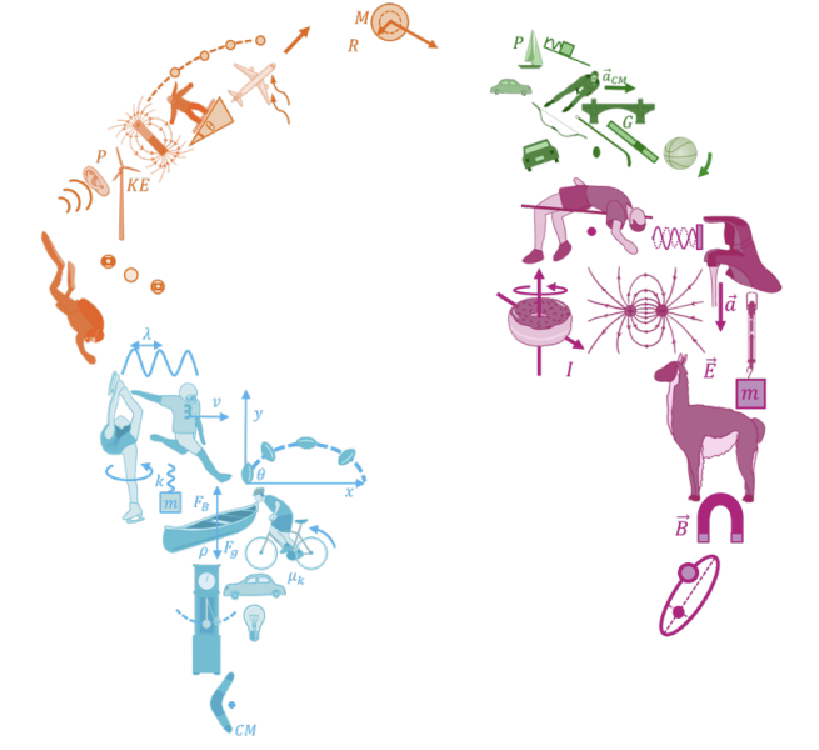
\includegraphics[width=4cm]{figures/BMDW/logo}
\end{textblock*}

\end{frame}

%%%%%%%%%%%%%TOC
\twocolframe{Outline}
  {\tableofcontents[sections={64,65}, subsectionstyle=show/show]\thispagestyle{empty}}
  {\tableofcontents[sections={66}, subsectionstyle=show/show]}
%%%%%%%%%%%%%%%%%%%%%%%%%







%%%%%%%%%%%%%%%%%%%%%%%%%%%%%%%%
\section{Faraday's Law}
\label{sec:faradayslaw}
\title{Faraday's Law}


%%%%%%%%%%%%%%%%%%%%%%%%%
\begin{frame}
\titlepage
\thispagestyle{empty}
\end{frame}

%%%%%%%%%%%%%%%%%%%%%%%




\subsection{Electromagnetism}
\label{subsec:electromagnetism}
\twocolframesf{Electromagnetism}
{
\begin{itemize}
\item So far, we have looked at static cases:
\begin{enumerate}
\item An electric field that does not change with time (e.g. created by a charge that is not moving)
\item A magnetic field that does not change with time (e.g. created by a current that is constant)
\end{enumerate}
\item<1> We have seen three of the four equations that explain all of electromagnetic phenomena
\item<2> Faraday’s law (the 4th equation) connects electric and magnetic fields
\item<2> Faraday’s law is the only one that explicitly references time
\end{itemize}
}
{
\only<1>{
\begin{align*}
\oint \vec E \cdot d\vec A &= \frac{Q^{enc}}{\epsilon_0}\\
\oint \vec B \cdot d\vec A &= 0\\
\oint \vec B \cdot d\vec l&= \mu_0 I^{enc}\\
\end{align*}
}
\only<2>{
\begin{align*}
\oint \vec E \cdot d\vec A &= \frac{Q{enc}}{\epsilon_0}\\
\oint \vec B \cdot d\vec A &= 0\\
\oint \vec B \cdot d\vec l&= \mu_0 I^{enc}\\
\oint \vec E \cdot d\vec l&= -\frac{d\Phi_B}{dt}\\
\end{align*}
Maxwell's equations (more or less...)
}

}

%%%%%%%%%%%%%%%%%%%%%%%%%%%%%%
\subsection{Formula}
\label{subsec:faradayformula}
\begin{bulletframe}{Faraday's Law}
\item The circulation of the electric field:
\begin{align*}
\oint \vec E \cdot d\vec l&= -\frac{d\Phi_B}{dt}
\end{align*}
\item This is zero, if $\frac{d\Phi_B}{dt}=0$, i.e. if $\Phi_B$  does not change with time (\textbf{statics}).
\pause
\item What is $\oint \vec E \cdot d\vec l$?
\begin{itemize}
\item Compare with the definition of electric potential difference:
\begin{align*}
\Delta V = (V_2-V_1) = -\int_{\vec r_1}^{\vec r_2}\vec E\cdot d\vec r
\end{align*}
\item $\oint \vec E \cdot d\vec l$ is the electric potential difference in going around a closed loop (ending where you started)
\item if $\Phi_B$  changes with time, then the electric field does net work when you go around a closed path $\rightarrow$ The electric force is no longer conservative!
\item Since $\Delta V$ in this case is the potential difference between two points that are the same, we (they) find it less awkward to call it emf (electromotive force).
\end{itemize}
\end{bulletframe}


%%%%%%%%%%%%%%%%%%%%%%%%%%%%%%
\subsection{EMF on a closed loop}
\label{subsec:emfonaclosedloop}
\twocolframesf{EMF on a closed loop}
{
\begin{itemize}
\item If a charge $q$ goes around the loop, it will gain energy given by:
\begin{align*}
W=q\Delta V
\end{align*}
\item If there is no way for the charge to loose energy (e.g. a resistor or air molecules), it will keep going around the circle faster and faster.
\item The loop does not need to be an actual physical wire, it can just be an arbitrarily drawn path.
\item If the loop is a wire, then the emf is like an ideal battery.
\end{itemize}
}
{
\centering
\begin{tikzpicture}[scale=1]
\tikzmath{
\R=2;
\d=0.1;
\L=0.5;
}

\draw[line width = 2.5pt] (0,0) circle(\R);
\draw[line width = 2.5pt] (\d,-\R-\L) -- (\d,-\R+\L);
\draw[line width = 2.5pt] (-\d,-\R-0.5*\L) -- (-\d,-\R+0.5*\L);

\draw[line width = 2.5pt,-latex] (30:1.2*\R) arc(30:60:1.2*\R) node[midway,right=5pt] {$\vec E$};

\node[below] at (0,-\R-\L) {$\Delta V$};
\end{tikzpicture}

}


%%%%%%%%%%%%%%%%%%%%%%%%%%%%%%
\subsection{Review: the galvonometer}
\label{subsec:reviewthegalvonometer}
\twocolframe{Review: the galvanometer}
{
\begin{itemize}
\item A coil carrying current has a magnetic dipole moment.
\item The coil wants to align its dipole moment with an external magnetic field.
\item A galvanometer is a very sensitive device for measuring current:
\begin{itemize}
\item When a current is present in the coil, the torque on the coil is proportional to current.
\item A balancing torque is provided by a restoring spring.
\end{itemize}
\end{itemize}
}
{
\capfig{0.9}{figures/Induction/galvanometer}{A galvanometer}
}



%%%%%%%%%%%%%%%%%%%%%%%%%%%%%%



%%%%%%%%%%%%%%%%%%%%%%%%%%%%%%



%%%%%%%%%%%%%%%%%%%%%%%%%%%%%%
\subsection{Induction}
\label{subsec:induction}
\twocolframe{Induction}
{
\begin{itemize}
\item Henry and Faraday both observed that currents can be induced with a magnet.
\item Faraday described it in more detail, so we refer to Faraday’s Law of Induction.
\item Currents were only induced when there was a change in the magnetic field.
\end{itemize}
}
{
\vspace{-2cm}
\capfig{1}{figures/Induction/faraday2}{Faraday's experiment showing induction between coils of wire: The liquid battery (right) provides a current which flows through the small coil (A), creating a magnetic field. When the coils are stationary, no current is induced. But when the small coil is moved in or out of the large coil (B), the magnetic flux through the large coil changes, inducing a current which is detected by the galvanometer (G). Wikipedia.}
}


%%%%%%%%%%%%%%%%%%%%%%%%%%%%%%
\begin{bulletframe}{More observations from Faraday}
\item The induced current is larger if the magnetic field is stronger.
\item The induced current is larger if the area of the loop is larger.
\item The induced current is larger if the magnet moves perpendicular to the loop.
\end{bulletframe}


%%%%%%%%%%%%%%%%%%%%%%%%%%%%%%
\subsection{Magnetic flux and Faraday's law of induction}
\label{subsec:magneticfluxandfaradayslawofinduction}
\twocolframesf{Magnetic Flux and Faraday's law of induction}
{
\begin{itemize}
\item \textbf{Magnetic flux} through area, $A$:
\begin{align*}
\Phi_B = \int \vec B \cdot d\vec A=\int BdA \cos\theta
\end{align*}
\end{itemize}
$\Delta V$ is the ``induced emf'' along the loop that bounds the area:
\begin{itemize}
\item Proportional to area of loop.
\item Proportional to magnetic field.
\item Proportional to rate of change of flux.
\item The opposite sign if $\vec B$ points in the opposite direction.
\end{itemize}
}
{
Faraday’s Law of induction:
\begin{align*}
\Delta V = -\frac{d\Phi_B}{dt}
\end{align*}
\centering

\begin{tikzpicture}[scale=0.5]
\tikzmath{
\L = 4;
\LA = 2.5;
\D=2.5;
}

\draw[color=qblue, line width =0.5] (\L,-\D,0) -- (0,0,0);

\fill[color=qred!80,opacity=0.7] (-\L/2,0,-\L/2) -- (-\L/2,0,\L/2) -- (\L/2,0,\L/2) -- (\L/2,0,-\L/2) -- cycle;
\draw[color=qred, line width = 1] (-\L/2,0,-\L/2) -- (-\L/2,0,\L/2) -- (\L/2,0,\L/2) -- (\L/2,0,-\L/2) -- cycle;

\draw[line width = 2, -latex, color=qred] (0,0,0) -- +(0,\LA,0) node[right]{$\vec A$};;
\draw[line width = 2, -latex, color=qblue] (0,0,0) -- ($(0,0,0)!0.75!(-\L,\D,0)$) node[above]{$\vec B$};;


\draw[color=qblue, line width =1] (0,0.3*\LA,0) arc (90:145:0.3*\LA) node[midway,above] {$\theta$};

\draw[color=qblue, line width =0.5] (0,0,0) -- (-\L,\D,0);


\end{tikzpicture}
\captionof*{figure}{\textit{Flux of magnetic field through an open surface. The potential difference in Faraday's Law is along the closed path that bounds the surface.}}
}



%%%%%%%%%%%%%%%%%%%%%%%%%%%%%%



%%%%%%%%%%%%%%%%%%%%%%%%%%%%%%
%%%%%%%%%%%%%%%%%%%%%%%%%%%%%%





\twocolframesf{Magnetic Flux and Faraday’s law of induction}
{
\begin{itemize}
\only<1>{\item We introduce \textbf{magnetic flux} through an area defined by a {\color{qred}loop} as:
\begin{align*}
\Phi_B = \int \vec B \cdot d\vec A=\int BdA \cos\theta
\end{align*}}
\item \textbf{Faraday’s Law} of induction:
\begin{align*}
\Delta V = -\frac{d\Phi_B}{dt}
\end{align*}
\end{itemize}
$\Delta V$ is the change in potential energy per unit charge from going around the {\color{qred}loop} once.
\only<2>{
\begin{itemize}
\item \textbf{Lenz’s Law} tells us which way the induced current goes around the loop (allowing us to ignore the minus sign):
\begin{itemize}
\item If the \textbf{flux is increasing} in the loop, then the induced current creates a magnetic field that is in the \textbf{opposite direction} of the original field.
\item If the \textbf{flux is decreasing} in the loop, then the induced current creates a magnetic field that is in the \textbf{same direction} as the original field.
\end{itemize}
\end{itemize}
}
}
{

\centering
\begin{tikzpicture}[scale=0.5]
\tikzmath{
\L = 4;
\LA = 2.5;
\D=2.5;
}

\draw[color=qblue, line width =0.5] (\L,-\D,0) -- (0,0,0);

\fill[color=qred!80,opacity=0.5] (-\L/2,0,-\L/2) -- (-\L/2,0,\L/2) -- (\L/2,0,\L/2) -- (\L/2,0,-\L/2) -- cycle;
\draw[color=qred, line width = 1] (-\L/2,0,-\L/2) -- (-\L/2,0,\L/2) -- (\L/2,0,\L/2) -- (\L/2,0,-\L/2) -- cycle;

\draw[line width = 2, -latex, color=qred] (0,0,0) -- +(0,\LA,0) node[right]{$\vec A$};;
\draw[line width = 2, -latex, color=qblue] (0,0,0) -- ($(0,0,0)!0.75!(-\L,\D,0)$) node[above]{$\vec B$};;


\draw[color=qblue, line width =1] (0,0.2*\LA,0) arc (90:145:0.2*\LA) node[midway,above] {$\theta$};

\draw[color=qblue, line width =0.5] (0,0,0) -- (-\L,\D,0);


\end{tikzpicture}
\captionof*{figure}{\textit{Flux of magnetic field through a surface enclosed by a loop.}}
}



%%%%%%%%%%%%%%%%%%%%%%%%%%%%%%
\subsection{Review: magnetic moment}
\label{subsec:reviewmagneticmoment}
\twocolframesf{Review: Magnetic moment}
{
\begin{itemize}
\item An induced current creates its own magnetic field.
\item The magnetic field in the loop is aligned with the magnetic moment of the induced current in the loop:
\begin{align*}
\vec\mu=I\vec A
\end{align*}
\item The loop is like a bar magnet with magnetic moment $\vec\mu$, thus it will experience a torque that will tend to align the magnetic moment with the magnetic field that is inducing the current:
\begin{align*}
\vec\tau = \vec\mu \times \vec B
\end{align*}
\end{itemize}

}
{
\vspace{-1.5cm}
\capfig{0.4}{figures/Induction/mu}{Magnetic moment for a loop of current.}
\vspace{-0.5cm}
\capfig{0.6}{figures/Induction/hand}{Right hand rule for axial vectors.}
}


%%%%%%%%%%%%%%%%%%%%%%%%%%%%%%
\subsection{The minus sign in Farada's law}
\label{subsec:theminussigninfaradayslaw}
\begin{bulletframe}{The minus sign in Faraday's Law}
\item The sign of the flux depends on the choice that we make for the direction of $d\vec A$.
\begin{align*}
\Delta V = -\frac{d\Phi_B}{dt}=\textcolor{qred}{-}\frac{d}{dt}\int \vec B \cdot d\vec A
\end{align*}
\item This will determine the sign of $\Delta V$.
\item Clearly, it's not arbitrary: If we look at current through a loop, it will flow in a given direction (from high V to low V, in the direction of $\vec E$).
\item The minus sign is there to conserve energy!
\item \textbf{It refers to the direction of the magnetic moment of the induced current relative to the (arbitrary) choice that was made for the direction of $d\vec A$.}
\end{bulletframe}


%%%%%%%%%%%%%%%%%%%%%%%%%%%%%%
\begin{bulletframe}{The minus sign in Faraday's Law}
\item The sign of the flux depends on the choice that we make for the direction of $d\vec A$:
\begin{align*}
\Delta V = -\frac{d\Phi_B}{dt} = -\frac{d}{dt}\int \vec B \cdot d\vec A
\end{align*}
\item This will determine the sign of $\Delta V$. \textbf{The easiest is to ignore the sign and use Lenz’s Law} to figure out which way the induced current goes.
\end{bulletframe}


%%%%%%%%%%%%%%%%%%%%%%%%%%%%%%
\twocolframest{The minus sign in Faraday's Law}
{
\begin{itemize}
\item However, the sign is meaningful, consider the case with the shrinking ring in a constant field:
\begin{itemize}
\item If we choose \textbf{$d\vec A$ into the page}, then $\Phi_B$ is positive and decreasing in magnitude, so \textbf{$\frac{d\Phi_B}{dt} $ is negative}.
\item \textbf{\color{qred}$\Delta V$ is thus positive}. 
\item With Lenz’s Law, we can argue that the current is clockwise. 
\item By choosing the direction of $d\vec A$, we define what we consider to be the positive direction of current (with our right hand). \textbf{The sign of $\Delta V$ tells us whether the magnetic moment from the induced current is in the same direction as our choice of $d\vec A$ }.
\item The magnetic moment of the induced current is in the \textbf{\color{qred}same direction} as $d\vec A$ in this case.
\end{itemize}
\end{itemize}
}
{
\begin{align*}
\Aboxed{\Delta V &= -\frac{d\Phi_B}{dt}= -\frac{d}{dt}\int \vec B \cdot d\vec A}
\end{align*}
\centering
\begin{tikzpicture}[scale=1]
\tikzmath{
\R=1.;
\d=0.1;
\L=0.5;
\Nt=3;
}

\foreach \i in {0,...,\Nt}{
  \foreach \j in {0,...,\Nt}{
    \tikzmath{
      \x=-1.5*\R+\i*3*\R/\Nt;
       \y=-1.5*\R+\j*3*\R/\Nt;
    }
    \node[color=qblue!80] at (\x,\y) {\Large $\times$};
  }
}
%arrows
\draw[->,color=qred,line width = 1pt] (-1.35*\R,0) -- (-\R,0);
\draw[->,color=qred,line width = 1pt] (-\R,0) -- (-0.65*\R,0);
\draw[->,color=qred,line width = 1pt] (1.35*\R,0) -- (\R,0);
\draw[->,color=qred,line width = 1pt] (\R,0) -- (0.65*\R,0);
\draw[->,color=qred,line width = 1pt] (0,1.35*\R) -- (0,\R);
\draw[->,color=qred,line width = 1pt] (0,\R) -- (0,0.65*\R);

%circles
\draw[line width = 2.5pt,color=qred] (0,0) circle(\R);
\draw[line width = 1pt, dashed, opacity=0.8,color=qred] (0,0) circle(1.35*\R);
\draw[line width = 1pt, dashed, opacity=0.8,color=qred] (0,0) circle(0.65*\R);

%battery
\draw[line width = 2.5pt,color=qred] (-\d,-\R-\L) -- (-\d,-\R+\L);
\draw[line width = 2.5pt,color=qred] (\d,-\R-0.5*\L) -- (\d,-\R+0.5*\L);

%current and voltage
\draw[line width = 2.5pt,latex-,color=qred] (30:1.2*\R) arc(30:60:1.2*\R) node[midway,right=5pt] {$I$};
\node[below,color=qred] at (0,-\R-\L) {$\Delta V$};

\node[color=qblue,above] at (1.5*\R,1.5*\R) {$\vec B$};

\node[] at (0,0) {$\times$};
\node[above] at (0,0) {$d\vec A$};

\end{tikzpicture}
\captionof*{figure}{\textit{A shrinking loop in a magnetic field into the page will have clocwkise induced current.}}
}


%%%%%%%%%%%%%%%%%%%%%%%%%%%%%%
\twocolframest{The minus sign in Faraday's Law}
{
\begin{itemize}
\item However, the sign is meaningful, consider the case with the shrinking ring in a constant field:
\begin{itemize}
\item If we choose \textbf{$d\vec A$ out of the page}, then $\Phi_B$ is negative and increasing in value (but decreasing in magnitude), so \textbf{$\frac{d\Phi_B}{dt} $ is positive}.
\item \textbf{\color{qred}$\Delta V$ is thus negative}. 
\item With Lenz’s Law, we can argue that the current is clockwise. 
\item By choosing the direction of $d\vec A$, we define what we consider to be the positive direction of current (with our right hand). \textbf{The sign of $\Delta V$ tells us whether the magnetic moment from the induced current is in the same direction as our choice of $d\vec A$ }.
\item The magnetic moment of the induced current is in the \textbf{\color{qred}opposite} direction as $d\vec A$ in this case.
\end{itemize}
\end{itemize}
}
{
\begin{align*}
\Aboxed{\Delta V &= -\frac{d\Phi_B}{dt}= -\frac{d}{dt}\int \vec B \cdot d\vec A}
\end{align*}
\centering
\begin{tikzpicture}[scale=1]
\tikzmath{
\R=1.;
\d=0.1;
\L=0.5;
\Nt=3;
}

\foreach \i in {0,...,\Nt}{
  \foreach \j in {0,...,\Nt}{
    \tikzmath{
      \x=-1.5*\R+\i*3*\R/\Nt;
       \y=-1.5*\R+\j*3*\R/\Nt;
    }
    \node[color=qblue!80] at (\x,\y) {\Large $\times$};
  }
}
%arrows
\draw[->,color=qred,line width = 1pt] (-1.35*\R,0) -- (-\R,0);
\draw[->,color=qred,line width = 1pt] (-\R,0) -- (-0.65*\R,0);
\draw[->,color=qred,line width = 1pt] (1.35*\R,0) -- (\R,0);
\draw[->,color=qred,line width = 1pt] (\R,0) -- (0.65*\R,0);
\draw[->,color=qred,line width = 1pt] (0,1.35*\R) -- (0,\R);
\draw[->,color=qred,line width = 1pt] (0,\R) -- (0,0.65*\R);

%circles
\draw[line width = 2.5pt,color=qred] (0,0) circle(\R);
\draw[line width = 1pt, dashed, opacity=0.8,color=qred] (0,0) circle(1.35*\R);
\draw[line width = 1pt, dashed, opacity=0.8,color=qred] (0,0) circle(0.65*\R);

%battery
\draw[line width = 2.5pt,color=qred] (-\d,-\R-\L) -- (-\d,-\R+\L);
\draw[line width = 2.5pt,color=qred] (\d,-\R-0.5*\L) -- (\d,-\R+0.5*\L);

%current and voltage
\draw[line width = 2.5pt,latex-,color=qred] (30:1.2*\R) arc(30:60:1.2*\R) node[midway,right=5pt] {$I$};
\node[below,color=qred] at (0,-\R-\L) {$\Delta V$};

\node[color=qblue,above] at (1.5*\R,1.5*\R) {$\vec B$};

\node[] at (0,0) {$\odot$};
\node[above] at (0,0) {$d\vec A$};

\end{tikzpicture}
\captionof*{figure}{\textit{A shrinking loop in a magnetic field into the page will have clocwkise induced current.}}
}

%%%%%%%%%%%%%%%%%%%%%%%%%%%%%%
\begin{bulletframe}{The minus sign in Faraday's Law}
\item Usually, can ignore and just use Lenz's Law (i.e. conservation of energy) to argue the direction of the induced current. 
\item If it's not clear, it's easiest to \textbf{pick $d\vec A$ so that $\vec B \cdot d\vec A>0$} (so that $d\vec A$ has at least a component parallel to $\vec B$).
\item Sometimes there's no choice (e.g. a rotating coil), you need to pay attention and be clear about your choice of $d\vec A$.

\end{bulletframe}

%%%%%%%%%%%%%%%%%%%%%%%%%%%%%%






%%%%%%%%%%%%%%%%%%%%%%%%%%%%%%%%
\section{Lenz's Law}
\label{sec:lenzslaw}
\title{Lenz's Law}


%%%%%%%%%%%%%%%%%%%%%%%%%
\begin{frame}
\titlepage
\thispagestyle{empty}
\end{frame}

%%%%%%%%%%%%%%%%%%%%%%%












%%%%%%%%%%%%%%%%%%%%%%%%%%%%%%%%%%%%%
\subsection{Conservation of energy to the rescue!}
\label{subsec:conservationofenergytotherescue}
\begin{bulletframe}{Conservation of energy to the rescue!}
\item The current induced in a coil will create its own magnetic field.
\begin{itemize}
\item Current in a coil creates a magnetic field, right?!
\end{itemize}
\item The total magnetic field is the ``original'' magnetic field plus the one created by the induced current.
\item[$\rightarrow$] If the magnetic field from the induced current changes the flux in a way to induce more current, then we are creating an infinite amount of current (and energy)! 
\item[$\rightarrow$] The induced current must create a magnetic field that opposes the change in flux of the original magnetic field.
\end{bulletframe}


%%%%%%%%%%%%%%%%%%%%%%%%%%%%%%%%%%%%




%%%%%%%%%%%%%%%%%%%%%%%%%%%%%%%%%%%%%7
\subsection{Theory}
\label{subsec:leztheory}
\begin{bulletframe}{Lenz's Law}
\item The induced current is in such a direction as to create a magnetic field that opposes the change in flux:
\begin{itemize}
\item If the \textbf{flux is increasing} in the loop, then the induced current creates a magnetic field that is in the \textbf{opposite direction} of the original field.
\item If the \textbf{flux is decreasing} in the loop, then the induced current creates a magnetic field that is in the \textbf{same direction} as the original field.
\end{itemize}

\end{bulletframe}

%%%%%%%%%%%%%%%%%%%%%%%%%%%%%%%%%%%%%

\twocolframe{Lenz's Law}
{
\begin{itemize}
\item The magnetic field flux above the magnet decreases if the magnet falls down.
\begin{itemize}
\item A current is induced to create a magnetic field to restore the flux
\item That magnetic field attracts the magnet!
\end{itemize}
\end{itemize}
}
{
\capfig{0.75}{figures/Induction/lenz}{\url{http://physicsbuzz.physicscentral.com/2014/09/build-your-own-time-warp-tube.html}}
}


%%%%%%%%%%%%%%%%%%%%%%%%%%%%%%


%%%%%%%%%%%%%%%%%%%%%%%%%%%%%%
\subsection{Current in a coil with N loops}
\label{subsec:currentinacoilwithnloops}
\twocolframesf{Current in a coil with N loops}
{
\begin{itemize}
\item Each loop can be considered separately (each has an induced emf from the flux changing through it).
\item Each loop is like a little battery, and the loops are all in series.
\item The (identical) emfs from each loop just add together:
\begin{align*}
\Delta V = -N \frac{d\Phi_B}{dt}
\end{align*}
where $\Phi_B$ is the flux through one loop.
\end{itemize}

}
{
\centering
\begin{tikzpicture}[scale=0.75]

\tikzmath{
\R = 2.5;%charge radius
\f = 0.25;
\L = 1.5;
\Nt = 5;
\d=0.1;
\LV=0.5;
\LL=5;
}

%\draw[-latex] (0,0) -- (0,1.25*\R) node[left] {$y$};
%\draw[-latex] (0,0) -- (1.25*\R,0) node[below] {$x$};

\foreach \i in {0,...,\Nt}{
 \tikzmath{
 \h = -\L/2+\i*\L/\Nt;
 \hb=-\R+\i*2*\R/\Nt;
 \xl=-\LL/2+\i*\LL/\Nt;
 }
 
 %batteries
 \draw[line width = 1.5pt] (\xl+\d,-1.5*\R-\LV) -- (\xl+\d,-1.5*\R+\LV) node[above]{\tiny $\Delta V_i$ };
 \draw[line width = 1pt] (\xl+\d,-1.5*\R) -- (\xl+5*\d,-1.5*\R);
 \draw[line width = 1pt] (\xl-5*\d,-1.5*\R) -- (\xl-\d,-1.5*\R);
 \draw[line width = 1.5pt] (\xl-\d,-1.5*\R-0.5*\LV) -- (\xl-\d,-1.5*\R+0.5*\LV);
 
 %loops
 \draw[line width=2] (\h,-\R) arc(270:90:{\R*\f} and {\R});
 \draw[line width=1.5, dotted] (\h,\R) arc(90:-90:{\R*\f} and {\R});

 %mag field arrows 
 \draw[-latex, line width =2, color = qblue] (1.1*\R,\hb) -- + (-0.5*\R,0);
}

\node[color=qblue] at (1.1*\R,0) {$\vec B(t)$};
\node at (0,-1.5*\R-2*\LV) {$\Delta V = N\Delta V_i$};


\end{tikzpicture}
}


%%%%%%%%%%%%%%%%%%%%%%%%%%%%%%
\subsection{Motional emf}
\twocolframesf{Motional emf}
{
\begin{itemize}
\item Refers specifically to the case when the magnetic field is constant and the change in flux comes from motion:
\begin{align*}
\Phi_B=\int \vec B\cdot d\vec A=\int BdA\cos\theta
\end{align*}
\end{itemize}
Two options:
\begin{enumerate}
\item The angle  is changing with time (a generator).
\item The area of the loop is changing with time (the sliding bar).
\end{enumerate}

}
{
\capfig{0.7}{figures/Induction/motor}{Flux is changed by rotation.}


\centering
\begin{circuitikz}[scale=0.75]

\tikzmath{
\L=5;
\h=2;
\Nt=8;
\Lv=1;
}

%bfield
\foreach \i in {1,...,7}{
 \tikzmath{
 \x = -\L/2+\i*\L/\Nt;
 }
 \node[color=qblue!80] at (\x,0.25*\h) {\Large $\odot$};
 \node[color=qblue!80] at (\x,-0.25*\h) {\Large $\odot$};
}


\draw [color=gray, line width=5pt] (-\L/2,\h/2) -- (\L/2,\h/2);
\draw [color=gray, line width=5pt] (-\L/2,-\h/2) -- (\L/2,-\h/2);


\draw [color=black, line width=3pt] (-0.*\L,-\h/2) -- (-0.*\L,\h/2);
\draw [color=black, line width=1.5pt,-latex] (0.*\L,0) -- +(-\Lv,0) node[left]{$\vec v$};

\draw (\L/2,\h/2) [R=$R$] to (\L/2,-\h/2);
\node[color=qblue] at (0.25*\L,0) {$\vec B$};
\draw[latex-latex] (-0.55*\L, -0.5*\h) -- (-0.55*\L, 0.5*\h) node[midway,left] {$l$};


\end{circuitikz}
\captionof*{figure}{\textit{Flux is changed by change in area.}}
}


%%%%%%%%%%%%%%%%%%%%%%%%%%%%%%


%%%%%%%%%%%%%%%%%%%%%%%%%%%%%%
\subsection{A bar moving on rails}
\twocolframesf{A bar moving on rails}
{\scriptsize
\begin{itemize}
\item<1-> The area increases with time:%
\begin{align*}%
A=l(w_0+vt)%
\end{align*}%
\item<2-> The flux is ($\vec A$ out of the page):%
\begin{align*}%
\Phi_B(t)=AB=Bl(w_0+vt)%
\end{align*}%
\item<3-> The induced emf:%
\begin{align*}%
\Delta V=-\frac{d\Phi_B}{dt}=-Blv%
\end{align*}%
\item<4-> The induced current:%
\begin{align*}%
I=\frac{\Delta V}{R}=-\frac{Blv}{R}%
\end{align*}%
\only<4->{
(negative, $\vec \mu$ into the page since $\vec A$ out of the page, clockwise current)
}
\end{itemize}
}
{

\centering
\begin{circuitikz}[scale=1]

\tikzmath{
\L=4.5;
\h=2;
\Nt=8;
\Lv=1;
\xb=0;
}

%bfield
\foreach \i in {1,...,7}{
 \tikzmath{
 \x = -\L/2+\i*\L/\Nt;
 }
 \node[color=qblue!80] at (\x,0.25*\h) {\Large $\odot$};
 \node[color=qblue!80] at (\x,-0.25*\h) {\Large $\odot$};
}


\draw [color=gray, line width=5pt] (-\L/2,\h/2) -- (\L/2,\h/2);
\draw [color=gray, line width=5pt] (-\L/2,-\h/2) -- (\L/2,-\h/2);


\draw [color=black, line width=3pt] (\xb,-\h/2) -- (\xb,\h/2);
\draw [color=black, line width=1.5pt,-latex] (\xb,0) -- +(-\Lv,0) node[left]{$\vec v$};

\draw (\L/2,\h/2) [R=$R$] to (\L/2,-\h/2);
\node[color=qblue] at (0.25*\L,0) {$\vec B$};
\draw[latex-latex] (-0.55*\L, -0.5*\h) -- (-0.55*\L, 0.5*\h) node[midway,left] {$l$};
\draw[latex-latex] (0.5*\L, 0.6*\h) -- (\xb, 0.6*\h) node[midway,above] {$w(t)=w_0+vt$};


\only<5>{

\node[color=qred] at (\xb+0.2,\h/2) {$+$};
\node[color=qred] at (\xb-0.2,\h/2) {$+$};
\node[color=qred] at (\xb+0.2,0.4*\h) {$+$};
\node[color=qred] at (\xb-0.2,0.4*\h) {$+$};
\node[color=qred] at (\xb+0.2,0.3*\h) {$+$};
\node[color=qred] at (\xb-0.2,0.3*\h) {$+$};

\node[color=qred] at (\xb+0.2,-\h/2) {$-$};
\node[color=qred] at (\xb-0.2,-\h/2) {$-$};
\node[color=qred] at (\xb+0.2,-0.4*\h) {$-$};
\node[color=qred] at (\xb-0.2,-0.4*\h) {$-$};
\node[color=qred] at (\xb+0.2,-0.3*\h) {$-$};
\node[color=qred] at (\xb-0.2,-0.3*\h) {$-$};
}

\end{circuitikz}
\captionof*{figure}{\textit{A bar moving on rails.}}

\only<5->{
\vspace{-1cm}
\begin{exampleblock}{Remember the Hall Effect?}
\tiny
\begin{itemize}
\item Free charges feel a magnetic force:
\begin{align*}
F_B=qvB
\end{align*}
\item Equilibrium between the electric and magnetic forces:
\begin{align*}
qvB=qE=q\frac{\Delta V}{l} \quad \rightarrow \quad \Delta V = Blv
\end{align*}
\end{itemize}
The emf exists event if there is no closed loop or rails!
\end{exampleblock}
}


}


%%%%%%%%%%%%%%%%%%%%%%%%%%%%%%



%%%%%%%%%%%%%%%%%%%%%%%%%%%%%%
\twocolframesf{A bar moving on rails}
{\scriptsize
\begin{itemize}
\item The induced current:
\begin{align*}%
I=\frac{\Delta V}{R}=-\frac{Blv}{R}%
\end{align*}%
\item The magnitude of the magnetic force on the bar is:
\begin{align*}%
F=IlB=\frac{B^2l^2v}{R}
\end{align*}%
\item The power to move the bar is (force exerted at constant speed):
\begin{align*}%
P=Fv=\frac{B^2l^2v^2}{R}
\end{align*}%
\item The power dissipated in the resistor is:
\begin{align*}%
P=I^2R=\frac{B^2l^2v^2}{R}
\end{align*}%
\end{itemize}
}
{

\centering
\begin{circuitikz}[scale=1]

\tikzmath{
\L=4.5;
\h=2;
\Nt=8;
\Lv=1;
\xb=0;
}

%bfield
\foreach \i in {1,...,7}{
 \tikzmath{
 \x = -\L/2+\i*\L/\Nt;
 }
 \node[color=qblue!80] at (\x,0.25*\h) {\Large $\odot$};
 \node[color=qblue!80] at (\x,-0.25*\h) {\Large $\odot$};
}


\draw [color=gray, line width=5pt] (-\L/2,\h/2) -- (\L/2,\h/2);
\draw [color=gray, line width=5pt] (-\L/2,-\h/2) -- (\L/2,-\h/2);


\draw [color=black, line width=3pt] (\xb,-\h/2) -- (\xb,\h/2);
\draw [color=black, line width=1.5pt,-latex] (\xb,0) -- +(-\Lv,0) node[left]{$\vec v$};
\draw [color=qred, line width=1.5pt,-latex] (\xb,0) -- +(\Lv,0) node[right]{$\vec F$};
\draw [color=black, line width=3pt,-latex] (0,0) -- +(0,0.75) node[right]{$I$};

\draw (\L/2,\h/2) [R=$R$] to (\L/2,-\h/2);
%\node[color=qblue] at (0.25*\L,0) {$\vec B$};
\draw[latex-latex] (-0.55*\L, -0.5*\h) -- (-0.55*\L, 0.5*\h) node[midway,left] {$l$};
\draw[latex-latex] (0.5*\L, 0.6*\h) -- (\xb, 0.6*\h) node[midway,above] {$w(t)=w_0+vt$};


\end{circuitikz}
\captionof*{figure}{\textit{There is a force on the bar from the induced current}}

%\vspace{-1cm}
\begin{exampleblock}{Conservation of energy}
\scriptsize
The force has to oppose the motion, or you would get free current!\\
The rate at which work is done to pull the bar is the same as the rate at which energy is dissipated in the resistor.
\end{exampleblock}


}


%%%%%%%%%%%%%%%%%%%%%%%%%%%%%%%%%%%%%








%%%%%%%%%%%%%%%%%%%%%%%%%%%%%%%%
\section{Real World Examples}
\label{sec:realworldsexamples}
\title{Real World Examples}


%%%%%%%%%%%%%%%%%%%%%%%%%
\begin{frame}
\titlepage
\thispagestyle{empty}
\end{frame}

%%%%%%%%%%%%%%%%%%%%%%%







%%%%%%%%%%%%%%%%%%%%%%%%%%

\subsection{The generator}
\label{subsec:thegenerator}
\twocolframesf{The Generator}
{
\begin{itemize}
\item Convert mechanical work into electrical energy.
\item You have to do work (exert a torque) to keep a coil spinning in a magnetic field.
\item The work is usually done by a turbine.
\item The turbine is powered by:
\begin{itemize}
\item High pressure water from a change in height (hydro power).
\item High pressure steam created from a heat source (nuclear fission, fossil fuel burning).
\end{itemize}
\item Wind and tides can also be used to rotate a coil in a magnetic field.
\end{itemize}
}
{
\vspace{-1cm}
\capfig{0.9}{figures/Induction/turbine1}{https://www.researchgate.net/figure/Typical-steam-turbine\_fig2\_337794013}
\vspace{-1cm}
\capfig{0.9}{figures/Induction/turbine2}{https://3dprintingindustry.com/news/general-electric-oil-gas-use-robotics-3d-printing-80689}
}



%%%%%%%%%%%%%%%%%%%%%%%%%%%%%%




%%%%%%%%%%%%%%%%%%%%%%%%%%%%%%
\subsubsection{Modelling a generator}
\label{subsubsec:modellingagenerator}
\twocolframesf{Modelling a generator}
{
\begin{itemize}
\item<1-> We rotate a coil about the $y$ axis with an angular velocity $\vec\omega=\omega\hat y$ in a constant magnetic field, $\vec B=B\hat x$. 
\item<2-> We choose $\vec A$ to be in the $\hat x$ direction at $t=0$:
\begin{align*}
\vec A = A(\cos(\omega t)\hat x - \sin(\omega t)\hat z)
\end{align*}
\item<3-> The induced EMF is (for N loops in the coil):
\begin{align*}
\Delta V = -N \frac{d\Phi_B}{dt}= -N \frac{d}{dt}\vec A\cdot \vec B=NAB\omega\sin(\omega t)
\end{align*}
\end{itemize}
\only<3->{
\scriptsize
This leads to sinusoidal (AC) voltage. Since $\Delta V$ changes sign as a function of time, the induced current keeps changing direction (relative direction of $\vec A$ and $\vec \mu$).
}

}
{
\vspace{-1cm}
\centering
\begin{tikzpicture}[scale=0.9]
\tikzmath{
\R=1;
\f=0.25;
\Nb=5;
\LB=0.75;
}

%axes:
 \draw[-latex] (0,0) -- (1.75*\R,0) node[below]{$x$}; 
 \draw[-latex] (0,0) -- (0,1.75*\R) node[left]{$y$}; 
 \draw[-latex] (0,0) -- (-\f*1.75*\R,-\f*1.75*\R) node[left]{$z$}; 
%back of ring
 \draw[line width=1.5, dotted, color=qred] (0,\R) arc(90:-90:{\R*\f} and {\R});
%B-field
 \foreach \i in {0,...,\Nb}{
 \tikzmath{
   \h=-1.25*\R+\i*2.5*\R/\Nb;
  }
  \draw[color=qblue!80,-latex,line width = 1.5] (-\LB,\h) -- +(\LB,0);
 }
 %front of ring
 \draw[line width=2, color=qred] (0,-\R) arc(270:90:{\R*\f} and {\R});
 
 \node[color=qblue!80] at (-1.25*\R,0) {$\vec B$};
 \draw[line width=2, color=black, -latex] (0,2*\R) -- +(0,\LB) node[right] {$\vec \omega$};
\end{tikzpicture}
%\vspace{0.8cm}
\captionof*{figure}{\textit{Side view at time $t=0$.}}
%
%
\vspace{-0.2cm}
%%%%%%%%%%%%%%%%%%5top view
\begin{tikzpicture}[scale=0.9]
\tikzmath{
\R=0.9;
\Rsq=\R/sqrt(2);
\f=0.25;
\Nb=5;
\LB=0.75;
\Ra=0.5;
}

%axes:
 \draw[-latex] (0,0) -- (1.75*\R,0) node[below]{$x$}; 
 \draw[-latex] (0,0) -- (0,-1.75*\R) node[left]{$z$}; 

%B-field
 \foreach \i in {0,...,\Nb}{
 \tikzmath{
   \h=-1.25*\R+\i*2.5*\R/\Nb;
  }
  \draw[color=qblue!80,-latex,line width = 1.5] (-\LB,\h) -- +(\LB,0);
 }

 \draw[line width=2, color=qred] (-\Rsq,\Rsq) -- (\Rsq,-\Rsq);
 \draw[line width=1.5, color=qred,-latex] (0,0) -- (\Rsq,\Rsq) node[above]{$\vec A$};
 \draw[line width=1.,-latex] (\Ra,0) arc (0:45:\Ra) node[midway,right] {$\omega t$};
 \node[color=qblue!80] at (-1.25*\R,0) {$\vec B$};
\end{tikzpicture}
\captionof*{figure}{\textit{Top view at time $t$.}}

}



%%%%%%%%%%%%%%%%%%%%%%%%%%%%%%
\subsubsection{Magnetic moment and torque}
\label{subsubsec:magneticmomentandtorque}
\twocolframesf{Generator: magnetic moment and torque}
{\scriptsize
\begin{itemize}
\item<1-> The induced EMF is (for N loops in the coil):
\begin{align*}
\Delta V = -N \frac{d\Phi_B}{dt}= -N \frac{d}{dt}\vec A\cdot \vec B=NAB\omega\sin(\omega t)
\end{align*}
\item<2-> If the coil has resistance R:
\begin{align*}
\vec\mu&=I\vec A = \frac{\Delta V}{R}\vec A\\
&=\frac{NAB\omega}{R}\sin(\omega t)A(\cos(\omega t)\hat x - \sin(\omega t)\hat z)
\end{align*}
\item<3-> The torque on the loop from the magnetic field is thus:
\begin{align*}
\vec\tau=\vec\mu\times\vec B=\frac{NA^2B^2\omega}{R}\sin^2(\omega t)(-\hat y)
\end{align*}
\end{itemize}
\only<3->{
\vspace{-0.5cm}
\scriptsize
We must thus exert a torque in the positive y direction (same direction as angular velocity) opposite of the torque from the magnetic field to keep the coil rotating at constant speed.
}

}
{
\vspace{-1cm}
\centering
\begin{tikzpicture}[scale=0.9]
\tikzmath{
\R=1;
\f=0.25;
\Nb=5;
\LB=0.75;
}

%axes:
 \draw[-latex] (0,0) -- (1.75*\R,0) node[below]{$x$}; 
 \draw[-latex] (0,0) -- (0,1.75*\R) node[left]{$y$}; 
 \draw[-latex] (0,0) -- (-\f*1.75*\R,-\f*1.75*\R) node[left]{$z$}; 
%back of ring
 \draw[line width=1.5, dotted, color=qred] (0,\R) arc(90:-90:{\R*\f} and {\R});
%B-field
 \foreach \i in {0,...,\Nb}{
 \tikzmath{
   \h=-1.25*\R+\i*2.5*\R/\Nb;
  }
  \draw[color=qblue!80,-latex,line width = 1.5] (-\LB,\h) -- +(\LB,0);
 }
 %front of ring
 \draw[line width=2, color=qred] (0,-\R) arc(270:90:{\R*\f} and {\R});
 
 \node[color=qblue!80] at (-1.25*\R,0) {$\vec B$};
 \draw[line width=2, color=black, -latex] (0,2*\R) -- +(0,\LB) node[right] {$\vec \omega$};
\end{tikzpicture}
%\vspace{0.8cm}
\captionof*{figure}{\textit{Side view at time $t=0$.}}
%
%
\vspace{-0.2cm}
%%%%%%%%%%%%%%%%%%5top view
\begin{tikzpicture}[scale=0.9]
\tikzmath{
\R=0.9;
\Rsq=\R/sqrt(2);
\f=0.25;
\Nb=5;
\LB=0.75;
\Ra=0.5;
}

%axes:
 \draw[-latex] (0,0) -- (1.75*\R,0) node[below]{$x$}; 
 \draw[-latex] (0,0) -- (0,-1.75*\R) node[left]{$z$}; 

%B-field
 \foreach \i in {0,...,\Nb}{
 \tikzmath{
   \h=-1.25*\R+\i*2.5*\R/\Nb;
  }
  \draw[color=qblue!80,-latex,line width = 1.5] (-\LB,\h) -- +(\LB,0);
 }

 \draw[line width=2, color=qred] (-\Rsq,\Rsq) -- (\Rsq,-\Rsq);
 \draw[line width=1.5, color=qred,-latex] (0,0) -- (\Rsq,\Rsq) node[above]{$\vec A$};
 \draw[line width=1.,-latex] (\Ra,0) arc (0:45:\Ra) node[midway,right] {$\omega t$};
 \node[color=qblue!80] at (-1.25*\R,0) {$\vec B$};
\end{tikzpicture}
\captionof*{figure}{\textit{Top view at time $t$.}}

}


%%%%%%%%%%%%%%%%%%%%%%%%%%%%%%
\subsubsection{Generator or motor?}
\label{subsubsec:generatorormotor}
\twocolframesf{Generator or Motor?}
{
\begin{itemize}
\item If we do mechanical work, we can rotate a coil in a magnetic field and induce a current:
\begin{itemize}
\item Mechanical energy $\rightarrow$ Electrical energy
\end{itemize}
\item If we instead apply a voltage to drive a current in the coil, the coil starts to rotate (an electric motor)
\begin{itemize}
\item Electrical energy $\rightarrow$ Mechanical energy
\end{itemize}
\item So what about the bar on rails? If we pull on the bar, we can induce a current. What if we instead apply a voltage? What happens? What’s that called?\only<2>{ A railgun...}
\end{itemize}
}
{
\only<1>{
\begin{columns}
\column{0.5\textwidth}
\capfig{0.9}{figures/Induction/turbine1}{A turbine.}
\column{0.5\textwidth}
\capfig{0.9}{figures/Induction/motor2-0}{A motor.}
%\animategraphics[loop,width=0.9\textwidth]{10}{figures/motor2-}{0}{2}
\end{columns}
\capfig{0.9}{figures/Induction/bar}{A bar on rails.}
}
}


%%%%%%%%%%%%%%%%%%%%%%%%%%%%%%
\subsection{The induced electric field}
\label{subsec:theinducedelectricfield}
\begin{bulletframe}{The induced electric field}
\item Faraday’s original formulation was in terms of induced voltage:
\begin{align*}
\Delta V = -\frac{d\Phi_B}{dt}
\end{align*}
\item But we can think of this in terms of induced electric field:
\begin{align*}
\oint \vec E\cdot d\vec l = -\frac{d\Phi_B}{dt}
\end{align*}
since, after all, voltage is just (negative) work done per unit charge by an electric field.
\end{bulletframe}




%%%%%%%%%%%%%%%%%%%%%%%%%%%%%%
\begin{bulletframe}{The induced electric field}
\item If we want to be able to calculate an electric field from:
\begin{align*}
\oint \vec E\cdot d\vec l
\end{align*}
Then, it’s easier if the integral is easy…
\item[$\rightarrow$] High degree of symmetry:
\begin{itemize}
\item $\vec E$ constant magnitude around the loop.
\item $\vec E$ and $d\vec l$ make a constant angle between them.
\end{itemize}
\item Same constraints as for Ampère’s Law!
\end{bulletframe}


%%%%%%%%%%%%%%%%%%%%%%%%%%%%%%
\twocolframesf{The induced electric field}
{
\begin{itemize}
\item Consider the uniform magnetic field inside of a solenoid. Assume that current is changing, so that magnetic field changes magnitude.
\item<2-> By symmetry, we expect the electric field to make concentric circles that are coaxial with the solenoid
\item<3> Choose a loop over which to calculate the circulation and flux:.
\begin{align*}
\oint \vec E\cdot d\vec l &=E(2\pi r)= -\frac{d\Phi_B}{dt}\\
\therefore E&=\frac{-1}{2\pi r}\frac{d\Phi_B}{dt}
\end{align*}
\end{itemize}
}
{
\centering
\begin{tikzpicture}[scale=1.0]
\tikzmath{
\R=3;
\r=0.6*\R;
\Nb=11;
\LB=1;
}


 \draw[line width=1.5] (0,0) circle(\R);
%B-field
\begin{scope}
\clip (0,0) circle(\R);
 \foreach \i in {0,...,\Nb}{
 \foreach \j in {0,...,\Nb}{
 \tikzmath{
   \x=-\R+\i*2*\R/\Nb;
   \y=-\R+\j*2*\R/\Nb;
  }
  \node[color=qblue!80] at (\x,\y) {\Large $\odot$};
 }}
 \end{scope}

\node[color=qblue!80, right=6pt] at (135:\R) {$\vec B$};
\draw[color=qred,line width = 2, -latex] (80:\R) arc (80:110:\R) node[midway,above] {$I$};

\only<2->{
\draw[color=qred, line width=1,-latex] (\r,0) -- +(0,\LB) node[right]{$\vec E$};
\draw[color=qred, line width=1,-latex] (-\r,0) -- +(0,-\LB) node[left]{$\vec E$};
\draw[color=qred, line width=1,-latex] (0,\r) -- +(-\LB,0) node[above]{$\vec E$};
\draw[color=qred, line width=1,-latex] (0,-\r) -- +(\LB,0) node[below]{$\vec E$};
}

\only<3>{
\draw[color=qred, line width=1] (0,0) circle(\r);
\draw[color=qred, line width=1] (0,0) -- (45:\r) node[midway,below] {$r$};

}

\end{tikzpicture}
\captionof*{figure}{\textit{A time varying magnetic field induces an electric field.}}
}


%%%%%%%%%%%%%%%%%%%%%%%%%%%%%%




%%%%%%%%%%%%%%%%%%%%%%%%%%%%%%
\subsection{Magnetic braking}
\twocolframesf{Magnetic braking}
{
\begin{itemize}
\item In the part entering the magnetic field, magnetic flux is increasing so a current is induced to create a magnetic field in the opposite direction.
\item In the part exiting the magnetic field,, the magnetic flux is decreasing, so a current is induced to create a magnetic field in the same direction.
\item At the middle, the currents from all loops go in the same direction, the force on those currents slow the disk down!
\end{itemize}
}
{
\vspace{-1cm}
\capfig{0.75}{figures/Induction/mbrake}{Magnetic brake.}
\vspace{-1cm}
\capfig{0.75}{figures/Induction/magneticbrake}{Magnetic brake (note that the field is in the opposite direction compared to above!). }
}


%%%%%%%%%%%%%%%%%%%%%%%%%%%%%%



%%%%%%%%%%%%%%%%%%%%%%%%%%%%%%
\subsection{Transformers}
\label{subsec:transformers}
\twocolframesf{Transformers}
{
\begin{itemize}
\item Used to change voltage.
\item Input coil generates changing magnetic flux (AC current).
\item Changing magnetic flux induces current (voltage) on output coil:
\begin{align*}
\Delta V_p &= -N_p\frac{d\Phi_B}{dt}\\
\Delta V_s &= -N_s\frac{d\Phi_B}{dt}\\
\therefore \frac{\Delta V_s}{\Delta V_p}=\frac{N_s}{N_p} \;\;&\rightarrow\;\; \Delta V_s=\frac{N_s}{N_p}\Delta V_p
\end{align*}
\end{itemize}
}
{
\vspace{-1cm}
\capfig{0.7}{figures/Induction/transformer}{A transformer.}
\vspace{-1cm}
\capfig{0.7}{figures/Induction/transpic}{\url{https://en.wikipedia.org/wiki/Transformer}}
}


%%%%%%%%%%%%%%%%%%%%%%%%%%%%%%



%%%%%%%%%%%%%%%%%%%%%%%%%%%%%%
\subsection{Power lines}
\label{subsec:powerlines}
\twocolframest{Power lines}
{\scriptsize
\begin{itemize}
\item Suppose that we wish to transmit 120kW through power lines with a resistance of $R=\SI{0.4}{\Omega}$. How much power do we loose in the lines?
\item We don't know the resistance of the load (the town), but we know how much power is going through the lines (the power from the plant is used in the lines and in the town), we can thus find the current:
\begin{align*}
P_{plant}=I\Delta V\;\;\rightarrow\;\; I=\frac{P_{plant}}{\Delta V}
\end{align*}
\item The power dissipated in the lines is:
\begin{align*}
P_{line}=I^2R_{line}=\frac{P^2_{plant}}{\Delta V^2}R_{line}
\end{align*}
\item If we transmit the power at \SI{240}{V}, $P_{line}=\SI{100}{kW}$ (more than 80\% loss)
\item If we transmit the power at \SI{24000}{V}, $P_{line}=\SI{10}{W}$  (much less than 1\% loss)
\end{itemize}
}
{
\capfig{0.7}{figures/Induction/powerplant}{A power plant connected to a city.}
}



%%%%%%%%%%%%%%%%%%%%%%%%%%%%%%
\subsection{Electric motor and EMF}
\label{subsec:electricmotorandemf}
\begin{bulletframe}{Electric motor and EMF}
\item Recall the electric motor:
\begin{itemize}
\item By running a current through a coil in a magnetic field, we could make the coil rotate
\item But now, we have a coil rotating in a magnetic field, so there must be an induced current in it, in addition to the current that we put in!
\end{itemize}
\end{bulletframe}




%%%%%%%%%%%%%%%%%%%%%%%%%%%%%%
\subsection{Effects of back EMF}
\label{subsec:effectsofbackemf}
\twocolframest{Back EMF}
{\scriptsize
\begin{itemize}
\item In order to conserve energy, the induced current is in the opposite direction of the current driving the motor.
\item The motor acts like a battery trying to oppose current coming in $\rightarrow$ ``back emf''.
\item When you first turn the motor on, no back emf, large current through the motor.
\item As the motor spins up, the back emf grows and the current decreases.
\item If there is no load on the motor, the back emf grows until it is just less than the driving emf (when it reaches the driving emf, the current is zero, the motor slows, the back emf goes down, the current goes back up $\rightarrow$ an equilibrium is reached).
\item In practice there is always a load from friction.
\item With no back emf, the motor would spin infinitely fast.
\end{itemize}
}
{
\capfig{0.7}{figures/Induction/backemf}{The back emf from a spinning motor acts like a battery that opposes current in a circuit. As the motor comes to speed, the back emf grows until an equlibrium is reached.}
}

%%%%%%%%%%%%%%%%%%%%%%%%%%%%%%
\begin{bulletframe}{Effects of back EMF}
\item If there is a load on the motor, it cannot spin as fast, back emf goes down, current goes up:
\begin{itemize}
\item If the current is higher, the motor can do more mechanical work ($I^2R$).
\item If the load is too high, the current could be too high in the motor and overheat it and melt it (try blocking the air intake of your hair dryer).
\end{itemize}
\item When the motor first turns on, it draws the most current:
\begin{itemize}
\item When the motor in your fridge turns on, the lights in your house momentarily dim.
\item This is because the large current draw results in an appreciable voltage drop across the resistance of the electrical wires in your house.
\item Everything in the circuit gets less voltage until the motor spins up and its current goes back down.
\end{itemize}
\end{bulletframe}


%%%%%%%%%%%%%%%%%%%%%%%%%%%%%%
\begin{frame}{Effects of back EMF}
\begin{columns}[T]
%%
\scriptsize
\column{0.33\textwidth}
\centering
\begin{circuitikz}
\tikzmath{
\L=1.5;
\h=2.5;
}
\node[draw=black] (M) at (\L/2,\h) {Motor};
\draw (0,0) [short] to (0,\h/2) [nos] to (0,\h) [short] to (M.west); 
\draw (M.east) [short] to (\L,\h) [short] to (\L,0) to [battery1] (0,0); 
\draw (0,\h/2) [voltmeter,o-o] to (\L,\h/2);
\end{circuitikz}
\\
\textbf{Switch open (motor off)}
\begin{itemize}
\item No current through motor.
\item {\color{qred} Voltmeter (high resistance) measures battery voltage.}
\item Your lights see the same voltage as the voltmeter, they are brightest.
\end{itemize}
%%
\column{0.33\textwidth}
\centering
\begin{circuitikz}
\tikzmath{
\L=1.5;
\h=2.5;
}
\node[draw=black] (M) at (\L/2,\h) {Motor};
\draw (0,0) [short] to (0,\h) [short] to (M.west); 
\draw (M.east) [short] to (\L,\h) [short] to (\L,0) to [battery1] (0,0); 
\draw (0,\h/2) [voltmeter,o-o] to (\L,\h/2);
\end{circuitikz}
\\
\textbf{Switch closed (motor accelerating)}
\begin{itemize}
\item High current through motor (low resistance).
\item {\color{qred} Voltmeter measures low voltage, since most current bypasses.}
\item Your lights see the same voltage as the voltmeter, they are dim.
\end{itemize}
%%
\column{0.33\textwidth}
\centering
\begin{circuitikz}
\tikzmath{
\L=1.5;
\h=2.5;
}
\node[draw=black] (M) at (0.35*\L,\h) {Motor};
\draw (\L,0) [battery1] to (0,0) [short] to (0,\h) [short] to (M.west); 
\draw (M.east) [battery1,invert] to (\L,\h) [short] to (\L,0); 
\draw (0,\h/2) [voltmeter,o-o] to (\L,\h/2);
\end{circuitikz}
\\
\textbf{Switch closed (motor spinning)}
\begin{itemize}
\item Back emf from the motor reduces current in the motor.
\item {\color{qred} Voltmeter goes back up to battery voltage minus back emf voltage.}
\item Your lights almost as bright as before.
\end{itemize}
\end{columns}
\end{frame}


%%%%%%%%%%%%%%%%%%%%%%%%%%%
































%%%%%%%%%%%%%%%%%%%%%%%%%
%%%%%% START OF PRESENTATION %%%%%%
%%%%%%%%%%%%%%%%%%%%%%%%%
\title{Relativity}
\subject{History of Relativity, Einstein and Spacetime Phenomena}
\subtitle{Building Models to Describe our World}


%%%%%%%%%%%%%%%%%%%%%%%%%%%%%%
%%%%%%%%%%%%%%%%%%%%%



%%%%%%%%%%%%%%%%%%%%%%%%%
%%%%%% Title slide %%%%%%
%%%%%%%%%%%%%%%%%%%%%%%%%
\chaptertitle{Relativity}
\begin{frame}
\label{chap:relativity}
\titlepage
\thispagestyle{empty}

\begin{textblock*}{5cm}(11cm,4cm)
    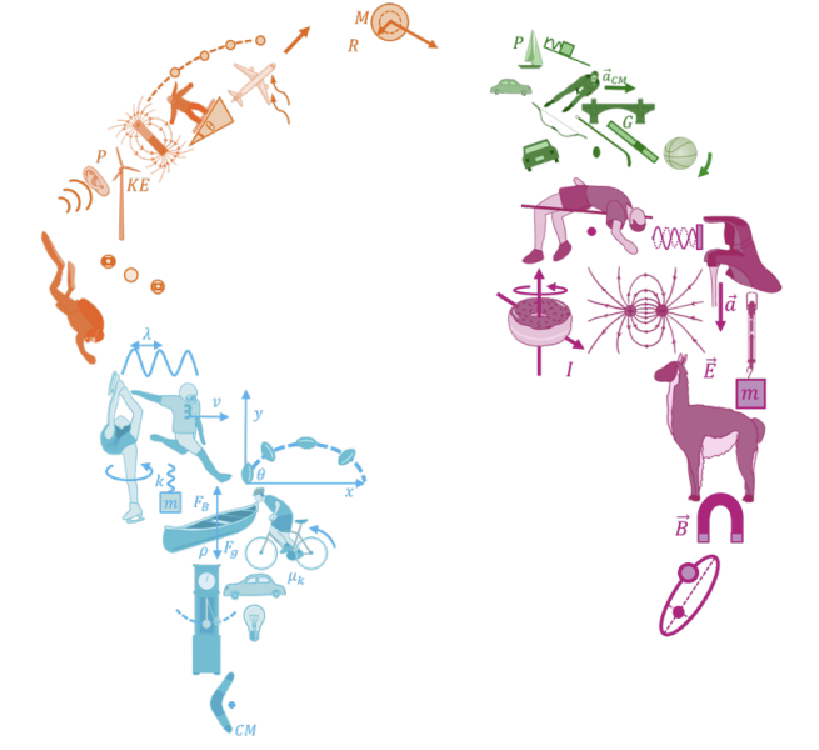
\includegraphics[width=4cm]{figures/BMDW/logo}
\end{textblock*}

\end{frame}

%%%%%%%%%%%%%TOC
\twocolframe{Outline}
  {\tableofcontents[sections={67}, subsectionstyle=show/show]\thispagestyle{empty}}
  {\tableofcontents[sections={68}, subsectionstyle=show/show]}
%%%%%%%%%%%%%%%%%%%%%%%%%



\twocolframe{Outline}
  {\tableofcontents[sections={69}, subsectionstyle=show/show]\thispagestyle{empty}}
  {}







%%%%%%%%%%%%%%%%%%%%%%%%%%%%%%%%
\section{History of Relativity}
\label{sec:historyofrelativity}
\title{History of Relativity}


%%%%%%%%%%%%%%%%%%%%%%%%%
\begin{frame}
\titlepage
\thispagestyle{empty}
\end{frame}

%%%%%%%%%%%%%%%%%%%%%%%%




\subsection{Maxwell's Equations}
\label{subsec:maxwellsequations}
\begin{bulletframe}{Maxwell's Equations}
\item So far we have seen several apparently disconnected topics in e/m:
\begin{itemize}
\item Coulomb’s law or Gauss’ law (we showed that these are equivalent):
\begin{align*}
\oint \vec E \cdot d\vec A = \frac{Q^{enc}}{\epsilon_0}
\end{align*}
\only<1>{\item Ampere’s law:
\begin{align*}
\oint \vec B \cdot d\vec l = \mu_0 I^{enc}
\end{align*}}
\only<2->{\item Ampere’s law (a little more generally):
\begin{align*}
\oint \vec B \cdot d\vec l = \mu_0 I^{enc} = \mu_0\int \vec j\cdot d\vec A+\mu_0\epsilon_0\frac{d}{dt}\int \vec E\cdot d\vec A
\end{align*}}
\item Faraday’s law:
\begin{align*}
\oint \vec E \cdot d\vec l = -\frac{d}{dt}\int \vec B\cdot d\vec A
\end{align*}
\item No magnetic monopoles (like Gauss’ law, but no such thing as magnetic charge):
\begin{align*}
\oint \vec B \cdot d\vec A = 0
\end{align*}
\end{itemize}
\item<2->[$\rightarrow$]\color{qred} $\vec B$ is related to a time-varrying $\vec E$, and vice versa.
\end{bulletframe}

%%%%%%%%%%%%%%%%%%%%%%%%%%%%%%
%%%%% Animated e.m wave
\twocolframesf{Maxwell's equations and electromagnetic waves}
{
\begin{itemize}
\item Maxwell realized that we can combine the 4 equations together into a unified model of electricity and magnetism, $\sim$1860.
\item An example of ``unifying'' forces in physics (electric and magnetic).
\item As a consequence of Maxwell's equations, we have electromagnetic waves that can propagate. Maxwell realized that light was such a wave.
\item The speed of those waves is:
\begin{align*}
v=\frac{1}{\sqrt{\mu_0\epsilon_0}}
\end{align*}
\end{itemize}
}
{

\pgfmathtruncatemacro\N{24}
\begin{animateinline}[autoplay,loop]{4} % 5 fps, same as 0.2 s transduration

\multiframe{\N}{i=0+1}{

\begin{tikzpicture}[x={(-10:1cm)},y={(90:1cm)},z={(210:1cm)}]
\useasboundingbox (-2,-2) rectangle (8,3) ;
\tikzmath{
\L=3.5;
\ph=-2*pi*\i/\N;
\om=0.5;
}
 % Axes
\draw[-latex] (-1,0,0) -- (1.2*\L,0,0) node[below] {$x$};
\draw[-latex] (0,0,0) -- (0,1.5,0) node[left] {$y$};
\draw[-latex] (0,0,0) -- (0,0,1.5) node[left] {$z$};

\node[color=qred,above=0.1cm] at (0.5,1.1,0) {$\vec E$};
\node[color=qblue,below] at (0,0,1) {$\vec B$};
%Waves:
\draw[color=qred,thick] plot[domain=0:\L,samples=200] (\x,{cos(deg(\om*pi*\x+\ph)},0);
\draw[color=qblue,thick] plot[domain=0:\L,samples=200] (\x,0,{cos(deg(\om*pi*\x+\ph))});

% Arrows
\foreach \x in {0.1,0.3,...,\L} {
  \draw[-latex,color=qred] (\x,0,0) -- (\x,{cos(deg(\om*pi*\x+\ph))},0);
  \draw[-latex,color=qblue] (\x,0,0) -- (\x,0,{cos(deg(\om*pi*\x+\ph))});
}
\end{tikzpicture}

}%multiframe
\end{animateinline}
\captionof*{figure}{\textit{Electromagnetic wave propagating in the $x$ direction.}}
From Maxwell's equations:
\begin{align*}
\frac{\partial^2 E_y}{\partial t^2}&=\mu_0\epsilon_0\frac{\partial^2 E_y}{\partial x^2}=\frac{1}{v^2}\frac{\partial^2 E_y}{\partial x^2}\\
\frac{\partial^2 B_z}{\partial t^2}&=\mu_0\epsilon_0\frac{\partial^2 B_z}{\partial x^2}=\frac{1}{v^2}\frac{\partial^2 B_z}{\partial x^2}
\end{align*}
}


%%%%%%%%%%%%%%%%%%%%%%%%%%%%%%
\begin{bulletframe}{Electromagnetic waves}
\item Thanks to Maxwell, physicists in the late 1800s realized that light is an electromagnetic wave that propagates with speed:
\begin{align*}
v=\frac{1}{\sqrt{\mu_0\epsilon_0}}=c=\SI{3e8}{m/s}
\end{align*}
\item But…
\begin{itemize}
\item What is the medium in which the light waves propagate with that speed?
\item Presumably, that speed is then relative to that medium.
\end{itemize}
\end{bulletframe}



%%%%%%%%%%%%%%%%%%%%%%%%%%%%%%
\subsection{The ethe}
\label{subsec:theether}
\begin{bulletframe}{The ether}
\item It was postulated that there exist a medium, the ``ether'', in which electromagnetic waves propagate.
\item That ether must exist everywhere around us, including in vacuum.
\item It must be some sort of ``absolute reference frame'' in the Universe through which we move.
\item So physicists, Michelson and Morley, decided to see if we can measure the speed of Earth through the ether, as it moves around the Sun with a speed \SI{30}{km/s} (\SI{3e4}{m/s}) or 1 part in \num{10000} of the speed of light.
\end{bulletframe}


%%%%%%%%%%%%%%%%%%%%%%%%%%%%%%
\twocolframe{The Michelson-Morley experiment}
{
\begin{itemize}
\item<1-> A source of light is split into 2 perpendicular paths.
\item<2-> If relative speed through ether is 0, it will take the same amount of time for the light to go along each path.
\item<2-> Look for any difference in time by inspecting the interference pattern of the light waves.
\item<2-> Rotate the apparatus to eliminate most uncertainties.
\end{itemize}
}
{
\centering
\tikzmath{
\L=2;%arm length
\Lm=0.75;%mirror length
}
\begin{tikzpicture}
\useasboundingbox (-1.5*\L,-1.5*\L) rectangle (1.5*\L,1.5*\L);
%\laser beams and arrows
\draw[line width=1.5pt, color=qred] (-\L,0) -- (\L,0);
\draw[line width=1.5pt, color=qred] (0,-\L) -- (0,\L);
%from source:
\draw[line width=1.5pt, color=qred, -latex] (-0.5*\L,0) -- +(0.1,0);
\only<2->{
%after split
\draw[line width=1.5pt, color=qred, -latex] (0.2*\L,0) -- +(0.1,0);
\draw[line width=1.5pt, color=qred, -latex] (0,0.2*\L) -- +(0,0.1);
}
\only<3->{
%after reflection
\draw[line width=1.5pt, color=qred, -latex] (0.8*\L,0) -- +(-0.1,0);
\draw[line width=1.5pt, color=qred, -latex] (0,0.8*\L) -- +(0,-0.1);
}
\only<4->{
%to detector:
\draw[line width=1.5pt, color=qred, -latex] (0,-0.5*\L) -- +(0,-0.1);
}
%mirrors
\draw[line width=2] (225:\Lm/2) -- (45:\Lm/2);
\draw[line width=2] (\L,-\Lm/2) -- (\L,\Lm/2);
\draw[line width=2] (-\Lm/2,\L) -- (\Lm/2,\L);

\node[color=qred, star, star points=10, star point height=.1cm, minimum size=0.2cm, fill, left] at(-\L,0) {};
\node[below] at (0,-\L) {
\includegraphics[width=0.1\textwidth]{figures/Relativity/eye}};
\draw[-latex, line width =1.5] (\L/2,\L/2) -- +(1,0) node[midway,above]{Ether wind, $\vec v$};

\end{tikzpicture}
}

%%%%%%%%%%%%%%%%%%%%%%%%%%%%%%%%%%%%%%%%%%%%%%%%%%%%%%%%%%
%%%%%%%%%%%%%%%%%%%%%%%%%%%%%% Animateed Michelson Morley
%%%%%%%%%%%%%%%%%%%%%%%%%%%%%%%%%%%%%%%%%%%%%%%%%%%%%%%%%%

%%%%%%%%%%%%%%%%%%%%%%%%%%%%%%
\subsection{The Michelson-Morly experiment}
\label{subsec:themichelsonmorleyexperiment}
\twocolframe{The Michelson-Morley experiment}
{
\begin{itemize}
\item A source of light is split into 2 perpendicular paths.
\item If relative speed through ether is 0, it will take the same amount of time for the light to go along each path.
\item Look for any difference in time by inspecting the interference pattern of the light waves.
\item Rotate the apparatus to eliminate most uncertainties.
\end{itemize}
}
{
\centering
\pgfmathtruncatemacro\N{40}
\begin{animateinline}[autoplay,loop]{4} % 5 fps, same as 0.2 s transduration

\multiframe{\N}{i=0+1}{
\tikzmath{
\L=2;%arm length
\Lm=0.75;%mirror length
\iro=\i-14;
\iroo=\i-32;
\irt=\i-7;
\irtt=\i-17;
\vc=\L/10;
\ve=0.5*\vc;
\vxp=\vc+\ve;
\vxm=\vc-\ve;
}
\begin{tikzpicture}
\useasboundingbox (-1.5*\L,-1.5*\L) rectangle (1.5*\L,1.5*\L);
%\laser beams and arrows
\draw[line width=1.5pt, color=qred] (-\L,0) -- (\L,0);
\draw[line width=1.5pt, color=qred] (0,-\L) -- (0,\L);
%from source:
\draw[line width=1.5pt, color=qred, -latex] (-0.5*\L,0) -- +(0.1,0);
\draw[line width=1.5pt, color=qred, -latex] (0.2*\L,0) -- +(0.1,0);
\draw[line width=1.5pt, color=qred, -latex] (0,0.2*\L) -- +(0,0.1);
%after reflection
\draw[line width=1.5pt, color=qred, -latex] (0.8*\L,0) -- +(-0.1,0);
\draw[line width=1.5pt, color=qred, -latex] (0,0.8*\L) -- +(0,-0.1);
%to detector:
\draw[line width=1.5pt, color=qred, -latex] (0,-0.5*\L) -- +(0,-0.1);


%mirrors
\draw[line width=2] (225:\Lm/2) -- (45:\Lm/2);
\draw[line width=2] (\L,-\Lm/2) -- (\L,\Lm/2);
\draw[line width=2] (-\Lm/2,\L) -- (\Lm/2,\L);
%source
\node[color=qred, star, star points=10, star point height=.1cm, minimum size=0.2cm, fill, left] at(-\L,0) {};
%labels
\node[below] at (0,-\L) {
\includegraphics[width=0.1\textwidth]{figures/Relativity/eye}};
\draw[-latex, line width =1.5] (\L/2,\L/2) -- +(1,0) node[midway,above]{Ether wind, $\vec v$};


%animated pulses
\ifthenelse{\i>1 \AND \i<14}
{\node[color=qred, star, star points=10, star point height=.1cm, minimum size=0.2cm, fill] at(-\L+\i*\vxp,0) {};}
{}
\ifthenelse{\i>13 \AND \i<32}
{\node[color=qred, star, star points=10, star point height=.1cm, minimum size=0.2cm, fill] at(\L-\iro*\vxm,0) {};}
{}
\ifthenelse{\i>31 \AND \i<40}
{\node[color=qred, star, star points=10, star point height=.1cm, minimum size=0.2cm, fill] at(0,-\iroo*\vc) {};}
{}

\ifthenelse{\i>7 \AND \i<17}
{\node[color=qred, star, star points=10, star point height=.1cm, minimum size=0.2cm, fill] at(0,\irt*\vc) {};}
{}
\ifthenelse{\i>16 \AND \i<40}
{\node[color=qred, star, star points=10, star point height=.1cm, minimum size=0.2cm, fill] at(0,\L-\irtt*\vc) {};}
{}

\end{tikzpicture}
}%multiframe
\end{animateinline}
}


%%%%%%%%%%%%%%%%%%%%%%%%%%%%%%
\begin{bulletframe}{Null result from Michelson and Morley}
\item After several years of refinements, the Michelson and Morley experiment was not able to detect any effect from motion through ether.
\item The light took the same amount of time to go in either leg of the interferometer.
\item This was very perplexing.
\end{bulletframe}


%%%%%%%%%%%%%%%%%%%%%%%%%%%%%%
\subsection{Einstein's though experiment}
\label{subsec:einsteinsthoughexperiment}
\twocolframesf{Einstein's thought experiment}
{
\begin{itemize}
\item Albert Einstein is now famous for his ``thought experiments''
\item \textbf{Unaware of Michelson and Morley's null result}, Einstein asked himself what the electric and magnetic fields would look like if he was moving along with an electromagnetic wave.
\item He would then see E and B fields that oscillate in space, but not in time:
\begin{itemize}
\item There is no way to put this into Maxwell's equations and have a consistent distribution of charges/currents to give such fields
\item[$\rightarrow$] \textbf{In a frame of reference moving at the speed of light, Maxwell’s equations do not work.}
\end{itemize}
\end{itemize}
}
{
\capfig{0.4}{figures/Relativity/einstein}{https://en.wikipedia.org/wiki/Albert\_Einstein}
\centering
\vspace{-0.75cm}
\pgfmathtruncatemacro\N{24}
\begin{animateinline}[autoplay,loop]{4} % 5 fps, same as 0.2 s transduration

\multiframe{\N}{i=0+1}{

\begin{tikzpicture}[x={(-10:1cm)},y={(90:1cm)},z={(210:1cm)}, scale=0.7]
\useasboundingbox (-2,-2) rectangle (8,4) ;
\tikzmath{
\L=3.5;
\ph=-2*pi*\i/\N;
\om=0.5;
}
 % Axes
\draw[-latex] (-1,0,0) -- (1.2*\L,0,0) node[below] {$x$};
\draw[-latex] (0,0,0) -- (0,1.5,0) node[left] {$y$};
\draw[-latex] (0,0,0) -- (0,0,1.5) node[left] {$z$};

\node[color=qred,above=0.1cm] at (0.5,1.1,0) {$\vec E$};
\node[color=qblue,below] at (0,0,1) {$\vec B$};
%Waves:
\draw[color=qred,thick] plot[domain=0:\L,samples=200] (\x,{cos(deg(\om*pi*\x+\ph)},0);
\draw[color=qblue,thick] plot[domain=0:\L,samples=200] (\x,0,{cos(deg(\om*pi*\x+\ph))});

% Arrows
\foreach \x in {0.1,0.3,...,\L} {
  \draw[-latex,color=qred] (\x,0,0) -- (\x,{cos(deg(\om*pi*\x+\ph))},0);
  \draw[-latex,color=qblue] (\x,0,0) -- (\x,0,{cos(deg(\om*pi*\x+\ph))});
}
\end{tikzpicture}

}%multiframe
\end{animateinline}
}


%%%%%%%%%%%%%%%%%%%%%%%%%%%%%%
\subsection{Relativity}
\label{subsec:relativity}
\begin{bulletframe}{Relativity}
\item Galileo and Newton both realized that mechanical laws of physics are independent of the reference frame (as long as all reference frames are inertial, non-accelerating).
\begin{itemize}
\item In other words, there is no experiment that you can do to measure your ``absolute'' speed, only your relative speed.
\item<2-> If you observe someone doing an experiment in a train moving relative to you at constant velocity, you will both agree that $F=ma$, and you will agree on the values of $F$, $m$, and $a$.
\item<2-> If the person in the train drops a mass, you will agree on how long it takes for it to hit the ground, the forces on it, its acceleration, etc.
\end{itemize}
\end{bulletframe}

%%%%%%%%%%%%%%%%%%%%%%%%%%%%%%
\begin{frame}{Relativity and Maxwell's equations}
\begin{itemize}
\item Einstein had a choice:
\begin{itemize}
\item Either Maxwell’s equations are not the same in different reference frames .
\item There is something funny going on.
\end{itemize}
\item He chose the latter, and postulated (the first postulate):
\end{itemize}
\textbf{All the laws of physics (F=ma, Gravity, Maxwell's equations) are the same in all inertial reference frames. There is no special reference frame for Maxwell's equations to work. There is no way to measure your absolute speed, no absolute frame of reference, no ether.}
\end{frame}

%%%%%%%%%%%%%%%%%%%%%%%%%%%
\subsection{Einstein's second postulate}
\begin{frame}{Einstein's second postulate}
\begin{itemize}
\item In order to resolve his thought experiment, Einstein needed a second, dramatic postulate:
\end{itemize}
\textbf{The speed of light in vacuum is $c$. No matter what reference frame you measure it in. It doesn't depend on the speed of the light source or of the observer. You cannot be in a frame of reference where light appears immobile or to have a speed that is not c.}
\end{frame}


%%%%%%%%%%%%%%%%%%%%%%%%%%%%%%
\subsection{The speed of light in vacuum}
\label{subsec:thespeedoflightinvacuum}
\twocolframesf{The speed of light in vacuum}
{
\begin{itemize}
\item Einstein’s postulate concerns the speed of light in vacuum, $c$, when it travels without interacting with matter.
\item In a medium, light travels slower than c (recall, refraction, $v = cn$).
\item It is possible for particles in a medium to travel faster than the speed of light in that medium (Cherenkov radiation), but not faster than $c$ (kind of like a sonic boom, but with light!).
\end{itemize}
}
{
\vspace{-1.25cm}
\capfig{0.8}{figures/Relativity/reactor}{Electrons emitted in the core of a nuclear reactor travel faster than the speed of light in water, causing blue Cherenkov radiation https://www.techrepublic.com/pictures/photos-an-inside-look-at-ornls-high-flux-isotope-reactor}
}

%%%%%%%%%%%%%%%%%%%%%%%%%%%%%%



%%%%%%%%%%%%%%%%%%%%%%%%%%%%%%
\subsection{Consequences of Einstein's Postulates}
\label{subsec:consequencesofeinsteinspostulates}
\begin{bulletframe}{Consequences of Einstein’s postulates}
\item They explain the Michelson and Morley experiment, since you cannot expect that the light would take different amounts of time to go through the two legs of the interferometer. 
\item But they have a lot of much weirder consequences… that have been experimentally verified to a high degree of accuracy!
\end{bulletframe}





%% Simultaneity Animation 1
%%%%%%%%%%%%%%%%%%%%%%%%%
%%%%%%%%%%%%%%%%%%%%%%%%
%%%%%%%%%%%%%%%%%%%%%%%%%%%%%%





%%%%%%%%%%%%%%%%%%%%%%%%%%%%%%%%
\section{Results and Examples of Einstein's Relativity}
\label{sec:resultsandexamplesofeinstensrelativity}
\title{Results and Examples of Einstein's Relativity}


%%%%%%%%%%%%%%%%%%%%%%%%%
\begin{frame}
\titlepage
\thispagestyle{empty}
\end{frame}

%%%%%%%%%%%%%%%%%%%%%%%%





%%%%%%%%%%%%%%%%%%%%%%%%%%%


\subsection{Review of Einstein's Postulates}
\label{subsec:reviewofeinsteinspostulates}
\begin{frame}{Review: Einstein's Postulates}
\begin{enumerate}
\item All the laws of physics ($F=ma$, Gravity, Maxwell's equations) are the same in all inertial reference frames.
\begin{itemize}
\item[$\rightarrow$] \emph{There is no special reference frame for Maxwell's equations to work. There is no way to measure your absolute speed, no absolute frame of reference, no ether.}
\end{itemize}
\item The speed of light is always measured to be $c$, in all inertial reference frames.
\begin{itemize}
\item[$\rightarrow$] \emph{It doesn't depend on the speed of the light source or of the observer, everyone measures $c$.}
\end{itemize}
\end{enumerate}
\end{frame}



%%%%%%%%%%%%%%%%%%%%%%%%%%%%%%
\twocolframe{The speed of light is \emph{not} relative}
{
\capfig{0.65}{figures/Relativity/arrow}{}
\vspace{-1cm}
In \textbf{Classical Physics}, velocities add up:
\begin{itemize}
\item[$\rightarrow$] The arrow from the train travels with speed $v=v+v_A$ relative to the ground.
\end{itemize}
}
{
\capfig{0.8}{figures/Relativity/laser}{}
\vspace{-1cm}
In \textbf{Special Relativity}, everyone measures $c$ for the speed of light
\begin{itemize}
\item[$\rightarrow$] The light from the train travels with speed $v=c$ relative to the ground.
\end{itemize}
}



%% Simultaneity Animation 2
%%%%%%%%%%%%%%%%%%%%%%%%%%%%%%
%%%%%%%%%%%%%%%%%%%%%%%%%%%%%%
\subsection{Simultaneity}
\label{subsec:simultaneity}
\begin{frame}{Simultaneity}

\centering

\pgfmathtruncatemacro\N{24}
\begin{animateinline}[autoplay,loop]{4} % 5 fps, same as 0.2 s transduration

\multiframe{\N}{i=0+1}{

\tikzmath{
\L=10;
\w=0.2;%thickness of platform
\h=2;
\D=0.3*\L;
\x=0.33*\L-\i*\D/\N;
}
\begin{tikzpicture}
%\useasboundingbox (-0.7*\L,-3*\w) rectangle (0.7*\L,1.5*\h);
\useasboundingbox (-0.7*\L,-\h) rectangle (0.7*\L,1.5*\h);
%platform
\fill[color=black!70] (-\L/2,-\w) rectangle (\L/2,0);
%posts
\fill[color=qblue!70] (-0.42*\L,0) rectangle (-0.38*\L,0.97*\h);
\fill[color=qblue!70] (0.38*\L,0) rectangle (0.42*\L,0.97*\h);

%laser ball
\draw [color=qred, line width =1.5pt] (\x,1.2*\h) -- (0.35*\L,1.2*\h);
\draw [color=qred, line width =1.5pt] (-\x,1.2*\h) -- (-0.35*\L,1.2*\h);
\node [color=qred, star, star points=10, star point height=.1cm, minimum size=0.2cm, fill] at(\x,1.2*\h) {};
\node [color=qred, star, star points=10, star point height=.1cm, minimum size=0.2cm, fill] at(-\x,1.2*\h) {};


\ifthenelse{\i<23}{
\node[above=-0.2cm] at (0,0) {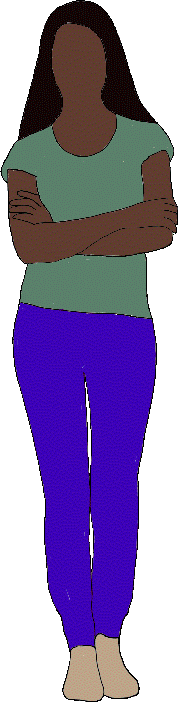
\includegraphics[width=0.04\textwidth]{figures/Relativity/woman_standing}};
}
{
\node[above=-0.5cm] at (-0.01*\L,0) {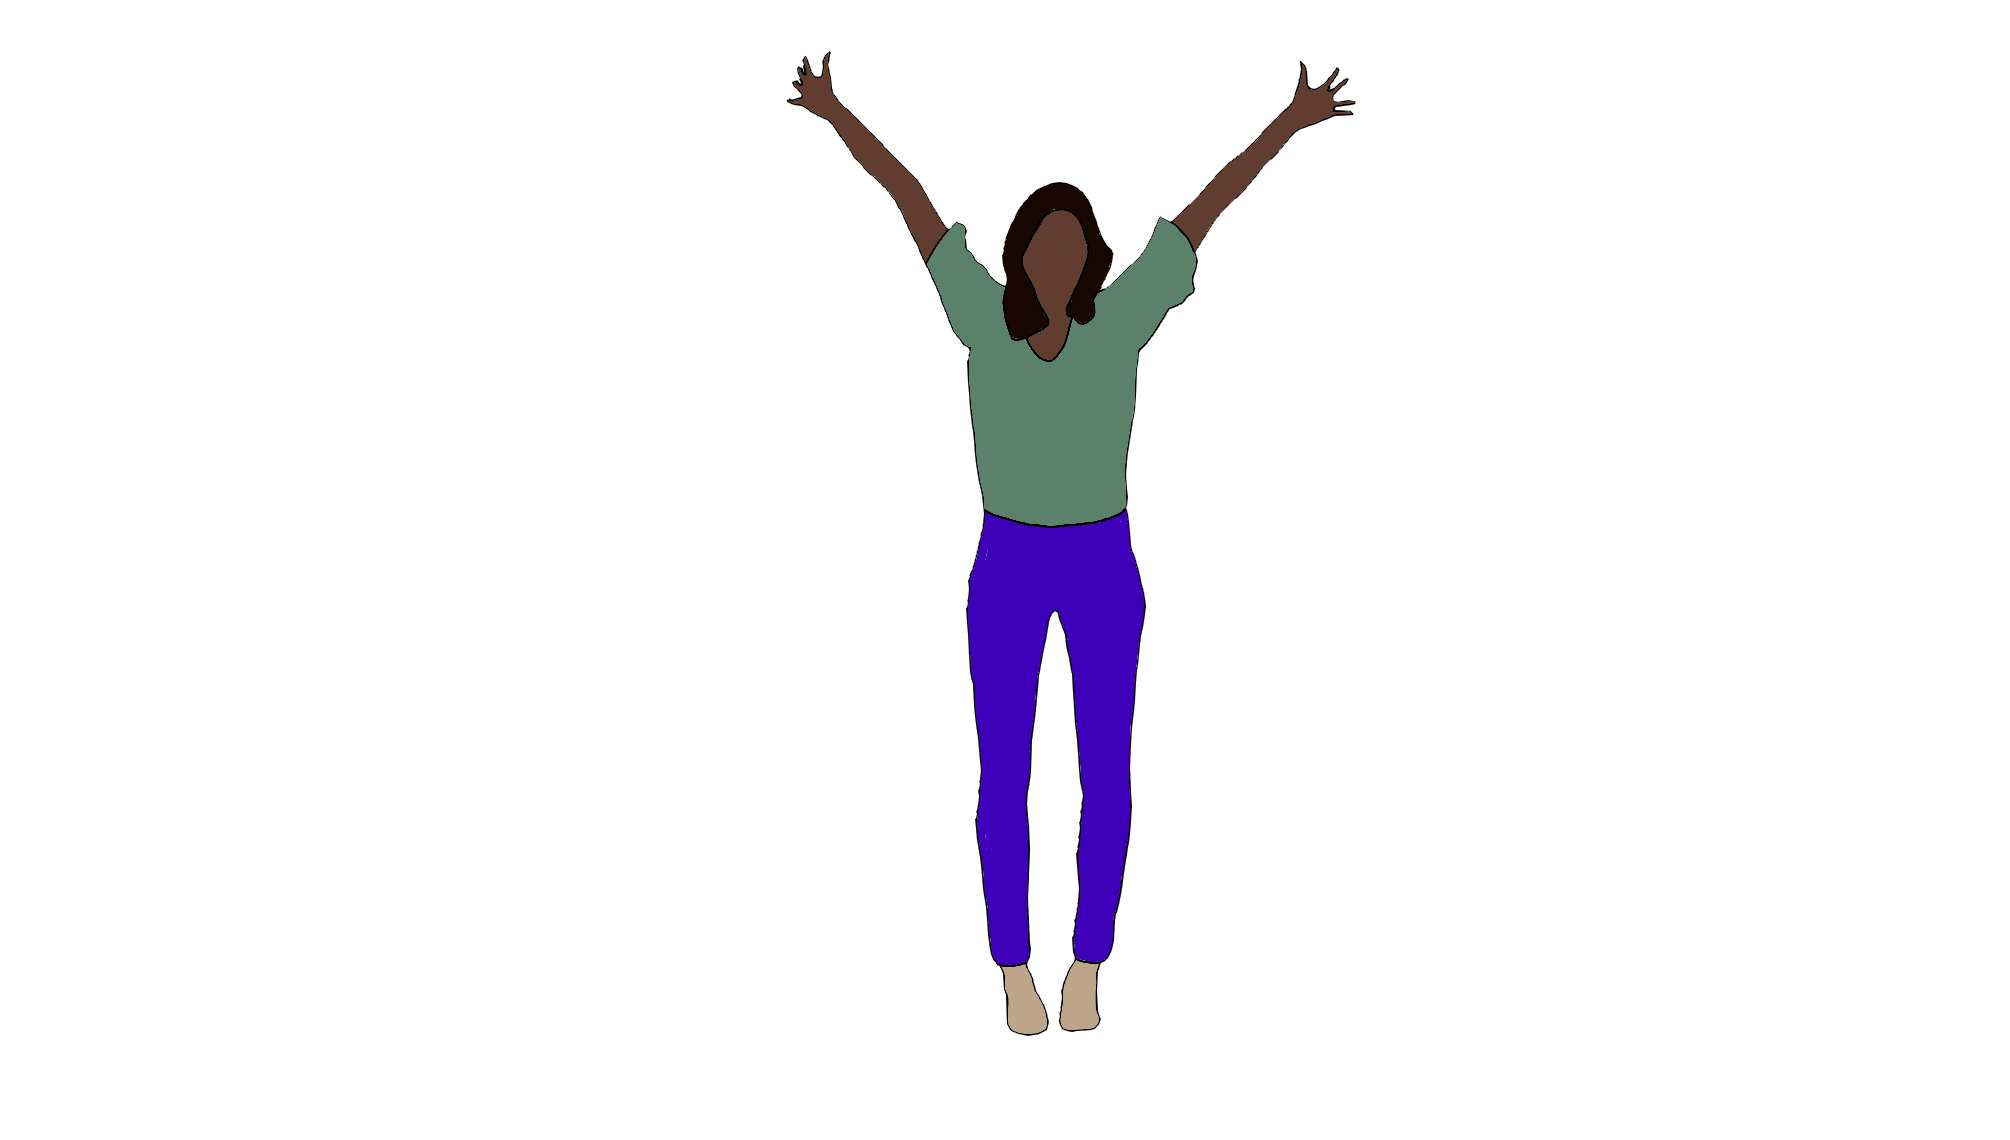
\includegraphics[width=0.4\textwidth]{figures/Relativity/alice_arms_png}};
}


\ifthenelse{\i<6}{
\node[above=-0.2cm] at (-0.4*\L,\h) {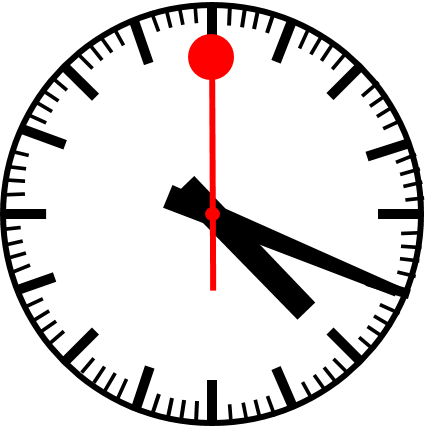
\includegraphics[width=0.07\textwidth]{figures/Relativity/fourtwenty.png}};
}{}
\ifthenelse{\i>5 \AND \i<12}{
\node[above=-0.2cm] at (-0.4*\L,\h) {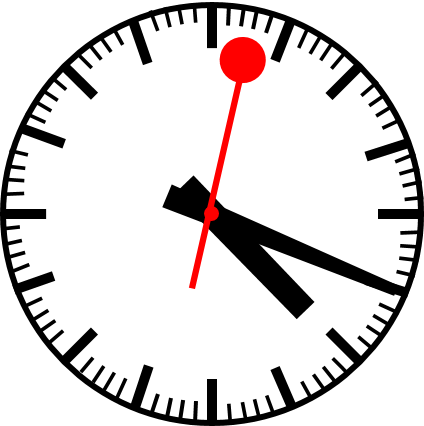
\includegraphics[width=0.07\textwidth]{figures/Relativity/fourtwenty_1.png}};
}{}
\ifthenelse{\i>11 \AND \i<18}{
\node[above=-0.2cm] at (-0.4*\L,\h) {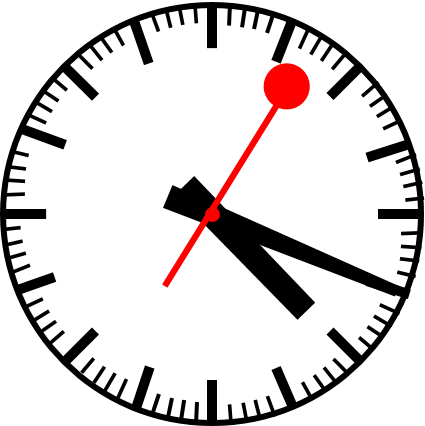
\includegraphics[width=0.07\textwidth]{figures/Relativity/fourtwenty_2.png}};
}{}
\ifthenelse{\i>17}{
\node[above=-0.2cm] at (-0.4*\L,\h) {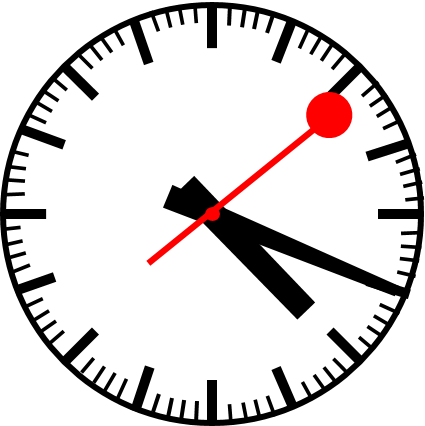
\includegraphics[width=0.07\textwidth]{figures/Relativity/fourtwenty_3.png}};
}{}

\ifthenelse{\i<6}{
\node[above=-0.2cm] at (0.4*\L,\h) {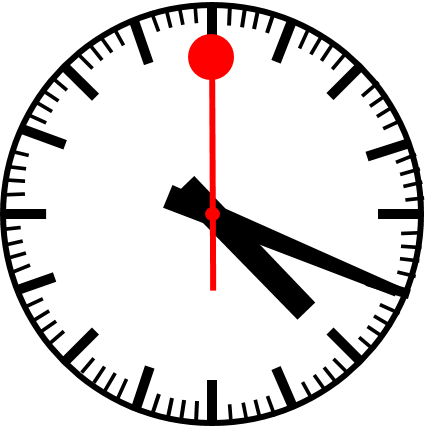
\includegraphics[width=0.07\textwidth]{figures/Relativity/fourtwenty.png}};
}{}
\ifthenelse{\i>5 \AND \i<12}{
\node[above=-0.2cm] at (0.4*\L,\h) {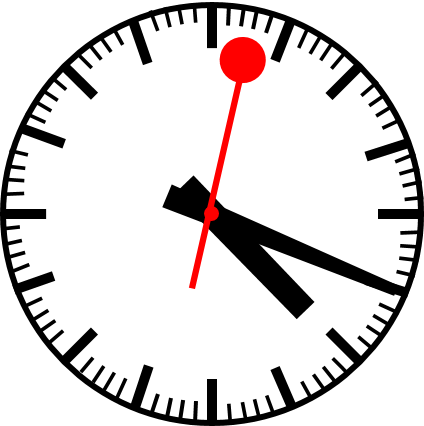
\includegraphics[width=0.07\textwidth]{figures/Relativity/fourtwenty_1.png}};
}{}
\ifthenelse{\i>11 \AND \i<18}{
\node[above=-0.2cm] at (0.4*\L,\h) {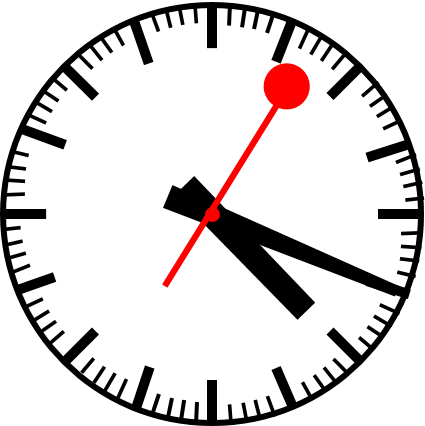
\includegraphics[width=0.07\textwidth]{figures/Relativity/fourtwenty_2.png}};
}{}
\ifthenelse{\i>17}{
\node[above=-0.2cm] at (0.4*\L,\h) {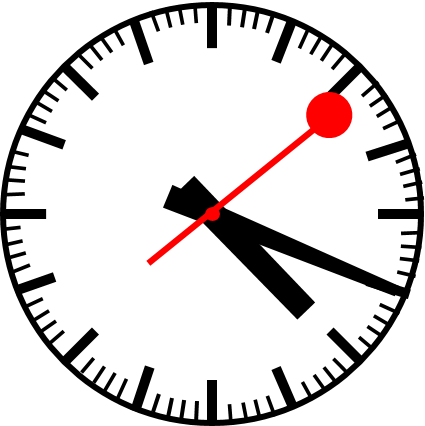
\includegraphics[width=0.07\textwidth]{figures/Relativity/fourtwenty_3.png}};
}{}

\end{tikzpicture}
}%multiframe
\end{animateinline}


\begin{itemize}
\item An observer on a platform is equidistant from 2 clocks that output pulses of light. When the clocks read 16:20, they output a light pulse, the observer sees the two light pulses at the same time and she concludes that the clock are synchronized.
\end{itemize}

\end{frame}



%% Simultaneity Animation 2
%%%%%%%%%%%%%%%%%%%%%%%%%%%%%%
\begin{frame}{Simultaneity}

\centering

\pgfmathtruncatemacro\N{24}
\begin{animateinline}[autoplay,loop]{4} % 5 fps, same as 0.2 s transduration

\multiframe{\N}{i=0+1}{

\tikzmath{
%\i=1;
\L=10;
\w=0.2;%thickness of platform
\h=2;
\D=0.3*\L;
\xs=0.25*\L-\i*0.5*\L/\N;%platform shift
\xr=\xs+0.33*\L-\i*\D/\N;%position of right laser
\xl=-\xs+0.33*\L+\i*\D/\N-1.12*\L;%position of left laser
}
\begin{tikzpicture}

\useasboundingbox (-0.7*\L,-\h) rectangle (0.7*\L,1.5*\h);


%moving platform
\begin{scope}[shift={(\xs,0)}]
%platform
\fill[color=black!70] (-\L/2,-\w) rectangle (\L/2,0);
%posts
\fill[color=qblue!70] (-0.42*\L,0) rectangle (-0.38*\L,0.97*\h);
\fill[color=qblue!70] (0.38*\L,0) rectangle (0.42*\L,0.97*\h);
\ifthenelse{\i<23}{
\node[above=-0.2cm] at (0,0) {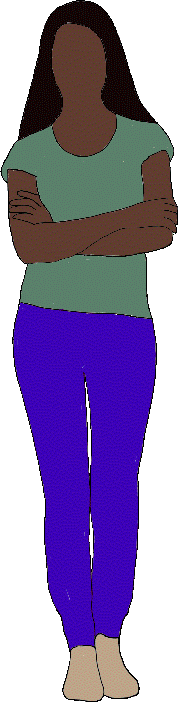
\includegraphics[width=0.04\textwidth]{figures/Relativity/woman_standing}};
}
{
\node[above=-0.5cm] at (-0.01*\L,0) {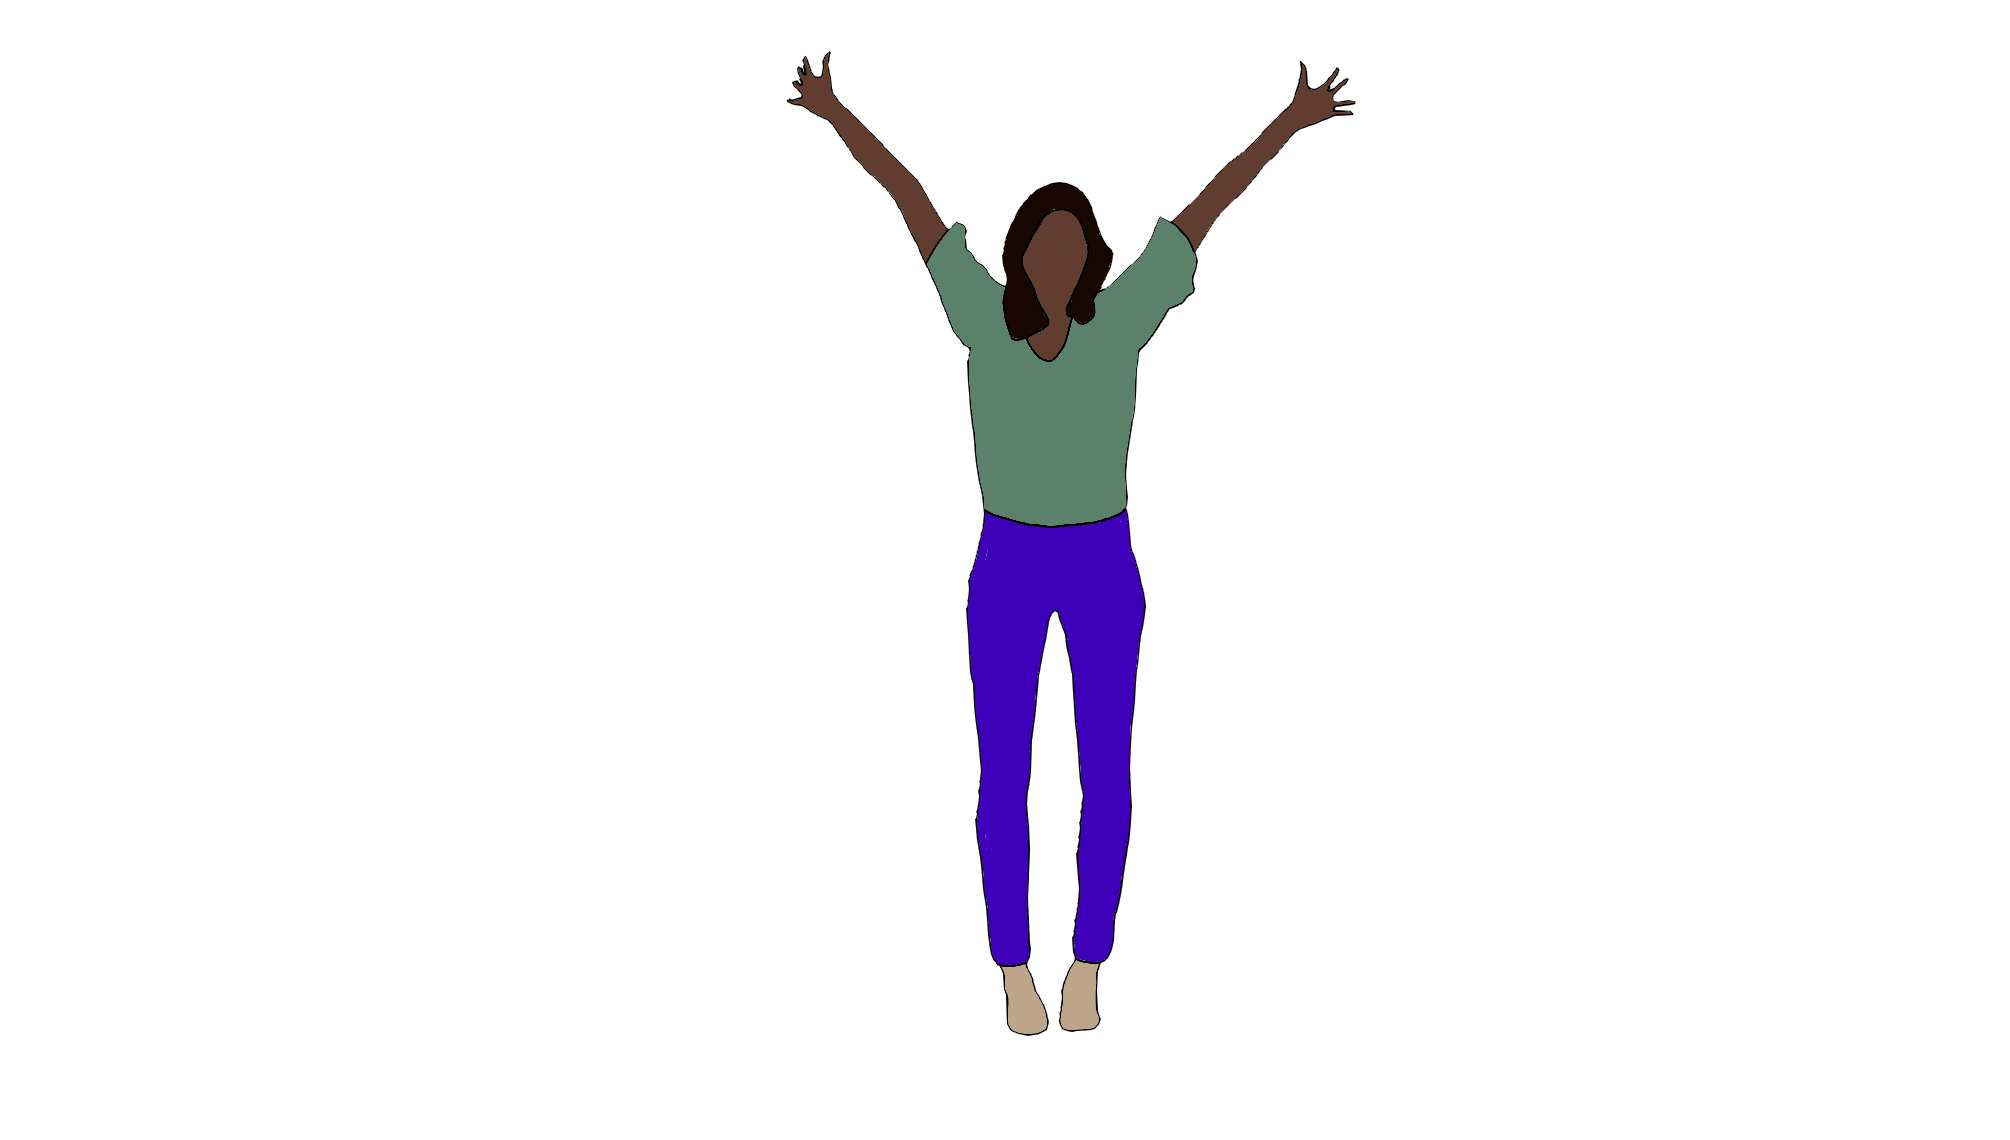
\includegraphics[width=0.4\textwidth]{figures/Relativity/alice_arms_png}};
}

%left clock
\ifthenelse{\i<5}{
\node[above=-0.2cm] at (-0.4*\L,\h) {
\includegraphics[width=0.07\textwidth]{figures/Relativity/fourtwenty_m3.png}};
}{}
\ifthenelse{\i>4 \AND \i<11}{
\node[above=-0.2cm] at (-0.4*\L,\h) {
\includegraphics[width=0.07\textwidth]{figures/Relativity/fourtwenty_m2.png}};
}{}
\ifthenelse{\i>10 \AND \i<17}{
\node[above=-0.2cm] at (-0.4*\L,\h) {
\includegraphics[width=0.07\textwidth]{figures/Relativity/fourtwenty_m1.png}};
}{}
\ifthenelse{\i>16}{
\node[above=-0.2cm] at (-0.4*\L,\h) {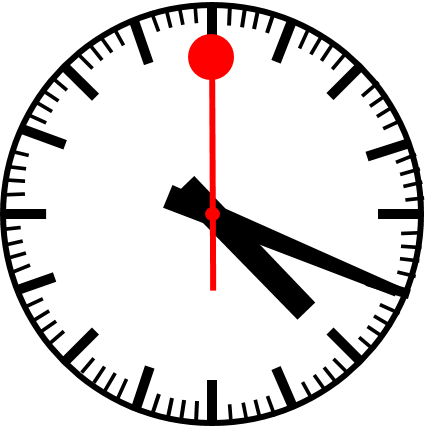
\includegraphics[width=0.07\textwidth]{figures/Relativity/fourtwenty.png}};
}{}


%right clock
\ifthenelse{\i<5}{
\node[above=-0.2cm] at (0.4*\L,\h) {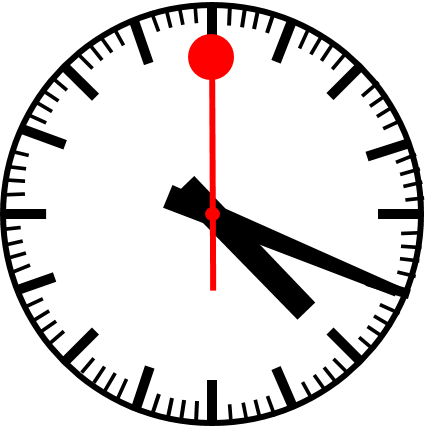
\includegraphics[width=0.07\textwidth]{figures/Relativity/fourtwenty.png}};
}{}
\ifthenelse{\i>4 \AND \i<11}{
\node[above=-0.2cm] at (0.4*\L,\h) {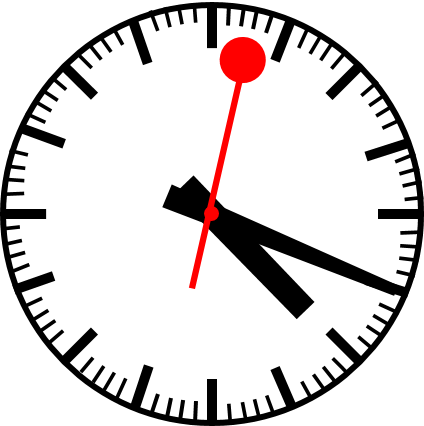
\includegraphics[width=0.07\textwidth]{figures/Relativity/fourtwenty_1.png}};
}{}
\ifthenelse{\i>10 \AND \i<17}{
\node[above=-0.2cm] at (0.4*\L,\h) {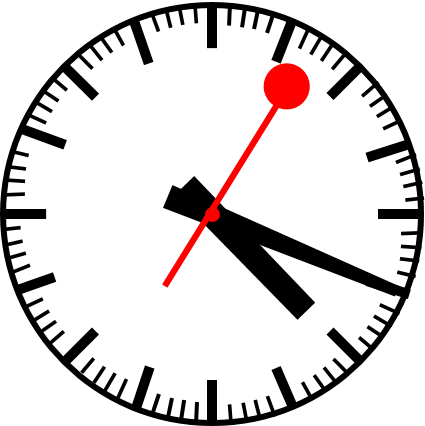
\includegraphics[width=0.07\textwidth]{figures/Relativity/fourtwenty_2.png}};
}{}
\ifthenelse{\i>16}{
\node[above=-0.2cm] at (0.4*\L,\h) {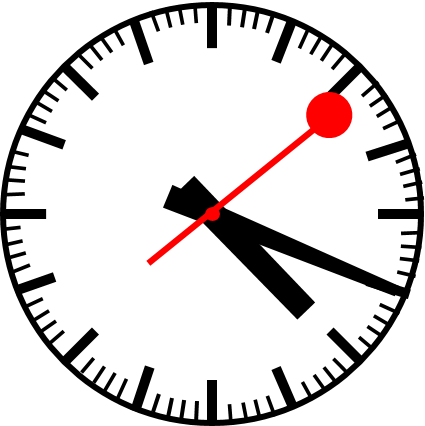
\includegraphics[width=0.07\textwidth]{figures/Relativity/fourtwenty_3.png}};
}{}

\end{scope}

%foreground person
\node[above=-0.5cm] at (-0.5*\L,-0.5*\h) {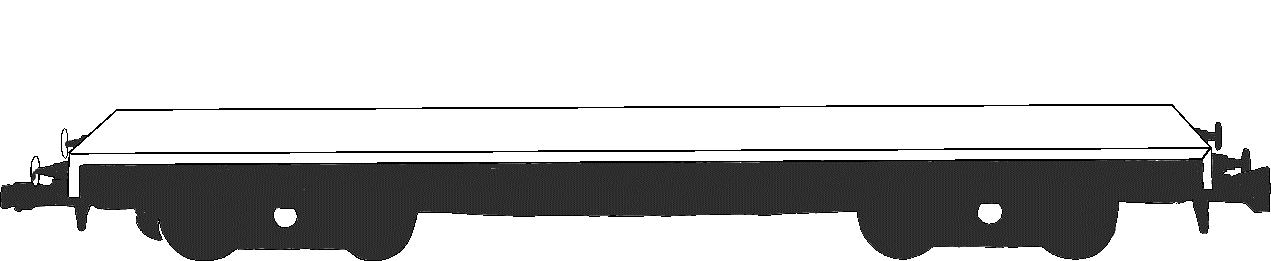
\includegraphics[width=0.4\textwidth]{figures/Relativity/traincart}};
\node[above=0cm] at (-0.5*\L,-0.5*\h) {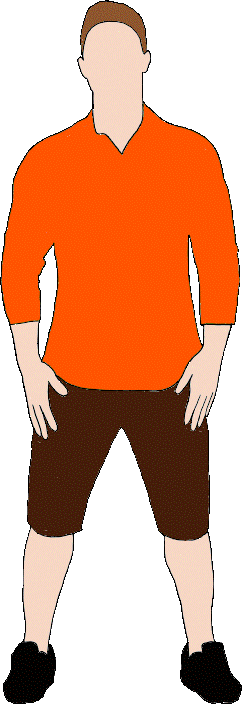
\includegraphics[width=0.06\textwidth]{figures/Relativity/man_standing_ink}};


%laser ball
\draw [color=qred, line width =1.5pt] (\xr,1.2*\h) -- (0.6*\L,1.2*\h);
\node [color=qred, star, star points=10, star point height=.1cm, minimum size=0.2cm, fill] at(\xr,1.2*\h) {};
\ifthenelse{\i>16}{
\draw [color=qred, line width =1.5pt] (\xl,1.2*\h) -- (-0.5*\L,1.2*\h);
\node [color=qred, star, star points=10, star point height=.1cm, minimum size=0.2cm, fill] at(\xl,1.2*\h) {};
}{}

\end{tikzpicture}
}%multiframe
\end{animateinline}

\begin{itemize}
\item An observer on a train sees the platform moving in his rest frame. He observes two pulses of light arrive at the same time at the person on the platform. 
\item He concludes that the pulse from the right happened first, since the pulses travel at speed $c$ and the one from the right travelled further. He disagrees that the clocks are synchronized! \textbf{But, causality...}
\end{itemize}

\end{frame}



%%%%%%%%%%%%%%%%%%%%%%%%%%%%%%
\begin{bulletframe}{Defining ``events'' and frames of reference}
\item We considered the ``event'': \emph{``The person on the platform received two pulses of light at the same time.''}
\item We did not consider the ``event'': \emph{``The two clocks emitted a pulse of light at the same time.''}
\item This led to the conclusion that simultaneity is relative:
\begin{itemize}
\item The second statement is not an ``event'' because the two clocks are at different positions in space. 
\item[$\rightarrow$] We can only compare things that happen at the same location in space and time. An ``event'' is something that occurs at a single location in space and time.
\item[$\rightarrow$] We introduce ``space-time'', and we say that an event is something that happens in four-dimensional space-time and has coordinates (x,y,z,t)
\item[$\rightarrow$] We can then compare if events in space-time are simultaneous or not:
\begin{itemize}
\item[$\rightarrow$] ''Person receiving two pulses of light'' is always after ``clock A'' and  ``clock B'' emit a pulse of light. You can check this out; the only way for this not to be true is if one of the observers goes faster than c.
\item[$\rightarrow$] ``clock A emits a pulse of light'' is not always at the same time as ``clock B emits a pulse of light''. We just showed that it can be before or after as well!
\end{itemize}
\end{itemize}

\end{bulletframe}


%%%%%%%%%%%%%%%%%%%%%%%%%%%%%%



%%%%%%%%%%%%%%%%%%%%%%%%%%%%%%
\subsection{Example question}
\label{subsec:examplequestion}
\twocolframesf{Example question}
{
\begin{itemize}
\item Repulsive force per unit length between two charged wires:
\begin{align*}
\frac{F^E_0}{l}=\frac{\lambda_0}{2\pi \epsilon_0 r}
\end{align*}
\item Attractive force per unit length between two current carrying wires:
\begin{align*}
\frac{F^B_0}{l}=\frac{\mu_0 I^2}{2\pi r}
\end{align*}
\end{itemize}
}
{
\centering
\begin{tikzpicture}
\tikzmath{
\r=0.75;
\L=2.5;
\Np=6;
}
%top part:
%\wires
\draw[line width=1.5] (-\r/2,-\L/2) -- (-\r/2,\L/2) node[above,color=qred] {$\lambda_0$};
\draw[line width=1.5] (\r/2,-\L/2) -- (\r/2,\L/2) node[above,color=qred] {$\lambda_0$};
%charges
\foreach \i in {0,...,\Np}{
 \tikzmath{
   \yp=-\L/2+\i*\L/\Np;
 }
 \node[color=qred] at (-\r/2,\yp) {\small \textbf{+}};
 \node[color=qred] at (\r/2,\yp) {\small \textbf{+}};
}
%labels
\draw[latex-latex] (-\r/2,0) -- (\r/2,0) node[midway,above]{$r$};

\begin{scope}[shift={(0,-1.5*\L)}]
%\wires
\draw[line width=1.5] (-\r/2,-\L/2) -- (-\r/2,\L/2) ;
\draw[line width=1.5] (\r/2,-\L/2) -- (\r/2,\L/2) ;
%current
\draw[line width=1.5, color=qred,-latex] (-\r/2,-0.2*\L) -- (-\r/2,0.2*\L) node[left]{$I$};
\draw[line width=1.5, color=qred,-latex] (\r/2,-0.2*\L) -- (\r/2,0.2*\L) node[right]{$I$};
%labels
\draw[latex-latex] (-\r/2,0) -- (\r/2,0) node[midway,above]{$r$};
\end{scope}
\end{tikzpicture}

}

%%%%%%%%%%%%%%%%%%%%%%%%%%%%%%
\twocolframesf{Example question}
{
\only<1>{
\begin{itemize}
\item In a frame moving downwards with speed $v$, it looks like there is an upwards current given by:
\begin{align*}
I=\frac{dQ}{dt}=\frac{d(\lambda l)}{dt}=\lambda v
\end{align*}
\item \textbf{Let us assume that the laws of physics and that the constants of nature remain the same in this frame of reference}. The force on one of the wires must remain the same:
\begin{align*}
\frac{F^E_0}{l}=\frac{\textcolor{qred}{\lambda_0}}{2\pi \epsilon_0 r}=\frac{\textcolor{qred}{\lambda}}{2\pi \epsilon_0 r}-\frac{\mu_0 I^2}{2\pi r}
\end{align*}
\end{itemize}
Charge density is the only thing that can be different in the moving frame, so we call it $\textcolor{qred}{\lambda}$. 
}
\only<2>{
Working through the math:
\begin{align*}
\frac{\lambda_0}{2\pi \epsilon_0 r}&=\frac{\lambda}{2\pi \epsilon_0 r}-\frac{\mu_0 (\lambda v)^2}{2\pi r}\\
\frac{\lambda_0}{\epsilon_0 r}&=\frac{\lambda}{\epsilon_0}-\mu_0 (\lambda v)^2\\
\lambda_0^2&=\lambda^2(1-\epsilon_0\mu_0v^2)\\
\therefore \lambda &= \lambda_0 \frac{1}{\sqrt{1-\epsilon_0\mu_0v^2}}\\
\Aboxed{\therefore \lambda &=\lambda_0 \frac{1}{\sqrt{1-\frac{v^2}{c^2}}}}
\end{align*}
From Maxwell's equations: $c=\frac{1}{\sqrt{\epsilon_0\mu_0}}$
}
\only<3>{
The charge density \emph{is} different in the moving frame of reference (and larger since $v < c$):
\begin{align*}
\lambda &=\lambda_0 \frac{1}{\sqrt{1-\frac{v^2}{c^2}}}
\end{align*}
\begin{itemize}
\item Observers in the two reference frames can agree on the number of charges in a section of wire (they could literally count the charges between 2 lines drawn on the wire). 
\item The only way for the charge density to be higher in the moving reference frame is if \textbf{the wire is actually shorter (the lines are closer)!}
\end{itemize}
}
}
{
\centering
\pgfmathtruncatemacro\N{10}
\begin{animateinline}[autoplay,loop]{4} % 5 fps, same as 0.2 s transduration
\multiframe{\N}{i=0+1}{

\begin{tikzpicture}
\tikzmath{
\r=0.75;
\L=5.;
\Np=12;
\Npp=12;
\dy=\i*\L/\Npp/\N;
}
\only<3>{
\tikzmath{
\Npp=18;
\dy=\i*\L/\Npp/\N;
}
}

%first wire pair
%\wires
\draw[line width=1.5] (-\r/2,-\L/2) -- (-\r/2,\L/2) node[above,color=qred] {$\lambda_0$};
\draw[line width=1.5] (\r/2,-\L/2) -- (\r/2,\L/2) node[above,color=qred] {$\lambda_0$};
%charges
\foreach \iy in {0,...,\Np}{
 \tikzmath{
   \yp=-\L/2+\iy*\L/\Np;
 }
 \node[color=qred] at (-\r/2,\yp) {\small \textbf{+}};
 \node[color=qred] at (\r/2,\yp) {\small \textbf{+}};
}
%labels
\draw[latex-latex] (-\r/2,0) -- (\r/2,0) node[midway,above]{$r$};
\only<3>{
\draw[line width=2, color=qblue!70] (-0.6*\r,0.25*\L) -- (0.6*\r,0.25*\L);
\draw[line width=2, color=qblue!70] (-0.6*\r,-0.25*\L) -- (0.6*\r,-0.25*\L);
}


%second wire
\begin{scope}[shift={(3*\r,0)}]
%\wires
\draw[line width=1.5] (-\r/2,-\L/2) -- (-\r/2,\L/2) node[above,color=qred] {$\lambda$};
\draw[line width=1.5] (\r/2,-\L/2) -- (\r/2,\L/2) node[above,color=qred] {$\lambda$};
%charges
\foreach \iy in {1,...,\Npp}{
 \tikzmath{
   \yp=-\L/2+(\iy-1)*\L/\Npp+\dy;
 }
 \node[color=qred] at (-\r/2,\yp) {\small \textbf{+}};
 \node[color=qred] at (\r/2,\yp) {\small \textbf{+}};
 }
%current
\draw[line width=1.5, color=qred,-latex] (-0.8*\r,-0.2*\L) -- (-0.8*\r,0.2*\L) node[left]{$I$};
\draw[line width=1.5, color=qred,-latex] (0.8*\r,-0.2*\L) -- (0.8*\r,0.2*\L) node[right]{$I$};
\only<3>{
\draw[line width=2, color=qblue!70] (-0.6*\r,0.25*\L*\Np/\Npp) -- (0.6*\r,0.25*\L*\Np/\Npp);
\draw[line width=2, color=qblue!70] (-0.6*\r,-0.25*\L*\Np/\Npp) -- (0.6*\r,-0.25*\L*\Np/\Npp);
}
%labels
\draw[latex-latex] (-\r/2,0) -- (\r/2,0) node[midway,above]{$r$};
\end{scope}
\end{tikzpicture}
}%multiframe
\end{animateinline}
\captionof*{figure}{\textit{Two charged wires viewed at rest (left) and from a frame of reference that is moving downwards (right).}}
}


%%%%%%%%%%%%%%%%%%%%%%%%%%%%%%
\subsection{Length contraction}
\label{subsec:lengthcontraction}
\twocolframesf{Length contraction}
{
\begin{itemize}
\item An object that is moving is shorter in the direction of motion than you would measure if the object were at rest.
\item This is real, stuff shrinks lengthwise as it moves fast.
\begin{align*}
L=L_0\sqrt{1-\frac{v^2}{c^2}}<L_0
\end{align*}
\end{itemize}
}
{
\centering
\begin{tikzpicture}
\begin{scope}
\clip(-2,-2) rectangle (2.2,2);
\node at (0,-1) {
\includegraphics[width=0.8\textwidth, height=0.3\textwidth]{figures/Relativity/qtrain}};
\node at (0,1) {
\includegraphics[width=1\textwidth, height=0.3\textwidth]{figures/Relativity/qtrain}};
\end{scope}

\draw[latex-latex] (-1.6,2) -- (1.9,2)node[midway,above]{$L_0$};
\draw[latex-latex] (-1.2,-1.8) -- (1.7,-1.8)node[midway,below]{$L$};

\end{tikzpicture}
}

%%%%%%%%%%%%%%%%%%%%%%%%%%%%%%
%%%%%%%%%%%%%%%%%5should animate (doesn work?)
%%%%%%%%%%%%%%%%%%%%%%%%%%%%%%
\subsection{Special relativity and E/M}
\label{subsec:speacialrelativityandem}
\twocolframesf{Special Relativity and E/M}
{
\begin{itemize}
\item A (neutral) wire carries current (electrons moving to the right relative to stationary ions).
\item We place a charge $+Q$ near the wire, it feels no net force. 
\item We would say the current creates a magnetic field out of the page, but since $Q$ is not moving, it feels no force ($\vec F=Q \vec v \times \vec B$).
\item<2> If $Q$ moved towards the right, it would feel a downward magnetic force.
\end{itemize}
}
{
\centering
\pgfmathtruncatemacro\N{10}
\begin{animateinline}[autoplay,loop]{4} % 5 fps, same as 0.2 s transduration
\multiframe{\N}{i=0+1}{
\begin{tikzpicture}
\tikzmath{
\L=4.5;
\r=1.2;
\h=1.5*\r;
\Np=10;
\Ne=10;
\dy=\i*\L/\Ne/\N;
}
%\useasboundingbox (-0.7*\L,-2*\r) rectangle (0.7*\L,1.2*\r);
\draw[opacity=0] (-0.7*\L,-3*\r) rectangle (0.6*\L,1.2*\r);
%wire
\fill[color=black!70,opacity=0.8] (-\L/2,-\r/2) rectangle (\L/2,\r/2) ;
%electrons and ions
\foreach \ip in {1,...,\Np}{
  \tikzmath{
   \xp=-\L/2+\ip*\L/\Np-0.5*\L/\Np;
  }
 \fill[color=qblue] (\xp,0.2*\r) circle (5pt);
 \node[color=white] at (\xp,0.2*\r) {+};
}
\begin{scope}%cut the charges exiting the edge...
\clip (-\L/2,-\r/2) rectangle (\L/2,\r/2) ;
\foreach \ip in {1,...,\Ne}{
  \tikzmath{
   \xe=-\L/2+(\ip-1)*\L/\Ne+\dy;
  }
 \fill[color=qred] (\xe,-0.2*\r) circle (3pt);
 \node[text=white] at (\xe,-0.2*\r) {-};
}
\end{scope}
%charge
\fill[color=qblue] (0,-\h) circle (3pt);
\node[left,color=qblue] at (0,-\h) {$+Q$};
\only<2>{
\draw[-latex, line width=1.5] (0,-\h) -- +(1,0) node[right]{$\vec v$};
\draw[-latex, line width=1.5] (0,-\h) -- +(0,-1) node[left]{$\vec F_B$};
}


%Labels
\node[left,color=qblue] at (-0.2*\L,-\h) {$\vec B\;\odot$};
\draw[-latex, line width=1.5] (0.1*\L,0.75*\r) -- (-0.1*\L,0.75*\r) node[midway,above]{$I$};
\draw[latex-, line width=1.5, color=qred] (0.1*\L,-0.75*\r) -- (-0.1*\L,-0.75*\r) node[midway,below]{$\vec v_d$};

\end{tikzpicture}
}%multiframe
\end{animateinline}
\captionof*{figure}{\textit{In the reference frame of the wire: A charge is near a wire with current. The charge feels a magnetic force if it moves relative to the wire.}}
}

%%%%%%%%%%%%%%%%%%%%%%%%%%%%%%
%%%%%%%%%shoujld animate as well, also doesn't  work
%%%%%%%%%%%%%%%%%%%%%%%%%%%%%%
\twocolframesf{Special Relativity and E/M}
{
Suppose that $Q$ moves to the right, \emph{with the same speed as the electrons}. \textbf{In the frame of $Q$}:
\begin{itemize}
\item<2-> The electrons are immobile and \emph{are sparse} (they were length contracted).
\item<2-> The ions move to the left and \emph{are denser} (they are length contracted).
\item<3->[$\rightarrow$] The wire no longer appears neutral and repels $Q$ by the \textbf{electric force}, which must have the same magnitude.
\item<3->[$\rightarrow$] Since $Q$ is stationary, there is no force from the magnetic field due to the moving ions.
\item<3->[$\rightarrow$] The magnetic and electric force are really different aspects of the same effect, Special Relativity is the connection!
\end{itemize}
}
{
\centering
\pgfmathtruncatemacro\N{10}
\begin{animateinline}[autoplay,loop]{4} % 5 fps, same as 0.2 s transduration
\multiframe{\N}{i=0+1}{
\begin{tikzpicture}
\tikzmath{
\L=4.5;
\r=1.2;
\h=1.5*\r;
\Np=12;
\Ne=7;
\dy=\i*\L/\Np/\N;
}
%\useasboundingbox (-0.7*\L,-2*\r) rectangle (0.7*\L,1.2*\r);
\draw[opacity=0] (-0.7*\L,-3*\r) rectangle (0.6*\L,1.2*\r);
%wire
\fill[color=black!70,opacity=0.8] (-\L/2,-\r/2) rectangle (\L/2,\r/2) ;
%electrons and ions
\begin{scope}%cut the charges exiting the edge...
\clip (-\L/2,-\r/2) rectangle (\L/2,\r/2) ;
\foreach \ip in {1,...,\Np}{
  \tikzmath{
   \xp=-\L/2+(\ip)*\L/\Np-\dy;
  }
 \fill[color=qblue] (\xp,0.2*\r) circle (5pt);
 \node[color=white] at (\xp,0.2*\r) {+};
}
\end{scope}
\foreach \ip in {1,...,\Ne}{
  \tikzmath{
   \xe=-\L/2+\ip*\L/\Ne-0.5*\L/\Ne;
  }
 \fill[color=qred] (\xe,-0.2*\r) circle (3pt);
 \node[text=white] at (\xe,-0.2*\r) {-};
}

%charge
\fill[color=qblue] (0,-\h) circle (3pt);
\node[left,color=qblue] at (0,-\h) {$+Q$};
\only<3->{
\draw[-latex, line width=1.5] (0,-\h) -- +(0,-1) node[left]{$\vec F_E$};
}
%Labels
\node[left,color=qblue] at (-0.2*\L,-\h) {$\vec B'\;\odot$};
\draw[-latex, line width=1.5] (0.1*\L,0.75*\r) -- (-0.1*\L,0.75*\r) node[midway,above]{$I'$};

\end{tikzpicture}
}%multiframe
\end{animateinline}
\only<1-2>{
\captionof*{figure}{\textit{In the reference frame of the charge moving with the electrons.}}
}
\only<3>{
\captionof*{figure}{\textit{In the reference frame of the charge moving with the electrons. It feels a purely electric force due to the apparent net charge on the wire.}}
}
}

%%%%%%%%%%%%%%%%%%%%%%%%%%%%%%
\subsection{Einstein's Clock}
\label{subsec:einsteinsclock}
\twocolframesf{Einstein's Clock}
{
\begin{itemize}
\item A beam of light bounces back and forth between 2 mirrors.
\item You watch the light beam, and determine that the time for a return trip of the light is:
\begin{align*}
\Delta \tau = \frac{2D}{c}
\end{align*}
\end{itemize}
The speed of light is:
\begin{align*}
c= \frac{2D}{\tau}
\end{align*}
Note: You measure the time difference between two events at the same position, as far as you are concerned.
}
{
\centering
\begin{tikzpicture}
\tikzmath{
\D=3;
\L=5;
}
\fill[draw=black,color=qblue!60,opacity=0.7] (0,-\D/2) -- (0,\D/2) -- (\L/2,\D/2) -- (0.75*\L,0) --  (\L/2,-\D/2) -- (0,-\D/2);

\node [color=qred, star, star points=10, star point height=.1cm, minimum size=0.2cm, fill] at (0.075*\L,-0.4*\D) {};
\draw[color=qred,line width=1.5,dashed] (0.1*\L,-0.4*\D) -- (0.25*\L,0.5*\D); 
\draw[color=qred,line width=1.5,dashed]  (0.25*\L,0.5*\D) -- (0.4*\L,-0.4*\D); 
\fill (0.35*\L,-0.5*\D) rectangle (0.45*\L,-0.4*\D);
\draw[latex-latex] (-0.05*\L,-\D/2) -- (-0.05*\L,\D/2) node[midway, left] {$D$};

\end{tikzpicture}
\captionof*{figure}{\textit{A beam of light can be used as a clock in this spaceship. Here the path of the beam is viewed in the reference frame of the spaceship.}}
}



%%%%%%%%%%%%%%%%%%%%%%%%%%%%%%
\twocolframesf{Einstein's Clock}
{
\begin{itemize}
\item You take your clock on a spaceship and someone on Earth observes the light beam.
\item The light travels a longer distance as far as they are concerned, but the speed of the light beam is still $c$ (in the diagonal direction in the above diagram).
\item They measure the time difference between events that happen at different locations.
\item They would write the speed of light as:
\begin{align*}
c= \frac{2\sqrt{D^2+l^2}}{\Delta t}=\frac{2\sqrt{D^2+\left(\frac{v\Delta t}{2} \right)^2}}{\Delta t}
\end{align*}
\end{itemize}
}
{
\centering
\begin{tikzpicture}
\tikzmath{
\D=3;
\L=4.5;
\fss=0.4;
}
\begin{scope}[shift={(-0.4*\L,0)}, scale=\fss, opacity=0.2]
\fill[draw=black, dashed,color=qblue!60,opacity=0.7] (0,-\D/2) -- (0,\D/2) -- (\L/2,\D/2) -- (0.75*\L,0) --  (\L/2,-\D/2) -- (0,-\D/2);
\node [color=qred, star, star points=10, fill] at (0.075*\L,-0.4*\D) {};
\fill (0.35*\L,-0.5*\D) rectangle (0.45*\L,-0.4*\D);
\end{scope}

\begin{scope}[shift={(0,0)}, scale=\fss, opacity=0.2]
\fill[draw=black, dashed, color=qblue!60,opacity=0.7] (0,-\D/2) -- (0,\D/2) -- (\L/2,\D/2) -- (0.75*\L,0) --  (\L/2,-\D/2) -- (0,-\D/2);
\node [color=qred, star, star points=10, fill] at (0.075*\L,-0.4*\D) {};
\fill (0.35*\L,-0.5*\D) rectangle (0.45*\L,-0.4*\D);
\end{scope}

\begin{scope}[shift={(0.4*\L,0)}, scale=\fss]
\fill[color=qblue!60,opacity=0.7] (0,-\D/2) -- (0,\D/2) -- (\L/2,\D/2) -- (0.75*\L,0) --  (\L/2,-\D/2) -- (0,-\D/2);
\node [draw=black,color=qred, star, star points=10, fill, opacity=0.5] at (0.075*\L,-0.4*\D) {};
\fill (0.35*\L,-0.5*\D) rectangle (0.45*\L,-0.4*\D);
\end{scope}

%light ray
\draw[color=qred,line width=1.5,dashed] (-0.4*\L+\fss *0.1*\L,-\fss*0.4*\D) -- (\fss*0.25*\L,\fss*0.5*\D); 
\draw[color=qred,line width=1.5,dashed]  (\fss*0.25*\L,\fss*0.5*\D) -- (0.4*\L+\fss*0.4*\L,-\fss*0.4*\D); 
%labels
\draw[latex-latex] (-0.45*\L,-\fss*\D/2) -- (-0.45*\L,\fss*\D/2) node[midway, left] {$D$};
\draw[latex-latex] (-0.4*\L,\fss*1.2*\D/2) -- (\fss*0.25*\L,\fss*1.2*\D/2) node[midway, above] {$l$};
\draw[latex-latex] (\fss*0.25*\L,\fss*1.2*\D/2) -- (0.4*\L+\fss*0.4*\L,\fss*1.2*\D/2) node[midway, above] {$l$};

\end{tikzpicture}
\captionof*{figure}{\textit{A beam of light can be used as a clock in this spaceship. Here, the path of the beam is viewed by someone on Earth, as the spaceship moves to the right with speed, $v$.}}
\only<2>{
Re-arranging to isolate time, $\Delta t$:
\begin{align*}
\Delta t = \frac{2D}{c\sqrt{1-\frac{v^2}{c^2}}}=\frac{\Delta \tau}{\sqrt{1-\frac{v^2}{c^2}}}
\end{align*}
}
}

%%%%%%%%%%%%%%%%%%%%%%%%%%%%%%
\subsection{The gamma factor}
\label{subsec:thegammafactor}
\begin{frame}{Gamma}
\begin{itemize}
\item The factor:
\begin{align*}
\gamma = \frac{1}{\sqrt{1-\frac{v^2}{c^2}}}
\end{align*}
\end{itemize}
comes up a lot, so we call it $\gamma$. $v$ is the relative speed between two observers in inertial frames of reference. 
\end{frame}


%%%%%%%%%%%%%%%%%%%%%%%%%%%%%%



%%%%%%%%%%%%%%%%%%%%%%%%%%%%%%
\subsection{Time dilation}
\label{subsec:timedilation}
\begin{frame}{Time dilation}
\begin{align*}
\Delta t = \gamma \Delta \tau = \frac{1}{\sqrt{1-\frac{v^2}{c^2}}} \Delta\tau
\end{align*}
\begin{itemize}
\item The \textbf{``proper time''}, $\Delta\tau$, is the time that someone measures in their own reference frame (e.g. moving with the clock).
\item $\Delta t$ is the time that would be measured in a frame that is moving with speed $v$ relative to the frame were $\Delta\tau$ is measured.
\item Because $\gamma>1$ ,\textbf{ $\Delta t> \Delta \tau$ $\rightarrow$ ``Time dilation''}.
\item[$\rightarrow$] The time measured in the moving reference frame is always longer than the proper time that is measured in a stationary frame.
\item[$\rightarrow$]  This is not a thought experiment, time actually goes by slower, it's experimentally verified. 
\end{itemize}

\end{frame}




%%%%%%%%%%%%%%%%%%%%%%%%%%%%%%
\subsection{Muons}
\label{subsec:muons}
\twocolframesf{Muons}
{
\begin{itemize}
\item Muons are particles that radioactively decay in \SI{2.2}{\mu s} (\SI{2.2e-6}{s}).
\item They are produced when cosmic rays hit our atmosphere, at about 10km of altitude.
\item If they travel at essentially the speed of light, then to reach the Earth’s surface, it takes them:
\begin{align*}
t=\frac{d}{v}\sim\frac{\SI{10}{km}}{c}=\SI{3e-5}{s}
\end{align*}
$\rightarrow$ ~10x times their lifetime, so we should see very few muons at the Earth’s surface… but we see plenty (about 100,000 more than we’d expect!).
\end{itemize}
}
{
\capfig{1.0}{figures/Relativity/muons}{Illustration of cosmic rays generating muons in the atmosphere. \tiny\url{http://twinparadox.net/}}
}



%%%%%%%%%%%%%%%%%%%


\subsection{Time dilation implies length contraction}
\label{subsec:timedilationimplieslengthcontraction}
\begin{frame}{Time dilation \emph{implies} length contraction}
\begin{itemize}
\item Since you saw the Earth move away at speed $\sim c$ for about 4.5 years before you got to the star, you conclude that the star is about 4.5 light years from Earth.
\item You experience length contraction:
\begin{align*}
L=\frac{L_0}{\gamma}
\end{align*}
\item[$\rightarrow$] The proper length, $L_0$, is the length as measured in a frame at rest with respect to the object.
\end{itemize}
If you are at rest with the Earth and star, you measure that they are $L_0=100$ light years apart. If you move with respect to them, you measure a shorter distance, $L$. 
\end{frame}



%%%%%%%%%%%%%%%%%%%%%%%%%%%%%%



%%%%%%%%%%%%%%%%%%%%%%%%%%%%%%
\subsection{Relativistic train}
\twocolframesf{Relativistic train}
{
\begin{itemize}
\item You are moving with the train, so you measure the proper length of the train at rest.
\item People on Earth see the train moving, so they see it being contracted.
\begin{align*}
L=L_0\sqrt{1-\frac{v^2}{c^2}}<L_0
\end{align*}
\end{itemize}
}
{
\centering
\begin{tikzpicture}
\begin{scope}
\clip(-2,-2) rectangle (2.2,2);
\node at (0,-1) {
\includegraphics[width=0.8\textwidth, height=0.3\textwidth]{figures/Relativity/qtrain}};
\node at (0,1) {
\includegraphics[width=1\textwidth, height=0.3\textwidth]{figures/Relativity/qtrain}};
\end{scope}
\draw[-latex,line width=2pt,color=qred] (1.7,-0.8) -- +(1,0) node[midway,above]{$\vec v$};

\draw[latex-latex] (-1.6,2) -- (1.9,2)node[midway,above]{$L_0$};
\draw[latex-latex] (-1.2,-1.8) -- (1.7,-1.8)node[midway,below]{$L$};

\end{tikzpicture}
}


%%%%%%%%%%%%%%%%%%%%%%%%%%%%%%



%%%%%%%%%%%%%%%%%%%%%%%%%%%%%%
\begin{bulletframe}{Train and tunnel}
\item \SI{200}{m} is the proper length of the tunnel as measured at rest on Earth. From the train, you see it being shorter:
\begin{itemize}
\item Your train has a proper length of \SI{500}{m}, and is measured to be \SI{200}{m} on Earth, so:
\begin{align*}
L=\frac{L_0}{\gamma}\rightarrow \SI{200}{m}=\frac{\SI{500}{m}}{\gamma}\rightarrow \gamma = 2.5
\end{align*}
\item In your reference frame, you measure the tunnel to be:
\begin{align*}
L=\frac{L_0}{\gamma}=\frac{\SI{200}{m}}{2.5}=\SI{80}{m}
\end{align*}
\item[$\rightarrow$] So you really don’t think your \SI{500}{m} train fits in the \SI{80}{m} tunnel!
\end{itemize}
\end{bulletframe}

%%%%%%%%%%%%%%%%%%%%%%%%%%%%%%
\begin{frame}{The Train Paradox}
\capfig{1}{figures/Relativity/barn}{}
\vspace{-1cm}
\begin{itemize}
\item As seen from the ground, the train that is contracted to a length of \SI{200}{m} fits in the tunnel of the same length. As seen in the train, the \SI{500}{m} train does not fit in the \SI{80}{m} tunnel. 
\item A person on Earth briefly closes the doors of the tunnel while the train is inside, nothing happens to the train, since it fits. To the observer on the train, was the train just destroyed?
\end{itemize}
\end{frame}

%%%%%%%%%%%%%%%%%%%%%%%%%%%%%%
\begin{bulletframe}{Simultaneity}
\item Remember, the people on Earth and on the train do not agree on the timing of events!
\item If the person on Earth closes the tunnel when the locomotive reaches the exit, the person on the train can agree that the exit door closed just before the locomotive reached the exit $\rightarrow$ Event A!
\item If the person on Earth closes the tunnel just after the last car entered the tunnel, the person on the train can agree that the entrance door closed just after the last car entered the tunnel $\rightarrow$ Event B!
\item To the person on Earth, A and B are simultaneous.
\item To the person the train, A and B are not simultaneous.
\item Question, to the person on the train, which happened first, A or B?
\end{bulletframe}

%%%%%%%%%%%%%%%%%%





%%%%%%%%%%%%%%%%%




%%%%%%%%%%%%%%%%%%%%%%%%%%%%%%%%
\section{The Math and Geometry of Spacetime}
\label{sec:themathandgeometryofspacetime}
\title{The Math and Geometry of Spacetime}


%%%%%%%%%%%%%%%%%%%%%%%%%
\begin{frame}
\titlepage
\thispagestyle{empty}
\end{frame}

%%%%%%%%%%%%%%%%%%%%%%%%





%%%%%%%%%%%%%%%%

\subsection{Converting time and length}
\label{subsec:convertingtimeandlength}
\begin{bulletframe}{Converting time and length}
\item So far, have seen how to convert intervals of length and time from one frame of reference to another.
\item Time dilation:
\begin{align*}
\Delta t =\gamma \Delta \tau
\end{align*}
\item Length contraction:
\begin{align*}
L =\frac{L_0}{\gamma}
\end{align*}
\item Lorentz factor:
\begin{align*}
\gamma =\frac{1}{\sqrt{1-\frac{v^2}{c^2}}}
\end{align*}
\end{bulletframe}

%%%%%%%%%%%%%%%%%%%%%%%%%%%%%%
\subsection{Lorentz transformations}
\label{subsec:lorentztransformations}
\begin{frame}{Lorentz Transformations}
\begin{itemize}
\item More generally, want to be able to convert any coordinates of an ``event'' between frames of reference, $S$ and $S’$ moving with velocity $\vec v$ relative to each other.
\item By convention, we choose the x-axis in both frames to be parallel to $\vec v$, and the origins are coincident at $t=0$:
\begin{itemize}
\item[$\rightarrow$] Only get length contraction along the $x$ direction.
\end{itemize}
\end{itemize}
\begin{columns}[T]
\column{0.6\textwidth}
\centering
\begin{tikzpicture}
\tikzmath{
\L=3;
\xs=0.5*\L;
}
\draw[-latex,color=qred] (0,0) -- (\L,0) node[below] {$x'$};
\draw[-latex,color=qred] (0,0) -- (0,\L) node[left] {$y'$} node[right=0.5cm] {$S'$};
\only<2>{
\begin{scope}[shift={(-\xs,0)}]
\draw[-latex] (0,0) -- (\L,0) node[below] {$x$};
\draw[-latex] (0,0) -- (0,\L) node[left] {$y$} node[left=0.5cm] {$S$};
\end{scope}
\draw[latex-latex] (-\xs,\L/2) -- (0,\L/2) node [midway,above] {$L=vt$};
\node[right,color=qred] at (0,\L/2) {$L'=\frac{L}{\gamma}$};
}
\end{tikzpicture}
\column{0.4\textwidth}
\only<2>{
\begin{block}{In Gallilean relativity}
One would write:
\begin{align*}
L&=L'\\
vt&=vt'
\end{align*}
which cannot be consistent with SR...
\end{block}
}
\end{columns}
\end{frame}


%%%%%%%%%%%%%%%%%%%%%%%%%%%%%%



%%%%%%%%%%%%%%%%%%%%%%%%%%%%%%
\twocolframest{Lorentz Transformations}
{
\begin{itemize}
\item In order to get results that are consistent with SR, we cannot just transform the spatial coordinates $(x,y,z)$ between frames of reference; we also need to change the time between coordinate systems! 
\item Remember, time dilation \textit{implies} length contraction and vice versa. If we change spatial coordinates between frames, we have to change time as well, or observers would disagree on the speed of light.
\item We must thus use 4 coordinates to describe an event in a frame of reference $\rightarrow$ we have to treat time as another coordinate. $(x,y,z,t)$ and $(x’,y’,z’,t’)$.
\item We thus introduce the notion of ``Space-time'' as a 4D coordinate system where time in on “equal footing” with the spatial coordinates.
\end{itemize}
}
{
\begin{block}{The Lorentz transformations}
\begin{align*}
x'&=\gamma(x-vt)\\
y'&=y\\
z'&=z\\
t'&=\gamma\left((t-\frac{vx}{c^2}\right)
\end{align*}
When $v$ is small ($\gamma\sim 1$), one recovers Galilean relativity ($x'=x-vt$, $t'=t$).
\end{block}
}

%%%%%%%%%%%%%%%%%%%%%%%%%%%%%%
\subsection{Space-time diagrams}
\twocolframesf{Space-time diagrams}
{
\begin{itemize}
\item It’s hard enough to draw 3D diagrams, so 4D diagrams are even harder...
\item To help us visualize Space Time, we draw space time diagrams showing only $x$ and $t$ coordinates (think of showing displacement vs time, except that this is \emph{position and time}).
\item Instead of $t$ on the vertical axis, we multiply by $c$ to get dimension of length.
\item An object's trajectory in space time is called its ``world line'':
\begin{itemize}
\item A vertical world line corresponds to a stationary object ($t$ keeps increasing while $x$ is constant).
\item A line at 45 degrees corresponds to moving at the speed of light ($ct = x$).
\end{itemize}

\end{itemize}
}
{
\centering
\begin{tikzpicture}
\tikzmath{
\L=3;
\xs=0.5*\L;
}
\draw[-latex] (0,0) -- (\L,0) node[below] {$x$};
\draw[-latex] (0,0) -- (0,\L) node[left] {$ct$};
\draw[dashed, line width=1] (0,0) -- (\L/2,\L/2) node[right] {object with speed $c$};
\draw[dashed, line width=1, color=qred] (0.3*\L,0) -- (0.3*\L,0.7*\L) node[above] {stationary object};
\end{tikzpicture}
\captionof*{figure}{\textit{Space-time diagram.}}
}

%%%%%%%%%%%%%%%%%%%%%%%%%%%%%%


%%%%%%%%%%%%%%%%%%%%%%%%%%%%%%
\subsection{Light cones}
\label{subsec:light cones}
\twocolframesf{Light cones}
{
\begin{itemize}
\item Since no signal can travel faster than the speed of light, there is always a limit as to where an object could have been in the past and where it could be in the future.
\item If an object is at the origin of a coordinate system at $t=0$, we can draw 2 cones that determine where the object could have been in the past and where it could be in the future.
\end{itemize}
}
{
\centering
\begin{tikzpicture}
\tikzmath{
\L=2.75;
}
\draw[-latex] (-\L,0) -- (\L,0) node[below] {$x$};
\draw[-latex] (0,-\L) -- (0,\L) node[left] {$ct$};

\draw[dashed, line width=1] (-\L,-\L) -- (\L,\L);
\draw[dashed, line width=1] (-\L,\L) -- (\L,-\L);

\node[color=qred,above] at (\L/2,0) {\tiny can never get here};
\node[color=qred,below] at (\L/2,0) {\tiny cannot come from here};
\node[color=qred,above] at (-\L/2,0) {\tiny can never get here};
\node[color=qred,below] at (-\L/2,0) {\tiny cannot come from here};

\node[color=mygreen] at (0,\L/2) {\tiny can only end up here};
\node[color=mygreen] at (0,-\L/2) {\tiny can only come from here};

\end{tikzpicture}
\captionof*{figure}{\textit{Space-time diagram with light cones.}}
}

%%%%%%%%%%%%%%%%%%%%%%%%%%%%%%
\subsection{Space-time diagrams in different frames}
\label{subsec:spacetimediagramsindifferentframes}
\twocolframesf{Space-time diagrams in different frames}
{
\begin{itemize}
\item In space time, we can draw $S$ and $S’$ with the same origin.
\item However, because of the Lorentz transformation, the $(x,ct)$ axes of $S’$ are not perpendicular as viewed in $S$.
\item Suppose an event, $E_1$, occurs in space-time:
\begin{itemize}
\item<2-> In $S$, it has position ($x_1$,$ct_1$).
\item<3-> In $S’$, it has position ($x'_1$,$ct'_1$) given by Lorentz transformations.
\end{itemize}
\end{itemize}

}
{
\centering
\begin{tikzpicture}
\tikzmath{
\L=5;
\Eox=0.5*\L;
\Eoy=0.5*\L;
\th=20;
\v=1.*tan(\th);
\ga=1/sqrt(1-\v*\v);
\Eoxp=\ga*(\Eox-\v*\Eoy);
\Eoyp=\ga*(\Eoy-\v*\Eox);
}
\coordinate (E1) at (\Eox,\Eoy);
\coordinate (OO) at (0,0);
\coordinate (XP) at ($(0,0)+(\th:0.3*\L)$);
\coordinate (YP) at ($(0,0)+({90-\th}:0.3*\L)$);
\coordinate (E1YP) at ($(E1)+(\th:0.3*\L)$);
\coordinate (E1XP) at ($(E1)+({90-\th}:0.3*\L)$);
\coordinate (E1y) at (intersection of E1--E1YP and OO--YP);
\coordinate (E1x) at (intersection of E1--E1XP and OO--XP);


\draw[-latex] (0,0) -- (\L,0) node[below] {$x$};
\draw[-latex] (0,0) -- (0,\L) node[left] {$ct$};

\draw[-latex,color=qred] (0,0) -- (\th:\L) node[below] {$x'$};
\draw[-latex,color=qred] (0,0) -- ({90-\th}:\L) node[left] {$ct'$};

\only<1>{
\draw[color=qred] (0.2*\L,0) arc (0:\th:0.2*\L) node[midway,right]{$\tan\theta=\frac{v}{c}$};
}
\only<2->{
\draw[color=qred] (0.2*\L,0) arc (0:\th:0.2*\L) node[midway,right]{$\theta$};
}

\only<2->{
\fill (E1) circle(2pt);
\node[above] at (E1) {$E_1$};
\draw[dashed] (0,\Eoy) node[left]{$ct_1$} -- (E1) -- (\Eox,0)node[below]{$x_1$};	
}
\only<3->{
%\draw[dashed,color=qred]({90-\th}:\Eoxp)node[left]{$ct'_1$} -- (E1) -- (\th:\Eoyp)node[below]{$x'_1$};
\draw[dashed,color=qred] (E1y) node[left]{$ct'_1$} -- (E1) -- (E1x) node[below]{$x'_1$};
}
\end{tikzpicture}
\captionof*{figure}{\textit{Space-time diagram in two different reference frames}}
}

%%%%%%%%%%%%%%%%%%%%%%%%%%%%%%




%%%%%%%%%%%%%%%%%%%%%%%%%%%%%%
\subsection{Causality, space-like, time-like}
\label{subsec:causalityspaceliketimelike}
\twocolframesf{Causality, space like, time like}
{
\begin{itemize}
\item One event can only cause the other if it is in the past light cone: there is no reference frame where it could look like $E_2$ happened before $E_1$. These are called \textbf{“time like”}.
\item Two events that are outside each other’s light cones are called \textbf{“space like”} – they can never be causally connected. \emph{These are the only types of events where observers can disagree on the order}!
\end{itemize}
}
{
\centering
\begin{tikzpicture}
\tikzmath{
\L=2.75;
}
\draw[-latex] (-\L,0) -- (\L,0) node[below] {$x$};
\draw[-latex] (0,-\L) -- (0,\L) node[left] {$ct$};

\draw[dashed, line width=1] (-\L,-\L) -- (\L,\L);
\draw[dashed, line width=1] (-\L,\L) -- (\L,-\L);

\fill[color=qred] (0,0) circle(2pt);
\node[color=qred,right] at (0,0) {$E_2$};
\fill[color=qblue] (-0.2*\L,-0.5*\L) circle(2pt);
\node[color=qblue,right] at (-0.2*\L,-0.5*\L) {$E_1$};

\end{tikzpicture}
\captionof*{figure}{\textit{Space-time diagram showing time like events.}}
}



%%%%%%%%%%%%%%%%%%%%%%%%%%%%%%
%% Simultaneity Animation 1
%%%%%%%%%%%%%%%%%%%%%%%%%%%%%%
%%%%%%%%%%%%%%%%%%%%%%%%%%%%%%
\begin{frame}{Recall: Simultaneity}

\centering

\pgfmathtruncatemacro\N{24}
\begin{animateinline}[autoplay,loop]{4} % 5 fps, same as 0.2 s transduration

\multiframe{\N}{i=0+1}{

\tikzmath{
\L=10;
\w=0.2;%thickness of platform
\h=2;
\D=0.3*\L;
\x=0.33*\L-\i*\D/\N;
}
\begin{tikzpicture}
%\useasboundingbox (-0.7*\L,-3*\w) rectangle (0.7*\L,1.5*\h);
\useasboundingbox (-0.7*\L,-\h) rectangle (0.7*\L,1.5*\h);
%platform
\fill[color=black!70] (-\L/2,-\w) rectangle (\L/2,0);
%posts
\fill[color=qblue!70] (-0.42*\L,0) rectangle (-0.38*\L,0.97*\h);
\fill[color=qblue!70] (0.38*\L,0) rectangle (0.42*\L,0.97*\h);

%laser ball
\draw [color=qred, line width =1.5pt] (\x,1.2*\h) -- (0.35*\L,1.2*\h);
\draw [color=qred, line width =1.5pt] (-\x,1.2*\h) -- (-0.35*\L,1.2*\h);
\node [color=qred, star, star points=10, star point height=.1cm, minimum size=0.2cm, fill] at(\x,1.2*\h) {};
\node [color=qred, star, star points=10, star point height=.1cm, minimum size=0.2cm, fill] at(-\x,1.2*\h) {};


\ifthenelse{\i<23}{
\node[above=-0.2cm] at (0,0) {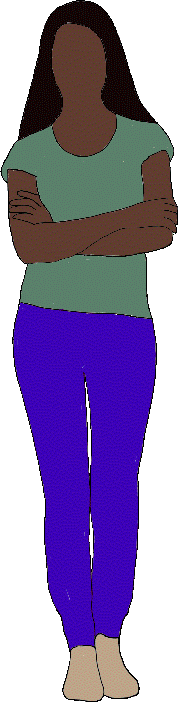
\includegraphics[width=0.04\textwidth]{figures/Relativity/woman_standing}};
}
{
\node[above=-0.5cm] at (-0.01*\L,0) {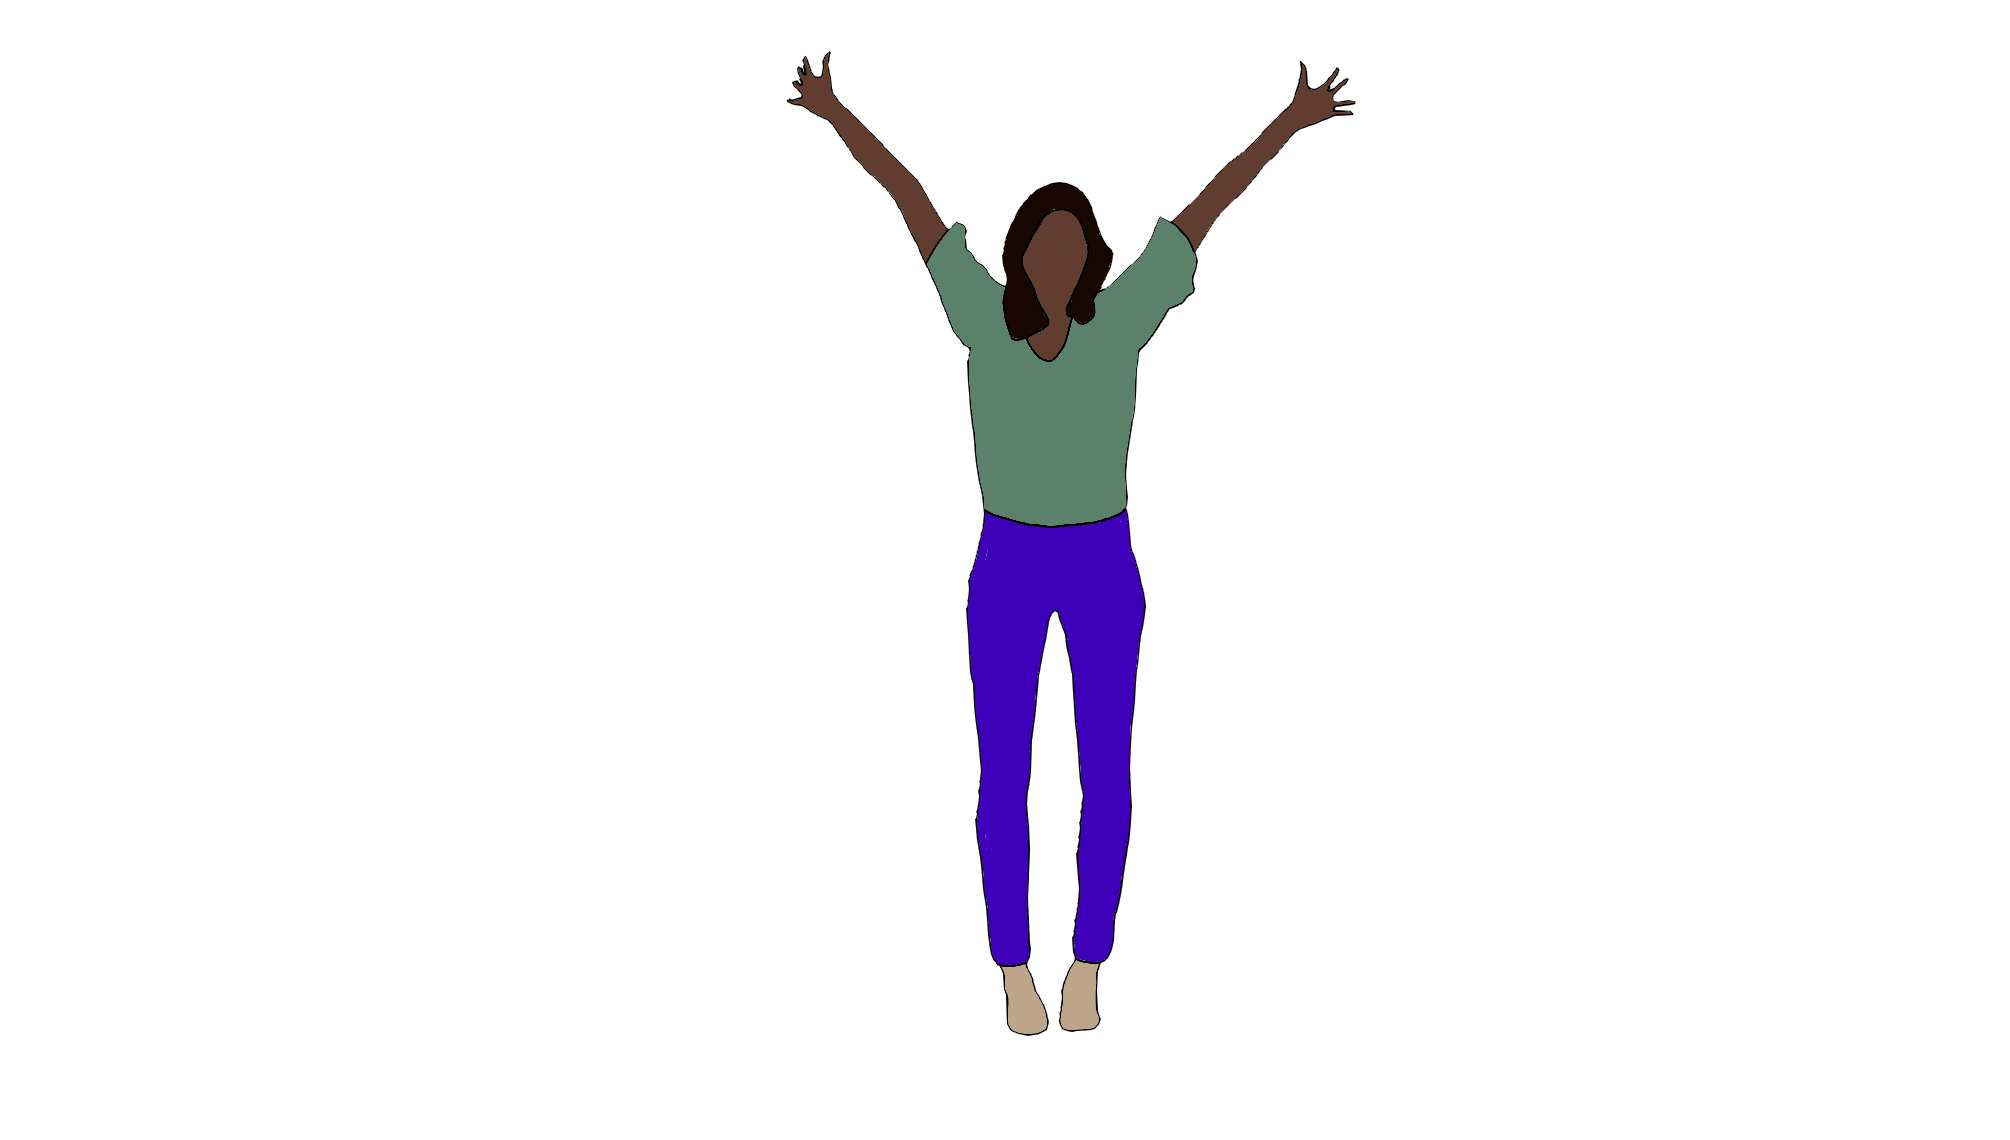
\includegraphics[width=0.4\textwidth]{figures/Relativity/alice_arms_png}};
}


\ifthenelse{\i<6}{
\node[above=-0.2cm] at (-0.4*\L,\h) {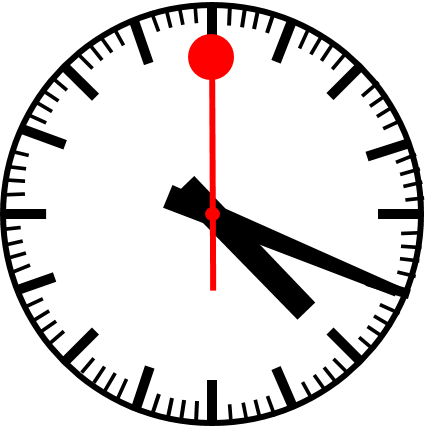
\includegraphics[width=0.07\textwidth]{figures/Relativity/fourtwenty.png}};
}{}
\ifthenelse{\i>5 \AND \i<12}{
\node[above=-0.2cm] at (-0.4*\L,\h) {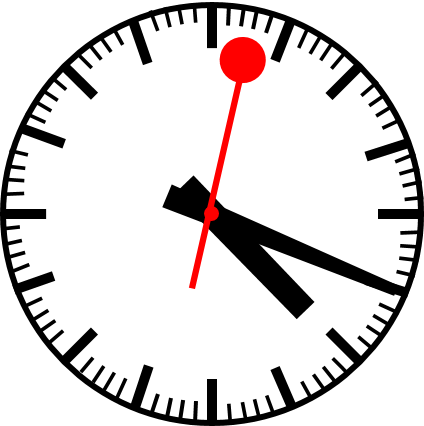
\includegraphics[width=0.07\textwidth]{figures/Relativity/fourtwenty_1.png}};
}{}
\ifthenelse{\i>11 \AND \i<18}{
\node[above=-0.2cm] at (-0.4*\L,\h) {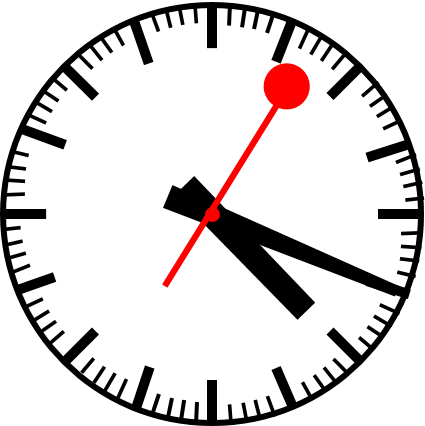
\includegraphics[width=0.07\textwidth]{figures/Relativity/fourtwenty_2.png}};
}{}
\ifthenelse{\i>17}{
\node[above=-0.2cm] at (-0.4*\L,\h) {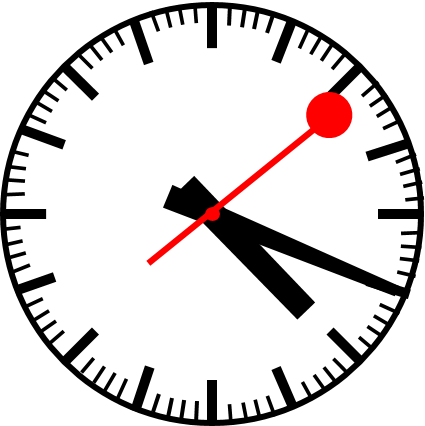
\includegraphics[width=0.07\textwidth]{figures/Relativity/fourtwenty_3.png}};
}{}

\ifthenelse{\i<6}{
\node[above=-0.2cm] at (0.4*\L,\h) {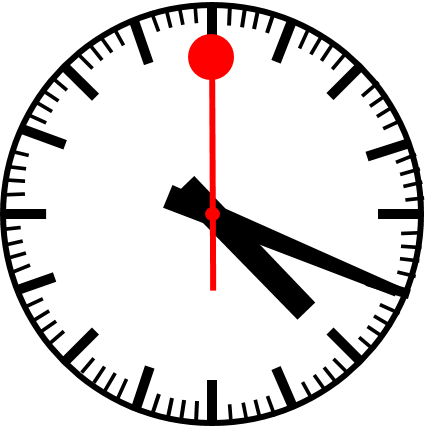
\includegraphics[width=0.07\textwidth]{figures/Relativity/fourtwenty.png}};
}{}
\ifthenelse{\i>5 \AND \i<12}{
\node[above=-0.2cm] at (0.4*\L,\h) {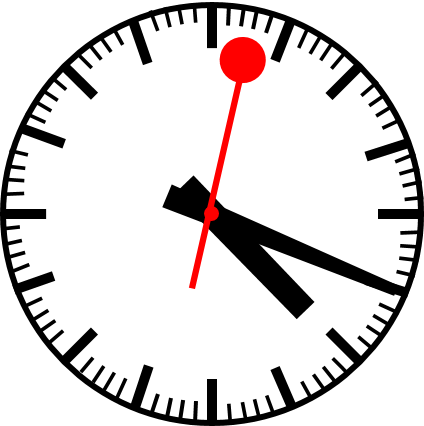
\includegraphics[width=0.07\textwidth]{figures/Relativity/fourtwenty_1.png}};
}{}
\ifthenelse{\i>11 \AND \i<18}{
\node[above=-0.2cm] at (0.4*\L,\h) {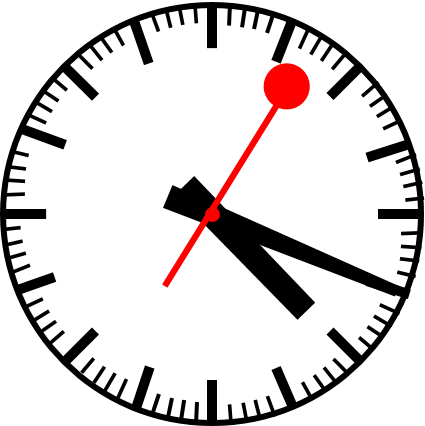
\includegraphics[width=0.07\textwidth]{figures/Relativity/fourtwenty_2.png}};
}{}
\ifthenelse{\i>17}{
\node[above=-0.2cm] at (0.4*\L,\h) {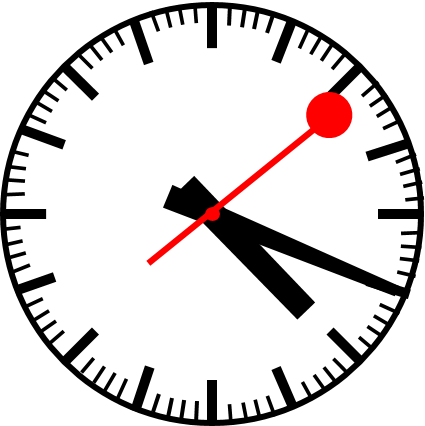
\includegraphics[width=0.07\textwidth]{figures/Relativity/fourtwenty_3.png}};
}{}

\end{tikzpicture}
}%multiframe
\end{animateinline}


\begin{itemize}
\item An observer on a platform is equidistant from 2 clocks that output pulses of light. When the clocks read 16:20, they output a light pulse, the observer sees the two light pulses at the same time and she concludes that the clock are synchronized.
\end{itemize}

\end{frame}


%%%%%%%%%%%%%%%%%%%%%%%%%%%%%%
%% Simultaneity Animation 2
%%%%%%%%%%%%%%%%%%%%%%%%%%%%%%
%%%%%%%%%%%%%%%%%%%%%%%%%%%%%%
\begin{frame}{Recall: Simultaneity}

\centering

\pgfmathtruncatemacro\N{24}
\begin{animateinline}[autoplay,loop]{4} % 5 fps, same as 0.2 s transduration

\multiframe{\N}{i=0+1}{

\tikzmath{
%\i=1;
\L=10;
\w=0.2;%thickness of platform
\h=2;
\D=0.3*\L;
\xs=0.25*\L-\i*0.5*\L/\N;%platform shift
\xr=\xs+0.33*\L-\i*\D/\N;%position of right laser
\xl=-\xs+0.33*\L+\i*\D/\N-1.12*\L;%position of left laser
}
\begin{tikzpicture}

\useasboundingbox (-0.7*\L,-\h) rectangle (0.7*\L,1.5*\h);


%moving platform
\begin{scope}[shift={(\xs,0)}]
%platform
\fill[color=black!70] (-\L/2,-\w) rectangle (\L/2,0);
%posts
\fill[color=qblue!70] (-0.42*\L,0) rectangle (-0.38*\L,0.97*\h);
\fill[color=qblue!70] (0.38*\L,0) rectangle (0.42*\L,0.97*\h);
\ifthenelse{\i<23}{
\node[above=-0.2cm] at (0,0) {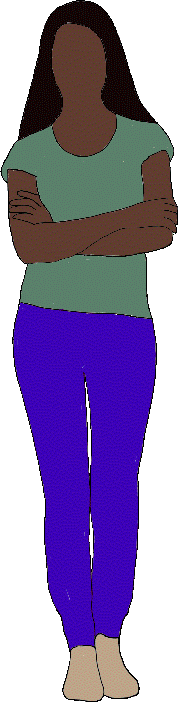
\includegraphics[width=0.04\textwidth]{figures/Relativity/woman_standing}};
}
{
\node[above=-0.5cm] at (-0.01*\L,0) {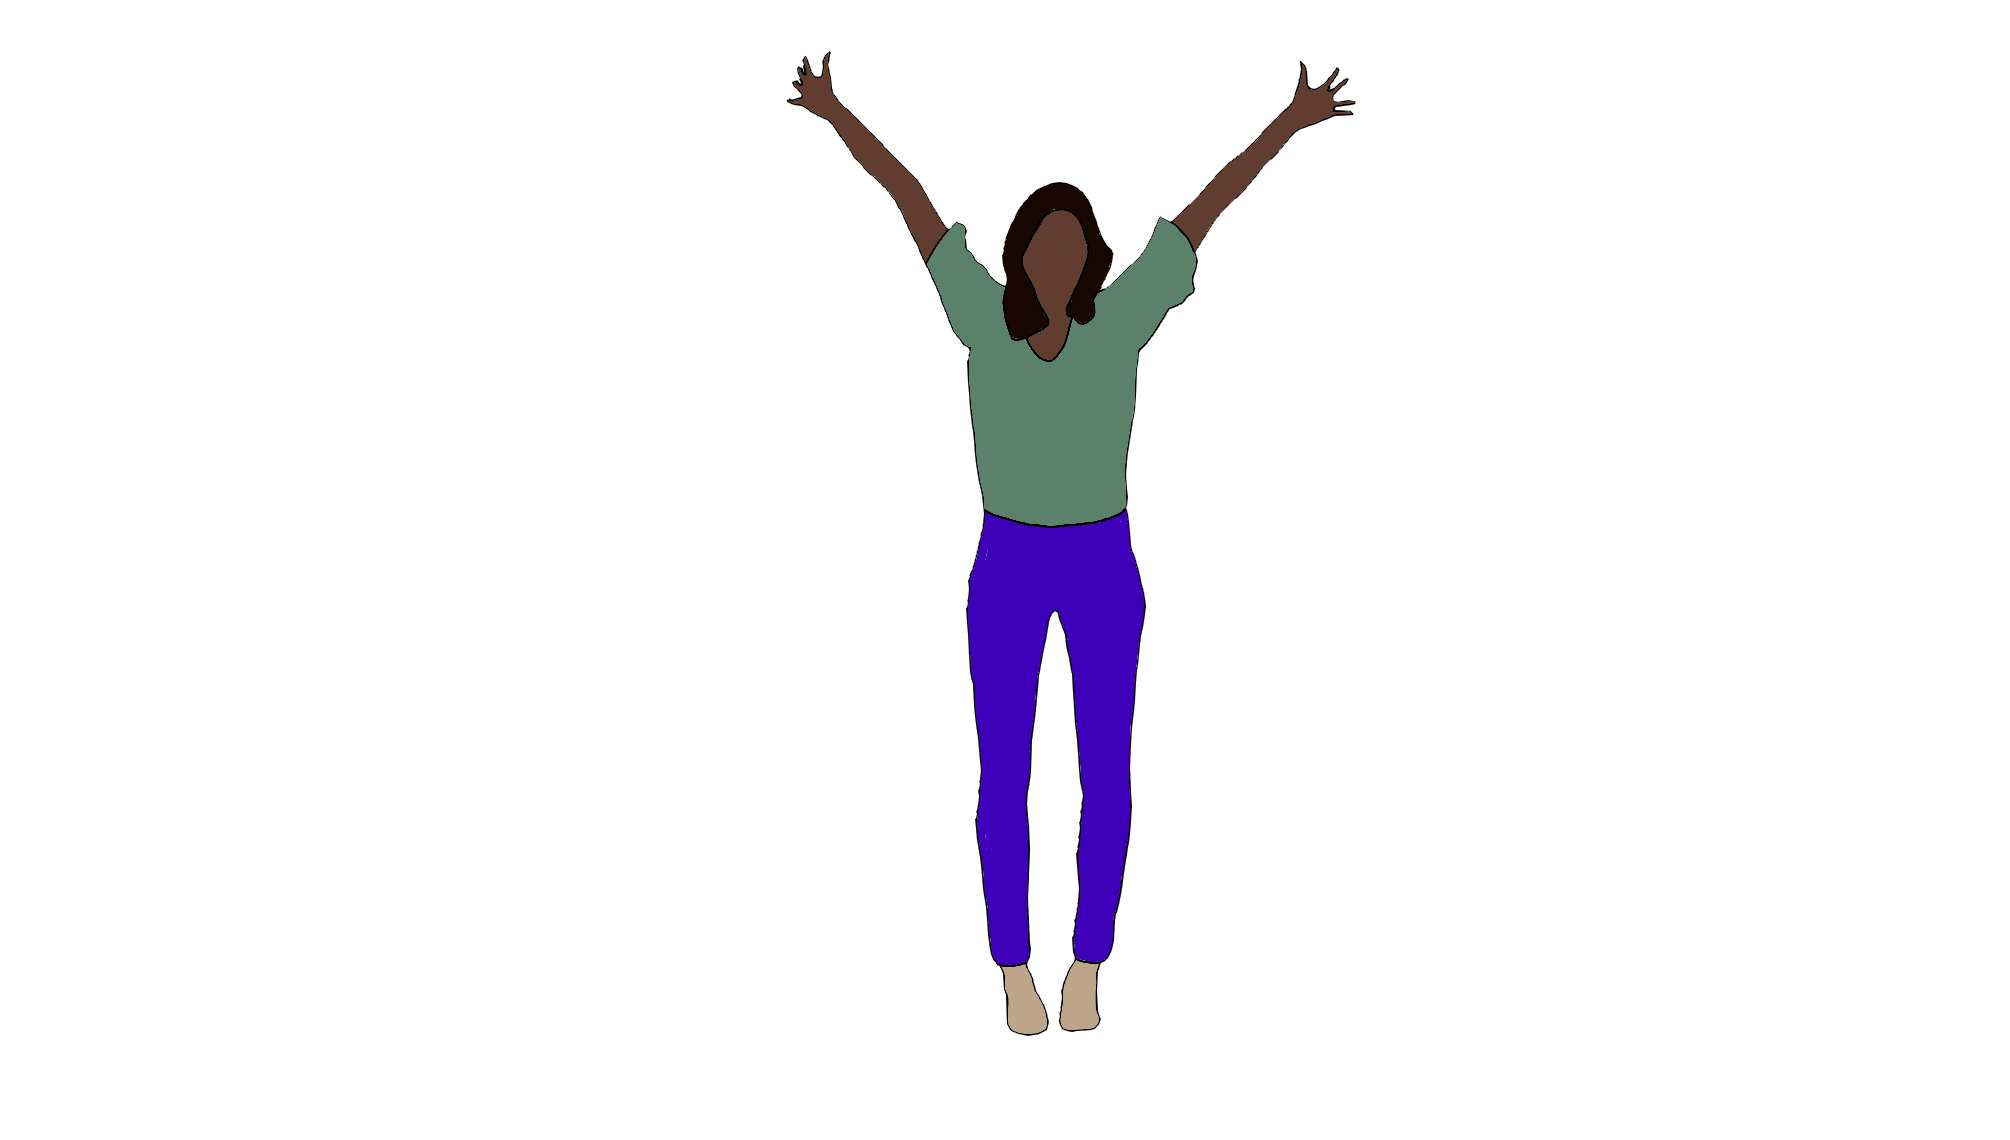
\includegraphics[width=0.4\textwidth]{figures/Relativity/alice_arms_png}};
}

%left clock
\ifthenelse{\i<5}{
\node[above=-0.2cm] at (-0.4*\L,\h) {
\includegraphics[width=0.07\textwidth]{figures/Relativity/fourtwenty_m3.png}};
}{}
\ifthenelse{\i>4 \AND \i<11}{
\node[above=-0.2cm] at (-0.4*\L,\h) {
\includegraphics[width=0.07\textwidth]{figures/Relativity/fourtwenty_m2.png}};
}{}
\ifthenelse{\i>10 \AND \i<17}{
\node[above=-0.2cm] at (-0.4*\L,\h) {
\includegraphics[width=0.07\textwidth]{figures/Relativity/fourtwenty_m1.png}};
}{}
\ifthenelse{\i>16}{
\node[above=-0.2cm] at (-0.4*\L,\h) {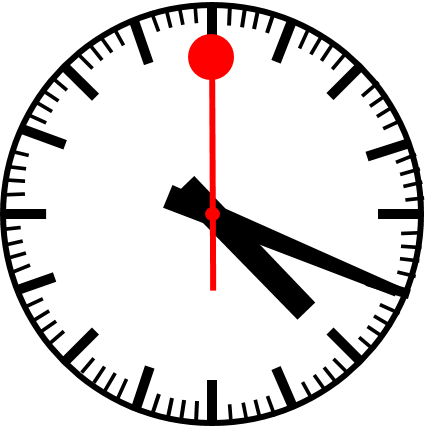
\includegraphics[width=0.07\textwidth]{figures/Relativity/fourtwenty.png}};
}{}


%right clock
\ifthenelse{\i<5}{
\node[above=-0.2cm] at (0.4*\L,\h) {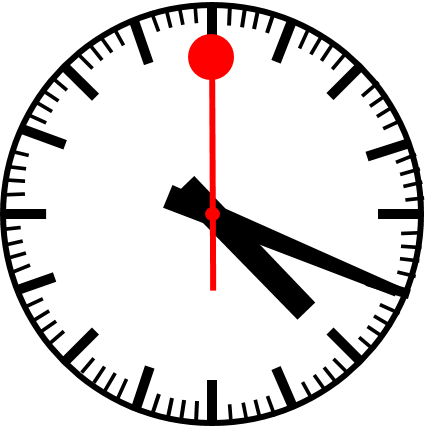
\includegraphics[width=0.07\textwidth]{figures/Relativity/fourtwenty.png}};
}{}
\ifthenelse{\i>4 \AND \i<11}{
\node[above=-0.2cm] at (0.4*\L,\h) {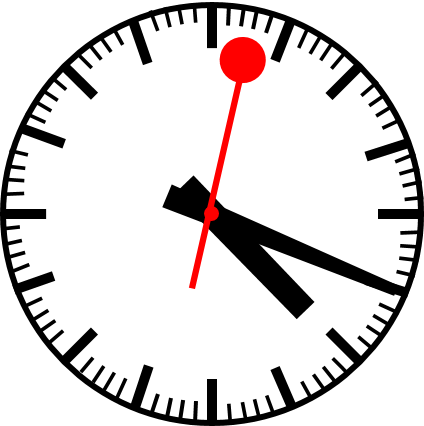
\includegraphics[width=0.07\textwidth]{figures/Relativity/fourtwenty_1.png}};
}{}
\ifthenelse{\i>10 \AND \i<17}{
\node[above=-0.2cm] at (0.4*\L,\h) {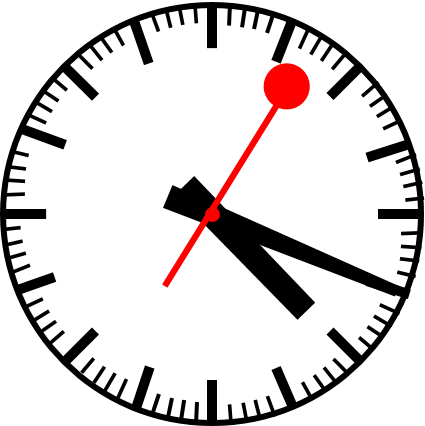
\includegraphics[width=0.07\textwidth]{figures/Relativity/fourtwenty_2.png}};
}{}
\ifthenelse{\i>16}{
\node[above=-0.2cm] at (0.4*\L,\h) {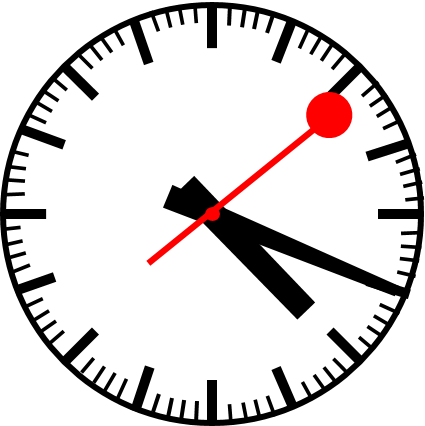
\includegraphics[width=0.07\textwidth]{figures/Relativity/fourtwenty_3.png}};
}{}

\end{scope}

%foreground person
\node[above=-0.5cm] at (-0.5*\L,-0.5*\h) {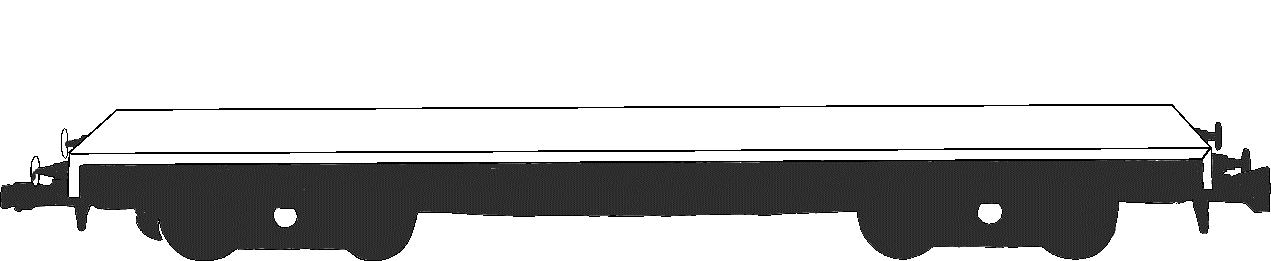
\includegraphics[width=0.4\textwidth]{figures/Relativity/traincart}};
\node[above=0cm] at (-0.5*\L,-0.5*\h) {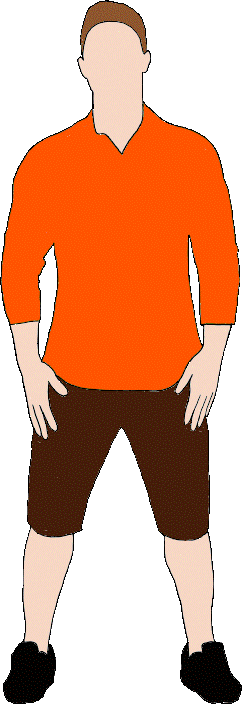
\includegraphics[width=0.06\textwidth]{figures/Relativity/man_standing_ink}};


%laser ball
\draw [color=qred, line width =1.5pt] (\xr,1.2*\h) -- (0.6*\L,1.2*\h);
\node [color=qred, star, star points=10, star point height=.1cm, minimum size=0.2cm, fill] at(\xr,1.2*\h) {};
\ifthenelse{\i>16}{
\draw [color=qred, line width =1.5pt] (\xl,1.2*\h) -- (-0.5*\L,1.2*\h);
\node [color=qred, star, star points=10, star point height=.1cm, minimum size=0.2cm, fill] at(\xl,1.2*\h) {};
}{}

\end{tikzpicture}
}%multiframe
\end{animateinline}

\begin{itemize}
\item An observer on a train sees the platform moving in his rest frame. He observes two pulses of light arrive at the same time at the person on the platform. 
\item He concludes that the pulse from the right happened first, since the pulses travel at speed $c$ and the one from the right traveled further. He disagrees that the clocks are synchronized!
\end{itemize}

\end{frame}




%%%%%%%%%%%%%%%%%%%%%%%%%%%%%%
\subsection{Space-time diagram for platform clocks}
\label{subsec:spcaetimediagramforplatformclocks}
\begin{frame}{Space-time diagram for platform clocks}
Draw the space time diagram for the case of the person on the platform in the middle of the two clocks:
\begin{itemize}
\item Event A: Clock A emits a pulse of light
\item Event B: Clock B emits a pulse of light
\item Event C: The pulses of light meet at the position of the person
\end{itemize}
After drawing this in frame $S$ (the platform), draw $S’$ on top of that (the frame for the moving train), and compare the locations of $A$ and $B$…
\capfig{0.5}{figures/Relativity/platform}{In the reference frame at rest relative to the clocks, they appear synchronized, emitting pulses of light at the same time.}
\end{frame}



%%%%%%%%%%%%%%%%%%%%%%%%%%%%%%
\twocolframe{Space-time diagram for platform clocks}
{
\only<1>{
\capfig{0.9}{figures/Relativity/platform_rest}{In the reference frame at rest relative to the clocks.}
}
\only<2>{
\capfig{0.9}{figures/Relativity/platform_moving}{In the reference frame moving relative to the clocks.}
}
\only<3>{
\scalebox{-1}[1]{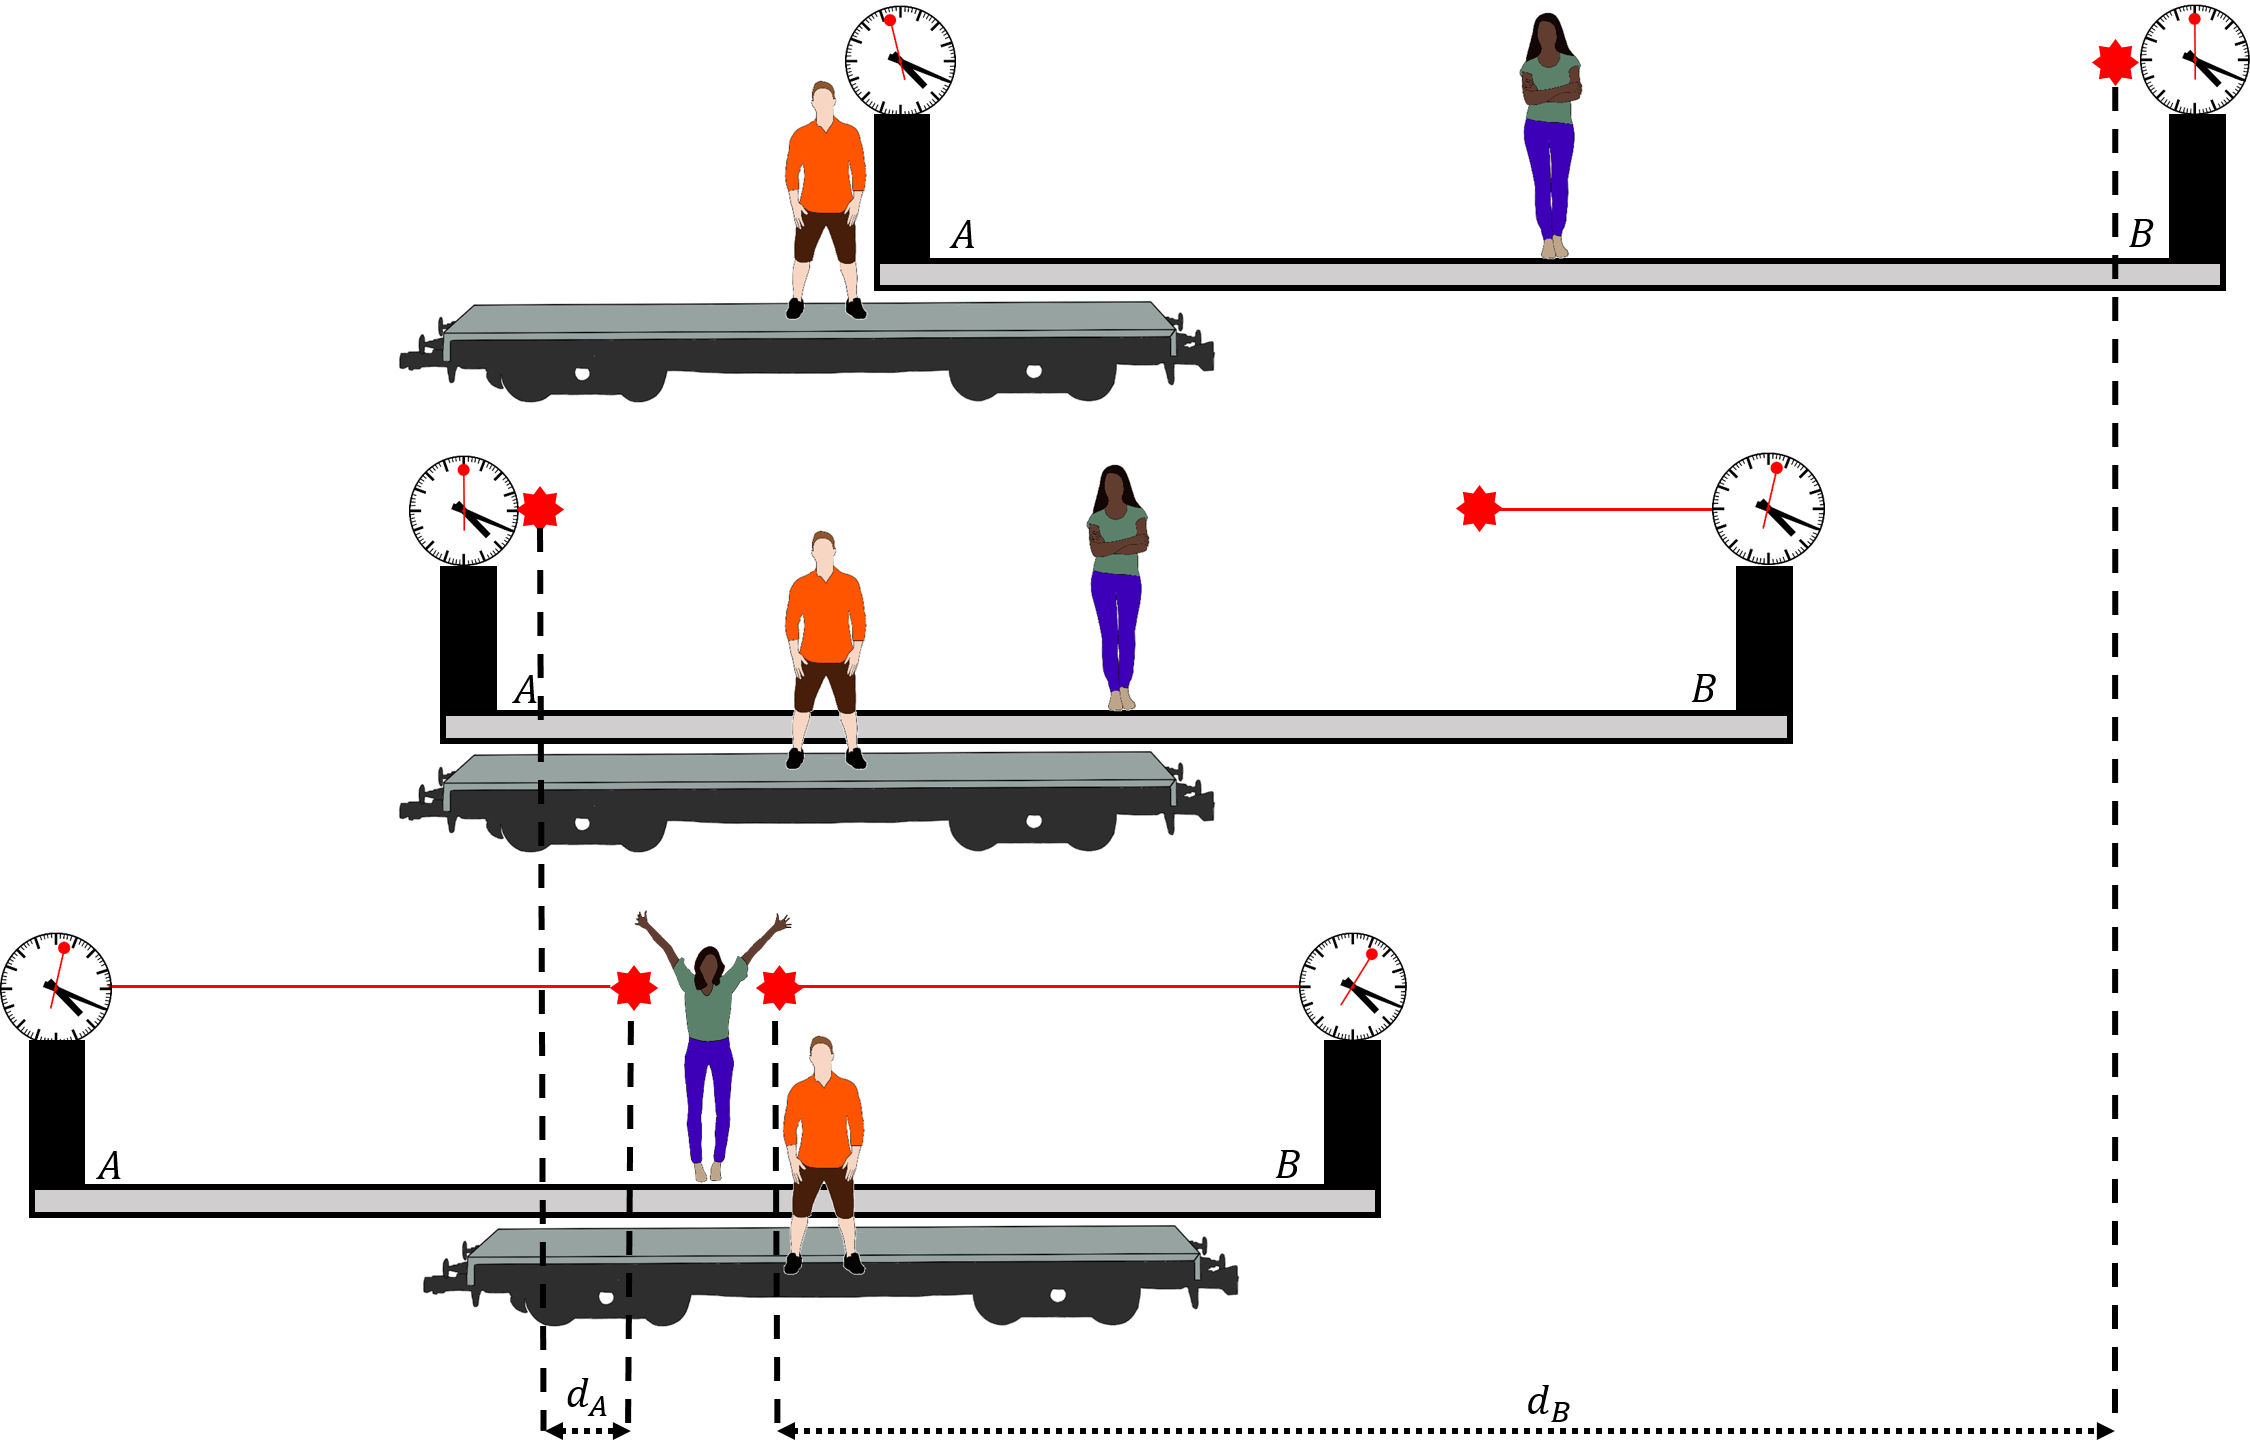
\includegraphics[width=0.9\textwidth]{figures/Relativity/platform_moving}}
\captionof*{figure}{\textit{In the reference frame moving relative to the clocks, going the other way.}}
}
}
{
\centering
\begin{tikzpicture}
\tikzmath{
\L=4.5;
\EAx=-0.3*\L;
\EAy=0.*\L;
\EBx=0.3*\L;
\EBy=0.*\L;
\ECx=0;
\ECy=\EBx;
\th=20;
\v=1.*tan(\th);
}
\coordinate (EA) at (\EAx,\EAy);
\coordinate (EB) at (\EBx,\EBy);
\coordinate (EC) at (\ECx,\ECy);
\coordinate (OO) at (0,0);

\draw[-latex,line width = 1] (-0.5*\L,0) -- (0.75*\L,0) node[below] {$x$};
\draw[-latex,line width = 1] (0,-0.5*\L) -- (0,0.75*\L) node[left] {$ct$};

\fill (EA) circle(2pt) node[above]{$A$};
\fill (EB) circle(2pt) node[above]{$B$};
\fill (EC) circle(2pt) node[left]{$C$};

\draw[color=qred,line width = 1] (EA) -- (EC);
\draw[color=qred,line width = 1] (EB) -- (EC);

%S' axes
\only<3>{
\tikzmath{\th=-20;}
}

\only<2->{
\draw[-latex,color=qblue!70,line width = 1] (\th:-0.5*\L) -- (\th:0.75*\L) node[below] {$x'$};
\draw[-latex,color=qblue!70,line width = 1] ({90-\th}:-0.5*\L) -- ({90-\th}:0.75*\L) node[left] {$ct'$};

\coordinate (XP) at ($(0,0)+(\th:0.3*\L)$);
\coordinate (YP) at ($(0,0)+({90-\th}:0.3*\L)$);
\coordinate (EAYP) at ($(EA)+(\th:0.3*\L)$);
\coordinate (EAy) at (intersection of EA--EAYP and OO--YP);
\coordinate (EBYP) at ($(EB)+(\th:0.3*\L)$);
\coordinate (EBy) at (intersection of EB--EBYP and OO--YP);
\coordinate (ECYP) at ($(EC)+(\th:0.3*\L)$);
\coordinate (ECy) at (intersection of EC--ECYP and OO--YP);

\draw[dashed,color=qblue!70] (EA) -- (EAy);
\fill[color=qblue!70] (EAy) circle(2pt);
\draw[dashed,color=qblue!70] (EB) -- (EBy);
\fill[color=qblue!70] (EBy) circle(2pt);
\draw[dashed,color=qblue!70] (EC) -- (ECy);
\fill[color=qblue!70] (ECy) circle(2pt);
}
\end{tikzpicture}
\captionof*{figure}{\textit{Space-time diagram for platform clocks}}
}


%%%%%%%%%%%%%%%%%%%%%%%%%%%%%%
\begin{frame}{The Train Paradox}
\capfig{1}{figures/Relativity/barn}{}
\vspace{-1cm}
\begin{itemize}
\item As seen from the ground, the train that is contracted to a length of \SI{200}{m} fits in the tunnel of the same length. As seen in the train, the \SI{500}{m} train does not fit in the \SI{80}{m} tunnel. 
\item A person on Earth briefly closes the doors of the tunnel while the train is inside, nothing happens to the train, since it fits. To the observer on the train, was the train just destroyed?
\end{itemize}
\end{frame}

%%%%%%%%%%%%%%%%%%%%%%%%%%%%%%


%%%%%%%%%%%%%%%






%%%%%%%%%%%%%%%%%%%%%%%





%%%%%%%%%%%%%%%%%%%%%%





%%%%%%%%%%%%%%%%%%%%%%%





%%%%%%%%%%%%%%%%%%%%%%



%%%%%%%%%%%%%%%%%%%%%%%%%%%%




%%%%%%%%%%%%%%%%%%%%%%%%%




%%%%%%%%%%%%%%%%%%%%%%%%%





%%%%%%%%%%%%%%%%%%%%%%%%%%




%%%%%%%%%%%%%%%%%%%%%%%%%%%%%%%%%%%






%%%%%%%%%%%%%%%%%%%%%%%%%%%%%%%%%%%%%





%%%%%%%%%%%%%%%%%%%%%%%%%%%%%%%%%%%%%%%%




%%%%%%%%%%%%%%%%%%%%%%%%%%%%%%%%%%%%%%%%%%%%



%%%%%%%%%%%%%%%%%%%%%%%%%%%%%%



%%%%%%%%%%%%%%%%%%%%%%%%%%%%%%%



%%%%%%%%%%%%%%%%%%%%%%%%%%%%%%%%%%%



%%%%%%%%%%%%%%%%%%%%%%%%%%%%%%%%%%



%%%%%%%%%%%%%%%%%%%%%%%%%%%%%%%%




%%%%%%%%%%%%%%%%%%%%%%%%%%%%



%%%%%%%%%%%%%%%%%%%%%%%%%%%%%




%%%%%%%%%%%%%%%%%%%%%%%%%%%%%%%%



%%%%%%%%%%%%%%%%%%%%%%%%%%%%%%%%


%%%%%%%%%%%%%%%%%%%%%%%%%%%%%%%%



%%%%%%%%%%%%%%%%%%%%%%%%%%%%%%%%



%%%%%%%%%%%%%%%%%%%%%%%%%%%%%%%%



%%%%%%%%%%%%%%%%%%%%%%%%%%%%%%%%



%%%%%%%%%%%%%%%%%%%%%%%%%%%%%%%%



%%%%%%%%%%%%%%%%%%%%%%%%%%%%%%%%



%%%%%%%%%%%%%%%%%%%%%%%%%%%%%%%%



%%%%%%%%%%%%%%%%%%%%%%%%%%%%%%%%



%%%%%%%%%%%%%%%%%%%%%%%%%%%%%%%%







































\end{document}